\documentclass[twoside]{book}

% Packages required by doxygen
\usepackage{fixltx2e}
\usepackage{calc}
\usepackage{doxygen}
\usepackage{graphicx}
\usepackage[utf8]{inputenc}
\usepackage{makeidx}
\usepackage{multicol}
\usepackage{multirow}
\PassOptionsToPackage{warn}{textcomp}
\usepackage{textcomp}
\usepackage[nointegrals]{wasysym}
\usepackage[table]{xcolor}

% Font selection
\usepackage[T1]{fontenc}
\usepackage{mathptmx}
\usepackage[scaled=.90]{helvet}
\usepackage{courier}
\usepackage{amssymb}
\usepackage{sectsty}
\renewcommand{\familydefault}{\sfdefault}
\allsectionsfont{%
  \fontseries{bc}\selectfont%
  \color{darkgray}%
}
\renewcommand{\DoxyLabelFont}{%
  \fontseries{bc}\selectfont%
  \color{darkgray}%
}
\newcommand{\+}{\discretionary{\mbox{\scriptsize$\hookleftarrow$}}{}{}}

% Page & text layout
\usepackage{geometry}
\geometry{%
  a4paper,%
  top=2.5cm,%
  bottom=2.5cm,%
  left=2.5cm,%
  right=2.5cm%
}
\tolerance=750
\hfuzz=15pt
\hbadness=750
\setlength{\emergencystretch}{15pt}
\setlength{\parindent}{0cm}
\setlength{\parskip}{0.2cm}
\makeatletter
\renewcommand{\paragraph}{%
  \@startsection{paragraph}{4}{0ex}{-1.0ex}{1.0ex}{%
    \normalfont\normalsize\bfseries\SS@parafont%
  }%
}
\renewcommand{\subparagraph}{%
  \@startsection{subparagraph}{5}{0ex}{-1.0ex}{1.0ex}{%
    \normalfont\normalsize\bfseries\SS@subparafont%
  }%
}
\makeatother

% Headers & footers
\usepackage{fancyhdr}
\pagestyle{fancyplain}
\fancyhead[LE]{\fancyplain{}{\bfseries\thepage}}
\fancyhead[CE]{\fancyplain{}{}}
\fancyhead[RE]{\fancyplain{}{\bfseries\leftmark}}
\fancyhead[LO]{\fancyplain{}{\bfseries\rightmark}}
\fancyhead[CO]{\fancyplain{}{}}
\fancyhead[RO]{\fancyplain{}{\bfseries\thepage}}
\fancyfoot[LE]{\fancyplain{}{}}
\fancyfoot[CE]{\fancyplain{}{}}
\fancyfoot[RE]{\fancyplain{}{\bfseries\scriptsize Generated on Tue Oct 21 2014 10\+:18\+:16 for Yavin I\+V Death Star Tracker by Doxygen }}
\fancyfoot[LO]{\fancyplain{}{\bfseries\scriptsize Generated on Tue Oct 21 2014 10\+:18\+:16 for Yavin I\+V Death Star Tracker by Doxygen }}
\fancyfoot[CO]{\fancyplain{}{}}
\fancyfoot[RO]{\fancyplain{}{}}
\renewcommand{\footrulewidth}{0.4pt}
\renewcommand{\chaptermark}[1]{%
  \markboth{#1}{}%
}
\renewcommand{\sectionmark}[1]{%
  \markright{\thesection\ #1}%
}

% Indices & bibliography
\usepackage{natbib}
\usepackage[titles]{tocloft}
\setcounter{tocdepth}{3}
\setcounter{secnumdepth}{5}
\makeindex

% Hyperlinks (required, but should be loaded last)
\usepackage{ifpdf}
\ifpdf
  \usepackage[pdftex,pagebackref=true]{hyperref}
\else
  \usepackage[ps2pdf,pagebackref=true]{hyperref}
\fi
\hypersetup{%
  colorlinks=true,%
  linkcolor=blue,%
  citecolor=blue,%
  unicode%
}

% Custom commands
\newcommand{\clearemptydoublepage}{%
  \newpage{\pagestyle{empty}\cleardoublepage}%
}


%===== C O N T E N T S =====

\begin{document}

% Titlepage & ToC
\hypersetup{pageanchor=false,
             bookmarks=true,
             bookmarksnumbered=true,
             pdfencoding=unicode
            }
\pagenumbering{roman}
\begin{titlepage}
\vspace*{7cm}
\begin{center}%
{\Large Yavin I\+V Death Star Tracker \\[1ex]\large V1.\+0 }\\
\vspace*{1cm}
{\large Generated by Doxygen 1.8.8}\\
\vspace*{0.5cm}
{\small Tue Oct 21 2014 10:18:16}\\
\end{center}
\end{titlepage}
\clearemptydoublepage
\tableofcontents
\clearemptydoublepage
\pagenumbering{arabic}
\hypersetup{pageanchor=true}

%--- Begin generated contents ---
\chapter{Todo List}
\label{todo}
\hypertarget{todo}{}

\begin{DoxyRefList}
\item[\label{todo__todo000001}%
\hypertarget{todo__todo000001}{}%
File \hyperlink{ConfigRegs18f4520_8h}{Config\+Regs18f4520.h} ]Consider if Watchdog Timer should be enabled for production code, and add W\+D\+T management code if so.

Consider if Stack Overflow Reset should be enabled for production code. It may be better not to, as there is no re-\/entrant or recursive code, or dynamic memory allocation here -\/ if the code loads statically it should run.

Change startup code c016iz.\+c so that everything (including initialised variables) correctly re-\/starts if \hyperlink{HardUItest_8c_a6288eba0f8e8ad3ab1544ad731eb7667}{main()} ever exits or a B\+O\+R or W\+D\+T reset occurs.  
\item[\label{todo__todo000004}%
\hypertarget{todo__todo000004}{}%
Global \hyperlink{LCD_8c_a6d7066138d22070be0234d8b113cf776}{delay} (unsigned int t)]Complete, test, debug and document this code!!! 
\item[\label{todo__todo000005}%
\hypertarget{todo__todo000005}{}%
Global \hyperlink{Range_8h_aff3698f3a7b3b5963d8e6b305a165d71}{range} (void)]Read in temperature for U\+S calculation  
\item[\label{todo__todo000006}%
\hypertarget{todo__todo000006}{}%
Global \hyperlink{Temp_8h_a4946ccbc1990e831667bffded1147c4f}{read\+Tempx2} (void)]Test and debug this function 
\end{DoxyRefList}
\chapter{Data Structure Index}
\section{Data Structures}
Here are the data structures with brief descriptions\+:\begin{DoxyCompactList}
\item\contentsline{section}{\hyperlink{structcircularBuffer}{circular\+Buffer} \\*Stores bytes of data in a circular buffer }{\pageref{structcircularBuffer}}{}
\item\contentsline{section}{\hyperlink{structDelay}{Delay} }{\pageref{structDelay}}{}
\item\contentsline{section}{\hyperlink{structDirection}{Direction} \\*Stores an inclination and azimuth }{\pageref{structDirection}}{}
\item\contentsline{section}{\hyperlink{structSubMenu}{Sub\+Menu} }{\pageref{structSubMenu}}{}
\item\contentsline{section}{\hyperlink{structsystemState}{system\+State} \\*Stores the current state of the system }{\pageref{structsystemState}}{}
\item\contentsline{section}{\hyperlink{structTrackingData}{Tracking\+Data} \\*Stores the current target information }{\pageref{structTrackingData}}{}
\end{DoxyCompactList}

\chapter{File Index}
\section{File List}
Here is a list of all files with brief descriptions\+:\begin{DoxyCompactList}
\item\contentsline{section}{Yavin4\+Defence\+System/\+Code/\hyperlink{CircularBuffers_8h}{Circular\+Buffers.\+h} }{\pageref{CircularBuffers_8h}}{}
\item\contentsline{section}{Yavin4\+Defence\+System/\+Code/\hyperlink{Common_8h}{Common.\+h} }{\pageref{Common_8h}}{}
\item\contentsline{section}{Yavin4\+Defence\+System/\+Code/\hyperlink{ConfigRegs18f4520_8h}{Config\+Regs18f4520.\+h} \\*Include file to set the Configuration Bits of a P\+I\+C18\+F4520 }{\pageref{ConfigRegs18f4520_8h}}{}
\item\contentsline{section}{Yavin4\+Defence\+System/\+Code/\hyperlink{EEPROM_8c}{E\+E\+P\+R\+O\+M.\+c} }{\pageref{EEPROM_8c}}{}
\item\contentsline{section}{Yavin4\+Defence\+System/\+Code/\hyperlink{HardUItest_8c}{Hard\+U\+Itest.\+c} }{\pageref{HardUItest_8c}}{}
\item\contentsline{section}{Yavin4\+Defence\+System/\+Code/\hyperlink{HardUItest_8h}{Hard\+U\+Itest.\+h} }{\pageref{HardUItest_8h}}{}
\item\contentsline{section}{Yavin4\+Defence\+System/\+Code/\hyperlink{Interrupts_8c}{Interrupts.\+c} }{\pageref{Interrupts_8c}}{}
\item\contentsline{section}{Yavin4\+Defence\+System/\+Code/\hyperlink{LCD_8c}{L\+C\+D.\+c} }{\pageref{LCD_8c}}{}
\item\contentsline{section}{Yavin4\+Defence\+System/\+Code/\hyperlink{LCD_8h}{L\+C\+D.\+h} }{\pageref{LCD_8h}}{}
\item\contentsline{section}{Yavin4\+Defence\+System/\+Code/\hyperlink{LCD__defs_8h}{L\+C\+D\+\_\+defs.\+h} }{\pageref{LCD__defs_8h}}{}
\item\contentsline{section}{Yavin4\+Defence\+System/\+Code/\hyperlink{MenuDefs_8h}{Menu\+Defs.\+h} }{\pageref{MenuDefs_8h}}{}
\item\contentsline{section}{Yavin4\+Defence\+System/\+Code/\hyperlink{Menusystem_8c}{Menusystem.\+c} }{\pageref{Menusystem_8c}}{}
\item\contentsline{section}{Yavin4\+Defence\+System/\+Code/\hyperlink{Menusystem_8h}{Menusystem.\+h} }{\pageref{Menusystem_8h}}{}
\item\contentsline{section}{Yavin4\+Defence\+System/\+Code/\hyperlink{Menusystem2_8c}{Menusystem2.\+c} }{\pageref{Menusystem2_8c}}{}
\item\contentsline{section}{Yavin4\+Defence\+System/\+Code/\hyperlink{newfile_8h}{newfile.\+h} }{\pageref{newfile_8h}}{}
\item\contentsline{section}{Yavin4\+Defence\+System/\+Code/\hyperlink{newmain_8c}{newmain.\+c} }{\pageref{newmain_8c}}{}
\item\contentsline{section}{Yavin4\+Defence\+System/\+Code/\hyperlink{p18f4520_8h}{p18f4520.\+h} }{\pageref{p18f4520_8h}}{}
\item\contentsline{section}{Yavin4\+Defence\+System/\+Code/\hyperlink{PanTilt_8c}{Pan\+Tilt.\+c} }{\pageref{PanTilt_8c}}{}
\item\contentsline{section}{Yavin4\+Defence\+System/\+Code/\hyperlink{PanTilt_8h}{Pan\+Tilt.\+h} }{\pageref{PanTilt_8h}}{}
\item\contentsline{section}{Yavin4\+Defence\+System/\+Code/\hyperlink{Range_8c}{Range.\+c} }{\pageref{Range_8c}}{}
\item\contentsline{section}{Yavin4\+Defence\+System/\+Code/\hyperlink{Range_8h}{Range.\+h} }{\pageref{Range_8h}}{}
\item\contentsline{section}{Yavin4\+Defence\+System/\+Code/\hyperlink{ROM2RAM_8c}{R\+O\+M2\+R\+A\+M.\+c} }{\pageref{ROM2RAM_8c}}{}
\item\contentsline{section}{Yavin4\+Defence\+System/\+Code/\hyperlink{Serial_8c}{Serial.\+c} }{\pageref{Serial_8c}}{}
\item\contentsline{section}{Yavin4\+Defence\+System/\+Code/\hyperlink{Serial_8h}{Serial.\+h} }{\pageref{Serial_8h}}{}
\item\contentsline{section}{Yavin4\+Defence\+System/\+Code/\hyperlink{Temp_8c}{Temp.\+c} }{\pageref{Temp_8c}}{}
\item\contentsline{section}{Yavin4\+Defence\+System/\+Code/\hyperlink{Temp_8h}{Temp.\+h} }{\pageref{Temp_8h}}{}
\item\contentsline{section}{Yavin4\+Defence\+System/\+Code/\hyperlink{Tracking_8c}{Tracking.\+c} }{\pageref{Tracking_8c}}{}
\item\contentsline{section}{Yavin4\+Defence\+System/\+Code/\hyperlink{Tracking_8h}{Tracking.\+h} }{\pageref{Tracking_8h}}{}
\item\contentsline{section}{Yavin4\+Defence\+System/\+Code/\hyperlink{usart_8h}{usart.\+h} }{\pageref{usart_8h}}{}
\item\contentsline{section}{Yavin4\+Defence\+System/\+Code/\hyperlink{User__Interface_8c}{User\+\_\+\+Interface.\+c} }{\pageref{User__Interface_8c}}{}
\item\contentsline{section}{Yavin4\+Defence\+System/\+Code/\hyperlink{User__Interface_8h}{User\+\_\+\+Interface.\+h} }{\pageref{User__Interface_8h}}{}
\end{DoxyCompactList}

\chapter{Data Structure Documentation}
\hypertarget{structcircular_buffer}{\section{circular\+Buffer Struct Reference}
\label{structcircular_buffer}\index{circular\+Buffer@{circular\+Buffer}}
}


Stores bytes of data in a circular buffer.  




{\ttfamily \#include $<$Circular\+Buffers.\+h$>$}

\subsection*{Data Fields}
\begin{DoxyCompactItemize}
\item 
unsigned char \hyperlink{structcircular_buffer_a47f7e6109597e5c1c227993c0ce5f560}{head}
\item 
unsigned char \hyperlink{structcircular_buffer_af18a1d7542e277284c4794593b049258}{tail}
\item 
unsigned char \hyperlink{structcircular_buffer_ad7b57ba90694482456be1fbab7de4aec}{data} \mbox{[}\hyperlink{_circular_buffers_8h_a5a69f707d5405fe875b322c6bfbace46}{B\+U\+F\+F\+E\+R\+L\+E\+N\+G\+T\+H}\mbox{]}
\end{DoxyCompactItemize}


\subsection{Detailed Description}
Stores bytes of data in a circular buffer. 



 typedef of \hyperlink{structcircular_buffer}{circular\+Buffer} struct

Length\+: B\+U\+F\+F\+E\+R\+L\+E\+N\+G\+T\+H

Description\+: Defines a circular buffer in which bytes of data can be placed, or removed at any time in the correct order that they were pushed. The accompanying functionality facilitates all necessary circular buffer related operations. This implementation reduces the buffer length by 1 to differentiate between full and empty states. B\+U\+F\+F\+E\+R\+L\+E\+N\+G\+T\+H can be redefined in individual files to get different buffer lengths 

Definition at line 49 of file Circular\+Buffers.\+h.



\subsection{Field Documentation}
\hypertarget{structcircular_buffer_ad7b57ba90694482456be1fbab7de4aec}{\index{circular\+Buffer@{circular\+Buffer}!data@{data}}
\index{data@{data}!circular\+Buffer@{circular\+Buffer}}
\subsubsection[{data}]{\setlength{\rightskip}{0pt plus 5cm}unsigned char data\mbox{[}{\bf B\+U\+F\+F\+E\+R\+L\+E\+N\+G\+T\+H}\mbox{]}}}\label{structcircular_buffer_ad7b57ba90694482456be1fbab7de4aec}


Definition at line 53 of file Circular\+Buffers.\+h.

\hypertarget{structcircular_buffer_a47f7e6109597e5c1c227993c0ce5f560}{\index{circular\+Buffer@{circular\+Buffer}!head@{head}}
\index{head@{head}!circular\+Buffer@{circular\+Buffer}}
\subsubsection[{head}]{\setlength{\rightskip}{0pt plus 5cm}unsigned char head}}\label{structcircular_buffer_a47f7e6109597e5c1c227993c0ce5f560}


Definition at line 51 of file Circular\+Buffers.\+h.

\hypertarget{structcircular_buffer_af18a1d7542e277284c4794593b049258}{\index{circular\+Buffer@{circular\+Buffer}!tail@{tail}}
\index{tail@{tail}!circular\+Buffer@{circular\+Buffer}}
\subsubsection[{tail}]{\setlength{\rightskip}{0pt plus 5cm}unsigned char tail}}\label{structcircular_buffer_af18a1d7542e277284c4794593b049258}


Definition at line 52 of file Circular\+Buffers.\+h.



The documentation for this struct was generated from the following file\+:\begin{DoxyCompactItemize}
\item 
\hyperlink{_circular_buffers_8h}{Circular\+Buffers.\+h}\end{DoxyCompactItemize}

\hypertarget{struct_delay}{\section{Delay Struct Reference}
\label{struct_delay}\index{Delay@{Delay}}
}
\subsection*{Public Attributes}
\begin{DoxyCompactItemize}
\item 
\hypertarget{struct_delay_a4cb4f750cd566d1a1cf61d1fa93d5ce3}{signed int {\bfseries Azimuth\+Delay}}\label{struct_delay_a4cb4f750cd566d1a1cf61d1fa93d5ce3}

\item 
\hypertarget{struct_delay_a19ac2a6a70e80fc14128af5716580d12}{signed int {\bfseries Inclination\+Delay}}\label{struct_delay_a19ac2a6a70e80fc14128af5716580d12}

\end{DoxyCompactItemize}


The documentation for this struct was generated from the following file\+:\begin{DoxyCompactItemize}
\item 
Pan\+Tilt.\+c\end{DoxyCompactItemize}

\hypertarget{struct_direction}{\section{Direction Struct Reference}
\label{struct_direction}\index{Direction@{Direction}}
}


Stores an inclination and azimuth.  




{\ttfamily \#include $<$Common.\+h$>$}

\subsection*{Data Fields}
\begin{DoxyCompactItemize}
\item 
int \hyperlink{struct_direction_a866e78e12cb32dcaf1ded89bda8be8f5}{azimuth}
\item 
int \hyperlink{struct_direction_af308b9934394c8bcf7614eb1df2d863f}{inclination}
\end{DoxyCompactItemize}


\subsection{Detailed Description}
Stores an inclination and azimuth. 



 typedef of \hyperlink{struct_direction}{Direction} struct

Description\+: A fully defined direction in which to point the pan tilt actuator or any other such purpose

Elements\+: -\/\+Azimuth\+: Contains the azimuth component of the direction (generally degrees) -\/\+Inclination\+: Contains the inclination component of the direction (generally degrees) 

Definition at line 70 of file Common.\+h.



\subsection{Field Documentation}
\hypertarget{struct_direction_a866e78e12cb32dcaf1ded89bda8be8f5}{\index{Direction@{Direction}!azimuth@{azimuth}}
\index{azimuth@{azimuth}!Direction@{Direction}}
\subsubsection[{azimuth}]{\setlength{\rightskip}{0pt plus 5cm}int azimuth}}\label{struct_direction_a866e78e12cb32dcaf1ded89bda8be8f5}


Definition at line 72 of file Common.\+h.

\hypertarget{struct_direction_af308b9934394c8bcf7614eb1df2d863f}{\index{Direction@{Direction}!inclination@{inclination}}
\index{inclination@{inclination}!Direction@{Direction}}
\subsubsection[{inclination}]{\setlength{\rightskip}{0pt plus 5cm}int inclination}}\label{struct_direction_af308b9934394c8bcf7614eb1df2d863f}


Definition at line 73 of file Common.\+h.



The documentation for this struct was generated from the following file\+:\begin{DoxyCompactItemize}
\item 
\hyperlink{_common_8h}{Common.\+h}\end{DoxyCompactItemize}

\hypertarget{struct_sub_menu}{\section{Sub\+Menu Struct Reference}
\label{struct_sub_menu}\index{Sub\+Menu@{Sub\+Menu}}
}


Collaboration diagram for Sub\+Menu\+:\nopagebreak
\begin{figure}[H]
\begin{center}
\leavevmode
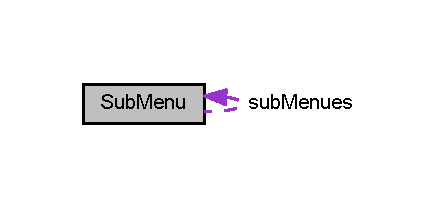
\includegraphics[width=210pt]{struct_sub_menu__coll__graph}
\end{center}
\end{figure}
\subsection*{Data Fields}
\begin{DoxyCompactItemize}
\item 
char \hyperlink{struct_sub_menu_a24706f7b55951b0e21967a256e107936}{serial\+Message} \mbox{[}\hyperlink{_menusystem2_8c_af3a7cb33a5ae7392934b3197ac67e080}{M\+A\+X\+\_\+\+S\+E\+R\+\_\+\+M\+S\+G\+\_\+\+L\+E\+N}\mbox{]}
\item 
char \hyperlink{struct_sub_menu_a10ce8be3d2bbadbc9c262b6be4bb3aec}{lcd\+Message} \mbox{[}\hyperlink{_menusystem2_8c_a803e4f9d2e28d9ab24055cb970ea12c3}{M\+A\+X\+\_\+\+L\+C\+D\+\_\+\+M\+S\+G\+\_\+\+L\+E\+N}\mbox{]}
\item 
char \hyperlink{struct_sub_menu_adcfcbb5b5340baf34c70fb8f4cc66f72}{serial\+Options} \mbox{[}\hyperlink{_menusystem2_8c_ab86e62ee54aa604cfbdc4d3048c2845d}{M\+A\+X\+\_\+\+N\+U\+M\+\_\+\+O\+P\+T\+I\+O\+N\+S}\mbox{]}
\item 
char \hyperlink{struct_sub_menu_aef0980fb751ef312c4ff945539aa3cd4}{inpt\+Options} \mbox{[}\hyperlink{_menusystem2_8c_ab86e62ee54aa604cfbdc4d3048c2845d}{M\+A\+X\+\_\+\+N\+U\+M\+\_\+\+O\+P\+T\+I\+O\+N\+S}\mbox{]}
\item 
void($\ast$ \hyperlink{struct_sub_menu_a1dae2f8dad8e2d2a30b13ee69ea542db}{numeric\+Function} )(int)
\item 
void($\ast$ \hyperlink{struct_sub_menu_ad86a4714605654261200ef4194e1657c}{default\+Function} )(void)
\item 
struct \hyperlink{struct_sub_menu}{Sub\+Menu} $\ast$ \hyperlink{struct_sub_menu_a915aa121e09e4c3f914dc59727f390e3}{sub\+Menues}
\end{DoxyCompactItemize}


\subsection{Detailed Description}


Definition at line 11 of file Menusystem2.\+c.



\subsection{Field Documentation}
\hypertarget{struct_sub_menu_ad86a4714605654261200ef4194e1657c}{\index{Sub\+Menu@{Sub\+Menu}!default\+Function@{default\+Function}}
\index{default\+Function@{default\+Function}!Sub\+Menu@{Sub\+Menu}}
\subsubsection[{default\+Function}]{\setlength{\rightskip}{0pt plus 5cm}void($\ast$ default\+Function)(void)}}\label{struct_sub_menu_ad86a4714605654261200ef4194e1657c}


Definition at line 19 of file Menusystem2.\+c.

\hypertarget{struct_sub_menu_aef0980fb751ef312c4ff945539aa3cd4}{\index{Sub\+Menu@{Sub\+Menu}!inpt\+Options@{inpt\+Options}}
\index{inpt\+Options@{inpt\+Options}!Sub\+Menu@{Sub\+Menu}}
\subsubsection[{inpt\+Options}]{\setlength{\rightskip}{0pt plus 5cm}char inpt\+Options\mbox{[}{\bf M\+A\+X\+\_\+\+N\+U\+M\+\_\+\+O\+P\+T\+I\+O\+N\+S}\mbox{]}}}\label{struct_sub_menu_aef0980fb751ef312c4ff945539aa3cd4}


Definition at line 16 of file Menusystem2.\+c.

\hypertarget{struct_sub_menu_a10ce8be3d2bbadbc9c262b6be4bb3aec}{\index{Sub\+Menu@{Sub\+Menu}!lcd\+Message@{lcd\+Message}}
\index{lcd\+Message@{lcd\+Message}!Sub\+Menu@{Sub\+Menu}}
\subsubsection[{lcd\+Message}]{\setlength{\rightskip}{0pt plus 5cm}char lcd\+Message\mbox{[}{\bf M\+A\+X\+\_\+\+L\+C\+D\+\_\+\+M\+S\+G\+\_\+\+L\+E\+N}\mbox{]}}}\label{struct_sub_menu_a10ce8be3d2bbadbc9c262b6be4bb3aec}


Definition at line 14 of file Menusystem2.\+c.

\hypertarget{struct_sub_menu_a1dae2f8dad8e2d2a30b13ee69ea542db}{\index{Sub\+Menu@{Sub\+Menu}!numeric\+Function@{numeric\+Function}}
\index{numeric\+Function@{numeric\+Function}!Sub\+Menu@{Sub\+Menu}}
\subsubsection[{numeric\+Function}]{\setlength{\rightskip}{0pt plus 5cm}void($\ast$ numeric\+Function)(int)}}\label{struct_sub_menu_a1dae2f8dad8e2d2a30b13ee69ea542db}


Definition at line 18 of file Menusystem2.\+c.

\hypertarget{struct_sub_menu_a24706f7b55951b0e21967a256e107936}{\index{Sub\+Menu@{Sub\+Menu}!serial\+Message@{serial\+Message}}
\index{serial\+Message@{serial\+Message}!Sub\+Menu@{Sub\+Menu}}
\subsubsection[{serial\+Message}]{\setlength{\rightskip}{0pt plus 5cm}char serial\+Message\mbox{[}{\bf M\+A\+X\+\_\+\+S\+E\+R\+\_\+\+M\+S\+G\+\_\+\+L\+E\+N}\mbox{]}}}\label{struct_sub_menu_a24706f7b55951b0e21967a256e107936}


Definition at line 13 of file Menusystem2.\+c.

\hypertarget{struct_sub_menu_adcfcbb5b5340baf34c70fb8f4cc66f72}{\index{Sub\+Menu@{Sub\+Menu}!serial\+Options@{serial\+Options}}
\index{serial\+Options@{serial\+Options}!Sub\+Menu@{Sub\+Menu}}
\subsubsection[{serial\+Options}]{\setlength{\rightskip}{0pt plus 5cm}char serial\+Options\mbox{[}{\bf M\+A\+X\+\_\+\+N\+U\+M\+\_\+\+O\+P\+T\+I\+O\+N\+S}\mbox{]}}}\label{struct_sub_menu_adcfcbb5b5340baf34c70fb8f4cc66f72}


Definition at line 15 of file Menusystem2.\+c.

\hypertarget{struct_sub_menu_a915aa121e09e4c3f914dc59727f390e3}{\index{Sub\+Menu@{Sub\+Menu}!sub\+Menues@{sub\+Menues}}
\index{sub\+Menues@{sub\+Menues}!Sub\+Menu@{Sub\+Menu}}
\subsubsection[{sub\+Menues}]{\setlength{\rightskip}{0pt plus 5cm}struct {\bf Sub\+Menu}$\ast$ sub\+Menues}}\label{struct_sub_menu_a915aa121e09e4c3f914dc59727f390e3}


Definition at line 20 of file Menusystem2.\+c.



The documentation for this struct was generated from the following file\+:\begin{DoxyCompactItemize}
\item 
\hyperlink{_menusystem2_8c}{Menusystem2.\+c}\end{DoxyCompactItemize}

\hypertarget{structsystem_state}{\section{system\+State Struct Reference}
\label{structsystem_state}\index{system\+State@{system\+State}}
}


{\ttfamily \#include $<$Common.\+h$>$}

\subsection*{Data Fields}
\begin{DoxyCompactItemize}
\item 
\hyperlink{_common_8h_a05931287b056487cf89495f39026fbe1}{possible\+\_\+states} \hyperlink{structsystem_state_a18284a4a782e71c070e1d2e80734509d}{current}
\item 
\hyperlink{_common_8h_a05931287b056487cf89495f39026fbe1}{possible\+\_\+states} \hyperlink{structsystem_state_af2f2716b4afa23c8b53a9351a0924b6b}{previous}
\end{DoxyCompactItemize}


\subsection{Field Documentation}
\hypertarget{structsystem_state_a18284a4a782e71c070e1d2e80734509d}{\index{system\+State@{system\+State}!current@{current}}
\index{current@{current}!system\+State@{system\+State}}
\subsubsection[{current}]{\setlength{\rightskip}{0pt plus 5cm}{\bf possible\+\_\+states} current}}\label{structsystem_state_a18284a4a782e71c070e1d2e80734509d}
\hypertarget{structsystem_state_af2f2716b4afa23c8b53a9351a0924b6b}{\index{system\+State@{system\+State}!previous@{previous}}
\index{previous@{previous}!system\+State@{system\+State}}
\subsubsection[{previous}]{\setlength{\rightskip}{0pt plus 5cm}{\bf possible\+\_\+states} previous}}\label{structsystem_state_af2f2716b4afa23c8b53a9351a0924b6b}


The documentation for this struct was generated from the following file\+:\begin{DoxyCompactItemize}
\item 
\hyperlink{_common_8h}{Common.\+h}\end{DoxyCompactItemize}

\hypertarget{struct_tracking_data}{\section{Tracking\+Data Struct Reference}
\label{struct_tracking_data}\index{Tracking\+Data@{Tracking\+Data}}
}


Stores the current target information.  




{\ttfamily \#include $<$Common.\+h$>$}

\subsection*{Data Fields}
\begin{DoxyCompactItemize}
\item 
unsigned int \hyperlink{struct_tracking_data_a4bb47863775a37236bda65273c01b275}{distance}
\item 
int \hyperlink{struct_tracking_data_a866e78e12cb32dcaf1ded89bda8be8f5}{azimuth}
\item 
int \hyperlink{struct_tracking_data_af308b9934394c8bcf7614eb1df2d863f}{inclination}
\end{DoxyCompactItemize}


\subsection{Detailed Description}
Stores the current target information. 



 typedef of \hyperlink{struct_tracking_data}{Tracking\+Data} struct

Description\+: Stores distance, azimuth and inclination tracking data to the target. This struct is used by the tracking function and others to communicate the position of the target 

Definition at line 87 of file Common.\+h.



\subsection{Field Documentation}
\hypertarget{struct_tracking_data_a866e78e12cb32dcaf1ded89bda8be8f5}{\index{Tracking\+Data@{Tracking\+Data}!azimuth@{azimuth}}
\index{azimuth@{azimuth}!Tracking\+Data@{Tracking\+Data}}
\subsubsection[{azimuth}]{\setlength{\rightskip}{0pt plus 5cm}int azimuth}}\label{struct_tracking_data_a866e78e12cb32dcaf1ded89bda8be8f5}


Definition at line 90 of file Common.\+h.

\hypertarget{struct_tracking_data_a4bb47863775a37236bda65273c01b275}{\index{Tracking\+Data@{Tracking\+Data}!distance@{distance}}
\index{distance@{distance}!Tracking\+Data@{Tracking\+Data}}
\subsubsection[{distance}]{\setlength{\rightskip}{0pt plus 5cm}unsigned int distance}}\label{struct_tracking_data_a4bb47863775a37236bda65273c01b275}


Definition at line 89 of file Common.\+h.

\hypertarget{struct_tracking_data_af308b9934394c8bcf7614eb1df2d863f}{\index{Tracking\+Data@{Tracking\+Data}!inclination@{inclination}}
\index{inclination@{inclination}!Tracking\+Data@{Tracking\+Data}}
\subsubsection[{inclination}]{\setlength{\rightskip}{0pt plus 5cm}int inclination}}\label{struct_tracking_data_af308b9934394c8bcf7614eb1df2d863f}


Definition at line 91 of file Common.\+h.



The documentation for this struct was generated from the following file\+:\begin{DoxyCompactItemize}
\item 
\hyperlink{_common_8h}{Common.\+h}\end{DoxyCompactItemize}

\chapter{File Documentation}
\hypertarget{_circular_buffers_8h}{\section{Circular\+Buffers.\+h File Reference}
\label{_circular_buffers_8h}\index{Circular\+Buffers.\+h@{Circular\+Buffers.\+h}}
}
This graph shows which files directly or indirectly include this file\+:\nopagebreak
\begin{figure}[H]
\begin{center}
\leavevmode
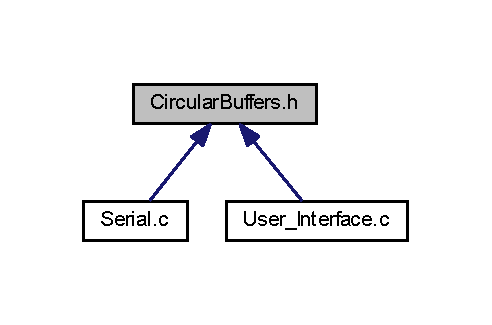
\includegraphics[width=236pt]{_circular_buffers_8h__dep__incl}
\end{center}
\end{figure}
\subsection*{Data Structures}
\begin{DoxyCompactItemize}
\item 
struct \hyperlink{structcircular_buffer}{circular\+Buffer}
\end{DoxyCompactItemize}
\subsection*{Macros}
\begin{DoxyCompactItemize}
\item 
\#define \hyperlink{_circular_buffers_8h_ac70e6264441e929fe13460353eb275c8}{inc\+Mod}(ptr)~if(ptr==\hyperlink{_circular_buffers_8h_a5a69f707d5405fe875b322c6bfbace46}{B\+U\+F\+F\+E\+R\+L\+E\+N\+G\+T\+H}-\/1) ptr = 0; else ptr++;
\item 
\#define \hyperlink{_circular_buffers_8h_aeabcb3d395f687162520f9f72c926edf}{empty}(buf)~(buf.\+tail == buf.\+head)
\item 
\#define \hyperlink{_circular_buffers_8h_a380cd5dd5680e22e1b6d839a57781661}{full}(buf)~(buf.\+head == (buf.\+tail + 1) \% \hyperlink{_circular_buffers_8h_a5a69f707d5405fe875b322c6bfbace46}{B\+U\+F\+F\+E\+R\+L\+E\+N\+G\+T\+H})
\item 
\#define \hyperlink{_circular_buffers_8h_ab6770f937bcc348970693cd84824bf9f}{peek}(buf)~buf.\+data\mbox{[}buf.\+head\mbox{]}
\item 
\#define \hyperlink{_circular_buffers_8h_aba30707c86c50590824a646a3ef26fbb}{push}(byte, buf)~buf.\+data\mbox{[}buf.\+tail\mbox{]} = byte; if(\hyperlink{_circular_buffers_8h_a380cd5dd5680e22e1b6d839a57781661}{full}(buf)) \hyperlink{_circular_buffers_8h_ac70e6264441e929fe13460353eb275c8}{inc\+Mod}(buf.\+head); \hyperlink{_circular_buffers_8h_ac70e6264441e929fe13460353eb275c8}{inc\+Mod}(buf.\+tail)
\item 
\#define \hyperlink{_circular_buffers_8h_aea34ae72df51f27dbb0562f5d9a23de0}{pop}(buf)~buf.\+data\mbox{[}buf.\+head\mbox{]}; if (!\hyperlink{_circular_buffers_8h_aeabcb3d395f687162520f9f72c926edf}{empty}(buf)) \hyperlink{_circular_buffers_8h_ac70e6264441e929fe13460353eb275c8}{inc\+Mod}(buf.\+head)
\item 
\#define \hyperlink{_circular_buffers_8h_a526002aa17fac30d010d4d7315d5d81c}{init}(buf)~buf.\+tail = 0; buf.\+head = 0
\item 
\#define \hyperlink{_circular_buffers_8h_a5a69f707d5405fe875b322c6bfbace46}{B\+U\+F\+F\+E\+R\+L\+E\+N\+G\+T\+H}~30
\item 
\#define \hyperlink{_circular_buffers_8h_a6e3f4516c9290cae3eaa13d167d5b6fe}{B\+U\+F\+F\+E\+R\+S\+\_\+\+H}~0
\end{DoxyCompactItemize}


\subsection{Macro Definition Documentation}
\hypertarget{_circular_buffers_8h_a5a69f707d5405fe875b322c6bfbace46}{\index{Circular\+Buffers.\+h@{Circular\+Buffers.\+h}!B\+U\+F\+F\+E\+R\+L\+E\+N\+G\+T\+H@{B\+U\+F\+F\+E\+R\+L\+E\+N\+G\+T\+H}}
\index{B\+U\+F\+F\+E\+R\+L\+E\+N\+G\+T\+H@{B\+U\+F\+F\+E\+R\+L\+E\+N\+G\+T\+H}!Circular\+Buffers.\+h@{Circular\+Buffers.\+h}}
\subsubsection[{B\+U\+F\+F\+E\+R\+L\+E\+N\+G\+T\+H}]{\setlength{\rightskip}{0pt plus 5cm}\#define B\+U\+F\+F\+E\+R\+L\+E\+N\+G\+T\+H~30}}\label{_circular_buffers_8h_a5a69f707d5405fe875b322c6bfbace46}


Definition at line 24 of file Circular\+Buffers.\+h.

\hypertarget{_circular_buffers_8h_a6e3f4516c9290cae3eaa13d167d5b6fe}{\index{Circular\+Buffers.\+h@{Circular\+Buffers.\+h}!B\+U\+F\+F\+E\+R\+S\+\_\+\+H@{B\+U\+F\+F\+E\+R\+S\+\_\+\+H}}
\index{B\+U\+F\+F\+E\+R\+S\+\_\+\+H@{B\+U\+F\+F\+E\+R\+S\+\_\+\+H}!Circular\+Buffers.\+h@{Circular\+Buffers.\+h}}
\subsubsection[{B\+U\+F\+F\+E\+R\+S\+\_\+\+H}]{\setlength{\rightskip}{0pt plus 5cm}\#define B\+U\+F\+F\+E\+R\+S\+\_\+\+H~0}}\label{_circular_buffers_8h_a6e3f4516c9290cae3eaa13d167d5b6fe}


Definition at line 34 of file Circular\+Buffers.\+h.

\hypertarget{_circular_buffers_8h_aeabcb3d395f687162520f9f72c926edf}{\index{Circular\+Buffers.\+h@{Circular\+Buffers.\+h}!empty@{empty}}
\index{empty@{empty}!Circular\+Buffers.\+h@{Circular\+Buffers.\+h}}
\subsubsection[{empty}]{\setlength{\rightskip}{0pt plus 5cm}\#define empty(
\begin{DoxyParamCaption}
\item[{}]{buf}
\end{DoxyParamCaption}
)~(buf.\+tail == buf.\+head)}}\label{_circular_buffers_8h_aeabcb3d395f687162520f9f72c926edf}


Definition at line 15 of file Circular\+Buffers.\+h.

\hypertarget{_circular_buffers_8h_a380cd5dd5680e22e1b6d839a57781661}{\index{Circular\+Buffers.\+h@{Circular\+Buffers.\+h}!full@{full}}
\index{full@{full}!Circular\+Buffers.\+h@{Circular\+Buffers.\+h}}
\subsubsection[{full}]{\setlength{\rightskip}{0pt plus 5cm}\#define full(
\begin{DoxyParamCaption}
\item[{}]{buf}
\end{DoxyParamCaption}
)~(buf.\+head == (buf.\+tail + 1) \% {\bf B\+U\+F\+F\+E\+R\+L\+E\+N\+G\+T\+H})}}\label{_circular_buffers_8h_a380cd5dd5680e22e1b6d839a57781661}


Definition at line 16 of file Circular\+Buffers.\+h.

\hypertarget{_circular_buffers_8h_ac70e6264441e929fe13460353eb275c8}{\index{Circular\+Buffers.\+h@{Circular\+Buffers.\+h}!inc\+Mod@{inc\+Mod}}
\index{inc\+Mod@{inc\+Mod}!Circular\+Buffers.\+h@{Circular\+Buffers.\+h}}
\subsubsection[{inc\+Mod}]{\setlength{\rightskip}{0pt plus 5cm}\#define inc\+Mod(
\begin{DoxyParamCaption}
\item[{}]{ptr}
\end{DoxyParamCaption}
)~if(ptr=={\bf B\+U\+F\+F\+E\+R\+L\+E\+N\+G\+T\+H}-\/1) ptr = 0; else ptr++;}}\label{_circular_buffers_8h_ac70e6264441e929fe13460353eb275c8}


Definition at line 14 of file Circular\+Buffers.\+h.

\hypertarget{_circular_buffers_8h_a526002aa17fac30d010d4d7315d5d81c}{\index{Circular\+Buffers.\+h@{Circular\+Buffers.\+h}!init@{init}}
\index{init@{init}!Circular\+Buffers.\+h@{Circular\+Buffers.\+h}}
\subsubsection[{init}]{\setlength{\rightskip}{0pt plus 5cm}\#define init(
\begin{DoxyParamCaption}
\item[{}]{buf}
\end{DoxyParamCaption}
)~buf.\+tail = 0; buf.\+head = 0}}\label{_circular_buffers_8h_a526002aa17fac30d010d4d7315d5d81c}


Definition at line 21 of file Circular\+Buffers.\+h.

\hypertarget{_circular_buffers_8h_ab6770f937bcc348970693cd84824bf9f}{\index{Circular\+Buffers.\+h@{Circular\+Buffers.\+h}!peek@{peek}}
\index{peek@{peek}!Circular\+Buffers.\+h@{Circular\+Buffers.\+h}}
\subsubsection[{peek}]{\setlength{\rightskip}{0pt plus 5cm}\#define peek(
\begin{DoxyParamCaption}
\item[{}]{buf}
\end{DoxyParamCaption}
)~buf.\+data\mbox{[}buf.\+head\mbox{]}}}\label{_circular_buffers_8h_ab6770f937bcc348970693cd84824bf9f}


Definition at line 17 of file Circular\+Buffers.\+h.

\hypertarget{_circular_buffers_8h_aea34ae72df51f27dbb0562f5d9a23de0}{\index{Circular\+Buffers.\+h@{Circular\+Buffers.\+h}!pop@{pop}}
\index{pop@{pop}!Circular\+Buffers.\+h@{Circular\+Buffers.\+h}}
\subsubsection[{pop}]{\setlength{\rightskip}{0pt plus 5cm}\#define pop(
\begin{DoxyParamCaption}
\item[{}]{buf}
\end{DoxyParamCaption}
)~buf.\+data\mbox{[}buf.\+head\mbox{]}; if (!{\bf empty}(buf)) {\bf inc\+Mod}(buf.\+head)}}\label{_circular_buffers_8h_aea34ae72df51f27dbb0562f5d9a23de0}


Definition at line 20 of file Circular\+Buffers.\+h.

\hypertarget{_circular_buffers_8h_aba30707c86c50590824a646a3ef26fbb}{\index{Circular\+Buffers.\+h@{Circular\+Buffers.\+h}!push@{push}}
\index{push@{push}!Circular\+Buffers.\+h@{Circular\+Buffers.\+h}}
\subsubsection[{push}]{\setlength{\rightskip}{0pt plus 5cm}\#define push(
\begin{DoxyParamCaption}
\item[{}]{byte, }
\item[{}]{buf}
\end{DoxyParamCaption}
)~buf.\+data\mbox{[}buf.\+tail\mbox{]} = byte; if({\bf full}(buf)) {\bf inc\+Mod}(buf.\+head); {\bf inc\+Mod}(buf.\+tail)}}\label{_circular_buffers_8h_aba30707c86c50590824a646a3ef26fbb}


Definition at line 19 of file Circular\+Buffers.\+h.


\hypertarget{_common_8h}{\section{Common.\+h File Reference}
\label{_common_8h}\index{Common.\+h@{Common.\+h}}
}
{\ttfamily \#include $<$stdio.\+h$>$}\\*
{\ttfamily \#include $<$stdlib.\+h$>$}\\*
{\ttfamily \#include $<$math.\+h$>$}\\*
{\ttfamily \#include $<$p18f4520.\+h$>$}\\*
{\ttfamily \#include $<$timers.\+h$>$}\\*
{\ttfamily \#include $<$adc.\+h$>$}\\*
{\ttfamily \#include $<$capture.\+h$>$}\\*
{\ttfamily \#include $<$usart.\+h$>$}\\*
{\ttfamily \#include $<$compare.\+h$>$}\\*
\subsection*{Data Structures}
\begin{DoxyCompactItemize}
\item 
struct \hyperlink{struct_direction}{Direction}
\item 
struct \hyperlink{struct_tracking_data}{Tracking\+Data}
\item 
struct \hyperlink{structsystem_state}{system\+State}
\end{DoxyCompactItemize}
\subsection*{Macros}
\begin{DoxyCompactItemize}
\item 
\#define \hyperlink{_common_8h_ad0d718ce41d188a939567abd92667796}{M\+N\+M\+L}
\item 
\#define \hyperlink{_common_8h_ad9fa804805fca2632643680804f7e911}{N\+E\+X\+T\+\_\+\+S\+T\+A\+T\+E}(s, state)~state.\+previous = state.\+current; state.\+current = s
\item 
\#define \hyperlink{_common_8h_a26a5416cb7bb43bd2f2eaaa7feaff84d}{N\+E\+X\+T\+\_\+\+S\+T\+A\+T\+E\+\_\+\+P\+T\+R}(s, state)~state-\/$>$previous = state-\/$>$current; state-\/$>$current = s
\item 
\#define \hyperlink{_common_8h_a4d6bb91285c504f7a5a882961cf405a9}{D\+I\+V\+\_\+2}(v)~((v) $>$$>$ 1)
\item 
\#define \hyperlink{_common_8h_abe112bea83dc5d8fb3a5a7ccc80b7abb}{D\+I\+V\+\_\+4}(v)~((v) $>$$>$ 2)
\item 
\#define \hyperlink{_common_8h_a4f978d22e3309b4121d0a95a74a1faba}{D\+I\+V\+\_\+8}(v)~((v) $>$$>$ 3)
\item 
\#define \hyperlink{_common_8h_aaf396e0300e6c0cd62ba67c6b6ab4bff}{D\+I\+V\+\_\+16}(v)~((v) $>$$>$ 4)
\item 
\#define \hyperlink{_common_8h_a6cd2ce042188839a264c5ba1627df97e}{D\+I\+V\+\_\+32}(v)~((v) $>$$>$ 5)
\item 
\#define \hyperlink{_common_8h_abcbec04588cd79b47e54f7259474e854}{D\+I\+V\+\_\+64}(v)~((v) $>$$>$ 6)
\item 
\#define \hyperlink{_common_8h_abdf4b624268c124f05cbb2954854f80c}{D\+I\+V\+\_\+128}(v)~((v) $>$$>$ 7)
\item 
\#define \hyperlink{_common_8h_ad36de0b0221fc009ad6b3a8671da028f}{D\+I\+V\+\_\+256}(v)~((v) $>$$>$ 8)
\item 
\#define \hyperlink{_common_8h_a6606c956e93ac0da035a298ec8073174}{D\+I\+V\+\_\+512}(v)~((v) $>$$>$ 9)
\item 
\#define \hyperlink{_common_8h_a740656a5f724d0a99e528def8ce50125}{D\+I\+V\+\_\+1024}(v)~((v) $>$$>$ 10)
\item 
\#define \hyperlink{_common_8h_a8d2e675fd4bbca53be91ffadf0c11673}{D\+I\+V\+\_\+4096}(v)~((v) $>$$>$ 12)
\item 
\#define \hyperlink{_common_8h_a9469c415aff989522dac534ab8adb35e}{D\+I\+V\+\_\+65536}(v)~((v) $>$$>$ 16)
\item 
\#define \hyperlink{_common_8h_a5d9d454d4b9f2ff8106d5199ac0d0186}{S\+W\+A\+P}(x, y)~(y = (y $^\wedge$ (x = (x $^\wedge$ (y = (x $^\wedge$ y))))))
\item 
\#define \hyperlink{_common_8h_a5b107d0db5d9abf4a7219b5d13d2c54e}{A\+D\+C\+\_\+\+I\+R\+\_\+\+R\+E\+A\+D}~0
\item 
\#define \hyperlink{_common_8h_a135151cc09e1094dbb0163c3d696e630}{A\+D\+C\+\_\+\+T\+E\+M\+P\+\_\+\+R\+E\+A\+D}~1
\item 
\#define \hyperlink{_common_8h_a1518840d35b90121383f93c00eba9164}{A\+D\+C\+\_\+\+D\+I\+A\+L\+\_\+\+R\+E\+A\+D}~2
\item 
\#define \hyperlink{_common_8h_aef3509d0d4bc8291df1b76f894a1e251}{T\+X\+\_\+\+I\+N\+T}~(\hyperlink{p18f4520_8h_a045c6555e7e82fcf68e608d4404fb9ed}{P\+I\+R1bits.\+T\+X\+I\+F} \&\& \hyperlink{p18f4520_8h_ae7b3b4752a0a4b6c084f1599ea98e724}{P\+I\+E1bits.\+T\+X\+I\+E})
\item 
\#define \hyperlink{_common_8h_a62ad39277340a9f95c1464e4a4b1b5a1}{R\+C\+\_\+\+I\+N\+T}~(\hyperlink{p18f4520_8h_a8ff1127552738fc483a7e1887045e8d2}{P\+I\+R1bits.\+R\+C\+I\+F} \&\& \hyperlink{p18f4520_8h_a756f5bf99764eb500a4a22b0693efb03}{P\+I\+E1bits.\+R\+C\+I\+E})
\item 
\#define \hyperlink{_common_8h_a1673a1a80febeafd51f3f02508a0ea71}{C\+C\+P1\+\_\+\+I\+N\+T}~(\hyperlink{p18f4520_8h_a6daa84b9e3f6496da3121a80506f444e}{P\+I\+R1bits.\+C\+C\+P1\+I\+F} \&\& \hyperlink{p18f4520_8h_a25d4adacdc481717b9c89f8352bc4bc6}{P\+I\+E1bits.\+C\+C\+P1\+I\+E})
\item 
\#define \hyperlink{_common_8h_aee2ef60613898be37c57266698616e33}{C\+C\+P2\+\_\+\+I\+N\+T}~(\hyperlink{p18f4520_8h_a7d689151681a8a50c953ecefd618eeb4}{P\+I\+R2bits.\+C\+C\+P2\+I\+F} \&\& \hyperlink{p18f4520_8h_af032cd1ef97761506102829f69feb189}{P\+I\+E2bits.\+C\+C\+P2\+I\+E})
\item 
\#define \hyperlink{_common_8h_ace4d61c3a12d8faab31305402fe1e074}{I\+N\+T0\+\_\+\+I\+N\+T}~(\hyperlink{p18f4520_8h_a9879ca934031776b77a0c19f1dce1b54}{I\+N\+T\+C\+O\+Nbits.\+I\+N\+T0\+I\+F} \&\& \hyperlink{p18f4520_8h_a35711f92541b36401c4a6a1575cb18ea}{I\+N\+T\+C\+O\+Nbits.\+I\+N\+T0\+I\+E})
\item 
\#define \hyperlink{_common_8h_afeb5099420bb15f8f59a24c3426de8f1}{R\+B\+\_\+\+I\+N\+T}~(\hyperlink{p18f4520_8h_ad8f6df4237b4615b8389534a9bd451da}{I\+N\+T\+C\+O\+Nbits.\+R\+B\+I\+F} \&\& \hyperlink{p18f4520_8h_ab20cb587b32c351a91e1b912ce3e29f4}{I\+N\+T\+C\+O\+Nbits.\+R\+B\+I\+E})
\item 
\#define \hyperlink{_common_8h_af6baae9385e65b47397c25f253cd8893}{T\+M\+R2\+\_\+\+I\+N\+T}~(\hyperlink{p18f4520_8h_a3e1791e78ad5d0e6b89e44e50c74f2c6}{P\+I\+R1bits.\+T\+M\+R2\+I\+F} \&\& \hyperlink{p18f4520_8h_a2616057e89e17857a0232b45825b8a4a}{P\+I\+E1bits.\+T\+M\+R2\+I\+E})
\item 
\#define \hyperlink{_common_8h_a5d4ee5c980131f617eac819f887ccff8}{T\+M\+R0\+\_\+\+I\+N\+T}~(\hyperlink{p18f4520_8h_a0301f42bbd887e533352a52d65e0f73d}{I\+N\+T\+C\+O\+Nbits.\+T\+M\+R0\+I\+F} \&\& \hyperlink{p18f4520_8h_aa9618f14f6542a5dac7d44cf1d7e1023}{I\+N\+T\+C\+O\+Nbits.\+T\+M\+R0\+I\+E})
\item 
\#define \hyperlink{_common_8h_af1b5f2499fdbb5b83800325b12a062cf}{T\+M\+R1\+\_\+\+I\+N\+T}~(\hyperlink{p18f4520_8h_a1ca0d1f4b314bcc9d4a42d92d4512118}{P\+I\+R1bits.\+T\+M\+R1\+I\+F} \&\& \hyperlink{p18f4520_8h_a41b95c767b7f4f9d788d421633333f25}{P\+I\+E1bits.\+T\+M\+R1\+I\+E})
\item 
\#define \hyperlink{_common_8h_a37a3fed60a18eefca9f30c8929272a35}{T\+M\+R3\+\_\+\+I\+N\+T}~(\hyperlink{p18f4520_8h_a3543e05a68f8aaf308e3abf391109a47}{P\+I\+R2bits.\+T\+M\+R3\+I\+F} \&\& \hyperlink{p18f4520_8h_a0f9cc64ee6e86633138b4e186eae33e2}{P\+I\+E2bits.\+T\+M\+R3\+I\+E})
\item 
\#define \hyperlink{_common_8h_ae19ae26fb5206ab6d949596d972ca430}{A\+D\+C\+\_\+\+I\+N\+T}~(\hyperlink{p18f4520_8h_aca1613e7087914be4d69c5770eb8f4a3}{P\+I\+R1bits.\+A\+D\+I\+F} \&\& \hyperlink{p18f4520_8h_ace69098082b2fd1d0929e31e71c1d5a9}{P\+I\+E1bits.\+A\+D\+I\+E})
\item 
\#define \hyperlink{_common_8h_a2fa3b4c4837187612ff9b0236d0d705f}{S\+S\+P\+\_\+\+I\+N\+T}~(\hyperlink{p18f4520_8h_a8001253a95878a1eab217642803eb655}{P\+I\+R1bits.\+S\+S\+P\+I\+F} \&\& \hyperlink{p18f4520_8h_acf24cc2186d69e72711aea0c30b99228}{P\+I\+E1bits.\+S\+S\+P\+I\+E})
\item 
\#define \hyperlink{_common_8h_ad9822079fd16e03a52bf566ce3fe221c}{B\+C\+L\+\_\+\+I\+N\+T}~(\hyperlink{p18f4520_8h_a903514afa08123232b8209785a448348}{P\+I\+R2bits.\+B\+C\+L\+I\+F} \&\& \hyperlink{p18f4520_8h_aae975fe98fee9b9a8c3beaa9964bbc8f}{P\+I\+E2bits.\+B\+C\+L\+I\+E})
\item 
\#define \hyperlink{_common_8h_ab3771f37588656c8d037de34edf2a88f}{L\+V\+D\+\_\+\+I\+N\+T}~(\hyperlink{p18f4520_8h_a7eed8d56af8d3063c286adba368d8dff}{P\+I\+R2bits.\+L\+V\+D\+I\+F} \&\& \hyperlink{p18f4520_8h_a957b8cf8198b7ca9c30cf9c730960a94}{P\+I\+E2bits.\+L\+V\+D\+I\+E})
\item 
\#define \hyperlink{_common_8h_ae8aa3ab3a23a388dab62ac86ee5e2545}{C\+C\+P1\+\_\+\+C\+L\+E\+A\+R}~(\hyperlink{p18f4520_8h_a6daa84b9e3f6496da3121a80506f444e}{P\+I\+R1bits.\+C\+C\+P1\+I\+F} = 0)
\item 
\#define \hyperlink{_common_8h_a4e461245300e8ea7e5c6af0741a33855}{C\+C\+P2\+\_\+\+C\+L\+E\+A\+R}~(\hyperlink{p18f4520_8h_a7d689151681a8a50c953ecefd618eeb4}{P\+I\+R2bits.\+C\+C\+P2\+I\+F} = 0)
\item 
\#define \hyperlink{_common_8h_a3be7ef61d339af381862a81d4b363efb}{C\+L\+O\+C\+K}~10000000
\item 
\#define \hyperlink{_common_8h_a644329678dec72e39b8847963e59c35d}{F\+O\+S\+C\+\_\+4}~2500000
\end{DoxyCompactItemize}
\subsection*{Enumerations}
\begin{DoxyCompactItemize}
\item 
enum \hyperlink{_common_8h_a2db986326a654991cce9b1c2b1670677}{Target\+State} \{ \\*
\hyperlink{_common_8h_a2db986326a654991cce9b1c2b1670677aba1240809f7ca0c3eb4ee13d2abe47e2}{N\+O\+\_\+\+T\+A\+R\+G\+E\+T}, 
\hyperlink{_common_8h_a2db986326a654991cce9b1c2b1670677a02f92f801598d94c6fd997546781a275}{O\+U\+T\+\_\+\+O\+F\+\_\+\+I\+R}, 
\hyperlink{_common_8h_a2db986326a654991cce9b1c2b1670677a49a975d06b51d93badc62d5685898851}{B\+A\+D\+\_\+\+D\+I\+R}, 
\hyperlink{_common_8h_a2db986326a654991cce9b1c2b1670677a4e09a3b8626706bec6e8b94f8e43007f}{G\+O\+O\+D\+\_\+\+T\+R\+A\+C\+K}, 
\\*
\hyperlink{_common_8h_a2db986326a654991cce9b1c2b1670677a1095d17ed354ef770b301c64f7b09262}{C\+L\+O\+S\+E\+\_\+\+R\+A\+N\+G\+E}
 \}
\item 
enum \hyperlink{_common_8h_a05931287b056487cf89495f39026fbe1}{possible\+\_\+states} \{ \hyperlink{_common_8h_a05931287b056487cf89495f39026fbe1a632fa39438c1676b435ec43e6a0f9647}{U\+N\+D\+E\+F}, 
\hyperlink{_common_8h_a05931287b056487cf89495f39026fbe1a0cb1b2c6a7db1f1084886c98909a3f36}{I\+N\+I\+T}, 
\hyperlink{_common_8h_a05931287b056487cf89495f39026fbe1a6e8623178c4e7a9db6aed4db75f8bd07}{S\+R\+C\+H}, 
\hyperlink{_common_8h_a05931287b056487cf89495f39026fbe1a70ca1afd3ed8312624a30c3993afc279}{T\+R\+C\+K}
 \}
\end{DoxyCompactItemize}


\subsection{Macro Definition Documentation}
\hypertarget{_common_8h_a1518840d35b90121383f93c00eba9164}{\index{Common.\+h@{Common.\+h}!A\+D\+C\+\_\+\+D\+I\+A\+L\+\_\+\+R\+E\+A\+D@{A\+D\+C\+\_\+\+D\+I\+A\+L\+\_\+\+R\+E\+A\+D}}
\index{A\+D\+C\+\_\+\+D\+I\+A\+L\+\_\+\+R\+E\+A\+D@{A\+D\+C\+\_\+\+D\+I\+A\+L\+\_\+\+R\+E\+A\+D}!Common.\+h@{Common.\+h}}
\subsubsection[{A\+D\+C\+\_\+\+D\+I\+A\+L\+\_\+\+R\+E\+A\+D}]{\setlength{\rightskip}{0pt plus 5cm}\#define A\+D\+C\+\_\+\+D\+I\+A\+L\+\_\+\+R\+E\+A\+D~2}}\label{_common_8h_a1518840d35b90121383f93c00eba9164}


Definition at line 88 of file Common.\+h.

\hypertarget{_common_8h_ae19ae26fb5206ab6d949596d972ca430}{\index{Common.\+h@{Common.\+h}!A\+D\+C\+\_\+\+I\+N\+T@{A\+D\+C\+\_\+\+I\+N\+T}}
\index{A\+D\+C\+\_\+\+I\+N\+T@{A\+D\+C\+\_\+\+I\+N\+T}!Common.\+h@{Common.\+h}}
\subsubsection[{A\+D\+C\+\_\+\+I\+N\+T}]{\setlength{\rightskip}{0pt plus 5cm}\#define A\+D\+C\+\_\+\+I\+N\+T~({\bf P\+I\+R1bits.\+A\+D\+I\+F} \&\& {\bf P\+I\+E1bits.\+A\+D\+I\+E})}}\label{_common_8h_ae19ae26fb5206ab6d949596d972ca430}


Definition at line 102 of file Common.\+h.

\hypertarget{_common_8h_a5b107d0db5d9abf4a7219b5d13d2c54e}{\index{Common.\+h@{Common.\+h}!A\+D\+C\+\_\+\+I\+R\+\_\+\+R\+E\+A\+D@{A\+D\+C\+\_\+\+I\+R\+\_\+\+R\+E\+A\+D}}
\index{A\+D\+C\+\_\+\+I\+R\+\_\+\+R\+E\+A\+D@{A\+D\+C\+\_\+\+I\+R\+\_\+\+R\+E\+A\+D}!Common.\+h@{Common.\+h}}
\subsubsection[{A\+D\+C\+\_\+\+I\+R\+\_\+\+R\+E\+A\+D}]{\setlength{\rightskip}{0pt plus 5cm}\#define A\+D\+C\+\_\+\+I\+R\+\_\+\+R\+E\+A\+D~0}}\label{_common_8h_a5b107d0db5d9abf4a7219b5d13d2c54e}


Definition at line 86 of file Common.\+h.

\hypertarget{_common_8h_a135151cc09e1094dbb0163c3d696e630}{\index{Common.\+h@{Common.\+h}!A\+D\+C\+\_\+\+T\+E\+M\+P\+\_\+\+R\+E\+A\+D@{A\+D\+C\+\_\+\+T\+E\+M\+P\+\_\+\+R\+E\+A\+D}}
\index{A\+D\+C\+\_\+\+T\+E\+M\+P\+\_\+\+R\+E\+A\+D@{A\+D\+C\+\_\+\+T\+E\+M\+P\+\_\+\+R\+E\+A\+D}!Common.\+h@{Common.\+h}}
\subsubsection[{A\+D\+C\+\_\+\+T\+E\+M\+P\+\_\+\+R\+E\+A\+D}]{\setlength{\rightskip}{0pt plus 5cm}\#define A\+D\+C\+\_\+\+T\+E\+M\+P\+\_\+\+R\+E\+A\+D~1}}\label{_common_8h_a135151cc09e1094dbb0163c3d696e630}


Definition at line 87 of file Common.\+h.

\hypertarget{_common_8h_ad9822079fd16e03a52bf566ce3fe221c}{\index{Common.\+h@{Common.\+h}!B\+C\+L\+\_\+\+I\+N\+T@{B\+C\+L\+\_\+\+I\+N\+T}}
\index{B\+C\+L\+\_\+\+I\+N\+T@{B\+C\+L\+\_\+\+I\+N\+T}!Common.\+h@{Common.\+h}}
\subsubsection[{B\+C\+L\+\_\+\+I\+N\+T}]{\setlength{\rightskip}{0pt plus 5cm}\#define B\+C\+L\+\_\+\+I\+N\+T~({\bf P\+I\+R2bits.\+B\+C\+L\+I\+F} \&\& {\bf P\+I\+E2bits.\+B\+C\+L\+I\+E})}}\label{_common_8h_ad9822079fd16e03a52bf566ce3fe221c}


Definition at line 104 of file Common.\+h.

\hypertarget{_common_8h_ae8aa3ab3a23a388dab62ac86ee5e2545}{\index{Common.\+h@{Common.\+h}!C\+C\+P1\+\_\+\+C\+L\+E\+A\+R@{C\+C\+P1\+\_\+\+C\+L\+E\+A\+R}}
\index{C\+C\+P1\+\_\+\+C\+L\+E\+A\+R@{C\+C\+P1\+\_\+\+C\+L\+E\+A\+R}!Common.\+h@{Common.\+h}}
\subsubsection[{C\+C\+P1\+\_\+\+C\+L\+E\+A\+R}]{\setlength{\rightskip}{0pt plus 5cm}\#define C\+C\+P1\+\_\+\+C\+L\+E\+A\+R~({\bf P\+I\+R1bits.\+C\+C\+P1\+I\+F} = 0)}}\label{_common_8h_ae8aa3ab3a23a388dab62ac86ee5e2545}


Definition at line 107 of file Common.\+h.

\hypertarget{_common_8h_a1673a1a80febeafd51f3f02508a0ea71}{\index{Common.\+h@{Common.\+h}!C\+C\+P1\+\_\+\+I\+N\+T@{C\+C\+P1\+\_\+\+I\+N\+T}}
\index{C\+C\+P1\+\_\+\+I\+N\+T@{C\+C\+P1\+\_\+\+I\+N\+T}!Common.\+h@{Common.\+h}}
\subsubsection[{C\+C\+P1\+\_\+\+I\+N\+T}]{\setlength{\rightskip}{0pt plus 5cm}\#define C\+C\+P1\+\_\+\+I\+N\+T~({\bf P\+I\+R1bits.\+C\+C\+P1\+I\+F} \&\& {\bf P\+I\+E1bits.\+C\+C\+P1\+I\+E})}}\label{_common_8h_a1673a1a80febeafd51f3f02508a0ea71}


Definition at line 93 of file Common.\+h.

\hypertarget{_common_8h_a4e461245300e8ea7e5c6af0741a33855}{\index{Common.\+h@{Common.\+h}!C\+C\+P2\+\_\+\+C\+L\+E\+A\+R@{C\+C\+P2\+\_\+\+C\+L\+E\+A\+R}}
\index{C\+C\+P2\+\_\+\+C\+L\+E\+A\+R@{C\+C\+P2\+\_\+\+C\+L\+E\+A\+R}!Common.\+h@{Common.\+h}}
\subsubsection[{C\+C\+P2\+\_\+\+C\+L\+E\+A\+R}]{\setlength{\rightskip}{0pt plus 5cm}\#define C\+C\+P2\+\_\+\+C\+L\+E\+A\+R~({\bf P\+I\+R2bits.\+C\+C\+P2\+I\+F} = 0)}}\label{_common_8h_a4e461245300e8ea7e5c6af0741a33855}


Definition at line 108 of file Common.\+h.

\hypertarget{_common_8h_aee2ef60613898be37c57266698616e33}{\index{Common.\+h@{Common.\+h}!C\+C\+P2\+\_\+\+I\+N\+T@{C\+C\+P2\+\_\+\+I\+N\+T}}
\index{C\+C\+P2\+\_\+\+I\+N\+T@{C\+C\+P2\+\_\+\+I\+N\+T}!Common.\+h@{Common.\+h}}
\subsubsection[{C\+C\+P2\+\_\+\+I\+N\+T}]{\setlength{\rightskip}{0pt plus 5cm}\#define C\+C\+P2\+\_\+\+I\+N\+T~({\bf P\+I\+R2bits.\+C\+C\+P2\+I\+F} \&\& {\bf P\+I\+E2bits.\+C\+C\+P2\+I\+E})}}\label{_common_8h_aee2ef60613898be37c57266698616e33}


Definition at line 94 of file Common.\+h.

\hypertarget{_common_8h_a3be7ef61d339af381862a81d4b363efb}{\index{Common.\+h@{Common.\+h}!C\+L\+O\+C\+K@{C\+L\+O\+C\+K}}
\index{C\+L\+O\+C\+K@{C\+L\+O\+C\+K}!Common.\+h@{Common.\+h}}
\subsubsection[{C\+L\+O\+C\+K}]{\setlength{\rightskip}{0pt plus 5cm}\#define C\+L\+O\+C\+K~10000000}}\label{_common_8h_a3be7ef61d339af381862a81d4b363efb}


Definition at line 111 of file Common.\+h.

\hypertarget{_common_8h_a740656a5f724d0a99e528def8ce50125}{\index{Common.\+h@{Common.\+h}!D\+I\+V\+\_\+1024@{D\+I\+V\+\_\+1024}}
\index{D\+I\+V\+\_\+1024@{D\+I\+V\+\_\+1024}!Common.\+h@{Common.\+h}}
\subsubsection[{D\+I\+V\+\_\+1024}]{\setlength{\rightskip}{0pt plus 5cm}\#define D\+I\+V\+\_\+1024(
\begin{DoxyParamCaption}
\item[{}]{v}
\end{DoxyParamCaption}
)~((v) $>$$>$ 10)}}\label{_common_8h_a740656a5f724d0a99e528def8ce50125}


Definition at line 79 of file Common.\+h.

\hypertarget{_common_8h_abdf4b624268c124f05cbb2954854f80c}{\index{Common.\+h@{Common.\+h}!D\+I\+V\+\_\+128@{D\+I\+V\+\_\+128}}
\index{D\+I\+V\+\_\+128@{D\+I\+V\+\_\+128}!Common.\+h@{Common.\+h}}
\subsubsection[{D\+I\+V\+\_\+128}]{\setlength{\rightskip}{0pt plus 5cm}\#define D\+I\+V\+\_\+128(
\begin{DoxyParamCaption}
\item[{}]{v}
\end{DoxyParamCaption}
)~((v) $>$$>$ 7)}}\label{_common_8h_abdf4b624268c124f05cbb2954854f80c}


Definition at line 76 of file Common.\+h.

\hypertarget{_common_8h_aaf396e0300e6c0cd62ba67c6b6ab4bff}{\index{Common.\+h@{Common.\+h}!D\+I\+V\+\_\+16@{D\+I\+V\+\_\+16}}
\index{D\+I\+V\+\_\+16@{D\+I\+V\+\_\+16}!Common.\+h@{Common.\+h}}
\subsubsection[{D\+I\+V\+\_\+16}]{\setlength{\rightskip}{0pt plus 5cm}\#define D\+I\+V\+\_\+16(
\begin{DoxyParamCaption}
\item[{}]{v}
\end{DoxyParamCaption}
)~((v) $>$$>$ 4)}}\label{_common_8h_aaf396e0300e6c0cd62ba67c6b6ab4bff}


Definition at line 73 of file Common.\+h.

\hypertarget{_common_8h_a4d6bb91285c504f7a5a882961cf405a9}{\index{Common.\+h@{Common.\+h}!D\+I\+V\+\_\+2@{D\+I\+V\+\_\+2}}
\index{D\+I\+V\+\_\+2@{D\+I\+V\+\_\+2}!Common.\+h@{Common.\+h}}
\subsubsection[{D\+I\+V\+\_\+2}]{\setlength{\rightskip}{0pt plus 5cm}\#define D\+I\+V\+\_\+2(
\begin{DoxyParamCaption}
\item[{}]{v}
\end{DoxyParamCaption}
)~((v) $>$$>$ 1)}}\label{_common_8h_a4d6bb91285c504f7a5a882961cf405a9}


Definition at line 70 of file Common.\+h.

\hypertarget{_common_8h_ad36de0b0221fc009ad6b3a8671da028f}{\index{Common.\+h@{Common.\+h}!D\+I\+V\+\_\+256@{D\+I\+V\+\_\+256}}
\index{D\+I\+V\+\_\+256@{D\+I\+V\+\_\+256}!Common.\+h@{Common.\+h}}
\subsubsection[{D\+I\+V\+\_\+256}]{\setlength{\rightskip}{0pt plus 5cm}\#define D\+I\+V\+\_\+256(
\begin{DoxyParamCaption}
\item[{}]{v}
\end{DoxyParamCaption}
)~((v) $>$$>$ 8)}}\label{_common_8h_ad36de0b0221fc009ad6b3a8671da028f}


Definition at line 77 of file Common.\+h.

\hypertarget{_common_8h_a6cd2ce042188839a264c5ba1627df97e}{\index{Common.\+h@{Common.\+h}!D\+I\+V\+\_\+32@{D\+I\+V\+\_\+32}}
\index{D\+I\+V\+\_\+32@{D\+I\+V\+\_\+32}!Common.\+h@{Common.\+h}}
\subsubsection[{D\+I\+V\+\_\+32}]{\setlength{\rightskip}{0pt plus 5cm}\#define D\+I\+V\+\_\+32(
\begin{DoxyParamCaption}
\item[{}]{v}
\end{DoxyParamCaption}
)~((v) $>$$>$ 5)}}\label{_common_8h_a6cd2ce042188839a264c5ba1627df97e}


Definition at line 74 of file Common.\+h.

\hypertarget{_common_8h_abe112bea83dc5d8fb3a5a7ccc80b7abb}{\index{Common.\+h@{Common.\+h}!D\+I\+V\+\_\+4@{D\+I\+V\+\_\+4}}
\index{D\+I\+V\+\_\+4@{D\+I\+V\+\_\+4}!Common.\+h@{Common.\+h}}
\subsubsection[{D\+I\+V\+\_\+4}]{\setlength{\rightskip}{0pt plus 5cm}\#define D\+I\+V\+\_\+4(
\begin{DoxyParamCaption}
\item[{}]{v}
\end{DoxyParamCaption}
)~((v) $>$$>$ 2)}}\label{_common_8h_abe112bea83dc5d8fb3a5a7ccc80b7abb}


Definition at line 71 of file Common.\+h.

\hypertarget{_common_8h_a8d2e675fd4bbca53be91ffadf0c11673}{\index{Common.\+h@{Common.\+h}!D\+I\+V\+\_\+4096@{D\+I\+V\+\_\+4096}}
\index{D\+I\+V\+\_\+4096@{D\+I\+V\+\_\+4096}!Common.\+h@{Common.\+h}}
\subsubsection[{D\+I\+V\+\_\+4096}]{\setlength{\rightskip}{0pt plus 5cm}\#define D\+I\+V\+\_\+4096(
\begin{DoxyParamCaption}
\item[{}]{v}
\end{DoxyParamCaption}
)~((v) $>$$>$ 12)}}\label{_common_8h_a8d2e675fd4bbca53be91ffadf0c11673}


Definition at line 80 of file Common.\+h.

\hypertarget{_common_8h_a6606c956e93ac0da035a298ec8073174}{\index{Common.\+h@{Common.\+h}!D\+I\+V\+\_\+512@{D\+I\+V\+\_\+512}}
\index{D\+I\+V\+\_\+512@{D\+I\+V\+\_\+512}!Common.\+h@{Common.\+h}}
\subsubsection[{D\+I\+V\+\_\+512}]{\setlength{\rightskip}{0pt plus 5cm}\#define D\+I\+V\+\_\+512(
\begin{DoxyParamCaption}
\item[{}]{v}
\end{DoxyParamCaption}
)~((v) $>$$>$ 9)}}\label{_common_8h_a6606c956e93ac0da035a298ec8073174}


Definition at line 78 of file Common.\+h.

\hypertarget{_common_8h_abcbec04588cd79b47e54f7259474e854}{\index{Common.\+h@{Common.\+h}!D\+I\+V\+\_\+64@{D\+I\+V\+\_\+64}}
\index{D\+I\+V\+\_\+64@{D\+I\+V\+\_\+64}!Common.\+h@{Common.\+h}}
\subsubsection[{D\+I\+V\+\_\+64}]{\setlength{\rightskip}{0pt plus 5cm}\#define D\+I\+V\+\_\+64(
\begin{DoxyParamCaption}
\item[{}]{v}
\end{DoxyParamCaption}
)~((v) $>$$>$ 6)}}\label{_common_8h_abcbec04588cd79b47e54f7259474e854}


Definition at line 75 of file Common.\+h.

\hypertarget{_common_8h_a9469c415aff989522dac534ab8adb35e}{\index{Common.\+h@{Common.\+h}!D\+I\+V\+\_\+65536@{D\+I\+V\+\_\+65536}}
\index{D\+I\+V\+\_\+65536@{D\+I\+V\+\_\+65536}!Common.\+h@{Common.\+h}}
\subsubsection[{D\+I\+V\+\_\+65536}]{\setlength{\rightskip}{0pt plus 5cm}\#define D\+I\+V\+\_\+65536(
\begin{DoxyParamCaption}
\item[{}]{v}
\end{DoxyParamCaption}
)~((v) $>$$>$ 16)}}\label{_common_8h_a9469c415aff989522dac534ab8adb35e}


Definition at line 81 of file Common.\+h.

\hypertarget{_common_8h_a4f978d22e3309b4121d0a95a74a1faba}{\index{Common.\+h@{Common.\+h}!D\+I\+V\+\_\+8@{D\+I\+V\+\_\+8}}
\index{D\+I\+V\+\_\+8@{D\+I\+V\+\_\+8}!Common.\+h@{Common.\+h}}
\subsubsection[{D\+I\+V\+\_\+8}]{\setlength{\rightskip}{0pt plus 5cm}\#define D\+I\+V\+\_\+8(
\begin{DoxyParamCaption}
\item[{}]{v}
\end{DoxyParamCaption}
)~((v) $>$$>$ 3)}}\label{_common_8h_a4f978d22e3309b4121d0a95a74a1faba}


Definition at line 72 of file Common.\+h.

\hypertarget{_common_8h_a644329678dec72e39b8847963e59c35d}{\index{Common.\+h@{Common.\+h}!F\+O\+S\+C\+\_\+4@{F\+O\+S\+C\+\_\+4}}
\index{F\+O\+S\+C\+\_\+4@{F\+O\+S\+C\+\_\+4}!Common.\+h@{Common.\+h}}
\subsubsection[{F\+O\+S\+C\+\_\+4}]{\setlength{\rightskip}{0pt plus 5cm}\#define F\+O\+S\+C\+\_\+4~2500000}}\label{_common_8h_a644329678dec72e39b8847963e59c35d}


Definition at line 112 of file Common.\+h.

\hypertarget{_common_8h_ace4d61c3a12d8faab31305402fe1e074}{\index{Common.\+h@{Common.\+h}!I\+N\+T0\+\_\+\+I\+N\+T@{I\+N\+T0\+\_\+\+I\+N\+T}}
\index{I\+N\+T0\+\_\+\+I\+N\+T@{I\+N\+T0\+\_\+\+I\+N\+T}!Common.\+h@{Common.\+h}}
\subsubsection[{I\+N\+T0\+\_\+\+I\+N\+T}]{\setlength{\rightskip}{0pt plus 5cm}\#define I\+N\+T0\+\_\+\+I\+N\+T~({\bf I\+N\+T\+C\+O\+Nbits.\+I\+N\+T0\+I\+F} \&\& {\bf I\+N\+T\+C\+O\+Nbits.\+I\+N\+T0\+I\+E})}}\label{_common_8h_ace4d61c3a12d8faab31305402fe1e074}


Definition at line 95 of file Common.\+h.

\hypertarget{_common_8h_ab3771f37588656c8d037de34edf2a88f}{\index{Common.\+h@{Common.\+h}!L\+V\+D\+\_\+\+I\+N\+T@{L\+V\+D\+\_\+\+I\+N\+T}}
\index{L\+V\+D\+\_\+\+I\+N\+T@{L\+V\+D\+\_\+\+I\+N\+T}!Common.\+h@{Common.\+h}}
\subsubsection[{L\+V\+D\+\_\+\+I\+N\+T}]{\setlength{\rightskip}{0pt plus 5cm}\#define L\+V\+D\+\_\+\+I\+N\+T~({\bf P\+I\+R2bits.\+L\+V\+D\+I\+F} \&\& {\bf P\+I\+E2bits.\+L\+V\+D\+I\+E})}}\label{_common_8h_ab3771f37588656c8d037de34edf2a88f}


Definition at line 105 of file Common.\+h.

\hypertarget{_common_8h_ad0d718ce41d188a939567abd92667796}{\index{Common.\+h@{Common.\+h}!M\+N\+M\+L@{M\+N\+M\+L}}
\index{M\+N\+M\+L@{M\+N\+M\+L}!Common.\+h@{Common.\+h}}
\subsubsection[{M\+N\+M\+L}]{\setlength{\rightskip}{0pt plus 5cm}\#define M\+N\+M\+L}}\label{_common_8h_ad0d718ce41d188a939567abd92667796}


Definition at line 9 of file Common.\+h.

\hypertarget{_common_8h_ad9fa804805fca2632643680804f7e911}{\index{Common.\+h@{Common.\+h}!N\+E\+X\+T\+\_\+\+S\+T\+A\+T\+E@{N\+E\+X\+T\+\_\+\+S\+T\+A\+T\+E}}
\index{N\+E\+X\+T\+\_\+\+S\+T\+A\+T\+E@{N\+E\+X\+T\+\_\+\+S\+T\+A\+T\+E}!Common.\+h@{Common.\+h}}
\subsubsection[{N\+E\+X\+T\+\_\+\+S\+T\+A\+T\+E}]{\setlength{\rightskip}{0pt plus 5cm}\#define N\+E\+X\+T\+\_\+\+S\+T\+A\+T\+E(
\begin{DoxyParamCaption}
\item[{}]{s, }
\item[{}]{state}
\end{DoxyParamCaption}
)~state.\+previous = state.\+current; state.\+current = s}}\label{_common_8h_ad9fa804805fca2632643680804f7e911}


Definition at line 59 of file Common.\+h.

\hypertarget{_common_8h_a26a5416cb7bb43bd2f2eaaa7feaff84d}{\index{Common.\+h@{Common.\+h}!N\+E\+X\+T\+\_\+\+S\+T\+A\+T\+E\+\_\+\+P\+T\+R@{N\+E\+X\+T\+\_\+\+S\+T\+A\+T\+E\+\_\+\+P\+T\+R}}
\index{N\+E\+X\+T\+\_\+\+S\+T\+A\+T\+E\+\_\+\+P\+T\+R@{N\+E\+X\+T\+\_\+\+S\+T\+A\+T\+E\+\_\+\+P\+T\+R}!Common.\+h@{Common.\+h}}
\subsubsection[{N\+E\+X\+T\+\_\+\+S\+T\+A\+T\+E\+\_\+\+P\+T\+R}]{\setlength{\rightskip}{0pt plus 5cm}\#define N\+E\+X\+T\+\_\+\+S\+T\+A\+T\+E\+\_\+\+P\+T\+R(
\begin{DoxyParamCaption}
\item[{}]{s, }
\item[{}]{state}
\end{DoxyParamCaption}
)~state-\/$>$previous = state-\/$>$current; state-\/$>$current = s}}\label{_common_8h_a26a5416cb7bb43bd2f2eaaa7feaff84d}


Definition at line 60 of file Common.\+h.

\hypertarget{_common_8h_afeb5099420bb15f8f59a24c3426de8f1}{\index{Common.\+h@{Common.\+h}!R\+B\+\_\+\+I\+N\+T@{R\+B\+\_\+\+I\+N\+T}}
\index{R\+B\+\_\+\+I\+N\+T@{R\+B\+\_\+\+I\+N\+T}!Common.\+h@{Common.\+h}}
\subsubsection[{R\+B\+\_\+\+I\+N\+T}]{\setlength{\rightskip}{0pt plus 5cm}\#define R\+B\+\_\+\+I\+N\+T~({\bf I\+N\+T\+C\+O\+Nbits.\+R\+B\+I\+F} \&\& {\bf I\+N\+T\+C\+O\+Nbits.\+R\+B\+I\+E})}}\label{_common_8h_afeb5099420bb15f8f59a24c3426de8f1}


Definition at line 96 of file Common.\+h.

\hypertarget{_common_8h_a62ad39277340a9f95c1464e4a4b1b5a1}{\index{Common.\+h@{Common.\+h}!R\+C\+\_\+\+I\+N\+T@{R\+C\+\_\+\+I\+N\+T}}
\index{R\+C\+\_\+\+I\+N\+T@{R\+C\+\_\+\+I\+N\+T}!Common.\+h@{Common.\+h}}
\subsubsection[{R\+C\+\_\+\+I\+N\+T}]{\setlength{\rightskip}{0pt plus 5cm}\#define R\+C\+\_\+\+I\+N\+T~({\bf P\+I\+R1bits.\+R\+C\+I\+F} \&\& {\bf P\+I\+E1bits.\+R\+C\+I\+E})}}\label{_common_8h_a62ad39277340a9f95c1464e4a4b1b5a1}


Definition at line 92 of file Common.\+h.

\hypertarget{_common_8h_a2fa3b4c4837187612ff9b0236d0d705f}{\index{Common.\+h@{Common.\+h}!S\+S\+P\+\_\+\+I\+N\+T@{S\+S\+P\+\_\+\+I\+N\+T}}
\index{S\+S\+P\+\_\+\+I\+N\+T@{S\+S\+P\+\_\+\+I\+N\+T}!Common.\+h@{Common.\+h}}
\subsubsection[{S\+S\+P\+\_\+\+I\+N\+T}]{\setlength{\rightskip}{0pt plus 5cm}\#define S\+S\+P\+\_\+\+I\+N\+T~({\bf P\+I\+R1bits.\+S\+S\+P\+I\+F} \&\& {\bf P\+I\+E1bits.\+S\+S\+P\+I\+E})}}\label{_common_8h_a2fa3b4c4837187612ff9b0236d0d705f}


Definition at line 103 of file Common.\+h.

\hypertarget{_common_8h_a5d9d454d4b9f2ff8106d5199ac0d0186}{\index{Common.\+h@{Common.\+h}!S\+W\+A\+P@{S\+W\+A\+P}}
\index{S\+W\+A\+P@{S\+W\+A\+P}!Common.\+h@{Common.\+h}}
\subsubsection[{S\+W\+A\+P}]{\setlength{\rightskip}{0pt plus 5cm}\#define S\+W\+A\+P(
\begin{DoxyParamCaption}
\item[{}]{x, }
\item[{}]{y}
\end{DoxyParamCaption}
)~(y = (y $^\wedge$ (x = (x $^\wedge$ (y = (x $^\wedge$ y))))))}}\label{_common_8h_a5d9d454d4b9f2ff8106d5199ac0d0186}


Definition at line 83 of file Common.\+h.

\hypertarget{_common_8h_a5d4ee5c980131f617eac819f887ccff8}{\index{Common.\+h@{Common.\+h}!T\+M\+R0\+\_\+\+I\+N\+T@{T\+M\+R0\+\_\+\+I\+N\+T}}
\index{T\+M\+R0\+\_\+\+I\+N\+T@{T\+M\+R0\+\_\+\+I\+N\+T}!Common.\+h@{Common.\+h}}
\subsubsection[{T\+M\+R0\+\_\+\+I\+N\+T}]{\setlength{\rightskip}{0pt plus 5cm}\#define T\+M\+R0\+\_\+\+I\+N\+T~({\bf I\+N\+T\+C\+O\+Nbits.\+T\+M\+R0\+I\+F} \&\& {\bf I\+N\+T\+C\+O\+Nbits.\+T\+M\+R0\+I\+E})}}\label{_common_8h_a5d4ee5c980131f617eac819f887ccff8}


Definition at line 99 of file Common.\+h.

\hypertarget{_common_8h_af1b5f2499fdbb5b83800325b12a062cf}{\index{Common.\+h@{Common.\+h}!T\+M\+R1\+\_\+\+I\+N\+T@{T\+M\+R1\+\_\+\+I\+N\+T}}
\index{T\+M\+R1\+\_\+\+I\+N\+T@{T\+M\+R1\+\_\+\+I\+N\+T}!Common.\+h@{Common.\+h}}
\subsubsection[{T\+M\+R1\+\_\+\+I\+N\+T}]{\setlength{\rightskip}{0pt plus 5cm}\#define T\+M\+R1\+\_\+\+I\+N\+T~({\bf P\+I\+R1bits.\+T\+M\+R1\+I\+F} \&\& {\bf P\+I\+E1bits.\+T\+M\+R1\+I\+E})}}\label{_common_8h_af1b5f2499fdbb5b83800325b12a062cf}


Definition at line 100 of file Common.\+h.

\hypertarget{_common_8h_af6baae9385e65b47397c25f253cd8893}{\index{Common.\+h@{Common.\+h}!T\+M\+R2\+\_\+\+I\+N\+T@{T\+M\+R2\+\_\+\+I\+N\+T}}
\index{T\+M\+R2\+\_\+\+I\+N\+T@{T\+M\+R2\+\_\+\+I\+N\+T}!Common.\+h@{Common.\+h}}
\subsubsection[{T\+M\+R2\+\_\+\+I\+N\+T}]{\setlength{\rightskip}{0pt plus 5cm}\#define T\+M\+R2\+\_\+\+I\+N\+T~({\bf P\+I\+R1bits.\+T\+M\+R2\+I\+F} \&\& {\bf P\+I\+E1bits.\+T\+M\+R2\+I\+E})}}\label{_common_8h_af6baae9385e65b47397c25f253cd8893}


Definition at line 97 of file Common.\+h.

\hypertarget{_common_8h_a37a3fed60a18eefca9f30c8929272a35}{\index{Common.\+h@{Common.\+h}!T\+M\+R3\+\_\+\+I\+N\+T@{T\+M\+R3\+\_\+\+I\+N\+T}}
\index{T\+M\+R3\+\_\+\+I\+N\+T@{T\+M\+R3\+\_\+\+I\+N\+T}!Common.\+h@{Common.\+h}}
\subsubsection[{T\+M\+R3\+\_\+\+I\+N\+T}]{\setlength{\rightskip}{0pt plus 5cm}\#define T\+M\+R3\+\_\+\+I\+N\+T~({\bf P\+I\+R2bits.\+T\+M\+R3\+I\+F} \&\& {\bf P\+I\+E2bits.\+T\+M\+R3\+I\+E})}}\label{_common_8h_a37a3fed60a18eefca9f30c8929272a35}


Definition at line 101 of file Common.\+h.

\hypertarget{_common_8h_aef3509d0d4bc8291df1b76f894a1e251}{\index{Common.\+h@{Common.\+h}!T\+X\+\_\+\+I\+N\+T@{T\+X\+\_\+\+I\+N\+T}}
\index{T\+X\+\_\+\+I\+N\+T@{T\+X\+\_\+\+I\+N\+T}!Common.\+h@{Common.\+h}}
\subsubsection[{T\+X\+\_\+\+I\+N\+T}]{\setlength{\rightskip}{0pt plus 5cm}\#define T\+X\+\_\+\+I\+N\+T~({\bf P\+I\+R1bits.\+T\+X\+I\+F} \&\& {\bf P\+I\+E1bits.\+T\+X\+I\+E})}}\label{_common_8h_aef3509d0d4bc8291df1b76f894a1e251}


Definition at line 91 of file Common.\+h.



\subsection{Enumeration Type Documentation}
\hypertarget{_common_8h_a05931287b056487cf89495f39026fbe1}{\index{Common.\+h@{Common.\+h}!possible\+\_\+states@{possible\+\_\+states}}
\index{possible\+\_\+states@{possible\+\_\+states}!Common.\+h@{Common.\+h}}
\subsubsection[{possible\+\_\+states}]{\setlength{\rightskip}{0pt plus 5cm}enum {\bf possible\+\_\+states}}}\label{_common_8h_a05931287b056487cf89495f39026fbe1}
\begin{Desc}
\item[Enumerator]\par
\begin{description}
\index{U\+N\+D\+E\+F@{U\+N\+D\+E\+F}!Common.\+h@{Common.\+h}}\index{Common.\+h@{Common.\+h}!U\+N\+D\+E\+F@{U\+N\+D\+E\+F}}\item[{\em 
\hypertarget{_common_8h_a05931287b056487cf89495f39026fbe1a632fa39438c1676b435ec43e6a0f9647}{U\+N\+D\+E\+F}\label{_common_8h_a05931287b056487cf89495f39026fbe1a632fa39438c1676b435ec43e6a0f9647}
}]\index{I\+N\+I\+T@{I\+N\+I\+T}!Common.\+h@{Common.\+h}}\index{Common.\+h@{Common.\+h}!I\+N\+I\+T@{I\+N\+I\+T}}\item[{\em 
\hypertarget{_common_8h_a05931287b056487cf89495f39026fbe1a0cb1b2c6a7db1f1084886c98909a3f36}{I\+N\+I\+T}\label{_common_8h_a05931287b056487cf89495f39026fbe1a0cb1b2c6a7db1f1084886c98909a3f36}
}]\index{S\+R\+C\+H@{S\+R\+C\+H}!Common.\+h@{Common.\+h}}\index{Common.\+h@{Common.\+h}!S\+R\+C\+H@{S\+R\+C\+H}}\item[{\em 
\hypertarget{_common_8h_a05931287b056487cf89495f39026fbe1a6e8623178c4e7a9db6aed4db75f8bd07}{S\+R\+C\+H}\label{_common_8h_a05931287b056487cf89495f39026fbe1a6e8623178c4e7a9db6aed4db75f8bd07}
}]\index{T\+R\+C\+K@{T\+R\+C\+K}!Common.\+h@{Common.\+h}}\index{Common.\+h@{Common.\+h}!T\+R\+C\+K@{T\+R\+C\+K}}\item[{\em 
\hypertarget{_common_8h_a05931287b056487cf89495f39026fbe1a70ca1afd3ed8312624a30c3993afc279}{T\+R\+C\+K}\label{_common_8h_a05931287b056487cf89495f39026fbe1a70ca1afd3ed8312624a30c3993afc279}
}]\end{description}
\end{Desc}


Definition at line 63 of file Common.\+h.

\hypertarget{_common_8h_a2db986326a654991cce9b1c2b1670677}{\index{Common.\+h@{Common.\+h}!Target\+State@{Target\+State}}
\index{Target\+State@{Target\+State}!Common.\+h@{Common.\+h}}
\subsubsection[{Target\+State}]{\setlength{\rightskip}{0pt plus 5cm}enum {\bf Target\+State}}}\label{_common_8h_a2db986326a654991cce9b1c2b1670677}
\begin{Desc}
\item[Enumerator]\par
\begin{description}
\index{N\+O\+\_\+\+T\+A\+R\+G\+E\+T@{N\+O\+\_\+\+T\+A\+R\+G\+E\+T}!Common.\+h@{Common.\+h}}\index{Common.\+h@{Common.\+h}!N\+O\+\_\+\+T\+A\+R\+G\+E\+T@{N\+O\+\_\+\+T\+A\+R\+G\+E\+T}}\item[{\em 
\hypertarget{_common_8h_a2db986326a654991cce9b1c2b1670677aba1240809f7ca0c3eb4ee13d2abe47e2}{N\+O\+\_\+\+T\+A\+R\+G\+E\+T}\label{_common_8h_a2db986326a654991cce9b1c2b1670677aba1240809f7ca0c3eb4ee13d2abe47e2}
}]\index{O\+U\+T\+\_\+\+O\+F\+\_\+\+I\+R@{O\+U\+T\+\_\+\+O\+F\+\_\+\+I\+R}!Common.\+h@{Common.\+h}}\index{Common.\+h@{Common.\+h}!O\+U\+T\+\_\+\+O\+F\+\_\+\+I\+R@{O\+U\+T\+\_\+\+O\+F\+\_\+\+I\+R}}\item[{\em 
\hypertarget{_common_8h_a2db986326a654991cce9b1c2b1670677a02f92f801598d94c6fd997546781a275}{O\+U\+T\+\_\+\+O\+F\+\_\+\+I\+R}\label{_common_8h_a2db986326a654991cce9b1c2b1670677a02f92f801598d94c6fd997546781a275}
}]\index{B\+A\+D\+\_\+\+D\+I\+R@{B\+A\+D\+\_\+\+D\+I\+R}!Common.\+h@{Common.\+h}}\index{Common.\+h@{Common.\+h}!B\+A\+D\+\_\+\+D\+I\+R@{B\+A\+D\+\_\+\+D\+I\+R}}\item[{\em 
\hypertarget{_common_8h_a2db986326a654991cce9b1c2b1670677a49a975d06b51d93badc62d5685898851}{B\+A\+D\+\_\+\+D\+I\+R}\label{_common_8h_a2db986326a654991cce9b1c2b1670677a49a975d06b51d93badc62d5685898851}
}]\index{G\+O\+O\+D\+\_\+\+T\+R\+A\+C\+K@{G\+O\+O\+D\+\_\+\+T\+R\+A\+C\+K}!Common.\+h@{Common.\+h}}\index{Common.\+h@{Common.\+h}!G\+O\+O\+D\+\_\+\+T\+R\+A\+C\+K@{G\+O\+O\+D\+\_\+\+T\+R\+A\+C\+K}}\item[{\em 
\hypertarget{_common_8h_a2db986326a654991cce9b1c2b1670677a4e09a3b8626706bec6e8b94f8e43007f}{G\+O\+O\+D\+\_\+\+T\+R\+A\+C\+K}\label{_common_8h_a2db986326a654991cce9b1c2b1670677a4e09a3b8626706bec6e8b94f8e43007f}
}]\index{C\+L\+O\+S\+E\+\_\+\+R\+A\+N\+G\+E@{C\+L\+O\+S\+E\+\_\+\+R\+A\+N\+G\+E}!Common.\+h@{Common.\+h}}\index{Common.\+h@{Common.\+h}!C\+L\+O\+S\+E\+\_\+\+R\+A\+N\+G\+E@{C\+L\+O\+S\+E\+\_\+\+R\+A\+N\+G\+E}}\item[{\em 
\hypertarget{_common_8h_a2db986326a654991cce9b1c2b1670677a1095d17ed354ef770b301c64f7b09262}{C\+L\+O\+S\+E\+\_\+\+R\+A\+N\+G\+E}\label{_common_8h_a2db986326a654991cce9b1c2b1670677a1095d17ed354ef770b301c64f7b09262}
}]\end{description}
\end{Desc}


Definition at line 55 of file Common.\+h.


\hypertarget{_config_regs18f4520_8h}{\section{Config\+Regs18f4520.\+h File Reference}
\label{_config_regs18f4520_8h}\index{Config\+Regs18f4520.\+h@{Config\+Regs18f4520.\+h}}
}


Include file to set the Configuration Bits of a P\+I\+C18\+F4520.  


{\ttfamily \#include $<$p18cxxx.\+h$>$}\\*
Include dependency graph for Config\+Regs18f4520.\+h\+:\nopagebreak
\begin{figure}[H]
\begin{center}
\leavevmode
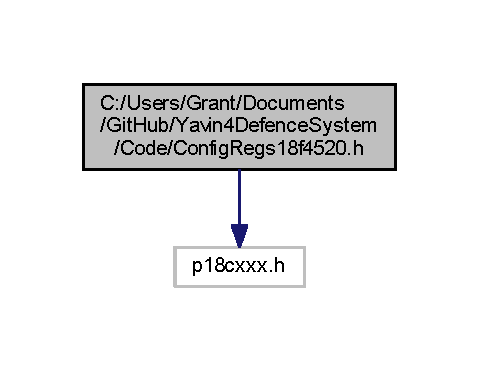
\includegraphics[width=188pt]{_config_regs18f4520_8h__incl}
\end{center}
\end{figure}


\subsection{Detailed Description}
Include file to set the Configuration Bits of a P\+I\+C18\+F4520. 

If the macro \+\_\+\+\_\+\+D\+E\+B\+U\+G is defined, the bits are set as appropriate for development and debugging\+:
\begin{DoxyItemize}
\item H\+S Oscillator; Oscillator Switch disabled; Power-\/\+On Timer;
\item Brown-\/out Reset disabled;
\item Watchdog Timer disabled;
\item C\+C\+P2 Multiplex disabled;
\item Stack Overflow Reset;
\item Low-\/voltage Programming disabled, Debug mode enabled;
\item No protection bits set.
\end{DoxyItemize}

If the macro \+\_\+\+\_\+\+D\+E\+B\+U\+G is N\+O\+T defined, the bits are set as appropriate for production code release\+:
\begin{DoxyItemize}
\item H\+S Oscillator; Oscillator Switch disabled; Power-\/\+On Timer;
\item Brown-\/out Reset enabled at 4.\+2\+V;
\item Watchdog Timer disabled;
\item C\+C\+P2 Multiplex disabled;
\item Stack Overflow Reset;
\item Low-\/voltage Programming and Debug mode disabled;
\item No protection bits set.
\end{DoxyItemize}

\begin{DoxyVersion}{Version}
0.\+1 -\/ derived from Config\+Regs18\+F452.\+h 
\end{DoxyVersion}
\begin{DoxyDate}{Date}
28-\/\+Aug-\/2014 
\end{DoxyDate}
\begin{DoxyAuthor}{Author}
David Rye
\end{DoxyAuthor}
\begin{DoxyNote}{Note}
This file was generated by the compiler from the command line\+: mcc18 -\/p18f4520 --help-\/config $>$ config\+Reg18\+F4520.\+h
\end{DoxyNote}
\begin{DoxyRefDesc}{Todo}
\item[\hyperlink{todo__todo000001}{Todo}]Consider if Watchdog Timer should be enabled for production code, and add W\+D\+T management code if so.\end{DoxyRefDesc}


\begin{DoxyRefDesc}{Todo}
\item[\hyperlink{todo__todo000002}{Todo}]Consider if Stack Overflow Reset should be enabled for production code. It may be better not to, as there is no re-\/entrant or recursive code, or dynamic memory allocation here -\/ if the code loads statically it should run.\end{DoxyRefDesc}


\begin{DoxyRefDesc}{Todo}
\item[\hyperlink{todo__todo000003}{Todo}]Change startup code c016iz.\+c so that everything (including initialised variables) correctly re-\/starts if \hyperlink{newmain_8c_acdef7a1fd863a6d3770c1268cb06add3}{main()} ever exits or a B\+O\+R or W\+D\+T reset occurs. \end{DoxyRefDesc}


Definition in file \hyperlink{_config_regs18f4520_8h_source}{Config\+Regs18f4520.\+h}.


\hypertarget{_interrupts_8c}{\section{Interrupts.\+c File Reference}
\label{_interrupts_8c}\index{Interrupts.\+c@{Interrupts.\+c}}
}
{\ttfamily \#include \char`\"{}Common.\+h\char`\"{}}\\*
{\ttfamily \#include \char`\"{}Tracking.\+h\char`\"{}}\\*
{\ttfamily \#include \char`\"{}Range.\+h\char`\"{}}\\*
{\ttfamily \#include \char`\"{}User\+\_\+\+Interface.\+h\char`\"{}}\\*
{\ttfamily \#include \char`\"{}Serial.\+h\char`\"{}}\\*
{\ttfamily \#include \char`\"{}Pan\+Tilt.\+h\char`\"{}}\\*
{\ttfamily \#include \char`\"{}Temp.\+h\char`\"{}}\\*
{\ttfamily \#include \char`\"{}Menusystem.\+h\char`\"{}}\\*
Include dependency graph for Interrupts.\+c\+:\nopagebreak
\begin{figure}[H]
\begin{center}
\leavevmode
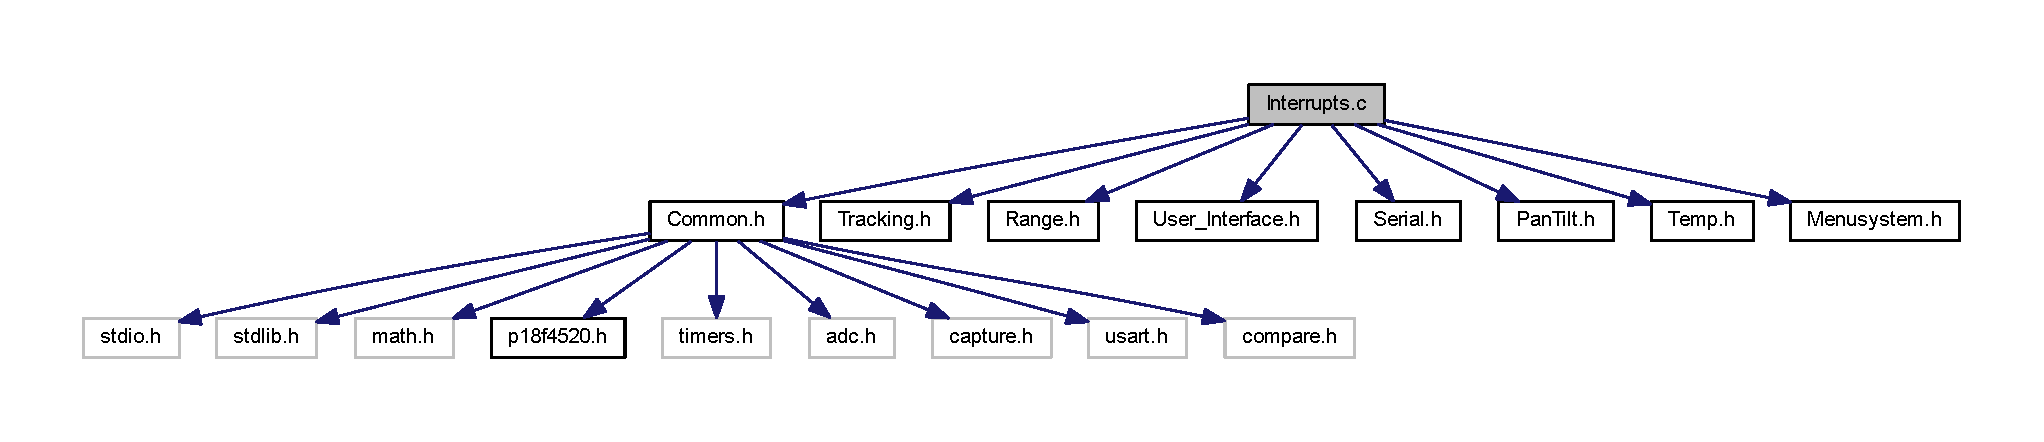
\includegraphics[width=350pt]{_interrupts_8c__incl}
\end{center}
\end{figure}
\subsection*{Functions}
\begin{DoxyCompactItemize}
\item 
void \hyperlink{_interrupts_8c_ac835f50b358d0d663df1b8b835f9bb87}{low\+I\+S\+R} (void)
\item 
void \hyperlink{_interrupts_8c_ae1ef1358e10604d046f54fc0b93c514c}{high\+I\+S\+R} (void)
\item 
void \hyperlink{_interrupts_8c_a6b8605436b00e1a9db52f2cb2094fdfd}{high\+Vector} (void)
\item 
void \hyperlink{_interrupts_8c_a0bf42af14e1d16197d7eb27ac5addca0}{low\+Vector} (void)
\end{DoxyCompactItemize}


\subsection{Function Documentation}
\hypertarget{_interrupts_8c_ae1ef1358e10604d046f54fc0b93c514c}{\index{Interrupts.\+c@{Interrupts.\+c}!high\+I\+S\+R@{high\+I\+S\+R}}
\index{high\+I\+S\+R@{high\+I\+S\+R}!Interrupts.\+c@{Interrupts.\+c}}
\subsubsection[{high\+I\+S\+R}]{\setlength{\rightskip}{0pt plus 5cm}void high\+I\+S\+R (
\begin{DoxyParamCaption}
\item[{void}]{}
\end{DoxyParamCaption}
)}}\label{_interrupts_8c_ae1ef1358e10604d046f54fc0b93c514c}


 Function\+: \hyperlink{_interrupts_8c_ae1ef1358e10604d046f54fc0b93c514c}{high\+I\+S\+R(void)}

Include\+: Local to \hyperlink{_interrupts_8c}{Interrupts.\+c}

Description\+: Interrupt Service Routine to check what condition initiated a high priority interrupt call, and perform the nessicary action

Arguments\+: None

Returns\+: None 

Definition at line 122 of file Interrupts.\+c.



Here is the call graph for this function\+:\nopagebreak
\begin{figure}[H]
\begin{center}
\leavevmode
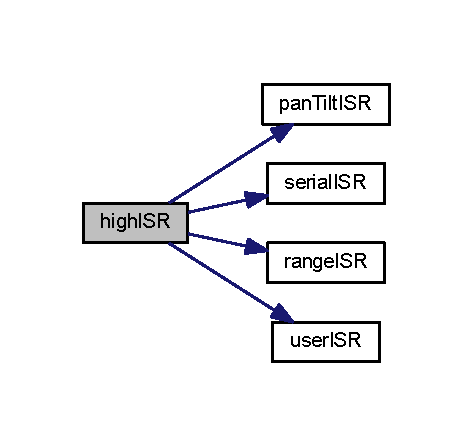
\includegraphics[width=227pt]{_interrupts_8c_ae1ef1358e10604d046f54fc0b93c514c_cgraph}
\end{center}
\end{figure}




Here is the caller graph for this function\+:\nopagebreak
\begin{figure}[H]
\begin{center}
\leavevmode
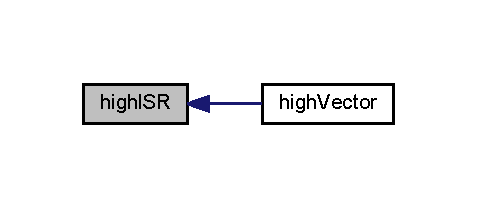
\includegraphics[width=229pt]{_interrupts_8c_ae1ef1358e10604d046f54fc0b93c514c_icgraph}
\end{center}
\end{figure}


\hypertarget{_interrupts_8c_a6b8605436b00e1a9db52f2cb2094fdfd}{\index{Interrupts.\+c@{Interrupts.\+c}!high\+Vector@{high\+Vector}}
\index{high\+Vector@{high\+Vector}!Interrupts.\+c@{Interrupts.\+c}}
\subsubsection[{high\+Vector}]{\setlength{\rightskip}{0pt plus 5cm}void high\+Vector (
\begin{DoxyParamCaption}
\item[{void}]{}
\end{DoxyParamCaption}
)}}\label{_interrupts_8c_a6b8605436b00e1a9db52f2cb2094fdfd}


 Function\+: \hyperlink{_interrupts_8c_a6b8605436b00e1a9db52f2cb2094fdfd}{high\+Vector(void)}

Include\+: Local to \hyperlink{_interrupts_8c}{Interrupts.\+c}

Description\+: Sends program control to the high priority I\+S\+R

Arguments\+: None

Returns\+: None

Remarks\+: This is an interrupt vector, placing a goto in the high priority interrupt table to call the high priority I\+S\+R 

Definition at line 50 of file Interrupts.\+c.



Here is the call graph for this function\+:\nopagebreak
\begin{figure}[H]
\begin{center}
\leavevmode
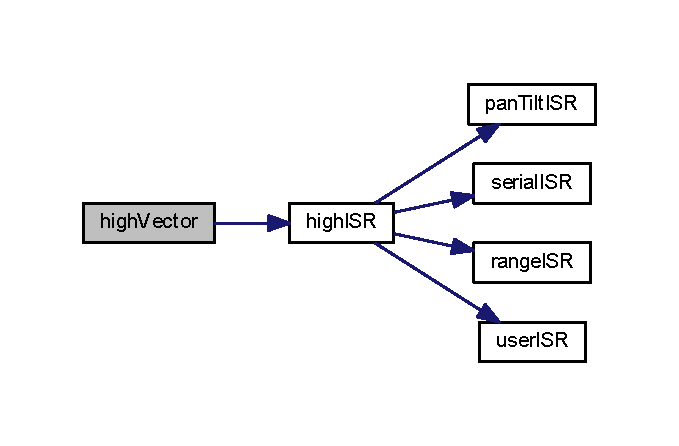
\includegraphics[width=326pt]{_interrupts_8c_a6b8605436b00e1a9db52f2cb2094fdfd_cgraph}
\end{center}
\end{figure}


\hypertarget{_interrupts_8c_ac835f50b358d0d663df1b8b835f9bb87}{\index{Interrupts.\+c@{Interrupts.\+c}!low\+I\+S\+R@{low\+I\+S\+R}}
\index{low\+I\+S\+R@{low\+I\+S\+R}!Interrupts.\+c@{Interrupts.\+c}}
\subsubsection[{low\+I\+S\+R}]{\setlength{\rightskip}{0pt plus 5cm}void low\+I\+S\+R (
\begin{DoxyParamCaption}
\item[{void}]{}
\end{DoxyParamCaption}
)}}\label{_interrupts_8c_ac835f50b358d0d663df1b8b835f9bb87}


 File\+: \hyperlink{_interrupts_8c}{Interrupts.\+c} Author\+: Grant

Description\+: Contains the interrupt service routines for the system.

Duties\+: -\/\+Handle all interrupts called by the system -\/\+Call relevant module service routines

Created on 8 October 2014, 11\+:27 A\+M



 Function\+: \hyperlink{_interrupts_8c_ac835f50b358d0d663df1b8b835f9bb87}{low\+I\+S\+R(void)}

Include\+: Local to \hyperlink{_interrupts_8c}{Interrupts.\+c}

Description\+: Interrupt Service Routine to check what condition initiated a low priority interrupt call, and perform the nessicary action

Arguments\+: None

Returns\+: None 

Definition at line 88 of file Interrupts.\+c.



Here is the call graph for this function\+:\nopagebreak
\begin{figure}[H]
\begin{center}
\leavevmode
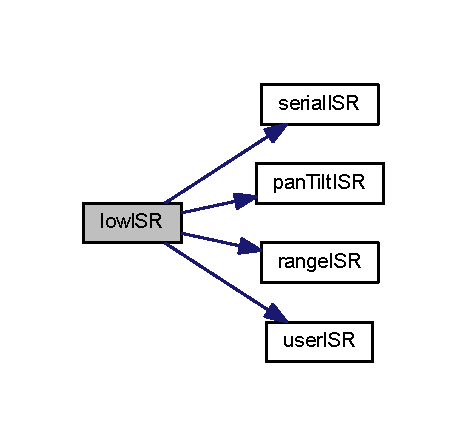
\includegraphics[width=224pt]{_interrupts_8c_ac835f50b358d0d663df1b8b835f9bb87_cgraph}
\end{center}
\end{figure}




Here is the caller graph for this function\+:\nopagebreak
\begin{figure}[H]
\begin{center}
\leavevmode
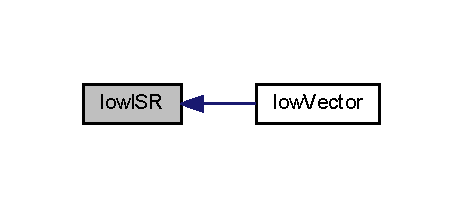
\includegraphics[width=222pt]{_interrupts_8c_ac835f50b358d0d663df1b8b835f9bb87_icgraph}
\end{center}
\end{figure}


\hypertarget{_interrupts_8c_a0bf42af14e1d16197d7eb27ac5addca0}{\index{Interrupts.\+c@{Interrupts.\+c}!low\+Vector@{low\+Vector}}
\index{low\+Vector@{low\+Vector}!Interrupts.\+c@{Interrupts.\+c}}
\subsubsection[{low\+Vector}]{\setlength{\rightskip}{0pt plus 5cm}void low\+Vector (
\begin{DoxyParamCaption}
\item[{void}]{}
\end{DoxyParamCaption}
)}}\label{_interrupts_8c_a0bf42af14e1d16197d7eb27ac5addca0}


 Function\+: \hyperlink{_interrupts_8c_a0bf42af14e1d16197d7eb27ac5addca0}{low\+Vector(void)}

Include\+: Local to \hyperlink{_interrupts_8c}{Interrupts.\+c}

Description\+: Sends program control to the low priority I\+S\+R

Arguments\+: None

Returns\+: None

Remarks\+: This is an interrupt vector, placing a goto in the low priority interrupt table to call the low priority I\+S\+R 

Definition at line 70 of file Interrupts.\+c.



Here is the call graph for this function\+:\nopagebreak
\begin{figure}[H]
\begin{center}
\leavevmode
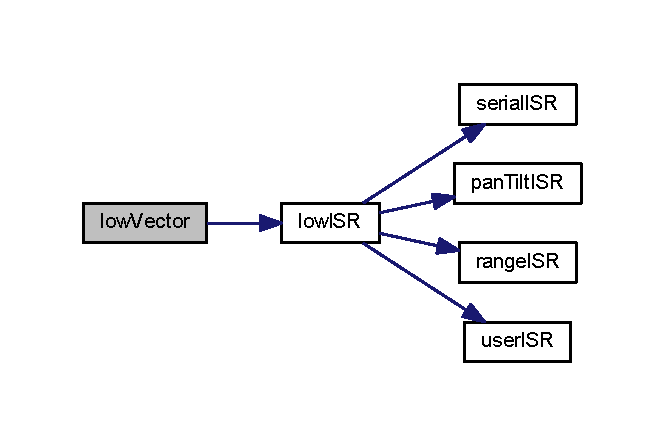
\includegraphics[width=319pt]{_interrupts_8c_a0bf42af14e1d16197d7eb27ac5addca0_cgraph}
\end{center}
\end{figure}



\hypertarget{_l_c_d_8c}{\section{L\+C\+D.\+c File Reference}
\label{_l_c_d_8c}\index{L\+C\+D.\+c@{L\+C\+D.\+c}}
}
{\ttfamily \#include \char`\"{}Common.\+h\char`\"{}}\\*
Include dependency graph for L\+C\+D.\+c\+:\nopagebreak
\begin{figure}[H]
\begin{center}
\leavevmode
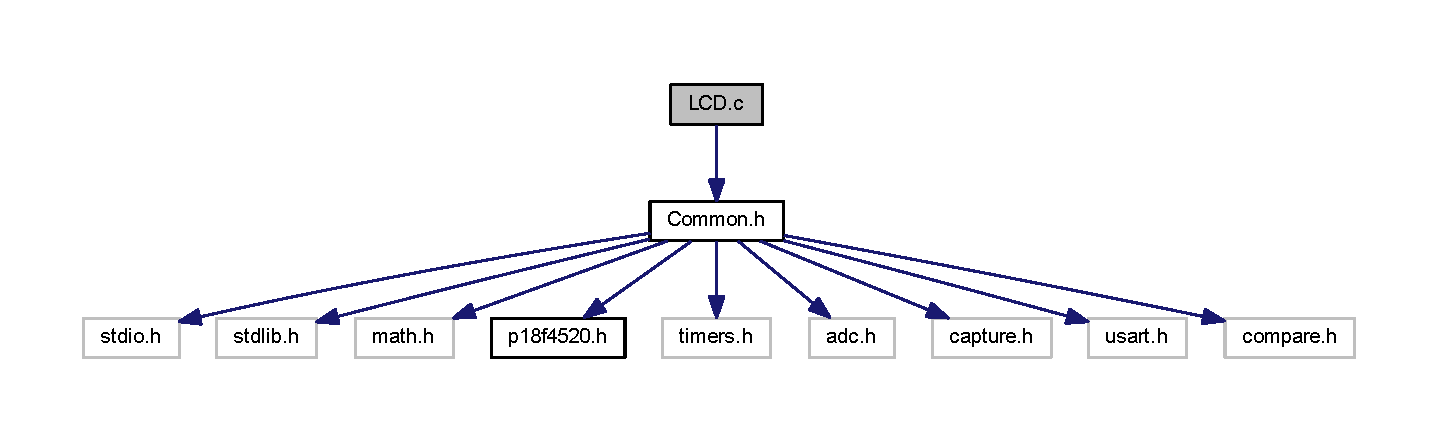
\includegraphics[width=350pt]{_l_c_d_8c__incl}
\end{center}
\end{figure}
\subsection*{Functions}
\begin{DoxyCompactItemize}
\item 
void \hyperlink{_l_c_d_8c_aaab6233be65b7399b3422eee9782508c}{config\+L\+C\+D} (void)
\item 
void \hyperlink{_l_c_d_8c_a8190804aeb1375a5a6b775f8e2b5d698}{display\+L\+C\+D} (char $\ast$string)
\end{DoxyCompactItemize}


\subsection{Function Documentation}
\hypertarget{_l_c_d_8c_aaab6233be65b7399b3422eee9782508c}{\index{L\+C\+D.\+c@{L\+C\+D.\+c}!config\+L\+C\+D@{config\+L\+C\+D}}
\index{config\+L\+C\+D@{config\+L\+C\+D}!L\+C\+D.\+c@{L\+C\+D.\+c}}
\subsubsection[{config\+L\+C\+D}]{\setlength{\rightskip}{0pt plus 5cm}void config\+L\+C\+D (
\begin{DoxyParamCaption}
\item[{void}]{}
\end{DoxyParamCaption}
)}}\label{_l_c_d_8c_aaab6233be65b7399b3422eee9782508c}


 File\+: \hyperlink{_user___interface_8c}{User\+\_\+\+Interface.\+c} Author\+: Grant

Description\+: Contains all the interface to the L\+C\+D hardware

Duties\+: -\/\+Interfaces with and controls the L\+C\+D -\/\+Displays data on the L\+C\+D

Created on 15 September 2014, 1\+:21 P\+M 

Definition at line 28 of file L\+C\+D.\+c.



Here is the caller graph for this function\+:\nopagebreak
\begin{figure}[H]
\begin{center}
\leavevmode
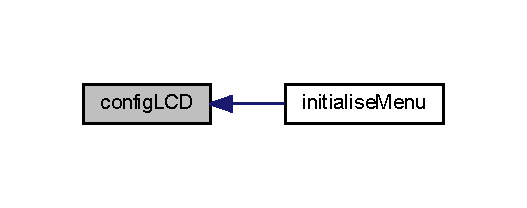
\includegraphics[width=253pt]{_l_c_d_8c_aaab6233be65b7399b3422eee9782508c_icgraph}
\end{center}
\end{figure}


\hypertarget{_l_c_d_8c_a8190804aeb1375a5a6b775f8e2b5d698}{\index{L\+C\+D.\+c@{L\+C\+D.\+c}!display\+L\+C\+D@{display\+L\+C\+D}}
\index{display\+L\+C\+D@{display\+L\+C\+D}!L\+C\+D.\+c@{L\+C\+D.\+c}}
\subsubsection[{display\+L\+C\+D}]{\setlength{\rightskip}{0pt plus 5cm}void display\+L\+C\+D (
\begin{DoxyParamCaption}
\item[{char $\ast$}]{string}
\end{DoxyParamCaption}
)}}\label{_l_c_d_8c_a8190804aeb1375a5a6b775f8e2b5d698}


 Function\+: \hyperlink{_l_c_d_8c_a8190804aeb1375a5a6b775f8e2b5d698}{display\+L\+C\+D(char $\ast$string)}

Include\+: \hyperlink{_l_c_d_8h}{L\+C\+D.\+h}

Description\+: Displays the given string on the L\+C\+D

Arguments\+: string -\/ pointer to the data to display

Returns\+: None 

Definition at line 44 of file L\+C\+D.\+c.


\hypertarget{_l_c_d_8h}{\section{L\+C\+D.\+h File Reference}
\label{_l_c_d_8h}\index{L\+C\+D.\+h@{L\+C\+D.\+h}}
}
This graph shows which files directly or indirectly include this file\+:
\nopagebreak
\begin{figure}[H]
\begin{center}
\leavevmode
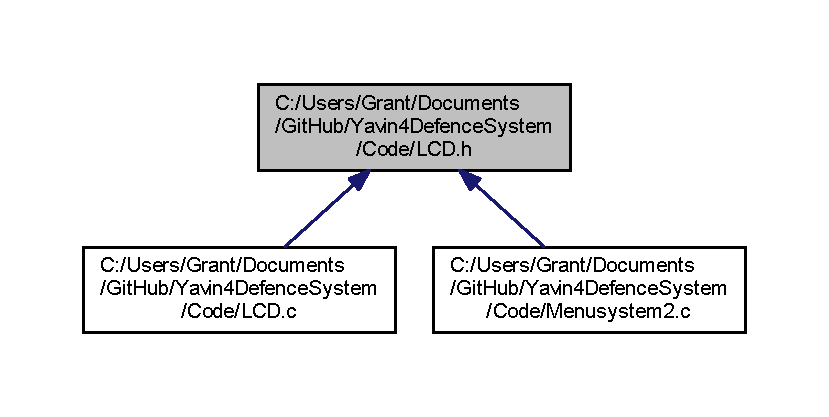
\includegraphics[width=166pt]{_l_c_d_8h__dep__incl}
\end{center}
\end{figure}
\subsection*{Functions}
\begin{DoxyCompactItemize}
\item 
void \hyperlink{_l_c_d_8h_aaab6233be65b7399b3422eee9782508c}{config\+L\+C\+D} (void)
\item 
void \hyperlink{_l_c_d_8h_a8190804aeb1375a5a6b775f8e2b5d698}{display\+L\+C\+D} (char $\ast$string)
\end{DoxyCompactItemize}


\subsection{Function Documentation}
\hypertarget{_l_c_d_8h_aaab6233be65b7399b3422eee9782508c}{\index{L\+C\+D.\+h@{L\+C\+D.\+h}!config\+L\+C\+D@{config\+L\+C\+D}}
\index{config\+L\+C\+D@{config\+L\+C\+D}!L\+C\+D.\+h@{L\+C\+D.\+h}}
\subsubsection[{config\+L\+C\+D}]{\setlength{\rightskip}{0pt plus 5cm}void config\+L\+C\+D (
\begin{DoxyParamCaption}
\item[{void}]{}
\end{DoxyParamCaption}
)}}\label{_l_c_d_8h_aaab6233be65b7399b3422eee9782508c}


Definition at line 23 of file L\+C\+D.\+c.



Here is the caller graph for this function\+:
\nopagebreak
\begin{figure}[H]
\begin{center}
\leavevmode
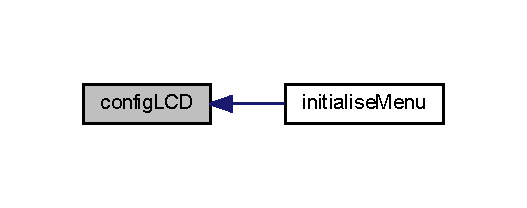
\includegraphics[width=253pt]{_l_c_d_8h_aaab6233be65b7399b3422eee9782508c_icgraph}
\end{center}
\end{figure}


\hypertarget{_l_c_d_8h_a8190804aeb1375a5a6b775f8e2b5d698}{\index{L\+C\+D.\+h@{L\+C\+D.\+h}!display\+L\+C\+D@{display\+L\+C\+D}}
\index{display\+L\+C\+D@{display\+L\+C\+D}!L\+C\+D.\+h@{L\+C\+D.\+h}}
\subsubsection[{display\+L\+C\+D}]{\setlength{\rightskip}{0pt plus 5cm}void display\+L\+C\+D (
\begin{DoxyParamCaption}
\item[{char $\ast$}]{string}
\end{DoxyParamCaption}
)}}\label{_l_c_d_8h_a8190804aeb1375a5a6b775f8e2b5d698}


 Function\+: \hyperlink{_l_c_d_8c_a8190804aeb1375a5a6b775f8e2b5d698}{display\+L\+C\+D(char $\ast$string)}

Include\+: \hyperlink{_l_c_d_8h}{L\+C\+D.\+h}

Description\+: Displays the given string on the L\+C\+D

Arguments\+: string -\/ pointer to the data to display

Returns\+: None 

Definition at line 39 of file L\+C\+D.\+c.


\hypertarget{_menusystem_8c}{\section{Menusystem.\+c File Reference}
\label{_menusystem_8c}\index{Menusystem.\+c@{Menusystem.\+c}}
}
{\ttfamily \#include \char`\"{}Common.\+h\char`\"{}}\\*
{\ttfamily \#include \char`\"{}Serial.\+h\char`\"{}}\\*
{\ttfamily \#include \char`\"{}User\+\_\+\+Interface.\+h\char`\"{}}\\*
Include dependency graph for Menusystem.\+c\+:
\nopagebreak
\begin{figure}[H]
\begin{center}
\leavevmode
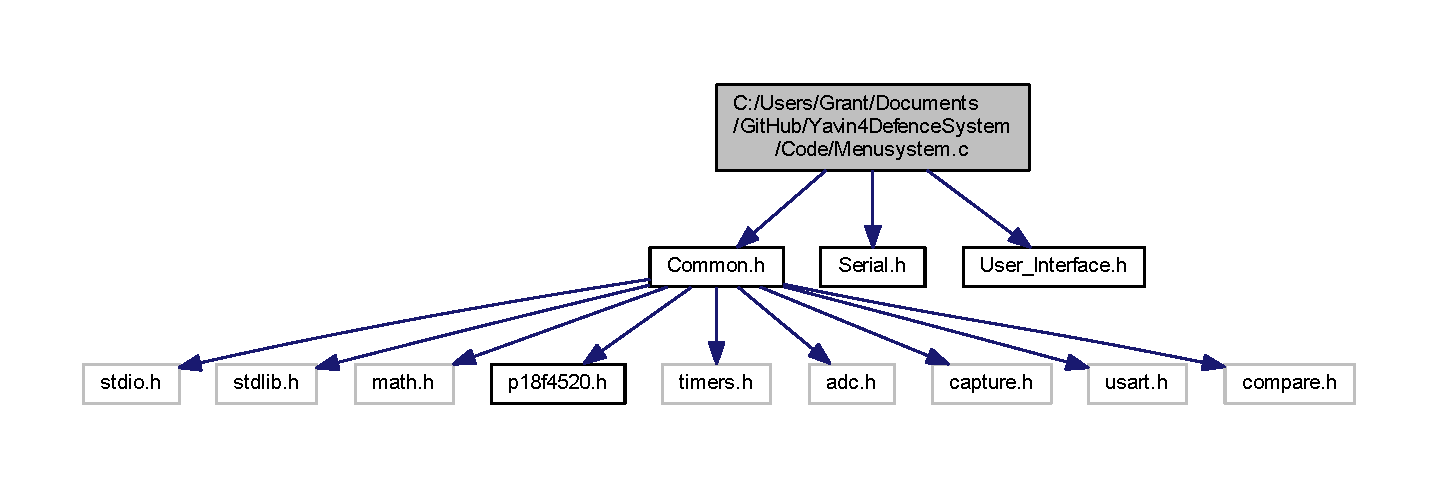
\includegraphics[width=350pt]{_menusystem_8c__incl}
\end{center}
\end{figure}
\subsection*{Macros}
\begin{DoxyCompactItemize}
\item 
\#define \hyperlink{_menusystem_8c_a667b04d7fb6ef46db4da4af554c5b6f7}{width}~80
\item 
\#define \hyperlink{_menusystem_8c_a64f9f90ece96c7bab4aee3deacf170e0}{height}~24
\item 
\#define \hyperlink{_menusystem_8c_a59e24be624462b0016d40f9ada6bbb69}{top1}~0x\+F\+F
\item 
\#define \hyperlink{_menusystem_8c_ac6732d277bcb2f666784f4f3f5e17f39}{auto11}~0x10
\item 
\#define \hyperlink{_menusystem_8c_abed1ba920ec7390cfb509ce3d3b514eb}{manu12}~0x20
\item 
\#define \hyperlink{_menusystem_8c_a65912490d63985a47ca283029e911b2b}{manugoto121}~0x21
\item 
\#define \hyperlink{_menusystem_8c_abae4a42361e301d3ac9dbb5aad94f03d}{manusetl122}~0x22
\item 
\#define \hyperlink{_menusystem_8c_a257270ed391fc5cf1577e20beb72b82d}{manushow123}~0x23
\item 
\#define \hyperlink{_menusystem_8c_ae60b73d9ad027f8210c2a7789349428b}{stat13}~0x30
\item 
\#define \hyperlink{_menusystem_8c_a99fdb7c018e6ad7decf89ca228db518f}{swap14}~0x40
\item 
\#define \hyperlink{_menusystem_8c_a38bd38059a23acf74ca3559d13c2a6d5}{slee15}~0x50
\end{DoxyCompactItemize}
\subsection*{Functions}
\begin{DoxyCompactItemize}
\item 
void \hyperlink{_menusystem_8c_afa234d458057237e03e355d30fafac84}{menu} (char menuselect)
\item 
void \hyperlink{_menusystem_8c_a4ec0accaddbc5d42e2c1cf77d22693c3}{topmenu} (void)
\item 
void \hyperlink{_menusystem_8c_a4437457cad71a9015dbfbac75f9b2b99}{topmenudisp} (void)
\item 
void \hyperlink{_menusystem_8c_ae3777c5b2ceab74d5d90b444da874d14}{disptoptions} (void)
\item 
void \hyperlink{_menusystem_8c_aec49123d1c8f1231607dc9159ae138a4}{clearscreen} (char length)
\item 
void \hyperlink{_menusystem_8c_a4bb64cc936229611900f25e483381dc7}{filler} (char length)
\item 
void \hyperlink{_menusystem_8c_a94b96ccbb8f3c627c5d59189498a3c1b}{initialise\+Menu} (void)
\begin{DoxyCompactList}\small\item\em Initialises the menu system. \end{DoxyCompactList}\item 
void \hyperlink{_menusystem_8c_afc5a5c12a076ae6c7424df4f4124a521}{service\+Menu} (void)
\begin{DoxyCompactList}\small\item\em services any user interface with the menu \end{DoxyCompactList}\item 
void \hyperlink{_menusystem_8c_a0f329206447b1f40e6f730b346aaaf44}{menu\+I\+S\+R} (void)
\begin{DoxyCompactList}\small\item\em I\+S\+R function for the menu subsystem. \end{DoxyCompactList}\end{DoxyCompactItemize}
\subsection*{Variables}
\begin{DoxyCompactItemize}
\item 
char \hyperlink{_menusystem_8c_a5ba864b4bbe4a84e0ca85b979ec2c10b}{t\+M\+E\+S\+S\+A\+G\+E} \mbox{[}$\,$\mbox{]} = \char`\"{}Hello 123\textbackslash{}n\char`\"{}
\item 
char \hyperlink{_menusystem_8c_ae6c5caedc34899ea80a6b011fec5f2a4}{fillerthing} \mbox{[}$\,$\mbox{]} = \char`\"{}+\char`\"{}
\item 
char \hyperlink{_menusystem_8c_a3e47bea989735dbc22688e1ee25ebe9c}{newline} \mbox{[}$\,$\mbox{]} = \char`\"{}\textbackslash{}n\char`\"{}
\item 
char \hyperlink{_menusystem_8c_a9cb97c7ce3babec16a2e500625985994}{choose} \mbox{[}$\,$\mbox{]} = \char`\"{}\textbackslash{}t\+Please select your option (eg. 2)\+: \textbackslash{}n\char`\"{}
\item 
char \hyperlink{_menusystem_8c_a009126ac947a1079b52555366ac7b7f3}{goup} \mbox{[}$\,$\mbox{]} = \char`\"{}\textbackslash{}t\+Up a level\textbackslash{}n\char`\"{}
\item 
char \hyperlink{_menusystem_8c_a532e72c4b620eecff97eee6b0eed5bdd}{welcome} \mbox{[}$\,$\mbox{]} = \char`\"{}Welcome to Yavin I\+V Defence System\char`\"{}
\item 
char \hyperlink{_menusystem_8c_a1985e3f1b27ce97bff59359bed67bd58}{topoption1} \mbox{[}$\,$\mbox{]} = \char`\"{}\textbackslash{}t1\+:\textbackslash{}t\+Automatic Tracking\textbackslash{}n\char`\"{}
\item 
char \hyperlink{_menusystem_8c_acefc91d5187b4570470476a6cd0b68e9}{topoption2} \mbox{[}$\,$\mbox{]} = \char`\"{}\textbackslash{}t2\+:\textbackslash{}t\+Manual Tracking\textbackslash{}n\char`\"{}
\item 
char \hyperlink{_menusystem_8c_ac241270fe5f174769b3034e81c0a574e}{topoption3} \mbox{[}$\,$\mbox{]} = \char`\"{}\textbackslash{}t3\+:\textbackslash{}t\+Status\textbackslash{}n\char`\"{}
\item 
char \hyperlink{_menusystem_8c_a5d44776e05294f14fa1a49e2c9b4820f}{topoption4} \mbox{[}$\,$\mbox{]} = \char`\"{}\textbackslash{}t4\+:\textbackslash{}t\+Go To Local Mode\textbackslash{}n\char`\"{}
\item 
char \hyperlink{_menusystem_8c_a53c72e5e662134afa6e04b4f2aa2863c}{topoption5} \mbox{[}$\,$\mbox{]} = \char`\"{}\textbackslash{}t5\+:\textbackslash{}t\+Sleep\textbackslash{}n\char`\"{}
\end{DoxyCompactItemize}


\subsection{Macro Definition Documentation}
\hypertarget{_menusystem_8c_ac6732d277bcb2f666784f4f3f5e17f39}{\index{Menusystem.\+c@{Menusystem.\+c}!auto11@{auto11}}
\index{auto11@{auto11}!Menusystem.\+c@{Menusystem.\+c}}
\subsubsection[{auto11}]{\setlength{\rightskip}{0pt plus 5cm}\#define auto11~0x10}}\label{_menusystem_8c_ac6732d277bcb2f666784f4f3f5e17f39}


Definition at line 9 of file Menusystem.\+c.

\hypertarget{_menusystem_8c_a64f9f90ece96c7bab4aee3deacf170e0}{\index{Menusystem.\+c@{Menusystem.\+c}!height@{height}}
\index{height@{height}!Menusystem.\+c@{Menusystem.\+c}}
\subsubsection[{height}]{\setlength{\rightskip}{0pt plus 5cm}\#define height~24}}\label{_menusystem_8c_a64f9f90ece96c7bab4aee3deacf170e0}


Definition at line 6 of file Menusystem.\+c.

\hypertarget{_menusystem_8c_abed1ba920ec7390cfb509ce3d3b514eb}{\index{Menusystem.\+c@{Menusystem.\+c}!manu12@{manu12}}
\index{manu12@{manu12}!Menusystem.\+c@{Menusystem.\+c}}
\subsubsection[{manu12}]{\setlength{\rightskip}{0pt plus 5cm}\#define manu12~0x20}}\label{_menusystem_8c_abed1ba920ec7390cfb509ce3d3b514eb}


Definition at line 10 of file Menusystem.\+c.

\hypertarget{_menusystem_8c_a65912490d63985a47ca283029e911b2b}{\index{Menusystem.\+c@{Menusystem.\+c}!manugoto121@{manugoto121}}
\index{manugoto121@{manugoto121}!Menusystem.\+c@{Menusystem.\+c}}
\subsubsection[{manugoto121}]{\setlength{\rightskip}{0pt plus 5cm}\#define manugoto121~0x21}}\label{_menusystem_8c_a65912490d63985a47ca283029e911b2b}


Definition at line 11 of file Menusystem.\+c.

\hypertarget{_menusystem_8c_abae4a42361e301d3ac9dbb5aad94f03d}{\index{Menusystem.\+c@{Menusystem.\+c}!manusetl122@{manusetl122}}
\index{manusetl122@{manusetl122}!Menusystem.\+c@{Menusystem.\+c}}
\subsubsection[{manusetl122}]{\setlength{\rightskip}{0pt plus 5cm}\#define manusetl122~0x22}}\label{_menusystem_8c_abae4a42361e301d3ac9dbb5aad94f03d}


Definition at line 12 of file Menusystem.\+c.

\hypertarget{_menusystem_8c_a257270ed391fc5cf1577e20beb72b82d}{\index{Menusystem.\+c@{Menusystem.\+c}!manushow123@{manushow123}}
\index{manushow123@{manushow123}!Menusystem.\+c@{Menusystem.\+c}}
\subsubsection[{manushow123}]{\setlength{\rightskip}{0pt plus 5cm}\#define manushow123~0x23}}\label{_menusystem_8c_a257270ed391fc5cf1577e20beb72b82d}


Definition at line 13 of file Menusystem.\+c.

\hypertarget{_menusystem_8c_a38bd38059a23acf74ca3559d13c2a6d5}{\index{Menusystem.\+c@{Menusystem.\+c}!slee15@{slee15}}
\index{slee15@{slee15}!Menusystem.\+c@{Menusystem.\+c}}
\subsubsection[{slee15}]{\setlength{\rightskip}{0pt plus 5cm}\#define slee15~0x50}}\label{_menusystem_8c_a38bd38059a23acf74ca3559d13c2a6d5}


Definition at line 17 of file Menusystem.\+c.

\hypertarget{_menusystem_8c_ae60b73d9ad027f8210c2a7789349428b}{\index{Menusystem.\+c@{Menusystem.\+c}!stat13@{stat13}}
\index{stat13@{stat13}!Menusystem.\+c@{Menusystem.\+c}}
\subsubsection[{stat13}]{\setlength{\rightskip}{0pt plus 5cm}\#define stat13~0x30}}\label{_menusystem_8c_ae60b73d9ad027f8210c2a7789349428b}


Definition at line 15 of file Menusystem.\+c.

\hypertarget{_menusystem_8c_a99fdb7c018e6ad7decf89ca228db518f}{\index{Menusystem.\+c@{Menusystem.\+c}!swap14@{swap14}}
\index{swap14@{swap14}!Menusystem.\+c@{Menusystem.\+c}}
\subsubsection[{swap14}]{\setlength{\rightskip}{0pt plus 5cm}\#define swap14~0x40}}\label{_menusystem_8c_a99fdb7c018e6ad7decf89ca228db518f}


Definition at line 16 of file Menusystem.\+c.

\hypertarget{_menusystem_8c_a59e24be624462b0016d40f9ada6bbb69}{\index{Menusystem.\+c@{Menusystem.\+c}!top1@{top1}}
\index{top1@{top1}!Menusystem.\+c@{Menusystem.\+c}}
\subsubsection[{top1}]{\setlength{\rightskip}{0pt plus 5cm}\#define top1~0x\+F\+F}}\label{_menusystem_8c_a59e24be624462b0016d40f9ada6bbb69}


Definition at line 8 of file Menusystem.\+c.

\hypertarget{_menusystem_8c_a667b04d7fb6ef46db4da4af554c5b6f7}{\index{Menusystem.\+c@{Menusystem.\+c}!width@{width}}
\index{width@{width}!Menusystem.\+c@{Menusystem.\+c}}
\subsubsection[{width}]{\setlength{\rightskip}{0pt plus 5cm}\#define width~80}}\label{_menusystem_8c_a667b04d7fb6ef46db4da4af554c5b6f7}


Definition at line 5 of file Menusystem.\+c.



\subsection{Function Documentation}
\hypertarget{_menusystem_8c_aec49123d1c8f1231607dc9159ae138a4}{\index{Menusystem.\+c@{Menusystem.\+c}!clearscreen@{clearscreen}}
\index{clearscreen@{clearscreen}!Menusystem.\+c@{Menusystem.\+c}}
\subsubsection[{clearscreen}]{\setlength{\rightskip}{0pt plus 5cm}void clearscreen (
\begin{DoxyParamCaption}
\item[{char}]{length}
\end{DoxyParamCaption}
)}}\label{_menusystem_8c_aec49123d1c8f1231607dc9159ae138a4}


Definition at line 43 of file Menusystem.\+c.



Here is the call graph for this function\+:
\nopagebreak
\begin{figure}[H]
\begin{center}
\leavevmode
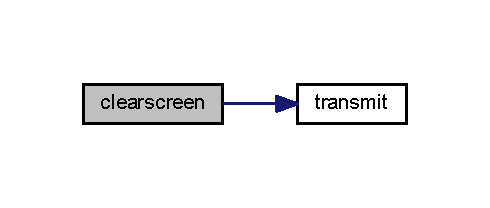
\includegraphics[width=235pt]{_menusystem_8c_aec49123d1c8f1231607dc9159ae138a4_cgraph}
\end{center}
\end{figure}




Here is the caller graph for this function\+:
\nopagebreak
\begin{figure}[H]
\begin{center}
\leavevmode
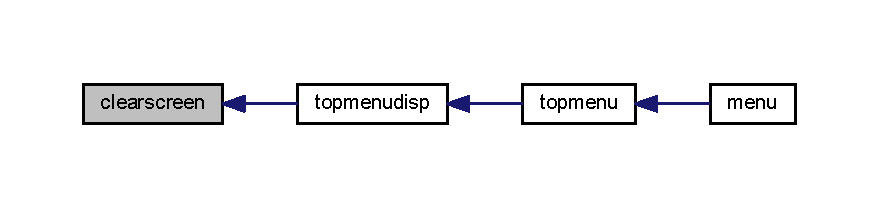
\includegraphics[width=350pt]{_menusystem_8c_aec49123d1c8f1231607dc9159ae138a4_icgraph}
\end{center}
\end{figure}


\hypertarget{_menusystem_8c_ae3777c5b2ceab74d5d90b444da874d14}{\index{Menusystem.\+c@{Menusystem.\+c}!disptoptions@{disptoptions}}
\index{disptoptions@{disptoptions}!Menusystem.\+c@{Menusystem.\+c}}
\subsubsection[{disptoptions}]{\setlength{\rightskip}{0pt plus 5cm}void disptoptions (
\begin{DoxyParamCaption}
\item[{void}]{}
\end{DoxyParamCaption}
)}}\label{_menusystem_8c_ae3777c5b2ceab74d5d90b444da874d14}


Definition at line 57 of file Menusystem.\+c.



Here is the call graph for this function\+:
\nopagebreak
\begin{figure}[H]
\begin{center}
\leavevmode
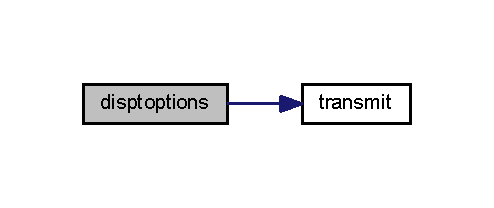
\includegraphics[width=237pt]{_menusystem_8c_ae3777c5b2ceab74d5d90b444da874d14_cgraph}
\end{center}
\end{figure}




Here is the caller graph for this function\+:
\nopagebreak
\begin{figure}[H]
\begin{center}
\leavevmode
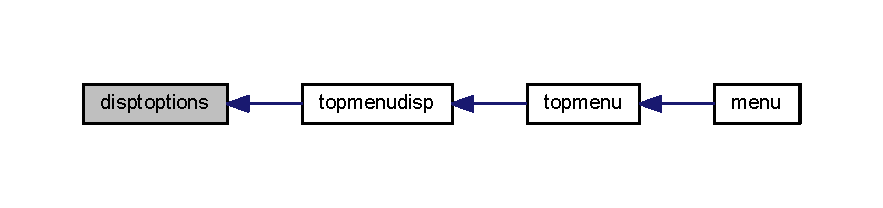
\includegraphics[width=350pt]{_menusystem_8c_ae3777c5b2ceab74d5d90b444da874d14_icgraph}
\end{center}
\end{figure}


\hypertarget{_menusystem_8c_a4bb64cc936229611900f25e483381dc7}{\index{Menusystem.\+c@{Menusystem.\+c}!filler@{filler}}
\index{filler@{filler}!Menusystem.\+c@{Menusystem.\+c}}
\subsubsection[{filler}]{\setlength{\rightskip}{0pt plus 5cm}void filler (
\begin{DoxyParamCaption}
\item[{char}]{length}
\end{DoxyParamCaption}
)}}\label{_menusystem_8c_a4bb64cc936229611900f25e483381dc7}


Definition at line 50 of file Menusystem.\+c.



Here is the call graph for this function\+:
\nopagebreak
\begin{figure}[H]
\begin{center}
\leavevmode
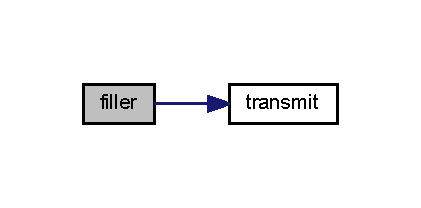
\includegraphics[width=202pt]{_menusystem_8c_a4bb64cc936229611900f25e483381dc7_cgraph}
\end{center}
\end{figure}




Here is the caller graph for this function\+:
\nopagebreak
\begin{figure}[H]
\begin{center}
\leavevmode
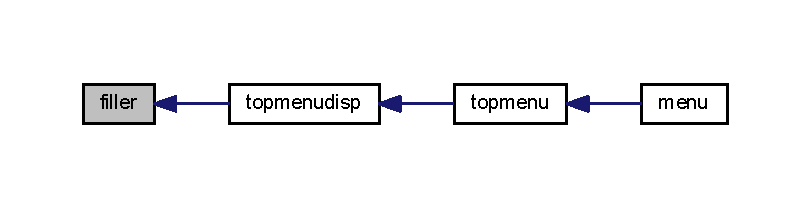
\includegraphics[width=350pt]{_menusystem_8c_a4bb64cc936229611900f25e483381dc7_icgraph}
\end{center}
\end{figure}


\hypertarget{_menusystem_8c_a94b96ccbb8f3c627c5d59189498a3c1b}{\index{Menusystem.\+c@{Menusystem.\+c}!initialise\+Menu@{initialise\+Menu}}
\index{initialise\+Menu@{initialise\+Menu}!Menusystem.\+c@{Menusystem.\+c}}
\subsubsection[{initialise\+Menu}]{\setlength{\rightskip}{0pt plus 5cm}void initialise\+Menu (
\begin{DoxyParamCaption}
\item[{void}]{}
\end{DoxyParamCaption}
)}}\label{_menusystem_8c_a94b96ccbb8f3c627c5d59189498a3c1b}


Initialises the menu system. 



 Function\+: \hyperlink{_menusystem_8c_a94b96ccbb8f3c627c5d59189498a3c1b}{initialise\+Menu(void)}

Include\+: \hyperlink{_menusystem_8h}{Menusystem.\+h}

Description\+: initialises the menu system so that it is fully operational

Arguments\+: None

Returns\+: None 

Definition at line 135 of file Menusystem.\+c.

\hypertarget{_menusystem_8c_afa234d458057237e03e355d30fafac84}{\index{Menusystem.\+c@{Menusystem.\+c}!menu@{menu}}
\index{menu@{menu}!Menusystem.\+c@{Menusystem.\+c}}
\subsubsection[{menu}]{\setlength{\rightskip}{0pt plus 5cm}void menu (
\begin{DoxyParamCaption}
\item[{char}]{menuselect}
\end{DoxyParamCaption}
)}}\label{_menusystem_8c_afa234d458057237e03e355d30fafac84}
Call the serial configuration to enable U\+S\+A\+R\+T Subsysten 

Definition at line 182 of file Menusystem.\+c.



Here is the call graph for this function\+:
\nopagebreak
\begin{figure}[H]
\begin{center}
\leavevmode
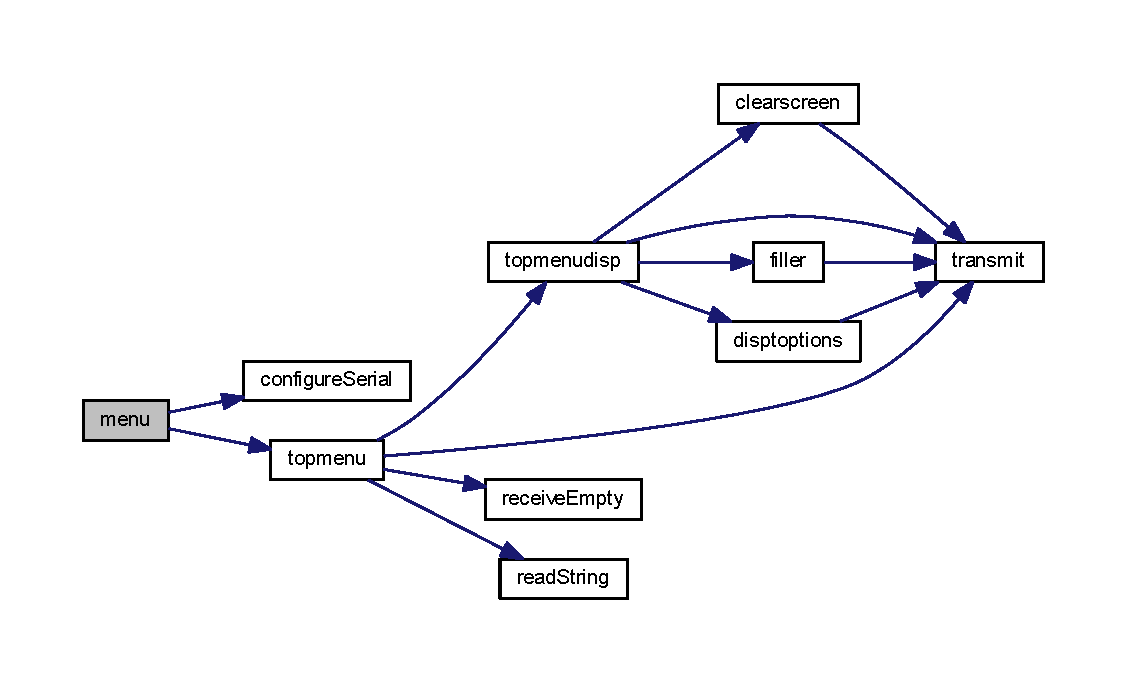
\includegraphics[width=350pt]{_menusystem_8c_afa234d458057237e03e355d30fafac84_cgraph}
\end{center}
\end{figure}


\hypertarget{_menusystem_8c_a0f329206447b1f40e6f730b346aaaf44}{\index{Menusystem.\+c@{Menusystem.\+c}!menu\+I\+S\+R@{menu\+I\+S\+R}}
\index{menu\+I\+S\+R@{menu\+I\+S\+R}!Menusystem.\+c@{Menusystem.\+c}}
\subsubsection[{menu\+I\+S\+R}]{\setlength{\rightskip}{0pt plus 5cm}void menu\+I\+S\+R (
\begin{DoxyParamCaption}
\item[{void}]{}
\end{DoxyParamCaption}
)}}\label{_menusystem_8c_a0f329206447b1f40e6f730b346aaaf44}


I\+S\+R function for the menu subsystem. 



 Function\+: \hyperlink{_menusystem_8c_a0f329206447b1f40e6f730b346aaaf44}{menu\+I\+S\+R(void)}

Include\+: \hyperlink{_menusystem_8h}{Menusystem.\+h}

Description\+: services any interrupts associated with the menu system

Arguments\+: None

Returns\+: None 

Definition at line 177 of file Menusystem.\+c.

\hypertarget{_menusystem_8c_afc5a5c12a076ae6c7424df4f4124a521}{\index{Menusystem.\+c@{Menusystem.\+c}!service\+Menu@{service\+Menu}}
\index{service\+Menu@{service\+Menu}!Menusystem.\+c@{Menusystem.\+c}}
\subsubsection[{service\+Menu}]{\setlength{\rightskip}{0pt plus 5cm}void service\+Menu (
\begin{DoxyParamCaption}
\item[{void}]{}
\end{DoxyParamCaption}
)}}\label{_menusystem_8c_afc5a5c12a076ae6c7424df4f4124a521}


services any user interface with the menu 



 Function\+: \hyperlink{_menusystem_8c_afc5a5c12a076ae6c7424df4f4124a521}{service\+Menu(void)}

Include\+:

Description\+: Checks if the user has made any inputs to the system. If not the function simply returns. If they have then it services the inputs, displays the correct outputs and performs the specified actions

Arguments\+: None

Returns\+: None 

Definition at line 158 of file Menusystem.\+c.

\hypertarget{_menusystem_8c_a4ec0accaddbc5d42e2c1cf77d22693c3}{\index{Menusystem.\+c@{Menusystem.\+c}!topmenu@{topmenu}}
\index{topmenu@{topmenu}!Menusystem.\+c@{Menusystem.\+c}}
\subsubsection[{topmenu}]{\setlength{\rightskip}{0pt plus 5cm}void topmenu (
\begin{DoxyParamCaption}
\item[{void}]{}
\end{DoxyParamCaption}
)}}\label{_menusystem_8c_a4ec0accaddbc5d42e2c1cf77d22693c3}
Display the menu screen via serial wait for/get serial input make decision based on input

Wait until the receive buffer is no longer empty

Indicating that a command has been passed

Reset status flag

Get the input string and store it in 

test 

Definition at line 83 of file Menusystem.\+c.



Here is the call graph for this function\+:
\nopagebreak
\begin{figure}[H]
\begin{center}
\leavevmode
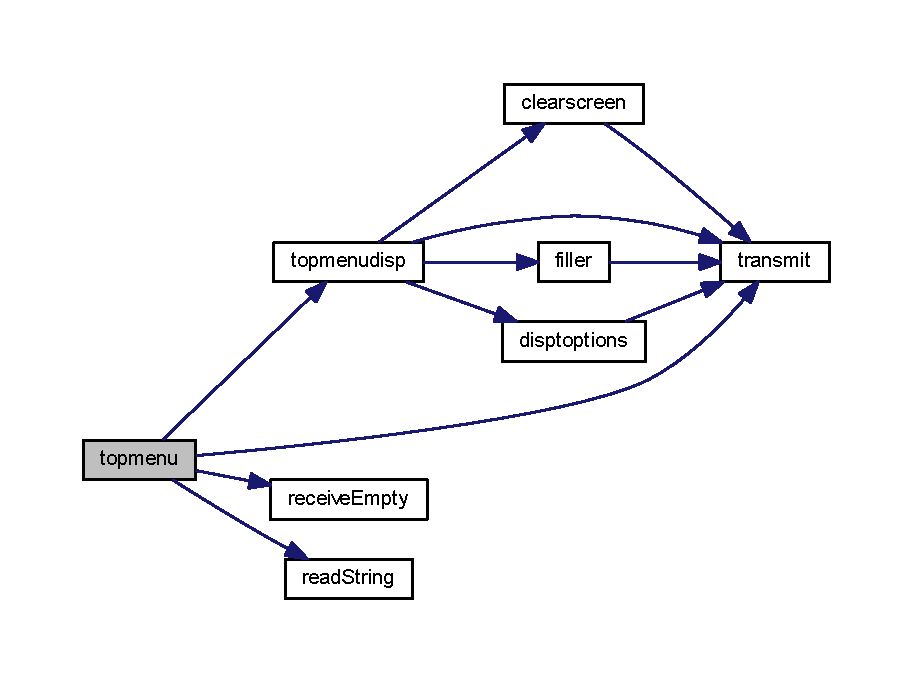
\includegraphics[width=350pt]{_menusystem_8c_a4ec0accaddbc5d42e2c1cf77d22693c3_cgraph}
\end{center}
\end{figure}




Here is the caller graph for this function\+:
\nopagebreak
\begin{figure}[H]
\begin{center}
\leavevmode
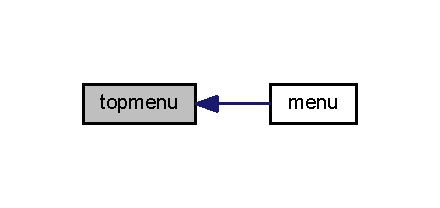
\includegraphics[width=211pt]{_menusystem_8c_a4ec0accaddbc5d42e2c1cf77d22693c3_icgraph}
\end{center}
\end{figure}


\hypertarget{_menusystem_8c_a4437457cad71a9015dbfbac75f9b2b99}{\index{Menusystem.\+c@{Menusystem.\+c}!topmenudisp@{topmenudisp}}
\index{topmenudisp@{topmenudisp}!Menusystem.\+c@{Menusystem.\+c}}
\subsubsection[{topmenudisp}]{\setlength{\rightskip}{0pt plus 5cm}void topmenudisp (
\begin{DoxyParamCaption}
\item[{void}]{}
\end{DoxyParamCaption}
)}}\label{_menusystem_8c_a4437457cad71a9015dbfbac75f9b2b99}


Definition at line 65 of file Menusystem.\+c.



Here is the call graph for this function\+:
\nopagebreak
\begin{figure}[H]
\begin{center}
\leavevmode
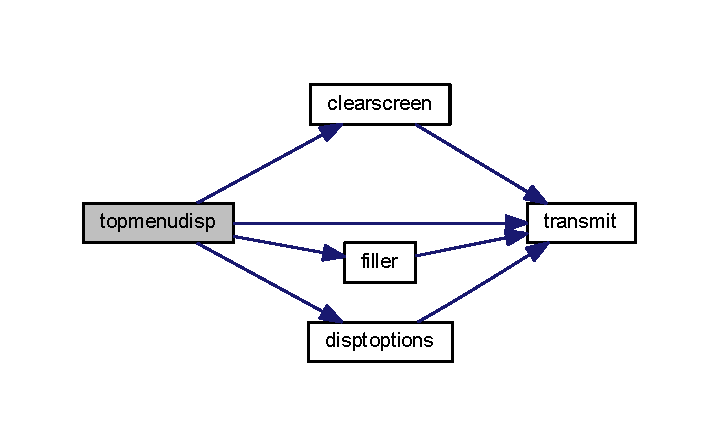
\includegraphics[width=345pt]{_menusystem_8c_a4437457cad71a9015dbfbac75f9b2b99_cgraph}
\end{center}
\end{figure}




Here is the caller graph for this function\+:
\nopagebreak
\begin{figure}[H]
\begin{center}
\leavevmode
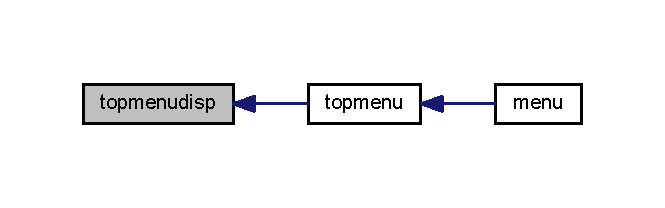
\includegraphics[width=319pt]{_menusystem_8c_a4437457cad71a9015dbfbac75f9b2b99_icgraph}
\end{center}
\end{figure}




\subsection{Variable Documentation}
\hypertarget{_menusystem_8c_a9cb97c7ce3babec16a2e500625985994}{\index{Menusystem.\+c@{Menusystem.\+c}!choose@{choose}}
\index{choose@{choose}!Menusystem.\+c@{Menusystem.\+c}}
\subsubsection[{choose}]{\setlength{\rightskip}{0pt plus 5cm}char choose\mbox{[}$\,$\mbox{]} = \char`\"{}\textbackslash{}t\+Please select your option (eg. 2)\+: \textbackslash{}n\char`\"{}}}\label{_menusystem_8c_a9cb97c7ce3babec16a2e500625985994}


Definition at line 23 of file Menusystem.\+c.

\hypertarget{_menusystem_8c_ae6c5caedc34899ea80a6b011fec5f2a4}{\index{Menusystem.\+c@{Menusystem.\+c}!fillerthing@{fillerthing}}
\index{fillerthing@{fillerthing}!Menusystem.\+c@{Menusystem.\+c}}
\subsubsection[{fillerthing}]{\setlength{\rightskip}{0pt plus 5cm}char fillerthing\mbox{[}$\,$\mbox{]} = \char`\"{}+\char`\"{}}}\label{_menusystem_8c_ae6c5caedc34899ea80a6b011fec5f2a4}


Definition at line 21 of file Menusystem.\+c.

\hypertarget{_menusystem_8c_a009126ac947a1079b52555366ac7b7f3}{\index{Menusystem.\+c@{Menusystem.\+c}!goup@{goup}}
\index{goup@{goup}!Menusystem.\+c@{Menusystem.\+c}}
\subsubsection[{goup}]{\setlength{\rightskip}{0pt plus 5cm}char goup\mbox{[}$\,$\mbox{]} = \char`\"{}\textbackslash{}t\+Up a level\textbackslash{}n\char`\"{}}}\label{_menusystem_8c_a009126ac947a1079b52555366ac7b7f3}


Definition at line 24 of file Menusystem.\+c.

\hypertarget{_menusystem_8c_a3e47bea989735dbc22688e1ee25ebe9c}{\index{Menusystem.\+c@{Menusystem.\+c}!newline@{newline}}
\index{newline@{newline}!Menusystem.\+c@{Menusystem.\+c}}
\subsubsection[{newline}]{\setlength{\rightskip}{0pt plus 5cm}char newline\mbox{[}$\,$\mbox{]} = \char`\"{}\textbackslash{}n\char`\"{}}}\label{_menusystem_8c_a3e47bea989735dbc22688e1ee25ebe9c}


Definition at line 22 of file Menusystem.\+c.

\hypertarget{_menusystem_8c_a5ba864b4bbe4a84e0ca85b979ec2c10b}{\index{Menusystem.\+c@{Menusystem.\+c}!t\+M\+E\+S\+S\+A\+G\+E@{t\+M\+E\+S\+S\+A\+G\+E}}
\index{t\+M\+E\+S\+S\+A\+G\+E@{t\+M\+E\+S\+S\+A\+G\+E}!Menusystem.\+c@{Menusystem.\+c}}
\subsubsection[{t\+M\+E\+S\+S\+A\+G\+E}]{\setlength{\rightskip}{0pt plus 5cm}char t\+M\+E\+S\+S\+A\+G\+E\mbox{[}$\,$\mbox{]} = \char`\"{}Hello 123\textbackslash{}n\char`\"{}}}\label{_menusystem_8c_a5ba864b4bbe4a84e0ca85b979ec2c10b}


Definition at line 20 of file Menusystem.\+c.

\hypertarget{_menusystem_8c_a1985e3f1b27ce97bff59359bed67bd58}{\index{Menusystem.\+c@{Menusystem.\+c}!topoption1@{topoption1}}
\index{topoption1@{topoption1}!Menusystem.\+c@{Menusystem.\+c}}
\subsubsection[{topoption1}]{\setlength{\rightskip}{0pt plus 5cm}char topoption1\mbox{[}$\,$\mbox{]} = \char`\"{}\textbackslash{}t1\+:\textbackslash{}t\+Automatic Tracking\textbackslash{}n\char`\"{}}}\label{_menusystem_8c_a1985e3f1b27ce97bff59359bed67bd58}


Definition at line 29 of file Menusystem.\+c.

\hypertarget{_menusystem_8c_acefc91d5187b4570470476a6cd0b68e9}{\index{Menusystem.\+c@{Menusystem.\+c}!topoption2@{topoption2}}
\index{topoption2@{topoption2}!Menusystem.\+c@{Menusystem.\+c}}
\subsubsection[{topoption2}]{\setlength{\rightskip}{0pt plus 5cm}char topoption2\mbox{[}$\,$\mbox{]} = \char`\"{}\textbackslash{}t2\+:\textbackslash{}t\+Manual Tracking\textbackslash{}n\char`\"{}}}\label{_menusystem_8c_acefc91d5187b4570470476a6cd0b68e9}


Definition at line 30 of file Menusystem.\+c.

\hypertarget{_menusystem_8c_ac241270fe5f174769b3034e81c0a574e}{\index{Menusystem.\+c@{Menusystem.\+c}!topoption3@{topoption3}}
\index{topoption3@{topoption3}!Menusystem.\+c@{Menusystem.\+c}}
\subsubsection[{topoption3}]{\setlength{\rightskip}{0pt plus 5cm}char topoption3\mbox{[}$\,$\mbox{]} = \char`\"{}\textbackslash{}t3\+:\textbackslash{}t\+Status\textbackslash{}n\char`\"{}}}\label{_menusystem_8c_ac241270fe5f174769b3034e81c0a574e}


Definition at line 31 of file Menusystem.\+c.

\hypertarget{_menusystem_8c_a5d44776e05294f14fa1a49e2c9b4820f}{\index{Menusystem.\+c@{Menusystem.\+c}!topoption4@{topoption4}}
\index{topoption4@{topoption4}!Menusystem.\+c@{Menusystem.\+c}}
\subsubsection[{topoption4}]{\setlength{\rightskip}{0pt plus 5cm}char topoption4\mbox{[}$\,$\mbox{]} = \char`\"{}\textbackslash{}t4\+:\textbackslash{}t\+Go To Local Mode\textbackslash{}n\char`\"{}}}\label{_menusystem_8c_a5d44776e05294f14fa1a49e2c9b4820f}


Definition at line 32 of file Menusystem.\+c.

\hypertarget{_menusystem_8c_a53c72e5e662134afa6e04b4f2aa2863c}{\index{Menusystem.\+c@{Menusystem.\+c}!topoption5@{topoption5}}
\index{topoption5@{topoption5}!Menusystem.\+c@{Menusystem.\+c}}
\subsubsection[{topoption5}]{\setlength{\rightskip}{0pt plus 5cm}char topoption5\mbox{[}$\,$\mbox{]} = \char`\"{}\textbackslash{}t5\+:\textbackslash{}t\+Sleep\textbackslash{}n\char`\"{}}}\label{_menusystem_8c_a53c72e5e662134afa6e04b4f2aa2863c}


Definition at line 33 of file Menusystem.\+c.

\hypertarget{_menusystem_8c_a532e72c4b620eecff97eee6b0eed5bdd}{\index{Menusystem.\+c@{Menusystem.\+c}!welcome@{welcome}}
\index{welcome@{welcome}!Menusystem.\+c@{Menusystem.\+c}}
\subsubsection[{welcome}]{\setlength{\rightskip}{0pt plus 5cm}char welcome\mbox{[}$\,$\mbox{]} = \char`\"{}Welcome to Yavin I\+V Defence System\char`\"{}}}\label{_menusystem_8c_a532e72c4b620eecff97eee6b0eed5bdd}


Definition at line 28 of file Menusystem.\+c.


\hypertarget{_menusystem_8h}{\section{Menusystem.\+h File Reference}
\label{_menusystem_8h}\index{Menusystem.\+h@{Menusystem.\+h}}
}
This graph shows which files directly or indirectly include this file\+:\nopagebreak
\begin{figure}[H]
\begin{center}
\leavevmode
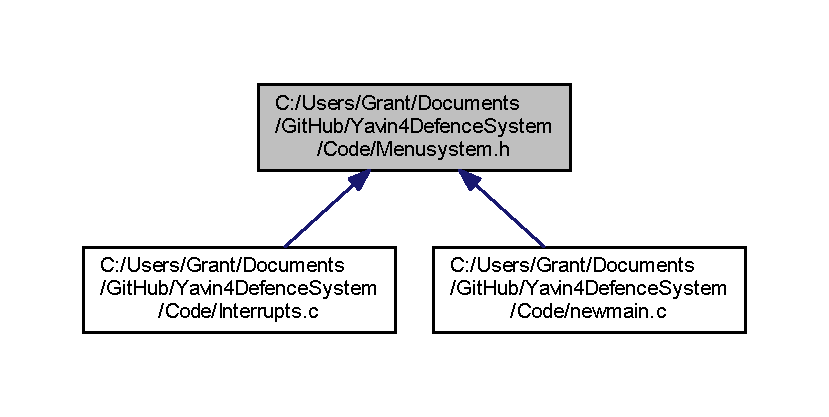
\includegraphics[width=226pt]{_menusystem_8h__dep__incl}
\end{center}
\end{figure}
\subsection*{Macros}
\begin{DoxyCompactItemize}
\item 
\#define \hyperlink{_menusystem_8h_abe3db97a849df459252001e1f4b3721c}{M\+E\+N\+U\+\_\+\+I\+S\+R}~0
\item 
\#define \hyperlink{_menusystem_8h_a9552ba249c0540ffe9a08a05d1b92504}{M\+E\+N\+U\+\_\+\+H}
\end{DoxyCompactItemize}
\subsection*{Functions}
\begin{DoxyCompactItemize}
\item 
void \hyperlink{_menusystem_8h_a94b96ccbb8f3c627c5d59189498a3c1b}{initialise\+Menu} (void)
\begin{DoxyCompactList}\small\item\em Initialises the menu system. \end{DoxyCompactList}\item 
void \hyperlink{_menusystem_8h_afc5a5c12a076ae6c7424df4f4124a521}{service\+Menu} (void)
\begin{DoxyCompactList}\small\item\em services any user interface with the menu \end{DoxyCompactList}\item 
void \hyperlink{_menusystem_8h_a0f329206447b1f40e6f730b346aaaf44}{menu\+I\+S\+R} (void)
\begin{DoxyCompactList}\small\item\em I\+S\+R function for the menu subsystem. \end{DoxyCompactList}\item 
void \hyperlink{_menusystem_8h_ad16e5e62f3579a7048e6b981b172885e}{menu} (void)
\end{DoxyCompactItemize}


\subsection{Macro Definition Documentation}
\hypertarget{_menusystem_8h_a9552ba249c0540ffe9a08a05d1b92504}{\index{Menusystem.\+h@{Menusystem.\+h}!M\+E\+N\+U\+\_\+\+H@{M\+E\+N\+U\+\_\+\+H}}
\index{M\+E\+N\+U\+\_\+\+H@{M\+E\+N\+U\+\_\+\+H}!Menusystem.\+h@{Menusystem.\+h}}
\subsubsection[{M\+E\+N\+U\+\_\+\+H}]{\setlength{\rightskip}{0pt plus 5cm}\#define M\+E\+N\+U\+\_\+\+H}}\label{_menusystem_8h_a9552ba249c0540ffe9a08a05d1b92504}


Definition at line 19 of file Menusystem.\+h.

\hypertarget{_menusystem_8h_abe3db97a849df459252001e1f4b3721c}{\index{Menusystem.\+h@{Menusystem.\+h}!M\+E\+N\+U\+\_\+\+I\+S\+R@{M\+E\+N\+U\+\_\+\+I\+S\+R}}
\index{M\+E\+N\+U\+\_\+\+I\+S\+R@{M\+E\+N\+U\+\_\+\+I\+S\+R}!Menusystem.\+h@{Menusystem.\+h}}
\subsubsection[{M\+E\+N\+U\+\_\+\+I\+S\+R}]{\setlength{\rightskip}{0pt plus 5cm}\#define M\+E\+N\+U\+\_\+\+I\+S\+R~0}}\label{_menusystem_8h_abe3db97a849df459252001e1f4b3721c}


Definition at line 11 of file Menusystem.\+h.



\subsection{Function Documentation}
\hypertarget{_menusystem_8h_a94b96ccbb8f3c627c5d59189498a3c1b}{\index{Menusystem.\+h@{Menusystem.\+h}!initialise\+Menu@{initialise\+Menu}}
\index{initialise\+Menu@{initialise\+Menu}!Menusystem.\+h@{Menusystem.\+h}}
\subsubsection[{initialise\+Menu}]{\setlength{\rightskip}{0pt plus 5cm}void initialise\+Menu (
\begin{DoxyParamCaption}
\item[{void}]{}
\end{DoxyParamCaption}
)}}\label{_menusystem_8h_a94b96ccbb8f3c627c5d59189498a3c1b}


Initialises the menu system. 



 Function\+: \hyperlink{_menusystem_8c_a94b96ccbb8f3c627c5d59189498a3c1b}{initialise\+Menu(void)}

Include\+: \hyperlink{_menusystem_8h}{Menusystem.\+h}

Description\+: initialises the menu system so that it is fully operational

Arguments\+: None

Returns\+: None 

Definition at line 148 of file Menusystem.\+c.



Here is the call graph for this function\+:\nopagebreak
\begin{figure}[H]
\begin{center}
\leavevmode
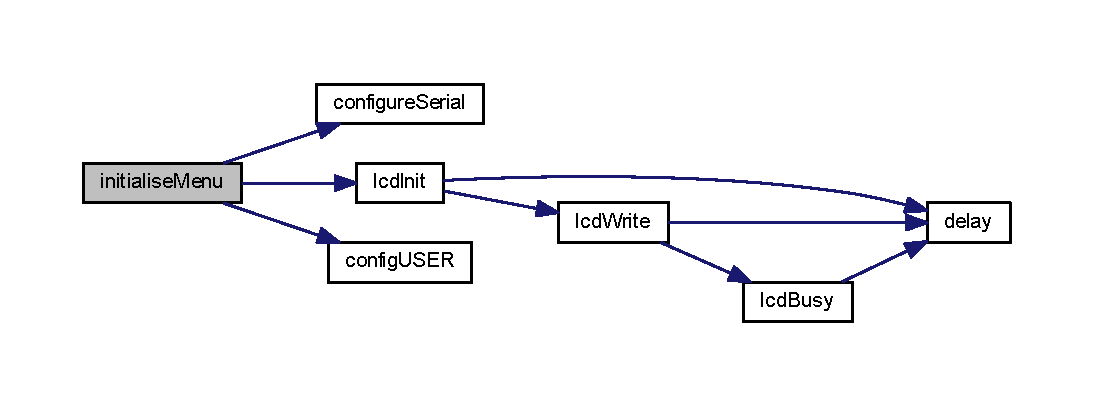
\includegraphics[width=272pt]{_menusystem_8h_a94b96ccbb8f3c627c5d59189498a3c1b_cgraph}
\end{center}
\end{figure}


\hypertarget{_menusystem_8h_ad16e5e62f3579a7048e6b981b172885e}{\index{Menusystem.\+h@{Menusystem.\+h}!menu@{menu}}
\index{menu@{menu}!Menusystem.\+h@{Menusystem.\+h}}
\subsubsection[{menu}]{\setlength{\rightskip}{0pt plus 5cm}void menu (
\begin{DoxyParamCaption}
\item[{void}]{}
\end{DoxyParamCaption}
)}}\label{_menusystem_8h_ad16e5e62f3579a7048e6b981b172885e}
\hypertarget{_menusystem_8h_a0f329206447b1f40e6f730b346aaaf44}{\index{Menusystem.\+h@{Menusystem.\+h}!menu\+I\+S\+R@{menu\+I\+S\+R}}
\index{menu\+I\+S\+R@{menu\+I\+S\+R}!Menusystem.\+h@{Menusystem.\+h}}
\subsubsection[{menu\+I\+S\+R}]{\setlength{\rightskip}{0pt plus 5cm}void menu\+I\+S\+R (
\begin{DoxyParamCaption}
\item[{void}]{}
\end{DoxyParamCaption}
)}}\label{_menusystem_8h_a0f329206447b1f40e6f730b346aaaf44}


I\+S\+R function for the menu subsystem. 



 Function\+: \hyperlink{_menusystem_8c_a0f329206447b1f40e6f730b346aaaf44}{menu\+I\+S\+R(void)}

Include\+: \hyperlink{_menusystem_8h}{Menusystem.\+h}

Description\+: services any interrupts associated with the menu system

Arguments\+: None

Returns\+: None 

Definition at line 190 of file Menusystem.\+c.

\hypertarget{_menusystem_8h_afc5a5c12a076ae6c7424df4f4124a521}{\index{Menusystem.\+h@{Menusystem.\+h}!service\+Menu@{service\+Menu}}
\index{service\+Menu@{service\+Menu}!Menusystem.\+h@{Menusystem.\+h}}
\subsubsection[{service\+Menu}]{\setlength{\rightskip}{0pt plus 5cm}void service\+Menu (
\begin{DoxyParamCaption}
\item[{void}]{}
\end{DoxyParamCaption}
)}}\label{_menusystem_8h_afc5a5c12a076ae6c7424df4f4124a521}


services any user interface with the menu 



 Function\+: \hyperlink{_menusystem_8c_afc5a5c12a076ae6c7424df4f4124a521}{service\+Menu(void)}

Include\+:

Description\+: Checks if the user has made any inputs to the system. If not the function simply returns. If they have then it services the inputs, displays the correct outputs and performs the specified actions

Arguments\+: None

Returns\+: None 

Definition at line 171 of file Menusystem.\+c.



Here is the call graph for this function\+:\nopagebreak
\begin{figure}[H]
\begin{center}
\leavevmode
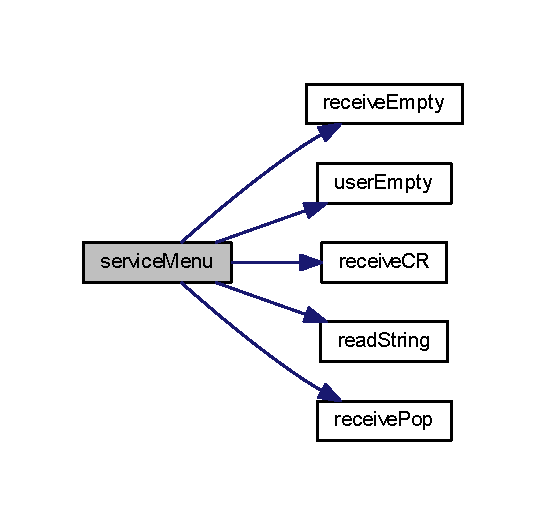
\includegraphics[width=262pt]{_menusystem_8h_afc5a5c12a076ae6c7424df4f4124a521_cgraph}
\end{center}
\end{figure}



\hypertarget{_menusystem2_8c}{\section{C\+:/\+Users/\+Grant/\+Documents/\+Git\+Hub/\+Yavin4\+Defence\+System/\+Code/\+Menusystem2.c File Reference}
\label{_menusystem2_8c}\index{C\+:/\+Users/\+Grant/\+Documents/\+Git\+Hub/\+Yavin4\+Defence\+System/\+Code/\+Menusystem2.\+c@{C\+:/\+Users/\+Grant/\+Documents/\+Git\+Hub/\+Yavin4\+Defence\+System/\+Code/\+Menusystem2.\+c}}
}
{\ttfamily \#include \char`\"{}Common.\+h\char`\"{}}\\*
{\ttfamily \#include \char`\"{}Serial.\+h\char`\"{}}\\*
{\ttfamily \#include \char`\"{}User\+\_\+\+Interface.\+h\char`\"{}}\\*
{\ttfamily \#include \char`\"{}L\+C\+D.\+h\char`\"{}}\\*
{\ttfamily \#include \char`\"{}Pan\+Tilt.\+h\char`\"{}}\\*
Include dependency graph for Menusystem2.\+c\+:
\nopagebreak
\begin{figure}[H]
\begin{center}
\leavevmode
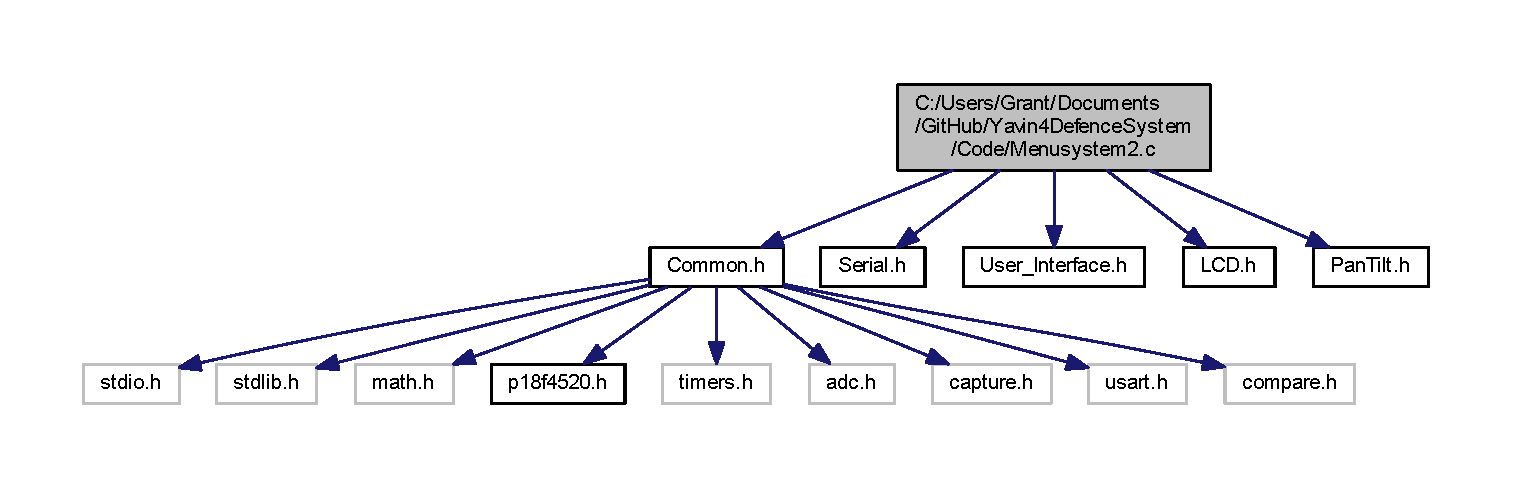
\includegraphics[width=350pt]{_menusystem2_8c__incl}
\end{center}
\end{figure}
\subsection*{Data Structures}
\begin{DoxyCompactItemize}
\item 
struct \hyperlink{struct_sub_menu}{Sub\+Menu}
\end{DoxyCompactItemize}
\subsection*{Macros}
\begin{DoxyCompactItemize}
\item 
\#define \hyperlink{_menusystem2_8c_af3a7cb33a5ae7392934b3197ac67e080}{M\+A\+X\+\_\+\+S\+E\+R\+\_\+\+M\+S\+G\+\_\+\+L\+E\+N}~30
\item 
\#define \hyperlink{_menusystem2_8c_a803e4f9d2e28d9ab24055cb970ea12c3}{M\+A\+X\+\_\+\+L\+C\+D\+\_\+\+M\+S\+G\+\_\+\+L\+E\+N}~20
\item 
\#define \hyperlink{_menusystem2_8c_ab86e62ee54aa604cfbdc4d3048c2845d}{M\+A\+X\+\_\+\+N\+U\+M\+\_\+\+O\+P\+T\+I\+O\+N\+S}~5
\end{DoxyCompactItemize}
\subsection*{Typedefs}
\begin{DoxyCompactItemize}
\item 
typedef struct \hyperlink{struct_sub_menu}{Sub\+Menu} \hyperlink{_menusystem2_8c_a590a7b46cd32899024f14446ecf74f0d}{Sub\+Menu}
\end{DoxyCompactItemize}
\subsection*{Enumerations}
\begin{DoxyCompactItemize}
\item 
enum \hyperlink{_menusystem2_8c_a5c285b48be2dc719a45ce720dcb26870}{Menu\+Level} \{ \hyperlink{_menusystem2_8c_a5c285b48be2dc719a45ce720dcb26870ad41208b99e347d1726824779b11ea11b}{R\+O\+O\+T}, 
\hyperlink{_menusystem2_8c_a5c285b48be2dc719a45ce720dcb26870a12b733d4941495e86811fe6ceeeff9da}{S\+U\+B}, 
\hyperlink{_menusystem2_8c_a5c285b48be2dc719a45ce720dcb26870a389e03ce61ac2d93fd54069187ab58af}{F\+U\+N\+C}
 \}
\end{DoxyCompactItemize}
\subsection*{Functions}
\begin{DoxyCompactItemize}
\item 
void \hyperlink{_menusystem2_8c_a94b96ccbb8f3c627c5d59189498a3c1b}{initialise\+Menu} (void)
\begin{DoxyCompactList}\small\item\em Initialises the menu system. \end{DoxyCompactList}\item 
void \hyperlink{_menusystem2_8c_afc5a5c12a076ae6c7424df4f4124a521}{service\+Menu} (void)
\begin{DoxyCompactList}\small\item\em services any user interface with the menu \end{DoxyCompactList}\item 
void \hyperlink{_menusystem2_8c_a0f329206447b1f40e6f730b346aaaf44}{menu\+I\+S\+R} (void)
\begin{DoxyCompactList}\small\item\em I\+S\+R function for the menu subsystem. \end{DoxyCompactList}\end{DoxyCompactItemize}


\subsection{Macro Definition Documentation}
\hypertarget{_menusystem2_8c_a803e4f9d2e28d9ab24055cb970ea12c3}{\index{Menusystem2.\+c@{Menusystem2.\+c}!M\+A\+X\+\_\+\+L\+C\+D\+\_\+\+M\+S\+G\+\_\+\+L\+E\+N@{M\+A\+X\+\_\+\+L\+C\+D\+\_\+\+M\+S\+G\+\_\+\+L\+E\+N}}
\index{M\+A\+X\+\_\+\+L\+C\+D\+\_\+\+M\+S\+G\+\_\+\+L\+E\+N@{M\+A\+X\+\_\+\+L\+C\+D\+\_\+\+M\+S\+G\+\_\+\+L\+E\+N}!Menusystem2.\+c@{Menusystem2.\+c}}
\subsubsection[{M\+A\+X\+\_\+\+L\+C\+D\+\_\+\+M\+S\+G\+\_\+\+L\+E\+N}]{\setlength{\rightskip}{0pt plus 5cm}\#define M\+A\+X\+\_\+\+L\+C\+D\+\_\+\+M\+S\+G\+\_\+\+L\+E\+N~20}}\label{_menusystem2_8c_a803e4f9d2e28d9ab24055cb970ea12c3}


Definition at line 8 of file Menusystem2.\+c.

\hypertarget{_menusystem2_8c_ab86e62ee54aa604cfbdc4d3048c2845d}{\index{Menusystem2.\+c@{Menusystem2.\+c}!M\+A\+X\+\_\+\+N\+U\+M\+\_\+\+O\+P\+T\+I\+O\+N\+S@{M\+A\+X\+\_\+\+N\+U\+M\+\_\+\+O\+P\+T\+I\+O\+N\+S}}
\index{M\+A\+X\+\_\+\+N\+U\+M\+\_\+\+O\+P\+T\+I\+O\+N\+S@{M\+A\+X\+\_\+\+N\+U\+M\+\_\+\+O\+P\+T\+I\+O\+N\+S}!Menusystem2.\+c@{Menusystem2.\+c}}
\subsubsection[{M\+A\+X\+\_\+\+N\+U\+M\+\_\+\+O\+P\+T\+I\+O\+N\+S}]{\setlength{\rightskip}{0pt plus 5cm}\#define M\+A\+X\+\_\+\+N\+U\+M\+\_\+\+O\+P\+T\+I\+O\+N\+S~5}}\label{_menusystem2_8c_ab86e62ee54aa604cfbdc4d3048c2845d}


Definition at line 9 of file Menusystem2.\+c.

\hypertarget{_menusystem2_8c_af3a7cb33a5ae7392934b3197ac67e080}{\index{Menusystem2.\+c@{Menusystem2.\+c}!M\+A\+X\+\_\+\+S\+E\+R\+\_\+\+M\+S\+G\+\_\+\+L\+E\+N@{M\+A\+X\+\_\+\+S\+E\+R\+\_\+\+M\+S\+G\+\_\+\+L\+E\+N}}
\index{M\+A\+X\+\_\+\+S\+E\+R\+\_\+\+M\+S\+G\+\_\+\+L\+E\+N@{M\+A\+X\+\_\+\+S\+E\+R\+\_\+\+M\+S\+G\+\_\+\+L\+E\+N}!Menusystem2.\+c@{Menusystem2.\+c}}
\subsubsection[{M\+A\+X\+\_\+\+S\+E\+R\+\_\+\+M\+S\+G\+\_\+\+L\+E\+N}]{\setlength{\rightskip}{0pt plus 5cm}\#define M\+A\+X\+\_\+\+S\+E\+R\+\_\+\+M\+S\+G\+\_\+\+L\+E\+N~30}}\label{_menusystem2_8c_af3a7cb33a5ae7392934b3197ac67e080}


Definition at line 7 of file Menusystem2.\+c.



\subsection{Typedef Documentation}
\hypertarget{_menusystem2_8c_a590a7b46cd32899024f14446ecf74f0d}{\index{Menusystem2.\+c@{Menusystem2.\+c}!Sub\+Menu@{Sub\+Menu}}
\index{Sub\+Menu@{Sub\+Menu}!Menusystem2.\+c@{Menusystem2.\+c}}
\subsubsection[{Sub\+Menu}]{\setlength{\rightskip}{0pt plus 5cm}typedef struct {\bf Sub\+Menu}  {\bf Sub\+Menu}}}\label{_menusystem2_8c_a590a7b46cd32899024f14446ecf74f0d}


\subsection{Enumeration Type Documentation}
\hypertarget{_menusystem2_8c_a5c285b48be2dc719a45ce720dcb26870}{\index{Menusystem2.\+c@{Menusystem2.\+c}!Menu\+Level@{Menu\+Level}}
\index{Menu\+Level@{Menu\+Level}!Menusystem2.\+c@{Menusystem2.\+c}}
\subsubsection[{Menu\+Level}]{\setlength{\rightskip}{0pt plus 5cm}enum {\bf Menu\+Level}}}\label{_menusystem2_8c_a5c285b48be2dc719a45ce720dcb26870}
\begin{Desc}
\item[Enumerator]\par
\begin{description}
\index{R\+O\+O\+T@{R\+O\+O\+T}!Menusystem2.\+c@{Menusystem2.\+c}}\index{Menusystem2.\+c@{Menusystem2.\+c}!R\+O\+O\+T@{R\+O\+O\+T}}\item[{\em 
\hypertarget{_menusystem2_8c_a5c285b48be2dc719a45ce720dcb26870ad41208b99e347d1726824779b11ea11b}{R\+O\+O\+T}\label{_menusystem2_8c_a5c285b48be2dc719a45ce720dcb26870ad41208b99e347d1726824779b11ea11b}
}]\index{S\+U\+B@{S\+U\+B}!Menusystem2.\+c@{Menusystem2.\+c}}\index{Menusystem2.\+c@{Menusystem2.\+c}!S\+U\+B@{S\+U\+B}}\item[{\em 
\hypertarget{_menusystem2_8c_a5c285b48be2dc719a45ce720dcb26870a12b733d4941495e86811fe6ceeeff9da}{S\+U\+B}\label{_menusystem2_8c_a5c285b48be2dc719a45ce720dcb26870a12b733d4941495e86811fe6ceeeff9da}
}]\index{F\+U\+N\+C@{F\+U\+N\+C}!Menusystem2.\+c@{Menusystem2.\+c}}\index{Menusystem2.\+c@{Menusystem2.\+c}!F\+U\+N\+C@{F\+U\+N\+C}}\item[{\em 
\hypertarget{_menusystem2_8c_a5c285b48be2dc719a45ce720dcb26870a389e03ce61ac2d93fd54069187ab58af}{F\+U\+N\+C}\label{_menusystem2_8c_a5c285b48be2dc719a45ce720dcb26870a389e03ce61ac2d93fd54069187ab58af}
}]\end{description}
\end{Desc}


Definition at line 23 of file Menusystem2.\+c.



\subsection{Function Documentation}
\hypertarget{_menusystem2_8c_a94b96ccbb8f3c627c5d59189498a3c1b}{\index{Menusystem2.\+c@{Menusystem2.\+c}!initialise\+Menu@{initialise\+Menu}}
\index{initialise\+Menu@{initialise\+Menu}!Menusystem2.\+c@{Menusystem2.\+c}}
\subsubsection[{initialise\+Menu}]{\setlength{\rightskip}{0pt plus 5cm}void initialise\+Menu (
\begin{DoxyParamCaption}
\item[{void}]{}
\end{DoxyParamCaption}
)}}\label{_menusystem2_8c_a94b96ccbb8f3c627c5d59189498a3c1b}


Initialises the menu system. 



 Function\+: \hyperlink{_menusystem2_8c_a94b96ccbb8f3c627c5d59189498a3c1b}{initialise\+Menu(void)}

Include\+: \hyperlink{_menusystem_8h}{Menusystem.\+h}

Description\+: initialises the menu system so that it is fully operational

Arguments\+: None

Returns\+: None 

Definition at line 60 of file Menusystem2.\+c.



Here is the call graph for this function\+:
\nopagebreak
\begin{figure}[H]
\begin{center}
\leavevmode
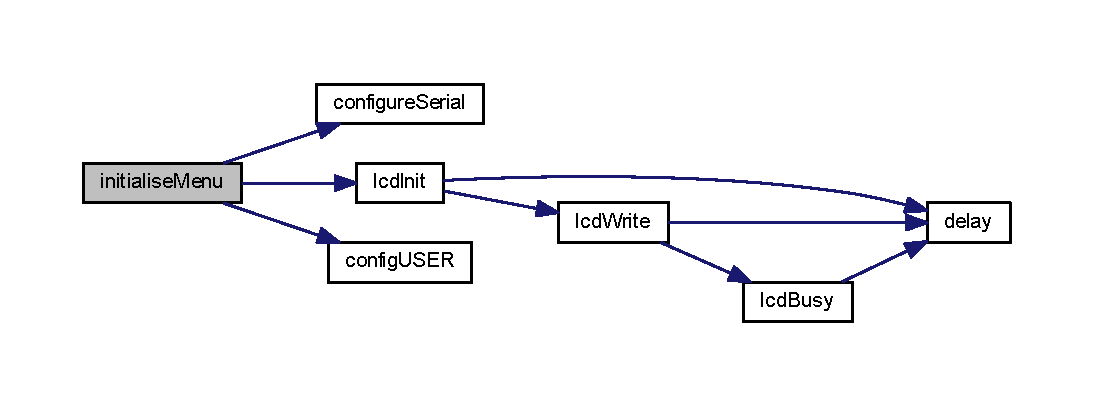
\includegraphics[width=350pt]{_menusystem2_8c_a94b96ccbb8f3c627c5d59189498a3c1b_cgraph}
\end{center}
\end{figure}


\hypertarget{_menusystem2_8c_a0f329206447b1f40e6f730b346aaaf44}{\index{Menusystem2.\+c@{Menusystem2.\+c}!menu\+I\+S\+R@{menu\+I\+S\+R}}
\index{menu\+I\+S\+R@{menu\+I\+S\+R}!Menusystem2.\+c@{Menusystem2.\+c}}
\subsubsection[{menu\+I\+S\+R}]{\setlength{\rightskip}{0pt plus 5cm}void menu\+I\+S\+R (
\begin{DoxyParamCaption}
\item[{void}]{}
\end{DoxyParamCaption}
)}}\label{_menusystem2_8c_a0f329206447b1f40e6f730b346aaaf44}


I\+S\+R function for the menu subsystem. 



 Function\+: \hyperlink{_menusystem2_8c_a0f329206447b1f40e6f730b346aaaf44}{menu\+I\+S\+R(void)}

Include\+: \hyperlink{_menusystem_8h}{Menusystem.\+h}

Description\+: services any interrupts associated with the menu system

Arguments\+: None

Returns\+: None 

Definition at line 126 of file Menusystem2.\+c.

\hypertarget{_menusystem2_8c_afc5a5c12a076ae6c7424df4f4124a521}{\index{Menusystem2.\+c@{Menusystem2.\+c}!service\+Menu@{service\+Menu}}
\index{service\+Menu@{service\+Menu}!Menusystem2.\+c@{Menusystem2.\+c}}
\subsubsection[{service\+Menu}]{\setlength{\rightskip}{0pt plus 5cm}void service\+Menu (
\begin{DoxyParamCaption}
\item[{void}]{}
\end{DoxyParamCaption}
)}}\label{_menusystem2_8c_afc5a5c12a076ae6c7424df4f4124a521}


services any user interface with the menu 



 Function\+: \hyperlink{_menusystem2_8c_afc5a5c12a076ae6c7424df4f4124a521}{service\+Menu(void)}

Include\+:

Description\+: Checks if the user has made any inputs to the system. If not the function simply returns. If they have then it services the inputs, displays the correct outputs and performs the specified actions

Arguments\+: None

Returns\+: None 

Definition at line 87 of file Menusystem2.\+c.



Here is the call graph for this function\+:\nopagebreak
\begin{figure}[H]
\begin{center}
\leavevmode
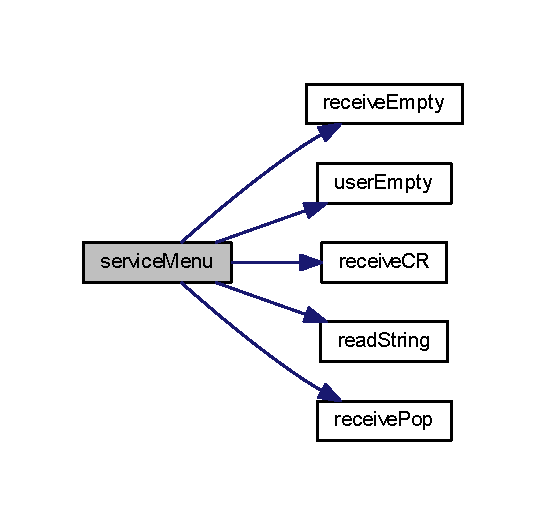
\includegraphics[width=262pt]{_menusystem2_8c_afc5a5c12a076ae6c7424df4f4124a521_cgraph}
\end{center}
\end{figure}



\hypertarget{newmain_8c}{\section{newmain.\+c File Reference}
\label{newmain_8c}\index{newmain.\+c@{newmain.\+c}}
}
{\ttfamily \#include \char`\"{}Common.\+h\char`\"{}}\\*
{\ttfamily \#include \char`\"{}Tracking.\+h\char`\"{}}\\*
{\ttfamily \#include \char`\"{}Range.\+h\char`\"{}}\\*
{\ttfamily \#include \char`\"{}User\+\_\+\+Interface.\+h\char`\"{}}\\*
{\ttfamily \#include \char`\"{}Serial.\+h\char`\"{}}\\*
{\ttfamily \#include \char`\"{}Pan\+Tilt.\+h\char`\"{}}\\*
{\ttfamily \#include \char`\"{}Menusystem.\+h\char`\"{}}\\*
Include dependency graph for newmain.\+c\+:\nopagebreak
\begin{figure}[H]
\begin{center}
\leavevmode
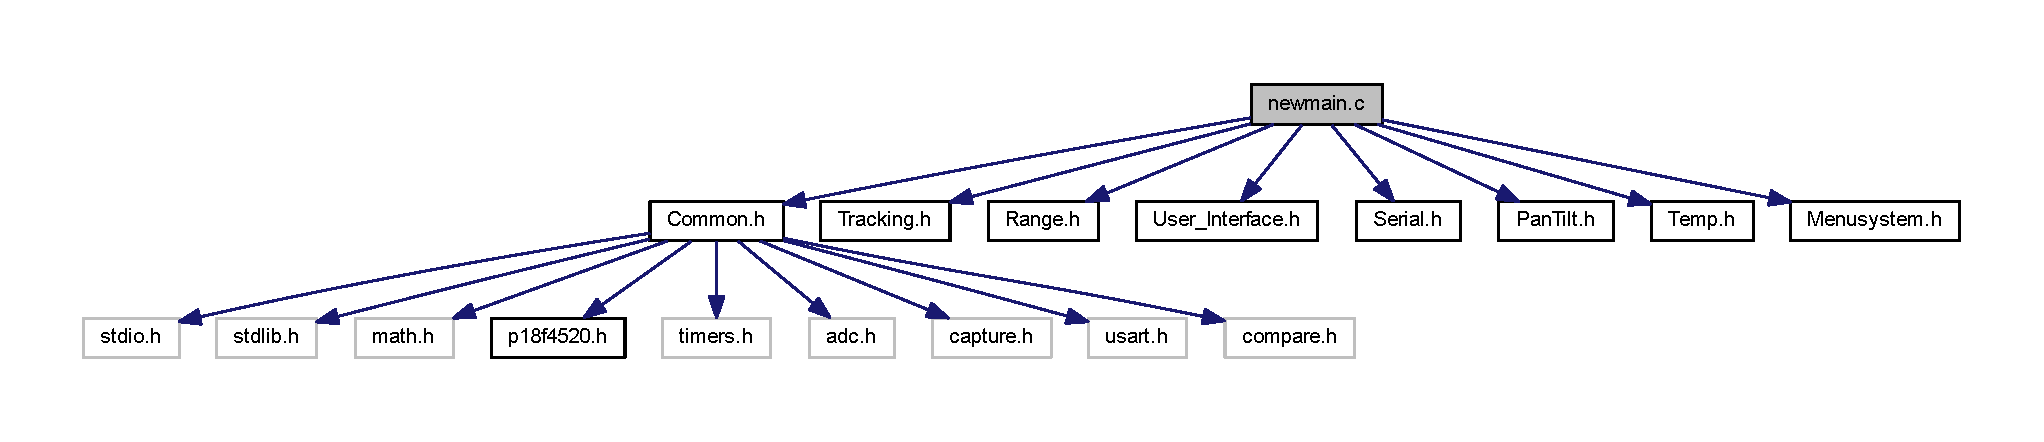
\includegraphics[width=350pt]{newmain_8c__incl}
\end{center}
\end{figure}
\subsection*{Functions}
\begin{DoxyCompactItemize}
\item 
void \hyperlink{newmain_8c_acdef7a1fd863a6d3770c1268cb06add3}{main} ()
\begin{DoxyCompactList}\small\item\em Program entry point. \end{DoxyCompactList}\end{DoxyCompactItemize}


\subsection{Function Documentation}
\hypertarget{newmain_8c_acdef7a1fd863a6d3770c1268cb06add3}{\index{newmain.\+c@{newmain.\+c}!main@{main}}
\index{main@{main}!newmain.\+c@{newmain.\+c}}
\subsubsection[{main}]{\setlength{\rightskip}{0pt plus 5cm}void main (
\begin{DoxyParamCaption}
{}
\end{DoxyParamCaption}
)}}\label{newmain_8c_acdef7a1fd863a6d3770c1268cb06add3}


Program entry point. 



 Function\+: \hyperlink{newmain_8c_acdef7a1fd863a6d3770c1268cb06add3}{main(void)}

Include\+: Local to \hyperlink{newmain_8c}{newmain.\+c}

Description\+: stores the current system state and manages all transitions

Arguments\+: None

Returns\+: None 

Definition at line 44 of file newmain.\+c.



Here is the call graph for this function\+:\nopagebreak
\begin{figure}[H]
\begin{center}
\leavevmode
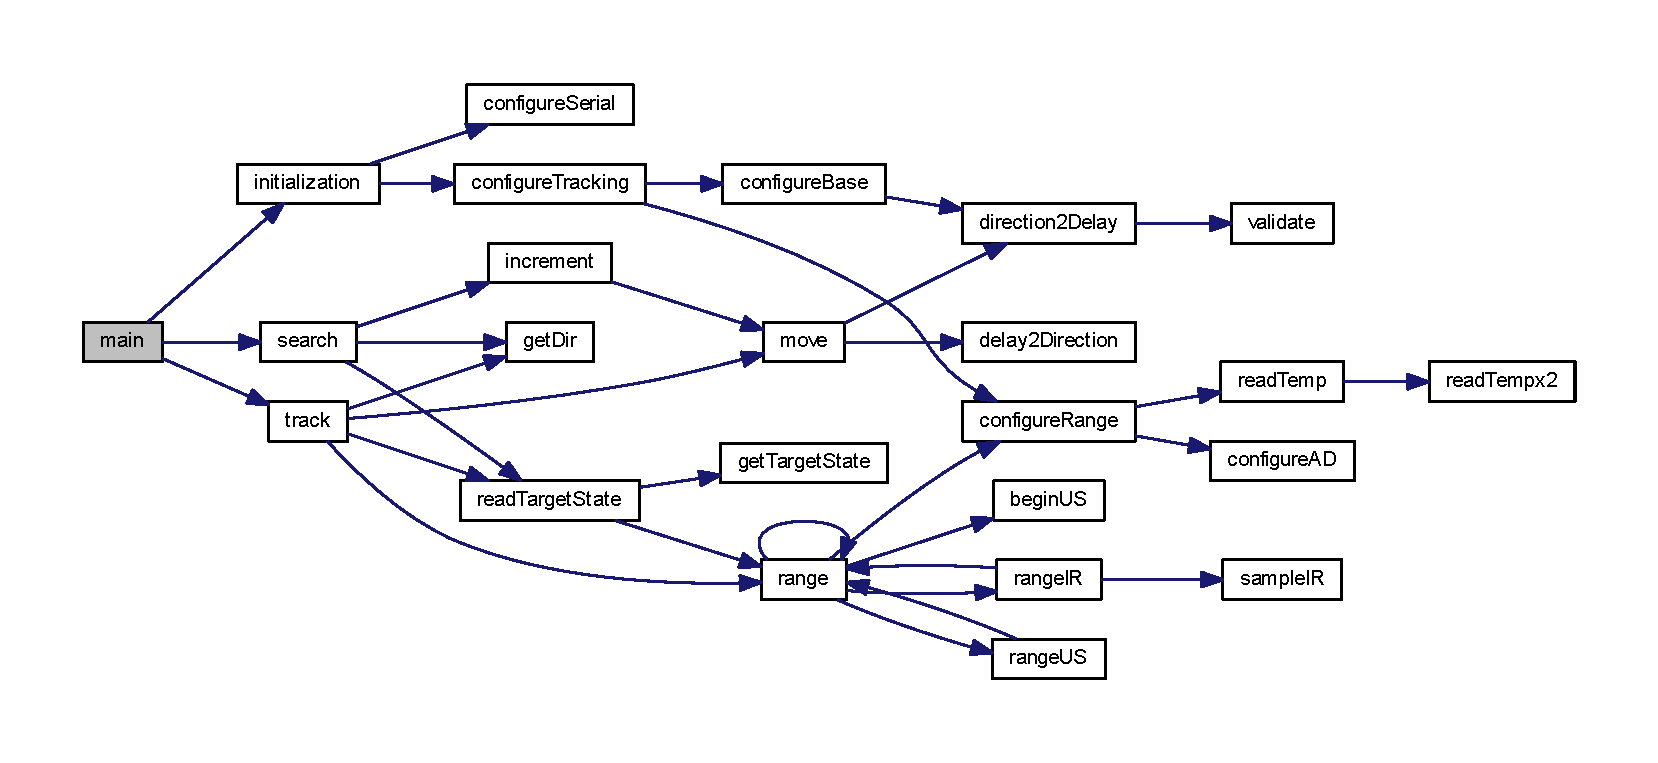
\includegraphics[width=350pt]{newmain_8c_acdef7a1fd863a6d3770c1268cb06add3_cgraph}
\end{center}
\end{figure}



\hypertarget{p18f4520_8h}{\section{p18f4520.\+h File Reference}
\label{p18f4520_8h}\index{p18f4520.\+h@{p18f4520.\+h}}
}
\subsection*{Macros}
\begin{DoxyCompactItemize}
\item 
\#define \hyperlink{p18f4520_8h_a321a20f839f3d9ccd0db1dc865850dc7}{A\+C\+C\+E\+S\+S}~0
\item 
\#define \hyperlink{p18f4520_8h_aa8480aed89a168ec484727f5ac985cd0}{B\+A\+N\+K\+E\+D}~1
\item 
\#define \hyperlink{p18f4520_8h_a153a328af535691126bf4955e5d896e6}{Nop}()~\{\+\_\+asm nop \+\_\+endasm\}
\item 
\#define \hyperlink{p18f4520_8h_afd3d2a511a2e746319056241f430ba70}{Clr\+Wdt}()~\{\+\_\+asm clrwdt \+\_\+endasm\}
\item 
\#define \hyperlink{p18f4520_8h_a97ff5dd2b06944ae9f9c916f2e03a1c6}{Sleep}()~\{\+\_\+asm sleep \+\_\+endasm\}
\item 
\#define \hyperlink{p18f4520_8h_a92b3099e50f63f0f06119e71a5ff2bab}{Reset}()~\{\+\_\+asm reset \+\_\+endasm\}
\item 
\#define \hyperlink{p18f4520_8h_abcb5b88260dabd5df8340d840bfdd404}{Rlcf}(f, dest, access)~\{\+\_\+asm movlb f rlcf f,dest,access \+\_\+endasm\}
\item 
\#define \hyperlink{p18f4520_8h_a05b76c712a339fc48cb8c88ef23b7f29}{Rlncf}(f, dest, access)~\{\+\_\+asm movlb f rlncf f,dest,access \+\_\+endasm\}
\item 
\#define \hyperlink{p18f4520_8h_a301a1cd412eaec5dce59535d9424f978}{Rrcf}(f, dest, access)~\{\+\_\+asm movlb f rrcf f,dest,access \+\_\+endasm\}
\item 
\#define \hyperlink{p18f4520_8h_a2a7d6d29a8b54c35bdd02744cd4bdedd}{Rrncf}(f, dest, access)~\{\+\_\+asm movlb f rrncf f,dest,access \+\_\+endasm\}
\item 
\#define \hyperlink{p18f4520_8h_a4e1f2584eeffe2692be70387a220d3ca}{Swapf}(f, dest, access)~\{\+\_\+asm movlb f swapf f,dest,access \+\_\+endasm \}
\item 
\#define \hyperlink{p18f4520_8h_a6fbafc3b67b7d1c9fb155337955dc9cc}{I\+N\+T\+S\+A\+V\+E\+L\+O\+C\+S}~\hyperlink{p18f4520_8h_a891a7dcc7cf8032dc2097f6acaf62527}{T\+B\+L\+P\+T\+R}, \hyperlink{p18f4520_8h_a1b036f387199c475c398f0d8e335256f}{T\+A\+B\+L\+A\+T}, \hyperlink{p18f4520_8h_a3c1ab73a0be354304b62d6106775c112}{P\+R\+O\+D}
\end{DoxyCompactItemize}
\subsection*{Variables}
\begin{DoxyCompactItemize}
\item 
volatile near unsigned char \hyperlink{p18f4520_8h_aebce362af37861eaae117b98643b1972}{P\+O\+R\+T\+A}
\item 
\begin{tabbing}
xx\=xx\=xx\=xx\=xx\=xx\=xx\=xx\=xx\=\kill
union \{\\
\>struct \{\\
\>\>unsigned \hyperlink{p18f4520_8h_af4aee82db0f331ec487c285162ad2080}{RA0}:1\\
\>\>unsigned \hyperlink{p18f4520_8h_aad482be2ea46f93c566836a5bacfe8fa}{RA1}:1\\
\>\>unsigned \hyperlink{p18f4520_8h_aca53d3d1278cccb09266cdfd28b3a228}{RA2}:1\\
\>\>unsigned \hyperlink{p18f4520_8h_a8f3ec177e486f325d3de3c056086a252}{RA3}:1\\
\>\>unsigned \hyperlink{p18f4520_8h_a5f92d429d1d98799d3eb06228f1aa981}{RA4}:1\\
\>\>unsigned \hyperlink{p18f4520_8h_aa9e7a4dcc7895d60622615c1907930ec}{RA5}:1\\
\>\>unsigned \hyperlink{p18f4520_8h_a3a0d1ef28657c29e7f6ca18daeaf9007}{RA6}:1\\
\>\>unsigned \hyperlink{p18f4520_8h_a01407df9dffc53b85b510d2b2449fa99}{RA7}:1\\
\>\} \\
\>struct \{\\
\>\>unsigned \hyperlink{p18f4520_8h_acd5ccd38d5007d7b253180bd0755dbac}{AN0}:1\\
\>\>unsigned \hyperlink{p18f4520_8h_a17755225f690c9f00f837c6938ba81cc}{AN1}:1\\
\>\>unsigned \hyperlink{p18f4520_8h_a18d58b8681fabb74a18fd33a14ebb116}{AN2}:1\\
\>\>unsigned \hyperlink{p18f4520_8h_a14c81bfd326b99cdae7874ea9d671fba}{AN3}:1\\
\>\>unsigned \hyperlink{p18f4520_8h_a1f4187dbf42dae32895e2ee4db134f52}{T0CKI}:1\\
\>\>unsigned \hyperlink{p18f4520_8h_af700bc8107240117fa803c81a6600e07}{AN4}:1\\
\>\>unsigned \hyperlink{p18f4520_8h_a7a7428023880050758655cc4c1651505}{OSC2}:1\\
\>\>unsigned \hyperlink{p18f4520_8h_ad344e03453a08d6215b891a285f3e93f}{OSC1}:1\\
\>\} \\
\>struct \{\\
\>\>unsigned \hyperlink{p18f4520_8h_adf71f3d8410c1f1dbbc96680a92c49af}{\_\_pad0\_\_}:2\\
\>\>unsigned \hyperlink{p18f4520_8h_a5dee21fef8c6fbb39654e487c0c8732c}{VREFN}:1\\
\>\>unsigned \hyperlink{p18f4520_8h_a5cdc473d8bab5d6d337bc1533cdf0adf}{VREFP}:1\\
\>\>unsigned \hyperlink{p18f4520_8h_acaf2d0924a107ec6e8d2e31febaf66f9}{\_\_pad1\_\_}:1\\
\>\>unsigned \hyperlink{p18f4520_8h_a51b2046af199afab022c5bfaa7d0c4cf}{SS}:1\\
\>\>unsigned \hyperlink{p18f4520_8h_a0a66dcac450a40b082c7bcc32a7fac00}{CLKO}:1\\
\>\>unsigned \hyperlink{p18f4520_8h_ada39cffa189ad48263065d469e9023fe}{CLKI}:1\\
\>\} \\
\>struct \{\\
\>\>unsigned \hyperlink{p18f4520_8h_adf71f3d8410c1f1dbbc96680a92c49af}{\_\_pad0\_\_}:2\\
\>\>unsigned \hyperlink{p18f4520_8h_aa73fc18f4b18ee8858ea91f2a470c298}{CVREF}:1\\
\>\>unsigned \hyperlink{p18f4520_8h_acaf2d0924a107ec6e8d2e31febaf66f9}{\_\_pad1\_\_}:2\\
\>\>unsigned \hyperlink{p18f4520_8h_a2f3c1348cf7620e948455d6c4f7bb70d}{NOT\_SS}:1\\
\>\} \\
\>struct \{\\
\>\>unsigned \hyperlink{p18f4520_8h_adf71f3d8410c1f1dbbc96680a92c49af}{\_\_pad0\_\_}:5\\
\>\>unsigned \hyperlink{p18f4520_8h_a6fc692566c00b7394eb73f86af0f1741}{LVDIN}:1\\
\>\} \\
\>struct \{\\
\>\>unsigned \hyperlink{p18f4520_8h_adf71f3d8410c1f1dbbc96680a92c49af}{\_\_pad0\_\_}:5\\
\>\>unsigned \hyperlink{p18f4520_8h_a862a19712c8b43e9b4735099301a2f78}{HLVDIN}:1\\
\>\} \\
\>struct \{\\
\>\>unsigned \hyperlink{p18f4520_8h_adf71f3d8410c1f1dbbc96680a92c49af}{\_\_pad0\_\_}:4\\
\>\>unsigned \hyperlink{p18f4520_8h_ac92ec38a908579dba4576b58d83b448b}{C1OUT}:1\\
\>\>unsigned \hyperlink{p18f4520_8h_a97b4baf2ebfd7bb4d0a6f4be6665c7ab}{C2OUT}:1\\
\>\} \\
\} \hyperlink{p18f4520_8h_a224dd3057b83148feebaae7563f388b2}{PORTAbits}\\

\end{tabbing}\item 
volatile near unsigned char \hyperlink{p18f4520_8h_a34337bc9ccb72db88e471fd229a2774e}{P\+O\+R\+T\+B}
\item 
\begin{tabbing}
xx\=xx\=xx\=xx\=xx\=xx\=xx\=xx\=xx\=\kill
union \{\\
\>struct \{\\
\>\>unsigned \hyperlink{p18f4520_8h_ad7a7c5386a08c77d293ac8de282bb7ee}{RB0}:1\\
\>\>unsigned \hyperlink{p18f4520_8h_a2dd83fe6920ad970c529af6a85f29917}{RB1}:1\\
\>\>unsigned \hyperlink{p18f4520_8h_acd7d4150f0717db56bb0849d8643a7ce}{RB2}:1\\
\>\>unsigned \hyperlink{p18f4520_8h_adfc0d406dbec0d9ad7e8e05d6b9e8dc6}{RB3}:1\\
\>\>unsigned \hyperlink{p18f4520_8h_a5ab7a1f43e97bcba0b28b5a32fcd8f2e}{RB4}:1\\
\>\>unsigned \hyperlink{p18f4520_8h_ab8751b90688e9e19f9e26131a9174150}{RB5}:1\\
\>\>unsigned \hyperlink{p18f4520_8h_a352d769bfd44cae31a5e9f836c70ddf3}{RB6}:1\\
\>\>unsigned \hyperlink{p18f4520_8h_a1e0c6dd8b0b71363366459af62cbaeaf}{RB7}:1\\
\>\} \\
\>struct \{\\
\>\>unsigned \hyperlink{p18f4520_8h_a61390f5d12eec8ec849e4a2bebeefcf1}{INT0}:1\\
\>\>unsigned \hyperlink{p18f4520_8h_a47cc5a5beb081340f905482dc80e00d3}{INT1}:1\\
\>\>unsigned \hyperlink{p18f4520_8h_a701a787be03bde234890290d2a507f1d}{INT2}:1\\
\>\>unsigned \hyperlink{p18f4520_8h_aadcf52da61805515302b2ccea19b97c1}{CCP2}:1\\
\>\>unsigned \hyperlink{p18f4520_8h_a594355c21c3dbe2030d535b160f7461c}{KBI0}:1\\
\>\>unsigned \hyperlink{p18f4520_8h_abdb433a8fa07b823ae40014d02840dde}{KBI1}:1\\
\>\>unsigned \hyperlink{p18f4520_8h_ae1fd527495c6fb60c4526acdeb2a4e76}{KBI2}:1\\
\>\>unsigned \hyperlink{p18f4520_8h_ae65e712a66fadf4042ca7b8f20f71d91}{KBI3}:1\\
\>\} \\
\>struct \{\\
\>\>unsigned \hyperlink{p18f4520_8h_a880c1731ebf7b50be6bea22d628e229b}{AN12}:1\\
\>\>unsigned \hyperlink{p18f4520_8h_ae0a7a141ad6c1774d504034fbb98c119}{AN10}:1\\
\>\>unsigned \hyperlink{p18f4520_8h_abbfae8cbd12f0a3d16923d2aaa521b7c}{AN8}:1\\
\>\>unsigned \hyperlink{p18f4520_8h_a0b73b0a8566abfb960e29b58ab23da23}{AN9}:1\\
\>\>unsigned \hyperlink{p18f4520_8h_aed8e36b52601048536412c6e71ef07aa}{AN11}:1\\
\>\>unsigned \hyperlink{p18f4520_8h_ad081c8f0410368b5d21309b334996ff9}{PGM}:1\\
\>\>unsigned \hyperlink{p18f4520_8h_a4a35c7b0ff0984a7b43e18df5b5831b7}{PGC}:1\\
\>\>unsigned \hyperlink{p18f4520_8h_ab097112b9258ab5f170f706c55636950}{PGD}:1\\
\>\} \\
\>struct \{\\
\>\>unsigned \hyperlink{p18f4520_8h_a7bd87769c4dc394148e6278c2c94e8b7}{FLT0}:1\\
\>\} \\
\} \hyperlink{p18f4520_8h_a48c59e09cbfcfac3f70c147e4fa95a0e}{PORTBbits}\\

\end{tabbing}\item 
volatile near unsigned char \hyperlink{p18f4520_8h_aa2304b29bba37fc0fedd4b28df6693cb}{P\+O\+R\+T\+C}
\item 
\begin{tabbing}
xx\=xx\=xx\=xx\=xx\=xx\=xx\=xx\=xx\=\kill
union \{\\
\>struct \{\\
\>\>unsigned \hyperlink{p18f4520_8h_a7ea5e081e0d3ea33ca014db57540107d}{RC0}:1\\
\>\>unsigned \hyperlink{p18f4520_8h_acbac2bc4f50222ec7e8549d800993842}{RC1}:1\\
\>\>unsigned \hyperlink{p18f4520_8h_a2155381890524f46a1a03878e5f52682}{RC2}:1\\
\>\>unsigned \hyperlink{p18f4520_8h_ae6cab3544e1e4b7eaec41046bf007800}{RC3}:1\\
\>\>unsigned \hyperlink{p18f4520_8h_aed6dec1d13dadc4721b39d5431fca93e}{RC4}:1\\
\>\>unsigned \hyperlink{p18f4520_8h_abc8b6cf48e22cac7c8a4e538ed7ae21f}{RC5}:1\\
\>\>unsigned \hyperlink{p18f4520_8h_a77078b289c7148a359992cfb7cd78a77}{RC6}:1\\
\>\>unsigned \hyperlink{p18f4520_8h_aed9978cb005f477085d029bb74779abf}{RC7}:1\\
\>\} \\
\>struct \{\\
\>\>unsigned \hyperlink{p18f4520_8h_a9cc28881e0fd26e5d42c2ee300ec8d67}{T1OSO}:1\\
\>\>unsigned \hyperlink{p18f4520_8h_a4cf89cfdf1d37209e3122ba98bba96b8}{T1OSI}:1\\
\>\>unsigned \hyperlink{p18f4520_8h_a5f6bb62b5208a9e5e26f93aa6e23be22}{CCP1}:1\\
\>\>unsigned \hyperlink{p18f4520_8h_a36f384b4a800e26f845d0ce615307d20}{SCK}:1\\
\>\>unsigned \hyperlink{p18f4520_8h_aa5136fd740c147383f4c6f896aab7220}{SDI}:1\\
\>\>unsigned \hyperlink{p18f4520_8h_ac54d1f23554dcbb4a5f23b777ef139e1}{SDO}:1\\
\>\>unsigned \hyperlink{p18f4520_8h_ac893df5d6253b8ce4a2657ecaf832a52}{TX}:1\\
\>\>unsigned \hyperlink{p18f4520_8h_a0edde991f780dcde0ab3e179203106db}{RX}:1\\
\>\} \\
\>struct \{\\
\>\>unsigned \hyperlink{p18f4520_8h_aa581a1c53e03c9b9cb48161475d913bb}{T13CKI}:1\\
\>\>unsigned \hyperlink{p18f4520_8h_aadcf52da61805515302b2ccea19b97c1}{CCP2}:1\\
\>\>unsigned \hyperlink{p18f4520_8h_adf71f3d8410c1f1dbbc96680a92c49af}{\_\_pad0\_\_}:1\\
\>\>unsigned \hyperlink{p18f4520_8h_ae8aa3179a42fb92cc1f2e7db1110b50f}{SCL}:1\\
\>\>unsigned \hyperlink{p18f4520_8h_aeb83d5b3d6554f917473b93470376916}{SDA}:1\\
\>\>unsigned \hyperlink{p18f4520_8h_acaf2d0924a107ec6e8d2e31febaf66f9}{\_\_pad1\_\_}:1\\
\>\>unsigned \hyperlink{p18f4520_8h_a1456ec5388b24920108c49ed74e00faa}{CK}:1\\
\>\>unsigned \hyperlink{p18f4520_8h_acc36376b7b880be90829176b77f20764}{DT}:1\\
\>\} \\
\>struct \{\\
\>\>unsigned \hyperlink{p18f4520_8h_adf02fd8be2d17f31eb1d38c7145b037a}{T1CKI}:1\\
\>\>unsigned \hyperlink{p18f4520_8h_adf71f3d8410c1f1dbbc96680a92c49af}{\_\_pad0\_\_}:1\\
\>\>unsigned \hyperlink{p18f4520_8h_a1a313ae8bf9fb89e2cfe37d04d521c79}{P1A}:1\\
\>\} \\
\} \hyperlink{p18f4520_8h_af1b30850f69fcdb90d5bcda81a6ffb57}{PORTCbits}\\

\end{tabbing}\item 
volatile near unsigned char \hyperlink{p18f4520_8h_ab81efa297900adba97f7eb5093c827d4}{P\+O\+R\+T\+D}
\item 
\begin{tabbing}
xx\=xx\=xx\=xx\=xx\=xx\=xx\=xx\=xx\=\kill
union \{\\
\>struct \{\\
\>\>unsigned \hyperlink{p18f4520_8h_a5e244c0d8c44f92adf1e3fa35b83ad7b}{RD0}:1\\
\>\>unsigned \hyperlink{p18f4520_8h_aaf160461556cf17b85f2e6210a87eec2}{RD1}:1\\
\>\>unsigned \hyperlink{p18f4520_8h_a8226de427632c18d70f0ba436e26848d}{RD2}:1\\
\>\>unsigned \hyperlink{p18f4520_8h_af17e8e4002cf3df68e9d78a35fd6c5fa}{RD3}:1\\
\>\>unsigned \hyperlink{p18f4520_8h_a1e1509ac90622f2daad1f47635a9632b}{RD4}:1\\
\>\>unsigned \hyperlink{p18f4520_8h_a69bfa549410c7235f9aaaeed9f406696}{RD5}:1\\
\>\>unsigned \hyperlink{p18f4520_8h_abafc54b5f1adc5ed88948f006088096e}{RD6}:1\\
\>\>unsigned \hyperlink{p18f4520_8h_a4b3e758ddc25f7b699b3410bf6a1c441}{RD7}:1\\
\>\} \\
\>struct \{\\
\>\>unsigned \hyperlink{p18f4520_8h_acc3ffaf2de5e9d812b23809704d4cbe0}{PSP0}:1\\
\>\>unsigned \hyperlink{p18f4520_8h_aad68a61d455727f7be404bbd8a84fc0f}{PSP1}:1\\
\>\>unsigned \hyperlink{p18f4520_8h_a664daf8a43e0cafde5db6594130ce9b4}{PSP2}:1\\
\>\>unsigned \hyperlink{p18f4520_8h_a3091ee9393441ed899dc4b5efbfa5ada}{PSP3}:1\\
\>\>unsigned \hyperlink{p18f4520_8h_afe9b186c96ecb85d86d2842d8ca876b1}{PSP4}:1\\
\>\>unsigned \hyperlink{p18f4520_8h_a1622f36583fed015c11c85c8ebf48b4c}{PSP5}:1\\
\>\>unsigned \hyperlink{p18f4520_8h_a39fcb989e0d079671fc860750b61c5bb}{PSP6}:1\\
\>\>unsigned \hyperlink{p18f4520_8h_a0dcf3dabbda2a0df676bd0f756d81101}{PSP7}:1\\
\>\} \\
\>struct \{\\
\>\>unsigned \hyperlink{p18f4520_8h_adf71f3d8410c1f1dbbc96680a92c49af}{\_\_pad0\_\_}:5\\
\>\>unsigned \hyperlink{p18f4520_8h_ab4a8558b14db40ef074602891fd2cce6}{P1B}:1\\
\>\>unsigned \hyperlink{p18f4520_8h_a4e3820d7b7cdd58bbb0ac74ceef61890}{P1C}:1\\
\>\>unsigned \hyperlink{p18f4520_8h_aef289ceabb3cd197479627036285208e}{P1D}:1\\
\>\} \\
\} \hyperlink{p18f4520_8h_aa1ea0be46cab4de464312aeabf9664c2}{PORTDbits}\\

\end{tabbing}\item 
volatile near unsigned char \hyperlink{p18f4520_8h_a2ab7ed3dd0dfcc8760bf8110f45ea3dc}{P\+O\+R\+T\+E}
\item 
\begin{tabbing}
xx\=xx\=xx\=xx\=xx\=xx\=xx\=xx\=xx\=\kill
union \{\\
\>struct \{\\
\>\>unsigned \hyperlink{p18f4520_8h_a2550355ab8702261c0eb3668ee1a98ca}{RE0}:1\\
\>\>unsigned \hyperlink{p18f4520_8h_ab0941b9fe283ded18d5c458ece7e5da8}{RE1}:1\\
\>\>unsigned \hyperlink{p18f4520_8h_a2c6937b597c6d7f887b9200f199491db}{RE2}:1\\
\>\>unsigned \hyperlink{p18f4520_8h_aa49256e650026bdf0e5a237b1aabdbb9}{RE3}:1\\
\>\} \\
\>struct \{\\
\>\>unsigned \hyperlink{p18f4520_8h_ae119f53c101ac632e338d91ab4a70e5f}{RD}:1\\
\>\>unsigned \hyperlink{p18f4520_8h_a93fc7151cdbe1259975f2d8b430a65ee}{WR}:1\\
\>\>unsigned \hyperlink{p18f4520_8h_af0e0138f849fddad3fc7e092822f224d}{CS}:1\\
\>\>unsigned \hyperlink{p18f4520_8h_a51b5e4c956502103067e4a967e0e3de1}{MCLR}:1\\
\>\} \\
\>struct \{\\
\>\>unsigned \hyperlink{p18f4520_8h_a4ba6c867f150eb12ee95c65e941dfdb0}{NOT\_RD}:1\\
\>\>unsigned \hyperlink{p18f4520_8h_a573e75e8be3fa55cbb28f89e2805dbfc}{NOT\_WR}:1\\
\>\>unsigned \hyperlink{p18f4520_8h_a973af192c1b5d23d6674b88132d4a49c}{NOT\_CS}:1\\
\>\>unsigned \hyperlink{p18f4520_8h_a12613522b8e364a793931812058ce492}{NOT\_MCLR}:1\\
\>\} \\
\>struct \{\\
\>\>unsigned \hyperlink{p18f4520_8h_a8fdd15532cd272aa4262ade69c9be01e}{AN5}:1\\
\>\>unsigned \hyperlink{p18f4520_8h_afaee1105a54449c269b62be8734f3ebd}{AN6}:1\\
\>\>unsigned \hyperlink{p18f4520_8h_a64648fddbfdf871c5d48221ee969230b}{AN7}:1\\
\>\>unsigned \hyperlink{p18f4520_8h_afcb04a73d5c9632048b396c5943c0a51}{VPP}:1\\
\>\} \\
\} \hyperlink{p18f4520_8h_a1da8b9f734eacb4c5660e4a4aa83aaa2}{PORTEbits}\\

\end{tabbing}\item 
volatile near unsigned char \hyperlink{p18f4520_8h_ad904cf1f621e7293f74afc934ff0b323}{L\+A\+T\+A}
\item 
\begin{tabbing}
xx\=xx\=xx\=xx\=xx\=xx\=xx\=xx\=xx\=\kill
struct \{\\
\>unsigned \hyperlink{p18f4520_8h_a6fcf9e0b57006985c36ba76fd7bc13d8}{LATA0}:1\\
\>unsigned \hyperlink{p18f4520_8h_a77e1a5f1eaa1f522e9d6f51fa3f4610c}{LATA1}:1\\
\>unsigned \hyperlink{p18f4520_8h_a4a36a70971ce7eae653077879fe88522}{LATA2}:1\\
\>unsigned \hyperlink{p18f4520_8h_a8eea54e1be8c153248bdc06bbdd5bcf1}{LATA3}:1\\
\>unsigned \hyperlink{p18f4520_8h_ac8eac35306eab37b11a4271107979af2}{LATA4}:1\\
\>unsigned \hyperlink{p18f4520_8h_a8aee660134772ea9145da72bd747d899}{LATA5}:1\\
\>unsigned \hyperlink{p18f4520_8h_ad1e58949c0d3d2f7b4de9624d2140ca2}{LATA6}:1\\
\>unsigned \hyperlink{p18f4520_8h_ae0dfbd26007eb663892e8ce0dbe13ca9}{LATA7}:1\\
\} \hyperlink{p18f4520_8h_ac049dd8a8caa9842c96bb677008b6c26}{LATAbits}\\

\end{tabbing}\item 
volatile near unsigned char \hyperlink{p18f4520_8h_a71cbfe6ab8619d64e6499e4ba5b54ae2}{L\+A\+T\+B}
\item 
\begin{tabbing}
xx\=xx\=xx\=xx\=xx\=xx\=xx\=xx\=xx\=\kill
struct \{\\
\>unsigned \hyperlink{p18f4520_8h_ad317da92846674694a76e7aae18614c0}{LATB0}:1\\
\>unsigned \hyperlink{p18f4520_8h_a857c4a989abd018efdba6755620c4e6a}{LATB1}:1\\
\>unsigned \hyperlink{p18f4520_8h_ab335d78b25b0a596f6f46daef1072f7f}{LATB2}:1\\
\>unsigned \hyperlink{p18f4520_8h_a6cd30f61f89a47fbbb9dc81d11448980}{LATB3}:1\\
\>unsigned \hyperlink{p18f4520_8h_a93b440c2c06c0bc97f2957f42ffaea29}{LATB4}:1\\
\>unsigned \hyperlink{p18f4520_8h_a501d0e6c952110b2b74aa37454736a8e}{LATB5}:1\\
\>unsigned \hyperlink{p18f4520_8h_a133ff1dad08c9cbfb6bccd0606076c6c}{LATB6}:1\\
\>unsigned \hyperlink{p18f4520_8h_aa052465171c5de5210a8cf1a2cb7fd91}{LATB7}:1\\
\} \hyperlink{p18f4520_8h_a18470066bda55b67c895768b1e4a0ffb}{LATBbits}\\

\end{tabbing}\item 
volatile near unsigned char \hyperlink{p18f4520_8h_a5a913e7460b2eb52aa8875f55aa74660}{L\+A\+T\+C}
\item 
\begin{tabbing}
xx\=xx\=xx\=xx\=xx\=xx\=xx\=xx\=xx\=\kill
struct \{\\
\>unsigned \hyperlink{p18f4520_8h_adc66a2aaebb22774ecf3b4a21d244de1}{LATC0}:1\\
\>unsigned \hyperlink{p18f4520_8h_aca64c17d86197b03c59989f652bf8b64}{LATC1}:1\\
\>unsigned \hyperlink{p18f4520_8h_a2a587811fb903e7f3e4462fd8d789df3}{LATC2}:1\\
\>unsigned \hyperlink{p18f4520_8h_a00c607221d4806a6d99270611ad8474f}{LATC3}:1\\
\>unsigned \hyperlink{p18f4520_8h_a552fc80c0dd1a68538a10e5711aa39fa}{LATC4}:1\\
\>unsigned \hyperlink{p18f4520_8h_a961a5b8f67e2a8ced4e856b84d6c10b0}{LATC5}:1\\
\>unsigned \hyperlink{p18f4520_8h_ab05632b9bb631f3716847bfa7134262d}{LATC6}:1\\
\>unsigned \hyperlink{p18f4520_8h_a794a52e672769f46981e0f49277709c0}{LATC7}:1\\
\} \hyperlink{p18f4520_8h_ab3402b6b3f47b0b4d9ac6e47b1da9ca0}{LATCbits}\\

\end{tabbing}\item 
volatile near unsigned char \hyperlink{p18f4520_8h_a72b17775f5801b80b6e3baa5a780d455}{L\+A\+T\+D}
\item 
\begin{tabbing}
xx\=xx\=xx\=xx\=xx\=xx\=xx\=xx\=xx\=\kill
struct \{\\
\>unsigned \hyperlink{p18f4520_8h_a3f4a63c62d2950aee9213b67ea17432d}{LATD0}:1\\
\>unsigned \hyperlink{p18f4520_8h_a34d889d674ac392ea95c63d29b3e4252}{LATD1}:1\\
\>unsigned \hyperlink{p18f4520_8h_adc54e366f4e7be344088482ec4c1e0c9}{LATD2}:1\\
\>unsigned \hyperlink{p18f4520_8h_a0023828564d9bb9f433a833399a2df15}{LATD3}:1\\
\>unsigned \hyperlink{p18f4520_8h_add23960d57e5315be05cac5860c8cc30}{LATD4}:1\\
\>unsigned \hyperlink{p18f4520_8h_a1cef346229e6bf6c3373e3368dc5f0d8}{LATD5}:1\\
\>unsigned \hyperlink{p18f4520_8h_a23e9fe369d39a1ce5a9f8fc6e221fc7b}{LATD6}:1\\
\>unsigned \hyperlink{p18f4520_8h_a60f7e492878d1ee2bcb037b5c41139fd}{LATD7}:1\\
\} \hyperlink{p18f4520_8h_a66ba0f73830772d37a0987c6d072fe67}{LATDbits}\\

\end{tabbing}\item 
volatile near unsigned char \hyperlink{p18f4520_8h_a509d41827bc3b2eaede5a36eefb6558f}{L\+A\+T\+E}
\item 
\begin{tabbing}
xx\=xx\=xx\=xx\=xx\=xx\=xx\=xx\=xx\=\kill
struct \{\\
\>unsigned \hyperlink{p18f4520_8h_a4136ff3de6a22d8ad71ba4b5c0773114}{LATE0}:1\\
\>unsigned \hyperlink{p18f4520_8h_aec27d2d6ea6ab19a25591d77f6e79876}{LATE1}:1\\
\>unsigned \hyperlink{p18f4520_8h_af21750f718f63a5901253e3731017a23}{LATE2}:1\\
\} \hyperlink{p18f4520_8h_a3a0e23b1c47a9adbe9b79b0efcf83092}{LATEbits}\\

\end{tabbing}\item 
volatile near unsigned char \hyperlink{p18f4520_8h_a22f2f0ea1ef95440c3dd0932d04bad9f}{D\+D\+R\+A}
\item 
\begin{tabbing}
xx\=xx\=xx\=xx\=xx\=xx\=xx\=xx\=xx\=\kill
union \{\\
\>struct \{\\
\>\>unsigned \hyperlink{p18f4520_8h_a5b058659efa978bacb96a404cfdbe610}{TRISA0}:1\\
\>\>unsigned \hyperlink{p18f4520_8h_ab129bf45a7e3be70a0acfea93d291273}{TRISA1}:1\\
\>\>unsigned \hyperlink{p18f4520_8h_af6281130cf7baba87c8550bd35d9d76d}{TRISA2}:1\\
\>\>unsigned \hyperlink{p18f4520_8h_a1a2488028e463b824d503f740b999146}{TRISA3}:1\\
\>\>unsigned \hyperlink{p18f4520_8h_a9f5eacb9cb6d29d89451ce640a6057ae}{TRISA4}:1\\
\>\>unsigned \hyperlink{p18f4520_8h_ae459cb825f88b23841a1fe1c65878399}{TRISA5}:1\\
\>\>unsigned \hyperlink{p18f4520_8h_a42bb066347a0919a8609bc10e28eb6c2}{TRISA6}:1\\
\>\>unsigned \hyperlink{p18f4520_8h_a41543e8aa038b05d2620c4808cef7023}{TRISA7}:1\\
\>\} \\
\>struct \{\\
\>\>unsigned \hyperlink{p18f4520_8h_af4aee82db0f331ec487c285162ad2080}{RA0}:1\\
\>\>unsigned \hyperlink{p18f4520_8h_aad482be2ea46f93c566836a5bacfe8fa}{RA1}:1\\
\>\>unsigned \hyperlink{p18f4520_8h_aca53d3d1278cccb09266cdfd28b3a228}{RA2}:1\\
\>\>unsigned \hyperlink{p18f4520_8h_a8f3ec177e486f325d3de3c056086a252}{RA3}:1\\
\>\>unsigned \hyperlink{p18f4520_8h_a5f92d429d1d98799d3eb06228f1aa981}{RA4}:1\\
\>\>unsigned \hyperlink{p18f4520_8h_aa9e7a4dcc7895d60622615c1907930ec}{RA5}:1\\
\>\>unsigned \hyperlink{p18f4520_8h_a3a0d1ef28657c29e7f6ca18daeaf9007}{RA6}:1\\
\>\>unsigned \hyperlink{p18f4520_8h_a01407df9dffc53b85b510d2b2449fa99}{RA7}:1\\
\>\} \\
\} \hyperlink{p18f4520_8h_a07566bce6071eff4ac8539b53199cb5e}{DDRAbits}\\

\end{tabbing}\item 
volatile near unsigned char \hyperlink{p18f4520_8h_a09522caca1ee06372c915b773f6b5bdd}{T\+R\+I\+S\+A}
\item 
\begin{tabbing}
xx\=xx\=xx\=xx\=xx\=xx\=xx\=xx\=xx\=\kill
union \{\\
\>struct \{\\
\>\>unsigned \hyperlink{p18f4520_8h_a5b058659efa978bacb96a404cfdbe610}{TRISA0}:1\\
\>\>unsigned \hyperlink{p18f4520_8h_ab129bf45a7e3be70a0acfea93d291273}{TRISA1}:1\\
\>\>unsigned \hyperlink{p18f4520_8h_af6281130cf7baba87c8550bd35d9d76d}{TRISA2}:1\\
\>\>unsigned \hyperlink{p18f4520_8h_a1a2488028e463b824d503f740b999146}{TRISA3}:1\\
\>\>unsigned \hyperlink{p18f4520_8h_a9f5eacb9cb6d29d89451ce640a6057ae}{TRISA4}:1\\
\>\>unsigned \hyperlink{p18f4520_8h_ae459cb825f88b23841a1fe1c65878399}{TRISA5}:1\\
\>\>unsigned \hyperlink{p18f4520_8h_a42bb066347a0919a8609bc10e28eb6c2}{TRISA6}:1\\
\>\>unsigned \hyperlink{p18f4520_8h_a41543e8aa038b05d2620c4808cef7023}{TRISA7}:1\\
\>\} \\
\>struct \{\\
\>\>unsigned \hyperlink{p18f4520_8h_af4aee82db0f331ec487c285162ad2080}{RA0}:1\\
\>\>unsigned \hyperlink{p18f4520_8h_aad482be2ea46f93c566836a5bacfe8fa}{RA1}:1\\
\>\>unsigned \hyperlink{p18f4520_8h_aca53d3d1278cccb09266cdfd28b3a228}{RA2}:1\\
\>\>unsigned \hyperlink{p18f4520_8h_a8f3ec177e486f325d3de3c056086a252}{RA3}:1\\
\>\>unsigned \hyperlink{p18f4520_8h_a5f92d429d1d98799d3eb06228f1aa981}{RA4}:1\\
\>\>unsigned \hyperlink{p18f4520_8h_aa9e7a4dcc7895d60622615c1907930ec}{RA5}:1\\
\>\>unsigned \hyperlink{p18f4520_8h_a3a0d1ef28657c29e7f6ca18daeaf9007}{RA6}:1\\
\>\>unsigned \hyperlink{p18f4520_8h_a01407df9dffc53b85b510d2b2449fa99}{RA7}:1\\
\>\} \\
\} \hyperlink{p18f4520_8h_ad9926229ce63683478163a7aad5ba4e4}{TRISAbits}\\

\end{tabbing}\item 
volatile near unsigned char \hyperlink{p18f4520_8h_aa549662b5988170c5ffdc4838d1fb7dc}{D\+D\+R\+B}
\item 
\begin{tabbing}
xx\=xx\=xx\=xx\=xx\=xx\=xx\=xx\=xx\=\kill
union \{\\
\>struct \{\\
\>\>unsigned \hyperlink{p18f4520_8h_a8c0a76a0dcde6d2328e831a289d6b087}{TRISB0}:1\\
\>\>unsigned \hyperlink{p18f4520_8h_a7db469569b510c735b7288bb4312c196}{TRISB1}:1\\
\>\>unsigned \hyperlink{p18f4520_8h_a6a9b5e42d2b7941caf83bfa1902dd9e9}{TRISB2}:1\\
\>\>unsigned \hyperlink{p18f4520_8h_afbf0db86e11d2b62309c7146bbf50a99}{TRISB3}:1\\
\>\>unsigned \hyperlink{p18f4520_8h_a3f9c4d0e1d77320b4ff08108cf8d7f82}{TRISB4}:1\\
\>\>unsigned \hyperlink{p18f4520_8h_a0d22aab025d01d88618a37bf366cd48d}{TRISB5}:1\\
\>\>unsigned \hyperlink{p18f4520_8h_ad0ca870291a16d4f8ebaca4230d42789}{TRISB6}:1\\
\>\>unsigned \hyperlink{p18f4520_8h_a9e73d3d0bb9a6ad9d46f2d162afc873d}{TRISB7}:1\\
\>\} \\
\>struct \{\\
\>\>unsigned \hyperlink{p18f4520_8h_ad7a7c5386a08c77d293ac8de282bb7ee}{RB0}:1\\
\>\>unsigned \hyperlink{p18f4520_8h_a2dd83fe6920ad970c529af6a85f29917}{RB1}:1\\
\>\>unsigned \hyperlink{p18f4520_8h_acd7d4150f0717db56bb0849d8643a7ce}{RB2}:1\\
\>\>unsigned \hyperlink{p18f4520_8h_adfc0d406dbec0d9ad7e8e05d6b9e8dc6}{RB3}:1\\
\>\>unsigned \hyperlink{p18f4520_8h_a5ab7a1f43e97bcba0b28b5a32fcd8f2e}{RB4}:1\\
\>\>unsigned \hyperlink{p18f4520_8h_ab8751b90688e9e19f9e26131a9174150}{RB5}:1\\
\>\>unsigned \hyperlink{p18f4520_8h_a352d769bfd44cae31a5e9f836c70ddf3}{RB6}:1\\
\>\>unsigned \hyperlink{p18f4520_8h_a1e0c6dd8b0b71363366459af62cbaeaf}{RB7}:1\\
\>\} \\
\} \hyperlink{p18f4520_8h_ad3eb78df900cf1eb84c4d0c5d9c21e82}{DDRBbits}\\

\end{tabbing}\item 
volatile near unsigned char \hyperlink{p18f4520_8h_a34c79aa37801a1c07caa6ffca946901f}{T\+R\+I\+S\+B}
\item 
\begin{tabbing}
xx\=xx\=xx\=xx\=xx\=xx\=xx\=xx\=xx\=\kill
union \{\\
\>struct \{\\
\>\>unsigned \hyperlink{p18f4520_8h_a8c0a76a0dcde6d2328e831a289d6b087}{TRISB0}:1\\
\>\>unsigned \hyperlink{p18f4520_8h_a7db469569b510c735b7288bb4312c196}{TRISB1}:1\\
\>\>unsigned \hyperlink{p18f4520_8h_a6a9b5e42d2b7941caf83bfa1902dd9e9}{TRISB2}:1\\
\>\>unsigned \hyperlink{p18f4520_8h_afbf0db86e11d2b62309c7146bbf50a99}{TRISB3}:1\\
\>\>unsigned \hyperlink{p18f4520_8h_a3f9c4d0e1d77320b4ff08108cf8d7f82}{TRISB4}:1\\
\>\>unsigned \hyperlink{p18f4520_8h_a0d22aab025d01d88618a37bf366cd48d}{TRISB5}:1\\
\>\>unsigned \hyperlink{p18f4520_8h_ad0ca870291a16d4f8ebaca4230d42789}{TRISB6}:1\\
\>\>unsigned \hyperlink{p18f4520_8h_a9e73d3d0bb9a6ad9d46f2d162afc873d}{TRISB7}:1\\
\>\} \\
\>struct \{\\
\>\>unsigned \hyperlink{p18f4520_8h_ad7a7c5386a08c77d293ac8de282bb7ee}{RB0}:1\\
\>\>unsigned \hyperlink{p18f4520_8h_a2dd83fe6920ad970c529af6a85f29917}{RB1}:1\\
\>\>unsigned \hyperlink{p18f4520_8h_acd7d4150f0717db56bb0849d8643a7ce}{RB2}:1\\
\>\>unsigned \hyperlink{p18f4520_8h_adfc0d406dbec0d9ad7e8e05d6b9e8dc6}{RB3}:1\\
\>\>unsigned \hyperlink{p18f4520_8h_a5ab7a1f43e97bcba0b28b5a32fcd8f2e}{RB4}:1\\
\>\>unsigned \hyperlink{p18f4520_8h_ab8751b90688e9e19f9e26131a9174150}{RB5}:1\\
\>\>unsigned \hyperlink{p18f4520_8h_a352d769bfd44cae31a5e9f836c70ddf3}{RB6}:1\\
\>\>unsigned \hyperlink{p18f4520_8h_a1e0c6dd8b0b71363366459af62cbaeaf}{RB7}:1\\
\>\} \\
\} \hyperlink{p18f4520_8h_a337110d58f6b0b5d27184b1736618061}{TRISBbits}\\

\end{tabbing}\item 
volatile near unsigned char \hyperlink{p18f4520_8h_a4e4c8d66239d98553e84b2ef3b47a1a2}{D\+D\+R\+C}
\item 
\begin{tabbing}
xx\=xx\=xx\=xx\=xx\=xx\=xx\=xx\=xx\=\kill
union \{\\
\>struct \{\\
\>\>unsigned \hyperlink{p18f4520_8h_a7139fc02fb7e183a323b496e5b3418ca}{TRISC0}:1\\
\>\>unsigned \hyperlink{p18f4520_8h_a1cc7a32e03a796eb4d05b85efe07ac2d}{TRISC1}:1\\
\>\>unsigned \hyperlink{p18f4520_8h_abd9996ec4b93a5c2879a5a305b2ddc32}{TRISC2}:1\\
\>\>unsigned \hyperlink{p18f4520_8h_a327dc42ea095c5655864fd2b5f23a6a6}{TRISC3}:1\\
\>\>unsigned \hyperlink{p18f4520_8h_af274ba23f40e654e5d022a3601a16389}{TRISC4}:1\\
\>\>unsigned \hyperlink{p18f4520_8h_ab595edfadebdcdf63ca82b8a697cc0f4}{TRISC5}:1\\
\>\>unsigned \hyperlink{p18f4520_8h_a51c0064b28fdaabb363e854fa607b36d}{TRISC6}:1\\
\>\>unsigned \hyperlink{p18f4520_8h_a0ab7b5e0075f615db54ad8f56118bf64}{TRISC7}:1\\
\>\} \\
\>struct \{\\
\>\>unsigned \hyperlink{p18f4520_8h_a7ea5e081e0d3ea33ca014db57540107d}{RC0}:1\\
\>\>unsigned \hyperlink{p18f4520_8h_acbac2bc4f50222ec7e8549d800993842}{RC1}:1\\
\>\>unsigned \hyperlink{p18f4520_8h_a2155381890524f46a1a03878e5f52682}{RC2}:1\\
\>\>unsigned \hyperlink{p18f4520_8h_ae6cab3544e1e4b7eaec41046bf007800}{RC3}:1\\
\>\>unsigned \hyperlink{p18f4520_8h_aed6dec1d13dadc4721b39d5431fca93e}{RC4}:1\\
\>\>unsigned \hyperlink{p18f4520_8h_abc8b6cf48e22cac7c8a4e538ed7ae21f}{RC5}:1\\
\>\>unsigned \hyperlink{p18f4520_8h_a77078b289c7148a359992cfb7cd78a77}{RC6}:1\\
\>\>unsigned \hyperlink{p18f4520_8h_aed9978cb005f477085d029bb74779abf}{RC7}:1\\
\>\} \\
\} \hyperlink{p18f4520_8h_a2b17e7018f773dc267a8842bc888df5f}{DDRCbits}\\

\end{tabbing}\item 
volatile near unsigned char \hyperlink{p18f4520_8h_a299caf58f2255f7e2347afa31e00cd9a}{T\+R\+I\+S\+C}
\item 
\begin{tabbing}
xx\=xx\=xx\=xx\=xx\=xx\=xx\=xx\=xx\=\kill
union \{\\
\>struct \{\\
\>\>unsigned \hyperlink{p18f4520_8h_a7139fc02fb7e183a323b496e5b3418ca}{TRISC0}:1\\
\>\>unsigned \hyperlink{p18f4520_8h_a1cc7a32e03a796eb4d05b85efe07ac2d}{TRISC1}:1\\
\>\>unsigned \hyperlink{p18f4520_8h_abd9996ec4b93a5c2879a5a305b2ddc32}{TRISC2}:1\\
\>\>unsigned \hyperlink{p18f4520_8h_a327dc42ea095c5655864fd2b5f23a6a6}{TRISC3}:1\\
\>\>unsigned \hyperlink{p18f4520_8h_af274ba23f40e654e5d022a3601a16389}{TRISC4}:1\\
\>\>unsigned \hyperlink{p18f4520_8h_ab595edfadebdcdf63ca82b8a697cc0f4}{TRISC5}:1\\
\>\>unsigned \hyperlink{p18f4520_8h_a51c0064b28fdaabb363e854fa607b36d}{TRISC6}:1\\
\>\>unsigned \hyperlink{p18f4520_8h_a0ab7b5e0075f615db54ad8f56118bf64}{TRISC7}:1\\
\>\} \\
\>struct \{\\
\>\>unsigned \hyperlink{p18f4520_8h_a7ea5e081e0d3ea33ca014db57540107d}{RC0}:1\\
\>\>unsigned \hyperlink{p18f4520_8h_acbac2bc4f50222ec7e8549d800993842}{RC1}:1\\
\>\>unsigned \hyperlink{p18f4520_8h_a2155381890524f46a1a03878e5f52682}{RC2}:1\\
\>\>unsigned \hyperlink{p18f4520_8h_ae6cab3544e1e4b7eaec41046bf007800}{RC3}:1\\
\>\>unsigned \hyperlink{p18f4520_8h_aed6dec1d13dadc4721b39d5431fca93e}{RC4}:1\\
\>\>unsigned \hyperlink{p18f4520_8h_abc8b6cf48e22cac7c8a4e538ed7ae21f}{RC5}:1\\
\>\>unsigned \hyperlink{p18f4520_8h_a77078b289c7148a359992cfb7cd78a77}{RC6}:1\\
\>\>unsigned \hyperlink{p18f4520_8h_aed9978cb005f477085d029bb74779abf}{RC7}:1\\
\>\} \\
\} \hyperlink{p18f4520_8h_a8b60042877226e0a6efa8e165cfe8452}{TRISCbits}\\

\end{tabbing}\item 
volatile near unsigned char \hyperlink{p18f4520_8h_aed4238a1472a90e43f6181ef668b773f}{D\+D\+R\+D}
\item 
\begin{tabbing}
xx\=xx\=xx\=xx\=xx\=xx\=xx\=xx\=xx\=\kill
union \{\\
\>struct \{\\
\>\>unsigned \hyperlink{p18f4520_8h_a02e71f0acc7d30edcc4265da7e1f304b}{TRISD0}:1\\
\>\>unsigned \hyperlink{p18f4520_8h_adfa57900d6ec4b87da98d854cc8ebf6a}{TRISD1}:1\\
\>\>unsigned \hyperlink{p18f4520_8h_a156c405a7dadcf0dbfb07cf4f60ddd63}{TRISD2}:1\\
\>\>unsigned \hyperlink{p18f4520_8h_a1ae081adf1f9d5e58bf84ded11b2579a}{TRISD3}:1\\
\>\>unsigned \hyperlink{p18f4520_8h_a79f0c732f439ef114017863c2d88f248}{TRISD4}:1\\
\>\>unsigned \hyperlink{p18f4520_8h_a067fbe843ef97f221b0562dca2c02d49}{TRISD5}:1\\
\>\>unsigned \hyperlink{p18f4520_8h_ac72e078f9449e51dfee0cdcfb14ac80a}{TRISD6}:1\\
\>\>unsigned \hyperlink{p18f4520_8h_a01348c49d0b9abaa2122fc6f44e020e3}{TRISD7}:1\\
\>\} \\
\>struct \{\\
\>\>unsigned \hyperlink{p18f4520_8h_a5e244c0d8c44f92adf1e3fa35b83ad7b}{RD0}:1\\
\>\>unsigned \hyperlink{p18f4520_8h_aaf160461556cf17b85f2e6210a87eec2}{RD1}:1\\
\>\>unsigned \hyperlink{p18f4520_8h_a8226de427632c18d70f0ba436e26848d}{RD2}:1\\
\>\>unsigned \hyperlink{p18f4520_8h_af17e8e4002cf3df68e9d78a35fd6c5fa}{RD3}:1\\
\>\>unsigned \hyperlink{p18f4520_8h_a1e1509ac90622f2daad1f47635a9632b}{RD4}:1\\
\>\>unsigned \hyperlink{p18f4520_8h_a69bfa549410c7235f9aaaeed9f406696}{RD5}:1\\
\>\>unsigned \hyperlink{p18f4520_8h_abafc54b5f1adc5ed88948f006088096e}{RD6}:1\\
\>\>unsigned \hyperlink{p18f4520_8h_a4b3e758ddc25f7b699b3410bf6a1c441}{RD7}:1\\
\>\} \\
\} \hyperlink{p18f4520_8h_a9ae91d7ff76e0c693d3e2d627698f7a7}{DDRDbits}\\

\end{tabbing}\item 
volatile near unsigned char \hyperlink{p18f4520_8h_a27fe1a8b121fc5461973401a85af2748}{T\+R\+I\+S\+D}
\item 
\begin{tabbing}
xx\=xx\=xx\=xx\=xx\=xx\=xx\=xx\=xx\=\kill
union \{\\
\>struct \{\\
\>\>unsigned \hyperlink{p18f4520_8h_a02e71f0acc7d30edcc4265da7e1f304b}{TRISD0}:1\\
\>\>unsigned \hyperlink{p18f4520_8h_adfa57900d6ec4b87da98d854cc8ebf6a}{TRISD1}:1\\
\>\>unsigned \hyperlink{p18f4520_8h_a156c405a7dadcf0dbfb07cf4f60ddd63}{TRISD2}:1\\
\>\>unsigned \hyperlink{p18f4520_8h_a1ae081adf1f9d5e58bf84ded11b2579a}{TRISD3}:1\\
\>\>unsigned \hyperlink{p18f4520_8h_a79f0c732f439ef114017863c2d88f248}{TRISD4}:1\\
\>\>unsigned \hyperlink{p18f4520_8h_a067fbe843ef97f221b0562dca2c02d49}{TRISD5}:1\\
\>\>unsigned \hyperlink{p18f4520_8h_ac72e078f9449e51dfee0cdcfb14ac80a}{TRISD6}:1\\
\>\>unsigned \hyperlink{p18f4520_8h_a01348c49d0b9abaa2122fc6f44e020e3}{TRISD7}:1\\
\>\} \\
\>struct \{\\
\>\>unsigned \hyperlink{p18f4520_8h_a5e244c0d8c44f92adf1e3fa35b83ad7b}{RD0}:1\\
\>\>unsigned \hyperlink{p18f4520_8h_aaf160461556cf17b85f2e6210a87eec2}{RD1}:1\\
\>\>unsigned \hyperlink{p18f4520_8h_a8226de427632c18d70f0ba436e26848d}{RD2}:1\\
\>\>unsigned \hyperlink{p18f4520_8h_af17e8e4002cf3df68e9d78a35fd6c5fa}{RD3}:1\\
\>\>unsigned \hyperlink{p18f4520_8h_a1e1509ac90622f2daad1f47635a9632b}{RD4}:1\\
\>\>unsigned \hyperlink{p18f4520_8h_a69bfa549410c7235f9aaaeed9f406696}{RD5}:1\\
\>\>unsigned \hyperlink{p18f4520_8h_abafc54b5f1adc5ed88948f006088096e}{RD6}:1\\
\>\>unsigned \hyperlink{p18f4520_8h_a4b3e758ddc25f7b699b3410bf6a1c441}{RD7}:1\\
\>\} \\
\} \hyperlink{p18f4520_8h_ac8912c59cdc684f141aba23277bd1900}{TRISDbits}\\

\end{tabbing}\item 
volatile near unsigned char \hyperlink{p18f4520_8h_af7a2e22f0be42260519acb8c7b4a4310}{D\+D\+R\+E}
\item 
\begin{tabbing}
xx\=xx\=xx\=xx\=xx\=xx\=xx\=xx\=xx\=\kill
union \{\\
\>struct \{\\
\>\>unsigned \hyperlink{p18f4520_8h_a4fde13ebb8ce91c1855d437b3e8721a1}{TRISE0}:1\\
\>\>unsigned \hyperlink{p18f4520_8h_ae3d523ca365d9db6485d2634660389fc}{TRISE1}:1\\
\>\>unsigned \hyperlink{p18f4520_8h_a9d223c63060ea30dfffa6cdb497772d8}{TRISE2}:1\\
\>\>unsigned \hyperlink{p18f4520_8h_adf71f3d8410c1f1dbbc96680a92c49af}{\_\_pad0\_\_}:1\\
\>\>unsigned \hyperlink{p18f4520_8h_a2ba12e7d20e86edff9f6ba4f3c25e2c3}{PSPMODE}:1\\
\>\>unsigned \hyperlink{p18f4520_8h_afa32b0a20f26513a6ab1b4e5351e32c5}{IBOV}:1\\
\>\>unsigned \hyperlink{p18f4520_8h_a4da1a0b0fcb9b0a285eda60937c3a8ec}{OBF}:1\\
\>\>unsigned \hyperlink{p18f4520_8h_abe5c97dbd24e0db1b78172b68f9efaf0}{IBF}:1\\
\>\} \\
\>struct \{\\
\>\>unsigned \hyperlink{p18f4520_8h_a2550355ab8702261c0eb3668ee1a98ca}{RE0}:1\\
\>\>unsigned \hyperlink{p18f4520_8h_ab0941b9fe283ded18d5c458ece7e5da8}{RE1}:1\\
\>\>unsigned \hyperlink{p18f4520_8h_a2c6937b597c6d7f887b9200f199491db}{RE2}:1\\
\>\>unsigned \hyperlink{p18f4520_8h_aa49256e650026bdf0e5a237b1aabdbb9}{RE3}:1\\
\>\} \\
\} \hyperlink{p18f4520_8h_ab2be6ac4367d760e36d5ea1f8fe8b5f8}{DDREbits}\\

\end{tabbing}\item 
volatile near unsigned char \hyperlink{p18f4520_8h_aee95800c3b0bf2debf149637d8458d7a}{T\+R\+I\+S\+E}
\item 
\begin{tabbing}
xx\=xx\=xx\=xx\=xx\=xx\=xx\=xx\=xx\=\kill
union \{\\
\>struct \{\\
\>\>unsigned \hyperlink{p18f4520_8h_a4fde13ebb8ce91c1855d437b3e8721a1}{TRISE0}:1\\
\>\>unsigned \hyperlink{p18f4520_8h_ae3d523ca365d9db6485d2634660389fc}{TRISE1}:1\\
\>\>unsigned \hyperlink{p18f4520_8h_a9d223c63060ea30dfffa6cdb497772d8}{TRISE2}:1\\
\>\>unsigned \hyperlink{p18f4520_8h_adf71f3d8410c1f1dbbc96680a92c49af}{\_\_pad0\_\_}:1\\
\>\>unsigned \hyperlink{p18f4520_8h_a2ba12e7d20e86edff9f6ba4f3c25e2c3}{PSPMODE}:1\\
\>\>unsigned \hyperlink{p18f4520_8h_afa32b0a20f26513a6ab1b4e5351e32c5}{IBOV}:1\\
\>\>unsigned \hyperlink{p18f4520_8h_a4da1a0b0fcb9b0a285eda60937c3a8ec}{OBF}:1\\
\>\>unsigned \hyperlink{p18f4520_8h_abe5c97dbd24e0db1b78172b68f9efaf0}{IBF}:1\\
\>\} \\
\>struct \{\\
\>\>unsigned \hyperlink{p18f4520_8h_a2550355ab8702261c0eb3668ee1a98ca}{RE0}:1\\
\>\>unsigned \hyperlink{p18f4520_8h_ab0941b9fe283ded18d5c458ece7e5da8}{RE1}:1\\
\>\>unsigned \hyperlink{p18f4520_8h_a2c6937b597c6d7f887b9200f199491db}{RE2}:1\\
\>\>unsigned \hyperlink{p18f4520_8h_aa49256e650026bdf0e5a237b1aabdbb9}{RE3}:1\\
\>\} \\
\} \hyperlink{p18f4520_8h_a0ddf7c90dd26f289221d98d661c67461}{TRISEbits}\\

\end{tabbing}\item 
volatile near unsigned char \hyperlink{p18f4520_8h_ab8cb9a5032e6a45aa72d1dc4c40209ba}{O\+S\+C\+T\+U\+N\+E}
\item 
\begin{tabbing}
xx\=xx\=xx\=xx\=xx\=xx\=xx\=xx\=xx\=\kill
union \{\\
\>struct \{\\
\>\>unsigned \hyperlink{p18f4520_8h_a11fb3128ca98255697c41d6e1e544a7f}{TUN}:5\\
\>\>unsigned \hyperlink{p18f4520_8h_adf71f3d8410c1f1dbbc96680a92c49af}{\_\_pad0\_\_}:1\\
\>\>unsigned \hyperlink{p18f4520_8h_a6c0e63e6845424ffd00b208f485d0b96}{PLLEN}:1\\
\>\>unsigned \hyperlink{p18f4520_8h_a5c64dbba7d65e4a97be0320050326d88}{INTSRC}:1\\
\>\} \\
\>struct \{\\
\>\>unsigned \hyperlink{p18f4520_8h_a33be6faef5c18356934f47fb28cfbed4}{TUN0}:1\\
\>\>unsigned \hyperlink{p18f4520_8h_aa4ccc91073c67d3d9e7d671acf89dea4}{TUN1}:1\\
\>\>unsigned \hyperlink{p18f4520_8h_a64dc8d1163082fd31503c0d5c30c1258}{TUN2}:1\\
\>\>unsigned \hyperlink{p18f4520_8h_acdf35316973ec0ba36c0e450dd796551}{TUN3}:1\\
\>\>unsigned \hyperlink{p18f4520_8h_aa6160c4f9517755d65ff45e469ab37c4}{TUN4}:1\\
\>\} \\
\} \hyperlink{p18f4520_8h_a88ceae0307237898c0988d570d281f1d}{OSCTUNEbits}\\

\end{tabbing}\item 
volatile near unsigned char \hyperlink{p18f4520_8h_a6c8d1aa73461b96916df6df31a289c2e}{P\+I\+E1}
\item 
\begin{tabbing}
xx\=xx\=xx\=xx\=xx\=xx\=xx\=xx\=xx\=\kill
struct \{\\
\>unsigned \hyperlink{p18f4520_8h_a41b95c767b7f4f9d788d421633333f25}{TMR1IE}:1\\
\>unsigned \hyperlink{p18f4520_8h_a2616057e89e17857a0232b45825b8a4a}{TMR2IE}:1\\
\>unsigned \hyperlink{p18f4520_8h_a25d4adacdc481717b9c89f8352bc4bc6}{CCP1IE}:1\\
\>unsigned \hyperlink{p18f4520_8h_acf24cc2186d69e72711aea0c30b99228}{SSPIE}:1\\
\>unsigned \hyperlink{p18f4520_8h_ae7b3b4752a0a4b6c084f1599ea98e724}{TXIE}:1\\
\>unsigned \hyperlink{p18f4520_8h_a756f5bf99764eb500a4a22b0693efb03}{RCIE}:1\\
\>unsigned \hyperlink{p18f4520_8h_ace69098082b2fd1d0929e31e71c1d5a9}{ADIE}:1\\
\>unsigned \hyperlink{p18f4520_8h_ac6ac1c31c48d67dda957637759523050}{PSPIE}:1\\
\} \hyperlink{p18f4520_8h_a0da258d430dd4e57d8f750549f9ee883}{PIE1bits}\\

\end{tabbing}\item 
volatile near unsigned char \hyperlink{p18f4520_8h_a9ebeed68820ca7eeead73b33b32ea46f}{P\+I\+R1}
\item 
\begin{tabbing}
xx\=xx\=xx\=xx\=xx\=xx\=xx\=xx\=xx\=\kill
struct \{\\
\>unsigned \hyperlink{p18f4520_8h_a1ca0d1f4b314bcc9d4a42d92d4512118}{TMR1IF}:1\\
\>unsigned \hyperlink{p18f4520_8h_a3e1791e78ad5d0e6b89e44e50c74f2c6}{TMR2IF}:1\\
\>unsigned \hyperlink{p18f4520_8h_a6daa84b9e3f6496da3121a80506f444e}{CCP1IF}:1\\
\>unsigned \hyperlink{p18f4520_8h_a8001253a95878a1eab217642803eb655}{SSPIF}:1\\
\>unsigned \hyperlink{p18f4520_8h_a045c6555e7e82fcf68e608d4404fb9ed}{TXIF}:1\\
\>unsigned \hyperlink{p18f4520_8h_a8ff1127552738fc483a7e1887045e8d2}{RCIF}:1\\
\>unsigned \hyperlink{p18f4520_8h_aca1613e7087914be4d69c5770eb8f4a3}{ADIF}:1\\
\>unsigned \hyperlink{p18f4520_8h_a20afb0effc6257b832464dcc7b574b52}{PSPIF}:1\\
\} \hyperlink{p18f4520_8h_ac4d6310cb479c743b217189b91114508}{PIR1bits}\\

\end{tabbing}\item 
volatile near unsigned char \hyperlink{p18f4520_8h_a809e3fefa5260e2e32b99582138ec56d}{I\+P\+R1}
\item 
\begin{tabbing}
xx\=xx\=xx\=xx\=xx\=xx\=xx\=xx\=xx\=\kill
struct \{\\
\>unsigned \hyperlink{p18f4520_8h_af67538f123f34dba63f2d7fd117b81b8}{TMR1IP}:1\\
\>unsigned \hyperlink{p18f4520_8h_aa206abb3a7302e7a14093148517120b5}{TMR2IP}:1\\
\>unsigned \hyperlink{p18f4520_8h_a22e018dfd301aac0bc39c9888c3b966e}{CCP1IP}:1\\
\>unsigned \hyperlink{p18f4520_8h_aedff60f34d8c46679fb3838766e41382}{SSPIP}:1\\
\>unsigned \hyperlink{p18f4520_8h_a7c083153541c7945b89d37fafb382767}{TXIP}:1\\
\>unsigned \hyperlink{p18f4520_8h_a3b093ee22d06f66ad6746bdb7487906c}{RCIP}:1\\
\>unsigned \hyperlink{p18f4520_8h_a8f421971631ed77d8709f9f11153aca5}{ADIP}:1\\
\>unsigned \hyperlink{p18f4520_8h_ae8c7e5bda8c02a6e922956cfb3888f9f}{PSPIP}:1\\
\} \hyperlink{p18f4520_8h_ac5992cad6272cf8f7b2b276f10ce6df5}{IPR1bits}\\

\end{tabbing}\item 
volatile near unsigned char \hyperlink{p18f4520_8h_a57f991b792677257a38e6e7ee9117c51}{P\+I\+E2}
\item 
\begin{tabbing}
xx\=xx\=xx\=xx\=xx\=xx\=xx\=xx\=xx\=\kill
union \{\\
\>struct \{\\
\>\>unsigned \hyperlink{p18f4520_8h_af032cd1ef97761506102829f69feb189}{CCP2IE}:1\\
\>\>unsigned \hyperlink{p18f4520_8h_a0f9cc64ee6e86633138b4e186eae33e2}{TMR3IE}:1\\
\>\>unsigned \hyperlink{p18f4520_8h_a33def5adb0eb28dc117daa857af96881}{HLVDIE}:1\\
\>\>unsigned \hyperlink{p18f4520_8h_aae975fe98fee9b9a8c3beaa9964bbc8f}{BCLIE}:1\\
\>\>unsigned \hyperlink{p18f4520_8h_add79ca08a8a158091c24636735fc5be0}{EEIE}:1\\
\>\>unsigned \hyperlink{p18f4520_8h_adf71f3d8410c1f1dbbc96680a92c49af}{\_\_pad0\_\_}:1\\
\>\>unsigned \hyperlink{p18f4520_8h_a70cc4783b21697eebf908893e71374f8}{CMIE}:1\\
\>\>unsigned \hyperlink{p18f4520_8h_abefe0ee693634a60897b07e3213094b5}{OSCFIE}:1\\
\>\} \\
\>struct \{\\
\>\>unsigned \hyperlink{p18f4520_8h_adf71f3d8410c1f1dbbc96680a92c49af}{\_\_pad0\_\_}:2\\
\>\>unsigned \hyperlink{p18f4520_8h_a957b8cf8198b7ca9c30cf9c730960a94}{LVDIE}:1\\
\>\} \\
\} \hyperlink{p18f4520_8h_a814d5739b0e69dd2026d5e2a82a93cde}{PIE2bits}\\

\end{tabbing}\item 
volatile near unsigned char \hyperlink{p18f4520_8h_a592c034286e84899cd4def5ab614c0c0}{P\+I\+R2}
\item 
\begin{tabbing}
xx\=xx\=xx\=xx\=xx\=xx\=xx\=xx\=xx\=\kill
union \{\\
\>struct \{\\
\>\>unsigned \hyperlink{p18f4520_8h_a7d689151681a8a50c953ecefd618eeb4}{CCP2IF}:1\\
\>\>unsigned \hyperlink{p18f4520_8h_a3543e05a68f8aaf308e3abf391109a47}{TMR3IF}:1\\
\>\>unsigned \hyperlink{p18f4520_8h_aea35961e5e13accb38ada5235641aac3}{HLVDIF}:1\\
\>\>unsigned \hyperlink{p18f4520_8h_a903514afa08123232b8209785a448348}{BCLIF}:1\\
\>\>unsigned \hyperlink{p18f4520_8h_a2daeaaf315ee9aa42f23a1eead2ae30c}{EEIF}:1\\
\>\>unsigned \hyperlink{p18f4520_8h_adf71f3d8410c1f1dbbc96680a92c49af}{\_\_pad0\_\_}:1\\
\>\>unsigned \hyperlink{p18f4520_8h_a36bdd9fcc72215b60877d39e7559d891}{CMIF}:1\\
\>\>unsigned \hyperlink{p18f4520_8h_a9b1676b34914c00fd91100f0928afcd5}{OSCFIF}:1\\
\>\} \\
\>struct \{\\
\>\>unsigned \hyperlink{p18f4520_8h_adf71f3d8410c1f1dbbc96680a92c49af}{\_\_pad0\_\_}:2\\
\>\>unsigned \hyperlink{p18f4520_8h_a7eed8d56af8d3063c286adba368d8dff}{LVDIF}:1\\
\>\} \\
\} \hyperlink{p18f4520_8h_a390de697cff026cc2b7b68fa8f97b9ea}{PIR2bits}\\

\end{tabbing}\item 
volatile near unsigned char \hyperlink{p18f4520_8h_ace430232489dfdca0f65cdcb926f6c5f}{I\+P\+R2}
\item 
\begin{tabbing}
xx\=xx\=xx\=xx\=xx\=xx\=xx\=xx\=xx\=\kill
union \{\\
\>struct \{\\
\>\>unsigned \hyperlink{p18f4520_8h_a618689042a4bab551d487f5e1d0f3053}{CCP2IP}:1\\
\>\>unsigned \hyperlink{p18f4520_8h_aad57646e4f713b57700063bf945b3d6d}{TMR3IP}:1\\
\>\>unsigned \hyperlink{p18f4520_8h_a17237c3a9b5296c80b9e776309a92bdb}{HLVDIP}:1\\
\>\>unsigned \hyperlink{p18f4520_8h_a08d03dc85ed3d3b47385b7fdd779bed5}{BCLIP}:1\\
\>\>unsigned \hyperlink{p18f4520_8h_a58b2791b877205cc0f0265a2181ed566}{EEIP}:1\\
\>\>unsigned \hyperlink{p18f4520_8h_adf71f3d8410c1f1dbbc96680a92c49af}{\_\_pad0\_\_}:1\\
\>\>unsigned \hyperlink{p18f4520_8h_aa8ee3d17a5a19c4d69285da5a18d1044}{CMIP}:1\\
\>\>unsigned \hyperlink{p18f4520_8h_a722e28d30422c0546433742170962d13}{OSCFIP}:1\\
\>\} \\
\>struct \{\\
\>\>unsigned \hyperlink{p18f4520_8h_adf71f3d8410c1f1dbbc96680a92c49af}{\_\_pad0\_\_}:2\\
\>\>unsigned \hyperlink{p18f4520_8h_a9a199ce940be797c493fda58d99cc817}{LVDIP}:1\\
\>\} \\
\} \hyperlink{p18f4520_8h_a735eca10981003c8a947e3ef29b391a7}{IPR2bits}\\

\end{tabbing}\item 
volatile near unsigned char \hyperlink{p18f4520_8h_adfa605b9cbaf14a24a63b34567711a26}{E\+E\+C\+O\+N1}
\item 
\begin{tabbing}
xx\=xx\=xx\=xx\=xx\=xx\=xx\=xx\=xx\=\kill
struct \{\\
\>unsigned \hyperlink{p18f4520_8h_ae119f53c101ac632e338d91ab4a70e5f}{RD}:1\\
\>unsigned \hyperlink{p18f4520_8h_a93fc7151cdbe1259975f2d8b430a65ee}{WR}:1\\
\>unsigned \hyperlink{p18f4520_8h_a8615dca9fd990870b04c31a53bdd72c4}{WREN}:1\\
\>unsigned \hyperlink{p18f4520_8h_a3bb4589054cd59f1b8572d6a902d95ff}{WRERR}:1\\
\>unsigned \hyperlink{p18f4520_8h_a9a6e110858d90b9659e53aacbda20998}{FREE}:1\\
\>unsigned \hyperlink{p18f4520_8h_adf71f3d8410c1f1dbbc96680a92c49af}{\_\_pad0\_\_}:1\\
\>unsigned \hyperlink{p18f4520_8h_afd04a41aad540f92aea41ffcc06b3c66}{CFGS}:1\\
\>unsigned \hyperlink{p18f4520_8h_a13b1895eb9a22342d108cdb7dbbe3cd0}{EEPGD}:1\\
\} \hyperlink{p18f4520_8h_a3000c48e2ebae2882bff2d81d5d1b3cb}{EECON1bits}\\

\end{tabbing}\item 
volatile near unsigned char \hyperlink{p18f4520_8h_a454333f5383f2a780f6b5acfa17acc50}{E\+E\+C\+O\+N2}
\item 
volatile near unsigned char \hyperlink{p18f4520_8h_ad8413bb9df2bbb28e8cb1640ca9923f6}{E\+E\+D\+A\+T\+A}
\item 
volatile near unsigned char \hyperlink{p18f4520_8h_a96dbfba90b9ab55ffb57f0a66ebb26a3}{E\+E\+A\+D\+R}
\item 
volatile near unsigned char \hyperlink{p18f4520_8h_add12983ed854a3cb280ad478e9a39a77}{R\+C\+S\+T\+A}
\item 
\begin{tabbing}
xx\=xx\=xx\=xx\=xx\=xx\=xx\=xx\=xx\=\kill
union \{\\
\>struct \{\\
\>\>unsigned \hyperlink{p18f4520_8h_ac31fb2fbd7c32147f4b24ba09b3e1ec7}{RX9D}:1\\
\>\>unsigned \hyperlink{p18f4520_8h_a51850c0a0e36c88695788d8258825fb1}{OERR}:1\\
\>\>unsigned \hyperlink{p18f4520_8h_a6e9c49ea6356906ea25431c922eb7c71}{FERR}:1\\
\>\>unsigned \hyperlink{p18f4520_8h_aa4d6c69beac6d542ad6bc014875fdff2}{ADDEN}:1\\
\>\>unsigned \hyperlink{p18f4520_8h_a078127b7efe1ed08283c57df8011d236}{CREN}:1\\
\>\>unsigned \hyperlink{p18f4520_8h_aad6c74492c60f7482e29b665c597b4c4}{SREN}:1\\
\>\>unsigned \hyperlink{p18f4520_8h_a3c20e41177e72cad42760612b44721c8}{RX9}:1\\
\>\>unsigned \hyperlink{p18f4520_8h_aae3b8a7f631dbd1d869a4f5491912a1d}{SPEN}:1\\
\>\} \\
\>struct \{\\
\>\>unsigned \hyperlink{p18f4520_8h_adf71f3d8410c1f1dbbc96680a92c49af}{\_\_pad0\_\_}:3\\
\>\>unsigned \hyperlink{p18f4520_8h_aab29c283a4eabe94288a5f297b336c91}{ADEN}:1\\
\>\} \\
\} \hyperlink{p18f4520_8h_a447d00268cf154c92255924f104ae3cc}{RCSTAbits}\\

\end{tabbing}\item 
volatile near unsigned char \hyperlink{p18f4520_8h_a101d567e89c66ec4da9b3d5258e42b76}{T\+X\+S\+T\+A}
\item 
\begin{tabbing}
xx\=xx\=xx\=xx\=xx\=xx\=xx\=xx\=xx\=\kill
struct \{\\
\>unsigned \hyperlink{p18f4520_8h_a220a1af7ce3aa239d66141ca4d1da879}{TX9D}:1\\
\>unsigned \hyperlink{p18f4520_8h_a63ff36fd0aa1645fb63d427eb941f177}{TRMT}:1\\
\>unsigned \hyperlink{p18f4520_8h_a5ac4f749c73f2dfc0f8699b73fe251fc}{BRGH}:1\\
\>unsigned \hyperlink{p18f4520_8h_a383a4f9d333362e925fdbaeed666c0fe}{SENDB}:1\\
\>unsigned \hyperlink{p18f4520_8h_aa0c7d775857a750168e34d810724330c}{SYNC}:1\\
\>unsigned \hyperlink{p18f4520_8h_aab122a6a0589e222a2e997721a1c4bfb}{TXEN}:1\\
\>unsigned \hyperlink{p18f4520_8h_a139753cc64cd50b142d34d64d4943d89}{TX9}:1\\
\>unsigned \hyperlink{p18f4520_8h_a9e9a2b9b6ae2f9fb222e82aff55d42e8}{CSRC}:1\\
\} \hyperlink{p18f4520_8h_a1d7b57caba7487ce00a313c09e66e203}{TXSTAbits}\\

\end{tabbing}\item 
volatile near unsigned char \hyperlink{p18f4520_8h_ae49c8827e539888baf64ec94ed3b6c20}{T\+X\+R\+E\+G}
\item 
volatile near unsigned char \hyperlink{p18f4520_8h_a50eb89bdd328e15dee9eb6fce54c01b5}{R\+C\+R\+E\+G}
\item 
volatile near unsigned char \hyperlink{p18f4520_8h_a31d46f089d2ef980cb08bcb1d0536dcd}{S\+P\+B\+R\+G}
\item 
volatile near unsigned char \hyperlink{p18f4520_8h_a4faa337c42f8487c6955fedc876c4207}{S\+P\+B\+R\+G\+H}
\item 
volatile near unsigned char \hyperlink{p18f4520_8h_a640148301089c09ddeb6e94294c1bb19}{T3\+C\+O\+N}
\item 
\begin{tabbing}
xx\=xx\=xx\=xx\=xx\=xx\=xx\=xx\=xx\=\kill
union \{\\
\>struct \{\\
\>\>unsigned \hyperlink{p18f4520_8h_ad8c38eca8a97f2ea9e2b7d213fd8a5dd}{TMR3ON}:1\\
\>\>unsigned \hyperlink{p18f4520_8h_ab3c209229fc09baa5b6b39ae4df144ab}{TMR3CS}:1\\
\>\>unsigned \hyperlink{p18f4520_8h_a914fe1f0cb7631fe0585b7f96dba98e2}{NOT\_T3SYNC}:1\\
\>\>unsigned \hyperlink{p18f4520_8h_ad147c6c7af6492a54a0699ba0b58c99f}{T3CCP1}:1\\
\>\>unsigned \hyperlink{p18f4520_8h_addfea2045f2e75f8e2e2f578a1eb2ad8}{T3CKPS}:2\\
\>\>unsigned \hyperlink{p18f4520_8h_ab56f632748086b406600f97ea7ef8f88}{T3CCP2}:1\\
\>\>unsigned \hyperlink{p18f4520_8h_ac7755d6803450f9d3b712fcf1139fd92}{RD16}:1\\
\>\} \\
\>struct \{\\
\>\>unsigned \hyperlink{p18f4520_8h_adf71f3d8410c1f1dbbc96680a92c49af}{\_\_pad0\_\_}:2\\
\>\>unsigned \hyperlink{p18f4520_8h_a4fa86c8d55cf40615bf9575fce389daa}{T3SYNC}:1\\
\>\>unsigned \hyperlink{p18f4520_8h_acaf2d0924a107ec6e8d2e31febaf66f9}{\_\_pad1\_\_}:1\\
\>\>unsigned \hyperlink{p18f4520_8h_ab0ed318800459fcd65704c6807c66427}{T3CKPS0}:1\\
\>\>unsigned \hyperlink{p18f4520_8h_a3d43203ba2ca5ca6fbd51fbd53870bfd}{T3CKPS1}:1\\
\>\} \\
\} \hyperlink{p18f4520_8h_a9b75657547563a5eb45ac0ce2049b9b5}{T3CONbits}\\

\end{tabbing}\item 
volatile near unsigned char \hyperlink{p18f4520_8h_a3e2ec8d4eca16008cb6f6265ef5c9843}{T\+M\+R3\+L}
\item 
volatile near unsigned char \hyperlink{p18f4520_8h_a758d73c45ad9c429da8bed3f0187d42c}{T\+M\+R3\+H}
\item 
volatile near unsigned char \hyperlink{p18f4520_8h_a3b182a05edfa73248ec825c7b6006519}{C\+M\+C\+O\+N}
\item 
\begin{tabbing}
xx\=xx\=xx\=xx\=xx\=xx\=xx\=xx\=xx\=\kill
union \{\\
\>struct \{\\
\>\>unsigned \hyperlink{p18f4520_8h_a0f69ed2f65fd91ba5109bc09fa02d8cf}{CM}:3\\
\>\>unsigned \hyperlink{p18f4520_8h_a82907cbdfb7c2ea4fb160e4d475967e1}{CIS}:1\\
\>\>unsigned \hyperlink{p18f4520_8h_ab1b6ce38e844cbe8bb55474b48eb32e9}{C1INV}:1\\
\>\>unsigned \hyperlink{p18f4520_8h_a52a8298674203f36bb9a6ecf2a15ac2f}{C2INV}:1\\
\>\>unsigned \hyperlink{p18f4520_8h_ac92ec38a908579dba4576b58d83b448b}{C1OUT}:1\\
\>\>unsigned \hyperlink{p18f4520_8h_a97b4baf2ebfd7bb4d0a6f4be6665c7ab}{C2OUT}:1\\
\>\} \\
\>struct \{\\
\>\>unsigned \hyperlink{p18f4520_8h_afaeec0594631f157c4bb13393601b33c}{CM0}:1\\
\>\>unsigned \hyperlink{p18f4520_8h_afa86b93f32d9b82f5f0732a09e57d838}{CM1}:1\\
\>\>unsigned \hyperlink{p18f4520_8h_a80c28a268d19bb38c53c1a4868d910ff}{CM2}:1\\
\>\} \\
\} \hyperlink{p18f4520_8h_aa9a597f2b7e8c5a797b87edb07813ba0}{CMCONbits}\\

\end{tabbing}\item 
volatile near unsigned char \hyperlink{p18f4520_8h_a9c891acfb6d75bf9482fb4f7a6bbabc4}{C\+V\+R\+C\+O\+N}
\item 
\begin{tabbing}
xx\=xx\=xx\=xx\=xx\=xx\=xx\=xx\=xx\=\kill
union \{\\
\>struct \{\\
\>\>unsigned \hyperlink{p18f4520_8h_a9ff9f1f6dc4c2942cb873f95a63f6cdd}{CVR}:4\\
\>\>unsigned \hyperlink{p18f4520_8h_a526afee3d1173be6c8cf143987a42c84}{CVRSS}:1\\
\>\>unsigned \hyperlink{p18f4520_8h_acdfeb9796d5f100ce75abca05de5f8be}{CVRR}:1\\
\>\>unsigned \hyperlink{p18f4520_8h_a6946038282936df69da4e5a56a1b0d62}{CVROE}:1\\
\>\>unsigned \hyperlink{p18f4520_8h_a61e063c99da66f250960872aec6fbfd2}{CVREN}:1\\
\>\} \\
\>struct \{\\
\>\>unsigned \hyperlink{p18f4520_8h_ac9908b9b0941c46df2ca27077a337abe}{CVR0}:1\\
\>\>unsigned \hyperlink{p18f4520_8h_a99140e4e665da2a6821e27bbd427870c}{CVR1}:1\\
\>\>unsigned \hyperlink{p18f4520_8h_a37c369d3df36655947c5dcc5263ee833}{CVR2}:1\\
\>\>unsigned \hyperlink{p18f4520_8h_a5df258bd04a9f02ca3dbfdf02a758fdd}{CVR3}:1\\
\>\} \\
\} \hyperlink{p18f4520_8h_aedd710d80d09407836bc7ffcd28f90cc}{CVRCONbits}\\

\end{tabbing}\item 
volatile near unsigned char \hyperlink{p18f4520_8h_ab5d07a38ddc3ee5bfe5336f1093f16cb}{E\+C\+C\+P1\+A\+S}
\item 
\begin{tabbing}
xx\=xx\=xx\=xx\=xx\=xx\=xx\=xx\=xx\=\kill
union \{\\
\>struct \{\\
\>\>unsigned \hyperlink{p18f4520_8h_a2f191ff9d8ad42885161a380f5eec556}{PSSBD}:2\\
\>\>unsigned \hyperlink{p18f4520_8h_a8913de0082d7a2ff2d8efb5cc409199b}{PSSAC}:2\\
\>\>unsigned \hyperlink{p18f4520_8h_afc21811302020bc4d4e3a673dba4e12f}{ECCPAS}:3\\
\>\>unsigned \hyperlink{p18f4520_8h_ab796cdfcf47bf7c2b49c6392399582bf}{ECCPASE}:1\\
\>\} \\
\>struct \{\\
\>\>unsigned \hyperlink{p18f4520_8h_a6ee3d2f2c3078a9641aa641a25cb7526}{PSSBD0}:1\\
\>\>unsigned \hyperlink{p18f4520_8h_a77418f42ab70fa46348fa9ecb43a26e1}{PSSBD1}:1\\
\>\>unsigned \hyperlink{p18f4520_8h_ae5667dc8cdbbcfc9e12bb0d497909c0d}{PSSAC0}:1\\
\>\>unsigned \hyperlink{p18f4520_8h_aa836eccc4679697ae8328e2962aa37f4}{PSSAC1}:1\\
\>\>unsigned \hyperlink{p18f4520_8h_a7a237735e3bb52ddd5c8ce30f75f6738}{ECCPAS0}:1\\
\>\>unsigned \hyperlink{p18f4520_8h_a9b61b7fa491db75385ab102520307740}{ECCPAS1}:1\\
\>\>unsigned \hyperlink{p18f4520_8h_ac6881503346de64c05161b62b3d3cfc7}{ECCPAS2}:1\\
\>\} \\
\} \hyperlink{p18f4520_8h_ad9dc19f440991452697a832442f64adb}{ECCP1ASbits}\\

\end{tabbing}\item 
\begin{tabbing}
xx\=xx\=xx\=xx\=xx\=xx\=xx\=xx\=xx\=\kill
union \{\\
\>struct \{\\
\>\>unsigned \hyperlink{p18f4520_8h_a2f191ff9d8ad42885161a380f5eec556}{PSSBD}:2\\
\>\>unsigned \hyperlink{p18f4520_8h_a8913de0082d7a2ff2d8efb5cc409199b}{PSSAC}:2\\
\>\>unsigned \hyperlink{p18f4520_8h_afc21811302020bc4d4e3a673dba4e12f}{ECCPAS}:3\\
\>\>unsigned \hyperlink{p18f4520_8h_ab796cdfcf47bf7c2b49c6392399582bf}{ECCPASE}:1\\
\>\} \\
\>struct \{\\
\>\>unsigned \hyperlink{p18f4520_8h_a6ee3d2f2c3078a9641aa641a25cb7526}{PSSBD0}:1\\
\>\>unsigned \hyperlink{p18f4520_8h_a77418f42ab70fa46348fa9ecb43a26e1}{PSSBD1}:1\\
\>\>unsigned \hyperlink{p18f4520_8h_ae5667dc8cdbbcfc9e12bb0d497909c0d}{PSSAC0}:1\\
\>\>unsigned \hyperlink{p18f4520_8h_aa836eccc4679697ae8328e2962aa37f4}{PSSAC1}:1\\
\>\>unsigned \hyperlink{p18f4520_8h_a7a237735e3bb52ddd5c8ce30f75f6738}{ECCPAS0}:1\\
\>\>unsigned \hyperlink{p18f4520_8h_a9b61b7fa491db75385ab102520307740}{ECCPAS1}:1\\
\>\>unsigned \hyperlink{p18f4520_8h_ac6881503346de64c05161b62b3d3cfc7}{ECCPAS2}:1\\
\>\} \\
\} \hyperlink{p18f4520_8h_a4c2f20ed3d5a1fc89a3c58abd12e0b3a}{ECCPASbits}\\

\end{tabbing}\item 
volatile near unsigned char \hyperlink{p18f4520_8h_a1603d1b0a5cd695706f9f9c63cecf325}{E\+C\+C\+P1\+D\+E\+L}
\item 
\begin{tabbing}
xx\=xx\=xx\=xx\=xx\=xx\=xx\=xx\=xx\=\kill
union \{\\
\>struct \{\\
\>\>unsigned \hyperlink{p18f4520_8h_a2f0e54f3ac7c5cb3962332cb32c5b4f0}{PDC}:7\\
\>\>unsigned \hyperlink{p18f4520_8h_af60b859b58ce88eebdc61a3c86969ebd}{PRSEN}:1\\
\>\} \\
\>struct \{\\
\>\>unsigned \hyperlink{p18f4520_8h_ac2358f517584efd19863a6666618b343}{PDC0}:1\\
\>\>unsigned \hyperlink{p18f4520_8h_ae8ea4ec4b290c57476643a5a9177c03d}{PDC1}:1\\
\>\>unsigned \hyperlink{p18f4520_8h_adb61e6ae700b83da4efc34d56a60c468}{PDC2}:1\\
\>\>unsigned \hyperlink{p18f4520_8h_a4541fe58e18d06f7192a93520bea1275}{PDC3}:1\\
\>\>unsigned \hyperlink{p18f4520_8h_a18f5f631073f0589fb6abf9234d89fc8}{PDC4}:1\\
\>\>unsigned \hyperlink{p18f4520_8h_a0c571707c8e07f16ac76e8874be2ad8f}{PDC5}:1\\
\>\>unsigned \hyperlink{p18f4520_8h_aae8ed84554fcb5f1536ae4b336b7a9e2}{PDC6}:1\\
\>\} \\
\} \hyperlink{p18f4520_8h_ab992e078bfe99c97aca06fb0138ded53}{ECCP1DELbits}\\

\end{tabbing}\item 
volatile near unsigned char \hyperlink{p18f4520_8h_aeef8faeb0081345ef991ab46748d32f6}{P\+W\+M1\+C\+O\+N}
\item 
\begin{tabbing}
xx\=xx\=xx\=xx\=xx\=xx\=xx\=xx\=xx\=\kill
union \{\\
\>struct \{\\
\>\>unsigned \hyperlink{p18f4520_8h_a2f0e54f3ac7c5cb3962332cb32c5b4f0}{PDC}:7\\
\>\>unsigned \hyperlink{p18f4520_8h_af60b859b58ce88eebdc61a3c86969ebd}{PRSEN}:1\\
\>\} \\
\>struct \{\\
\>\>unsigned \hyperlink{p18f4520_8h_ac2358f517584efd19863a6666618b343}{PDC0}:1\\
\>\>unsigned \hyperlink{p18f4520_8h_ae8ea4ec4b290c57476643a5a9177c03d}{PDC1}:1\\
\>\>unsigned \hyperlink{p18f4520_8h_adb61e6ae700b83da4efc34d56a60c468}{PDC2}:1\\
\>\>unsigned \hyperlink{p18f4520_8h_a4541fe58e18d06f7192a93520bea1275}{PDC3}:1\\
\>\>unsigned \hyperlink{p18f4520_8h_a18f5f631073f0589fb6abf9234d89fc8}{PDC4}:1\\
\>\>unsigned \hyperlink{p18f4520_8h_a0c571707c8e07f16ac76e8874be2ad8f}{PDC5}:1\\
\>\>unsigned \hyperlink{p18f4520_8h_aae8ed84554fcb5f1536ae4b336b7a9e2}{PDC6}:1\\
\>\} \\
\} \hyperlink{p18f4520_8h_a55572dd24dc27992a6afe80b06b8c5ca}{PWM1CONbits}\\

\end{tabbing}\item 
volatile near unsigned char \hyperlink{p18f4520_8h_aaf7b4d475015a22391d58215251f2a95}{B\+A\+U\+D\+C\+O\+N}
\item 
\begin{tabbing}
xx\=xx\=xx\=xx\=xx\=xx\=xx\=xx\=xx\=\kill
union \{\\
\>struct \{\\
\>\>unsigned \hyperlink{p18f4520_8h_a2ea123a88f01975b767809c1b78e8073}{ABDEN}:1\\
\>\>unsigned \hyperlink{p18f4520_8h_a413a3e5e19d0c44ca2d0173e3c46dbfb}{WUE}:1\\
\>\>unsigned \hyperlink{p18f4520_8h_adf71f3d8410c1f1dbbc96680a92c49af}{\_\_pad0\_\_}:1\\
\>\>unsigned \hyperlink{p18f4520_8h_a9de7607bf2ccce660c75d62bfd230f31}{BRG16}:1\\
\>\>unsigned \hyperlink{p18f4520_8h_a82a0ac0cedd66d78fb3d80d121447dc3}{TXCKP}:1\\
\>\>unsigned \hyperlink{p18f4520_8h_a3e0d55f392c87e44267c19df718340e0}{RXDTP}:1\\
\>\>unsigned \hyperlink{p18f4520_8h_ab1ce981e88fbc323f6421dd98b72cef9}{RCIDL}:1\\
\>\>unsigned \hyperlink{p18f4520_8h_ac325146c56fbd03bfb1bb7cf740daa99}{ABDOVF}:1\\
\>\} \\
\>struct \{\\
\>\>unsigned \hyperlink{p18f4520_8h_adf71f3d8410c1f1dbbc96680a92c49af}{\_\_pad0\_\_}:4\\
\>\>unsigned \hyperlink{p18f4520_8h_ab031ccb467479bb2e1bba1b04e401e6f}{SCKP}:1\\
\>\>unsigned \hyperlink{p18f4520_8h_acaf2d0924a107ec6e8d2e31febaf66f9}{\_\_pad1\_\_}:1\\
\>\>unsigned \hyperlink{p18f4520_8h_ae873dd714b4e07ab046c4ba5a0bf60ef}{RCMT}:1\\
\>\} \\
\} \hyperlink{p18f4520_8h_a2b91f516fe9f607e9e31bb4289fe9c6f}{BAUDCONbits}\\

\end{tabbing}\item 
volatile near unsigned char \hyperlink{p18f4520_8h_ae20848449df1d0dc8ad43ff9ef7abdc4}{B\+A\+U\+D\+C\+T\+L}
\item 
\begin{tabbing}
xx\=xx\=xx\=xx\=xx\=xx\=xx\=xx\=xx\=\kill
union \{\\
\>struct \{\\
\>\>unsigned \hyperlink{p18f4520_8h_a2ea123a88f01975b767809c1b78e8073}{ABDEN}:1\\
\>\>unsigned \hyperlink{p18f4520_8h_a413a3e5e19d0c44ca2d0173e3c46dbfb}{WUE}:1\\
\>\>unsigned \hyperlink{p18f4520_8h_adf71f3d8410c1f1dbbc96680a92c49af}{\_\_pad0\_\_}:1\\
\>\>unsigned \hyperlink{p18f4520_8h_a9de7607bf2ccce660c75d62bfd230f31}{BRG16}:1\\
\>\>unsigned \hyperlink{p18f4520_8h_a82a0ac0cedd66d78fb3d80d121447dc3}{TXCKP}:1\\
\>\>unsigned \hyperlink{p18f4520_8h_a3e0d55f392c87e44267c19df718340e0}{RXDTP}:1\\
\>\>unsigned \hyperlink{p18f4520_8h_ab1ce981e88fbc323f6421dd98b72cef9}{RCIDL}:1\\
\>\>unsigned \hyperlink{p18f4520_8h_ac325146c56fbd03bfb1bb7cf740daa99}{ABDOVF}:1\\
\>\} \\
\>struct \{\\
\>\>unsigned \hyperlink{p18f4520_8h_adf71f3d8410c1f1dbbc96680a92c49af}{\_\_pad0\_\_}:4\\
\>\>unsigned \hyperlink{p18f4520_8h_ab031ccb467479bb2e1bba1b04e401e6f}{SCKP}:1\\
\>\>unsigned \hyperlink{p18f4520_8h_acaf2d0924a107ec6e8d2e31febaf66f9}{\_\_pad1\_\_}:1\\
\>\>unsigned \hyperlink{p18f4520_8h_ae873dd714b4e07ab046c4ba5a0bf60ef}{RCMT}:1\\
\>\} \\
\} \hyperlink{p18f4520_8h_a8ad61df314e54cc9c8790b324ba0add3}{BAUDCTLbits}\\

\end{tabbing}\item 
volatile near unsigned char \hyperlink{p18f4520_8h_ab5c5627278cc01338f0555d102a1070a}{C\+C\+P2\+C\+O\+N}
\item 
\begin{tabbing}
xx\=xx\=xx\=xx\=xx\=xx\=xx\=xx\=xx\=\kill
union \{\\
\>struct \{\\
\>\>unsigned \hyperlink{p18f4520_8h_aef6182a138caeb957e3ce0cb9afd1f54}{CCP2M}:4\\
\>\>unsigned \hyperlink{p18f4520_8h_a4ec0aafab470c466dbbab34d23060bbc}{DC2B}:2\\
\>\} \\
\>struct \{\\
\>\>unsigned \hyperlink{p18f4520_8h_ab3a9b2a446114419e8ab5eb8ee9d8e8a}{CCP2M0}:1\\
\>\>unsigned \hyperlink{p18f4520_8h_aa8c120c82d5f6a1c8b48a826d2931e25}{CCP2M1}:1\\
\>\>unsigned \hyperlink{p18f4520_8h_a637ddbfa046dd90af126a569f932a197}{CCP2M2}:1\\
\>\>unsigned \hyperlink{p18f4520_8h_acafdd4375b28e1744526720dc1d41e9c}{CCP2M3}:1\\
\>\>unsigned \hyperlink{p18f4520_8h_a323a274b9de741e8a1e492e9c5340a32}{CCP2Y}:1\\
\>\>unsigned \hyperlink{p18f4520_8h_ac908f20037d5cd3ac86384c77303db99}{CCP2X}:1\\
\>\} \\
\>struct \{\\
\>\>unsigned \hyperlink{p18f4520_8h_adf71f3d8410c1f1dbbc96680a92c49af}{\_\_pad0\_\_}:4\\
\>\>unsigned \hyperlink{p18f4520_8h_a01786ae780ff6083fafbe6a92c6931da}{DC2B0}:1\\
\>\>unsigned \hyperlink{p18f4520_8h_af2c15466b79a42c8d6677355a5c0b58b}{DC2B1}:1\\
\>\} \\
\} \hyperlink{p18f4520_8h_a47c1f5f890d7ef857276a5bd7abbe495}{CCP2CONbits}\\

\end{tabbing}\item 
volatile near unsigned \hyperlink{p18f4520_8h_a18c063a398dfe2b615686c62dc2b1771}{C\+C\+P\+R2}
\item 
volatile near unsigned char \hyperlink{p18f4520_8h_a25f75b6091dc7500f0d2c28a9d398b22}{C\+C\+P\+R2\+L}
\item 
volatile near unsigned char \hyperlink{p18f4520_8h_a0322378978d101fc610fbc0297470f71}{C\+C\+P\+R2\+H}
\item 
volatile near unsigned char \hyperlink{p18f4520_8h_a402b1ac836d71c4d1ceea2654759ba9c}{C\+C\+P1\+C\+O\+N}
\item 
\begin{tabbing}
xx\=xx\=xx\=xx\=xx\=xx\=xx\=xx\=xx\=\kill
union \{\\
\>struct \{\\
\>\>unsigned \hyperlink{p18f4520_8h_a04d5d32e45e77c26958e99af6a84719b}{CCP1M}:4\\
\>\>unsigned \hyperlink{p18f4520_8h_aad5df38063275dfd546f3ce6fb0b1791}{DC1B}:2\\
\>\>unsigned \hyperlink{p18f4520_8h_ab93ad9a4a540b745bbb1986ebca6a562}{P1M}:2\\
\>\} \\
\>struct \{\\
\>\>unsigned \hyperlink{p18f4520_8h_ad2a274e7d1278635abd573c1ebf2f76e}{CCP1M0}:1\\
\>\>unsigned \hyperlink{p18f4520_8h_a3f2668372d4dde0ef191ad37b6e92279}{CCP1M1}:1\\
\>\>unsigned \hyperlink{p18f4520_8h_adb96ecf99b993a015ce34f23871ef8d3}{CCP1M2}:1\\
\>\>unsigned \hyperlink{p18f4520_8h_ab3c678876defc4843e44cfd7c91ad8bf}{CCP1M3}:1\\
\>\>unsigned \hyperlink{p18f4520_8h_a45f4e2e9f46ce423d7acfe1712947b23}{CCP1Y}:1\\
\>\>unsigned \hyperlink{p18f4520_8h_aa1bf000f6ded5741a3509b1dd058c103}{CCP1X}:1\\
\>\>unsigned \hyperlink{p18f4520_8h_a4a54e662ab976b27fc8263494082a8b7}{P1M0}:1\\
\>\>unsigned \hyperlink{p18f4520_8h_a4f84b334e9721598a68589ef5adce667}{P1M1}:1\\
\>\} \\
\>struct \{\\
\>\>unsigned \hyperlink{p18f4520_8h_adf71f3d8410c1f1dbbc96680a92c49af}{\_\_pad0\_\_}:4\\
\>\>unsigned \hyperlink{p18f4520_8h_a5e7d506c0476e62b749166469d14d57e}{DC1B0}:1\\
\>\>unsigned \hyperlink{p18f4520_8h_aad8aa73ebec7114d183b0b845c1fdb52}{DC1B1}:1\\
\>\} \\
\} \hyperlink{p18f4520_8h_a1c99f3231dbaf757eb144fb498934eff}{CCP1CONbits}\\

\end{tabbing}\item 
volatile near unsigned \hyperlink{p18f4520_8h_acf62977c2300a77c993cc9bde8f98124}{C\+C\+P\+R1}
\item 
volatile near unsigned char \hyperlink{p18f4520_8h_a5e6e0afe1671c71c06a6651a290b09f9}{C\+C\+P\+R1\+L}
\item 
volatile near unsigned char \hyperlink{p18f4520_8h_afc2ddd57bbfac39272d1c9caa21de832}{C\+C\+P\+R1\+H}
\item 
volatile near unsigned char \hyperlink{p18f4520_8h_a9236e28843bda8fbf257de21ad0dda9d}{A\+D\+C\+O\+N2}
\item 
\begin{tabbing}
xx\=xx\=xx\=xx\=xx\=xx\=xx\=xx\=xx\=\kill
union \{\\
\>struct \{\\
\>\>unsigned \hyperlink{p18f4520_8h_a4726de302d42ce16fa478d46fa8b6547}{ADCS}:3\\
\>\>unsigned \hyperlink{p18f4520_8h_adabbc349fb37860f09d12289f3bfc1b5}{ACQT}:3\\
\>\>unsigned \hyperlink{p18f4520_8h_adf71f3d8410c1f1dbbc96680a92c49af}{\_\_pad0\_\_}:1\\
\>\>unsigned \hyperlink{p18f4520_8h_ac37b04b7af7577b7a56d09583afa15df}{ADFM}:1\\
\>\} \\
\>struct \{\\
\>\>unsigned \hyperlink{p18f4520_8h_afe527872723545abd9d6f12c56dfa7e7}{ADCS0}:1\\
\>\>unsigned \hyperlink{p18f4520_8h_a8cf866f394fc998e3e6090d469196a67}{ADCS1}:1\\
\>\>unsigned \hyperlink{p18f4520_8h_a325d1ff20bb28b63be0138eec6f5d58e}{ADCS2}:1\\
\>\>unsigned \hyperlink{p18f4520_8h_a3bf1d0caa786795e1e19498495da7af7}{ACQT0}:1\\
\>\>unsigned \hyperlink{p18f4520_8h_a432ef5ec44b21c98e69e6777afe90395}{ACQT1}:1\\
\>\>unsigned \hyperlink{p18f4520_8h_a1b634d27eabaf9b2e7701c8c1794d9c0}{ACQT2}:1\\
\>\} \\
\} \hyperlink{p18f4520_8h_ae204ebed39d2a1e48ca59e9d72128890}{ADCON2bits}\\

\end{tabbing}\item 
volatile near unsigned char \hyperlink{p18f4520_8h_a5c6e5143ca62f650ce1dd607cda0970e}{A\+D\+C\+O\+N1}
\item 
\begin{tabbing}
xx\=xx\=xx\=xx\=xx\=xx\=xx\=xx\=xx\=\kill
union \{\\
\>struct \{\\
\>\>unsigned \hyperlink{p18f4520_8h_aca967663f2d5470ae76b13094350faf8}{PCFG}:4\\
\>\>unsigned \hyperlink{p18f4520_8h_a5abe40529762f93d063581f9c25cae44}{VCFG}:2\\
\>\} \\
\>struct \{\\
\>\>unsigned \hyperlink{p18f4520_8h_aae7fc05700f624ecc240ec7bfc972b73}{PCFG0}:1\\
\>\>unsigned \hyperlink{p18f4520_8h_a5da29c0fe781d709ff20ec96f9fafe5e}{PCFG1}:1\\
\>\>unsigned \hyperlink{p18f4520_8h_af55ab09922d116516ea13bbc11b93e42}{PCFG2}:1\\
\>\>unsigned \hyperlink{p18f4520_8h_a48bcfd55ed97d276e76e70ed96aca1e6}{PCFG3}:1\\
\>\>unsigned \hyperlink{p18f4520_8h_afb91efccb5c64031ed340b5f78a99568}{VCFG0}:1\\
\>\>unsigned \hyperlink{p18f4520_8h_abdb5b9805fa4bb09217bb2b134565c1a}{VCFG1}:1\\
\>\} \\
\} \hyperlink{p18f4520_8h_af1b27d37e44f8c8ebd9855bf82d88e21}{ADCON1bits}\\

\end{tabbing}\item 
volatile near unsigned char \hyperlink{p18f4520_8h_a84d1543e4da7b93ba59cba345ae5c222}{A\+D\+C\+O\+N0}
\item 
\begin{tabbing}
xx\=xx\=xx\=xx\=xx\=xx\=xx\=xx\=xx\=\kill
union \{\\
\>struct \{\\
\>\>unsigned \hyperlink{p18f4520_8h_aa35d5855858b9350b403822a0ebe771f}{ADON}:1\\
\>\>unsigned \hyperlink{p18f4520_8h_a1d2f91e7e539fe8ff3d57b2da1b59af0}{GO\_NOT\_DONE}:1\\
\>\>unsigned \hyperlink{p18f4520_8h_ac5dbb18c2bf4923d61aa69fa667e96c1}{CHS}:4\\
\>\} \\
\>struct \{\\
\>\>unsigned \hyperlink{p18f4520_8h_adf71f3d8410c1f1dbbc96680a92c49af}{\_\_pad0\_\_}:1\\
\>\>unsigned \hyperlink{p18f4520_8h_a97893a02fc1a52be51f5d1c9a7d14f94}{GO}:1\\
\>\>unsigned \hyperlink{p18f4520_8h_a38b28cac11e764ab44c96aeedf364b65}{CHS0}:1\\
\>\>unsigned \hyperlink{p18f4520_8h_afe16c261aa33ec1e9ea514cc72aabccd}{CHS1}:1\\
\>\>unsigned \hyperlink{p18f4520_8h_a449831189541e0547a54c5a0780d0ff0}{CHS2}:1\\
\>\>unsigned \hyperlink{p18f4520_8h_a9114876d8680400d94332d3f881f4b2a}{CHS3}:1\\
\>\} \\
\>struct \{\\
\>\>unsigned \hyperlink{p18f4520_8h_adf71f3d8410c1f1dbbc96680a92c49af}{\_\_pad0\_\_}:1\\
\>\>unsigned \hyperlink{p18f4520_8h_a15532dd1cb7c63353dbcb36d3962baf1}{DONE}:1\\
\>\} \\
\>struct \{\\
\>\>unsigned \hyperlink{p18f4520_8h_adf71f3d8410c1f1dbbc96680a92c49af}{\_\_pad0\_\_}:1\\
\>\>unsigned \hyperlink{p18f4520_8h_af40ad89c01b99884e611258ec2639568}{NOT\_DONE}:1\\
\>\} \\
\>struct \{\\
\>\>unsigned \hyperlink{p18f4520_8h_adf71f3d8410c1f1dbbc96680a92c49af}{\_\_pad0\_\_}:1\\
\>\>unsigned \hyperlink{p18f4520_8h_a40275ed8e7bb39b33ba1801a3c0980e6}{GO\_DONE}:1\\
\>\} \\
\} \hyperlink{p18f4520_8h_a073ffe676f8a0b295c57ff165b0951ef}{ADCON0bits}\\

\end{tabbing}\item 
volatile near unsigned \hyperlink{p18f4520_8h_ac357135c4e1648c9fbca4f3f7dfa0e8d}{A\+D\+R\+E\+S}
\item 
volatile near unsigned char \hyperlink{p18f4520_8h_afc0f7ea2748e1505da0641e891691b93}{A\+D\+R\+E\+S\+L}
\item 
volatile near unsigned char \hyperlink{p18f4520_8h_a8919ac22cb49783b559b4cc044d51463}{A\+D\+R\+E\+S\+H}
\item 
volatile near unsigned char \hyperlink{p18f4520_8h_a2f83ac16d21f20e58870074892ee4ff3}{S\+S\+P\+C\+O\+N2}
\item 
\begin{tabbing}
xx\=xx\=xx\=xx\=xx\=xx\=xx\=xx\=xx\=\kill
union \{\\
\>struct \{\\
\>\>unsigned \hyperlink{p18f4520_8h_a425d7dbb9fc0cc96308f1deb27f8a196}{SEN}:1\\
\>\>unsigned \hyperlink{p18f4520_8h_a209f2e7f4c953160482a183deb500100}{RSEN}:1\\
\>\>unsigned \hyperlink{p18f4520_8h_a9f5c14f4c38e3f6682a0620dc8bcf5cf}{PEN}:1\\
\>\>unsigned \hyperlink{p18f4520_8h_a4021cec43d52c6ef14d43d5d4fb6500e}{RCEN}:1\\
\>\>unsigned \hyperlink{p18f4520_8h_ac5329500a2097d0eeabcd2167e44cd97}{ACKEN}:1\\
\>\>unsigned \hyperlink{p18f4520_8h_a06a72e77e6b23ea89089b6d87675b2ea}{ACKDT}:1\\
\>\>unsigned \hyperlink{p18f4520_8h_a696033ba403a9897eb7d8b480bea697d}{ACKSTAT}:1\\
\>\>unsigned \hyperlink{p18f4520_8h_ad78199700673d1b061fded298551acf7}{GCEN}:1\\
\>\} \\
\>struct \{\\
\>\>unsigned \hyperlink{p18f4520_8h_adf71f3d8410c1f1dbbc96680a92c49af}{\_\_pad0\_\_}:1\\
\>\>unsigned \hyperlink{p18f4520_8h_a7c3dcc8509183aa86477c907a2b989b4}{ADMSK1}:1\\
\>\>unsigned \hyperlink{p18f4520_8h_a7fd033b97224aac6f6f2850d0bdad876}{ADMSK2}:1\\
\>\>unsigned \hyperlink{p18f4520_8h_a2bd91842462df51f7ac4bbb149bf010f}{ADMSK3}:1\\
\>\>unsigned \hyperlink{p18f4520_8h_aef3c6e275750ba8792c99720892da58a}{ADMSK4}:1\\
\>\>unsigned \hyperlink{p18f4520_8h_a85843c98445494c44942076c3d41dd8e}{ADMSK5}:1\\
\>\} \\
\} \hyperlink{p18f4520_8h_a5796b7c091fba27de6eb9362183e0408}{SSPCON2bits}\\

\end{tabbing}\item 
volatile near unsigned char \hyperlink{p18f4520_8h_a85c76557614335fbb8bb88a3403ba219}{S\+S\+P\+C\+O\+N1}
\item 
\begin{tabbing}
xx\=xx\=xx\=xx\=xx\=xx\=xx\=xx\=xx\=\kill
union \{\\
\>struct \{\\
\>\>unsigned \hyperlink{p18f4520_8h_a2fade683d979c49497fb0431494e3a93}{SSPM}:4\\
\>\>unsigned \hyperlink{p18f4520_8h_afb5f6f71e7650f128b6e5c04036cd48f}{CKP}:1\\
\>\>unsigned \hyperlink{p18f4520_8h_a398a4cd66ebd0a67b2490150bb440d2b}{SSPEN}:1\\
\>\>unsigned \hyperlink{p18f4520_8h_a36bfe0d53cea1665f24323fb34a1606a}{SSPOV}:1\\
\>\>unsigned \hyperlink{p18f4520_8h_aa094877cbac31fd207e2309cd7e2046c}{WCOL}:1\\
\>\} \\
\>struct \{\\
\>\>unsigned \hyperlink{p18f4520_8h_af37ae1fc26e5c5a930b84a688358723b}{SSPM0}:1\\
\>\>unsigned \hyperlink{p18f4520_8h_aec08e78ffee84c19edd97ee1daf29c5e}{SSPM1}:1\\
\>\>unsigned \hyperlink{p18f4520_8h_a196ef532043fbb0ee39177e677dcf3b4}{SSPM2}:1\\
\>\>unsigned \hyperlink{p18f4520_8h_adf5a35088ecc524c676617cdad2f0996}{SSPM3}:1\\
\>\} \\
\} \hyperlink{p18f4520_8h_a88ba15307de67f2100d741f42f064fc1}{SSPCON1bits}\\

\end{tabbing}\item 
volatile near unsigned char \hyperlink{p18f4520_8h_af54bf948d010381b40e8eef304e2c93f}{S\+S\+P\+S\+T\+A\+T}
\item 
\begin{tabbing}
xx\=xx\=xx\=xx\=xx\=xx\=xx\=xx\=xx\=\kill
union \{\\
\>struct \{\\
\>\>unsigned \hyperlink{p18f4520_8h_ac7d17145265f8977b3683d4c2dc87858}{BF}:1\\
\>\>unsigned \hyperlink{p18f4520_8h_a6844ef0b832ff291e6c5185f5514a6a6}{UA}:1\\
\>\>unsigned \hyperlink{p18f4520_8h_a7efe304097bc0c98ba2488e4e7fec1c8}{R\_NOT\_W}:1\\
\>\>unsigned \hyperlink{p18f4520_8h_a144c5a43162033ca0ba61e313283eed8}{S}:1\\
\>\>unsigned \hyperlink{p18f4520_8h_a805106850ead18446c151e2c6b76f992}{P}:1\\
\>\>unsigned \hyperlink{p18f4520_8h_a86b47645240a743b7908b36e69be1059}{D\_NOT\_A}:1\\
\>\>unsigned \hyperlink{p18f4520_8h_ad6e30ba11b5574f8a5f548a818b64186}{CKE}:1\\
\>\>unsigned \hyperlink{p18f4520_8h_a94751e12e00a82cf122e0d82aa7cfdbf}{SMP}:1\\
\>\} \\
\>struct \{\\
\>\>unsigned \hyperlink{p18f4520_8h_adf71f3d8410c1f1dbbc96680a92c49af}{\_\_pad0\_\_}:2\\
\>\>unsigned \hyperlink{p18f4520_8h_ad6607ab22ad9d395773e899a3594bad8}{R}:1\\
\>\>unsigned \hyperlink{p18f4520_8h_acaf2d0924a107ec6e8d2e31febaf66f9}{\_\_pad1\_\_}:2\\
\>\>unsigned \hyperlink{p18f4520_8h_a35ab39081e6835946f3edf534a685718}{D}:1\\
\>\} \\
\>struct \{\\
\>\>unsigned \hyperlink{p18f4520_8h_adf71f3d8410c1f1dbbc96680a92c49af}{\_\_pad0\_\_}:2\\
\>\>unsigned \hyperlink{p18f4520_8h_a40c78952a6942b500f9fc1cd53efedc9}{W}:1\\
\>\>unsigned \hyperlink{p18f4520_8h_acaf2d0924a107ec6e8d2e31febaf66f9}{\_\_pad1\_\_}:2\\
\>\>unsigned \hyperlink{p18f4520_8h_adb940abb01ff1c7c8ab030453ae39bce}{A}:1\\
\>\} \\
\>struct \{\\
\>\>unsigned \hyperlink{p18f4520_8h_adf71f3d8410c1f1dbbc96680a92c49af}{\_\_pad0\_\_}:2\\
\>\>unsigned \hyperlink{p18f4520_8h_a4822636eb70a53b6033eafd6c5e35d8b}{NOT\_W}:1\\
\>\>unsigned \hyperlink{p18f4520_8h_acaf2d0924a107ec6e8d2e31febaf66f9}{\_\_pad1\_\_}:2\\
\>\>unsigned \hyperlink{p18f4520_8h_a37ad59653a3a2900056078d2bc83d9f2}{NOT\_A}:1\\
\>\} \\
\>struct \{\\
\>\>unsigned \hyperlink{p18f4520_8h_adf71f3d8410c1f1dbbc96680a92c49af}{\_\_pad0\_\_}:2\\
\>\>unsigned \hyperlink{p18f4520_8h_abfd46c8176d9ae8afba1de4e4e0be703}{R\_W}:1\\
\>\>unsigned \hyperlink{p18f4520_8h_acaf2d0924a107ec6e8d2e31febaf66f9}{\_\_pad1\_\_}:2\\
\>\>unsigned \hyperlink{p18f4520_8h_ac64d8520a04a591aebca9ddaf19c4c33}{D\_A}:1\\
\>\} \\
\>struct \{\\
\>\>unsigned \hyperlink{p18f4520_8h_adf71f3d8410c1f1dbbc96680a92c49af}{\_\_pad0\_\_}:2\\
\>\>unsigned \hyperlink{p18f4520_8h_a04991c9dbd7c108d92334b6cf0066044}{NOT\_WRITE}:1\\
\>\>unsigned \hyperlink{p18f4520_8h_acaf2d0924a107ec6e8d2e31febaf66f9}{\_\_pad1\_\_}:2\\
\>\>unsigned \hyperlink{p18f4520_8h_a43848617e4524618bb175ae9f00837d0}{NOT\_ADDRESS}:1\\
\>\} \\
\} \hyperlink{p18f4520_8h_a9c8b375ffe4280eddad02dcfe487633a}{SSPSTATbits}\\

\end{tabbing}\item 
volatile near unsigned char \hyperlink{p18f4520_8h_a5e045363b2020ec42a89662cccfe39ab}{S\+S\+P\+A\+D\+D}
\item 
volatile near unsigned char \hyperlink{p18f4520_8h_a7fe121c6331b1ecee3a496c2e0b691db}{S\+S\+P\+B\+U\+F}
\item 
volatile near unsigned char \hyperlink{p18f4520_8h_a084efbb23fcdf55bbdf02aaf4a795473}{T2\+C\+O\+N}
\item 
\begin{tabbing}
xx\=xx\=xx\=xx\=xx\=xx\=xx\=xx\=xx\=\kill
union \{\\
\>struct \{\\
\>\>unsigned \hyperlink{p18f4520_8h_a5d94b6a5ba133d159e99efc0f9e3e6f7}{T2CKPS}:2\\
\>\>unsigned \hyperlink{p18f4520_8h_a324d74505454a6183980a1ad6e5a29f1}{TMR2ON}:1\\
\>\>unsigned \hyperlink{p18f4520_8h_a8a54cf9e50f4b92ad15208fd9281ec46}{T2OUTPS}:4\\
\>\} \\
\>struct \{\\
\>\>unsigned \hyperlink{p18f4520_8h_a8412bdc452fe2fbc6602c92b92d79fb7}{T2CKPS0}:1\\
\>\>unsigned \hyperlink{p18f4520_8h_a1a704a1e0eb08cddfae770dbc86040e8}{T2CKPS1}:1\\
\>\>unsigned \hyperlink{p18f4520_8h_adf71f3d8410c1f1dbbc96680a92c49af}{\_\_pad0\_\_}:1\\
\>\>unsigned \hyperlink{p18f4520_8h_adf747c3e71bcd1f5bdc9bb4d1f085364}{T2OUTPS0}:1\\
\>\>unsigned \hyperlink{p18f4520_8h_a86eb33a8825bb01c072693f5391f8095}{T2OUTPS1}:1\\
\>\>unsigned \hyperlink{p18f4520_8h_a9dc302696eff34d3b3345b59901ad279}{T2OUTPS2}:1\\
\>\>unsigned \hyperlink{p18f4520_8h_a4684034622a860686f4f33cc75027a5f}{T2OUTPS3}:1\\
\>\} \\
\>struct \{\\
\>\>unsigned \hyperlink{p18f4520_8h_adf71f3d8410c1f1dbbc96680a92c49af}{\_\_pad0\_\_}:3\\
\>\>unsigned \hyperlink{p18f4520_8h_a4820806a8d99c12dc87af60b1e1b964c}{TOUTPS0}:1\\
\>\>unsigned \hyperlink{p18f4520_8h_a4450eb3de2b6743bb4fa01e5b8beee0b}{TOUTPS1}:1\\
\>\>unsigned \hyperlink{p18f4520_8h_a84c7ce4d06b5e3b509a8c424f87b261c}{TOUTPS2}:1\\
\>\>unsigned \hyperlink{p18f4520_8h_a2c9c0000d24dcd0ae2a0ce26dd9d162f}{TOUTPS3}:1\\
\>\} \\
\} \hyperlink{p18f4520_8h_a6174c6082f434f110c72f1176f1874d7}{T2CONbits}\\

\end{tabbing}\item 
volatile near unsigned char \hyperlink{p18f4520_8h_a56dee9e8ebdc78f7042a6338a3d7d929}{P\+R2}
\item 
volatile near unsigned char \hyperlink{p18f4520_8h_a76c40998983e904fda7c65db0eb4b16f}{T\+M\+R2}
\item 
volatile near unsigned char \hyperlink{p18f4520_8h_ad907fb06cd11b4902ac8e2a80a31ae15}{T1\+C\+O\+N}
\item 
\begin{tabbing}
xx\=xx\=xx\=xx\=xx\=xx\=xx\=xx\=xx\=\kill
union \{\\
\>struct \{\\
\>\>unsigned \hyperlink{p18f4520_8h_a15e8c3c53fe4d326cd3d282c6f6bcfa3}{TMR1ON}:1\\
\>\>unsigned \hyperlink{p18f4520_8h_a5e21f12182d88c445f9fb8703de13812}{TMR1CS}:1\\
\>\>unsigned \hyperlink{p18f4520_8h_a8e35d3896385bd32fe226ef8363b1955}{NOT\_T1SYNC}:1\\
\>\>unsigned \hyperlink{p18f4520_8h_a2840ad67def467e20b329158cfeffb68}{T1OSCEN}:1\\
\>\>unsigned \hyperlink{p18f4520_8h_a7f067160d9a288ea01172f76cec7aac8}{T1CKPS}:2\\
\>\>unsigned \hyperlink{p18f4520_8h_abc92080d094259e99691b51d9738b050}{T1RUN}:1\\
\>\>unsigned \hyperlink{p18f4520_8h_ac7755d6803450f9d3b712fcf1139fd92}{RD16}:1\\
\>\} \\
\>struct \{\\
\>\>unsigned \hyperlink{p18f4520_8h_adf71f3d8410c1f1dbbc96680a92c49af}{\_\_pad0\_\_}:2\\
\>\>unsigned \hyperlink{p18f4520_8h_a016be572a8be0d8f7ca7d5856d557485}{T1SYNC}:1\\
\>\>unsigned \hyperlink{p18f4520_8h_acaf2d0924a107ec6e8d2e31febaf66f9}{\_\_pad1\_\_}:1\\
\>\>unsigned \hyperlink{p18f4520_8h_a72252fdc52945f34973c478906d426e7}{T1CKPS0}:1\\
\>\>unsigned \hyperlink{p18f4520_8h_a264d6c208db418cb5d70c21069ef0a0b}{T1CKPS1}:1\\
\>\} \\
\} \hyperlink{p18f4520_8h_a590129be226f090fe8de24c0015b5373}{T1CONbits}\\

\end{tabbing}\item 
volatile near unsigned char \hyperlink{p18f4520_8h_a36e00525bd590ba98c8bf0029494730a}{T\+M\+R1\+L}
\item 
volatile near unsigned char \hyperlink{p18f4520_8h_a11c223380e2c9b172b7b78884e09e570}{T\+M\+R1\+H}
\item 
volatile near unsigned char \hyperlink{p18f4520_8h_a2e6ee4cf5f60c509078fbbc501028206}{R\+C\+O\+N}
\item 
\begin{tabbing}
xx\=xx\=xx\=xx\=xx\=xx\=xx\=xx\=xx\=\kill
union \{\\
\>struct \{\\
\>\>unsigned \hyperlink{p18f4520_8h_acbfc7e633a185ee1b74d33990e31a7d4}{NOT\_BOR}:1\\
\>\>unsigned \hyperlink{p18f4520_8h_aacc704e7747ea3d4a248559a5d2b7efc}{NOT\_POR}:1\\
\>\>unsigned \hyperlink{p18f4520_8h_a1f0013d6efce59a4cfa99e12c505c4be}{NOT\_PD}:1\\
\>\>unsigned \hyperlink{p18f4520_8h_ad32031d3a155a8f729095e6b456df5e9}{NOT\_TO}:1\\
\>\>unsigned \hyperlink{p18f4520_8h_a617b519fb8a157087c8a19c502639120}{NOT\_RI}:1\\
\>\>unsigned \hyperlink{p18f4520_8h_adf71f3d8410c1f1dbbc96680a92c49af}{\_\_pad0\_\_}:1\\
\>\>unsigned \hyperlink{p18f4520_8h_a2c12a4c8a3702176bdb82a677959f78e}{SBOREN}:1\\
\>\>unsigned \hyperlink{p18f4520_8h_a85d7a317a3fc66d87f86f343f83951f0}{IPEN}:1\\
\>\} \\
\>struct \{\\
\>\>unsigned \hyperlink{p18f4520_8h_afeb203c1042671be8f9582e0d3152b15}{BOR}:1\\
\>\>unsigned \hyperlink{p18f4520_8h_ae99eb372a521d94f9df9f533ffa8a308}{POR}:1\\
\>\>unsigned \hyperlink{p18f4520_8h_a830a4da715a39f58970bb4942b2ca088}{PD}:1\\
\>\>unsigned \hyperlink{p18f4520_8h_af1423ade64f822ad81d4ae409a262d36}{TO}:1\\
\>\>unsigned \hyperlink{p18f4520_8h_ac9d552a6e099a02c7a29c68f5c1178e5}{RI}:1\\
\>\} \\
\} \hyperlink{p18f4520_8h_a00ea63e57cd6582e6e73158695e2b088}{RCONbits}\\

\end{tabbing}\item 
volatile near unsigned char \hyperlink{p18f4520_8h_ab5bdf6ae49d8f044975b273bf1ed3ef0}{W\+D\+T\+C\+O\+N}
\item 
\begin{tabbing}
xx\=xx\=xx\=xx\=xx\=xx\=xx\=xx\=xx\=\kill
union \{\\
\>struct \{\\
\>\>unsigned \hyperlink{p18f4520_8h_ad336e4fd3e892bd5d33157de4abd75f4}{SWDTEN}:1\\
\>\} \\
\>struct \{\\
\>\>unsigned \hyperlink{p18f4520_8h_a497ebe7d2a2605c811b394ff1d158fef}{SWDTE}:1\\
\>\} \\
\} \hyperlink{p18f4520_8h_a10077ce0d75d0a3c9a3164b0740e2fae}{WDTCONbits}\\

\end{tabbing}\item 
volatile near unsigned char \hyperlink{p18f4520_8h_a2f9e2a5f5ba546a27e3ae3f92888ccd5}{H\+L\+V\+D\+C\+O\+N}
\item 
\begin{tabbing}
xx\=xx\=xx\=xx\=xx\=xx\=xx\=xx\=xx\=\kill
union \{\\
\>struct \{\\
\>\>unsigned \hyperlink{p18f4520_8h_a9191e35a16624fb157a141846a231093}{HLVDL}:4\\
\>\>unsigned \hyperlink{p18f4520_8h_ab7ec1ecf7f8543351c10c029f3a2f1cd}{HLVDEN}:1\\
\>\>unsigned \hyperlink{p18f4520_8h_a357145a50477ffcbdf9903d29eb7bf98}{IVRST}:1\\
\>\>unsigned \hyperlink{p18f4520_8h_adf71f3d8410c1f1dbbc96680a92c49af}{\_\_pad0\_\_}:1\\
\>\>unsigned \hyperlink{p18f4520_8h_a1950cc76afae93e869f5a449d4a9aa01}{VDIRMAG}:1\\
\>\} \\
\>struct \{\\
\>\>unsigned \hyperlink{p18f4520_8h_af7d21c965d457b9cbf1268d7aabe588a}{HLVDL0}:1\\
\>\>unsigned \hyperlink{p18f4520_8h_afd7991114ee01eb47bd5840ddaff650f}{HLVDL1}:1\\
\>\>unsigned \hyperlink{p18f4520_8h_a19fdd4638ef3a06a0f44ec5cfb8b8b4d}{HLVDL2}:1\\
\>\>unsigned \hyperlink{p18f4520_8h_aa3a384721b00af0ef2d6978388ce4cd2}{HLVDL3}:1\\
\>\} \\
\>struct \{\\
\>\>unsigned \hyperlink{p18f4520_8h_ac0886e3018b2a531544c62bf341a2a99}{LVDL0}:1\\
\>\>unsigned \hyperlink{p18f4520_8h_a1a1332f1d66114134b651bc3b2262824}{LVDL1}:1\\
\>\>unsigned \hyperlink{p18f4520_8h_a01c677561fc2425bac6eafa09c7224db}{LVDL2}:1\\
\>\>unsigned \hyperlink{p18f4520_8h_a19867d1dd7e415fc66de1b0d998d9b0b}{LVDL3}:1\\
\>\>unsigned \hyperlink{p18f4520_8h_aa709e5ee46a71692ddb5af31a7781a3f}{LVDEN}:1\\
\>\>unsigned \hyperlink{p18f4520_8h_aa6f78cadc7b53b68e272cc2f4b645eee}{IRVST}:1\\
\>\} \\
\>struct \{\\
\>\>unsigned \hyperlink{p18f4520_8h_a090c959b1093d0fa0e5fb7d83ad321de}{LVV0}:1\\
\>\>unsigned \hyperlink{p18f4520_8h_ab2118a496d21bbebce4a9179d15b57cb}{LVV1}:1\\
\>\>unsigned \hyperlink{p18f4520_8h_a0b8a97ab1abfba945b0f08f75755ebc3}{LVV2}:1\\
\>\>unsigned \hyperlink{p18f4520_8h_aabd024981ea7d28a93c182c75a5a44a1}{LVV3}:1\\
\>\>unsigned \hyperlink{p18f4520_8h_adf71f3d8410c1f1dbbc96680a92c49af}{\_\_pad0\_\_}:1\\
\>\>unsigned \hyperlink{p18f4520_8h_aa376945e7cddc94931a11e0674835ea0}{BGST}:1\\
\>\} \\
\} \hyperlink{p18f4520_8h_ad1d16e8bfc0bd307559af053668e07f8}{HLVDCONbits}\\

\end{tabbing}\item 
volatile near unsigned char \hyperlink{p18f4520_8h_abc0b907288719124f17add2bcd9344d1}{L\+V\+D\+C\+O\+N}
\item 
\begin{tabbing}
xx\=xx\=xx\=xx\=xx\=xx\=xx\=xx\=xx\=\kill
union \{\\
\>struct \{\\
\>\>unsigned \hyperlink{p18f4520_8h_a9191e35a16624fb157a141846a231093}{HLVDL}:4\\
\>\>unsigned \hyperlink{p18f4520_8h_ab7ec1ecf7f8543351c10c029f3a2f1cd}{HLVDEN}:1\\
\>\>unsigned \hyperlink{p18f4520_8h_a357145a50477ffcbdf9903d29eb7bf98}{IVRST}:1\\
\>\>unsigned \hyperlink{p18f4520_8h_adf71f3d8410c1f1dbbc96680a92c49af}{\_\_pad0\_\_}:1\\
\>\>unsigned \hyperlink{p18f4520_8h_a1950cc76afae93e869f5a449d4a9aa01}{VDIRMAG}:1\\
\>\} \\
\>struct \{\\
\>\>unsigned \hyperlink{p18f4520_8h_af7d21c965d457b9cbf1268d7aabe588a}{HLVDL0}:1\\
\>\>unsigned \hyperlink{p18f4520_8h_afd7991114ee01eb47bd5840ddaff650f}{HLVDL1}:1\\
\>\>unsigned \hyperlink{p18f4520_8h_a19fdd4638ef3a06a0f44ec5cfb8b8b4d}{HLVDL2}:1\\
\>\>unsigned \hyperlink{p18f4520_8h_aa3a384721b00af0ef2d6978388ce4cd2}{HLVDL3}:1\\
\>\} \\
\>struct \{\\
\>\>unsigned \hyperlink{p18f4520_8h_ac0886e3018b2a531544c62bf341a2a99}{LVDL0}:1\\
\>\>unsigned \hyperlink{p18f4520_8h_a1a1332f1d66114134b651bc3b2262824}{LVDL1}:1\\
\>\>unsigned \hyperlink{p18f4520_8h_a01c677561fc2425bac6eafa09c7224db}{LVDL2}:1\\
\>\>unsigned \hyperlink{p18f4520_8h_a19867d1dd7e415fc66de1b0d998d9b0b}{LVDL3}:1\\
\>\>unsigned \hyperlink{p18f4520_8h_aa709e5ee46a71692ddb5af31a7781a3f}{LVDEN}:1\\
\>\>unsigned \hyperlink{p18f4520_8h_aa6f78cadc7b53b68e272cc2f4b645eee}{IRVST}:1\\
\>\} \\
\>struct \{\\
\>\>unsigned \hyperlink{p18f4520_8h_a090c959b1093d0fa0e5fb7d83ad321de}{LVV0}:1\\
\>\>unsigned \hyperlink{p18f4520_8h_ab2118a496d21bbebce4a9179d15b57cb}{LVV1}:1\\
\>\>unsigned \hyperlink{p18f4520_8h_a0b8a97ab1abfba945b0f08f75755ebc3}{LVV2}:1\\
\>\>unsigned \hyperlink{p18f4520_8h_aabd024981ea7d28a93c182c75a5a44a1}{LVV3}:1\\
\>\>unsigned \hyperlink{p18f4520_8h_adf71f3d8410c1f1dbbc96680a92c49af}{\_\_pad0\_\_}:1\\
\>\>unsigned \hyperlink{p18f4520_8h_aa376945e7cddc94931a11e0674835ea0}{BGST}:1\\
\>\} \\
\} \hyperlink{p18f4520_8h_ae49b6652f4a7fdd227c20d8e06e68115}{LVDCONbits}\\

\end{tabbing}\item 
volatile near unsigned char \hyperlink{p18f4520_8h_a9d58b103bd4860282b1b7edee4830bf8}{O\+S\+C\+C\+O\+N}
\item 
\begin{tabbing}
xx\=xx\=xx\=xx\=xx\=xx\=xx\=xx\=xx\=\kill
union \{\\
\>struct \{\\
\>\>unsigned \hyperlink{p18f4520_8h_aa0881d62aa5e1361c964bd0584cd2120}{SCS}:2\\
\>\>unsigned \hyperlink{p18f4520_8h_ad010f7b42bfe7d60a50a2863e92ec5f6}{IOFS}:1\\
\>\>unsigned \hyperlink{p18f4520_8h_a6829fc2fe5d6ed3b4f4b0b300cb62556}{OSTS}:1\\
\>\>unsigned \hyperlink{p18f4520_8h_a5382dc57ba5dc31b8b88a75b91e4cc36}{IRCF}:3\\
\>\>unsigned \hyperlink{p18f4520_8h_ab25669bcdca1651eb58504b340fd5b75}{IDLEN}:1\\
\>\} \\
\>struct \{\\
\>\>unsigned \hyperlink{p18f4520_8h_a1cd7f9bed26fc1e5cde2cb07b27c5f56}{SCS0}:1\\
\>\>unsigned \hyperlink{p18f4520_8h_afbc7284bc6d449f9ff9db1cc94eb6527}{SCS1}:1\\
\>\>unsigned \hyperlink{p18f4520_8h_abe668662d886311c093af70426880769}{FLTS}:1\\
\>\>unsigned \hyperlink{p18f4520_8h_adf71f3d8410c1f1dbbc96680a92c49af}{\_\_pad0\_\_}:1\\
\>\>unsigned \hyperlink{p18f4520_8h_afe3e11ed711022073d0b7e477c2a080d}{IRCF0}:1\\
\>\>unsigned \hyperlink{p18f4520_8h_a3a1975488a5bdeb096edc22277657884}{IRCF1}:1\\
\>\>unsigned \hyperlink{p18f4520_8h_ace78d3cb78d04d1478758dde1da64803}{IRCF2}:1\\
\>\} \\
\} \hyperlink{p18f4520_8h_a90b12c1be295509a5f1bee3c70c517e8}{OSCCONbits}\\

\end{tabbing}\item 
volatile near unsigned char \hyperlink{p18f4520_8h_a1d4c7fc66070b2aeff9a542d459d9e60}{T0\+C\+O\+N}
\item 
\begin{tabbing}
xx\=xx\=xx\=xx\=xx\=xx\=xx\=xx\=xx\=\kill
union \{\\
\>struct \{\\
\>\>unsigned \hyperlink{p18f4520_8h_a7499613b5b4863e2b7658c669cf12821}{T0PS}:3\\
\>\>unsigned \hyperlink{p18f4520_8h_aa47c6040a8c54d7c2699af594d983f20}{PSA}:1\\
\>\>unsigned \hyperlink{p18f4520_8h_a68696ea014fddc9e12314cd7b2d86f3d}{T0SE}:1\\
\>\>unsigned \hyperlink{p18f4520_8h_a7049d5fb4bd6257e12b5c3e3dc4b0b6b}{T0CS}:1\\
\>\>unsigned \hyperlink{p18f4520_8h_a497fe4051ddd9ce4a3eb014d099110ba}{T08BIT}:1\\
\>\>unsigned \hyperlink{p18f4520_8h_a9ed09d8731656ed014de7ea8f9f52009}{TMR0ON}:1\\
\>\} \\
\>struct \{\\
\>\>unsigned \hyperlink{p18f4520_8h_a6316873693b1e836ca25ab377bc162fa}{T0PS0}:1\\
\>\>unsigned \hyperlink{p18f4520_8h_a3e59943c4acca3848ab6648f3b1286c0}{T0PS1}:1\\
\>\>unsigned \hyperlink{p18f4520_8h_afa782c7c7ca283f9d4c0d2ed0d5855e2}{T0PS2}:1\\
\>\>unsigned \hyperlink{p18f4520_8h_a22b4e224f310129a4bc794f8bf89e041}{T0PS3}:1\\
\>\>unsigned \hyperlink{p18f4520_8h_adf71f3d8410c1f1dbbc96680a92c49af}{\_\_pad0\_\_}:2\\
\>\>unsigned \hyperlink{p18f4520_8h_a678e0b4ad9ec45dda0d28ef9d19f71e4}{T016BIT}:1\\
\>\} \\
\} \hyperlink{p18f4520_8h_aca1fcdfc0274888c722180005db5e72b}{T0CONbits}\\

\end{tabbing}\item 
volatile near unsigned char \hyperlink{p18f4520_8h_ac7cd000a69c2450ce0a1cfd885258f41}{T\+M\+R0\+L}
\item 
volatile near unsigned char \hyperlink{p18f4520_8h_a58f088d8f5f184427cd87cbb347db714}{T\+M\+R0\+H}
\item 
near unsigned char \hyperlink{p18f4520_8h_ad35e1478a3c63001a80ce77c3a7c424d}{S\+T\+A\+T\+U\+S}
\item 
\begin{tabbing}
xx\=xx\=xx\=xx\=xx\=xx\=xx\=xx\=xx\=\kill
struct \{\\
\>unsigned \hyperlink{p18f4520_8h_ad9acb3cfadaceafecace890937990653}{C}:1\\
\>unsigned \hyperlink{p18f4520_8h_a3d90f65cd752460060c0eba9c09f9034}{DC}:1\\
\>unsigned \hyperlink{p18f4520_8h_ac908725f95d2f115071b18f9dc888e79}{Z}:1\\
\>unsigned \hyperlink{p18f4520_8h_a708a252af439571331085cd1fc12b698}{OV}:1\\
\>unsigned \hyperlink{p18f4520_8h_a78d6eaf1636482a27da7047fd73c78c3}{N}:1\\
\} \hyperlink{p18f4520_8h_a2c7142ca4b1a4ea7b54181094e958e56}{STATUSbits}\\

\end{tabbing}\item 
near unsigned \hyperlink{p18f4520_8h_aeb882e2ded12ebaf1a20065e8af7f7aa}{F\+S\+R2}
\item 
near unsigned char \hyperlink{p18f4520_8h_addd55b170dcf0c3a8084a4d7b821c271}{F\+S\+R2\+L}
\item 
near unsigned char \hyperlink{p18f4520_8h_afc0a6004b629401e6f5666b852442d22}{F\+S\+R2\+H}
\item 
volatile near unsigned char \hyperlink{p18f4520_8h_aee90e11a05beacd2a21cf9129780bc5f}{P\+L\+U\+S\+W2}
\item 
volatile near unsigned char \hyperlink{p18f4520_8h_a0fb8abede444e4381f553c6c837f19ec}{P\+R\+E\+I\+N\+C2}
\item 
volatile near unsigned char \hyperlink{p18f4520_8h_a029ef08cb6a4fbe75cc51b9a075f3e66}{P\+O\+S\+T\+D\+E\+C2}
\item 
volatile near unsigned char \hyperlink{p18f4520_8h_a9aef9d77a5e7a42231a01bd5fbfa3bf1}{P\+O\+S\+T\+I\+N\+C2}
\item 
near unsigned char \hyperlink{p18f4520_8h_a2664c0a665d2921f7f2b1be6522884cd}{I\+N\+D\+F2}
\item 
near unsigned char \hyperlink{p18f4520_8h_ac3a5c05651577f994eb2f31bdafd6fda}{B\+S\+R}
\item 
near unsigned \hyperlink{p18f4520_8h_ae304d74a7e5a48d1292b4f53a0a75daa}{F\+S\+R1}
\item 
near unsigned char \hyperlink{p18f4520_8h_a948f09c5ba086053da0de0a6e5bc9a5d}{F\+S\+R1\+L}
\item 
near unsigned char \hyperlink{p18f4520_8h_ab8d896cca6798657624f4f9b4c0a54cf}{F\+S\+R1\+H}
\item 
volatile near unsigned char \hyperlink{p18f4520_8h_a2a2c2301362f5da21b6a62bcf78b1347}{P\+L\+U\+S\+W1}
\item 
volatile near unsigned char \hyperlink{p18f4520_8h_adb843302ed8b7e8b6586ca136d8b2c98}{P\+R\+E\+I\+N\+C1}
\item 
volatile near unsigned char \hyperlink{p18f4520_8h_acc3e8b5de7d2c0b175ccb0b65647d37c}{P\+O\+S\+T\+D\+E\+C1}
\item 
volatile near unsigned char \hyperlink{p18f4520_8h_ae94323387fc101999812934df087bf17}{P\+O\+S\+T\+I\+N\+C1}
\item 
near unsigned char \hyperlink{p18f4520_8h_ad496553585c13661ceb2f9f991bdde85}{I\+N\+D\+F1}
\item 
near unsigned char \hyperlink{p18f4520_8h_adbe28ecda05b8f38559cb6559b9c380f}{W\+R\+E\+G}
\item 
near unsigned \hyperlink{p18f4520_8h_a0d70a2bbcb29903faec3f8980bdd88db}{F\+S\+R0}
\item 
near unsigned char \hyperlink{p18f4520_8h_a4abaef5476b70e4c139840182a2a2ed2}{F\+S\+R0\+L}
\item 
near unsigned char \hyperlink{p18f4520_8h_a908b12b2cc3cb1e0734e2c7f6690cd2b}{F\+S\+R0\+H}
\item 
volatile near unsigned char \hyperlink{p18f4520_8h_a80248a90a9637bc3d209c2cc9082cafa}{P\+L\+U\+S\+W0}
\item 
volatile near unsigned char \hyperlink{p18f4520_8h_ad1ecb88a5b2fd61b28a6aa2ae8eeb3c4}{P\+R\+E\+I\+N\+C0}
\item 
volatile near unsigned char \hyperlink{p18f4520_8h_a8b7532ca09c03ef57a30af25d2c554ae}{P\+O\+S\+T\+D\+E\+C0}
\item 
volatile near unsigned char \hyperlink{p18f4520_8h_acd3b4d5807e3569438ba4c0bf3419c85}{P\+O\+S\+T\+I\+N\+C0}
\item 
near unsigned char \hyperlink{p18f4520_8h_a16fdd7daf878ab3e147d53cd9bd1c5e1}{I\+N\+D\+F0}
\item 
volatile near unsigned char \hyperlink{p18f4520_8h_a1419882002aa99e7dac9ce59b0cb579b}{I\+N\+T\+C\+O\+N3}
\item 
\begin{tabbing}
xx\=xx\=xx\=xx\=xx\=xx\=xx\=xx\=xx\=\kill
union \{\\
\>struct \{\\
\>\>unsigned \hyperlink{p18f4520_8h_a4e56150cdbcf8dcb0ba5b66a194e49cc}{INT1IF}:1\\
\>\>unsigned \hyperlink{p18f4520_8h_a61bc052ba769d17e910f929ea5c9896b}{INT2IF}:1\\
\>\>unsigned \hyperlink{p18f4520_8h_adf71f3d8410c1f1dbbc96680a92c49af}{\_\_pad0\_\_}:1\\
\>\>unsigned \hyperlink{p18f4520_8h_aa43f84a678c56d6197ff78d6e20de6f3}{INT1IE}:1\\
\>\>unsigned \hyperlink{p18f4520_8h_a40775ef3627f159afeae925fa701ee29}{INT2IE}:1\\
\>\>unsigned \hyperlink{p18f4520_8h_acaf2d0924a107ec6e8d2e31febaf66f9}{\_\_pad1\_\_}:1\\
\>\>unsigned \hyperlink{p18f4520_8h_a43d4d7c5ac69be80cedb0b6973d8c4e9}{INT1IP}:1\\
\>\>unsigned \hyperlink{p18f4520_8h_a54b3cc4eb3b5d69a4cfb9f1af484de11}{INT2IP}:1\\
\>\} \\
\>struct \{\\
\>\>unsigned \hyperlink{p18f4520_8h_a75ff524e517fe834fc906f48fb7b2113}{INT1F}:1\\
\>\>unsigned \hyperlink{p18f4520_8h_ae3bab1910d1d6fec3aadf62ab6c2417e}{INT2F}:1\\
\>\>unsigned \hyperlink{p18f4520_8h_adf71f3d8410c1f1dbbc96680a92c49af}{\_\_pad0\_\_}:1\\
\>\>unsigned \hyperlink{p18f4520_8h_a8e5011728e1d69efbbfcfcb7b8a8a654}{INT1E}:1\\
\>\>unsigned \hyperlink{p18f4520_8h_a86c84d8ea6a561a76dfbb065b3d1f743}{INT2E}:1\\
\>\>unsigned \hyperlink{p18f4520_8h_acaf2d0924a107ec6e8d2e31febaf66f9}{\_\_pad1\_\_}:1\\
\>\>unsigned \hyperlink{p18f4520_8h_a80015f46dbc357e7be15e00795f32336}{INT1P}:1\\
\>\>unsigned \hyperlink{p18f4520_8h_a7412f56137c0d1a1ad553259ec6a25b8}{INT2P}:1\\
\>\} \\
\} \hyperlink{p18f4520_8h_a6017f9ff05d2a62d62d85c50c5517731}{INTCON3bits}\\

\end{tabbing}\item 
volatile near unsigned char \hyperlink{p18f4520_8h_a9aec3a102c2a83b33feeefa030977652}{I\+N\+T\+C\+O\+N2}
\item 
\begin{tabbing}
xx\=xx\=xx\=xx\=xx\=xx\=xx\=xx\=xx\=\kill
union \{\\
\>struct \{\\
\>\>unsigned \hyperlink{p18f4520_8h_a70730a2320628000a67a19bfa57ce7f2}{RBIP}:1\\
\>\>unsigned \hyperlink{p18f4520_8h_adf71f3d8410c1f1dbbc96680a92c49af}{\_\_pad0\_\_}:1\\
\>\>unsigned \hyperlink{p18f4520_8h_a730f2dc9bb8ef8cf9729ff29bd1ae638}{TMR0IP}:1\\
\>\>unsigned \hyperlink{p18f4520_8h_acaf2d0924a107ec6e8d2e31febaf66f9}{\_\_pad1\_\_}:1\\
\>\>unsigned \hyperlink{p18f4520_8h_a05f54dfb5330950fbbd8a6a3c4c0da59}{INTEDG2}:1\\
\>\>unsigned \hyperlink{p18f4520_8h_a0e1cc6f2aa769290098e5a92f36e23e7}{INTEDG1}:1\\
\>\>unsigned \hyperlink{p18f4520_8h_a3f72666b49413d2d2d80b830c7fc9d87}{INTEDG0}:1\\
\>\>unsigned \hyperlink{p18f4520_8h_ac20fb0dba93727a30ccfdfefe6650469}{NOT\_RBPU}:1\\
\>\} \\
\>struct \{\\
\>\>unsigned \hyperlink{p18f4520_8h_adf71f3d8410c1f1dbbc96680a92c49af}{\_\_pad0\_\_}:7\\
\>\>unsigned \hyperlink{p18f4520_8h_a27b3c310ad4a87716fc8e8ed385977e5}{RBPU}:1\\
\>\} \\
\} \hyperlink{p18f4520_8h_a623fad3905d76d3d347bdef85490fc4e}{INTCON2bits}\\

\end{tabbing}\item 
volatile near unsigned char \hyperlink{p18f4520_8h_a2e9d1fc52a1a2da64deb2506edd05fdc}{I\+N\+T\+C\+O\+N}
\item 
\begin{tabbing}
xx\=xx\=xx\=xx\=xx\=xx\=xx\=xx\=xx\=\kill
union \{\\
\>struct \{\\
\>\>unsigned \hyperlink{p18f4520_8h_ad8f6df4237b4615b8389534a9bd451da}{RBIF}:1\\
\>\>unsigned \hyperlink{p18f4520_8h_a9879ca934031776b77a0c19f1dce1b54}{INT0IF}:1\\
\>\>unsigned \hyperlink{p18f4520_8h_a0301f42bbd887e533352a52d65e0f73d}{TMR0IF}:1\\
\>\>unsigned \hyperlink{p18f4520_8h_ab20cb587b32c351a91e1b912ce3e29f4}{RBIE}:1\\
\>\>unsigned \hyperlink{p18f4520_8h_a35711f92541b36401c4a6a1575cb18ea}{INT0IE}:1\\
\>\>unsigned \hyperlink{p18f4520_8h_aa9618f14f6542a5dac7d44cf1d7e1023}{TMR0IE}:1\\
\>\>unsigned \hyperlink{p18f4520_8h_aa4d67cfdd7e87a244d8140d6cf30fc90}{PEIE\_GIEL}:1\\
\>\>unsigned \hyperlink{p18f4520_8h_aa9e23d10e7cf3f2f1433fcbefecb8e55}{GIE\_GIEH}:1\\
\>\} \\
\>struct \{\\
\>\>unsigned \hyperlink{p18f4520_8h_adf71f3d8410c1f1dbbc96680a92c49af}{\_\_pad0\_\_}:1\\
\>\>unsigned \hyperlink{p18f4520_8h_af0caa74e9b9dd34f58ab5c8de4836dc3}{INT0F}:1\\
\>\>unsigned \hyperlink{p18f4520_8h_add466c6b2c79d79e0b5c0d4cc34f3adf}{T0IF}:1\\
\>\>unsigned \hyperlink{p18f4520_8h_acaf2d0924a107ec6e8d2e31febaf66f9}{\_\_pad1\_\_}:1\\
\>\>unsigned \hyperlink{p18f4520_8h_a110ce7b7f7a4e86867b712f788e9d5fd}{INT0E}:1\\
\>\>unsigned \hyperlink{p18f4520_8h_a0fa69ba6fa515b4b0fc4431118b68386}{T0IE}:1\\
\>\>unsigned \hyperlink{p18f4520_8h_a446906bbe41694a9b30364d0349da870}{PEIE}:1\\
\>\>unsigned \hyperlink{p18f4520_8h_a3e0353177df4a5af6f7c65625561311a}{GIE}:1\\
\>\} \\
\>struct \{\\
\>\>unsigned \hyperlink{p18f4520_8h_adf71f3d8410c1f1dbbc96680a92c49af}{\_\_pad0\_\_}:6\\
\>\>unsigned \hyperlink{p18f4520_8h_aac3bf4eec33140e35b7c8c9d7b006571}{GIEL}:1\\
\>\>unsigned \hyperlink{p18f4520_8h_a937d5ddb75615a2c9b7b1e8d378c2e0a}{GIEH}:1\\
\>\} \\
\} \hyperlink{p18f4520_8h_af5bf03e76136efa0057405aa11f11772}{INTCONbits}\\

\end{tabbing}\item 
near unsigned \hyperlink{p18f4520_8h_a3c1ab73a0be354304b62d6106775c112}{P\+R\+O\+D}
\item 
near unsigned char \hyperlink{p18f4520_8h_a2eef6d54c5e1005aa501f8afe36ebe74}{P\+R\+O\+D\+L}
\item 
near unsigned char \hyperlink{p18f4520_8h_a8ab1d709867d5c7435c96adee358391c}{P\+R\+O\+D\+H}
\item 
volatile near unsigned char \hyperlink{p18f4520_8h_a1b036f387199c475c398f0d8e335256f}{T\+A\+B\+L\+A\+T}
\item 
volatile near unsigned short long \hyperlink{p18f4520_8h_a891a7dcc7cf8032dc2097f6acaf62527}{T\+B\+L\+P\+T\+R}
\item 
volatile near unsigned char \hyperlink{p18f4520_8h_a80030896833977cef2b9c9245bf32dc1}{T\+B\+L\+P\+T\+R\+L}
\item 
volatile near unsigned char \hyperlink{p18f4520_8h_a365da7cf4babe32d4ae9433c769053f9}{T\+B\+L\+P\+T\+R\+H}
\item 
volatile near unsigned char \hyperlink{p18f4520_8h_a79b2ecb7e1541e4e41210bd2afb55db5}{T\+B\+L\+P\+T\+R\+U}
\item 
volatile near unsigned short long \hyperlink{p18f4520_8h_ab55a96a7f3de3916e761b931199c963a}{P\+C}
\item 
volatile near unsigned char \hyperlink{p18f4520_8h_a3c5dc18d1bd7c23f3376d0737815c09d}{P\+C\+L}
\item 
volatile near unsigned char \hyperlink{p18f4520_8h_aa8935aa726a85c5da631e4c41deb399b}{P\+C\+L\+A\+T\+H}
\item 
volatile near unsigned char \hyperlink{p18f4520_8h_a0b8c03f50e55c1e3aa8bd6f78041756a}{P\+C\+L\+A\+T\+U}
\item 
volatile near unsigned char \hyperlink{p18f4520_8h_a57c3666f0f7962c26cf27384eda47caf}{S\+T\+K\+P\+T\+R}
\item 
\begin{tabbing}
xx\=xx\=xx\=xx\=xx\=xx\=xx\=xx\=xx\=\kill
union \{\\
\>struct \{\\
\>\>unsigned \hyperlink{p18f4520_8h_a57c3666f0f7962c26cf27384eda47caf}{STKPTR}:5\\
\>\>unsigned \hyperlink{p18f4520_8h_adf71f3d8410c1f1dbbc96680a92c49af}{\_\_pad0\_\_}:1\\
\>\>unsigned \hyperlink{p18f4520_8h_a6dc1d5eb8f26cd975cb3aa2a6cc085c6}{STKUNF}:1\\
\>\>unsigned \hyperlink{p18f4520_8h_a4b5cbcbbbe7272e03e4071c52b9c5f86}{STKFUL}:1\\
\>\} \\
\>struct \{\\
\>\>unsigned \hyperlink{p18f4520_8h_ab0943b6b251e2c772ba4a75d9b157273}{SP0}:1\\
\>\>unsigned \hyperlink{p18f4520_8h_a24b7c25bbd578cca4d967f1c7103fb59}{SP1}:1\\
\>\>unsigned \hyperlink{p18f4520_8h_ae543d17bb491ae99eff0de5e0895651e}{SP2}:1\\
\>\>unsigned \hyperlink{p18f4520_8h_a45e728271702ed7d4dff270b1a20a2a9}{SP3}:1\\
\>\>unsigned \hyperlink{p18f4520_8h_a29799f303de7f235f7c6d96918ae85b7}{SP4}:1\\
\>\>unsigned \hyperlink{p18f4520_8h_adf71f3d8410c1f1dbbc96680a92c49af}{\_\_pad0\_\_}:2\\
\>\>unsigned \hyperlink{p18f4520_8h_a3802e4bb585f123570f99198f5231692}{STKOVF}:1\\
\>\} \\
\} \hyperlink{p18f4520_8h_ac31f19e3becafe17de378cf08c67d88f}{STKPTRbits}\\

\end{tabbing}\item 
near unsigned short long \hyperlink{p18f4520_8h_a90d904eb562d7ac30484920665b99c65}{T\+O\+S}
\item 
near unsigned char \hyperlink{p18f4520_8h_a2d604b6fcc35ca230ad9fd689044598f}{T\+O\+S\+L}
\item 
near unsigned char \hyperlink{p18f4520_8h_a2c190c70f6c1372c4c2d1274c98a881d}{T\+O\+S\+H}
\item 
near unsigned char \hyperlink{p18f4520_8h_a40a3c3e81e9b14c87ce6d8a93373c7aa}{T\+O\+S\+U}
\end{DoxyCompactItemize}


\subsection{Macro Definition Documentation}
\hypertarget{p18f4520_8h_a321a20f839f3d9ccd0db1dc865850dc7}{\index{p18f4520.\+h@{p18f4520.\+h}!A\+C\+C\+E\+S\+S@{A\+C\+C\+E\+S\+S}}
\index{A\+C\+C\+E\+S\+S@{A\+C\+C\+E\+S\+S}!p18f4520.\+h@{p18f4520.\+h}}
\subsubsection[{A\+C\+C\+E\+S\+S}]{\setlength{\rightskip}{0pt plus 5cm}\#define A\+C\+C\+E\+S\+S~0}}\label{p18f4520_8h_a321a20f839f3d9ccd0db1dc865850dc7}


Definition at line 1312 of file p18f4520.\+h.

\hypertarget{p18f4520_8h_aa8480aed89a168ec484727f5ac985cd0}{\index{p18f4520.\+h@{p18f4520.\+h}!B\+A\+N\+K\+E\+D@{B\+A\+N\+K\+E\+D}}
\index{B\+A\+N\+K\+E\+D@{B\+A\+N\+K\+E\+D}!p18f4520.\+h@{p18f4520.\+h}}
\subsubsection[{B\+A\+N\+K\+E\+D}]{\setlength{\rightskip}{0pt plus 5cm}\#define B\+A\+N\+K\+E\+D~1}}\label{p18f4520_8h_aa8480aed89a168ec484727f5ac985cd0}


Definition at line 1313 of file p18f4520.\+h.

\hypertarget{p18f4520_8h_afd3d2a511a2e746319056241f430ba70}{\index{p18f4520.\+h@{p18f4520.\+h}!Clr\+Wdt@{Clr\+Wdt}}
\index{Clr\+Wdt@{Clr\+Wdt}!p18f4520.\+h@{p18f4520.\+h}}
\subsubsection[{Clr\+Wdt}]{\setlength{\rightskip}{0pt plus 5cm}\#define Clr\+Wdt(
\begin{DoxyParamCaption}
{}
\end{DoxyParamCaption}
)~\{\+\_\+asm clrwdt \+\_\+endasm\}}}\label{p18f4520_8h_afd3d2a511a2e746319056241f430ba70}


Definition at line 1319 of file p18f4520.\+h.

\hypertarget{p18f4520_8h_a6fbafc3b67b7d1c9fb155337955dc9cc}{\index{p18f4520.\+h@{p18f4520.\+h}!I\+N\+T\+S\+A\+V\+E\+L\+O\+C\+S@{I\+N\+T\+S\+A\+V\+E\+L\+O\+C\+S}}
\index{I\+N\+T\+S\+A\+V\+E\+L\+O\+C\+S@{I\+N\+T\+S\+A\+V\+E\+L\+O\+C\+S}!p18f4520.\+h@{p18f4520.\+h}}
\subsubsection[{I\+N\+T\+S\+A\+V\+E\+L\+O\+C\+S}]{\setlength{\rightskip}{0pt plus 5cm}\#define I\+N\+T\+S\+A\+V\+E\+L\+O\+C\+S~{\bf T\+B\+L\+P\+T\+R}, {\bf T\+A\+B\+L\+A\+T}, {\bf P\+R\+O\+D}}}\label{p18f4520_8h_a6fbafc3b67b7d1c9fb155337955dc9cc}


Definition at line 1333 of file p18f4520.\+h.

\hypertarget{p18f4520_8h_a153a328af535691126bf4955e5d896e6}{\index{p18f4520.\+h@{p18f4520.\+h}!Nop@{Nop}}
\index{Nop@{Nop}!p18f4520.\+h@{p18f4520.\+h}}
\subsubsection[{Nop}]{\setlength{\rightskip}{0pt plus 5cm}\#define Nop(
\begin{DoxyParamCaption}
{}
\end{DoxyParamCaption}
)~\{\+\_\+asm nop \+\_\+endasm\}}}\label{p18f4520_8h_a153a328af535691126bf4955e5d896e6}


Definition at line 1318 of file p18f4520.\+h.

\hypertarget{p18f4520_8h_a92b3099e50f63f0f06119e71a5ff2bab}{\index{p18f4520.\+h@{p18f4520.\+h}!Reset@{Reset}}
\index{Reset@{Reset}!p18f4520.\+h@{p18f4520.\+h}}
\subsubsection[{Reset}]{\setlength{\rightskip}{0pt plus 5cm}\#define Reset(
\begin{DoxyParamCaption}
{}
\end{DoxyParamCaption}
)~\{\+\_\+asm reset \+\_\+endasm\}}}\label{p18f4520_8h_a92b3099e50f63f0f06119e71a5ff2bab}


Definition at line 1321 of file p18f4520.\+h.

\hypertarget{p18f4520_8h_abcb5b88260dabd5df8340d840bfdd404}{\index{p18f4520.\+h@{p18f4520.\+h}!Rlcf@{Rlcf}}
\index{Rlcf@{Rlcf}!p18f4520.\+h@{p18f4520.\+h}}
\subsubsection[{Rlcf}]{\setlength{\rightskip}{0pt plus 5cm}\#define Rlcf(
\begin{DoxyParamCaption}
\item[{}]{f, }
\item[{}]{dest, }
\item[{}]{access}
\end{DoxyParamCaption}
)~\{\+\_\+asm movlb f rlcf f,dest,access \+\_\+endasm\}}}\label{p18f4520_8h_abcb5b88260dabd5df8340d840bfdd404}


Definition at line 1323 of file p18f4520.\+h.

\hypertarget{p18f4520_8h_a05b76c712a339fc48cb8c88ef23b7f29}{\index{p18f4520.\+h@{p18f4520.\+h}!Rlncf@{Rlncf}}
\index{Rlncf@{Rlncf}!p18f4520.\+h@{p18f4520.\+h}}
\subsubsection[{Rlncf}]{\setlength{\rightskip}{0pt plus 5cm}\#define Rlncf(
\begin{DoxyParamCaption}
\item[{}]{f, }
\item[{}]{dest, }
\item[{}]{access}
\end{DoxyParamCaption}
)~\{\+\_\+asm movlb f rlncf f,dest,access \+\_\+endasm\}}}\label{p18f4520_8h_a05b76c712a339fc48cb8c88ef23b7f29}


Definition at line 1324 of file p18f4520.\+h.

\hypertarget{p18f4520_8h_a301a1cd412eaec5dce59535d9424f978}{\index{p18f4520.\+h@{p18f4520.\+h}!Rrcf@{Rrcf}}
\index{Rrcf@{Rrcf}!p18f4520.\+h@{p18f4520.\+h}}
\subsubsection[{Rrcf}]{\setlength{\rightskip}{0pt plus 5cm}\#define Rrcf(
\begin{DoxyParamCaption}
\item[{}]{f, }
\item[{}]{dest, }
\item[{}]{access}
\end{DoxyParamCaption}
)~\{\+\_\+asm movlb f rrcf f,dest,access \+\_\+endasm\}}}\label{p18f4520_8h_a301a1cd412eaec5dce59535d9424f978}


Definition at line 1325 of file p18f4520.\+h.

\hypertarget{p18f4520_8h_a2a7d6d29a8b54c35bdd02744cd4bdedd}{\index{p18f4520.\+h@{p18f4520.\+h}!Rrncf@{Rrncf}}
\index{Rrncf@{Rrncf}!p18f4520.\+h@{p18f4520.\+h}}
\subsubsection[{Rrncf}]{\setlength{\rightskip}{0pt plus 5cm}\#define Rrncf(
\begin{DoxyParamCaption}
\item[{}]{f, }
\item[{}]{dest, }
\item[{}]{access}
\end{DoxyParamCaption}
)~\{\+\_\+asm movlb f rrncf f,dest,access \+\_\+endasm\}}}\label{p18f4520_8h_a2a7d6d29a8b54c35bdd02744cd4bdedd}


Definition at line 1326 of file p18f4520.\+h.

\hypertarget{p18f4520_8h_a97ff5dd2b06944ae9f9c916f2e03a1c6}{\index{p18f4520.\+h@{p18f4520.\+h}!Sleep@{Sleep}}
\index{Sleep@{Sleep}!p18f4520.\+h@{p18f4520.\+h}}
\subsubsection[{Sleep}]{\setlength{\rightskip}{0pt plus 5cm}\#define Sleep(
\begin{DoxyParamCaption}
{}
\end{DoxyParamCaption}
)~\{\+\_\+asm sleep \+\_\+endasm\}}}\label{p18f4520_8h_a97ff5dd2b06944ae9f9c916f2e03a1c6}


Definition at line 1320 of file p18f4520.\+h.

\hypertarget{p18f4520_8h_a4e1f2584eeffe2692be70387a220d3ca}{\index{p18f4520.\+h@{p18f4520.\+h}!Swapf@{Swapf}}
\index{Swapf@{Swapf}!p18f4520.\+h@{p18f4520.\+h}}
\subsubsection[{Swapf}]{\setlength{\rightskip}{0pt plus 5cm}\#define Swapf(
\begin{DoxyParamCaption}
\item[{}]{f, }
\item[{}]{dest, }
\item[{}]{access}
\end{DoxyParamCaption}
)~\{\+\_\+asm movlb f swapf f,dest,access \+\_\+endasm \}}}\label{p18f4520_8h_a4e1f2584eeffe2692be70387a220d3ca}


Definition at line 1327 of file p18f4520.\+h.



\subsection{Variable Documentation}
\hypertarget{p18f4520_8h_adf71f3d8410c1f1dbbc96680a92c49af}{\index{p18f4520.\+h@{p18f4520.\+h}!\+\_\+\+\_\+pad0\+\_\+\+\_\+@{\+\_\+\+\_\+pad0\+\_\+\+\_\+}}
\index{\+\_\+\+\_\+pad0\+\_\+\+\_\+@{\+\_\+\+\_\+pad0\+\_\+\+\_\+}!p18f4520.\+h@{p18f4520.\+h}}
\subsubsection[{\+\_\+\+\_\+pad0\+\_\+\+\_\+}]{\setlength{\rightskip}{0pt plus 5cm}unsigned \+\_\+\+\_\+pad0\+\_\+\+\_\+}}\label{p18f4520_8h_adf71f3d8410c1f1dbbc96680a92c49af}


Definition at line 61 of file p18f4520.\+h.

\hypertarget{p18f4520_8h_acaf2d0924a107ec6e8d2e31febaf66f9}{\index{p18f4520.\+h@{p18f4520.\+h}!\+\_\+\+\_\+pad1\+\_\+\+\_\+@{\+\_\+\+\_\+pad1\+\_\+\+\_\+}}
\index{\+\_\+\+\_\+pad1\+\_\+\+\_\+@{\+\_\+\+\_\+pad1\+\_\+\+\_\+}!p18f4520.\+h@{p18f4520.\+h}}
\subsubsection[{\+\_\+\+\_\+pad1\+\_\+\+\_\+}]{\setlength{\rightskip}{0pt plus 5cm}unsigned \+\_\+\+\_\+pad1\+\_\+\+\_\+}}\label{p18f4520_8h_acaf2d0924a107ec6e8d2e31febaf66f9}


Definition at line 64 of file p18f4520.\+h.

\hypertarget{p18f4520_8h_adb940abb01ff1c7c8ab030453ae39bce}{\index{p18f4520.\+h@{p18f4520.\+h}!A@{A}}
\index{A@{A}!p18f4520.\+h@{p18f4520.\+h}}
\subsubsection[{A}]{\setlength{\rightskip}{0pt plus 5cm}unsigned A}}\label{p18f4520_8h_adb940abb01ff1c7c8ab030453ae39bce}


Definition at line 967 of file p18f4520.\+h.

\hypertarget{p18f4520_8h_a2ea123a88f01975b767809c1b78e8073}{\index{p18f4520.\+h@{p18f4520.\+h}!A\+B\+D\+E\+N@{A\+B\+D\+E\+N}}
\index{A\+B\+D\+E\+N@{A\+B\+D\+E\+N}!p18f4520.\+h@{p18f4520.\+h}}
\subsubsection[{A\+B\+D\+E\+N}]{\setlength{\rightskip}{0pt plus 5cm}unsigned A\+B\+D\+E\+N}}\label{p18f4520_8h_a2ea123a88f01975b767809c1b78e8073}


Definition at line 761 of file p18f4520.\+h.

\hypertarget{p18f4520_8h_ac325146c56fbd03bfb1bb7cf740daa99}{\index{p18f4520.\+h@{p18f4520.\+h}!A\+B\+D\+O\+V\+F@{A\+B\+D\+O\+V\+F}}
\index{A\+B\+D\+O\+V\+F@{A\+B\+D\+O\+V\+F}!p18f4520.\+h@{p18f4520.\+h}}
\subsubsection[{A\+B\+D\+O\+V\+F}]{\setlength{\rightskip}{0pt plus 5cm}unsigned A\+B\+D\+O\+V\+F}}\label{p18f4520_8h_ac325146c56fbd03bfb1bb7cf740daa99}


Definition at line 768 of file p18f4520.\+h.

\hypertarget{p18f4520_8h_a06a72e77e6b23ea89089b6d87675b2ea}{\index{p18f4520.\+h@{p18f4520.\+h}!A\+C\+K\+D\+T@{A\+C\+K\+D\+T}}
\index{A\+C\+K\+D\+T@{A\+C\+K\+D\+T}!p18f4520.\+h@{p18f4520.\+h}}
\subsubsection[{A\+C\+K\+D\+T}]{\setlength{\rightskip}{0pt plus 5cm}unsigned A\+C\+K\+D\+T}}\label{p18f4520_8h_a06a72e77e6b23ea89089b6d87675b2ea}


Definition at line 916 of file p18f4520.\+h.

\hypertarget{p18f4520_8h_ac5329500a2097d0eeabcd2167e44cd97}{\index{p18f4520.\+h@{p18f4520.\+h}!A\+C\+K\+E\+N@{A\+C\+K\+E\+N}}
\index{A\+C\+K\+E\+N@{A\+C\+K\+E\+N}!p18f4520.\+h@{p18f4520.\+h}}
\subsubsection[{A\+C\+K\+E\+N}]{\setlength{\rightskip}{0pt plus 5cm}unsigned A\+C\+K\+E\+N}}\label{p18f4520_8h_ac5329500a2097d0eeabcd2167e44cd97}


Definition at line 915 of file p18f4520.\+h.

\hypertarget{p18f4520_8h_a696033ba403a9897eb7d8b480bea697d}{\index{p18f4520.\+h@{p18f4520.\+h}!A\+C\+K\+S\+T\+A\+T@{A\+C\+K\+S\+T\+A\+T}}
\index{A\+C\+K\+S\+T\+A\+T@{A\+C\+K\+S\+T\+A\+T}!p18f4520.\+h@{p18f4520.\+h}}
\subsubsection[{A\+C\+K\+S\+T\+A\+T}]{\setlength{\rightskip}{0pt plus 5cm}unsigned A\+C\+K\+S\+T\+A\+T}}\label{p18f4520_8h_a696033ba403a9897eb7d8b480bea697d}


Definition at line 917 of file p18f4520.\+h.

\hypertarget{p18f4520_8h_adabbc349fb37860f09d12289f3bfc1b5}{\index{p18f4520.\+h@{p18f4520.\+h}!A\+C\+Q\+T@{A\+C\+Q\+T}}
\index{A\+C\+Q\+T@{A\+C\+Q\+T}!p18f4520.\+h@{p18f4520.\+h}}
\subsubsection[{A\+C\+Q\+T}]{\setlength{\rightskip}{0pt plus 5cm}unsigned A\+C\+Q\+T}}\label{p18f4520_8h_adabbc349fb37860f09d12289f3bfc1b5}


Definition at line 849 of file p18f4520.\+h.

\hypertarget{p18f4520_8h_a3bf1d0caa786795e1e19498495da7af7}{\index{p18f4520.\+h@{p18f4520.\+h}!A\+C\+Q\+T0@{A\+C\+Q\+T0}}
\index{A\+C\+Q\+T0@{A\+C\+Q\+T0}!p18f4520.\+h@{p18f4520.\+h}}
\subsubsection[{A\+C\+Q\+T0}]{\setlength{\rightskip}{0pt plus 5cm}unsigned A\+C\+Q\+T0}}\label{p18f4520_8h_a3bf1d0caa786795e1e19498495da7af7}


Definition at line 857 of file p18f4520.\+h.

\hypertarget{p18f4520_8h_a432ef5ec44b21c98e69e6777afe90395}{\index{p18f4520.\+h@{p18f4520.\+h}!A\+C\+Q\+T1@{A\+C\+Q\+T1}}
\index{A\+C\+Q\+T1@{A\+C\+Q\+T1}!p18f4520.\+h@{p18f4520.\+h}}
\subsubsection[{A\+C\+Q\+T1}]{\setlength{\rightskip}{0pt plus 5cm}unsigned A\+C\+Q\+T1}}\label{p18f4520_8h_a432ef5ec44b21c98e69e6777afe90395}


Definition at line 858 of file p18f4520.\+h.

\hypertarget{p18f4520_8h_a1b634d27eabaf9b2e7701c8c1794d9c0}{\index{p18f4520.\+h@{p18f4520.\+h}!A\+C\+Q\+T2@{A\+C\+Q\+T2}}
\index{A\+C\+Q\+T2@{A\+C\+Q\+T2}!p18f4520.\+h@{p18f4520.\+h}}
\subsubsection[{A\+C\+Q\+T2}]{\setlength{\rightskip}{0pt plus 5cm}unsigned A\+C\+Q\+T2}}\label{p18f4520_8h_a1b634d27eabaf9b2e7701c8c1794d9c0}


Definition at line 859 of file p18f4520.\+h.

\hypertarget{p18f4520_8h_a84d1543e4da7b93ba59cba345ae5c222}{\index{p18f4520.\+h@{p18f4520.\+h}!A\+D\+C\+O\+N0@{A\+D\+C\+O\+N0}}
\index{A\+D\+C\+O\+N0@{A\+D\+C\+O\+N0}!p18f4520.\+h@{p18f4520.\+h}}
\subsubsection[{A\+D\+C\+O\+N0}]{\setlength{\rightskip}{0pt plus 5cm}volatile near unsigned char A\+D\+C\+O\+N0}}\label{p18f4520_8h_a84d1543e4da7b93ba59cba345ae5c222}
\hypertarget{p18f4520_8h_a073ffe676f8a0b295c57ff165b0951ef}{\index{p18f4520.\+h@{p18f4520.\+h}!A\+D\+C\+O\+N0bits@{A\+D\+C\+O\+N0bits}}
\index{A\+D\+C\+O\+N0bits@{A\+D\+C\+O\+N0bits}!p18f4520.\+h@{p18f4520.\+h}}
\subsubsection[{A\+D\+C\+O\+N0bits}]{\setlength{\rightskip}{0pt plus 5cm}volatile \{ ... \}   A\+D\+C\+O\+N0bits}}\label{p18f4520_8h_a073ffe676f8a0b295c57ff165b0951ef}
\hypertarget{p18f4520_8h_a5c6e5143ca62f650ce1dd607cda0970e}{\index{p18f4520.\+h@{p18f4520.\+h}!A\+D\+C\+O\+N1@{A\+D\+C\+O\+N1}}
\index{A\+D\+C\+O\+N1@{A\+D\+C\+O\+N1}!p18f4520.\+h@{p18f4520.\+h}}
\subsubsection[{A\+D\+C\+O\+N1}]{\setlength{\rightskip}{0pt plus 5cm}volatile near unsigned char A\+D\+C\+O\+N1}}\label{p18f4520_8h_a5c6e5143ca62f650ce1dd607cda0970e}
\hypertarget{p18f4520_8h_af1b27d37e44f8c8ebd9855bf82d88e21}{\index{p18f4520.\+h@{p18f4520.\+h}!A\+D\+C\+O\+N1bits@{A\+D\+C\+O\+N1bits}}
\index{A\+D\+C\+O\+N1bits@{A\+D\+C\+O\+N1bits}!p18f4520.\+h@{p18f4520.\+h}}
\subsubsection[{A\+D\+C\+O\+N1bits}]{\setlength{\rightskip}{0pt plus 5cm}volatile \{ ... \}   A\+D\+C\+O\+N1bits}}\label{p18f4520_8h_af1b27d37e44f8c8ebd9855bf82d88e21}
\hypertarget{p18f4520_8h_a9236e28843bda8fbf257de21ad0dda9d}{\index{p18f4520.\+h@{p18f4520.\+h}!A\+D\+C\+O\+N2@{A\+D\+C\+O\+N2}}
\index{A\+D\+C\+O\+N2@{A\+D\+C\+O\+N2}!p18f4520.\+h@{p18f4520.\+h}}
\subsubsection[{A\+D\+C\+O\+N2}]{\setlength{\rightskip}{0pt plus 5cm}volatile near unsigned char A\+D\+C\+O\+N2}}\label{p18f4520_8h_a9236e28843bda8fbf257de21ad0dda9d}
\hypertarget{p18f4520_8h_ae204ebed39d2a1e48ca59e9d72128890}{\index{p18f4520.\+h@{p18f4520.\+h}!A\+D\+C\+O\+N2bits@{A\+D\+C\+O\+N2bits}}
\index{A\+D\+C\+O\+N2bits@{A\+D\+C\+O\+N2bits}!p18f4520.\+h@{p18f4520.\+h}}
\subsubsection[{A\+D\+C\+O\+N2bits}]{\setlength{\rightskip}{0pt plus 5cm}volatile \{ ... \}   A\+D\+C\+O\+N2bits}}\label{p18f4520_8h_ae204ebed39d2a1e48ca59e9d72128890}
\hypertarget{p18f4520_8h_a4726de302d42ce16fa478d46fa8b6547}{\index{p18f4520.\+h@{p18f4520.\+h}!A\+D\+C\+S@{A\+D\+C\+S}}
\index{A\+D\+C\+S@{A\+D\+C\+S}!p18f4520.\+h@{p18f4520.\+h}}
\subsubsection[{A\+D\+C\+S}]{\setlength{\rightskip}{0pt plus 5cm}unsigned A\+D\+C\+S}}\label{p18f4520_8h_a4726de302d42ce16fa478d46fa8b6547}


Definition at line 848 of file p18f4520.\+h.

\hypertarget{p18f4520_8h_afe527872723545abd9d6f12c56dfa7e7}{\index{p18f4520.\+h@{p18f4520.\+h}!A\+D\+C\+S0@{A\+D\+C\+S0}}
\index{A\+D\+C\+S0@{A\+D\+C\+S0}!p18f4520.\+h@{p18f4520.\+h}}
\subsubsection[{A\+D\+C\+S0}]{\setlength{\rightskip}{0pt plus 5cm}unsigned A\+D\+C\+S0}}\label{p18f4520_8h_afe527872723545abd9d6f12c56dfa7e7}


Definition at line 854 of file p18f4520.\+h.

\hypertarget{p18f4520_8h_a8cf866f394fc998e3e6090d469196a67}{\index{p18f4520.\+h@{p18f4520.\+h}!A\+D\+C\+S1@{A\+D\+C\+S1}}
\index{A\+D\+C\+S1@{A\+D\+C\+S1}!p18f4520.\+h@{p18f4520.\+h}}
\subsubsection[{A\+D\+C\+S1}]{\setlength{\rightskip}{0pt plus 5cm}unsigned A\+D\+C\+S1}}\label{p18f4520_8h_a8cf866f394fc998e3e6090d469196a67}


Definition at line 855 of file p18f4520.\+h.

\hypertarget{p18f4520_8h_a325d1ff20bb28b63be0138eec6f5d58e}{\index{p18f4520.\+h@{p18f4520.\+h}!A\+D\+C\+S2@{A\+D\+C\+S2}}
\index{A\+D\+C\+S2@{A\+D\+C\+S2}!p18f4520.\+h@{p18f4520.\+h}}
\subsubsection[{A\+D\+C\+S2}]{\setlength{\rightskip}{0pt plus 5cm}unsigned A\+D\+C\+S2}}\label{p18f4520_8h_a325d1ff20bb28b63be0138eec6f5d58e}


Definition at line 856 of file p18f4520.\+h.

\hypertarget{p18f4520_8h_aa4d6c69beac6d542ad6bc014875fdff2}{\index{p18f4520.\+h@{p18f4520.\+h}!A\+D\+D\+E\+N@{A\+D\+D\+E\+N}}
\index{A\+D\+D\+E\+N@{A\+D\+D\+E\+N}!p18f4520.\+h@{p18f4520.\+h}}
\subsubsection[{A\+D\+D\+E\+N}]{\setlength{\rightskip}{0pt plus 5cm}unsigned A\+D\+D\+E\+N}}\label{p18f4520_8h_aa4d6c69beac6d542ad6bc014875fdff2}


Definition at line 611 of file p18f4520.\+h.

\hypertarget{p18f4520_8h_aab29c283a4eabe94288a5f297b336c91}{\index{p18f4520.\+h@{p18f4520.\+h}!A\+D\+E\+N@{A\+D\+E\+N}}
\index{A\+D\+E\+N@{A\+D\+E\+N}!p18f4520.\+h@{p18f4520.\+h}}
\subsubsection[{A\+D\+E\+N}]{\setlength{\rightskip}{0pt plus 5cm}unsigned A\+D\+E\+N}}\label{p18f4520_8h_aab29c283a4eabe94288a5f297b336c91}


Definition at line 619 of file p18f4520.\+h.

\hypertarget{p18f4520_8h_ac37b04b7af7577b7a56d09583afa15df}{\index{p18f4520.\+h@{p18f4520.\+h}!A\+D\+F\+M@{A\+D\+F\+M}}
\index{A\+D\+F\+M@{A\+D\+F\+M}!p18f4520.\+h@{p18f4520.\+h}}
\subsubsection[{A\+D\+F\+M}]{\setlength{\rightskip}{0pt plus 5cm}unsigned A\+D\+F\+M}}\label{p18f4520_8h_ac37b04b7af7577b7a56d09583afa15df}


Definition at line 851 of file p18f4520.\+h.

\hypertarget{p18f4520_8h_ace69098082b2fd1d0929e31e71c1d5a9}{\index{p18f4520.\+h@{p18f4520.\+h}!A\+D\+I\+E@{A\+D\+I\+E}}
\index{A\+D\+I\+E@{A\+D\+I\+E}!p18f4520.\+h@{p18f4520.\+h}}
\subsubsection[{A\+D\+I\+E}]{\setlength{\rightskip}{0pt plus 5cm}unsigned A\+D\+I\+E}}\label{p18f4520_8h_ace69098082b2fd1d0929e31e71c1d5a9}


Definition at line 515 of file p18f4520.\+h.

\hypertarget{p18f4520_8h_aca1613e7087914be4d69c5770eb8f4a3}{\index{p18f4520.\+h@{p18f4520.\+h}!A\+D\+I\+F@{A\+D\+I\+F}}
\index{A\+D\+I\+F@{A\+D\+I\+F}!p18f4520.\+h@{p18f4520.\+h}}
\subsubsection[{A\+D\+I\+F}]{\setlength{\rightskip}{0pt plus 5cm}unsigned A\+D\+I\+F}}\label{p18f4520_8h_aca1613e7087914be4d69c5770eb8f4a3}


Definition at line 526 of file p18f4520.\+h.

\hypertarget{p18f4520_8h_a8f421971631ed77d8709f9f11153aca5}{\index{p18f4520.\+h@{p18f4520.\+h}!A\+D\+I\+P@{A\+D\+I\+P}}
\index{A\+D\+I\+P@{A\+D\+I\+P}!p18f4520.\+h@{p18f4520.\+h}}
\subsubsection[{A\+D\+I\+P}]{\setlength{\rightskip}{0pt plus 5cm}unsigned A\+D\+I\+P}}\label{p18f4520_8h_a8f421971631ed77d8709f9f11153aca5}


Definition at line 537 of file p18f4520.\+h.

\hypertarget{p18f4520_8h_a7c3dcc8509183aa86477c907a2b989b4}{\index{p18f4520.\+h@{p18f4520.\+h}!A\+D\+M\+S\+K1@{A\+D\+M\+S\+K1}}
\index{A\+D\+M\+S\+K1@{A\+D\+M\+S\+K1}!p18f4520.\+h@{p18f4520.\+h}}
\subsubsection[{A\+D\+M\+S\+K1}]{\setlength{\rightskip}{0pt plus 5cm}unsigned A\+D\+M\+S\+K1}}\label{p18f4520_8h_a7c3dcc8509183aa86477c907a2b989b4}


Definition at line 922 of file p18f4520.\+h.

\hypertarget{p18f4520_8h_a7fd033b97224aac6f6f2850d0bdad876}{\index{p18f4520.\+h@{p18f4520.\+h}!A\+D\+M\+S\+K2@{A\+D\+M\+S\+K2}}
\index{A\+D\+M\+S\+K2@{A\+D\+M\+S\+K2}!p18f4520.\+h@{p18f4520.\+h}}
\subsubsection[{A\+D\+M\+S\+K2}]{\setlength{\rightskip}{0pt plus 5cm}unsigned A\+D\+M\+S\+K2}}\label{p18f4520_8h_a7fd033b97224aac6f6f2850d0bdad876}


Definition at line 923 of file p18f4520.\+h.

\hypertarget{p18f4520_8h_a2bd91842462df51f7ac4bbb149bf010f}{\index{p18f4520.\+h@{p18f4520.\+h}!A\+D\+M\+S\+K3@{A\+D\+M\+S\+K3}}
\index{A\+D\+M\+S\+K3@{A\+D\+M\+S\+K3}!p18f4520.\+h@{p18f4520.\+h}}
\subsubsection[{A\+D\+M\+S\+K3}]{\setlength{\rightskip}{0pt plus 5cm}unsigned A\+D\+M\+S\+K3}}\label{p18f4520_8h_a2bd91842462df51f7ac4bbb149bf010f}


Definition at line 924 of file p18f4520.\+h.

\hypertarget{p18f4520_8h_aef3c6e275750ba8792c99720892da58a}{\index{p18f4520.\+h@{p18f4520.\+h}!A\+D\+M\+S\+K4@{A\+D\+M\+S\+K4}}
\index{A\+D\+M\+S\+K4@{A\+D\+M\+S\+K4}!p18f4520.\+h@{p18f4520.\+h}}
\subsubsection[{A\+D\+M\+S\+K4}]{\setlength{\rightskip}{0pt plus 5cm}unsigned A\+D\+M\+S\+K4}}\label{p18f4520_8h_aef3c6e275750ba8792c99720892da58a}


Definition at line 925 of file p18f4520.\+h.

\hypertarget{p18f4520_8h_a85843c98445494c44942076c3d41dd8e}{\index{p18f4520.\+h@{p18f4520.\+h}!A\+D\+M\+S\+K5@{A\+D\+M\+S\+K5}}
\index{A\+D\+M\+S\+K5@{A\+D\+M\+S\+K5}!p18f4520.\+h@{p18f4520.\+h}}
\subsubsection[{A\+D\+M\+S\+K5}]{\setlength{\rightskip}{0pt plus 5cm}unsigned A\+D\+M\+S\+K5}}\label{p18f4520_8h_a85843c98445494c44942076c3d41dd8e}


Definition at line 926 of file p18f4520.\+h.

\hypertarget{p18f4520_8h_aa35d5855858b9350b403822a0ebe771f}{\index{p18f4520.\+h@{p18f4520.\+h}!A\+D\+O\+N@{A\+D\+O\+N}}
\index{A\+D\+O\+N@{A\+D\+O\+N}!p18f4520.\+h@{p18f4520.\+h}}
\subsubsection[{A\+D\+O\+N}]{\setlength{\rightskip}{0pt plus 5cm}unsigned A\+D\+O\+N}}\label{p18f4520_8h_aa35d5855858b9350b403822a0ebe771f}


Definition at line 880 of file p18f4520.\+h.

\hypertarget{p18f4520_8h_ac357135c4e1648c9fbca4f3f7dfa0e8d}{\index{p18f4520.\+h@{p18f4520.\+h}!A\+D\+R\+E\+S@{A\+D\+R\+E\+S}}
\index{A\+D\+R\+E\+S@{A\+D\+R\+E\+S}!p18f4520.\+h@{p18f4520.\+h}}
\subsubsection[{A\+D\+R\+E\+S}]{\setlength{\rightskip}{0pt plus 5cm}volatile near unsigned A\+D\+R\+E\+S}}\label{p18f4520_8h_ac357135c4e1648c9fbca4f3f7dfa0e8d}
\hypertarget{p18f4520_8h_a8919ac22cb49783b559b4cc044d51463}{\index{p18f4520.\+h@{p18f4520.\+h}!A\+D\+R\+E\+S\+H@{A\+D\+R\+E\+S\+H}}
\index{A\+D\+R\+E\+S\+H@{A\+D\+R\+E\+S\+H}!p18f4520.\+h@{p18f4520.\+h}}
\subsubsection[{A\+D\+R\+E\+S\+H}]{\setlength{\rightskip}{0pt plus 5cm}volatile near unsigned char A\+D\+R\+E\+S\+H}}\label{p18f4520_8h_a8919ac22cb49783b559b4cc044d51463}
\hypertarget{p18f4520_8h_afc0f7ea2748e1505da0641e891691b93}{\index{p18f4520.\+h@{p18f4520.\+h}!A\+D\+R\+E\+S\+L@{A\+D\+R\+E\+S\+L}}
\index{A\+D\+R\+E\+S\+L@{A\+D\+R\+E\+S\+L}!p18f4520.\+h@{p18f4520.\+h}}
\subsubsection[{A\+D\+R\+E\+S\+L}]{\setlength{\rightskip}{0pt plus 5cm}volatile near unsigned char A\+D\+R\+E\+S\+L}}\label{p18f4520_8h_afc0f7ea2748e1505da0641e891691b93}
\hypertarget{p18f4520_8h_acd5ccd38d5007d7b253180bd0755dbac}{\index{p18f4520.\+h@{p18f4520.\+h}!A\+N0@{A\+N0}}
\index{A\+N0@{A\+N0}!p18f4520.\+h@{p18f4520.\+h}}
\subsubsection[{A\+N0}]{\setlength{\rightskip}{0pt plus 5cm}unsigned A\+N0}}\label{p18f4520_8h_acd5ccd38d5007d7b253180bd0755dbac}


Definition at line 51 of file p18f4520.\+h.

\hypertarget{p18f4520_8h_a17755225f690c9f00f837c6938ba81cc}{\index{p18f4520.\+h@{p18f4520.\+h}!A\+N1@{A\+N1}}
\index{A\+N1@{A\+N1}!p18f4520.\+h@{p18f4520.\+h}}
\subsubsection[{A\+N1}]{\setlength{\rightskip}{0pt plus 5cm}unsigned A\+N1}}\label{p18f4520_8h_a17755225f690c9f00f837c6938ba81cc}


Definition at line 52 of file p18f4520.\+h.

\hypertarget{p18f4520_8h_ae0a7a141ad6c1774d504034fbb98c119}{\index{p18f4520.\+h@{p18f4520.\+h}!A\+N10@{A\+N10}}
\index{A\+N10@{A\+N10}!p18f4520.\+h@{p18f4520.\+h}}
\subsubsection[{A\+N10}]{\setlength{\rightskip}{0pt plus 5cm}unsigned A\+N10}}\label{p18f4520_8h_ae0a7a141ad6c1774d504034fbb98c119}


Definition at line 113 of file p18f4520.\+h.

\hypertarget{p18f4520_8h_aed8e36b52601048536412c6e71ef07aa}{\index{p18f4520.\+h@{p18f4520.\+h}!A\+N11@{A\+N11}}
\index{A\+N11@{A\+N11}!p18f4520.\+h@{p18f4520.\+h}}
\subsubsection[{A\+N11}]{\setlength{\rightskip}{0pt plus 5cm}unsigned A\+N11}}\label{p18f4520_8h_aed8e36b52601048536412c6e71ef07aa}


Definition at line 116 of file p18f4520.\+h.

\hypertarget{p18f4520_8h_a880c1731ebf7b50be6bea22d628e229b}{\index{p18f4520.\+h@{p18f4520.\+h}!A\+N12@{A\+N12}}
\index{A\+N12@{A\+N12}!p18f4520.\+h@{p18f4520.\+h}}
\subsubsection[{A\+N12}]{\setlength{\rightskip}{0pt plus 5cm}unsigned A\+N12}}\label{p18f4520_8h_a880c1731ebf7b50be6bea22d628e229b}


Definition at line 112 of file p18f4520.\+h.

\hypertarget{p18f4520_8h_a18d58b8681fabb74a18fd33a14ebb116}{\index{p18f4520.\+h@{p18f4520.\+h}!A\+N2@{A\+N2}}
\index{A\+N2@{A\+N2}!p18f4520.\+h@{p18f4520.\+h}}
\subsubsection[{A\+N2}]{\setlength{\rightskip}{0pt plus 5cm}unsigned A\+N2}}\label{p18f4520_8h_a18d58b8681fabb74a18fd33a14ebb116}


Definition at line 53 of file p18f4520.\+h.

\hypertarget{p18f4520_8h_a14c81bfd326b99cdae7874ea9d671fba}{\index{p18f4520.\+h@{p18f4520.\+h}!A\+N3@{A\+N3}}
\index{A\+N3@{A\+N3}!p18f4520.\+h@{p18f4520.\+h}}
\subsubsection[{A\+N3}]{\setlength{\rightskip}{0pt plus 5cm}unsigned A\+N3}}\label{p18f4520_8h_a14c81bfd326b99cdae7874ea9d671fba}


Definition at line 54 of file p18f4520.\+h.

\hypertarget{p18f4520_8h_af700bc8107240117fa803c81a6600e07}{\index{p18f4520.\+h@{p18f4520.\+h}!A\+N4@{A\+N4}}
\index{A\+N4@{A\+N4}!p18f4520.\+h@{p18f4520.\+h}}
\subsubsection[{A\+N4}]{\setlength{\rightskip}{0pt plus 5cm}unsigned A\+N4}}\label{p18f4520_8h_af700bc8107240117fa803c81a6600e07}


Definition at line 56 of file p18f4520.\+h.

\hypertarget{p18f4520_8h_a8fdd15532cd272aa4262ade69c9be01e}{\index{p18f4520.\+h@{p18f4520.\+h}!A\+N5@{A\+N5}}
\index{A\+N5@{A\+N5}!p18f4520.\+h@{p18f4520.\+h}}
\subsubsection[{A\+N5}]{\setlength{\rightskip}{0pt plus 5cm}unsigned A\+N5}}\label{p18f4520_8h_a8fdd15532cd272aa4262ade69c9be01e}


Definition at line 213 of file p18f4520.\+h.

\hypertarget{p18f4520_8h_afaee1105a54449c269b62be8734f3ebd}{\index{p18f4520.\+h@{p18f4520.\+h}!A\+N6@{A\+N6}}
\index{A\+N6@{A\+N6}!p18f4520.\+h@{p18f4520.\+h}}
\subsubsection[{A\+N6}]{\setlength{\rightskip}{0pt plus 5cm}unsigned A\+N6}}\label{p18f4520_8h_afaee1105a54449c269b62be8734f3ebd}


Definition at line 214 of file p18f4520.\+h.

\hypertarget{p18f4520_8h_a64648fddbfdf871c5d48221ee969230b}{\index{p18f4520.\+h@{p18f4520.\+h}!A\+N7@{A\+N7}}
\index{A\+N7@{A\+N7}!p18f4520.\+h@{p18f4520.\+h}}
\subsubsection[{A\+N7}]{\setlength{\rightskip}{0pt plus 5cm}unsigned A\+N7}}\label{p18f4520_8h_a64648fddbfdf871c5d48221ee969230b}


Definition at line 215 of file p18f4520.\+h.

\hypertarget{p18f4520_8h_abbfae8cbd12f0a3d16923d2aaa521b7c}{\index{p18f4520.\+h@{p18f4520.\+h}!A\+N8@{A\+N8}}
\index{A\+N8@{A\+N8}!p18f4520.\+h@{p18f4520.\+h}}
\subsubsection[{A\+N8}]{\setlength{\rightskip}{0pt plus 5cm}unsigned A\+N8}}\label{p18f4520_8h_abbfae8cbd12f0a3d16923d2aaa521b7c}


Definition at line 114 of file p18f4520.\+h.

\hypertarget{p18f4520_8h_a0b73b0a8566abfb960e29b58ab23da23}{\index{p18f4520.\+h@{p18f4520.\+h}!A\+N9@{A\+N9}}
\index{A\+N9@{A\+N9}!p18f4520.\+h@{p18f4520.\+h}}
\subsubsection[{A\+N9}]{\setlength{\rightskip}{0pt plus 5cm}unsigned A\+N9}}\label{p18f4520_8h_a0b73b0a8566abfb960e29b58ab23da23}


Definition at line 115 of file p18f4520.\+h.

\hypertarget{p18f4520_8h_aaf7b4d475015a22391d58215251f2a95}{\index{p18f4520.\+h@{p18f4520.\+h}!B\+A\+U\+D\+C\+O\+N@{B\+A\+U\+D\+C\+O\+N}}
\index{B\+A\+U\+D\+C\+O\+N@{B\+A\+U\+D\+C\+O\+N}!p18f4520.\+h@{p18f4520.\+h}}
\subsubsection[{B\+A\+U\+D\+C\+O\+N}]{\setlength{\rightskip}{0pt plus 5cm}volatile near unsigned char B\+A\+U\+D\+C\+O\+N}}\label{p18f4520_8h_aaf7b4d475015a22391d58215251f2a95}
\hypertarget{p18f4520_8h_a2b91f516fe9f607e9e31bb4289fe9c6f}{\index{p18f4520.\+h@{p18f4520.\+h}!B\+A\+U\+D\+C\+O\+Nbits@{B\+A\+U\+D\+C\+O\+Nbits}}
\index{B\+A\+U\+D\+C\+O\+Nbits@{B\+A\+U\+D\+C\+O\+Nbits}!p18f4520.\+h@{p18f4520.\+h}}
\subsubsection[{B\+A\+U\+D\+C\+O\+Nbits}]{\setlength{\rightskip}{0pt plus 5cm}volatile \{ ... \}   B\+A\+U\+D\+C\+O\+Nbits}}\label{p18f4520_8h_a2b91f516fe9f607e9e31bb4289fe9c6f}
\hypertarget{p18f4520_8h_ae20848449df1d0dc8ad43ff9ef7abdc4}{\index{p18f4520.\+h@{p18f4520.\+h}!B\+A\+U\+D\+C\+T\+L@{B\+A\+U\+D\+C\+T\+L}}
\index{B\+A\+U\+D\+C\+T\+L@{B\+A\+U\+D\+C\+T\+L}!p18f4520.\+h@{p18f4520.\+h}}
\subsubsection[{B\+A\+U\+D\+C\+T\+L}]{\setlength{\rightskip}{0pt plus 5cm}volatile near unsigned char B\+A\+U\+D\+C\+T\+L}}\label{p18f4520_8h_ae20848449df1d0dc8ad43ff9ef7abdc4}
\hypertarget{p18f4520_8h_a8ad61df314e54cc9c8790b324ba0add3}{\index{p18f4520.\+h@{p18f4520.\+h}!B\+A\+U\+D\+C\+T\+Lbits@{B\+A\+U\+D\+C\+T\+Lbits}}
\index{B\+A\+U\+D\+C\+T\+Lbits@{B\+A\+U\+D\+C\+T\+Lbits}!p18f4520.\+h@{p18f4520.\+h}}
\subsubsection[{B\+A\+U\+D\+C\+T\+Lbits}]{\setlength{\rightskip}{0pt plus 5cm}volatile \{ ... \}   B\+A\+U\+D\+C\+T\+Lbits}}\label{p18f4520_8h_a8ad61df314e54cc9c8790b324ba0add3}
\hypertarget{p18f4520_8h_aae975fe98fee9b9a8c3beaa9964bbc8f}{\index{p18f4520.\+h@{p18f4520.\+h}!B\+C\+L\+I\+E@{B\+C\+L\+I\+E}}
\index{B\+C\+L\+I\+E@{B\+C\+L\+I\+E}!p18f4520.\+h@{p18f4520.\+h}}
\subsubsection[{B\+C\+L\+I\+E}]{\setlength{\rightskip}{0pt plus 5cm}unsigned B\+C\+L\+I\+E}}\label{p18f4520_8h_aae975fe98fee9b9a8c3beaa9964bbc8f}


Definition at line 546 of file p18f4520.\+h.

\hypertarget{p18f4520_8h_a903514afa08123232b8209785a448348}{\index{p18f4520.\+h@{p18f4520.\+h}!B\+C\+L\+I\+F@{B\+C\+L\+I\+F}}
\index{B\+C\+L\+I\+F@{B\+C\+L\+I\+F}!p18f4520.\+h@{p18f4520.\+h}}
\subsubsection[{B\+C\+L\+I\+F}]{\setlength{\rightskip}{0pt plus 5cm}unsigned B\+C\+L\+I\+F}}\label{p18f4520_8h_a903514afa08123232b8209785a448348}


Definition at line 563 of file p18f4520.\+h.

\hypertarget{p18f4520_8h_a08d03dc85ed3d3b47385b7fdd779bed5}{\index{p18f4520.\+h@{p18f4520.\+h}!B\+C\+L\+I\+P@{B\+C\+L\+I\+P}}
\index{B\+C\+L\+I\+P@{B\+C\+L\+I\+P}!p18f4520.\+h@{p18f4520.\+h}}
\subsubsection[{B\+C\+L\+I\+P}]{\setlength{\rightskip}{0pt plus 5cm}unsigned B\+C\+L\+I\+P}}\label{p18f4520_8h_a08d03dc85ed3d3b47385b7fdd779bed5}


Definition at line 580 of file p18f4520.\+h.

\hypertarget{p18f4520_8h_ac7d17145265f8977b3683d4c2dc87858}{\index{p18f4520.\+h@{p18f4520.\+h}!B\+F@{B\+F}}
\index{B\+F@{B\+F}!p18f4520.\+h@{p18f4520.\+h}}
\subsubsection[{B\+F}]{\setlength{\rightskip}{0pt plus 5cm}unsigned B\+F}}\label{p18f4520_8h_ac7d17145265f8977b3683d4c2dc87858}


Definition at line 948 of file p18f4520.\+h.

\hypertarget{p18f4520_8h_aa376945e7cddc94931a11e0674835ea0}{\index{p18f4520.\+h@{p18f4520.\+h}!B\+G\+S\+T@{B\+G\+S\+T}}
\index{B\+G\+S\+T@{B\+G\+S\+T}!p18f4520.\+h@{p18f4520.\+h}}
\subsubsection[{B\+G\+S\+T}]{\setlength{\rightskip}{0pt plus 5cm}unsigned B\+G\+S\+T}}\label{p18f4520_8h_aa376945e7cddc94931a11e0674835ea0}


Definition at line 1095 of file p18f4520.\+h.

\hypertarget{p18f4520_8h_afeb203c1042671be8f9582e0d3152b15}{\index{p18f4520.\+h@{p18f4520.\+h}!B\+O\+R@{B\+O\+R}}
\index{B\+O\+R@{B\+O\+R}!p18f4520.\+h@{p18f4520.\+h}}
\subsubsection[{B\+O\+R}]{\setlength{\rightskip}{0pt plus 5cm}unsigned B\+O\+R}}\label{p18f4520_8h_afeb203c1042671be8f9582e0d3152b15}


Definition at line 1050 of file p18f4520.\+h.

\hypertarget{p18f4520_8h_a9de7607bf2ccce660c75d62bfd230f31}{\index{p18f4520.\+h@{p18f4520.\+h}!B\+R\+G16@{B\+R\+G16}}
\index{B\+R\+G16@{B\+R\+G16}!p18f4520.\+h@{p18f4520.\+h}}
\subsubsection[{B\+R\+G16}]{\setlength{\rightskip}{0pt plus 5cm}unsigned B\+R\+G16}}\label{p18f4520_8h_a9de7607bf2ccce660c75d62bfd230f31}


Definition at line 764 of file p18f4520.\+h.

\hypertarget{p18f4520_8h_a5ac4f749c73f2dfc0f8699b73fe251fc}{\index{p18f4520.\+h@{p18f4520.\+h}!B\+R\+G\+H@{B\+R\+G\+H}}
\index{B\+R\+G\+H@{B\+R\+G\+H}!p18f4520.\+h@{p18f4520.\+h}}
\subsubsection[{B\+R\+G\+H}]{\setlength{\rightskip}{0pt plus 5cm}unsigned B\+R\+G\+H}}\label{p18f4520_8h_a5ac4f749c73f2dfc0f8699b73fe251fc}


Definition at line 626 of file p18f4520.\+h.

\hypertarget{p18f4520_8h_ac3a5c05651577f994eb2f31bdafd6fda}{\index{p18f4520.\+h@{p18f4520.\+h}!B\+S\+R@{B\+S\+R}}
\index{B\+S\+R@{B\+S\+R}!p18f4520.\+h@{p18f4520.\+h}}
\subsubsection[{B\+S\+R}]{\setlength{\rightskip}{0pt plus 5cm}near unsigned char B\+S\+R}}\label{p18f4520_8h_ac3a5c05651577f994eb2f31bdafd6fda}
\hypertarget{p18f4520_8h_ad9acb3cfadaceafecace890937990653}{\index{p18f4520.\+h@{p18f4520.\+h}!C@{C}}
\index{C@{C}!p18f4520.\+h@{p18f4520.\+h}}
\subsubsection[{C}]{\setlength{\rightskip}{0pt plus 5cm}unsigned C}}\label{p18f4520_8h_ad9acb3cfadaceafecace890937990653}


Definition at line 1172 of file p18f4520.\+h.

\hypertarget{p18f4520_8h_ab1b6ce38e844cbe8bb55474b48eb32e9}{\index{p18f4520.\+h@{p18f4520.\+h}!C1\+I\+N\+V@{C1\+I\+N\+V}}
\index{C1\+I\+N\+V@{C1\+I\+N\+V}!p18f4520.\+h@{p18f4520.\+h}}
\subsubsection[{C1\+I\+N\+V}]{\setlength{\rightskip}{0pt plus 5cm}unsigned C1\+I\+N\+V}}\label{p18f4520_8h_ab1b6ce38e844cbe8bb55474b48eb32e9}


Definition at line 663 of file p18f4520.\+h.

\hypertarget{p18f4520_8h_ac92ec38a908579dba4576b58d83b448b}{\index{p18f4520.\+h@{p18f4520.\+h}!C1\+O\+U\+T@{C1\+O\+U\+T}}
\index{C1\+O\+U\+T@{C1\+O\+U\+T}!p18f4520.\+h@{p18f4520.\+h}}
\subsubsection[{C1\+O\+U\+T}]{\setlength{\rightskip}{0pt plus 5cm}unsigned C1\+O\+U\+T}}\label{p18f4520_8h_ac92ec38a908579dba4576b58d83b448b}


Definition at line 85 of file p18f4520.\+h.

\hypertarget{p18f4520_8h_a52a8298674203f36bb9a6ecf2a15ac2f}{\index{p18f4520.\+h@{p18f4520.\+h}!C2\+I\+N\+V@{C2\+I\+N\+V}}
\index{C2\+I\+N\+V@{C2\+I\+N\+V}!p18f4520.\+h@{p18f4520.\+h}}
\subsubsection[{C2\+I\+N\+V}]{\setlength{\rightskip}{0pt plus 5cm}unsigned C2\+I\+N\+V}}\label{p18f4520_8h_a52a8298674203f36bb9a6ecf2a15ac2f}


Definition at line 664 of file p18f4520.\+h.

\hypertarget{p18f4520_8h_a97b4baf2ebfd7bb4d0a6f4be6665c7ab}{\index{p18f4520.\+h@{p18f4520.\+h}!C2\+O\+U\+T@{C2\+O\+U\+T}}
\index{C2\+O\+U\+T@{C2\+O\+U\+T}!p18f4520.\+h@{p18f4520.\+h}}
\subsubsection[{C2\+O\+U\+T}]{\setlength{\rightskip}{0pt plus 5cm}unsigned C2\+O\+U\+T}}\label{p18f4520_8h_a97b4baf2ebfd7bb4d0a6f4be6665c7ab}


Definition at line 86 of file p18f4520.\+h.

\hypertarget{p18f4520_8h_a5f6bb62b5208a9e5e26f93aa6e23be22}{\index{p18f4520.\+h@{p18f4520.\+h}!C\+C\+P1@{C\+C\+P1}}
\index{C\+C\+P1@{C\+C\+P1}!p18f4520.\+h@{p18f4520.\+h}}
\subsubsection[{C\+C\+P1}]{\setlength{\rightskip}{0pt plus 5cm}unsigned C\+C\+P1}}\label{p18f4520_8h_a5f6bb62b5208a9e5e26f93aa6e23be22}


Definition at line 140 of file p18f4520.\+h.

\hypertarget{p18f4520_8h_a402b1ac836d71c4d1ceea2654759ba9c}{\index{p18f4520.\+h@{p18f4520.\+h}!C\+C\+P1\+C\+O\+N@{C\+C\+P1\+C\+O\+N}}
\index{C\+C\+P1\+C\+O\+N@{C\+C\+P1\+C\+O\+N}!p18f4520.\+h@{p18f4520.\+h}}
\subsubsection[{C\+C\+P1\+C\+O\+N}]{\setlength{\rightskip}{0pt plus 5cm}volatile near unsigned char C\+C\+P1\+C\+O\+N}}\label{p18f4520_8h_a402b1ac836d71c4d1ceea2654759ba9c}
\hypertarget{p18f4520_8h_a1c99f3231dbaf757eb144fb498934eff}{\index{p18f4520.\+h@{p18f4520.\+h}!C\+C\+P1\+C\+O\+Nbits@{C\+C\+P1\+C\+O\+Nbits}}
\index{C\+C\+P1\+C\+O\+Nbits@{C\+C\+P1\+C\+O\+Nbits}!p18f4520.\+h@{p18f4520.\+h}}
\subsubsection[{C\+C\+P1\+C\+O\+Nbits}]{\setlength{\rightskip}{0pt plus 5cm}volatile \{ ... \}   C\+C\+P1\+C\+O\+Nbits}}\label{p18f4520_8h_a1c99f3231dbaf757eb144fb498934eff}
\hypertarget{p18f4520_8h_a25d4adacdc481717b9c89f8352bc4bc6}{\index{p18f4520.\+h@{p18f4520.\+h}!C\+C\+P1\+I\+E@{C\+C\+P1\+I\+E}}
\index{C\+C\+P1\+I\+E@{C\+C\+P1\+I\+E}!p18f4520.\+h@{p18f4520.\+h}}
\subsubsection[{C\+C\+P1\+I\+E}]{\setlength{\rightskip}{0pt plus 5cm}unsigned C\+C\+P1\+I\+E}}\label{p18f4520_8h_a25d4adacdc481717b9c89f8352bc4bc6}


Definition at line 511 of file p18f4520.\+h.

\hypertarget{p18f4520_8h_a6daa84b9e3f6496da3121a80506f444e}{\index{p18f4520.\+h@{p18f4520.\+h}!C\+C\+P1\+I\+F@{C\+C\+P1\+I\+F}}
\index{C\+C\+P1\+I\+F@{C\+C\+P1\+I\+F}!p18f4520.\+h@{p18f4520.\+h}}
\subsubsection[{C\+C\+P1\+I\+F}]{\setlength{\rightskip}{0pt plus 5cm}unsigned C\+C\+P1\+I\+F}}\label{p18f4520_8h_a6daa84b9e3f6496da3121a80506f444e}


Definition at line 522 of file p18f4520.\+h.

\hypertarget{p18f4520_8h_a22e018dfd301aac0bc39c9888c3b966e}{\index{p18f4520.\+h@{p18f4520.\+h}!C\+C\+P1\+I\+P@{C\+C\+P1\+I\+P}}
\index{C\+C\+P1\+I\+P@{C\+C\+P1\+I\+P}!p18f4520.\+h@{p18f4520.\+h}}
\subsubsection[{C\+C\+P1\+I\+P}]{\setlength{\rightskip}{0pt plus 5cm}unsigned C\+C\+P1\+I\+P}}\label{p18f4520_8h_a22e018dfd301aac0bc39c9888c3b966e}


Definition at line 533 of file p18f4520.\+h.

\hypertarget{p18f4520_8h_a04d5d32e45e77c26958e99af6a84719b}{\index{p18f4520.\+h@{p18f4520.\+h}!C\+C\+P1\+M@{C\+C\+P1\+M}}
\index{C\+C\+P1\+M@{C\+C\+P1\+M}!p18f4520.\+h@{p18f4520.\+h}}
\subsubsection[{C\+C\+P1\+M}]{\setlength{\rightskip}{0pt plus 5cm}unsigned C\+C\+P1\+M}}\label{p18f4520_8h_a04d5d32e45e77c26958e99af6a84719b}


Definition at line 822 of file p18f4520.\+h.

\hypertarget{p18f4520_8h_ad2a274e7d1278635abd573c1ebf2f76e}{\index{p18f4520.\+h@{p18f4520.\+h}!C\+C\+P1\+M0@{C\+C\+P1\+M0}}
\index{C\+C\+P1\+M0@{C\+C\+P1\+M0}!p18f4520.\+h@{p18f4520.\+h}}
\subsubsection[{C\+C\+P1\+M0}]{\setlength{\rightskip}{0pt plus 5cm}unsigned C\+C\+P1\+M0}}\label{p18f4520_8h_ad2a274e7d1278635abd573c1ebf2f76e}


Definition at line 827 of file p18f4520.\+h.

\hypertarget{p18f4520_8h_a3f2668372d4dde0ef191ad37b6e92279}{\index{p18f4520.\+h@{p18f4520.\+h}!C\+C\+P1\+M1@{C\+C\+P1\+M1}}
\index{C\+C\+P1\+M1@{C\+C\+P1\+M1}!p18f4520.\+h@{p18f4520.\+h}}
\subsubsection[{C\+C\+P1\+M1}]{\setlength{\rightskip}{0pt plus 5cm}unsigned C\+C\+P1\+M1}}\label{p18f4520_8h_a3f2668372d4dde0ef191ad37b6e92279}


Definition at line 828 of file p18f4520.\+h.

\hypertarget{p18f4520_8h_adb96ecf99b993a015ce34f23871ef8d3}{\index{p18f4520.\+h@{p18f4520.\+h}!C\+C\+P1\+M2@{C\+C\+P1\+M2}}
\index{C\+C\+P1\+M2@{C\+C\+P1\+M2}!p18f4520.\+h@{p18f4520.\+h}}
\subsubsection[{C\+C\+P1\+M2}]{\setlength{\rightskip}{0pt plus 5cm}unsigned C\+C\+P1\+M2}}\label{p18f4520_8h_adb96ecf99b993a015ce34f23871ef8d3}


Definition at line 829 of file p18f4520.\+h.

\hypertarget{p18f4520_8h_ab3c678876defc4843e44cfd7c91ad8bf}{\index{p18f4520.\+h@{p18f4520.\+h}!C\+C\+P1\+M3@{C\+C\+P1\+M3}}
\index{C\+C\+P1\+M3@{C\+C\+P1\+M3}!p18f4520.\+h@{p18f4520.\+h}}
\subsubsection[{C\+C\+P1\+M3}]{\setlength{\rightskip}{0pt plus 5cm}unsigned C\+C\+P1\+M3}}\label{p18f4520_8h_ab3c678876defc4843e44cfd7c91ad8bf}


Definition at line 830 of file p18f4520.\+h.

\hypertarget{p18f4520_8h_aa1bf000f6ded5741a3509b1dd058c103}{\index{p18f4520.\+h@{p18f4520.\+h}!C\+C\+P1\+X@{C\+C\+P1\+X}}
\index{C\+C\+P1\+X@{C\+C\+P1\+X}!p18f4520.\+h@{p18f4520.\+h}}
\subsubsection[{C\+C\+P1\+X}]{\setlength{\rightskip}{0pt plus 5cm}unsigned C\+C\+P1\+X}}\label{p18f4520_8h_aa1bf000f6ded5741a3509b1dd058c103}


Definition at line 832 of file p18f4520.\+h.

\hypertarget{p18f4520_8h_a45f4e2e9f46ce423d7acfe1712947b23}{\index{p18f4520.\+h@{p18f4520.\+h}!C\+C\+P1\+Y@{C\+C\+P1\+Y}}
\index{C\+C\+P1\+Y@{C\+C\+P1\+Y}!p18f4520.\+h@{p18f4520.\+h}}
\subsubsection[{C\+C\+P1\+Y}]{\setlength{\rightskip}{0pt plus 5cm}unsigned C\+C\+P1\+Y}}\label{p18f4520_8h_a45f4e2e9f46ce423d7acfe1712947b23}


Definition at line 831 of file p18f4520.\+h.

\hypertarget{p18f4520_8h_aadcf52da61805515302b2ccea19b97c1}{\index{p18f4520.\+h@{p18f4520.\+h}!C\+C\+P2@{C\+C\+P2}}
\index{C\+C\+P2@{C\+C\+P2}!p18f4520.\+h@{p18f4520.\+h}}
\subsubsection[{C\+C\+P2}]{\setlength{\rightskip}{0pt plus 5cm}unsigned C\+C\+P2}}\label{p18f4520_8h_aadcf52da61805515302b2ccea19b97c1}


Definition at line 105 of file p18f4520.\+h.

\hypertarget{p18f4520_8h_ab5c5627278cc01338f0555d102a1070a}{\index{p18f4520.\+h@{p18f4520.\+h}!C\+C\+P2\+C\+O\+N@{C\+C\+P2\+C\+O\+N}}
\index{C\+C\+P2\+C\+O\+N@{C\+C\+P2\+C\+O\+N}!p18f4520.\+h@{p18f4520.\+h}}
\subsubsection[{C\+C\+P2\+C\+O\+N}]{\setlength{\rightskip}{0pt plus 5cm}volatile near unsigned char C\+C\+P2\+C\+O\+N}}\label{p18f4520_8h_ab5c5627278cc01338f0555d102a1070a}
\hypertarget{p18f4520_8h_a47c1f5f890d7ef857276a5bd7abbe495}{\index{p18f4520.\+h@{p18f4520.\+h}!C\+C\+P2\+C\+O\+Nbits@{C\+C\+P2\+C\+O\+Nbits}}
\index{C\+C\+P2\+C\+O\+Nbits@{C\+C\+P2\+C\+O\+Nbits}!p18f4520.\+h@{p18f4520.\+h}}
\subsubsection[{C\+C\+P2\+C\+O\+Nbits}]{\setlength{\rightskip}{0pt plus 5cm}volatile \{ ... \}   C\+C\+P2\+C\+O\+Nbits}}\label{p18f4520_8h_a47c1f5f890d7ef857276a5bd7abbe495}
\hypertarget{p18f4520_8h_af032cd1ef97761506102829f69feb189}{\index{p18f4520.\+h@{p18f4520.\+h}!C\+C\+P2\+I\+E@{C\+C\+P2\+I\+E}}
\index{C\+C\+P2\+I\+E@{C\+C\+P2\+I\+E}!p18f4520.\+h@{p18f4520.\+h}}
\subsubsection[{C\+C\+P2\+I\+E}]{\setlength{\rightskip}{0pt plus 5cm}unsigned C\+C\+P2\+I\+E}}\label{p18f4520_8h_af032cd1ef97761506102829f69feb189}


Definition at line 543 of file p18f4520.\+h.

\hypertarget{p18f4520_8h_a7d689151681a8a50c953ecefd618eeb4}{\index{p18f4520.\+h@{p18f4520.\+h}!C\+C\+P2\+I\+F@{C\+C\+P2\+I\+F}}
\index{C\+C\+P2\+I\+F@{C\+C\+P2\+I\+F}!p18f4520.\+h@{p18f4520.\+h}}
\subsubsection[{C\+C\+P2\+I\+F}]{\setlength{\rightskip}{0pt plus 5cm}unsigned C\+C\+P2\+I\+F}}\label{p18f4520_8h_a7d689151681a8a50c953ecefd618eeb4}


Definition at line 560 of file p18f4520.\+h.

\hypertarget{p18f4520_8h_a618689042a4bab551d487f5e1d0f3053}{\index{p18f4520.\+h@{p18f4520.\+h}!C\+C\+P2\+I\+P@{C\+C\+P2\+I\+P}}
\index{C\+C\+P2\+I\+P@{C\+C\+P2\+I\+P}!p18f4520.\+h@{p18f4520.\+h}}
\subsubsection[{C\+C\+P2\+I\+P}]{\setlength{\rightskip}{0pt plus 5cm}unsigned C\+C\+P2\+I\+P}}\label{p18f4520_8h_a618689042a4bab551d487f5e1d0f3053}


Definition at line 577 of file p18f4520.\+h.

\hypertarget{p18f4520_8h_aef6182a138caeb957e3ce0cb9afd1f54}{\index{p18f4520.\+h@{p18f4520.\+h}!C\+C\+P2\+M@{C\+C\+P2\+M}}
\index{C\+C\+P2\+M@{C\+C\+P2\+M}!p18f4520.\+h@{p18f4520.\+h}}
\subsubsection[{C\+C\+P2\+M}]{\setlength{\rightskip}{0pt plus 5cm}unsigned C\+C\+P2\+M}}\label{p18f4520_8h_aef6182a138caeb957e3ce0cb9afd1f54}


Definition at line 799 of file p18f4520.\+h.

\hypertarget{p18f4520_8h_ab3a9b2a446114419e8ab5eb8ee9d8e8a}{\index{p18f4520.\+h@{p18f4520.\+h}!C\+C\+P2\+M0@{C\+C\+P2\+M0}}
\index{C\+C\+P2\+M0@{C\+C\+P2\+M0}!p18f4520.\+h@{p18f4520.\+h}}
\subsubsection[{C\+C\+P2\+M0}]{\setlength{\rightskip}{0pt plus 5cm}unsigned C\+C\+P2\+M0}}\label{p18f4520_8h_ab3a9b2a446114419e8ab5eb8ee9d8e8a}


Definition at line 803 of file p18f4520.\+h.

\hypertarget{p18f4520_8h_aa8c120c82d5f6a1c8b48a826d2931e25}{\index{p18f4520.\+h@{p18f4520.\+h}!C\+C\+P2\+M1@{C\+C\+P2\+M1}}
\index{C\+C\+P2\+M1@{C\+C\+P2\+M1}!p18f4520.\+h@{p18f4520.\+h}}
\subsubsection[{C\+C\+P2\+M1}]{\setlength{\rightskip}{0pt plus 5cm}unsigned C\+C\+P2\+M1}}\label{p18f4520_8h_aa8c120c82d5f6a1c8b48a826d2931e25}


Definition at line 804 of file p18f4520.\+h.

\hypertarget{p18f4520_8h_a637ddbfa046dd90af126a569f932a197}{\index{p18f4520.\+h@{p18f4520.\+h}!C\+C\+P2\+M2@{C\+C\+P2\+M2}}
\index{C\+C\+P2\+M2@{C\+C\+P2\+M2}!p18f4520.\+h@{p18f4520.\+h}}
\subsubsection[{C\+C\+P2\+M2}]{\setlength{\rightskip}{0pt plus 5cm}unsigned C\+C\+P2\+M2}}\label{p18f4520_8h_a637ddbfa046dd90af126a569f932a197}


Definition at line 805 of file p18f4520.\+h.

\hypertarget{p18f4520_8h_acafdd4375b28e1744526720dc1d41e9c}{\index{p18f4520.\+h@{p18f4520.\+h}!C\+C\+P2\+M3@{C\+C\+P2\+M3}}
\index{C\+C\+P2\+M3@{C\+C\+P2\+M3}!p18f4520.\+h@{p18f4520.\+h}}
\subsubsection[{C\+C\+P2\+M3}]{\setlength{\rightskip}{0pt plus 5cm}unsigned C\+C\+P2\+M3}}\label{p18f4520_8h_acafdd4375b28e1744526720dc1d41e9c}


Definition at line 806 of file p18f4520.\+h.

\hypertarget{p18f4520_8h_ac908f20037d5cd3ac86384c77303db99}{\index{p18f4520.\+h@{p18f4520.\+h}!C\+C\+P2\+X@{C\+C\+P2\+X}}
\index{C\+C\+P2\+X@{C\+C\+P2\+X}!p18f4520.\+h@{p18f4520.\+h}}
\subsubsection[{C\+C\+P2\+X}]{\setlength{\rightskip}{0pt plus 5cm}unsigned C\+C\+P2\+X}}\label{p18f4520_8h_ac908f20037d5cd3ac86384c77303db99}


Definition at line 808 of file p18f4520.\+h.

\hypertarget{p18f4520_8h_a323a274b9de741e8a1e492e9c5340a32}{\index{p18f4520.\+h@{p18f4520.\+h}!C\+C\+P2\+Y@{C\+C\+P2\+Y}}
\index{C\+C\+P2\+Y@{C\+C\+P2\+Y}!p18f4520.\+h@{p18f4520.\+h}}
\subsubsection[{C\+C\+P2\+Y}]{\setlength{\rightskip}{0pt plus 5cm}unsigned C\+C\+P2\+Y}}\label{p18f4520_8h_a323a274b9de741e8a1e492e9c5340a32}


Definition at line 807 of file p18f4520.\+h.

\hypertarget{p18f4520_8h_acf62977c2300a77c993cc9bde8f98124}{\index{p18f4520.\+h@{p18f4520.\+h}!C\+C\+P\+R1@{C\+C\+P\+R1}}
\index{C\+C\+P\+R1@{C\+C\+P\+R1}!p18f4520.\+h@{p18f4520.\+h}}
\subsubsection[{C\+C\+P\+R1}]{\setlength{\rightskip}{0pt plus 5cm}volatile near unsigned C\+C\+P\+R1}}\label{p18f4520_8h_acf62977c2300a77c993cc9bde8f98124}
\hypertarget{p18f4520_8h_afc2ddd57bbfac39272d1c9caa21de832}{\index{p18f4520.\+h@{p18f4520.\+h}!C\+C\+P\+R1\+H@{C\+C\+P\+R1\+H}}
\index{C\+C\+P\+R1\+H@{C\+C\+P\+R1\+H}!p18f4520.\+h@{p18f4520.\+h}}
\subsubsection[{C\+C\+P\+R1\+H}]{\setlength{\rightskip}{0pt plus 5cm}volatile near unsigned char C\+C\+P\+R1\+H}}\label{p18f4520_8h_afc2ddd57bbfac39272d1c9caa21de832}
\hypertarget{p18f4520_8h_a5e6e0afe1671c71c06a6651a290b09f9}{\index{p18f4520.\+h@{p18f4520.\+h}!C\+C\+P\+R1\+L@{C\+C\+P\+R1\+L}}
\index{C\+C\+P\+R1\+L@{C\+C\+P\+R1\+L}!p18f4520.\+h@{p18f4520.\+h}}
\subsubsection[{C\+C\+P\+R1\+L}]{\setlength{\rightskip}{0pt plus 5cm}volatile near unsigned char C\+C\+P\+R1\+L}}\label{p18f4520_8h_a5e6e0afe1671c71c06a6651a290b09f9}
\hypertarget{p18f4520_8h_a18c063a398dfe2b615686c62dc2b1771}{\index{p18f4520.\+h@{p18f4520.\+h}!C\+C\+P\+R2@{C\+C\+P\+R2}}
\index{C\+C\+P\+R2@{C\+C\+P\+R2}!p18f4520.\+h@{p18f4520.\+h}}
\subsubsection[{C\+C\+P\+R2}]{\setlength{\rightskip}{0pt plus 5cm}volatile near unsigned C\+C\+P\+R2}}\label{p18f4520_8h_a18c063a398dfe2b615686c62dc2b1771}
\hypertarget{p18f4520_8h_a0322378978d101fc610fbc0297470f71}{\index{p18f4520.\+h@{p18f4520.\+h}!C\+C\+P\+R2\+H@{C\+C\+P\+R2\+H}}
\index{C\+C\+P\+R2\+H@{C\+C\+P\+R2\+H}!p18f4520.\+h@{p18f4520.\+h}}
\subsubsection[{C\+C\+P\+R2\+H}]{\setlength{\rightskip}{0pt plus 5cm}volatile near unsigned char C\+C\+P\+R2\+H}}\label{p18f4520_8h_a0322378978d101fc610fbc0297470f71}
\hypertarget{p18f4520_8h_a25f75b6091dc7500f0d2c28a9d398b22}{\index{p18f4520.\+h@{p18f4520.\+h}!C\+C\+P\+R2\+L@{C\+C\+P\+R2\+L}}
\index{C\+C\+P\+R2\+L@{C\+C\+P\+R2\+L}!p18f4520.\+h@{p18f4520.\+h}}
\subsubsection[{C\+C\+P\+R2\+L}]{\setlength{\rightskip}{0pt plus 5cm}volatile near unsigned char C\+C\+P\+R2\+L}}\label{p18f4520_8h_a25f75b6091dc7500f0d2c28a9d398b22}
\hypertarget{p18f4520_8h_afd04a41aad540f92aea41ffcc06b3c66}{\index{p18f4520.\+h@{p18f4520.\+h}!C\+F\+G\+S@{C\+F\+G\+S}}
\index{C\+F\+G\+S@{C\+F\+G\+S}!p18f4520.\+h@{p18f4520.\+h}}
\subsubsection[{C\+F\+G\+S}]{\setlength{\rightskip}{0pt plus 5cm}unsigned C\+F\+G\+S}}\label{p18f4520_8h_afd04a41aad540f92aea41ffcc06b3c66}


Definition at line 599 of file p18f4520.\+h.

\hypertarget{p18f4520_8h_ac5dbb18c2bf4923d61aa69fa667e96c1}{\index{p18f4520.\+h@{p18f4520.\+h}!C\+H\+S@{C\+H\+S}}
\index{C\+H\+S@{C\+H\+S}!p18f4520.\+h@{p18f4520.\+h}}
\subsubsection[{C\+H\+S}]{\setlength{\rightskip}{0pt plus 5cm}unsigned C\+H\+S}}\label{p18f4520_8h_ac5dbb18c2bf4923d61aa69fa667e96c1}


Definition at line 882 of file p18f4520.\+h.

\hypertarget{p18f4520_8h_a38b28cac11e764ab44c96aeedf364b65}{\index{p18f4520.\+h@{p18f4520.\+h}!C\+H\+S0@{C\+H\+S0}}
\index{C\+H\+S0@{C\+H\+S0}!p18f4520.\+h@{p18f4520.\+h}}
\subsubsection[{C\+H\+S0}]{\setlength{\rightskip}{0pt plus 5cm}unsigned C\+H\+S0}}\label{p18f4520_8h_a38b28cac11e764ab44c96aeedf364b65}


Definition at line 887 of file p18f4520.\+h.

\hypertarget{p18f4520_8h_afe16c261aa33ec1e9ea514cc72aabccd}{\index{p18f4520.\+h@{p18f4520.\+h}!C\+H\+S1@{C\+H\+S1}}
\index{C\+H\+S1@{C\+H\+S1}!p18f4520.\+h@{p18f4520.\+h}}
\subsubsection[{C\+H\+S1}]{\setlength{\rightskip}{0pt plus 5cm}unsigned C\+H\+S1}}\label{p18f4520_8h_afe16c261aa33ec1e9ea514cc72aabccd}


Definition at line 888 of file p18f4520.\+h.

\hypertarget{p18f4520_8h_a449831189541e0547a54c5a0780d0ff0}{\index{p18f4520.\+h@{p18f4520.\+h}!C\+H\+S2@{C\+H\+S2}}
\index{C\+H\+S2@{C\+H\+S2}!p18f4520.\+h@{p18f4520.\+h}}
\subsubsection[{C\+H\+S2}]{\setlength{\rightskip}{0pt plus 5cm}unsigned C\+H\+S2}}\label{p18f4520_8h_a449831189541e0547a54c5a0780d0ff0}


Definition at line 889 of file p18f4520.\+h.

\hypertarget{p18f4520_8h_a9114876d8680400d94332d3f881f4b2a}{\index{p18f4520.\+h@{p18f4520.\+h}!C\+H\+S3@{C\+H\+S3}}
\index{C\+H\+S3@{C\+H\+S3}!p18f4520.\+h@{p18f4520.\+h}}
\subsubsection[{C\+H\+S3}]{\setlength{\rightskip}{0pt plus 5cm}unsigned C\+H\+S3}}\label{p18f4520_8h_a9114876d8680400d94332d3f881f4b2a}


Definition at line 890 of file p18f4520.\+h.

\hypertarget{p18f4520_8h_a82907cbdfb7c2ea4fb160e4d475967e1}{\index{p18f4520.\+h@{p18f4520.\+h}!C\+I\+S@{C\+I\+S}}
\index{C\+I\+S@{C\+I\+S}!p18f4520.\+h@{p18f4520.\+h}}
\subsubsection[{C\+I\+S}]{\setlength{\rightskip}{0pt plus 5cm}unsigned C\+I\+S}}\label{p18f4520_8h_a82907cbdfb7c2ea4fb160e4d475967e1}


Definition at line 662 of file p18f4520.\+h.

\hypertarget{p18f4520_8h_a1456ec5388b24920108c49ed74e00faa}{\index{p18f4520.\+h@{p18f4520.\+h}!C\+K@{C\+K}}
\index{C\+K@{C\+K}!p18f4520.\+h@{p18f4520.\+h}}
\subsubsection[{C\+K}]{\setlength{\rightskip}{0pt plus 5cm}unsigned C\+K}}\label{p18f4520_8h_a1456ec5388b24920108c49ed74e00faa}


Definition at line 154 of file p18f4520.\+h.

\hypertarget{p18f4520_8h_ad6e30ba11b5574f8a5f548a818b64186}{\index{p18f4520.\+h@{p18f4520.\+h}!C\+K\+E@{C\+K\+E}}
\index{C\+K\+E@{C\+K\+E}!p18f4520.\+h@{p18f4520.\+h}}
\subsubsection[{C\+K\+E}]{\setlength{\rightskip}{0pt plus 5cm}unsigned C\+K\+E}}\label{p18f4520_8h_ad6e30ba11b5574f8a5f548a818b64186}


Definition at line 954 of file p18f4520.\+h.

\hypertarget{p18f4520_8h_afb5f6f71e7650f128b6e5c04036cd48f}{\index{p18f4520.\+h@{p18f4520.\+h}!C\+K\+P@{C\+K\+P}}
\index{C\+K\+P@{C\+K\+P}!p18f4520.\+h@{p18f4520.\+h}}
\subsubsection[{C\+K\+P}]{\setlength{\rightskip}{0pt plus 5cm}unsigned C\+K\+P}}\label{p18f4520_8h_afb5f6f71e7650f128b6e5c04036cd48f}


Definition at line 933 of file p18f4520.\+h.

\hypertarget{p18f4520_8h_ada39cffa189ad48263065d469e9023fe}{\index{p18f4520.\+h@{p18f4520.\+h}!C\+L\+K\+I@{C\+L\+K\+I}}
\index{C\+L\+K\+I@{C\+L\+K\+I}!p18f4520.\+h@{p18f4520.\+h}}
\subsubsection[{C\+L\+K\+I}]{\setlength{\rightskip}{0pt plus 5cm}unsigned C\+L\+K\+I}}\label{p18f4520_8h_ada39cffa189ad48263065d469e9023fe}


Definition at line 67 of file p18f4520.\+h.

\hypertarget{p18f4520_8h_a0a66dcac450a40b082c7bcc32a7fac00}{\index{p18f4520.\+h@{p18f4520.\+h}!C\+L\+K\+O@{C\+L\+K\+O}}
\index{C\+L\+K\+O@{C\+L\+K\+O}!p18f4520.\+h@{p18f4520.\+h}}
\subsubsection[{C\+L\+K\+O}]{\setlength{\rightskip}{0pt plus 5cm}unsigned C\+L\+K\+O}}\label{p18f4520_8h_a0a66dcac450a40b082c7bcc32a7fac00}


Definition at line 66 of file p18f4520.\+h.

\hypertarget{p18f4520_8h_a0f69ed2f65fd91ba5109bc09fa02d8cf}{\index{p18f4520.\+h@{p18f4520.\+h}!C\+M@{C\+M}}
\index{C\+M@{C\+M}!p18f4520.\+h@{p18f4520.\+h}}
\subsubsection[{C\+M}]{\setlength{\rightskip}{0pt plus 5cm}unsigned C\+M}}\label{p18f4520_8h_a0f69ed2f65fd91ba5109bc09fa02d8cf}


Definition at line 661 of file p18f4520.\+h.

\hypertarget{p18f4520_8h_afaeec0594631f157c4bb13393601b33c}{\index{p18f4520.\+h@{p18f4520.\+h}!C\+M0@{C\+M0}}
\index{C\+M0@{C\+M0}!p18f4520.\+h@{p18f4520.\+h}}
\subsubsection[{C\+M0}]{\setlength{\rightskip}{0pt plus 5cm}unsigned C\+M0}}\label{p18f4520_8h_afaeec0594631f157c4bb13393601b33c}


Definition at line 669 of file p18f4520.\+h.

\hypertarget{p18f4520_8h_afa86b93f32d9b82f5f0732a09e57d838}{\index{p18f4520.\+h@{p18f4520.\+h}!C\+M1@{C\+M1}}
\index{C\+M1@{C\+M1}!p18f4520.\+h@{p18f4520.\+h}}
\subsubsection[{C\+M1}]{\setlength{\rightskip}{0pt plus 5cm}unsigned C\+M1}}\label{p18f4520_8h_afa86b93f32d9b82f5f0732a09e57d838}


Definition at line 670 of file p18f4520.\+h.

\hypertarget{p18f4520_8h_a80c28a268d19bb38c53c1a4868d910ff}{\index{p18f4520.\+h@{p18f4520.\+h}!C\+M2@{C\+M2}}
\index{C\+M2@{C\+M2}!p18f4520.\+h@{p18f4520.\+h}}
\subsubsection[{C\+M2}]{\setlength{\rightskip}{0pt plus 5cm}unsigned C\+M2}}\label{p18f4520_8h_a80c28a268d19bb38c53c1a4868d910ff}


Definition at line 671 of file p18f4520.\+h.

\hypertarget{p18f4520_8h_a3b182a05edfa73248ec825c7b6006519}{\index{p18f4520.\+h@{p18f4520.\+h}!C\+M\+C\+O\+N@{C\+M\+C\+O\+N}}
\index{C\+M\+C\+O\+N@{C\+M\+C\+O\+N}!p18f4520.\+h@{p18f4520.\+h}}
\subsubsection[{C\+M\+C\+O\+N}]{\setlength{\rightskip}{0pt plus 5cm}volatile near unsigned char C\+M\+C\+O\+N}}\label{p18f4520_8h_a3b182a05edfa73248ec825c7b6006519}
\hypertarget{p18f4520_8h_aa9a597f2b7e8c5a797b87edb07813ba0}{\index{p18f4520.\+h@{p18f4520.\+h}!C\+M\+C\+O\+Nbits@{C\+M\+C\+O\+Nbits}}
\index{C\+M\+C\+O\+Nbits@{C\+M\+C\+O\+Nbits}!p18f4520.\+h@{p18f4520.\+h}}
\subsubsection[{C\+M\+C\+O\+Nbits}]{\setlength{\rightskip}{0pt plus 5cm}volatile \{ ... \}   C\+M\+C\+O\+Nbits}}\label{p18f4520_8h_aa9a597f2b7e8c5a797b87edb07813ba0}
\hypertarget{p18f4520_8h_a70cc4783b21697eebf908893e71374f8}{\index{p18f4520.\+h@{p18f4520.\+h}!C\+M\+I\+E@{C\+M\+I\+E}}
\index{C\+M\+I\+E@{C\+M\+I\+E}!p18f4520.\+h@{p18f4520.\+h}}
\subsubsection[{C\+M\+I\+E}]{\setlength{\rightskip}{0pt plus 5cm}unsigned C\+M\+I\+E}}\label{p18f4520_8h_a70cc4783b21697eebf908893e71374f8}


Definition at line 549 of file p18f4520.\+h.

\hypertarget{p18f4520_8h_a36bdd9fcc72215b60877d39e7559d891}{\index{p18f4520.\+h@{p18f4520.\+h}!C\+M\+I\+F@{C\+M\+I\+F}}
\index{C\+M\+I\+F@{C\+M\+I\+F}!p18f4520.\+h@{p18f4520.\+h}}
\subsubsection[{C\+M\+I\+F}]{\setlength{\rightskip}{0pt plus 5cm}unsigned C\+M\+I\+F}}\label{p18f4520_8h_a36bdd9fcc72215b60877d39e7559d891}


Definition at line 566 of file p18f4520.\+h.

\hypertarget{p18f4520_8h_aa8ee3d17a5a19c4d69285da5a18d1044}{\index{p18f4520.\+h@{p18f4520.\+h}!C\+M\+I\+P@{C\+M\+I\+P}}
\index{C\+M\+I\+P@{C\+M\+I\+P}!p18f4520.\+h@{p18f4520.\+h}}
\subsubsection[{C\+M\+I\+P}]{\setlength{\rightskip}{0pt plus 5cm}unsigned C\+M\+I\+P}}\label{p18f4520_8h_aa8ee3d17a5a19c4d69285da5a18d1044}


Definition at line 583 of file p18f4520.\+h.

\hypertarget{p18f4520_8h_a078127b7efe1ed08283c57df8011d236}{\index{p18f4520.\+h@{p18f4520.\+h}!C\+R\+E\+N@{C\+R\+E\+N}}
\index{C\+R\+E\+N@{C\+R\+E\+N}!p18f4520.\+h@{p18f4520.\+h}}
\subsubsection[{C\+R\+E\+N}]{\setlength{\rightskip}{0pt plus 5cm}unsigned C\+R\+E\+N}}\label{p18f4520_8h_a078127b7efe1ed08283c57df8011d236}


Definition at line 612 of file p18f4520.\+h.

\hypertarget{p18f4520_8h_af0e0138f849fddad3fc7e092822f224d}{\index{p18f4520.\+h@{p18f4520.\+h}!C\+S@{C\+S}}
\index{C\+S@{C\+S}!p18f4520.\+h@{p18f4520.\+h}}
\subsubsection[{C\+S}]{\setlength{\rightskip}{0pt plus 5cm}unsigned C\+S}}\label{p18f4520_8h_af0e0138f849fddad3fc7e092822f224d}


Definition at line 203 of file p18f4520.\+h.

\hypertarget{p18f4520_8h_a9e9a2b9b6ae2f9fb222e82aff55d42e8}{\index{p18f4520.\+h@{p18f4520.\+h}!C\+S\+R\+C@{C\+S\+R\+C}}
\index{C\+S\+R\+C@{C\+S\+R\+C}!p18f4520.\+h@{p18f4520.\+h}}
\subsubsection[{C\+S\+R\+C}]{\setlength{\rightskip}{0pt plus 5cm}unsigned C\+S\+R\+C}}\label{p18f4520_8h_a9e9a2b9b6ae2f9fb222e82aff55d42e8}


Definition at line 631 of file p18f4520.\+h.

\hypertarget{p18f4520_8h_a9ff9f1f6dc4c2942cb873f95a63f6cdd}{\index{p18f4520.\+h@{p18f4520.\+h}!C\+V\+R@{C\+V\+R}}
\index{C\+V\+R@{C\+V\+R}!p18f4520.\+h@{p18f4520.\+h}}
\subsubsection[{C\+V\+R}]{\setlength{\rightskip}{0pt plus 5cm}unsigned C\+V\+R}}\label{p18f4520_8h_a9ff9f1f6dc4c2942cb873f95a63f6cdd}


Definition at line 677 of file p18f4520.\+h.

\hypertarget{p18f4520_8h_ac9908b9b0941c46df2ca27077a337abe}{\index{p18f4520.\+h@{p18f4520.\+h}!C\+V\+R0@{C\+V\+R0}}
\index{C\+V\+R0@{C\+V\+R0}!p18f4520.\+h@{p18f4520.\+h}}
\subsubsection[{C\+V\+R0}]{\setlength{\rightskip}{0pt plus 5cm}unsigned C\+V\+R0}}\label{p18f4520_8h_ac9908b9b0941c46df2ca27077a337abe}


Definition at line 684 of file p18f4520.\+h.

\hypertarget{p18f4520_8h_a99140e4e665da2a6821e27bbd427870c}{\index{p18f4520.\+h@{p18f4520.\+h}!C\+V\+R1@{C\+V\+R1}}
\index{C\+V\+R1@{C\+V\+R1}!p18f4520.\+h@{p18f4520.\+h}}
\subsubsection[{C\+V\+R1}]{\setlength{\rightskip}{0pt plus 5cm}unsigned C\+V\+R1}}\label{p18f4520_8h_a99140e4e665da2a6821e27bbd427870c}


Definition at line 685 of file p18f4520.\+h.

\hypertarget{p18f4520_8h_a37c369d3df36655947c5dcc5263ee833}{\index{p18f4520.\+h@{p18f4520.\+h}!C\+V\+R2@{C\+V\+R2}}
\index{C\+V\+R2@{C\+V\+R2}!p18f4520.\+h@{p18f4520.\+h}}
\subsubsection[{C\+V\+R2}]{\setlength{\rightskip}{0pt plus 5cm}unsigned C\+V\+R2}}\label{p18f4520_8h_a37c369d3df36655947c5dcc5263ee833}


Definition at line 686 of file p18f4520.\+h.

\hypertarget{p18f4520_8h_a5df258bd04a9f02ca3dbfdf02a758fdd}{\index{p18f4520.\+h@{p18f4520.\+h}!C\+V\+R3@{C\+V\+R3}}
\index{C\+V\+R3@{C\+V\+R3}!p18f4520.\+h@{p18f4520.\+h}}
\subsubsection[{C\+V\+R3}]{\setlength{\rightskip}{0pt plus 5cm}unsigned C\+V\+R3}}\label{p18f4520_8h_a5df258bd04a9f02ca3dbfdf02a758fdd}


Definition at line 687 of file p18f4520.\+h.

\hypertarget{p18f4520_8h_a9c891acfb6d75bf9482fb4f7a6bbabc4}{\index{p18f4520.\+h@{p18f4520.\+h}!C\+V\+R\+C\+O\+N@{C\+V\+R\+C\+O\+N}}
\index{C\+V\+R\+C\+O\+N@{C\+V\+R\+C\+O\+N}!p18f4520.\+h@{p18f4520.\+h}}
\subsubsection[{C\+V\+R\+C\+O\+N}]{\setlength{\rightskip}{0pt plus 5cm}volatile near unsigned char C\+V\+R\+C\+O\+N}}\label{p18f4520_8h_a9c891acfb6d75bf9482fb4f7a6bbabc4}
\hypertarget{p18f4520_8h_aedd710d80d09407836bc7ffcd28f90cc}{\index{p18f4520.\+h@{p18f4520.\+h}!C\+V\+R\+C\+O\+Nbits@{C\+V\+R\+C\+O\+Nbits}}
\index{C\+V\+R\+C\+O\+Nbits@{C\+V\+R\+C\+O\+Nbits}!p18f4520.\+h@{p18f4520.\+h}}
\subsubsection[{C\+V\+R\+C\+O\+Nbits}]{\setlength{\rightskip}{0pt plus 5cm}volatile \{ ... \}   C\+V\+R\+C\+O\+Nbits}}\label{p18f4520_8h_aedd710d80d09407836bc7ffcd28f90cc}
\hypertarget{p18f4520_8h_aa73fc18f4b18ee8858ea91f2a470c298}{\index{p18f4520.\+h@{p18f4520.\+h}!C\+V\+R\+E\+F@{C\+V\+R\+E\+F}}
\index{C\+V\+R\+E\+F@{C\+V\+R\+E\+F}!p18f4520.\+h@{p18f4520.\+h}}
\subsubsection[{C\+V\+R\+E\+F}]{\setlength{\rightskip}{0pt plus 5cm}unsigned C\+V\+R\+E\+F}}\label{p18f4520_8h_aa73fc18f4b18ee8858ea91f2a470c298}


Definition at line 71 of file p18f4520.\+h.

\hypertarget{p18f4520_8h_a61e063c99da66f250960872aec6fbfd2}{\index{p18f4520.\+h@{p18f4520.\+h}!C\+V\+R\+E\+N@{C\+V\+R\+E\+N}}
\index{C\+V\+R\+E\+N@{C\+V\+R\+E\+N}!p18f4520.\+h@{p18f4520.\+h}}
\subsubsection[{C\+V\+R\+E\+N}]{\setlength{\rightskip}{0pt plus 5cm}unsigned C\+V\+R\+E\+N}}\label{p18f4520_8h_a61e063c99da66f250960872aec6fbfd2}


Definition at line 681 of file p18f4520.\+h.

\hypertarget{p18f4520_8h_a6946038282936df69da4e5a56a1b0d62}{\index{p18f4520.\+h@{p18f4520.\+h}!C\+V\+R\+O\+E@{C\+V\+R\+O\+E}}
\index{C\+V\+R\+O\+E@{C\+V\+R\+O\+E}!p18f4520.\+h@{p18f4520.\+h}}
\subsubsection[{C\+V\+R\+O\+E}]{\setlength{\rightskip}{0pt plus 5cm}unsigned C\+V\+R\+O\+E}}\label{p18f4520_8h_a6946038282936df69da4e5a56a1b0d62}


Definition at line 680 of file p18f4520.\+h.

\hypertarget{p18f4520_8h_acdfeb9796d5f100ce75abca05de5f8be}{\index{p18f4520.\+h@{p18f4520.\+h}!C\+V\+R\+R@{C\+V\+R\+R}}
\index{C\+V\+R\+R@{C\+V\+R\+R}!p18f4520.\+h@{p18f4520.\+h}}
\subsubsection[{C\+V\+R\+R}]{\setlength{\rightskip}{0pt plus 5cm}unsigned C\+V\+R\+R}}\label{p18f4520_8h_acdfeb9796d5f100ce75abca05de5f8be}


Definition at line 679 of file p18f4520.\+h.

\hypertarget{p18f4520_8h_a526afee3d1173be6c8cf143987a42c84}{\index{p18f4520.\+h@{p18f4520.\+h}!C\+V\+R\+S\+S@{C\+V\+R\+S\+S}}
\index{C\+V\+R\+S\+S@{C\+V\+R\+S\+S}!p18f4520.\+h@{p18f4520.\+h}}
\subsubsection[{C\+V\+R\+S\+S}]{\setlength{\rightskip}{0pt plus 5cm}unsigned C\+V\+R\+S\+S}}\label{p18f4520_8h_a526afee3d1173be6c8cf143987a42c84}


Definition at line 678 of file p18f4520.\+h.

\hypertarget{p18f4520_8h_a35ab39081e6835946f3edf534a685718}{\index{p18f4520.\+h@{p18f4520.\+h}!D@{D}}
\index{D@{D}!p18f4520.\+h@{p18f4520.\+h}}
\subsubsection[{D}]{\setlength{\rightskip}{0pt plus 5cm}unsigned D}}\label{p18f4520_8h_a35ab39081e6835946f3edf534a685718}


Definition at line 961 of file p18f4520.\+h.

\hypertarget{p18f4520_8h_ac64d8520a04a591aebca9ddaf19c4c33}{\index{p18f4520.\+h@{p18f4520.\+h}!D\+\_\+\+A@{D\+\_\+\+A}}
\index{D\+\_\+\+A@{D\+\_\+\+A}!p18f4520.\+h@{p18f4520.\+h}}
\subsubsection[{D\+\_\+\+A}]{\setlength{\rightskip}{0pt plus 5cm}unsigned D\+\_\+\+A}}\label{p18f4520_8h_ac64d8520a04a591aebca9ddaf19c4c33}


Definition at line 979 of file p18f4520.\+h.

\hypertarget{p18f4520_8h_a86b47645240a743b7908b36e69be1059}{\index{p18f4520.\+h@{p18f4520.\+h}!D\+\_\+\+N\+O\+T\+\_\+\+A@{D\+\_\+\+N\+O\+T\+\_\+\+A}}
\index{D\+\_\+\+N\+O\+T\+\_\+\+A@{D\+\_\+\+N\+O\+T\+\_\+\+A}!p18f4520.\+h@{p18f4520.\+h}}
\subsubsection[{D\+\_\+\+N\+O\+T\+\_\+\+A}]{\setlength{\rightskip}{0pt plus 5cm}unsigned D\+\_\+\+N\+O\+T\+\_\+\+A}}\label{p18f4520_8h_a86b47645240a743b7908b36e69be1059}


Definition at line 953 of file p18f4520.\+h.

\hypertarget{p18f4520_8h_a3d90f65cd752460060c0eba9c09f9034}{\index{p18f4520.\+h@{p18f4520.\+h}!D\+C@{D\+C}}
\index{D\+C@{D\+C}!p18f4520.\+h@{p18f4520.\+h}}
\subsubsection[{D\+C}]{\setlength{\rightskip}{0pt plus 5cm}unsigned D\+C}}\label{p18f4520_8h_a3d90f65cd752460060c0eba9c09f9034}


Definition at line 1173 of file p18f4520.\+h.

\hypertarget{p18f4520_8h_aad5df38063275dfd546f3ce6fb0b1791}{\index{p18f4520.\+h@{p18f4520.\+h}!D\+C1\+B@{D\+C1\+B}}
\index{D\+C1\+B@{D\+C1\+B}!p18f4520.\+h@{p18f4520.\+h}}
\subsubsection[{D\+C1\+B}]{\setlength{\rightskip}{0pt plus 5cm}unsigned D\+C1\+B}}\label{p18f4520_8h_aad5df38063275dfd546f3ce6fb0b1791}


Definition at line 823 of file p18f4520.\+h.

\hypertarget{p18f4520_8h_a5e7d506c0476e62b749166469d14d57e}{\index{p18f4520.\+h@{p18f4520.\+h}!D\+C1\+B0@{D\+C1\+B0}}
\index{D\+C1\+B0@{D\+C1\+B0}!p18f4520.\+h@{p18f4520.\+h}}
\subsubsection[{D\+C1\+B0}]{\setlength{\rightskip}{0pt plus 5cm}unsigned D\+C1\+B0}}\label{p18f4520_8h_a5e7d506c0476e62b749166469d14d57e}


Definition at line 838 of file p18f4520.\+h.

\hypertarget{p18f4520_8h_aad8aa73ebec7114d183b0b845c1fdb52}{\index{p18f4520.\+h@{p18f4520.\+h}!D\+C1\+B1@{D\+C1\+B1}}
\index{D\+C1\+B1@{D\+C1\+B1}!p18f4520.\+h@{p18f4520.\+h}}
\subsubsection[{D\+C1\+B1}]{\setlength{\rightskip}{0pt plus 5cm}unsigned D\+C1\+B1}}\label{p18f4520_8h_aad8aa73ebec7114d183b0b845c1fdb52}


Definition at line 839 of file p18f4520.\+h.

\hypertarget{p18f4520_8h_a4ec0aafab470c466dbbab34d23060bbc}{\index{p18f4520.\+h@{p18f4520.\+h}!D\+C2\+B@{D\+C2\+B}}
\index{D\+C2\+B@{D\+C2\+B}!p18f4520.\+h@{p18f4520.\+h}}
\subsubsection[{D\+C2\+B}]{\setlength{\rightskip}{0pt plus 5cm}unsigned D\+C2\+B}}\label{p18f4520_8h_a4ec0aafab470c466dbbab34d23060bbc}


Definition at line 800 of file p18f4520.\+h.

\hypertarget{p18f4520_8h_a01786ae780ff6083fafbe6a92c6931da}{\index{p18f4520.\+h@{p18f4520.\+h}!D\+C2\+B0@{D\+C2\+B0}}
\index{D\+C2\+B0@{D\+C2\+B0}!p18f4520.\+h@{p18f4520.\+h}}
\subsubsection[{D\+C2\+B0}]{\setlength{\rightskip}{0pt plus 5cm}unsigned D\+C2\+B0}}\label{p18f4520_8h_a01786ae780ff6083fafbe6a92c6931da}


Definition at line 812 of file p18f4520.\+h.

\hypertarget{p18f4520_8h_af2c15466b79a42c8d6677355a5c0b58b}{\index{p18f4520.\+h@{p18f4520.\+h}!D\+C2\+B1@{D\+C2\+B1}}
\index{D\+C2\+B1@{D\+C2\+B1}!p18f4520.\+h@{p18f4520.\+h}}
\subsubsection[{D\+C2\+B1}]{\setlength{\rightskip}{0pt plus 5cm}unsigned D\+C2\+B1}}\label{p18f4520_8h_af2c15466b79a42c8d6677355a5c0b58b}


Definition at line 813 of file p18f4520.\+h.

\hypertarget{p18f4520_8h_a22f2f0ea1ef95440c3dd0932d04bad9f}{\index{p18f4520.\+h@{p18f4520.\+h}!D\+D\+R\+A@{D\+D\+R\+A}}
\index{D\+D\+R\+A@{D\+D\+R\+A}!p18f4520.\+h@{p18f4520.\+h}}
\subsubsection[{D\+D\+R\+A}]{\setlength{\rightskip}{0pt plus 5cm}volatile near unsigned char D\+D\+R\+A}}\label{p18f4520_8h_a22f2f0ea1ef95440c3dd0932d04bad9f}
\hypertarget{p18f4520_8h_a07566bce6071eff4ac8539b53199cb5e}{\index{p18f4520.\+h@{p18f4520.\+h}!D\+D\+R\+Abits@{D\+D\+R\+Abits}}
\index{D\+D\+R\+Abits@{D\+D\+R\+Abits}!p18f4520.\+h@{p18f4520.\+h}}
\subsubsection[{D\+D\+R\+Abits}]{\setlength{\rightskip}{0pt plus 5cm}volatile \{ ... \}   D\+D\+R\+Abits}}\label{p18f4520_8h_a07566bce6071eff4ac8539b53199cb5e}
\hypertarget{p18f4520_8h_aa549662b5988170c5ffdc4838d1fb7dc}{\index{p18f4520.\+h@{p18f4520.\+h}!D\+D\+R\+B@{D\+D\+R\+B}}
\index{D\+D\+R\+B@{D\+D\+R\+B}!p18f4520.\+h@{p18f4520.\+h}}
\subsubsection[{D\+D\+R\+B}]{\setlength{\rightskip}{0pt plus 5cm}volatile near unsigned char D\+D\+R\+B}}\label{p18f4520_8h_aa549662b5988170c5ffdc4838d1fb7dc}
\hypertarget{p18f4520_8h_ad3eb78df900cf1eb84c4d0c5d9c21e82}{\index{p18f4520.\+h@{p18f4520.\+h}!D\+D\+R\+Bbits@{D\+D\+R\+Bbits}}
\index{D\+D\+R\+Bbits@{D\+D\+R\+Bbits}!p18f4520.\+h@{p18f4520.\+h}}
\subsubsection[{D\+D\+R\+Bbits}]{\setlength{\rightskip}{0pt plus 5cm}volatile \{ ... \}   D\+D\+R\+Bbits}}\label{p18f4520_8h_ad3eb78df900cf1eb84c4d0c5d9c21e82}
\hypertarget{p18f4520_8h_a4e4c8d66239d98553e84b2ef3b47a1a2}{\index{p18f4520.\+h@{p18f4520.\+h}!D\+D\+R\+C@{D\+D\+R\+C}}
\index{D\+D\+R\+C@{D\+D\+R\+C}!p18f4520.\+h@{p18f4520.\+h}}
\subsubsection[{D\+D\+R\+C}]{\setlength{\rightskip}{0pt plus 5cm}volatile near unsigned char D\+D\+R\+C}}\label{p18f4520_8h_a4e4c8d66239d98553e84b2ef3b47a1a2}
\hypertarget{p18f4520_8h_a2b17e7018f773dc267a8842bc888df5f}{\index{p18f4520.\+h@{p18f4520.\+h}!D\+D\+R\+Cbits@{D\+D\+R\+Cbits}}
\index{D\+D\+R\+Cbits@{D\+D\+R\+Cbits}!p18f4520.\+h@{p18f4520.\+h}}
\subsubsection[{D\+D\+R\+Cbits}]{\setlength{\rightskip}{0pt plus 5cm}volatile \{ ... \}   D\+D\+R\+Cbits}}\label{p18f4520_8h_a2b17e7018f773dc267a8842bc888df5f}
\hypertarget{p18f4520_8h_aed4238a1472a90e43f6181ef668b773f}{\index{p18f4520.\+h@{p18f4520.\+h}!D\+D\+R\+D@{D\+D\+R\+D}}
\index{D\+D\+R\+D@{D\+D\+R\+D}!p18f4520.\+h@{p18f4520.\+h}}
\subsubsection[{D\+D\+R\+D}]{\setlength{\rightskip}{0pt plus 5cm}volatile near unsigned char D\+D\+R\+D}}\label{p18f4520_8h_aed4238a1472a90e43f6181ef668b773f}
\hypertarget{p18f4520_8h_a9ae91d7ff76e0c693d3e2d627698f7a7}{\index{p18f4520.\+h@{p18f4520.\+h}!D\+D\+R\+Dbits@{D\+D\+R\+Dbits}}
\index{D\+D\+R\+Dbits@{D\+D\+R\+Dbits}!p18f4520.\+h@{p18f4520.\+h}}
\subsubsection[{D\+D\+R\+Dbits}]{\setlength{\rightskip}{0pt plus 5cm}volatile \{ ... \}   D\+D\+R\+Dbits}}\label{p18f4520_8h_a9ae91d7ff76e0c693d3e2d627698f7a7}
\hypertarget{p18f4520_8h_af7a2e22f0be42260519acb8c7b4a4310}{\index{p18f4520.\+h@{p18f4520.\+h}!D\+D\+R\+E@{D\+D\+R\+E}}
\index{D\+D\+R\+E@{D\+D\+R\+E}!p18f4520.\+h@{p18f4520.\+h}}
\subsubsection[{D\+D\+R\+E}]{\setlength{\rightskip}{0pt plus 5cm}volatile near unsigned char D\+D\+R\+E}}\label{p18f4520_8h_af7a2e22f0be42260519acb8c7b4a4310}
\hypertarget{p18f4520_8h_ab2be6ac4367d760e36d5ea1f8fe8b5f8}{\index{p18f4520.\+h@{p18f4520.\+h}!D\+D\+R\+Ebits@{D\+D\+R\+Ebits}}
\index{D\+D\+R\+Ebits@{D\+D\+R\+Ebits}!p18f4520.\+h@{p18f4520.\+h}}
\subsubsection[{D\+D\+R\+Ebits}]{\setlength{\rightskip}{0pt plus 5cm}volatile \{ ... \}   D\+D\+R\+Ebits}}\label{p18f4520_8h_ab2be6ac4367d760e36d5ea1f8fe8b5f8}
\hypertarget{p18f4520_8h_a15532dd1cb7c63353dbcb36d3962baf1}{\index{p18f4520.\+h@{p18f4520.\+h}!D\+O\+N\+E@{D\+O\+N\+E}}
\index{D\+O\+N\+E@{D\+O\+N\+E}!p18f4520.\+h@{p18f4520.\+h}}
\subsubsection[{D\+O\+N\+E}]{\setlength{\rightskip}{0pt plus 5cm}unsigned D\+O\+N\+E}}\label{p18f4520_8h_a15532dd1cb7c63353dbcb36d3962baf1}


Definition at line 894 of file p18f4520.\+h.

\hypertarget{p18f4520_8h_acc36376b7b880be90829176b77f20764}{\index{p18f4520.\+h@{p18f4520.\+h}!D\+T@{D\+T}}
\index{D\+T@{D\+T}!p18f4520.\+h@{p18f4520.\+h}}
\subsubsection[{D\+T}]{\setlength{\rightskip}{0pt plus 5cm}unsigned D\+T}}\label{p18f4520_8h_acc36376b7b880be90829176b77f20764}


Definition at line 155 of file p18f4520.\+h.

\hypertarget{p18f4520_8h_ab5d07a38ddc3ee5bfe5336f1093f16cb}{\index{p18f4520.\+h@{p18f4520.\+h}!E\+C\+C\+P1\+A\+S@{E\+C\+C\+P1\+A\+S}}
\index{E\+C\+C\+P1\+A\+S@{E\+C\+C\+P1\+A\+S}!p18f4520.\+h@{p18f4520.\+h}}
\subsubsection[{E\+C\+C\+P1\+A\+S}]{\setlength{\rightskip}{0pt plus 5cm}volatile near unsigned char E\+C\+C\+P1\+A\+S}}\label{p18f4520_8h_ab5d07a38ddc3ee5bfe5336f1093f16cb}
\hypertarget{p18f4520_8h_ad9dc19f440991452697a832442f64adb}{\index{p18f4520.\+h@{p18f4520.\+h}!E\+C\+C\+P1\+A\+Sbits@{E\+C\+C\+P1\+A\+Sbits}}
\index{E\+C\+C\+P1\+A\+Sbits@{E\+C\+C\+P1\+A\+Sbits}!p18f4520.\+h@{p18f4520.\+h}}
\subsubsection[{E\+C\+C\+P1\+A\+Sbits}]{\setlength{\rightskip}{0pt plus 5cm}volatile \{ ... \}   E\+C\+C\+P1\+A\+Sbits}}\label{p18f4520_8h_ad9dc19f440991452697a832442f64adb}
\hypertarget{p18f4520_8h_a1603d1b0a5cd695706f9f9c63cecf325}{\index{p18f4520.\+h@{p18f4520.\+h}!E\+C\+C\+P1\+D\+E\+L@{E\+C\+C\+P1\+D\+E\+L}}
\index{E\+C\+C\+P1\+D\+E\+L@{E\+C\+C\+P1\+D\+E\+L}!p18f4520.\+h@{p18f4520.\+h}}
\subsubsection[{E\+C\+C\+P1\+D\+E\+L}]{\setlength{\rightskip}{0pt plus 5cm}volatile near unsigned char E\+C\+C\+P1\+D\+E\+L}}\label{p18f4520_8h_a1603d1b0a5cd695706f9f9c63cecf325}
\hypertarget{p18f4520_8h_ab992e078bfe99c97aca06fb0138ded53}{\index{p18f4520.\+h@{p18f4520.\+h}!E\+C\+C\+P1\+D\+E\+Lbits@{E\+C\+C\+P1\+D\+E\+Lbits}}
\index{E\+C\+C\+P1\+D\+E\+Lbits@{E\+C\+C\+P1\+D\+E\+Lbits}!p18f4520.\+h@{p18f4520.\+h}}
\subsubsection[{E\+C\+C\+P1\+D\+E\+Lbits}]{\setlength{\rightskip}{0pt plus 5cm}volatile \{ ... \}   E\+C\+C\+P1\+D\+E\+Lbits}}\label{p18f4520_8h_ab992e078bfe99c97aca06fb0138ded53}
\hypertarget{p18f4520_8h_afc21811302020bc4d4e3a673dba4e12f}{\index{p18f4520.\+h@{p18f4520.\+h}!E\+C\+C\+P\+A\+S@{E\+C\+C\+P\+A\+S}}
\index{E\+C\+C\+P\+A\+S@{E\+C\+C\+P\+A\+S}!p18f4520.\+h@{p18f4520.\+h}}
\subsubsection[{E\+C\+C\+P\+A\+S}]{\setlength{\rightskip}{0pt plus 5cm}volatile near unsigned char E\+C\+C\+P\+A\+S}}\label{p18f4520_8h_afc21811302020bc4d4e3a673dba4e12f}


Definition at line 695 of file p18f4520.\+h.

\hypertarget{p18f4520_8h_a7a237735e3bb52ddd5c8ce30f75f6738}{\index{p18f4520.\+h@{p18f4520.\+h}!E\+C\+C\+P\+A\+S0@{E\+C\+C\+P\+A\+S0}}
\index{E\+C\+C\+P\+A\+S0@{E\+C\+C\+P\+A\+S0}!p18f4520.\+h@{p18f4520.\+h}}
\subsubsection[{E\+C\+C\+P\+A\+S0}]{\setlength{\rightskip}{0pt plus 5cm}unsigned E\+C\+C\+P\+A\+S0}}\label{p18f4520_8h_a7a237735e3bb52ddd5c8ce30f75f6738}


Definition at line 703 of file p18f4520.\+h.

\hypertarget{p18f4520_8h_a9b61b7fa491db75385ab102520307740}{\index{p18f4520.\+h@{p18f4520.\+h}!E\+C\+C\+P\+A\+S1@{E\+C\+C\+P\+A\+S1}}
\index{E\+C\+C\+P\+A\+S1@{E\+C\+C\+P\+A\+S1}!p18f4520.\+h@{p18f4520.\+h}}
\subsubsection[{E\+C\+C\+P\+A\+S1}]{\setlength{\rightskip}{0pt plus 5cm}unsigned E\+C\+C\+P\+A\+S1}}\label{p18f4520_8h_a9b61b7fa491db75385ab102520307740}


Definition at line 704 of file p18f4520.\+h.

\hypertarget{p18f4520_8h_ac6881503346de64c05161b62b3d3cfc7}{\index{p18f4520.\+h@{p18f4520.\+h}!E\+C\+C\+P\+A\+S2@{E\+C\+C\+P\+A\+S2}}
\index{E\+C\+C\+P\+A\+S2@{E\+C\+C\+P\+A\+S2}!p18f4520.\+h@{p18f4520.\+h}}
\subsubsection[{E\+C\+C\+P\+A\+S2}]{\setlength{\rightskip}{0pt plus 5cm}unsigned E\+C\+C\+P\+A\+S2}}\label{p18f4520_8h_ac6881503346de64c05161b62b3d3cfc7}


Definition at line 705 of file p18f4520.\+h.

\hypertarget{p18f4520_8h_a4c2f20ed3d5a1fc89a3c58abd12e0b3a}{\index{p18f4520.\+h@{p18f4520.\+h}!E\+C\+C\+P\+A\+Sbits@{E\+C\+C\+P\+A\+Sbits}}
\index{E\+C\+C\+P\+A\+Sbits@{E\+C\+C\+P\+A\+Sbits}!p18f4520.\+h@{p18f4520.\+h}}
\subsubsection[{E\+C\+C\+P\+A\+Sbits}]{\setlength{\rightskip}{0pt plus 5cm}volatile \{ ... \}   E\+C\+C\+P\+A\+Sbits}}\label{p18f4520_8h_a4c2f20ed3d5a1fc89a3c58abd12e0b3a}
\hypertarget{p18f4520_8h_ab796cdfcf47bf7c2b49c6392399582bf}{\index{p18f4520.\+h@{p18f4520.\+h}!E\+C\+C\+P\+A\+S\+E@{E\+C\+C\+P\+A\+S\+E}}
\index{E\+C\+C\+P\+A\+S\+E@{E\+C\+C\+P\+A\+S\+E}!p18f4520.\+h@{p18f4520.\+h}}
\subsubsection[{E\+C\+C\+P\+A\+S\+E}]{\setlength{\rightskip}{0pt plus 5cm}unsigned E\+C\+C\+P\+A\+S\+E}}\label{p18f4520_8h_ab796cdfcf47bf7c2b49c6392399582bf}


Definition at line 696 of file p18f4520.\+h.

\hypertarget{p18f4520_8h_a96dbfba90b9ab55ffb57f0a66ebb26a3}{\index{p18f4520.\+h@{p18f4520.\+h}!E\+E\+A\+D\+R@{E\+E\+A\+D\+R}}
\index{E\+E\+A\+D\+R@{E\+E\+A\+D\+R}!p18f4520.\+h@{p18f4520.\+h}}
\subsubsection[{E\+E\+A\+D\+R}]{\setlength{\rightskip}{0pt plus 5cm}volatile near unsigned char E\+E\+A\+D\+R}}\label{p18f4520_8h_a96dbfba90b9ab55ffb57f0a66ebb26a3}
\hypertarget{p18f4520_8h_adfa605b9cbaf14a24a63b34567711a26}{\index{p18f4520.\+h@{p18f4520.\+h}!E\+E\+C\+O\+N1@{E\+E\+C\+O\+N1}}
\index{E\+E\+C\+O\+N1@{E\+E\+C\+O\+N1}!p18f4520.\+h@{p18f4520.\+h}}
\subsubsection[{E\+E\+C\+O\+N1}]{\setlength{\rightskip}{0pt plus 5cm}volatile near unsigned char E\+E\+C\+O\+N1}}\label{p18f4520_8h_adfa605b9cbaf14a24a63b34567711a26}
\hypertarget{p18f4520_8h_a3000c48e2ebae2882bff2d81d5d1b3cb}{\index{p18f4520.\+h@{p18f4520.\+h}!E\+E\+C\+O\+N1bits@{E\+E\+C\+O\+N1bits}}
\index{E\+E\+C\+O\+N1bits@{E\+E\+C\+O\+N1bits}!p18f4520.\+h@{p18f4520.\+h}}
\subsubsection[{E\+E\+C\+O\+N1bits}]{\setlength{\rightskip}{0pt plus 5cm}volatile \{ ... \}   E\+E\+C\+O\+N1bits}}\label{p18f4520_8h_a3000c48e2ebae2882bff2d81d5d1b3cb}
\hypertarget{p18f4520_8h_a454333f5383f2a780f6b5acfa17acc50}{\index{p18f4520.\+h@{p18f4520.\+h}!E\+E\+C\+O\+N2@{E\+E\+C\+O\+N2}}
\index{E\+E\+C\+O\+N2@{E\+E\+C\+O\+N2}!p18f4520.\+h@{p18f4520.\+h}}
\subsubsection[{E\+E\+C\+O\+N2}]{\setlength{\rightskip}{0pt plus 5cm}volatile near unsigned char E\+E\+C\+O\+N2}}\label{p18f4520_8h_a454333f5383f2a780f6b5acfa17acc50}
\hypertarget{p18f4520_8h_ad8413bb9df2bbb28e8cb1640ca9923f6}{\index{p18f4520.\+h@{p18f4520.\+h}!E\+E\+D\+A\+T\+A@{E\+E\+D\+A\+T\+A}}
\index{E\+E\+D\+A\+T\+A@{E\+E\+D\+A\+T\+A}!p18f4520.\+h@{p18f4520.\+h}}
\subsubsection[{E\+E\+D\+A\+T\+A}]{\setlength{\rightskip}{0pt plus 5cm}volatile near unsigned char E\+E\+D\+A\+T\+A}}\label{p18f4520_8h_ad8413bb9df2bbb28e8cb1640ca9923f6}
\hypertarget{p18f4520_8h_add79ca08a8a158091c24636735fc5be0}{\index{p18f4520.\+h@{p18f4520.\+h}!E\+E\+I\+E@{E\+E\+I\+E}}
\index{E\+E\+I\+E@{E\+E\+I\+E}!p18f4520.\+h@{p18f4520.\+h}}
\subsubsection[{E\+E\+I\+E}]{\setlength{\rightskip}{0pt plus 5cm}unsigned E\+E\+I\+E}}\label{p18f4520_8h_add79ca08a8a158091c24636735fc5be0}


Definition at line 547 of file p18f4520.\+h.

\hypertarget{p18f4520_8h_a2daeaaf315ee9aa42f23a1eead2ae30c}{\index{p18f4520.\+h@{p18f4520.\+h}!E\+E\+I\+F@{E\+E\+I\+F}}
\index{E\+E\+I\+F@{E\+E\+I\+F}!p18f4520.\+h@{p18f4520.\+h}}
\subsubsection[{E\+E\+I\+F}]{\setlength{\rightskip}{0pt plus 5cm}unsigned E\+E\+I\+F}}\label{p18f4520_8h_a2daeaaf315ee9aa42f23a1eead2ae30c}


Definition at line 564 of file p18f4520.\+h.

\hypertarget{p18f4520_8h_a58b2791b877205cc0f0265a2181ed566}{\index{p18f4520.\+h@{p18f4520.\+h}!E\+E\+I\+P@{E\+E\+I\+P}}
\index{E\+E\+I\+P@{E\+E\+I\+P}!p18f4520.\+h@{p18f4520.\+h}}
\subsubsection[{E\+E\+I\+P}]{\setlength{\rightskip}{0pt plus 5cm}unsigned E\+E\+I\+P}}\label{p18f4520_8h_a58b2791b877205cc0f0265a2181ed566}


Definition at line 581 of file p18f4520.\+h.

\hypertarget{p18f4520_8h_a13b1895eb9a22342d108cdb7dbbe3cd0}{\index{p18f4520.\+h@{p18f4520.\+h}!E\+E\+P\+G\+D@{E\+E\+P\+G\+D}}
\index{E\+E\+P\+G\+D@{E\+E\+P\+G\+D}!p18f4520.\+h@{p18f4520.\+h}}
\subsubsection[{E\+E\+P\+G\+D}]{\setlength{\rightskip}{0pt plus 5cm}unsigned E\+E\+P\+G\+D}}\label{p18f4520_8h_a13b1895eb9a22342d108cdb7dbbe3cd0}


Definition at line 600 of file p18f4520.\+h.

\hypertarget{p18f4520_8h_a6e9c49ea6356906ea25431c922eb7c71}{\index{p18f4520.\+h@{p18f4520.\+h}!F\+E\+R\+R@{F\+E\+R\+R}}
\index{F\+E\+R\+R@{F\+E\+R\+R}!p18f4520.\+h@{p18f4520.\+h}}
\subsubsection[{F\+E\+R\+R}]{\setlength{\rightskip}{0pt plus 5cm}unsigned F\+E\+R\+R}}\label{p18f4520_8h_a6e9c49ea6356906ea25431c922eb7c71}


Definition at line 610 of file p18f4520.\+h.

\hypertarget{p18f4520_8h_a7bd87769c4dc394148e6278c2c94e8b7}{\index{p18f4520.\+h@{p18f4520.\+h}!F\+L\+T0@{F\+L\+T0}}
\index{F\+L\+T0@{F\+L\+T0}!p18f4520.\+h@{p18f4520.\+h}}
\subsubsection[{F\+L\+T0}]{\setlength{\rightskip}{0pt plus 5cm}unsigned F\+L\+T0}}\label{p18f4520_8h_a7bd87769c4dc394148e6278c2c94e8b7}


Definition at line 122 of file p18f4520.\+h.

\hypertarget{p18f4520_8h_abe668662d886311c093af70426880769}{\index{p18f4520.\+h@{p18f4520.\+h}!F\+L\+T\+S@{F\+L\+T\+S}}
\index{F\+L\+T\+S@{F\+L\+T\+S}!p18f4520.\+h@{p18f4520.\+h}}
\subsubsection[{F\+L\+T\+S}]{\setlength{\rightskip}{0pt plus 5cm}unsigned F\+L\+T\+S}}\label{p18f4520_8h_abe668662d886311c093af70426880769}


Definition at line 1142 of file p18f4520.\+h.

\hypertarget{p18f4520_8h_a9a6e110858d90b9659e53aacbda20998}{\index{p18f4520.\+h@{p18f4520.\+h}!F\+R\+E\+E@{F\+R\+E\+E}}
\index{F\+R\+E\+E@{F\+R\+E\+E}!p18f4520.\+h@{p18f4520.\+h}}
\subsubsection[{F\+R\+E\+E}]{\setlength{\rightskip}{0pt plus 5cm}unsigned F\+R\+E\+E}}\label{p18f4520_8h_a9a6e110858d90b9659e53aacbda20998}


Definition at line 597 of file p18f4520.\+h.

\hypertarget{p18f4520_8h_a0d70a2bbcb29903faec3f8980bdd88db}{\index{p18f4520.\+h@{p18f4520.\+h}!F\+S\+R0@{F\+S\+R0}}
\index{F\+S\+R0@{F\+S\+R0}!p18f4520.\+h@{p18f4520.\+h}}
\subsubsection[{F\+S\+R0}]{\setlength{\rightskip}{0pt plus 5cm}near unsigned F\+S\+R0}}\label{p18f4520_8h_a0d70a2bbcb29903faec3f8980bdd88db}
\hypertarget{p18f4520_8h_a908b12b2cc3cb1e0734e2c7f6690cd2b}{\index{p18f4520.\+h@{p18f4520.\+h}!F\+S\+R0\+H@{F\+S\+R0\+H}}
\index{F\+S\+R0\+H@{F\+S\+R0\+H}!p18f4520.\+h@{p18f4520.\+h}}
\subsubsection[{F\+S\+R0\+H}]{\setlength{\rightskip}{0pt plus 5cm}near unsigned char F\+S\+R0\+H}}\label{p18f4520_8h_a908b12b2cc3cb1e0734e2c7f6690cd2b}
\hypertarget{p18f4520_8h_a4abaef5476b70e4c139840182a2a2ed2}{\index{p18f4520.\+h@{p18f4520.\+h}!F\+S\+R0\+L@{F\+S\+R0\+L}}
\index{F\+S\+R0\+L@{F\+S\+R0\+L}!p18f4520.\+h@{p18f4520.\+h}}
\subsubsection[{F\+S\+R0\+L}]{\setlength{\rightskip}{0pt plus 5cm}near unsigned char F\+S\+R0\+L}}\label{p18f4520_8h_a4abaef5476b70e4c139840182a2a2ed2}
\hypertarget{p18f4520_8h_ae304d74a7e5a48d1292b4f53a0a75daa}{\index{p18f4520.\+h@{p18f4520.\+h}!F\+S\+R1@{F\+S\+R1}}
\index{F\+S\+R1@{F\+S\+R1}!p18f4520.\+h@{p18f4520.\+h}}
\subsubsection[{F\+S\+R1}]{\setlength{\rightskip}{0pt plus 5cm}near unsigned F\+S\+R1}}\label{p18f4520_8h_ae304d74a7e5a48d1292b4f53a0a75daa}
\hypertarget{p18f4520_8h_ab8d896cca6798657624f4f9b4c0a54cf}{\index{p18f4520.\+h@{p18f4520.\+h}!F\+S\+R1\+H@{F\+S\+R1\+H}}
\index{F\+S\+R1\+H@{F\+S\+R1\+H}!p18f4520.\+h@{p18f4520.\+h}}
\subsubsection[{F\+S\+R1\+H}]{\setlength{\rightskip}{0pt plus 5cm}near unsigned char F\+S\+R1\+H}}\label{p18f4520_8h_ab8d896cca6798657624f4f9b4c0a54cf}
\hypertarget{p18f4520_8h_a948f09c5ba086053da0de0a6e5bc9a5d}{\index{p18f4520.\+h@{p18f4520.\+h}!F\+S\+R1\+L@{F\+S\+R1\+L}}
\index{F\+S\+R1\+L@{F\+S\+R1\+L}!p18f4520.\+h@{p18f4520.\+h}}
\subsubsection[{F\+S\+R1\+L}]{\setlength{\rightskip}{0pt plus 5cm}near unsigned char F\+S\+R1\+L}}\label{p18f4520_8h_a948f09c5ba086053da0de0a6e5bc9a5d}
\hypertarget{p18f4520_8h_aeb882e2ded12ebaf1a20065e8af7f7aa}{\index{p18f4520.\+h@{p18f4520.\+h}!F\+S\+R2@{F\+S\+R2}}
\index{F\+S\+R2@{F\+S\+R2}!p18f4520.\+h@{p18f4520.\+h}}
\subsubsection[{F\+S\+R2}]{\setlength{\rightskip}{0pt plus 5cm}near unsigned F\+S\+R2}}\label{p18f4520_8h_aeb882e2ded12ebaf1a20065e8af7f7aa}
\hypertarget{p18f4520_8h_afc0a6004b629401e6f5666b852442d22}{\index{p18f4520.\+h@{p18f4520.\+h}!F\+S\+R2\+H@{F\+S\+R2\+H}}
\index{F\+S\+R2\+H@{F\+S\+R2\+H}!p18f4520.\+h@{p18f4520.\+h}}
\subsubsection[{F\+S\+R2\+H}]{\setlength{\rightskip}{0pt plus 5cm}near unsigned char F\+S\+R2\+H}}\label{p18f4520_8h_afc0a6004b629401e6f5666b852442d22}
\hypertarget{p18f4520_8h_addd55b170dcf0c3a8084a4d7b821c271}{\index{p18f4520.\+h@{p18f4520.\+h}!F\+S\+R2\+L@{F\+S\+R2\+L}}
\index{F\+S\+R2\+L@{F\+S\+R2\+L}!p18f4520.\+h@{p18f4520.\+h}}
\subsubsection[{F\+S\+R2\+L}]{\setlength{\rightskip}{0pt plus 5cm}near unsigned char F\+S\+R2\+L}}\label{p18f4520_8h_addd55b170dcf0c3a8084a4d7b821c271}
\hypertarget{p18f4520_8h_ad78199700673d1b061fded298551acf7}{\index{p18f4520.\+h@{p18f4520.\+h}!G\+C\+E\+N@{G\+C\+E\+N}}
\index{G\+C\+E\+N@{G\+C\+E\+N}!p18f4520.\+h@{p18f4520.\+h}}
\subsubsection[{G\+C\+E\+N}]{\setlength{\rightskip}{0pt plus 5cm}unsigned G\+C\+E\+N}}\label{p18f4520_8h_ad78199700673d1b061fded298551acf7}


Definition at line 918 of file p18f4520.\+h.

\hypertarget{p18f4520_8h_a3e0353177df4a5af6f7c65625561311a}{\index{p18f4520.\+h@{p18f4520.\+h}!G\+I\+E@{G\+I\+E}}
\index{G\+I\+E@{G\+I\+E}!p18f4520.\+h@{p18f4520.\+h}}
\subsubsection[{G\+I\+E}]{\setlength{\rightskip}{0pt plus 5cm}unsigned G\+I\+E}}\label{p18f4520_8h_a3e0353177df4a5af6f7c65625561311a}


Definition at line 1265 of file p18f4520.\+h.

\hypertarget{p18f4520_8h_aa9e23d10e7cf3f2f1433fcbefecb8e55}{\index{p18f4520.\+h@{p18f4520.\+h}!G\+I\+E\+\_\+\+G\+I\+E\+H@{G\+I\+E\+\_\+\+G\+I\+E\+H}}
\index{G\+I\+E\+\_\+\+G\+I\+E\+H@{G\+I\+E\+\_\+\+G\+I\+E\+H}!p18f4520.\+h@{p18f4520.\+h}}
\subsubsection[{G\+I\+E\+\_\+\+G\+I\+E\+H}]{\setlength{\rightskip}{0pt plus 5cm}unsigned G\+I\+E\+\_\+\+G\+I\+E\+H}}\label{p18f4520_8h_aa9e23d10e7cf3f2f1433fcbefecb8e55}


Definition at line 1255 of file p18f4520.\+h.

\hypertarget{p18f4520_8h_a937d5ddb75615a2c9b7b1e8d378c2e0a}{\index{p18f4520.\+h@{p18f4520.\+h}!G\+I\+E\+H@{G\+I\+E\+H}}
\index{G\+I\+E\+H@{G\+I\+E\+H}!p18f4520.\+h@{p18f4520.\+h}}
\subsubsection[{G\+I\+E\+H}]{\setlength{\rightskip}{0pt plus 5cm}unsigned G\+I\+E\+H}}\label{p18f4520_8h_a937d5ddb75615a2c9b7b1e8d378c2e0a}


Definition at line 1270 of file p18f4520.\+h.

\hypertarget{p18f4520_8h_aac3bf4eec33140e35b7c8c9d7b006571}{\index{p18f4520.\+h@{p18f4520.\+h}!G\+I\+E\+L@{G\+I\+E\+L}}
\index{G\+I\+E\+L@{G\+I\+E\+L}!p18f4520.\+h@{p18f4520.\+h}}
\subsubsection[{G\+I\+E\+L}]{\setlength{\rightskip}{0pt plus 5cm}unsigned G\+I\+E\+L}}\label{p18f4520_8h_aac3bf4eec33140e35b7c8c9d7b006571}


Definition at line 1269 of file p18f4520.\+h.

\hypertarget{p18f4520_8h_a97893a02fc1a52be51f5d1c9a7d14f94}{\index{p18f4520.\+h@{p18f4520.\+h}!G\+O@{G\+O}}
\index{G\+O@{G\+O}!p18f4520.\+h@{p18f4520.\+h}}
\subsubsection[{G\+O}]{\setlength{\rightskip}{0pt plus 5cm}unsigned G\+O}}\label{p18f4520_8h_a97893a02fc1a52be51f5d1c9a7d14f94}


Definition at line 886 of file p18f4520.\+h.

\hypertarget{p18f4520_8h_a40275ed8e7bb39b33ba1801a3c0980e6}{\index{p18f4520.\+h@{p18f4520.\+h}!G\+O\+\_\+\+D\+O\+N\+E@{G\+O\+\_\+\+D\+O\+N\+E}}
\index{G\+O\+\_\+\+D\+O\+N\+E@{G\+O\+\_\+\+D\+O\+N\+E}!p18f4520.\+h@{p18f4520.\+h}}
\subsubsection[{G\+O\+\_\+\+D\+O\+N\+E}]{\setlength{\rightskip}{0pt plus 5cm}unsigned G\+O\+\_\+\+D\+O\+N\+E}}\label{p18f4520_8h_a40275ed8e7bb39b33ba1801a3c0980e6}


Definition at line 902 of file p18f4520.\+h.

\hypertarget{p18f4520_8h_a1d2f91e7e539fe8ff3d57b2da1b59af0}{\index{p18f4520.\+h@{p18f4520.\+h}!G\+O\+\_\+\+N\+O\+T\+\_\+\+D\+O\+N\+E@{G\+O\+\_\+\+N\+O\+T\+\_\+\+D\+O\+N\+E}}
\index{G\+O\+\_\+\+N\+O\+T\+\_\+\+D\+O\+N\+E@{G\+O\+\_\+\+N\+O\+T\+\_\+\+D\+O\+N\+E}!p18f4520.\+h@{p18f4520.\+h}}
\subsubsection[{G\+O\+\_\+\+N\+O\+T\+\_\+\+D\+O\+N\+E}]{\setlength{\rightskip}{0pt plus 5cm}unsigned G\+O\+\_\+\+N\+O\+T\+\_\+\+D\+O\+N\+E}}\label{p18f4520_8h_a1d2f91e7e539fe8ff3d57b2da1b59af0}


Definition at line 881 of file p18f4520.\+h.

\hypertarget{p18f4520_8h_a2f9e2a5f5ba546a27e3ae3f92888ccd5}{\index{p18f4520.\+h@{p18f4520.\+h}!H\+L\+V\+D\+C\+O\+N@{H\+L\+V\+D\+C\+O\+N}}
\index{H\+L\+V\+D\+C\+O\+N@{H\+L\+V\+D\+C\+O\+N}!p18f4520.\+h@{p18f4520.\+h}}
\subsubsection[{H\+L\+V\+D\+C\+O\+N}]{\setlength{\rightskip}{0pt plus 5cm}volatile near unsigned char H\+L\+V\+D\+C\+O\+N}}\label{p18f4520_8h_a2f9e2a5f5ba546a27e3ae3f92888ccd5}
\hypertarget{p18f4520_8h_ad1d16e8bfc0bd307559af053668e07f8}{\index{p18f4520.\+h@{p18f4520.\+h}!H\+L\+V\+D\+C\+O\+Nbits@{H\+L\+V\+D\+C\+O\+Nbits}}
\index{H\+L\+V\+D\+C\+O\+Nbits@{H\+L\+V\+D\+C\+O\+Nbits}!p18f4520.\+h@{p18f4520.\+h}}
\subsubsection[{H\+L\+V\+D\+C\+O\+Nbits}]{\setlength{\rightskip}{0pt plus 5cm}volatile \{ ... \}   H\+L\+V\+D\+C\+O\+Nbits}}\label{p18f4520_8h_ad1d16e8bfc0bd307559af053668e07f8}
\hypertarget{p18f4520_8h_ab7ec1ecf7f8543351c10c029f3a2f1cd}{\index{p18f4520.\+h@{p18f4520.\+h}!H\+L\+V\+D\+E\+N@{H\+L\+V\+D\+E\+N}}
\index{H\+L\+V\+D\+E\+N@{H\+L\+V\+D\+E\+N}!p18f4520.\+h@{p18f4520.\+h}}
\subsubsection[{H\+L\+V\+D\+E\+N}]{\setlength{\rightskip}{0pt plus 5cm}unsigned H\+L\+V\+D\+E\+N}}\label{p18f4520_8h_ab7ec1ecf7f8543351c10c029f3a2f1cd}


Definition at line 1070 of file p18f4520.\+h.

\hypertarget{p18f4520_8h_a33def5adb0eb28dc117daa857af96881}{\index{p18f4520.\+h@{p18f4520.\+h}!H\+L\+V\+D\+I\+E@{H\+L\+V\+D\+I\+E}}
\index{H\+L\+V\+D\+I\+E@{H\+L\+V\+D\+I\+E}!p18f4520.\+h@{p18f4520.\+h}}
\subsubsection[{H\+L\+V\+D\+I\+E}]{\setlength{\rightskip}{0pt plus 5cm}unsigned H\+L\+V\+D\+I\+E}}\label{p18f4520_8h_a33def5adb0eb28dc117daa857af96881}


Definition at line 545 of file p18f4520.\+h.

\hypertarget{p18f4520_8h_aea35961e5e13accb38ada5235641aac3}{\index{p18f4520.\+h@{p18f4520.\+h}!H\+L\+V\+D\+I\+F@{H\+L\+V\+D\+I\+F}}
\index{H\+L\+V\+D\+I\+F@{H\+L\+V\+D\+I\+F}!p18f4520.\+h@{p18f4520.\+h}}
\subsubsection[{H\+L\+V\+D\+I\+F}]{\setlength{\rightskip}{0pt plus 5cm}unsigned H\+L\+V\+D\+I\+F}}\label{p18f4520_8h_aea35961e5e13accb38ada5235641aac3}


Definition at line 562 of file p18f4520.\+h.

\hypertarget{p18f4520_8h_a862a19712c8b43e9b4735099301a2f78}{\index{p18f4520.\+h@{p18f4520.\+h}!H\+L\+V\+D\+I\+N@{H\+L\+V\+D\+I\+N}}
\index{H\+L\+V\+D\+I\+N@{H\+L\+V\+D\+I\+N}!p18f4520.\+h@{p18f4520.\+h}}
\subsubsection[{H\+L\+V\+D\+I\+N}]{\setlength{\rightskip}{0pt plus 5cm}unsigned H\+L\+V\+D\+I\+N}}\label{p18f4520_8h_a862a19712c8b43e9b4735099301a2f78}


Definition at line 81 of file p18f4520.\+h.

\hypertarget{p18f4520_8h_a17237c3a9b5296c80b9e776309a92bdb}{\index{p18f4520.\+h@{p18f4520.\+h}!H\+L\+V\+D\+I\+P@{H\+L\+V\+D\+I\+P}}
\index{H\+L\+V\+D\+I\+P@{H\+L\+V\+D\+I\+P}!p18f4520.\+h@{p18f4520.\+h}}
\subsubsection[{H\+L\+V\+D\+I\+P}]{\setlength{\rightskip}{0pt plus 5cm}unsigned H\+L\+V\+D\+I\+P}}\label{p18f4520_8h_a17237c3a9b5296c80b9e776309a92bdb}


Definition at line 579 of file p18f4520.\+h.

\hypertarget{p18f4520_8h_a9191e35a16624fb157a141846a231093}{\index{p18f4520.\+h@{p18f4520.\+h}!H\+L\+V\+D\+L@{H\+L\+V\+D\+L}}
\index{H\+L\+V\+D\+L@{H\+L\+V\+D\+L}!p18f4520.\+h@{p18f4520.\+h}}
\subsubsection[{H\+L\+V\+D\+L}]{\setlength{\rightskip}{0pt plus 5cm}unsigned H\+L\+V\+D\+L}}\label{p18f4520_8h_a9191e35a16624fb157a141846a231093}


Definition at line 1069 of file p18f4520.\+h.

\hypertarget{p18f4520_8h_af7d21c965d457b9cbf1268d7aabe588a}{\index{p18f4520.\+h@{p18f4520.\+h}!H\+L\+V\+D\+L0@{H\+L\+V\+D\+L0}}
\index{H\+L\+V\+D\+L0@{H\+L\+V\+D\+L0}!p18f4520.\+h@{p18f4520.\+h}}
\subsubsection[{H\+L\+V\+D\+L0}]{\setlength{\rightskip}{0pt plus 5cm}unsigned H\+L\+V\+D\+L0}}\label{p18f4520_8h_af7d21c965d457b9cbf1268d7aabe588a}


Definition at line 1076 of file p18f4520.\+h.

\hypertarget{p18f4520_8h_afd7991114ee01eb47bd5840ddaff650f}{\index{p18f4520.\+h@{p18f4520.\+h}!H\+L\+V\+D\+L1@{H\+L\+V\+D\+L1}}
\index{H\+L\+V\+D\+L1@{H\+L\+V\+D\+L1}!p18f4520.\+h@{p18f4520.\+h}}
\subsubsection[{H\+L\+V\+D\+L1}]{\setlength{\rightskip}{0pt plus 5cm}unsigned H\+L\+V\+D\+L1}}\label{p18f4520_8h_afd7991114ee01eb47bd5840ddaff650f}


Definition at line 1077 of file p18f4520.\+h.

\hypertarget{p18f4520_8h_a19fdd4638ef3a06a0f44ec5cfb8b8b4d}{\index{p18f4520.\+h@{p18f4520.\+h}!H\+L\+V\+D\+L2@{H\+L\+V\+D\+L2}}
\index{H\+L\+V\+D\+L2@{H\+L\+V\+D\+L2}!p18f4520.\+h@{p18f4520.\+h}}
\subsubsection[{H\+L\+V\+D\+L2}]{\setlength{\rightskip}{0pt plus 5cm}unsigned H\+L\+V\+D\+L2}}\label{p18f4520_8h_a19fdd4638ef3a06a0f44ec5cfb8b8b4d}


Definition at line 1078 of file p18f4520.\+h.

\hypertarget{p18f4520_8h_aa3a384721b00af0ef2d6978388ce4cd2}{\index{p18f4520.\+h@{p18f4520.\+h}!H\+L\+V\+D\+L3@{H\+L\+V\+D\+L3}}
\index{H\+L\+V\+D\+L3@{H\+L\+V\+D\+L3}!p18f4520.\+h@{p18f4520.\+h}}
\subsubsection[{H\+L\+V\+D\+L3}]{\setlength{\rightskip}{0pt plus 5cm}unsigned H\+L\+V\+D\+L3}}\label{p18f4520_8h_aa3a384721b00af0ef2d6978388ce4cd2}


Definition at line 1079 of file p18f4520.\+h.

\hypertarget{p18f4520_8h_abe5c97dbd24e0db1b78172b68f9efaf0}{\index{p18f4520.\+h@{p18f4520.\+h}!I\+B\+F@{I\+B\+F}}
\index{I\+B\+F@{I\+B\+F}!p18f4520.\+h@{p18f4520.\+h}}
\subsubsection[{I\+B\+F}]{\setlength{\rightskip}{0pt plus 5cm}unsigned I\+B\+F}}\label{p18f4520_8h_abe5c97dbd24e0db1b78172b68f9efaf0}


Definition at line 463 of file p18f4520.\+h.

\hypertarget{p18f4520_8h_afa32b0a20f26513a6ab1b4e5351e32c5}{\index{p18f4520.\+h@{p18f4520.\+h}!I\+B\+O\+V@{I\+B\+O\+V}}
\index{I\+B\+O\+V@{I\+B\+O\+V}!p18f4520.\+h@{p18f4520.\+h}}
\subsubsection[{I\+B\+O\+V}]{\setlength{\rightskip}{0pt plus 5cm}unsigned I\+B\+O\+V}}\label{p18f4520_8h_afa32b0a20f26513a6ab1b4e5351e32c5}


Definition at line 461 of file p18f4520.\+h.

\hypertarget{p18f4520_8h_ab25669bcdca1651eb58504b340fd5b75}{\index{p18f4520.\+h@{p18f4520.\+h}!I\+D\+L\+E\+N@{I\+D\+L\+E\+N}}
\index{I\+D\+L\+E\+N@{I\+D\+L\+E\+N}!p18f4520.\+h@{p18f4520.\+h}}
\subsubsection[{I\+D\+L\+E\+N}]{\setlength{\rightskip}{0pt plus 5cm}unsigned I\+D\+L\+E\+N}}\label{p18f4520_8h_ab25669bcdca1651eb58504b340fd5b75}


Definition at line 1137 of file p18f4520.\+h.

\hypertarget{p18f4520_8h_a16fdd7daf878ab3e147d53cd9bd1c5e1}{\index{p18f4520.\+h@{p18f4520.\+h}!I\+N\+D\+F0@{I\+N\+D\+F0}}
\index{I\+N\+D\+F0@{I\+N\+D\+F0}!p18f4520.\+h@{p18f4520.\+h}}
\subsubsection[{I\+N\+D\+F0}]{\setlength{\rightskip}{0pt plus 5cm}near unsigned char I\+N\+D\+F0}}\label{p18f4520_8h_a16fdd7daf878ab3e147d53cd9bd1c5e1}
\hypertarget{p18f4520_8h_ad496553585c13661ceb2f9f991bdde85}{\index{p18f4520.\+h@{p18f4520.\+h}!I\+N\+D\+F1@{I\+N\+D\+F1}}
\index{I\+N\+D\+F1@{I\+N\+D\+F1}!p18f4520.\+h@{p18f4520.\+h}}
\subsubsection[{I\+N\+D\+F1}]{\setlength{\rightskip}{0pt plus 5cm}near unsigned char I\+N\+D\+F1}}\label{p18f4520_8h_ad496553585c13661ceb2f9f991bdde85}
\hypertarget{p18f4520_8h_a2664c0a665d2921f7f2b1be6522884cd}{\index{p18f4520.\+h@{p18f4520.\+h}!I\+N\+D\+F2@{I\+N\+D\+F2}}
\index{I\+N\+D\+F2@{I\+N\+D\+F2}!p18f4520.\+h@{p18f4520.\+h}}
\subsubsection[{I\+N\+D\+F2}]{\setlength{\rightskip}{0pt plus 5cm}near unsigned char I\+N\+D\+F2}}\label{p18f4520_8h_a2664c0a665d2921f7f2b1be6522884cd}
\hypertarget{p18f4520_8h_a61390f5d12eec8ec849e4a2bebeefcf1}{\index{p18f4520.\+h@{p18f4520.\+h}!I\+N\+T0@{I\+N\+T0}}
\index{I\+N\+T0@{I\+N\+T0}!p18f4520.\+h@{p18f4520.\+h}}
\subsubsection[{I\+N\+T0}]{\setlength{\rightskip}{0pt plus 5cm}unsigned I\+N\+T0}}\label{p18f4520_8h_a61390f5d12eec8ec849e4a2bebeefcf1}


Definition at line 102 of file p18f4520.\+h.

\hypertarget{p18f4520_8h_a110ce7b7f7a4e86867b712f788e9d5fd}{\index{p18f4520.\+h@{p18f4520.\+h}!I\+N\+T0\+E@{I\+N\+T0\+E}}
\index{I\+N\+T0\+E@{I\+N\+T0\+E}!p18f4520.\+h@{p18f4520.\+h}}
\subsubsection[{I\+N\+T0\+E}]{\setlength{\rightskip}{0pt plus 5cm}unsigned I\+N\+T0\+E}}\label{p18f4520_8h_a110ce7b7f7a4e86867b712f788e9d5fd}


Definition at line 1262 of file p18f4520.\+h.

\hypertarget{p18f4520_8h_af0caa74e9b9dd34f58ab5c8de4836dc3}{\index{p18f4520.\+h@{p18f4520.\+h}!I\+N\+T0\+F@{I\+N\+T0\+F}}
\index{I\+N\+T0\+F@{I\+N\+T0\+F}!p18f4520.\+h@{p18f4520.\+h}}
\subsubsection[{I\+N\+T0\+F}]{\setlength{\rightskip}{0pt plus 5cm}unsigned I\+N\+T0\+F}}\label{p18f4520_8h_af0caa74e9b9dd34f58ab5c8de4836dc3}


Definition at line 1259 of file p18f4520.\+h.

\hypertarget{p18f4520_8h_a35711f92541b36401c4a6a1575cb18ea}{\index{p18f4520.\+h@{p18f4520.\+h}!I\+N\+T0\+I\+E@{I\+N\+T0\+I\+E}}
\index{I\+N\+T0\+I\+E@{I\+N\+T0\+I\+E}!p18f4520.\+h@{p18f4520.\+h}}
\subsubsection[{I\+N\+T0\+I\+E}]{\setlength{\rightskip}{0pt plus 5cm}unsigned I\+N\+T0\+I\+E}}\label{p18f4520_8h_a35711f92541b36401c4a6a1575cb18ea}


Definition at line 1252 of file p18f4520.\+h.

\hypertarget{p18f4520_8h_a9879ca934031776b77a0c19f1dce1b54}{\index{p18f4520.\+h@{p18f4520.\+h}!I\+N\+T0\+I\+F@{I\+N\+T0\+I\+F}}
\index{I\+N\+T0\+I\+F@{I\+N\+T0\+I\+F}!p18f4520.\+h@{p18f4520.\+h}}
\subsubsection[{I\+N\+T0\+I\+F}]{\setlength{\rightskip}{0pt plus 5cm}unsigned I\+N\+T0\+I\+F}}\label{p18f4520_8h_a9879ca934031776b77a0c19f1dce1b54}


Definition at line 1249 of file p18f4520.\+h.

\hypertarget{p18f4520_8h_a47cc5a5beb081340f905482dc80e00d3}{\index{p18f4520.\+h@{p18f4520.\+h}!I\+N\+T1@{I\+N\+T1}}
\index{I\+N\+T1@{I\+N\+T1}!p18f4520.\+h@{p18f4520.\+h}}
\subsubsection[{I\+N\+T1}]{\setlength{\rightskip}{0pt plus 5cm}unsigned I\+N\+T1}}\label{p18f4520_8h_a47cc5a5beb081340f905482dc80e00d3}


Definition at line 103 of file p18f4520.\+h.

\hypertarget{p18f4520_8h_a8e5011728e1d69efbbfcfcb7b8a8a654}{\index{p18f4520.\+h@{p18f4520.\+h}!I\+N\+T1\+E@{I\+N\+T1\+E}}
\index{I\+N\+T1\+E@{I\+N\+T1\+E}!p18f4520.\+h@{p18f4520.\+h}}
\subsubsection[{I\+N\+T1\+E}]{\setlength{\rightskip}{0pt plus 5cm}unsigned I\+N\+T1\+E}}\label{p18f4520_8h_a8e5011728e1d69efbbfcfcb7b8a8a654}


Definition at line 1221 of file p18f4520.\+h.

\hypertarget{p18f4520_8h_a75ff524e517fe834fc906f48fb7b2113}{\index{p18f4520.\+h@{p18f4520.\+h}!I\+N\+T1\+F@{I\+N\+T1\+F}}
\index{I\+N\+T1\+F@{I\+N\+T1\+F}!p18f4520.\+h@{p18f4520.\+h}}
\subsubsection[{I\+N\+T1\+F}]{\setlength{\rightskip}{0pt plus 5cm}unsigned I\+N\+T1\+F}}\label{p18f4520_8h_a75ff524e517fe834fc906f48fb7b2113}


Definition at line 1218 of file p18f4520.\+h.

\hypertarget{p18f4520_8h_aa43f84a678c56d6197ff78d6e20de6f3}{\index{p18f4520.\+h@{p18f4520.\+h}!I\+N\+T1\+I\+E@{I\+N\+T1\+I\+E}}
\index{I\+N\+T1\+I\+E@{I\+N\+T1\+I\+E}!p18f4520.\+h@{p18f4520.\+h}}
\subsubsection[{I\+N\+T1\+I\+E}]{\setlength{\rightskip}{0pt plus 5cm}unsigned I\+N\+T1\+I\+E}}\label{p18f4520_8h_aa43f84a678c56d6197ff78d6e20de6f3}


Definition at line 1211 of file p18f4520.\+h.

\hypertarget{p18f4520_8h_a4e56150cdbcf8dcb0ba5b66a194e49cc}{\index{p18f4520.\+h@{p18f4520.\+h}!I\+N\+T1\+I\+F@{I\+N\+T1\+I\+F}}
\index{I\+N\+T1\+I\+F@{I\+N\+T1\+I\+F}!p18f4520.\+h@{p18f4520.\+h}}
\subsubsection[{I\+N\+T1\+I\+F}]{\setlength{\rightskip}{0pt plus 5cm}unsigned I\+N\+T1\+I\+F}}\label{p18f4520_8h_a4e56150cdbcf8dcb0ba5b66a194e49cc}


Definition at line 1208 of file p18f4520.\+h.

\hypertarget{p18f4520_8h_a43d4d7c5ac69be80cedb0b6973d8c4e9}{\index{p18f4520.\+h@{p18f4520.\+h}!I\+N\+T1\+I\+P@{I\+N\+T1\+I\+P}}
\index{I\+N\+T1\+I\+P@{I\+N\+T1\+I\+P}!p18f4520.\+h@{p18f4520.\+h}}
\subsubsection[{I\+N\+T1\+I\+P}]{\setlength{\rightskip}{0pt plus 5cm}unsigned I\+N\+T1\+I\+P}}\label{p18f4520_8h_a43d4d7c5ac69be80cedb0b6973d8c4e9}


Definition at line 1214 of file p18f4520.\+h.

\hypertarget{p18f4520_8h_a80015f46dbc357e7be15e00795f32336}{\index{p18f4520.\+h@{p18f4520.\+h}!I\+N\+T1\+P@{I\+N\+T1\+P}}
\index{I\+N\+T1\+P@{I\+N\+T1\+P}!p18f4520.\+h@{p18f4520.\+h}}
\subsubsection[{I\+N\+T1\+P}]{\setlength{\rightskip}{0pt plus 5cm}unsigned I\+N\+T1\+P}}\label{p18f4520_8h_a80015f46dbc357e7be15e00795f32336}


Definition at line 1224 of file p18f4520.\+h.

\hypertarget{p18f4520_8h_a701a787be03bde234890290d2a507f1d}{\index{p18f4520.\+h@{p18f4520.\+h}!I\+N\+T2@{I\+N\+T2}}
\index{I\+N\+T2@{I\+N\+T2}!p18f4520.\+h@{p18f4520.\+h}}
\subsubsection[{I\+N\+T2}]{\setlength{\rightskip}{0pt plus 5cm}unsigned I\+N\+T2}}\label{p18f4520_8h_a701a787be03bde234890290d2a507f1d}


Definition at line 104 of file p18f4520.\+h.

\hypertarget{p18f4520_8h_a86c84d8ea6a561a76dfbb065b3d1f743}{\index{p18f4520.\+h@{p18f4520.\+h}!I\+N\+T2\+E@{I\+N\+T2\+E}}
\index{I\+N\+T2\+E@{I\+N\+T2\+E}!p18f4520.\+h@{p18f4520.\+h}}
\subsubsection[{I\+N\+T2\+E}]{\setlength{\rightskip}{0pt plus 5cm}unsigned I\+N\+T2\+E}}\label{p18f4520_8h_a86c84d8ea6a561a76dfbb065b3d1f743}


Definition at line 1222 of file p18f4520.\+h.

\hypertarget{p18f4520_8h_ae3bab1910d1d6fec3aadf62ab6c2417e}{\index{p18f4520.\+h@{p18f4520.\+h}!I\+N\+T2\+F@{I\+N\+T2\+F}}
\index{I\+N\+T2\+F@{I\+N\+T2\+F}!p18f4520.\+h@{p18f4520.\+h}}
\subsubsection[{I\+N\+T2\+F}]{\setlength{\rightskip}{0pt plus 5cm}unsigned I\+N\+T2\+F}}\label{p18f4520_8h_ae3bab1910d1d6fec3aadf62ab6c2417e}


Definition at line 1219 of file p18f4520.\+h.

\hypertarget{p18f4520_8h_a40775ef3627f159afeae925fa701ee29}{\index{p18f4520.\+h@{p18f4520.\+h}!I\+N\+T2\+I\+E@{I\+N\+T2\+I\+E}}
\index{I\+N\+T2\+I\+E@{I\+N\+T2\+I\+E}!p18f4520.\+h@{p18f4520.\+h}}
\subsubsection[{I\+N\+T2\+I\+E}]{\setlength{\rightskip}{0pt plus 5cm}unsigned I\+N\+T2\+I\+E}}\label{p18f4520_8h_a40775ef3627f159afeae925fa701ee29}


Definition at line 1212 of file p18f4520.\+h.

\hypertarget{p18f4520_8h_a61bc052ba769d17e910f929ea5c9896b}{\index{p18f4520.\+h@{p18f4520.\+h}!I\+N\+T2\+I\+F@{I\+N\+T2\+I\+F}}
\index{I\+N\+T2\+I\+F@{I\+N\+T2\+I\+F}!p18f4520.\+h@{p18f4520.\+h}}
\subsubsection[{I\+N\+T2\+I\+F}]{\setlength{\rightskip}{0pt plus 5cm}unsigned I\+N\+T2\+I\+F}}\label{p18f4520_8h_a61bc052ba769d17e910f929ea5c9896b}


Definition at line 1209 of file p18f4520.\+h.

\hypertarget{p18f4520_8h_a54b3cc4eb3b5d69a4cfb9f1af484de11}{\index{p18f4520.\+h@{p18f4520.\+h}!I\+N\+T2\+I\+P@{I\+N\+T2\+I\+P}}
\index{I\+N\+T2\+I\+P@{I\+N\+T2\+I\+P}!p18f4520.\+h@{p18f4520.\+h}}
\subsubsection[{I\+N\+T2\+I\+P}]{\setlength{\rightskip}{0pt plus 5cm}unsigned I\+N\+T2\+I\+P}}\label{p18f4520_8h_a54b3cc4eb3b5d69a4cfb9f1af484de11}


Definition at line 1215 of file p18f4520.\+h.

\hypertarget{p18f4520_8h_a7412f56137c0d1a1ad553259ec6a25b8}{\index{p18f4520.\+h@{p18f4520.\+h}!I\+N\+T2\+P@{I\+N\+T2\+P}}
\index{I\+N\+T2\+P@{I\+N\+T2\+P}!p18f4520.\+h@{p18f4520.\+h}}
\subsubsection[{I\+N\+T2\+P}]{\setlength{\rightskip}{0pt plus 5cm}unsigned I\+N\+T2\+P}}\label{p18f4520_8h_a7412f56137c0d1a1ad553259ec6a25b8}


Definition at line 1225 of file p18f4520.\+h.

\hypertarget{p18f4520_8h_a2e9d1fc52a1a2da64deb2506edd05fdc}{\index{p18f4520.\+h@{p18f4520.\+h}!I\+N\+T\+C\+O\+N@{I\+N\+T\+C\+O\+N}}
\index{I\+N\+T\+C\+O\+N@{I\+N\+T\+C\+O\+N}!p18f4520.\+h@{p18f4520.\+h}}
\subsubsection[{I\+N\+T\+C\+O\+N}]{\setlength{\rightskip}{0pt plus 5cm}volatile near unsigned char I\+N\+T\+C\+O\+N}}\label{p18f4520_8h_a2e9d1fc52a1a2da64deb2506edd05fdc}
\hypertarget{p18f4520_8h_a9aec3a102c2a83b33feeefa030977652}{\index{p18f4520.\+h@{p18f4520.\+h}!I\+N\+T\+C\+O\+N2@{I\+N\+T\+C\+O\+N2}}
\index{I\+N\+T\+C\+O\+N2@{I\+N\+T\+C\+O\+N2}!p18f4520.\+h@{p18f4520.\+h}}
\subsubsection[{I\+N\+T\+C\+O\+N2}]{\setlength{\rightskip}{0pt plus 5cm}volatile near unsigned char I\+N\+T\+C\+O\+N2}}\label{p18f4520_8h_a9aec3a102c2a83b33feeefa030977652}
\hypertarget{p18f4520_8h_a623fad3905d76d3d347bdef85490fc4e}{\index{p18f4520.\+h@{p18f4520.\+h}!I\+N\+T\+C\+O\+N2bits@{I\+N\+T\+C\+O\+N2bits}}
\index{I\+N\+T\+C\+O\+N2bits@{I\+N\+T\+C\+O\+N2bits}!p18f4520.\+h@{p18f4520.\+h}}
\subsubsection[{I\+N\+T\+C\+O\+N2bits}]{\setlength{\rightskip}{0pt plus 5cm}volatile \{ ... \}   I\+N\+T\+C\+O\+N2bits}}\label{p18f4520_8h_a623fad3905d76d3d347bdef85490fc4e}
\hypertarget{p18f4520_8h_a1419882002aa99e7dac9ce59b0cb579b}{\index{p18f4520.\+h@{p18f4520.\+h}!I\+N\+T\+C\+O\+N3@{I\+N\+T\+C\+O\+N3}}
\index{I\+N\+T\+C\+O\+N3@{I\+N\+T\+C\+O\+N3}!p18f4520.\+h@{p18f4520.\+h}}
\subsubsection[{I\+N\+T\+C\+O\+N3}]{\setlength{\rightskip}{0pt plus 5cm}volatile near unsigned char I\+N\+T\+C\+O\+N3}}\label{p18f4520_8h_a1419882002aa99e7dac9ce59b0cb579b}
\hypertarget{p18f4520_8h_a6017f9ff05d2a62d62d85c50c5517731}{\index{p18f4520.\+h@{p18f4520.\+h}!I\+N\+T\+C\+O\+N3bits@{I\+N\+T\+C\+O\+N3bits}}
\index{I\+N\+T\+C\+O\+N3bits@{I\+N\+T\+C\+O\+N3bits}!p18f4520.\+h@{p18f4520.\+h}}
\subsubsection[{I\+N\+T\+C\+O\+N3bits}]{\setlength{\rightskip}{0pt plus 5cm}volatile \{ ... \}   I\+N\+T\+C\+O\+N3bits}}\label{p18f4520_8h_a6017f9ff05d2a62d62d85c50c5517731}
\hypertarget{p18f4520_8h_af5bf03e76136efa0057405aa11f11772}{\index{p18f4520.\+h@{p18f4520.\+h}!I\+N\+T\+C\+O\+Nbits@{I\+N\+T\+C\+O\+Nbits}}
\index{I\+N\+T\+C\+O\+Nbits@{I\+N\+T\+C\+O\+Nbits}!p18f4520.\+h@{p18f4520.\+h}}
\subsubsection[{I\+N\+T\+C\+O\+Nbits}]{\setlength{\rightskip}{0pt plus 5cm}volatile \{ ... \}   I\+N\+T\+C\+O\+Nbits}}\label{p18f4520_8h_af5bf03e76136efa0057405aa11f11772}
\hypertarget{p18f4520_8h_a3f72666b49413d2d2d80b830c7fc9d87}{\index{p18f4520.\+h@{p18f4520.\+h}!I\+N\+T\+E\+D\+G0@{I\+N\+T\+E\+D\+G0}}
\index{I\+N\+T\+E\+D\+G0@{I\+N\+T\+E\+D\+G0}!p18f4520.\+h@{p18f4520.\+h}}
\subsubsection[{I\+N\+T\+E\+D\+G0}]{\setlength{\rightskip}{0pt plus 5cm}unsigned I\+N\+T\+E\+D\+G0}}\label{p18f4520_8h_a3f72666b49413d2d2d80b830c7fc9d87}


Definition at line 1237 of file p18f4520.\+h.

\hypertarget{p18f4520_8h_a0e1cc6f2aa769290098e5a92f36e23e7}{\index{p18f4520.\+h@{p18f4520.\+h}!I\+N\+T\+E\+D\+G1@{I\+N\+T\+E\+D\+G1}}
\index{I\+N\+T\+E\+D\+G1@{I\+N\+T\+E\+D\+G1}!p18f4520.\+h@{p18f4520.\+h}}
\subsubsection[{I\+N\+T\+E\+D\+G1}]{\setlength{\rightskip}{0pt plus 5cm}unsigned I\+N\+T\+E\+D\+G1}}\label{p18f4520_8h_a0e1cc6f2aa769290098e5a92f36e23e7}


Definition at line 1236 of file p18f4520.\+h.

\hypertarget{p18f4520_8h_a05f54dfb5330950fbbd8a6a3c4c0da59}{\index{p18f4520.\+h@{p18f4520.\+h}!I\+N\+T\+E\+D\+G2@{I\+N\+T\+E\+D\+G2}}
\index{I\+N\+T\+E\+D\+G2@{I\+N\+T\+E\+D\+G2}!p18f4520.\+h@{p18f4520.\+h}}
\subsubsection[{I\+N\+T\+E\+D\+G2}]{\setlength{\rightskip}{0pt plus 5cm}unsigned I\+N\+T\+E\+D\+G2}}\label{p18f4520_8h_a05f54dfb5330950fbbd8a6a3c4c0da59}


Definition at line 1235 of file p18f4520.\+h.

\hypertarget{p18f4520_8h_a5c64dbba7d65e4a97be0320050326d88}{\index{p18f4520.\+h@{p18f4520.\+h}!I\+N\+T\+S\+R\+C@{I\+N\+T\+S\+R\+C}}
\index{I\+N\+T\+S\+R\+C@{I\+N\+T\+S\+R\+C}!p18f4520.\+h@{p18f4520.\+h}}
\subsubsection[{I\+N\+T\+S\+R\+C}]{\setlength{\rightskip}{0pt plus 5cm}unsigned I\+N\+T\+S\+R\+C}}\label{p18f4520_8h_a5c64dbba7d65e4a97be0320050326d88}


Definition at line 497 of file p18f4520.\+h.

\hypertarget{p18f4520_8h_ad010f7b42bfe7d60a50a2863e92ec5f6}{\index{p18f4520.\+h@{p18f4520.\+h}!I\+O\+F\+S@{I\+O\+F\+S}}
\index{I\+O\+F\+S@{I\+O\+F\+S}!p18f4520.\+h@{p18f4520.\+h}}
\subsubsection[{I\+O\+F\+S}]{\setlength{\rightskip}{0pt plus 5cm}unsigned I\+O\+F\+S}}\label{p18f4520_8h_ad010f7b42bfe7d60a50a2863e92ec5f6}


Definition at line 1134 of file p18f4520.\+h.

\hypertarget{p18f4520_8h_a85d7a317a3fc66d87f86f343f83951f0}{\index{p18f4520.\+h@{p18f4520.\+h}!I\+P\+E\+N@{I\+P\+E\+N}}
\index{I\+P\+E\+N@{I\+P\+E\+N}!p18f4520.\+h@{p18f4520.\+h}}
\subsubsection[{I\+P\+E\+N}]{\setlength{\rightskip}{0pt plus 5cm}unsigned I\+P\+E\+N}}\label{p18f4520_8h_a85d7a317a3fc66d87f86f343f83951f0}


Definition at line 1047 of file p18f4520.\+h.

\hypertarget{p18f4520_8h_a809e3fefa5260e2e32b99582138ec56d}{\index{p18f4520.\+h@{p18f4520.\+h}!I\+P\+R1@{I\+P\+R1}}
\index{I\+P\+R1@{I\+P\+R1}!p18f4520.\+h@{p18f4520.\+h}}
\subsubsection[{I\+P\+R1}]{\setlength{\rightskip}{0pt plus 5cm}volatile near unsigned char I\+P\+R1}}\label{p18f4520_8h_a809e3fefa5260e2e32b99582138ec56d}
\hypertarget{p18f4520_8h_ac5992cad6272cf8f7b2b276f10ce6df5}{\index{p18f4520.\+h@{p18f4520.\+h}!I\+P\+R1bits@{I\+P\+R1bits}}
\index{I\+P\+R1bits@{I\+P\+R1bits}!p18f4520.\+h@{p18f4520.\+h}}
\subsubsection[{I\+P\+R1bits}]{\setlength{\rightskip}{0pt plus 5cm}volatile \{ ... \}   I\+P\+R1bits}}\label{p18f4520_8h_ac5992cad6272cf8f7b2b276f10ce6df5}
\hypertarget{p18f4520_8h_ace430232489dfdca0f65cdcb926f6c5f}{\index{p18f4520.\+h@{p18f4520.\+h}!I\+P\+R2@{I\+P\+R2}}
\index{I\+P\+R2@{I\+P\+R2}!p18f4520.\+h@{p18f4520.\+h}}
\subsubsection[{I\+P\+R2}]{\setlength{\rightskip}{0pt plus 5cm}volatile near unsigned char I\+P\+R2}}\label{p18f4520_8h_ace430232489dfdca0f65cdcb926f6c5f}
\hypertarget{p18f4520_8h_a735eca10981003c8a947e3ef29b391a7}{\index{p18f4520.\+h@{p18f4520.\+h}!I\+P\+R2bits@{I\+P\+R2bits}}
\index{I\+P\+R2bits@{I\+P\+R2bits}!p18f4520.\+h@{p18f4520.\+h}}
\subsubsection[{I\+P\+R2bits}]{\setlength{\rightskip}{0pt plus 5cm}volatile \{ ... \}   I\+P\+R2bits}}\label{p18f4520_8h_a735eca10981003c8a947e3ef29b391a7}
\hypertarget{p18f4520_8h_a5382dc57ba5dc31b8b88a75b91e4cc36}{\index{p18f4520.\+h@{p18f4520.\+h}!I\+R\+C\+F@{I\+R\+C\+F}}
\index{I\+R\+C\+F@{I\+R\+C\+F}!p18f4520.\+h@{p18f4520.\+h}}
\subsubsection[{I\+R\+C\+F}]{\setlength{\rightskip}{0pt plus 5cm}unsigned I\+R\+C\+F}}\label{p18f4520_8h_a5382dc57ba5dc31b8b88a75b91e4cc36}


Definition at line 1136 of file p18f4520.\+h.

\hypertarget{p18f4520_8h_afe3e11ed711022073d0b7e477c2a080d}{\index{p18f4520.\+h@{p18f4520.\+h}!I\+R\+C\+F0@{I\+R\+C\+F0}}
\index{I\+R\+C\+F0@{I\+R\+C\+F0}!p18f4520.\+h@{p18f4520.\+h}}
\subsubsection[{I\+R\+C\+F0}]{\setlength{\rightskip}{0pt plus 5cm}unsigned I\+R\+C\+F0}}\label{p18f4520_8h_afe3e11ed711022073d0b7e477c2a080d}


Definition at line 1144 of file p18f4520.\+h.

\hypertarget{p18f4520_8h_a3a1975488a5bdeb096edc22277657884}{\index{p18f4520.\+h@{p18f4520.\+h}!I\+R\+C\+F1@{I\+R\+C\+F1}}
\index{I\+R\+C\+F1@{I\+R\+C\+F1}!p18f4520.\+h@{p18f4520.\+h}}
\subsubsection[{I\+R\+C\+F1}]{\setlength{\rightskip}{0pt plus 5cm}unsigned I\+R\+C\+F1}}\label{p18f4520_8h_a3a1975488a5bdeb096edc22277657884}


Definition at line 1145 of file p18f4520.\+h.

\hypertarget{p18f4520_8h_ace78d3cb78d04d1478758dde1da64803}{\index{p18f4520.\+h@{p18f4520.\+h}!I\+R\+C\+F2@{I\+R\+C\+F2}}
\index{I\+R\+C\+F2@{I\+R\+C\+F2}!p18f4520.\+h@{p18f4520.\+h}}
\subsubsection[{I\+R\+C\+F2}]{\setlength{\rightskip}{0pt plus 5cm}unsigned I\+R\+C\+F2}}\label{p18f4520_8h_ace78d3cb78d04d1478758dde1da64803}


Definition at line 1146 of file p18f4520.\+h.

\hypertarget{p18f4520_8h_aa6f78cadc7b53b68e272cc2f4b645eee}{\index{p18f4520.\+h@{p18f4520.\+h}!I\+R\+V\+S\+T@{I\+R\+V\+S\+T}}
\index{I\+R\+V\+S\+T@{I\+R\+V\+S\+T}!p18f4520.\+h@{p18f4520.\+h}}
\subsubsection[{I\+R\+V\+S\+T}]{\setlength{\rightskip}{0pt plus 5cm}unsigned I\+R\+V\+S\+T}}\label{p18f4520_8h_aa6f78cadc7b53b68e272cc2f4b645eee}


Definition at line 1087 of file p18f4520.\+h.

\hypertarget{p18f4520_8h_a357145a50477ffcbdf9903d29eb7bf98}{\index{p18f4520.\+h@{p18f4520.\+h}!I\+V\+R\+S\+T@{I\+V\+R\+S\+T}}
\index{I\+V\+R\+S\+T@{I\+V\+R\+S\+T}!p18f4520.\+h@{p18f4520.\+h}}
\subsubsection[{I\+V\+R\+S\+T}]{\setlength{\rightskip}{0pt plus 5cm}unsigned I\+V\+R\+S\+T}}\label{p18f4520_8h_a357145a50477ffcbdf9903d29eb7bf98}


Definition at line 1071 of file p18f4520.\+h.

\hypertarget{p18f4520_8h_a594355c21c3dbe2030d535b160f7461c}{\index{p18f4520.\+h@{p18f4520.\+h}!K\+B\+I0@{K\+B\+I0}}
\index{K\+B\+I0@{K\+B\+I0}!p18f4520.\+h@{p18f4520.\+h}}
\subsubsection[{K\+B\+I0}]{\setlength{\rightskip}{0pt plus 5cm}unsigned K\+B\+I0}}\label{p18f4520_8h_a594355c21c3dbe2030d535b160f7461c}


Definition at line 106 of file p18f4520.\+h.

\hypertarget{p18f4520_8h_abdb433a8fa07b823ae40014d02840dde}{\index{p18f4520.\+h@{p18f4520.\+h}!K\+B\+I1@{K\+B\+I1}}
\index{K\+B\+I1@{K\+B\+I1}!p18f4520.\+h@{p18f4520.\+h}}
\subsubsection[{K\+B\+I1}]{\setlength{\rightskip}{0pt plus 5cm}unsigned K\+B\+I1}}\label{p18f4520_8h_abdb433a8fa07b823ae40014d02840dde}


Definition at line 107 of file p18f4520.\+h.

\hypertarget{p18f4520_8h_ae1fd527495c6fb60c4526acdeb2a4e76}{\index{p18f4520.\+h@{p18f4520.\+h}!K\+B\+I2@{K\+B\+I2}}
\index{K\+B\+I2@{K\+B\+I2}!p18f4520.\+h@{p18f4520.\+h}}
\subsubsection[{K\+B\+I2}]{\setlength{\rightskip}{0pt plus 5cm}unsigned K\+B\+I2}}\label{p18f4520_8h_ae1fd527495c6fb60c4526acdeb2a4e76}


Definition at line 108 of file p18f4520.\+h.

\hypertarget{p18f4520_8h_ae65e712a66fadf4042ca7b8f20f71d91}{\index{p18f4520.\+h@{p18f4520.\+h}!K\+B\+I3@{K\+B\+I3}}
\index{K\+B\+I3@{K\+B\+I3}!p18f4520.\+h@{p18f4520.\+h}}
\subsubsection[{K\+B\+I3}]{\setlength{\rightskip}{0pt plus 5cm}unsigned K\+B\+I3}}\label{p18f4520_8h_ae65e712a66fadf4042ca7b8f20f71d91}


Definition at line 109 of file p18f4520.\+h.

\hypertarget{p18f4520_8h_ad904cf1f621e7293f74afc934ff0b323}{\index{p18f4520.\+h@{p18f4520.\+h}!L\+A\+T\+A@{L\+A\+T\+A}}
\index{L\+A\+T\+A@{L\+A\+T\+A}!p18f4520.\+h@{p18f4520.\+h}}
\subsubsection[{L\+A\+T\+A}]{\setlength{\rightskip}{0pt plus 5cm}volatile near unsigned char L\+A\+T\+A}}\label{p18f4520_8h_ad904cf1f621e7293f74afc934ff0b323}
\hypertarget{p18f4520_8h_a6fcf9e0b57006985c36ba76fd7bc13d8}{\index{p18f4520.\+h@{p18f4520.\+h}!L\+A\+T\+A0@{L\+A\+T\+A0}}
\index{L\+A\+T\+A0@{L\+A\+T\+A0}!p18f4520.\+h@{p18f4520.\+h}}
\subsubsection[{L\+A\+T\+A0}]{\setlength{\rightskip}{0pt plus 5cm}unsigned L\+A\+T\+A0}}\label{p18f4520_8h_a6fcf9e0b57006985c36ba76fd7bc13d8}


Definition at line 221 of file p18f4520.\+h.

\hypertarget{p18f4520_8h_a77e1a5f1eaa1f522e9d6f51fa3f4610c}{\index{p18f4520.\+h@{p18f4520.\+h}!L\+A\+T\+A1@{L\+A\+T\+A1}}
\index{L\+A\+T\+A1@{L\+A\+T\+A1}!p18f4520.\+h@{p18f4520.\+h}}
\subsubsection[{L\+A\+T\+A1}]{\setlength{\rightskip}{0pt plus 5cm}unsigned L\+A\+T\+A1}}\label{p18f4520_8h_a77e1a5f1eaa1f522e9d6f51fa3f4610c}


Definition at line 222 of file p18f4520.\+h.

\hypertarget{p18f4520_8h_a4a36a70971ce7eae653077879fe88522}{\index{p18f4520.\+h@{p18f4520.\+h}!L\+A\+T\+A2@{L\+A\+T\+A2}}
\index{L\+A\+T\+A2@{L\+A\+T\+A2}!p18f4520.\+h@{p18f4520.\+h}}
\subsubsection[{L\+A\+T\+A2}]{\setlength{\rightskip}{0pt plus 5cm}unsigned L\+A\+T\+A2}}\label{p18f4520_8h_a4a36a70971ce7eae653077879fe88522}


Definition at line 223 of file p18f4520.\+h.

\hypertarget{p18f4520_8h_a8eea54e1be8c153248bdc06bbdd5bcf1}{\index{p18f4520.\+h@{p18f4520.\+h}!L\+A\+T\+A3@{L\+A\+T\+A3}}
\index{L\+A\+T\+A3@{L\+A\+T\+A3}!p18f4520.\+h@{p18f4520.\+h}}
\subsubsection[{L\+A\+T\+A3}]{\setlength{\rightskip}{0pt plus 5cm}unsigned L\+A\+T\+A3}}\label{p18f4520_8h_a8eea54e1be8c153248bdc06bbdd5bcf1}


Definition at line 224 of file p18f4520.\+h.

\hypertarget{p18f4520_8h_ac8eac35306eab37b11a4271107979af2}{\index{p18f4520.\+h@{p18f4520.\+h}!L\+A\+T\+A4@{L\+A\+T\+A4}}
\index{L\+A\+T\+A4@{L\+A\+T\+A4}!p18f4520.\+h@{p18f4520.\+h}}
\subsubsection[{L\+A\+T\+A4}]{\setlength{\rightskip}{0pt plus 5cm}unsigned L\+A\+T\+A4}}\label{p18f4520_8h_ac8eac35306eab37b11a4271107979af2}


Definition at line 225 of file p18f4520.\+h.

\hypertarget{p18f4520_8h_a8aee660134772ea9145da72bd747d899}{\index{p18f4520.\+h@{p18f4520.\+h}!L\+A\+T\+A5@{L\+A\+T\+A5}}
\index{L\+A\+T\+A5@{L\+A\+T\+A5}!p18f4520.\+h@{p18f4520.\+h}}
\subsubsection[{L\+A\+T\+A5}]{\setlength{\rightskip}{0pt plus 5cm}unsigned L\+A\+T\+A5}}\label{p18f4520_8h_a8aee660134772ea9145da72bd747d899}


Definition at line 226 of file p18f4520.\+h.

\hypertarget{p18f4520_8h_ad1e58949c0d3d2f7b4de9624d2140ca2}{\index{p18f4520.\+h@{p18f4520.\+h}!L\+A\+T\+A6@{L\+A\+T\+A6}}
\index{L\+A\+T\+A6@{L\+A\+T\+A6}!p18f4520.\+h@{p18f4520.\+h}}
\subsubsection[{L\+A\+T\+A6}]{\setlength{\rightskip}{0pt plus 5cm}unsigned L\+A\+T\+A6}}\label{p18f4520_8h_ad1e58949c0d3d2f7b4de9624d2140ca2}


Definition at line 227 of file p18f4520.\+h.

\hypertarget{p18f4520_8h_ae0dfbd26007eb663892e8ce0dbe13ca9}{\index{p18f4520.\+h@{p18f4520.\+h}!L\+A\+T\+A7@{L\+A\+T\+A7}}
\index{L\+A\+T\+A7@{L\+A\+T\+A7}!p18f4520.\+h@{p18f4520.\+h}}
\subsubsection[{L\+A\+T\+A7}]{\setlength{\rightskip}{0pt plus 5cm}unsigned L\+A\+T\+A7}}\label{p18f4520_8h_ae0dfbd26007eb663892e8ce0dbe13ca9}


Definition at line 228 of file p18f4520.\+h.

\hypertarget{p18f4520_8h_ac049dd8a8caa9842c96bb677008b6c26}{\index{p18f4520.\+h@{p18f4520.\+h}!L\+A\+T\+Abits@{L\+A\+T\+Abits}}
\index{L\+A\+T\+Abits@{L\+A\+T\+Abits}!p18f4520.\+h@{p18f4520.\+h}}
\subsubsection[{L\+A\+T\+Abits}]{\setlength{\rightskip}{0pt plus 5cm}volatile \{ ... \}   L\+A\+T\+Abits}}\label{p18f4520_8h_ac049dd8a8caa9842c96bb677008b6c26}
\hypertarget{p18f4520_8h_a71cbfe6ab8619d64e6499e4ba5b54ae2}{\index{p18f4520.\+h@{p18f4520.\+h}!L\+A\+T\+B@{L\+A\+T\+B}}
\index{L\+A\+T\+B@{L\+A\+T\+B}!p18f4520.\+h@{p18f4520.\+h}}
\subsubsection[{L\+A\+T\+B}]{\setlength{\rightskip}{0pt plus 5cm}volatile near unsigned char L\+A\+T\+B}}\label{p18f4520_8h_a71cbfe6ab8619d64e6499e4ba5b54ae2}
\hypertarget{p18f4520_8h_ad317da92846674694a76e7aae18614c0}{\index{p18f4520.\+h@{p18f4520.\+h}!L\+A\+T\+B0@{L\+A\+T\+B0}}
\index{L\+A\+T\+B0@{L\+A\+T\+B0}!p18f4520.\+h@{p18f4520.\+h}}
\subsubsection[{L\+A\+T\+B0}]{\setlength{\rightskip}{0pt plus 5cm}unsigned L\+A\+T\+B0}}\label{p18f4520_8h_ad317da92846674694a76e7aae18614c0}


Definition at line 232 of file p18f4520.\+h.

\hypertarget{p18f4520_8h_a857c4a989abd018efdba6755620c4e6a}{\index{p18f4520.\+h@{p18f4520.\+h}!L\+A\+T\+B1@{L\+A\+T\+B1}}
\index{L\+A\+T\+B1@{L\+A\+T\+B1}!p18f4520.\+h@{p18f4520.\+h}}
\subsubsection[{L\+A\+T\+B1}]{\setlength{\rightskip}{0pt plus 5cm}unsigned L\+A\+T\+B1}}\label{p18f4520_8h_a857c4a989abd018efdba6755620c4e6a}


Definition at line 233 of file p18f4520.\+h.

\hypertarget{p18f4520_8h_ab335d78b25b0a596f6f46daef1072f7f}{\index{p18f4520.\+h@{p18f4520.\+h}!L\+A\+T\+B2@{L\+A\+T\+B2}}
\index{L\+A\+T\+B2@{L\+A\+T\+B2}!p18f4520.\+h@{p18f4520.\+h}}
\subsubsection[{L\+A\+T\+B2}]{\setlength{\rightskip}{0pt plus 5cm}unsigned L\+A\+T\+B2}}\label{p18f4520_8h_ab335d78b25b0a596f6f46daef1072f7f}


Definition at line 234 of file p18f4520.\+h.

\hypertarget{p18f4520_8h_a6cd30f61f89a47fbbb9dc81d11448980}{\index{p18f4520.\+h@{p18f4520.\+h}!L\+A\+T\+B3@{L\+A\+T\+B3}}
\index{L\+A\+T\+B3@{L\+A\+T\+B3}!p18f4520.\+h@{p18f4520.\+h}}
\subsubsection[{L\+A\+T\+B3}]{\setlength{\rightskip}{0pt plus 5cm}unsigned L\+A\+T\+B3}}\label{p18f4520_8h_a6cd30f61f89a47fbbb9dc81d11448980}


Definition at line 235 of file p18f4520.\+h.

\hypertarget{p18f4520_8h_a93b440c2c06c0bc97f2957f42ffaea29}{\index{p18f4520.\+h@{p18f4520.\+h}!L\+A\+T\+B4@{L\+A\+T\+B4}}
\index{L\+A\+T\+B4@{L\+A\+T\+B4}!p18f4520.\+h@{p18f4520.\+h}}
\subsubsection[{L\+A\+T\+B4}]{\setlength{\rightskip}{0pt plus 5cm}unsigned L\+A\+T\+B4}}\label{p18f4520_8h_a93b440c2c06c0bc97f2957f42ffaea29}


Definition at line 236 of file p18f4520.\+h.

\hypertarget{p18f4520_8h_a501d0e6c952110b2b74aa37454736a8e}{\index{p18f4520.\+h@{p18f4520.\+h}!L\+A\+T\+B5@{L\+A\+T\+B5}}
\index{L\+A\+T\+B5@{L\+A\+T\+B5}!p18f4520.\+h@{p18f4520.\+h}}
\subsubsection[{L\+A\+T\+B5}]{\setlength{\rightskip}{0pt plus 5cm}unsigned L\+A\+T\+B5}}\label{p18f4520_8h_a501d0e6c952110b2b74aa37454736a8e}


Definition at line 237 of file p18f4520.\+h.

\hypertarget{p18f4520_8h_a133ff1dad08c9cbfb6bccd0606076c6c}{\index{p18f4520.\+h@{p18f4520.\+h}!L\+A\+T\+B6@{L\+A\+T\+B6}}
\index{L\+A\+T\+B6@{L\+A\+T\+B6}!p18f4520.\+h@{p18f4520.\+h}}
\subsubsection[{L\+A\+T\+B6}]{\setlength{\rightskip}{0pt plus 5cm}unsigned L\+A\+T\+B6}}\label{p18f4520_8h_a133ff1dad08c9cbfb6bccd0606076c6c}


Definition at line 238 of file p18f4520.\+h.

\hypertarget{p18f4520_8h_aa052465171c5de5210a8cf1a2cb7fd91}{\index{p18f4520.\+h@{p18f4520.\+h}!L\+A\+T\+B7@{L\+A\+T\+B7}}
\index{L\+A\+T\+B7@{L\+A\+T\+B7}!p18f4520.\+h@{p18f4520.\+h}}
\subsubsection[{L\+A\+T\+B7}]{\setlength{\rightskip}{0pt plus 5cm}unsigned L\+A\+T\+B7}}\label{p18f4520_8h_aa052465171c5de5210a8cf1a2cb7fd91}


Definition at line 239 of file p18f4520.\+h.

\hypertarget{p18f4520_8h_a18470066bda55b67c895768b1e4a0ffb}{\index{p18f4520.\+h@{p18f4520.\+h}!L\+A\+T\+Bbits@{L\+A\+T\+Bbits}}
\index{L\+A\+T\+Bbits@{L\+A\+T\+Bbits}!p18f4520.\+h@{p18f4520.\+h}}
\subsubsection[{L\+A\+T\+Bbits}]{\setlength{\rightskip}{0pt plus 5cm}volatile \{ ... \}   L\+A\+T\+Bbits}}\label{p18f4520_8h_a18470066bda55b67c895768b1e4a0ffb}
\hypertarget{p18f4520_8h_a5a913e7460b2eb52aa8875f55aa74660}{\index{p18f4520.\+h@{p18f4520.\+h}!L\+A\+T\+C@{L\+A\+T\+C}}
\index{L\+A\+T\+C@{L\+A\+T\+C}!p18f4520.\+h@{p18f4520.\+h}}
\subsubsection[{L\+A\+T\+C}]{\setlength{\rightskip}{0pt plus 5cm}volatile near unsigned char L\+A\+T\+C}}\label{p18f4520_8h_a5a913e7460b2eb52aa8875f55aa74660}
\hypertarget{p18f4520_8h_adc66a2aaebb22774ecf3b4a21d244de1}{\index{p18f4520.\+h@{p18f4520.\+h}!L\+A\+T\+C0@{L\+A\+T\+C0}}
\index{L\+A\+T\+C0@{L\+A\+T\+C0}!p18f4520.\+h@{p18f4520.\+h}}
\subsubsection[{L\+A\+T\+C0}]{\setlength{\rightskip}{0pt plus 5cm}unsigned L\+A\+T\+C0}}\label{p18f4520_8h_adc66a2aaebb22774ecf3b4a21d244de1}


Definition at line 243 of file p18f4520.\+h.

\hypertarget{p18f4520_8h_aca64c17d86197b03c59989f652bf8b64}{\index{p18f4520.\+h@{p18f4520.\+h}!L\+A\+T\+C1@{L\+A\+T\+C1}}
\index{L\+A\+T\+C1@{L\+A\+T\+C1}!p18f4520.\+h@{p18f4520.\+h}}
\subsubsection[{L\+A\+T\+C1}]{\setlength{\rightskip}{0pt plus 5cm}unsigned L\+A\+T\+C1}}\label{p18f4520_8h_aca64c17d86197b03c59989f652bf8b64}


Definition at line 244 of file p18f4520.\+h.

\hypertarget{p18f4520_8h_a2a587811fb903e7f3e4462fd8d789df3}{\index{p18f4520.\+h@{p18f4520.\+h}!L\+A\+T\+C2@{L\+A\+T\+C2}}
\index{L\+A\+T\+C2@{L\+A\+T\+C2}!p18f4520.\+h@{p18f4520.\+h}}
\subsubsection[{L\+A\+T\+C2}]{\setlength{\rightskip}{0pt plus 5cm}unsigned L\+A\+T\+C2}}\label{p18f4520_8h_a2a587811fb903e7f3e4462fd8d789df3}


Definition at line 245 of file p18f4520.\+h.

\hypertarget{p18f4520_8h_a00c607221d4806a6d99270611ad8474f}{\index{p18f4520.\+h@{p18f4520.\+h}!L\+A\+T\+C3@{L\+A\+T\+C3}}
\index{L\+A\+T\+C3@{L\+A\+T\+C3}!p18f4520.\+h@{p18f4520.\+h}}
\subsubsection[{L\+A\+T\+C3}]{\setlength{\rightskip}{0pt plus 5cm}unsigned L\+A\+T\+C3}}\label{p18f4520_8h_a00c607221d4806a6d99270611ad8474f}


Definition at line 246 of file p18f4520.\+h.

\hypertarget{p18f4520_8h_a552fc80c0dd1a68538a10e5711aa39fa}{\index{p18f4520.\+h@{p18f4520.\+h}!L\+A\+T\+C4@{L\+A\+T\+C4}}
\index{L\+A\+T\+C4@{L\+A\+T\+C4}!p18f4520.\+h@{p18f4520.\+h}}
\subsubsection[{L\+A\+T\+C4}]{\setlength{\rightskip}{0pt plus 5cm}unsigned L\+A\+T\+C4}}\label{p18f4520_8h_a552fc80c0dd1a68538a10e5711aa39fa}


Definition at line 247 of file p18f4520.\+h.

\hypertarget{p18f4520_8h_a961a5b8f67e2a8ced4e856b84d6c10b0}{\index{p18f4520.\+h@{p18f4520.\+h}!L\+A\+T\+C5@{L\+A\+T\+C5}}
\index{L\+A\+T\+C5@{L\+A\+T\+C5}!p18f4520.\+h@{p18f4520.\+h}}
\subsubsection[{L\+A\+T\+C5}]{\setlength{\rightskip}{0pt plus 5cm}unsigned L\+A\+T\+C5}}\label{p18f4520_8h_a961a5b8f67e2a8ced4e856b84d6c10b0}


Definition at line 248 of file p18f4520.\+h.

\hypertarget{p18f4520_8h_ab05632b9bb631f3716847bfa7134262d}{\index{p18f4520.\+h@{p18f4520.\+h}!L\+A\+T\+C6@{L\+A\+T\+C6}}
\index{L\+A\+T\+C6@{L\+A\+T\+C6}!p18f4520.\+h@{p18f4520.\+h}}
\subsubsection[{L\+A\+T\+C6}]{\setlength{\rightskip}{0pt plus 5cm}unsigned L\+A\+T\+C6}}\label{p18f4520_8h_ab05632b9bb631f3716847bfa7134262d}


Definition at line 249 of file p18f4520.\+h.

\hypertarget{p18f4520_8h_a794a52e672769f46981e0f49277709c0}{\index{p18f4520.\+h@{p18f4520.\+h}!L\+A\+T\+C7@{L\+A\+T\+C7}}
\index{L\+A\+T\+C7@{L\+A\+T\+C7}!p18f4520.\+h@{p18f4520.\+h}}
\subsubsection[{L\+A\+T\+C7}]{\setlength{\rightskip}{0pt plus 5cm}unsigned L\+A\+T\+C7}}\label{p18f4520_8h_a794a52e672769f46981e0f49277709c0}


Definition at line 250 of file p18f4520.\+h.

\hypertarget{p18f4520_8h_ab3402b6b3f47b0b4d9ac6e47b1da9ca0}{\index{p18f4520.\+h@{p18f4520.\+h}!L\+A\+T\+Cbits@{L\+A\+T\+Cbits}}
\index{L\+A\+T\+Cbits@{L\+A\+T\+Cbits}!p18f4520.\+h@{p18f4520.\+h}}
\subsubsection[{L\+A\+T\+Cbits}]{\setlength{\rightskip}{0pt plus 5cm}volatile \{ ... \}   L\+A\+T\+Cbits}}\label{p18f4520_8h_ab3402b6b3f47b0b4d9ac6e47b1da9ca0}
\hypertarget{p18f4520_8h_a72b17775f5801b80b6e3baa5a780d455}{\index{p18f4520.\+h@{p18f4520.\+h}!L\+A\+T\+D@{L\+A\+T\+D}}
\index{L\+A\+T\+D@{L\+A\+T\+D}!p18f4520.\+h@{p18f4520.\+h}}
\subsubsection[{L\+A\+T\+D}]{\setlength{\rightskip}{0pt plus 5cm}volatile near unsigned char L\+A\+T\+D}}\label{p18f4520_8h_a72b17775f5801b80b6e3baa5a780d455}
\hypertarget{p18f4520_8h_a3f4a63c62d2950aee9213b67ea17432d}{\index{p18f4520.\+h@{p18f4520.\+h}!L\+A\+T\+D0@{L\+A\+T\+D0}}
\index{L\+A\+T\+D0@{L\+A\+T\+D0}!p18f4520.\+h@{p18f4520.\+h}}
\subsubsection[{L\+A\+T\+D0}]{\setlength{\rightskip}{0pt plus 5cm}unsigned L\+A\+T\+D0}}\label{p18f4520_8h_a3f4a63c62d2950aee9213b67ea17432d}


Definition at line 254 of file p18f4520.\+h.

\hypertarget{p18f4520_8h_a34d889d674ac392ea95c63d29b3e4252}{\index{p18f4520.\+h@{p18f4520.\+h}!L\+A\+T\+D1@{L\+A\+T\+D1}}
\index{L\+A\+T\+D1@{L\+A\+T\+D1}!p18f4520.\+h@{p18f4520.\+h}}
\subsubsection[{L\+A\+T\+D1}]{\setlength{\rightskip}{0pt plus 5cm}unsigned L\+A\+T\+D1}}\label{p18f4520_8h_a34d889d674ac392ea95c63d29b3e4252}


Definition at line 255 of file p18f4520.\+h.

\hypertarget{p18f4520_8h_adc54e366f4e7be344088482ec4c1e0c9}{\index{p18f4520.\+h@{p18f4520.\+h}!L\+A\+T\+D2@{L\+A\+T\+D2}}
\index{L\+A\+T\+D2@{L\+A\+T\+D2}!p18f4520.\+h@{p18f4520.\+h}}
\subsubsection[{L\+A\+T\+D2}]{\setlength{\rightskip}{0pt plus 5cm}unsigned L\+A\+T\+D2}}\label{p18f4520_8h_adc54e366f4e7be344088482ec4c1e0c9}


Definition at line 256 of file p18f4520.\+h.

\hypertarget{p18f4520_8h_a0023828564d9bb9f433a833399a2df15}{\index{p18f4520.\+h@{p18f4520.\+h}!L\+A\+T\+D3@{L\+A\+T\+D3}}
\index{L\+A\+T\+D3@{L\+A\+T\+D3}!p18f4520.\+h@{p18f4520.\+h}}
\subsubsection[{L\+A\+T\+D3}]{\setlength{\rightskip}{0pt plus 5cm}unsigned L\+A\+T\+D3}}\label{p18f4520_8h_a0023828564d9bb9f433a833399a2df15}


Definition at line 257 of file p18f4520.\+h.

\hypertarget{p18f4520_8h_add23960d57e5315be05cac5860c8cc30}{\index{p18f4520.\+h@{p18f4520.\+h}!L\+A\+T\+D4@{L\+A\+T\+D4}}
\index{L\+A\+T\+D4@{L\+A\+T\+D4}!p18f4520.\+h@{p18f4520.\+h}}
\subsubsection[{L\+A\+T\+D4}]{\setlength{\rightskip}{0pt plus 5cm}unsigned L\+A\+T\+D4}}\label{p18f4520_8h_add23960d57e5315be05cac5860c8cc30}


Definition at line 258 of file p18f4520.\+h.

\hypertarget{p18f4520_8h_a1cef346229e6bf6c3373e3368dc5f0d8}{\index{p18f4520.\+h@{p18f4520.\+h}!L\+A\+T\+D5@{L\+A\+T\+D5}}
\index{L\+A\+T\+D5@{L\+A\+T\+D5}!p18f4520.\+h@{p18f4520.\+h}}
\subsubsection[{L\+A\+T\+D5}]{\setlength{\rightskip}{0pt plus 5cm}unsigned L\+A\+T\+D5}}\label{p18f4520_8h_a1cef346229e6bf6c3373e3368dc5f0d8}


Definition at line 259 of file p18f4520.\+h.

\hypertarget{p18f4520_8h_a23e9fe369d39a1ce5a9f8fc6e221fc7b}{\index{p18f4520.\+h@{p18f4520.\+h}!L\+A\+T\+D6@{L\+A\+T\+D6}}
\index{L\+A\+T\+D6@{L\+A\+T\+D6}!p18f4520.\+h@{p18f4520.\+h}}
\subsubsection[{L\+A\+T\+D6}]{\setlength{\rightskip}{0pt plus 5cm}unsigned L\+A\+T\+D6}}\label{p18f4520_8h_a23e9fe369d39a1ce5a9f8fc6e221fc7b}


Definition at line 260 of file p18f4520.\+h.

\hypertarget{p18f4520_8h_a60f7e492878d1ee2bcb037b5c41139fd}{\index{p18f4520.\+h@{p18f4520.\+h}!L\+A\+T\+D7@{L\+A\+T\+D7}}
\index{L\+A\+T\+D7@{L\+A\+T\+D7}!p18f4520.\+h@{p18f4520.\+h}}
\subsubsection[{L\+A\+T\+D7}]{\setlength{\rightskip}{0pt plus 5cm}unsigned L\+A\+T\+D7}}\label{p18f4520_8h_a60f7e492878d1ee2bcb037b5c41139fd}


Definition at line 261 of file p18f4520.\+h.

\hypertarget{p18f4520_8h_a66ba0f73830772d37a0987c6d072fe67}{\index{p18f4520.\+h@{p18f4520.\+h}!L\+A\+T\+Dbits@{L\+A\+T\+Dbits}}
\index{L\+A\+T\+Dbits@{L\+A\+T\+Dbits}!p18f4520.\+h@{p18f4520.\+h}}
\subsubsection[{L\+A\+T\+Dbits}]{\setlength{\rightskip}{0pt plus 5cm}volatile \{ ... \}   L\+A\+T\+Dbits}}\label{p18f4520_8h_a66ba0f73830772d37a0987c6d072fe67}
\hypertarget{p18f4520_8h_a509d41827bc3b2eaede5a36eefb6558f}{\index{p18f4520.\+h@{p18f4520.\+h}!L\+A\+T\+E@{L\+A\+T\+E}}
\index{L\+A\+T\+E@{L\+A\+T\+E}!p18f4520.\+h@{p18f4520.\+h}}
\subsubsection[{L\+A\+T\+E}]{\setlength{\rightskip}{0pt plus 5cm}volatile near unsigned char L\+A\+T\+E}}\label{p18f4520_8h_a509d41827bc3b2eaede5a36eefb6558f}
\hypertarget{p18f4520_8h_a4136ff3de6a22d8ad71ba4b5c0773114}{\index{p18f4520.\+h@{p18f4520.\+h}!L\+A\+T\+E0@{L\+A\+T\+E0}}
\index{L\+A\+T\+E0@{L\+A\+T\+E0}!p18f4520.\+h@{p18f4520.\+h}}
\subsubsection[{L\+A\+T\+E0}]{\setlength{\rightskip}{0pt plus 5cm}unsigned L\+A\+T\+E0}}\label{p18f4520_8h_a4136ff3de6a22d8ad71ba4b5c0773114}


Definition at line 265 of file p18f4520.\+h.

\hypertarget{p18f4520_8h_aec27d2d6ea6ab19a25591d77f6e79876}{\index{p18f4520.\+h@{p18f4520.\+h}!L\+A\+T\+E1@{L\+A\+T\+E1}}
\index{L\+A\+T\+E1@{L\+A\+T\+E1}!p18f4520.\+h@{p18f4520.\+h}}
\subsubsection[{L\+A\+T\+E1}]{\setlength{\rightskip}{0pt plus 5cm}unsigned L\+A\+T\+E1}}\label{p18f4520_8h_aec27d2d6ea6ab19a25591d77f6e79876}


Definition at line 266 of file p18f4520.\+h.

\hypertarget{p18f4520_8h_af21750f718f63a5901253e3731017a23}{\index{p18f4520.\+h@{p18f4520.\+h}!L\+A\+T\+E2@{L\+A\+T\+E2}}
\index{L\+A\+T\+E2@{L\+A\+T\+E2}!p18f4520.\+h@{p18f4520.\+h}}
\subsubsection[{L\+A\+T\+E2}]{\setlength{\rightskip}{0pt plus 5cm}unsigned L\+A\+T\+E2}}\label{p18f4520_8h_af21750f718f63a5901253e3731017a23}


Definition at line 267 of file p18f4520.\+h.

\hypertarget{p18f4520_8h_a3a0e23b1c47a9adbe9b79b0efcf83092}{\index{p18f4520.\+h@{p18f4520.\+h}!L\+A\+T\+Ebits@{L\+A\+T\+Ebits}}
\index{L\+A\+T\+Ebits@{L\+A\+T\+Ebits}!p18f4520.\+h@{p18f4520.\+h}}
\subsubsection[{L\+A\+T\+Ebits}]{\setlength{\rightskip}{0pt plus 5cm}volatile \{ ... \}   L\+A\+T\+Ebits}}\label{p18f4520_8h_a3a0e23b1c47a9adbe9b79b0efcf83092}
\hypertarget{p18f4520_8h_abc0b907288719124f17add2bcd9344d1}{\index{p18f4520.\+h@{p18f4520.\+h}!L\+V\+D\+C\+O\+N@{L\+V\+D\+C\+O\+N}}
\index{L\+V\+D\+C\+O\+N@{L\+V\+D\+C\+O\+N}!p18f4520.\+h@{p18f4520.\+h}}
\subsubsection[{L\+V\+D\+C\+O\+N}]{\setlength{\rightskip}{0pt plus 5cm}volatile near unsigned char L\+V\+D\+C\+O\+N}}\label{p18f4520_8h_abc0b907288719124f17add2bcd9344d1}
\hypertarget{p18f4520_8h_ae49b6652f4a7fdd227c20d8e06e68115}{\index{p18f4520.\+h@{p18f4520.\+h}!L\+V\+D\+C\+O\+Nbits@{L\+V\+D\+C\+O\+Nbits}}
\index{L\+V\+D\+C\+O\+Nbits@{L\+V\+D\+C\+O\+Nbits}!p18f4520.\+h@{p18f4520.\+h}}
\subsubsection[{L\+V\+D\+C\+O\+Nbits}]{\setlength{\rightskip}{0pt plus 5cm}volatile \{ ... \}   L\+V\+D\+C\+O\+Nbits}}\label{p18f4520_8h_ae49b6652f4a7fdd227c20d8e06e68115}
\hypertarget{p18f4520_8h_aa709e5ee46a71692ddb5af31a7781a3f}{\index{p18f4520.\+h@{p18f4520.\+h}!L\+V\+D\+E\+N@{L\+V\+D\+E\+N}}
\index{L\+V\+D\+E\+N@{L\+V\+D\+E\+N}!p18f4520.\+h@{p18f4520.\+h}}
\subsubsection[{L\+V\+D\+E\+N}]{\setlength{\rightskip}{0pt plus 5cm}unsigned L\+V\+D\+E\+N}}\label{p18f4520_8h_aa709e5ee46a71692ddb5af31a7781a3f}


Definition at line 1086 of file p18f4520.\+h.

\hypertarget{p18f4520_8h_a957b8cf8198b7ca9c30cf9c730960a94}{\index{p18f4520.\+h@{p18f4520.\+h}!L\+V\+D\+I\+E@{L\+V\+D\+I\+E}}
\index{L\+V\+D\+I\+E@{L\+V\+D\+I\+E}!p18f4520.\+h@{p18f4520.\+h}}
\subsubsection[{L\+V\+D\+I\+E}]{\setlength{\rightskip}{0pt plus 5cm}unsigned L\+V\+D\+I\+E}}\label{p18f4520_8h_a957b8cf8198b7ca9c30cf9c730960a94}


Definition at line 554 of file p18f4520.\+h.

\hypertarget{p18f4520_8h_a7eed8d56af8d3063c286adba368d8dff}{\index{p18f4520.\+h@{p18f4520.\+h}!L\+V\+D\+I\+F@{L\+V\+D\+I\+F}}
\index{L\+V\+D\+I\+F@{L\+V\+D\+I\+F}!p18f4520.\+h@{p18f4520.\+h}}
\subsubsection[{L\+V\+D\+I\+F}]{\setlength{\rightskip}{0pt plus 5cm}unsigned L\+V\+D\+I\+F}}\label{p18f4520_8h_a7eed8d56af8d3063c286adba368d8dff}


Definition at line 571 of file p18f4520.\+h.

\hypertarget{p18f4520_8h_a6fc692566c00b7394eb73f86af0f1741}{\index{p18f4520.\+h@{p18f4520.\+h}!L\+V\+D\+I\+N@{L\+V\+D\+I\+N}}
\index{L\+V\+D\+I\+N@{L\+V\+D\+I\+N}!p18f4520.\+h@{p18f4520.\+h}}
\subsubsection[{L\+V\+D\+I\+N}]{\setlength{\rightskip}{0pt plus 5cm}unsigned L\+V\+D\+I\+N}}\label{p18f4520_8h_a6fc692566c00b7394eb73f86af0f1741}


Definition at line 77 of file p18f4520.\+h.

\hypertarget{p18f4520_8h_a9a199ce940be797c493fda58d99cc817}{\index{p18f4520.\+h@{p18f4520.\+h}!L\+V\+D\+I\+P@{L\+V\+D\+I\+P}}
\index{L\+V\+D\+I\+P@{L\+V\+D\+I\+P}!p18f4520.\+h@{p18f4520.\+h}}
\subsubsection[{L\+V\+D\+I\+P}]{\setlength{\rightskip}{0pt plus 5cm}unsigned L\+V\+D\+I\+P}}\label{p18f4520_8h_a9a199ce940be797c493fda58d99cc817}


Definition at line 588 of file p18f4520.\+h.

\hypertarget{p18f4520_8h_ac0886e3018b2a531544c62bf341a2a99}{\index{p18f4520.\+h@{p18f4520.\+h}!L\+V\+D\+L0@{L\+V\+D\+L0}}
\index{L\+V\+D\+L0@{L\+V\+D\+L0}!p18f4520.\+h@{p18f4520.\+h}}
\subsubsection[{L\+V\+D\+L0}]{\setlength{\rightskip}{0pt plus 5cm}unsigned L\+V\+D\+L0}}\label{p18f4520_8h_ac0886e3018b2a531544c62bf341a2a99}


Definition at line 1082 of file p18f4520.\+h.

\hypertarget{p18f4520_8h_a1a1332f1d66114134b651bc3b2262824}{\index{p18f4520.\+h@{p18f4520.\+h}!L\+V\+D\+L1@{L\+V\+D\+L1}}
\index{L\+V\+D\+L1@{L\+V\+D\+L1}!p18f4520.\+h@{p18f4520.\+h}}
\subsubsection[{L\+V\+D\+L1}]{\setlength{\rightskip}{0pt plus 5cm}unsigned L\+V\+D\+L1}}\label{p18f4520_8h_a1a1332f1d66114134b651bc3b2262824}


Definition at line 1083 of file p18f4520.\+h.

\hypertarget{p18f4520_8h_a01c677561fc2425bac6eafa09c7224db}{\index{p18f4520.\+h@{p18f4520.\+h}!L\+V\+D\+L2@{L\+V\+D\+L2}}
\index{L\+V\+D\+L2@{L\+V\+D\+L2}!p18f4520.\+h@{p18f4520.\+h}}
\subsubsection[{L\+V\+D\+L2}]{\setlength{\rightskip}{0pt plus 5cm}unsigned L\+V\+D\+L2}}\label{p18f4520_8h_a01c677561fc2425bac6eafa09c7224db}


Definition at line 1084 of file p18f4520.\+h.

\hypertarget{p18f4520_8h_a19867d1dd7e415fc66de1b0d998d9b0b}{\index{p18f4520.\+h@{p18f4520.\+h}!L\+V\+D\+L3@{L\+V\+D\+L3}}
\index{L\+V\+D\+L3@{L\+V\+D\+L3}!p18f4520.\+h@{p18f4520.\+h}}
\subsubsection[{L\+V\+D\+L3}]{\setlength{\rightskip}{0pt plus 5cm}unsigned L\+V\+D\+L3}}\label{p18f4520_8h_a19867d1dd7e415fc66de1b0d998d9b0b}


Definition at line 1085 of file p18f4520.\+h.

\hypertarget{p18f4520_8h_a090c959b1093d0fa0e5fb7d83ad321de}{\index{p18f4520.\+h@{p18f4520.\+h}!L\+V\+V0@{L\+V\+V0}}
\index{L\+V\+V0@{L\+V\+V0}!p18f4520.\+h@{p18f4520.\+h}}
\subsubsection[{L\+V\+V0}]{\setlength{\rightskip}{0pt plus 5cm}unsigned L\+V\+V0}}\label{p18f4520_8h_a090c959b1093d0fa0e5fb7d83ad321de}


Definition at line 1090 of file p18f4520.\+h.

\hypertarget{p18f4520_8h_ab2118a496d21bbebce4a9179d15b57cb}{\index{p18f4520.\+h@{p18f4520.\+h}!L\+V\+V1@{L\+V\+V1}}
\index{L\+V\+V1@{L\+V\+V1}!p18f4520.\+h@{p18f4520.\+h}}
\subsubsection[{L\+V\+V1}]{\setlength{\rightskip}{0pt plus 5cm}unsigned L\+V\+V1}}\label{p18f4520_8h_ab2118a496d21bbebce4a9179d15b57cb}


Definition at line 1091 of file p18f4520.\+h.

\hypertarget{p18f4520_8h_a0b8a97ab1abfba945b0f08f75755ebc3}{\index{p18f4520.\+h@{p18f4520.\+h}!L\+V\+V2@{L\+V\+V2}}
\index{L\+V\+V2@{L\+V\+V2}!p18f4520.\+h@{p18f4520.\+h}}
\subsubsection[{L\+V\+V2}]{\setlength{\rightskip}{0pt plus 5cm}unsigned L\+V\+V2}}\label{p18f4520_8h_a0b8a97ab1abfba945b0f08f75755ebc3}


Definition at line 1092 of file p18f4520.\+h.

\hypertarget{p18f4520_8h_aabd024981ea7d28a93c182c75a5a44a1}{\index{p18f4520.\+h@{p18f4520.\+h}!L\+V\+V3@{L\+V\+V3}}
\index{L\+V\+V3@{L\+V\+V3}!p18f4520.\+h@{p18f4520.\+h}}
\subsubsection[{L\+V\+V3}]{\setlength{\rightskip}{0pt plus 5cm}unsigned L\+V\+V3}}\label{p18f4520_8h_aabd024981ea7d28a93c182c75a5a44a1}


Definition at line 1093 of file p18f4520.\+h.

\hypertarget{p18f4520_8h_a51b5e4c956502103067e4a967e0e3de1}{\index{p18f4520.\+h@{p18f4520.\+h}!M\+C\+L\+R@{M\+C\+L\+R}}
\index{M\+C\+L\+R@{M\+C\+L\+R}!p18f4520.\+h@{p18f4520.\+h}}
\subsubsection[{M\+C\+L\+R}]{\setlength{\rightskip}{0pt plus 5cm}unsigned M\+C\+L\+R}}\label{p18f4520_8h_a51b5e4c956502103067e4a967e0e3de1}


Definition at line 204 of file p18f4520.\+h.

\hypertarget{p18f4520_8h_a78d6eaf1636482a27da7047fd73c78c3}{\index{p18f4520.\+h@{p18f4520.\+h}!N@{N}}
\index{N@{N}!p18f4520.\+h@{p18f4520.\+h}}
\subsubsection[{N}]{\setlength{\rightskip}{0pt plus 5cm}unsigned N}}\label{p18f4520_8h_a78d6eaf1636482a27da7047fd73c78c3}


Definition at line 1176 of file p18f4520.\+h.

\hypertarget{p18f4520_8h_a37ad59653a3a2900056078d2bc83d9f2}{\index{p18f4520.\+h@{p18f4520.\+h}!N\+O\+T\+\_\+\+A@{N\+O\+T\+\_\+\+A}}
\index{N\+O\+T\+\_\+\+A@{N\+O\+T\+\_\+\+A}!p18f4520.\+h@{p18f4520.\+h}}
\subsubsection[{N\+O\+T\+\_\+\+A}]{\setlength{\rightskip}{0pt plus 5cm}unsigned N\+O\+T\+\_\+\+A}}\label{p18f4520_8h_a37ad59653a3a2900056078d2bc83d9f2}


Definition at line 973 of file p18f4520.\+h.

\hypertarget{p18f4520_8h_a43848617e4524618bb175ae9f00837d0}{\index{p18f4520.\+h@{p18f4520.\+h}!N\+O\+T\+\_\+\+A\+D\+D\+R\+E\+S\+S@{N\+O\+T\+\_\+\+A\+D\+D\+R\+E\+S\+S}}
\index{N\+O\+T\+\_\+\+A\+D\+D\+R\+E\+S\+S@{N\+O\+T\+\_\+\+A\+D\+D\+R\+E\+S\+S}!p18f4520.\+h@{p18f4520.\+h}}
\subsubsection[{N\+O\+T\+\_\+\+A\+D\+D\+R\+E\+S\+S}]{\setlength{\rightskip}{0pt plus 5cm}unsigned N\+O\+T\+\_\+\+A\+D\+D\+R\+E\+S\+S}}\label{p18f4520_8h_a43848617e4524618bb175ae9f00837d0}


Definition at line 985 of file p18f4520.\+h.

\hypertarget{p18f4520_8h_acbfc7e633a185ee1b74d33990e31a7d4}{\index{p18f4520.\+h@{p18f4520.\+h}!N\+O\+T\+\_\+\+B\+O\+R@{N\+O\+T\+\_\+\+B\+O\+R}}
\index{N\+O\+T\+\_\+\+B\+O\+R@{N\+O\+T\+\_\+\+B\+O\+R}!p18f4520.\+h@{p18f4520.\+h}}
\subsubsection[{N\+O\+T\+\_\+\+B\+O\+R}]{\setlength{\rightskip}{0pt plus 5cm}unsigned N\+O\+T\+\_\+\+B\+O\+R}}\label{p18f4520_8h_acbfc7e633a185ee1b74d33990e31a7d4}


Definition at line 1040 of file p18f4520.\+h.

\hypertarget{p18f4520_8h_a973af192c1b5d23d6674b88132d4a49c}{\index{p18f4520.\+h@{p18f4520.\+h}!N\+O\+T\+\_\+\+C\+S@{N\+O\+T\+\_\+\+C\+S}}
\index{N\+O\+T\+\_\+\+C\+S@{N\+O\+T\+\_\+\+C\+S}!p18f4520.\+h@{p18f4520.\+h}}
\subsubsection[{N\+O\+T\+\_\+\+C\+S}]{\setlength{\rightskip}{0pt plus 5cm}unsigned N\+O\+T\+\_\+\+C\+S}}\label{p18f4520_8h_a973af192c1b5d23d6674b88132d4a49c}


Definition at line 209 of file p18f4520.\+h.

\hypertarget{p18f4520_8h_af40ad89c01b99884e611258ec2639568}{\index{p18f4520.\+h@{p18f4520.\+h}!N\+O\+T\+\_\+\+D\+O\+N\+E@{N\+O\+T\+\_\+\+D\+O\+N\+E}}
\index{N\+O\+T\+\_\+\+D\+O\+N\+E@{N\+O\+T\+\_\+\+D\+O\+N\+E}!p18f4520.\+h@{p18f4520.\+h}}
\subsubsection[{N\+O\+T\+\_\+\+D\+O\+N\+E}]{\setlength{\rightskip}{0pt plus 5cm}unsigned N\+O\+T\+\_\+\+D\+O\+N\+E}}\label{p18f4520_8h_af40ad89c01b99884e611258ec2639568}


Definition at line 898 of file p18f4520.\+h.

\hypertarget{p18f4520_8h_a12613522b8e364a793931812058ce492}{\index{p18f4520.\+h@{p18f4520.\+h}!N\+O\+T\+\_\+\+M\+C\+L\+R@{N\+O\+T\+\_\+\+M\+C\+L\+R}}
\index{N\+O\+T\+\_\+\+M\+C\+L\+R@{N\+O\+T\+\_\+\+M\+C\+L\+R}!p18f4520.\+h@{p18f4520.\+h}}
\subsubsection[{N\+O\+T\+\_\+\+M\+C\+L\+R}]{\setlength{\rightskip}{0pt plus 5cm}unsigned N\+O\+T\+\_\+\+M\+C\+L\+R}}\label{p18f4520_8h_a12613522b8e364a793931812058ce492}


Definition at line 210 of file p18f4520.\+h.

\hypertarget{p18f4520_8h_a1f0013d6efce59a4cfa99e12c505c4be}{\index{p18f4520.\+h@{p18f4520.\+h}!N\+O\+T\+\_\+\+P\+D@{N\+O\+T\+\_\+\+P\+D}}
\index{N\+O\+T\+\_\+\+P\+D@{N\+O\+T\+\_\+\+P\+D}!p18f4520.\+h@{p18f4520.\+h}}
\subsubsection[{N\+O\+T\+\_\+\+P\+D}]{\setlength{\rightskip}{0pt plus 5cm}unsigned N\+O\+T\+\_\+\+P\+D}}\label{p18f4520_8h_a1f0013d6efce59a4cfa99e12c505c4be}


Definition at line 1042 of file p18f4520.\+h.

\hypertarget{p18f4520_8h_aacc704e7747ea3d4a248559a5d2b7efc}{\index{p18f4520.\+h@{p18f4520.\+h}!N\+O\+T\+\_\+\+P\+O\+R@{N\+O\+T\+\_\+\+P\+O\+R}}
\index{N\+O\+T\+\_\+\+P\+O\+R@{N\+O\+T\+\_\+\+P\+O\+R}!p18f4520.\+h@{p18f4520.\+h}}
\subsubsection[{N\+O\+T\+\_\+\+P\+O\+R}]{\setlength{\rightskip}{0pt plus 5cm}unsigned N\+O\+T\+\_\+\+P\+O\+R}}\label{p18f4520_8h_aacc704e7747ea3d4a248559a5d2b7efc}


Definition at line 1041 of file p18f4520.\+h.

\hypertarget{p18f4520_8h_ac20fb0dba93727a30ccfdfefe6650469}{\index{p18f4520.\+h@{p18f4520.\+h}!N\+O\+T\+\_\+\+R\+B\+P\+U@{N\+O\+T\+\_\+\+R\+B\+P\+U}}
\index{N\+O\+T\+\_\+\+R\+B\+P\+U@{N\+O\+T\+\_\+\+R\+B\+P\+U}!p18f4520.\+h@{p18f4520.\+h}}
\subsubsection[{N\+O\+T\+\_\+\+R\+B\+P\+U}]{\setlength{\rightskip}{0pt plus 5cm}unsigned N\+O\+T\+\_\+\+R\+B\+P\+U}}\label{p18f4520_8h_ac20fb0dba93727a30ccfdfefe6650469}


Definition at line 1238 of file p18f4520.\+h.

\hypertarget{p18f4520_8h_a4ba6c867f150eb12ee95c65e941dfdb0}{\index{p18f4520.\+h@{p18f4520.\+h}!N\+O\+T\+\_\+\+R\+D@{N\+O\+T\+\_\+\+R\+D}}
\index{N\+O\+T\+\_\+\+R\+D@{N\+O\+T\+\_\+\+R\+D}!p18f4520.\+h@{p18f4520.\+h}}
\subsubsection[{N\+O\+T\+\_\+\+R\+D}]{\setlength{\rightskip}{0pt plus 5cm}unsigned N\+O\+T\+\_\+\+R\+D}}\label{p18f4520_8h_a4ba6c867f150eb12ee95c65e941dfdb0}


Definition at line 207 of file p18f4520.\+h.

\hypertarget{p18f4520_8h_a617b519fb8a157087c8a19c502639120}{\index{p18f4520.\+h@{p18f4520.\+h}!N\+O\+T\+\_\+\+R\+I@{N\+O\+T\+\_\+\+R\+I}}
\index{N\+O\+T\+\_\+\+R\+I@{N\+O\+T\+\_\+\+R\+I}!p18f4520.\+h@{p18f4520.\+h}}
\subsubsection[{N\+O\+T\+\_\+\+R\+I}]{\setlength{\rightskip}{0pt plus 5cm}unsigned N\+O\+T\+\_\+\+R\+I}}\label{p18f4520_8h_a617b519fb8a157087c8a19c502639120}


Definition at line 1044 of file p18f4520.\+h.

\hypertarget{p18f4520_8h_a2f3c1348cf7620e948455d6c4f7bb70d}{\index{p18f4520.\+h@{p18f4520.\+h}!N\+O\+T\+\_\+\+S\+S@{N\+O\+T\+\_\+\+S\+S}}
\index{N\+O\+T\+\_\+\+S\+S@{N\+O\+T\+\_\+\+S\+S}!p18f4520.\+h@{p18f4520.\+h}}
\subsubsection[{N\+O\+T\+\_\+\+S\+S}]{\setlength{\rightskip}{0pt plus 5cm}unsigned N\+O\+T\+\_\+\+S\+S}}\label{p18f4520_8h_a2f3c1348cf7620e948455d6c4f7bb70d}


Definition at line 73 of file p18f4520.\+h.

\hypertarget{p18f4520_8h_a8e35d3896385bd32fe226ef8363b1955}{\index{p18f4520.\+h@{p18f4520.\+h}!N\+O\+T\+\_\+\+T1\+S\+Y\+N\+C@{N\+O\+T\+\_\+\+T1\+S\+Y\+N\+C}}
\index{N\+O\+T\+\_\+\+T1\+S\+Y\+N\+C@{N\+O\+T\+\_\+\+T1\+S\+Y\+N\+C}!p18f4520.\+h@{p18f4520.\+h}}
\subsubsection[{N\+O\+T\+\_\+\+T1\+S\+Y\+N\+C}]{\setlength{\rightskip}{0pt plus 5cm}unsigned N\+O\+T\+\_\+\+T1\+S\+Y\+N\+C}}\label{p18f4520_8h_a8e35d3896385bd32fe226ef8363b1955}


Definition at line 1021 of file p18f4520.\+h.

\hypertarget{p18f4520_8h_a914fe1f0cb7631fe0585b7f96dba98e2}{\index{p18f4520.\+h@{p18f4520.\+h}!N\+O\+T\+\_\+\+T3\+S\+Y\+N\+C@{N\+O\+T\+\_\+\+T3\+S\+Y\+N\+C}}
\index{N\+O\+T\+\_\+\+T3\+S\+Y\+N\+C@{N\+O\+T\+\_\+\+T3\+S\+Y\+N\+C}!p18f4520.\+h@{p18f4520.\+h}}
\subsubsection[{N\+O\+T\+\_\+\+T3\+S\+Y\+N\+C}]{\setlength{\rightskip}{0pt plus 5cm}unsigned N\+O\+T\+\_\+\+T3\+S\+Y\+N\+C}}\label{p18f4520_8h_a914fe1f0cb7631fe0585b7f96dba98e2}


Definition at line 642 of file p18f4520.\+h.

\hypertarget{p18f4520_8h_ad32031d3a155a8f729095e6b456df5e9}{\index{p18f4520.\+h@{p18f4520.\+h}!N\+O\+T\+\_\+\+T\+O@{N\+O\+T\+\_\+\+T\+O}}
\index{N\+O\+T\+\_\+\+T\+O@{N\+O\+T\+\_\+\+T\+O}!p18f4520.\+h@{p18f4520.\+h}}
\subsubsection[{N\+O\+T\+\_\+\+T\+O}]{\setlength{\rightskip}{0pt plus 5cm}unsigned N\+O\+T\+\_\+\+T\+O}}\label{p18f4520_8h_ad32031d3a155a8f729095e6b456df5e9}


Definition at line 1043 of file p18f4520.\+h.

\hypertarget{p18f4520_8h_a4822636eb70a53b6033eafd6c5e35d8b}{\index{p18f4520.\+h@{p18f4520.\+h}!N\+O\+T\+\_\+\+W@{N\+O\+T\+\_\+\+W}}
\index{N\+O\+T\+\_\+\+W@{N\+O\+T\+\_\+\+W}!p18f4520.\+h@{p18f4520.\+h}}
\subsubsection[{N\+O\+T\+\_\+\+W}]{\setlength{\rightskip}{0pt plus 5cm}unsigned N\+O\+T\+\_\+\+W}}\label{p18f4520_8h_a4822636eb70a53b6033eafd6c5e35d8b}


Definition at line 971 of file p18f4520.\+h.

\hypertarget{p18f4520_8h_a573e75e8be3fa55cbb28f89e2805dbfc}{\index{p18f4520.\+h@{p18f4520.\+h}!N\+O\+T\+\_\+\+W\+R@{N\+O\+T\+\_\+\+W\+R}}
\index{N\+O\+T\+\_\+\+W\+R@{N\+O\+T\+\_\+\+W\+R}!p18f4520.\+h@{p18f4520.\+h}}
\subsubsection[{N\+O\+T\+\_\+\+W\+R}]{\setlength{\rightskip}{0pt plus 5cm}unsigned N\+O\+T\+\_\+\+W\+R}}\label{p18f4520_8h_a573e75e8be3fa55cbb28f89e2805dbfc}


Definition at line 208 of file p18f4520.\+h.

\hypertarget{p18f4520_8h_a04991c9dbd7c108d92334b6cf0066044}{\index{p18f4520.\+h@{p18f4520.\+h}!N\+O\+T\+\_\+\+W\+R\+I\+T\+E@{N\+O\+T\+\_\+\+W\+R\+I\+T\+E}}
\index{N\+O\+T\+\_\+\+W\+R\+I\+T\+E@{N\+O\+T\+\_\+\+W\+R\+I\+T\+E}!p18f4520.\+h@{p18f4520.\+h}}
\subsubsection[{N\+O\+T\+\_\+\+W\+R\+I\+T\+E}]{\setlength{\rightskip}{0pt plus 5cm}unsigned N\+O\+T\+\_\+\+W\+R\+I\+T\+E}}\label{p18f4520_8h_a04991c9dbd7c108d92334b6cf0066044}


Definition at line 983 of file p18f4520.\+h.

\hypertarget{p18f4520_8h_a4da1a0b0fcb9b0a285eda60937c3a8ec}{\index{p18f4520.\+h@{p18f4520.\+h}!O\+B\+F@{O\+B\+F}}
\index{O\+B\+F@{O\+B\+F}!p18f4520.\+h@{p18f4520.\+h}}
\subsubsection[{O\+B\+F}]{\setlength{\rightskip}{0pt plus 5cm}unsigned O\+B\+F}}\label{p18f4520_8h_a4da1a0b0fcb9b0a285eda60937c3a8ec}


Definition at line 462 of file p18f4520.\+h.

\hypertarget{p18f4520_8h_a51850c0a0e36c88695788d8258825fb1}{\index{p18f4520.\+h@{p18f4520.\+h}!O\+E\+R\+R@{O\+E\+R\+R}}
\index{O\+E\+R\+R@{O\+E\+R\+R}!p18f4520.\+h@{p18f4520.\+h}}
\subsubsection[{O\+E\+R\+R}]{\setlength{\rightskip}{0pt plus 5cm}unsigned O\+E\+R\+R}}\label{p18f4520_8h_a51850c0a0e36c88695788d8258825fb1}


Definition at line 609 of file p18f4520.\+h.

\hypertarget{p18f4520_8h_ad344e03453a08d6215b891a285f3e93f}{\index{p18f4520.\+h@{p18f4520.\+h}!O\+S\+C1@{O\+S\+C1}}
\index{O\+S\+C1@{O\+S\+C1}!p18f4520.\+h@{p18f4520.\+h}}
\subsubsection[{O\+S\+C1}]{\setlength{\rightskip}{0pt plus 5cm}unsigned O\+S\+C1}}\label{p18f4520_8h_ad344e03453a08d6215b891a285f3e93f}


Definition at line 58 of file p18f4520.\+h.

\hypertarget{p18f4520_8h_a7a7428023880050758655cc4c1651505}{\index{p18f4520.\+h@{p18f4520.\+h}!O\+S\+C2@{O\+S\+C2}}
\index{O\+S\+C2@{O\+S\+C2}!p18f4520.\+h@{p18f4520.\+h}}
\subsubsection[{O\+S\+C2}]{\setlength{\rightskip}{0pt plus 5cm}unsigned O\+S\+C2}}\label{p18f4520_8h_a7a7428023880050758655cc4c1651505}


Definition at line 57 of file p18f4520.\+h.

\hypertarget{p18f4520_8h_a9d58b103bd4860282b1b7edee4830bf8}{\index{p18f4520.\+h@{p18f4520.\+h}!O\+S\+C\+C\+O\+N@{O\+S\+C\+C\+O\+N}}
\index{O\+S\+C\+C\+O\+N@{O\+S\+C\+C\+O\+N}!p18f4520.\+h@{p18f4520.\+h}}
\subsubsection[{O\+S\+C\+C\+O\+N}]{\setlength{\rightskip}{0pt plus 5cm}volatile near unsigned char O\+S\+C\+C\+O\+N}}\label{p18f4520_8h_a9d58b103bd4860282b1b7edee4830bf8}
\hypertarget{p18f4520_8h_a90b12c1be295509a5f1bee3c70c517e8}{\index{p18f4520.\+h@{p18f4520.\+h}!O\+S\+C\+C\+O\+Nbits@{O\+S\+C\+C\+O\+Nbits}}
\index{O\+S\+C\+C\+O\+Nbits@{O\+S\+C\+C\+O\+Nbits}!p18f4520.\+h@{p18f4520.\+h}}
\subsubsection[{O\+S\+C\+C\+O\+Nbits}]{\setlength{\rightskip}{0pt plus 5cm}volatile \{ ... \}   O\+S\+C\+C\+O\+Nbits}}\label{p18f4520_8h_a90b12c1be295509a5f1bee3c70c517e8}
\hypertarget{p18f4520_8h_abefe0ee693634a60897b07e3213094b5}{\index{p18f4520.\+h@{p18f4520.\+h}!O\+S\+C\+F\+I\+E@{O\+S\+C\+F\+I\+E}}
\index{O\+S\+C\+F\+I\+E@{O\+S\+C\+F\+I\+E}!p18f4520.\+h@{p18f4520.\+h}}
\subsubsection[{O\+S\+C\+F\+I\+E}]{\setlength{\rightskip}{0pt plus 5cm}unsigned O\+S\+C\+F\+I\+E}}\label{p18f4520_8h_abefe0ee693634a60897b07e3213094b5}


Definition at line 550 of file p18f4520.\+h.

\hypertarget{p18f4520_8h_a9b1676b34914c00fd91100f0928afcd5}{\index{p18f4520.\+h@{p18f4520.\+h}!O\+S\+C\+F\+I\+F@{O\+S\+C\+F\+I\+F}}
\index{O\+S\+C\+F\+I\+F@{O\+S\+C\+F\+I\+F}!p18f4520.\+h@{p18f4520.\+h}}
\subsubsection[{O\+S\+C\+F\+I\+F}]{\setlength{\rightskip}{0pt plus 5cm}unsigned O\+S\+C\+F\+I\+F}}\label{p18f4520_8h_a9b1676b34914c00fd91100f0928afcd5}


Definition at line 567 of file p18f4520.\+h.

\hypertarget{p18f4520_8h_a722e28d30422c0546433742170962d13}{\index{p18f4520.\+h@{p18f4520.\+h}!O\+S\+C\+F\+I\+P@{O\+S\+C\+F\+I\+P}}
\index{O\+S\+C\+F\+I\+P@{O\+S\+C\+F\+I\+P}!p18f4520.\+h@{p18f4520.\+h}}
\subsubsection[{O\+S\+C\+F\+I\+P}]{\setlength{\rightskip}{0pt plus 5cm}unsigned O\+S\+C\+F\+I\+P}}\label{p18f4520_8h_a722e28d30422c0546433742170962d13}


Definition at line 584 of file p18f4520.\+h.

\hypertarget{p18f4520_8h_ab8cb9a5032e6a45aa72d1dc4c40209ba}{\index{p18f4520.\+h@{p18f4520.\+h}!O\+S\+C\+T\+U\+N\+E@{O\+S\+C\+T\+U\+N\+E}}
\index{O\+S\+C\+T\+U\+N\+E@{O\+S\+C\+T\+U\+N\+E}!p18f4520.\+h@{p18f4520.\+h}}
\subsubsection[{O\+S\+C\+T\+U\+N\+E}]{\setlength{\rightskip}{0pt plus 5cm}volatile near unsigned char O\+S\+C\+T\+U\+N\+E}}\label{p18f4520_8h_ab8cb9a5032e6a45aa72d1dc4c40209ba}
\hypertarget{p18f4520_8h_a88ceae0307237898c0988d570d281f1d}{\index{p18f4520.\+h@{p18f4520.\+h}!O\+S\+C\+T\+U\+N\+Ebits@{O\+S\+C\+T\+U\+N\+Ebits}}
\index{O\+S\+C\+T\+U\+N\+Ebits@{O\+S\+C\+T\+U\+N\+Ebits}!p18f4520.\+h@{p18f4520.\+h}}
\subsubsection[{O\+S\+C\+T\+U\+N\+Ebits}]{\setlength{\rightskip}{0pt plus 5cm}volatile \{ ... \}   O\+S\+C\+T\+U\+N\+Ebits}}\label{p18f4520_8h_a88ceae0307237898c0988d570d281f1d}
\hypertarget{p18f4520_8h_a6829fc2fe5d6ed3b4f4b0b300cb62556}{\index{p18f4520.\+h@{p18f4520.\+h}!O\+S\+T\+S@{O\+S\+T\+S}}
\index{O\+S\+T\+S@{O\+S\+T\+S}!p18f4520.\+h@{p18f4520.\+h}}
\subsubsection[{O\+S\+T\+S}]{\setlength{\rightskip}{0pt plus 5cm}unsigned O\+S\+T\+S}}\label{p18f4520_8h_a6829fc2fe5d6ed3b4f4b0b300cb62556}


Definition at line 1135 of file p18f4520.\+h.

\hypertarget{p18f4520_8h_a708a252af439571331085cd1fc12b698}{\index{p18f4520.\+h@{p18f4520.\+h}!O\+V@{O\+V}}
\index{O\+V@{O\+V}!p18f4520.\+h@{p18f4520.\+h}}
\subsubsection[{O\+V}]{\setlength{\rightskip}{0pt plus 5cm}unsigned O\+V}}\label{p18f4520_8h_a708a252af439571331085cd1fc12b698}


Definition at line 1175 of file p18f4520.\+h.

\hypertarget{p18f4520_8h_a805106850ead18446c151e2c6b76f992}{\index{p18f4520.\+h@{p18f4520.\+h}!P@{P}}
\index{P@{P}!p18f4520.\+h@{p18f4520.\+h}}
\subsubsection[{P}]{\setlength{\rightskip}{0pt plus 5cm}unsigned P}}\label{p18f4520_8h_a805106850ead18446c151e2c6b76f992}


Definition at line 952 of file p18f4520.\+h.

\hypertarget{p18f4520_8h_a1a313ae8bf9fb89e2cfe37d04d521c79}{\index{p18f4520.\+h@{p18f4520.\+h}!P1\+A@{P1\+A}}
\index{P1\+A@{P1\+A}!p18f4520.\+h@{p18f4520.\+h}}
\subsubsection[{P1\+A}]{\setlength{\rightskip}{0pt plus 5cm}unsigned P1\+A}}\label{p18f4520_8h_a1a313ae8bf9fb89e2cfe37d04d521c79}


Definition at line 160 of file p18f4520.\+h.

\hypertarget{p18f4520_8h_ab4a8558b14db40ef074602891fd2cce6}{\index{p18f4520.\+h@{p18f4520.\+h}!P1\+B@{P1\+B}}
\index{P1\+B@{P1\+B}!p18f4520.\+h@{p18f4520.\+h}}
\subsubsection[{P1\+B}]{\setlength{\rightskip}{0pt plus 5cm}unsigned P1\+B}}\label{p18f4520_8h_ab4a8558b14db40ef074602891fd2cce6}


Definition at line 187 of file p18f4520.\+h.

\hypertarget{p18f4520_8h_a4e3820d7b7cdd58bbb0ac74ceef61890}{\index{p18f4520.\+h@{p18f4520.\+h}!P1\+C@{P1\+C}}
\index{P1\+C@{P1\+C}!p18f4520.\+h@{p18f4520.\+h}}
\subsubsection[{P1\+C}]{\setlength{\rightskip}{0pt plus 5cm}unsigned P1\+C}}\label{p18f4520_8h_a4e3820d7b7cdd58bbb0ac74ceef61890}


Definition at line 188 of file p18f4520.\+h.

\hypertarget{p18f4520_8h_aef289ceabb3cd197479627036285208e}{\index{p18f4520.\+h@{p18f4520.\+h}!P1\+D@{P1\+D}}
\index{P1\+D@{P1\+D}!p18f4520.\+h@{p18f4520.\+h}}
\subsubsection[{P1\+D}]{\setlength{\rightskip}{0pt plus 5cm}unsigned P1\+D}}\label{p18f4520_8h_aef289ceabb3cd197479627036285208e}


Definition at line 189 of file p18f4520.\+h.

\hypertarget{p18f4520_8h_ab93ad9a4a540b745bbb1986ebca6a562}{\index{p18f4520.\+h@{p18f4520.\+h}!P1\+M@{P1\+M}}
\index{P1\+M@{P1\+M}!p18f4520.\+h@{p18f4520.\+h}}
\subsubsection[{P1\+M}]{\setlength{\rightskip}{0pt plus 5cm}unsigned P1\+M}}\label{p18f4520_8h_ab93ad9a4a540b745bbb1986ebca6a562}


Definition at line 824 of file p18f4520.\+h.

\hypertarget{p18f4520_8h_a4a54e662ab976b27fc8263494082a8b7}{\index{p18f4520.\+h@{p18f4520.\+h}!P1\+M0@{P1\+M0}}
\index{P1\+M0@{P1\+M0}!p18f4520.\+h@{p18f4520.\+h}}
\subsubsection[{P1\+M0}]{\setlength{\rightskip}{0pt plus 5cm}unsigned P1\+M0}}\label{p18f4520_8h_a4a54e662ab976b27fc8263494082a8b7}


Definition at line 833 of file p18f4520.\+h.

\hypertarget{p18f4520_8h_a4f84b334e9721598a68589ef5adce667}{\index{p18f4520.\+h@{p18f4520.\+h}!P1\+M1@{P1\+M1}}
\index{P1\+M1@{P1\+M1}!p18f4520.\+h@{p18f4520.\+h}}
\subsubsection[{P1\+M1}]{\setlength{\rightskip}{0pt plus 5cm}unsigned P1\+M1}}\label{p18f4520_8h_a4f84b334e9721598a68589ef5adce667}


Definition at line 834 of file p18f4520.\+h.

\hypertarget{p18f4520_8h_ab55a96a7f3de3916e761b931199c963a}{\index{p18f4520.\+h@{p18f4520.\+h}!P\+C@{P\+C}}
\index{P\+C@{P\+C}!p18f4520.\+h@{p18f4520.\+h}}
\subsubsection[{P\+C}]{\setlength{\rightskip}{0pt plus 5cm}volatile near unsigned short long P\+C}}\label{p18f4520_8h_ab55a96a7f3de3916e761b931199c963a}
\hypertarget{p18f4520_8h_aca967663f2d5470ae76b13094350faf8}{\index{p18f4520.\+h@{p18f4520.\+h}!P\+C\+F\+G@{P\+C\+F\+G}}
\index{P\+C\+F\+G@{P\+C\+F\+G}!p18f4520.\+h@{p18f4520.\+h}}
\subsubsection[{P\+C\+F\+G}]{\setlength{\rightskip}{0pt plus 5cm}unsigned P\+C\+F\+G}}\label{p18f4520_8h_aca967663f2d5470ae76b13094350faf8}


Definition at line 865 of file p18f4520.\+h.

\hypertarget{p18f4520_8h_aae7fc05700f624ecc240ec7bfc972b73}{\index{p18f4520.\+h@{p18f4520.\+h}!P\+C\+F\+G0@{P\+C\+F\+G0}}
\index{P\+C\+F\+G0@{P\+C\+F\+G0}!p18f4520.\+h@{p18f4520.\+h}}
\subsubsection[{P\+C\+F\+G0}]{\setlength{\rightskip}{0pt plus 5cm}unsigned P\+C\+F\+G0}}\label{p18f4520_8h_aae7fc05700f624ecc240ec7bfc972b73}


Definition at line 869 of file p18f4520.\+h.

\hypertarget{p18f4520_8h_a5da29c0fe781d709ff20ec96f9fafe5e}{\index{p18f4520.\+h@{p18f4520.\+h}!P\+C\+F\+G1@{P\+C\+F\+G1}}
\index{P\+C\+F\+G1@{P\+C\+F\+G1}!p18f4520.\+h@{p18f4520.\+h}}
\subsubsection[{P\+C\+F\+G1}]{\setlength{\rightskip}{0pt plus 5cm}unsigned P\+C\+F\+G1}}\label{p18f4520_8h_a5da29c0fe781d709ff20ec96f9fafe5e}


Definition at line 870 of file p18f4520.\+h.

\hypertarget{p18f4520_8h_af55ab09922d116516ea13bbc11b93e42}{\index{p18f4520.\+h@{p18f4520.\+h}!P\+C\+F\+G2@{P\+C\+F\+G2}}
\index{P\+C\+F\+G2@{P\+C\+F\+G2}!p18f4520.\+h@{p18f4520.\+h}}
\subsubsection[{P\+C\+F\+G2}]{\setlength{\rightskip}{0pt plus 5cm}unsigned P\+C\+F\+G2}}\label{p18f4520_8h_af55ab09922d116516ea13bbc11b93e42}


Definition at line 871 of file p18f4520.\+h.

\hypertarget{p18f4520_8h_a48bcfd55ed97d276e76e70ed96aca1e6}{\index{p18f4520.\+h@{p18f4520.\+h}!P\+C\+F\+G3@{P\+C\+F\+G3}}
\index{P\+C\+F\+G3@{P\+C\+F\+G3}!p18f4520.\+h@{p18f4520.\+h}}
\subsubsection[{P\+C\+F\+G3}]{\setlength{\rightskip}{0pt plus 5cm}unsigned P\+C\+F\+G3}}\label{p18f4520_8h_a48bcfd55ed97d276e76e70ed96aca1e6}


Definition at line 872 of file p18f4520.\+h.

\hypertarget{p18f4520_8h_a3c5dc18d1bd7c23f3376d0737815c09d}{\index{p18f4520.\+h@{p18f4520.\+h}!P\+C\+L@{P\+C\+L}}
\index{P\+C\+L@{P\+C\+L}!p18f4520.\+h@{p18f4520.\+h}}
\subsubsection[{P\+C\+L}]{\setlength{\rightskip}{0pt plus 5cm}volatile near unsigned char P\+C\+L}}\label{p18f4520_8h_a3c5dc18d1bd7c23f3376d0737815c09d}
\hypertarget{p18f4520_8h_aa8935aa726a85c5da631e4c41deb399b}{\index{p18f4520.\+h@{p18f4520.\+h}!P\+C\+L\+A\+T\+H@{P\+C\+L\+A\+T\+H}}
\index{P\+C\+L\+A\+T\+H@{P\+C\+L\+A\+T\+H}!p18f4520.\+h@{p18f4520.\+h}}
\subsubsection[{P\+C\+L\+A\+T\+H}]{\setlength{\rightskip}{0pt plus 5cm}volatile near unsigned char P\+C\+L\+A\+T\+H}}\label{p18f4520_8h_aa8935aa726a85c5da631e4c41deb399b}
\hypertarget{p18f4520_8h_a0b8c03f50e55c1e3aa8bd6f78041756a}{\index{p18f4520.\+h@{p18f4520.\+h}!P\+C\+L\+A\+T\+U@{P\+C\+L\+A\+T\+U}}
\index{P\+C\+L\+A\+T\+U@{P\+C\+L\+A\+T\+U}!p18f4520.\+h@{p18f4520.\+h}}
\subsubsection[{P\+C\+L\+A\+T\+U}]{\setlength{\rightskip}{0pt plus 5cm}volatile near unsigned char P\+C\+L\+A\+T\+U}}\label{p18f4520_8h_a0b8c03f50e55c1e3aa8bd6f78041756a}
\hypertarget{p18f4520_8h_a830a4da715a39f58970bb4942b2ca088}{\index{p18f4520.\+h@{p18f4520.\+h}!P\+D@{P\+D}}
\index{P\+D@{P\+D}!p18f4520.\+h@{p18f4520.\+h}}
\subsubsection[{P\+D}]{\setlength{\rightskip}{0pt plus 5cm}unsigned P\+D}}\label{p18f4520_8h_a830a4da715a39f58970bb4942b2ca088}


Definition at line 1052 of file p18f4520.\+h.

\hypertarget{p18f4520_8h_a2f0e54f3ac7c5cb3962332cb32c5b4f0}{\index{p18f4520.\+h@{p18f4520.\+h}!P\+D\+C@{P\+D\+C}}
\index{P\+D\+C@{P\+D\+C}!p18f4520.\+h@{p18f4520.\+h}}
\subsubsection[{P\+D\+C}]{\setlength{\rightskip}{0pt plus 5cm}unsigned P\+D\+C}}\label{p18f4520_8h_a2f0e54f3ac7c5cb3962332cb32c5b4f0}


Definition at line 729 of file p18f4520.\+h.

\hypertarget{p18f4520_8h_ac2358f517584efd19863a6666618b343}{\index{p18f4520.\+h@{p18f4520.\+h}!P\+D\+C0@{P\+D\+C0}}
\index{P\+D\+C0@{P\+D\+C0}!p18f4520.\+h@{p18f4520.\+h}}
\subsubsection[{P\+D\+C0}]{\setlength{\rightskip}{0pt plus 5cm}unsigned P\+D\+C0}}\label{p18f4520_8h_ac2358f517584efd19863a6666618b343}


Definition at line 733 of file p18f4520.\+h.

\hypertarget{p18f4520_8h_ae8ea4ec4b290c57476643a5a9177c03d}{\index{p18f4520.\+h@{p18f4520.\+h}!P\+D\+C1@{P\+D\+C1}}
\index{P\+D\+C1@{P\+D\+C1}!p18f4520.\+h@{p18f4520.\+h}}
\subsubsection[{P\+D\+C1}]{\setlength{\rightskip}{0pt plus 5cm}unsigned P\+D\+C1}}\label{p18f4520_8h_ae8ea4ec4b290c57476643a5a9177c03d}


Definition at line 734 of file p18f4520.\+h.

\hypertarget{p18f4520_8h_adb61e6ae700b83da4efc34d56a60c468}{\index{p18f4520.\+h@{p18f4520.\+h}!P\+D\+C2@{P\+D\+C2}}
\index{P\+D\+C2@{P\+D\+C2}!p18f4520.\+h@{p18f4520.\+h}}
\subsubsection[{P\+D\+C2}]{\setlength{\rightskip}{0pt plus 5cm}unsigned P\+D\+C2}}\label{p18f4520_8h_adb61e6ae700b83da4efc34d56a60c468}


Definition at line 735 of file p18f4520.\+h.

\hypertarget{p18f4520_8h_a4541fe58e18d06f7192a93520bea1275}{\index{p18f4520.\+h@{p18f4520.\+h}!P\+D\+C3@{P\+D\+C3}}
\index{P\+D\+C3@{P\+D\+C3}!p18f4520.\+h@{p18f4520.\+h}}
\subsubsection[{P\+D\+C3}]{\setlength{\rightskip}{0pt plus 5cm}unsigned P\+D\+C3}}\label{p18f4520_8h_a4541fe58e18d06f7192a93520bea1275}


Definition at line 736 of file p18f4520.\+h.

\hypertarget{p18f4520_8h_a18f5f631073f0589fb6abf9234d89fc8}{\index{p18f4520.\+h@{p18f4520.\+h}!P\+D\+C4@{P\+D\+C4}}
\index{P\+D\+C4@{P\+D\+C4}!p18f4520.\+h@{p18f4520.\+h}}
\subsubsection[{P\+D\+C4}]{\setlength{\rightskip}{0pt plus 5cm}unsigned P\+D\+C4}}\label{p18f4520_8h_a18f5f631073f0589fb6abf9234d89fc8}


Definition at line 737 of file p18f4520.\+h.

\hypertarget{p18f4520_8h_a0c571707c8e07f16ac76e8874be2ad8f}{\index{p18f4520.\+h@{p18f4520.\+h}!P\+D\+C5@{P\+D\+C5}}
\index{P\+D\+C5@{P\+D\+C5}!p18f4520.\+h@{p18f4520.\+h}}
\subsubsection[{P\+D\+C5}]{\setlength{\rightskip}{0pt plus 5cm}unsigned P\+D\+C5}}\label{p18f4520_8h_a0c571707c8e07f16ac76e8874be2ad8f}


Definition at line 738 of file p18f4520.\+h.

\hypertarget{p18f4520_8h_aae8ed84554fcb5f1536ae4b336b7a9e2}{\index{p18f4520.\+h@{p18f4520.\+h}!P\+D\+C6@{P\+D\+C6}}
\index{P\+D\+C6@{P\+D\+C6}!p18f4520.\+h@{p18f4520.\+h}}
\subsubsection[{P\+D\+C6}]{\setlength{\rightskip}{0pt plus 5cm}unsigned P\+D\+C6}}\label{p18f4520_8h_aae8ed84554fcb5f1536ae4b336b7a9e2}


Definition at line 739 of file p18f4520.\+h.

\hypertarget{p18f4520_8h_a446906bbe41694a9b30364d0349da870}{\index{p18f4520.\+h@{p18f4520.\+h}!P\+E\+I\+E@{P\+E\+I\+E}}
\index{P\+E\+I\+E@{P\+E\+I\+E}!p18f4520.\+h@{p18f4520.\+h}}
\subsubsection[{P\+E\+I\+E}]{\setlength{\rightskip}{0pt plus 5cm}unsigned P\+E\+I\+E}}\label{p18f4520_8h_a446906bbe41694a9b30364d0349da870}


Definition at line 1264 of file p18f4520.\+h.

\hypertarget{p18f4520_8h_aa4d67cfdd7e87a244d8140d6cf30fc90}{\index{p18f4520.\+h@{p18f4520.\+h}!P\+E\+I\+E\+\_\+\+G\+I\+E\+L@{P\+E\+I\+E\+\_\+\+G\+I\+E\+L}}
\index{P\+E\+I\+E\+\_\+\+G\+I\+E\+L@{P\+E\+I\+E\+\_\+\+G\+I\+E\+L}!p18f4520.\+h@{p18f4520.\+h}}
\subsubsection[{P\+E\+I\+E\+\_\+\+G\+I\+E\+L}]{\setlength{\rightskip}{0pt plus 5cm}unsigned P\+E\+I\+E\+\_\+\+G\+I\+E\+L}}\label{p18f4520_8h_aa4d67cfdd7e87a244d8140d6cf30fc90}


Definition at line 1254 of file p18f4520.\+h.

\hypertarget{p18f4520_8h_a9f5c14f4c38e3f6682a0620dc8bcf5cf}{\index{p18f4520.\+h@{p18f4520.\+h}!P\+E\+N@{P\+E\+N}}
\index{P\+E\+N@{P\+E\+N}!p18f4520.\+h@{p18f4520.\+h}}
\subsubsection[{P\+E\+N}]{\setlength{\rightskip}{0pt plus 5cm}unsigned P\+E\+N}}\label{p18f4520_8h_a9f5c14f4c38e3f6682a0620dc8bcf5cf}


Definition at line 913 of file p18f4520.\+h.

\hypertarget{p18f4520_8h_a4a35c7b0ff0984a7b43e18df5b5831b7}{\index{p18f4520.\+h@{p18f4520.\+h}!P\+G\+C@{P\+G\+C}}
\index{P\+G\+C@{P\+G\+C}!p18f4520.\+h@{p18f4520.\+h}}
\subsubsection[{P\+G\+C}]{\setlength{\rightskip}{0pt plus 5cm}unsigned P\+G\+C}}\label{p18f4520_8h_a4a35c7b0ff0984a7b43e18df5b5831b7}


Definition at line 118 of file p18f4520.\+h.

\hypertarget{p18f4520_8h_ab097112b9258ab5f170f706c55636950}{\index{p18f4520.\+h@{p18f4520.\+h}!P\+G\+D@{P\+G\+D}}
\index{P\+G\+D@{P\+G\+D}!p18f4520.\+h@{p18f4520.\+h}}
\subsubsection[{P\+G\+D}]{\setlength{\rightskip}{0pt plus 5cm}unsigned P\+G\+D}}\label{p18f4520_8h_ab097112b9258ab5f170f706c55636950}


Definition at line 119 of file p18f4520.\+h.

\hypertarget{p18f4520_8h_ad081c8f0410368b5d21309b334996ff9}{\index{p18f4520.\+h@{p18f4520.\+h}!P\+G\+M@{P\+G\+M}}
\index{P\+G\+M@{P\+G\+M}!p18f4520.\+h@{p18f4520.\+h}}
\subsubsection[{P\+G\+M}]{\setlength{\rightskip}{0pt plus 5cm}unsigned P\+G\+M}}\label{p18f4520_8h_ad081c8f0410368b5d21309b334996ff9}


Definition at line 117 of file p18f4520.\+h.

\hypertarget{p18f4520_8h_a6c8d1aa73461b96916df6df31a289c2e}{\index{p18f4520.\+h@{p18f4520.\+h}!P\+I\+E1@{P\+I\+E1}}
\index{P\+I\+E1@{P\+I\+E1}!p18f4520.\+h@{p18f4520.\+h}}
\subsubsection[{P\+I\+E1}]{\setlength{\rightskip}{0pt plus 5cm}volatile near unsigned char P\+I\+E1}}\label{p18f4520_8h_a6c8d1aa73461b96916df6df31a289c2e}
\hypertarget{p18f4520_8h_a0da258d430dd4e57d8f750549f9ee883}{\index{p18f4520.\+h@{p18f4520.\+h}!P\+I\+E1bits@{P\+I\+E1bits}}
\index{P\+I\+E1bits@{P\+I\+E1bits}!p18f4520.\+h@{p18f4520.\+h}}
\subsubsection[{P\+I\+E1bits}]{\setlength{\rightskip}{0pt plus 5cm}volatile \{ ... \}   P\+I\+E1bits}}\label{p18f4520_8h_a0da258d430dd4e57d8f750549f9ee883}
\hypertarget{p18f4520_8h_a57f991b792677257a38e6e7ee9117c51}{\index{p18f4520.\+h@{p18f4520.\+h}!P\+I\+E2@{P\+I\+E2}}
\index{P\+I\+E2@{P\+I\+E2}!p18f4520.\+h@{p18f4520.\+h}}
\subsubsection[{P\+I\+E2}]{\setlength{\rightskip}{0pt plus 5cm}volatile near unsigned char P\+I\+E2}}\label{p18f4520_8h_a57f991b792677257a38e6e7ee9117c51}
\hypertarget{p18f4520_8h_a814d5739b0e69dd2026d5e2a82a93cde}{\index{p18f4520.\+h@{p18f4520.\+h}!P\+I\+E2bits@{P\+I\+E2bits}}
\index{P\+I\+E2bits@{P\+I\+E2bits}!p18f4520.\+h@{p18f4520.\+h}}
\subsubsection[{P\+I\+E2bits}]{\setlength{\rightskip}{0pt plus 5cm}volatile \{ ... \}   P\+I\+E2bits}}\label{p18f4520_8h_a814d5739b0e69dd2026d5e2a82a93cde}
\hypertarget{p18f4520_8h_a9ebeed68820ca7eeead73b33b32ea46f}{\index{p18f4520.\+h@{p18f4520.\+h}!P\+I\+R1@{P\+I\+R1}}
\index{P\+I\+R1@{P\+I\+R1}!p18f4520.\+h@{p18f4520.\+h}}
\subsubsection[{P\+I\+R1}]{\setlength{\rightskip}{0pt plus 5cm}volatile near unsigned char P\+I\+R1}}\label{p18f4520_8h_a9ebeed68820ca7eeead73b33b32ea46f}
\hypertarget{p18f4520_8h_ac4d6310cb479c743b217189b91114508}{\index{p18f4520.\+h@{p18f4520.\+h}!P\+I\+R1bits@{P\+I\+R1bits}}
\index{P\+I\+R1bits@{P\+I\+R1bits}!p18f4520.\+h@{p18f4520.\+h}}
\subsubsection[{P\+I\+R1bits}]{\setlength{\rightskip}{0pt plus 5cm}volatile \{ ... \}   P\+I\+R1bits}}\label{p18f4520_8h_ac4d6310cb479c743b217189b91114508}
\hypertarget{p18f4520_8h_a592c034286e84899cd4def5ab614c0c0}{\index{p18f4520.\+h@{p18f4520.\+h}!P\+I\+R2@{P\+I\+R2}}
\index{P\+I\+R2@{P\+I\+R2}!p18f4520.\+h@{p18f4520.\+h}}
\subsubsection[{P\+I\+R2}]{\setlength{\rightskip}{0pt plus 5cm}volatile near unsigned char P\+I\+R2}}\label{p18f4520_8h_a592c034286e84899cd4def5ab614c0c0}
\hypertarget{p18f4520_8h_a390de697cff026cc2b7b68fa8f97b9ea}{\index{p18f4520.\+h@{p18f4520.\+h}!P\+I\+R2bits@{P\+I\+R2bits}}
\index{P\+I\+R2bits@{P\+I\+R2bits}!p18f4520.\+h@{p18f4520.\+h}}
\subsubsection[{P\+I\+R2bits}]{\setlength{\rightskip}{0pt plus 5cm}volatile \{ ... \}   P\+I\+R2bits}}\label{p18f4520_8h_a390de697cff026cc2b7b68fa8f97b9ea}
\hypertarget{p18f4520_8h_a6c0e63e6845424ffd00b208f485d0b96}{\index{p18f4520.\+h@{p18f4520.\+h}!P\+L\+L\+E\+N@{P\+L\+L\+E\+N}}
\index{P\+L\+L\+E\+N@{P\+L\+L\+E\+N}!p18f4520.\+h@{p18f4520.\+h}}
\subsubsection[{P\+L\+L\+E\+N}]{\setlength{\rightskip}{0pt plus 5cm}unsigned P\+L\+L\+E\+N}}\label{p18f4520_8h_a6c0e63e6845424ffd00b208f485d0b96}


Definition at line 496 of file p18f4520.\+h.

\hypertarget{p18f4520_8h_a80248a90a9637bc3d209c2cc9082cafa}{\index{p18f4520.\+h@{p18f4520.\+h}!P\+L\+U\+S\+W0@{P\+L\+U\+S\+W0}}
\index{P\+L\+U\+S\+W0@{P\+L\+U\+S\+W0}!p18f4520.\+h@{p18f4520.\+h}}
\subsubsection[{P\+L\+U\+S\+W0}]{\setlength{\rightskip}{0pt plus 5cm}volatile near unsigned char P\+L\+U\+S\+W0}}\label{p18f4520_8h_a80248a90a9637bc3d209c2cc9082cafa}
\hypertarget{p18f4520_8h_a2a2c2301362f5da21b6a62bcf78b1347}{\index{p18f4520.\+h@{p18f4520.\+h}!P\+L\+U\+S\+W1@{P\+L\+U\+S\+W1}}
\index{P\+L\+U\+S\+W1@{P\+L\+U\+S\+W1}!p18f4520.\+h@{p18f4520.\+h}}
\subsubsection[{P\+L\+U\+S\+W1}]{\setlength{\rightskip}{0pt plus 5cm}volatile near unsigned char P\+L\+U\+S\+W1}}\label{p18f4520_8h_a2a2c2301362f5da21b6a62bcf78b1347}
\hypertarget{p18f4520_8h_aee90e11a05beacd2a21cf9129780bc5f}{\index{p18f4520.\+h@{p18f4520.\+h}!P\+L\+U\+S\+W2@{P\+L\+U\+S\+W2}}
\index{P\+L\+U\+S\+W2@{P\+L\+U\+S\+W2}!p18f4520.\+h@{p18f4520.\+h}}
\subsubsection[{P\+L\+U\+S\+W2}]{\setlength{\rightskip}{0pt plus 5cm}volatile near unsigned char P\+L\+U\+S\+W2}}\label{p18f4520_8h_aee90e11a05beacd2a21cf9129780bc5f}
\hypertarget{p18f4520_8h_ae99eb372a521d94f9df9f533ffa8a308}{\index{p18f4520.\+h@{p18f4520.\+h}!P\+O\+R@{P\+O\+R}}
\index{P\+O\+R@{P\+O\+R}!p18f4520.\+h@{p18f4520.\+h}}
\subsubsection[{P\+O\+R}]{\setlength{\rightskip}{0pt plus 5cm}unsigned P\+O\+R}}\label{p18f4520_8h_ae99eb372a521d94f9df9f533ffa8a308}


Definition at line 1051 of file p18f4520.\+h.

\hypertarget{p18f4520_8h_aebce362af37861eaae117b98643b1972}{\index{p18f4520.\+h@{p18f4520.\+h}!P\+O\+R\+T\+A@{P\+O\+R\+T\+A}}
\index{P\+O\+R\+T\+A@{P\+O\+R\+T\+A}!p18f4520.\+h@{p18f4520.\+h}}
\subsubsection[{P\+O\+R\+T\+A}]{\setlength{\rightskip}{0pt plus 5cm}volatile near unsigned char P\+O\+R\+T\+A}}\label{p18f4520_8h_aebce362af37861eaae117b98643b1972}
\hypertarget{p18f4520_8h_a224dd3057b83148feebaae7563f388b2}{\index{p18f4520.\+h@{p18f4520.\+h}!P\+O\+R\+T\+Abits@{P\+O\+R\+T\+Abits}}
\index{P\+O\+R\+T\+Abits@{P\+O\+R\+T\+Abits}!p18f4520.\+h@{p18f4520.\+h}}
\subsubsection[{P\+O\+R\+T\+Abits}]{\setlength{\rightskip}{0pt plus 5cm}volatile \{ ... \}   P\+O\+R\+T\+Abits}}\label{p18f4520_8h_a224dd3057b83148feebaae7563f388b2}
\hypertarget{p18f4520_8h_a34337bc9ccb72db88e471fd229a2774e}{\index{p18f4520.\+h@{p18f4520.\+h}!P\+O\+R\+T\+B@{P\+O\+R\+T\+B}}
\index{P\+O\+R\+T\+B@{P\+O\+R\+T\+B}!p18f4520.\+h@{p18f4520.\+h}}
\subsubsection[{P\+O\+R\+T\+B}]{\setlength{\rightskip}{0pt plus 5cm}volatile near unsigned char P\+O\+R\+T\+B}}\label{p18f4520_8h_a34337bc9ccb72db88e471fd229a2774e}
\hypertarget{p18f4520_8h_a48c59e09cbfcfac3f70c147e4fa95a0e}{\index{p18f4520.\+h@{p18f4520.\+h}!P\+O\+R\+T\+Bbits@{P\+O\+R\+T\+Bbits}}
\index{P\+O\+R\+T\+Bbits@{P\+O\+R\+T\+Bbits}!p18f4520.\+h@{p18f4520.\+h}}
\subsubsection[{P\+O\+R\+T\+Bbits}]{\setlength{\rightskip}{0pt plus 5cm}volatile \{ ... \}   P\+O\+R\+T\+Bbits}}\label{p18f4520_8h_a48c59e09cbfcfac3f70c147e4fa95a0e}
\hypertarget{p18f4520_8h_aa2304b29bba37fc0fedd4b28df6693cb}{\index{p18f4520.\+h@{p18f4520.\+h}!P\+O\+R\+T\+C@{P\+O\+R\+T\+C}}
\index{P\+O\+R\+T\+C@{P\+O\+R\+T\+C}!p18f4520.\+h@{p18f4520.\+h}}
\subsubsection[{P\+O\+R\+T\+C}]{\setlength{\rightskip}{0pt plus 5cm}volatile near unsigned char P\+O\+R\+T\+C}}\label{p18f4520_8h_aa2304b29bba37fc0fedd4b28df6693cb}
\hypertarget{p18f4520_8h_af1b30850f69fcdb90d5bcda81a6ffb57}{\index{p18f4520.\+h@{p18f4520.\+h}!P\+O\+R\+T\+Cbits@{P\+O\+R\+T\+Cbits}}
\index{P\+O\+R\+T\+Cbits@{P\+O\+R\+T\+Cbits}!p18f4520.\+h@{p18f4520.\+h}}
\subsubsection[{P\+O\+R\+T\+Cbits}]{\setlength{\rightskip}{0pt plus 5cm}volatile \{ ... \}   P\+O\+R\+T\+Cbits}}\label{p18f4520_8h_af1b30850f69fcdb90d5bcda81a6ffb57}
\hypertarget{p18f4520_8h_ab81efa297900adba97f7eb5093c827d4}{\index{p18f4520.\+h@{p18f4520.\+h}!P\+O\+R\+T\+D@{P\+O\+R\+T\+D}}
\index{P\+O\+R\+T\+D@{P\+O\+R\+T\+D}!p18f4520.\+h@{p18f4520.\+h}}
\subsubsection[{P\+O\+R\+T\+D}]{\setlength{\rightskip}{0pt plus 5cm}volatile near unsigned char P\+O\+R\+T\+D}}\label{p18f4520_8h_ab81efa297900adba97f7eb5093c827d4}
\hypertarget{p18f4520_8h_aa1ea0be46cab4de464312aeabf9664c2}{\index{p18f4520.\+h@{p18f4520.\+h}!P\+O\+R\+T\+Dbits@{P\+O\+R\+T\+Dbits}}
\index{P\+O\+R\+T\+Dbits@{P\+O\+R\+T\+Dbits}!p18f4520.\+h@{p18f4520.\+h}}
\subsubsection[{P\+O\+R\+T\+Dbits}]{\setlength{\rightskip}{0pt plus 5cm}volatile \{ ... \}   P\+O\+R\+T\+Dbits}}\label{p18f4520_8h_aa1ea0be46cab4de464312aeabf9664c2}
\hypertarget{p18f4520_8h_a2ab7ed3dd0dfcc8760bf8110f45ea3dc}{\index{p18f4520.\+h@{p18f4520.\+h}!P\+O\+R\+T\+E@{P\+O\+R\+T\+E}}
\index{P\+O\+R\+T\+E@{P\+O\+R\+T\+E}!p18f4520.\+h@{p18f4520.\+h}}
\subsubsection[{P\+O\+R\+T\+E}]{\setlength{\rightskip}{0pt plus 5cm}volatile near unsigned char P\+O\+R\+T\+E}}\label{p18f4520_8h_a2ab7ed3dd0dfcc8760bf8110f45ea3dc}
\hypertarget{p18f4520_8h_a1da8b9f734eacb4c5660e4a4aa83aaa2}{\index{p18f4520.\+h@{p18f4520.\+h}!P\+O\+R\+T\+Ebits@{P\+O\+R\+T\+Ebits}}
\index{P\+O\+R\+T\+Ebits@{P\+O\+R\+T\+Ebits}!p18f4520.\+h@{p18f4520.\+h}}
\subsubsection[{P\+O\+R\+T\+Ebits}]{\setlength{\rightskip}{0pt plus 5cm}volatile \{ ... \}   P\+O\+R\+T\+Ebits}}\label{p18f4520_8h_a1da8b9f734eacb4c5660e4a4aa83aaa2}
\hypertarget{p18f4520_8h_a8b7532ca09c03ef57a30af25d2c554ae}{\index{p18f4520.\+h@{p18f4520.\+h}!P\+O\+S\+T\+D\+E\+C0@{P\+O\+S\+T\+D\+E\+C0}}
\index{P\+O\+S\+T\+D\+E\+C0@{P\+O\+S\+T\+D\+E\+C0}!p18f4520.\+h@{p18f4520.\+h}}
\subsubsection[{P\+O\+S\+T\+D\+E\+C0}]{\setlength{\rightskip}{0pt plus 5cm}volatile near unsigned char P\+O\+S\+T\+D\+E\+C0}}\label{p18f4520_8h_a8b7532ca09c03ef57a30af25d2c554ae}
\hypertarget{p18f4520_8h_acc3e8b5de7d2c0b175ccb0b65647d37c}{\index{p18f4520.\+h@{p18f4520.\+h}!P\+O\+S\+T\+D\+E\+C1@{P\+O\+S\+T\+D\+E\+C1}}
\index{P\+O\+S\+T\+D\+E\+C1@{P\+O\+S\+T\+D\+E\+C1}!p18f4520.\+h@{p18f4520.\+h}}
\subsubsection[{P\+O\+S\+T\+D\+E\+C1}]{\setlength{\rightskip}{0pt plus 5cm}volatile near unsigned char P\+O\+S\+T\+D\+E\+C1}}\label{p18f4520_8h_acc3e8b5de7d2c0b175ccb0b65647d37c}
\hypertarget{p18f4520_8h_a029ef08cb6a4fbe75cc51b9a075f3e66}{\index{p18f4520.\+h@{p18f4520.\+h}!P\+O\+S\+T\+D\+E\+C2@{P\+O\+S\+T\+D\+E\+C2}}
\index{P\+O\+S\+T\+D\+E\+C2@{P\+O\+S\+T\+D\+E\+C2}!p18f4520.\+h@{p18f4520.\+h}}
\subsubsection[{P\+O\+S\+T\+D\+E\+C2}]{\setlength{\rightskip}{0pt plus 5cm}volatile near unsigned char P\+O\+S\+T\+D\+E\+C2}}\label{p18f4520_8h_a029ef08cb6a4fbe75cc51b9a075f3e66}
\hypertarget{p18f4520_8h_acd3b4d5807e3569438ba4c0bf3419c85}{\index{p18f4520.\+h@{p18f4520.\+h}!P\+O\+S\+T\+I\+N\+C0@{P\+O\+S\+T\+I\+N\+C0}}
\index{P\+O\+S\+T\+I\+N\+C0@{P\+O\+S\+T\+I\+N\+C0}!p18f4520.\+h@{p18f4520.\+h}}
\subsubsection[{P\+O\+S\+T\+I\+N\+C0}]{\setlength{\rightskip}{0pt plus 5cm}volatile near unsigned char P\+O\+S\+T\+I\+N\+C0}}\label{p18f4520_8h_acd3b4d5807e3569438ba4c0bf3419c85}
\hypertarget{p18f4520_8h_ae94323387fc101999812934df087bf17}{\index{p18f4520.\+h@{p18f4520.\+h}!P\+O\+S\+T\+I\+N\+C1@{P\+O\+S\+T\+I\+N\+C1}}
\index{P\+O\+S\+T\+I\+N\+C1@{P\+O\+S\+T\+I\+N\+C1}!p18f4520.\+h@{p18f4520.\+h}}
\subsubsection[{P\+O\+S\+T\+I\+N\+C1}]{\setlength{\rightskip}{0pt plus 5cm}volatile near unsigned char P\+O\+S\+T\+I\+N\+C1}}\label{p18f4520_8h_ae94323387fc101999812934df087bf17}
\hypertarget{p18f4520_8h_a9aef9d77a5e7a42231a01bd5fbfa3bf1}{\index{p18f4520.\+h@{p18f4520.\+h}!P\+O\+S\+T\+I\+N\+C2@{P\+O\+S\+T\+I\+N\+C2}}
\index{P\+O\+S\+T\+I\+N\+C2@{P\+O\+S\+T\+I\+N\+C2}!p18f4520.\+h@{p18f4520.\+h}}
\subsubsection[{P\+O\+S\+T\+I\+N\+C2}]{\setlength{\rightskip}{0pt plus 5cm}volatile near unsigned char P\+O\+S\+T\+I\+N\+C2}}\label{p18f4520_8h_a9aef9d77a5e7a42231a01bd5fbfa3bf1}
\hypertarget{p18f4520_8h_a56dee9e8ebdc78f7042a6338a3d7d929}{\index{p18f4520.\+h@{p18f4520.\+h}!P\+R2@{P\+R2}}
\index{P\+R2@{P\+R2}!p18f4520.\+h@{p18f4520.\+h}}
\subsubsection[{P\+R2}]{\setlength{\rightskip}{0pt plus 5cm}volatile near unsigned char P\+R2}}\label{p18f4520_8h_a56dee9e8ebdc78f7042a6338a3d7d929}
\hypertarget{p18f4520_8h_ad1ecb88a5b2fd61b28a6aa2ae8eeb3c4}{\index{p18f4520.\+h@{p18f4520.\+h}!P\+R\+E\+I\+N\+C0@{P\+R\+E\+I\+N\+C0}}
\index{P\+R\+E\+I\+N\+C0@{P\+R\+E\+I\+N\+C0}!p18f4520.\+h@{p18f4520.\+h}}
\subsubsection[{P\+R\+E\+I\+N\+C0}]{\setlength{\rightskip}{0pt plus 5cm}volatile near unsigned char P\+R\+E\+I\+N\+C0}}\label{p18f4520_8h_ad1ecb88a5b2fd61b28a6aa2ae8eeb3c4}
\hypertarget{p18f4520_8h_adb843302ed8b7e8b6586ca136d8b2c98}{\index{p18f4520.\+h@{p18f4520.\+h}!P\+R\+E\+I\+N\+C1@{P\+R\+E\+I\+N\+C1}}
\index{P\+R\+E\+I\+N\+C1@{P\+R\+E\+I\+N\+C1}!p18f4520.\+h@{p18f4520.\+h}}
\subsubsection[{P\+R\+E\+I\+N\+C1}]{\setlength{\rightskip}{0pt plus 5cm}volatile near unsigned char P\+R\+E\+I\+N\+C1}}\label{p18f4520_8h_adb843302ed8b7e8b6586ca136d8b2c98}
\hypertarget{p18f4520_8h_a0fb8abede444e4381f553c6c837f19ec}{\index{p18f4520.\+h@{p18f4520.\+h}!P\+R\+E\+I\+N\+C2@{P\+R\+E\+I\+N\+C2}}
\index{P\+R\+E\+I\+N\+C2@{P\+R\+E\+I\+N\+C2}!p18f4520.\+h@{p18f4520.\+h}}
\subsubsection[{P\+R\+E\+I\+N\+C2}]{\setlength{\rightskip}{0pt plus 5cm}volatile near unsigned char P\+R\+E\+I\+N\+C2}}\label{p18f4520_8h_a0fb8abede444e4381f553c6c837f19ec}
\hypertarget{p18f4520_8h_a3c1ab73a0be354304b62d6106775c112}{\index{p18f4520.\+h@{p18f4520.\+h}!P\+R\+O\+D@{P\+R\+O\+D}}
\index{P\+R\+O\+D@{P\+R\+O\+D}!p18f4520.\+h@{p18f4520.\+h}}
\subsubsection[{P\+R\+O\+D}]{\setlength{\rightskip}{0pt plus 5cm}near unsigned P\+R\+O\+D}}\label{p18f4520_8h_a3c1ab73a0be354304b62d6106775c112}
\hypertarget{p18f4520_8h_a8ab1d709867d5c7435c96adee358391c}{\index{p18f4520.\+h@{p18f4520.\+h}!P\+R\+O\+D\+H@{P\+R\+O\+D\+H}}
\index{P\+R\+O\+D\+H@{P\+R\+O\+D\+H}!p18f4520.\+h@{p18f4520.\+h}}
\subsubsection[{P\+R\+O\+D\+H}]{\setlength{\rightskip}{0pt plus 5cm}near unsigned char P\+R\+O\+D\+H}}\label{p18f4520_8h_a8ab1d709867d5c7435c96adee358391c}
\hypertarget{p18f4520_8h_a2eef6d54c5e1005aa501f8afe36ebe74}{\index{p18f4520.\+h@{p18f4520.\+h}!P\+R\+O\+D\+L@{P\+R\+O\+D\+L}}
\index{P\+R\+O\+D\+L@{P\+R\+O\+D\+L}!p18f4520.\+h@{p18f4520.\+h}}
\subsubsection[{P\+R\+O\+D\+L}]{\setlength{\rightskip}{0pt plus 5cm}near unsigned char P\+R\+O\+D\+L}}\label{p18f4520_8h_a2eef6d54c5e1005aa501f8afe36ebe74}
\hypertarget{p18f4520_8h_af60b859b58ce88eebdc61a3c86969ebd}{\index{p18f4520.\+h@{p18f4520.\+h}!P\+R\+S\+E\+N@{P\+R\+S\+E\+N}}
\index{P\+R\+S\+E\+N@{P\+R\+S\+E\+N}!p18f4520.\+h@{p18f4520.\+h}}
\subsubsection[{P\+R\+S\+E\+N}]{\setlength{\rightskip}{0pt plus 5cm}unsigned P\+R\+S\+E\+N}}\label{p18f4520_8h_af60b859b58ce88eebdc61a3c86969ebd}


Definition at line 730 of file p18f4520.\+h.

\hypertarget{p18f4520_8h_aa47c6040a8c54d7c2699af594d983f20}{\index{p18f4520.\+h@{p18f4520.\+h}!P\+S\+A@{P\+S\+A}}
\index{P\+S\+A@{P\+S\+A}!p18f4520.\+h@{p18f4520.\+h}}
\subsubsection[{P\+S\+A}]{\setlength{\rightskip}{0pt plus 5cm}unsigned P\+S\+A}}\label{p18f4520_8h_aa47c6040a8c54d7c2699af594d983f20}


Definition at line 1153 of file p18f4520.\+h.

\hypertarget{p18f4520_8h_acc3ffaf2de5e9d812b23809704d4cbe0}{\index{p18f4520.\+h@{p18f4520.\+h}!P\+S\+P0@{P\+S\+P0}}
\index{P\+S\+P0@{P\+S\+P0}!p18f4520.\+h@{p18f4520.\+h}}
\subsubsection[{P\+S\+P0}]{\setlength{\rightskip}{0pt plus 5cm}unsigned P\+S\+P0}}\label{p18f4520_8h_acc3ffaf2de5e9d812b23809704d4cbe0}


Definition at line 176 of file p18f4520.\+h.

\hypertarget{p18f4520_8h_aad68a61d455727f7be404bbd8a84fc0f}{\index{p18f4520.\+h@{p18f4520.\+h}!P\+S\+P1@{P\+S\+P1}}
\index{P\+S\+P1@{P\+S\+P1}!p18f4520.\+h@{p18f4520.\+h}}
\subsubsection[{P\+S\+P1}]{\setlength{\rightskip}{0pt plus 5cm}unsigned P\+S\+P1}}\label{p18f4520_8h_aad68a61d455727f7be404bbd8a84fc0f}


Definition at line 177 of file p18f4520.\+h.

\hypertarget{p18f4520_8h_a664daf8a43e0cafde5db6594130ce9b4}{\index{p18f4520.\+h@{p18f4520.\+h}!P\+S\+P2@{P\+S\+P2}}
\index{P\+S\+P2@{P\+S\+P2}!p18f4520.\+h@{p18f4520.\+h}}
\subsubsection[{P\+S\+P2}]{\setlength{\rightskip}{0pt plus 5cm}unsigned P\+S\+P2}}\label{p18f4520_8h_a664daf8a43e0cafde5db6594130ce9b4}


Definition at line 178 of file p18f4520.\+h.

\hypertarget{p18f4520_8h_a3091ee9393441ed899dc4b5efbfa5ada}{\index{p18f4520.\+h@{p18f4520.\+h}!P\+S\+P3@{P\+S\+P3}}
\index{P\+S\+P3@{P\+S\+P3}!p18f4520.\+h@{p18f4520.\+h}}
\subsubsection[{P\+S\+P3}]{\setlength{\rightskip}{0pt plus 5cm}unsigned P\+S\+P3}}\label{p18f4520_8h_a3091ee9393441ed899dc4b5efbfa5ada}


Definition at line 179 of file p18f4520.\+h.

\hypertarget{p18f4520_8h_afe9b186c96ecb85d86d2842d8ca876b1}{\index{p18f4520.\+h@{p18f4520.\+h}!P\+S\+P4@{P\+S\+P4}}
\index{P\+S\+P4@{P\+S\+P4}!p18f4520.\+h@{p18f4520.\+h}}
\subsubsection[{P\+S\+P4}]{\setlength{\rightskip}{0pt plus 5cm}unsigned P\+S\+P4}}\label{p18f4520_8h_afe9b186c96ecb85d86d2842d8ca876b1}


Definition at line 180 of file p18f4520.\+h.

\hypertarget{p18f4520_8h_a1622f36583fed015c11c85c8ebf48b4c}{\index{p18f4520.\+h@{p18f4520.\+h}!P\+S\+P5@{P\+S\+P5}}
\index{P\+S\+P5@{P\+S\+P5}!p18f4520.\+h@{p18f4520.\+h}}
\subsubsection[{P\+S\+P5}]{\setlength{\rightskip}{0pt plus 5cm}unsigned P\+S\+P5}}\label{p18f4520_8h_a1622f36583fed015c11c85c8ebf48b4c}


Definition at line 181 of file p18f4520.\+h.

\hypertarget{p18f4520_8h_a39fcb989e0d079671fc860750b61c5bb}{\index{p18f4520.\+h@{p18f4520.\+h}!P\+S\+P6@{P\+S\+P6}}
\index{P\+S\+P6@{P\+S\+P6}!p18f4520.\+h@{p18f4520.\+h}}
\subsubsection[{P\+S\+P6}]{\setlength{\rightskip}{0pt plus 5cm}unsigned P\+S\+P6}}\label{p18f4520_8h_a39fcb989e0d079671fc860750b61c5bb}


Definition at line 182 of file p18f4520.\+h.

\hypertarget{p18f4520_8h_a0dcf3dabbda2a0df676bd0f756d81101}{\index{p18f4520.\+h@{p18f4520.\+h}!P\+S\+P7@{P\+S\+P7}}
\index{P\+S\+P7@{P\+S\+P7}!p18f4520.\+h@{p18f4520.\+h}}
\subsubsection[{P\+S\+P7}]{\setlength{\rightskip}{0pt plus 5cm}unsigned P\+S\+P7}}\label{p18f4520_8h_a0dcf3dabbda2a0df676bd0f756d81101}


Definition at line 183 of file p18f4520.\+h.

\hypertarget{p18f4520_8h_ac6ac1c31c48d67dda957637759523050}{\index{p18f4520.\+h@{p18f4520.\+h}!P\+S\+P\+I\+E@{P\+S\+P\+I\+E}}
\index{P\+S\+P\+I\+E@{P\+S\+P\+I\+E}!p18f4520.\+h@{p18f4520.\+h}}
\subsubsection[{P\+S\+P\+I\+E}]{\setlength{\rightskip}{0pt plus 5cm}unsigned P\+S\+P\+I\+E}}\label{p18f4520_8h_ac6ac1c31c48d67dda957637759523050}


Definition at line 516 of file p18f4520.\+h.

\hypertarget{p18f4520_8h_a20afb0effc6257b832464dcc7b574b52}{\index{p18f4520.\+h@{p18f4520.\+h}!P\+S\+P\+I\+F@{P\+S\+P\+I\+F}}
\index{P\+S\+P\+I\+F@{P\+S\+P\+I\+F}!p18f4520.\+h@{p18f4520.\+h}}
\subsubsection[{P\+S\+P\+I\+F}]{\setlength{\rightskip}{0pt plus 5cm}unsigned P\+S\+P\+I\+F}}\label{p18f4520_8h_a20afb0effc6257b832464dcc7b574b52}


Definition at line 527 of file p18f4520.\+h.

\hypertarget{p18f4520_8h_ae8c7e5bda8c02a6e922956cfb3888f9f}{\index{p18f4520.\+h@{p18f4520.\+h}!P\+S\+P\+I\+P@{P\+S\+P\+I\+P}}
\index{P\+S\+P\+I\+P@{P\+S\+P\+I\+P}!p18f4520.\+h@{p18f4520.\+h}}
\subsubsection[{P\+S\+P\+I\+P}]{\setlength{\rightskip}{0pt plus 5cm}unsigned P\+S\+P\+I\+P}}\label{p18f4520_8h_ae8c7e5bda8c02a6e922956cfb3888f9f}


Definition at line 538 of file p18f4520.\+h.

\hypertarget{p18f4520_8h_a2ba12e7d20e86edff9f6ba4f3c25e2c3}{\index{p18f4520.\+h@{p18f4520.\+h}!P\+S\+P\+M\+O\+D\+E@{P\+S\+P\+M\+O\+D\+E}}
\index{P\+S\+P\+M\+O\+D\+E@{P\+S\+P\+M\+O\+D\+E}!p18f4520.\+h@{p18f4520.\+h}}
\subsubsection[{P\+S\+P\+M\+O\+D\+E}]{\setlength{\rightskip}{0pt plus 5cm}unsigned P\+S\+P\+M\+O\+D\+E}}\label{p18f4520_8h_a2ba12e7d20e86edff9f6ba4f3c25e2c3}


Definition at line 460 of file p18f4520.\+h.

\hypertarget{p18f4520_8h_a8913de0082d7a2ff2d8efb5cc409199b}{\index{p18f4520.\+h@{p18f4520.\+h}!P\+S\+S\+A\+C@{P\+S\+S\+A\+C}}
\index{P\+S\+S\+A\+C@{P\+S\+S\+A\+C}!p18f4520.\+h@{p18f4520.\+h}}
\subsubsection[{P\+S\+S\+A\+C}]{\setlength{\rightskip}{0pt plus 5cm}unsigned P\+S\+S\+A\+C}}\label{p18f4520_8h_a8913de0082d7a2ff2d8efb5cc409199b}


Definition at line 694 of file p18f4520.\+h.

\hypertarget{p18f4520_8h_ae5667dc8cdbbcfc9e12bb0d497909c0d}{\index{p18f4520.\+h@{p18f4520.\+h}!P\+S\+S\+A\+C0@{P\+S\+S\+A\+C0}}
\index{P\+S\+S\+A\+C0@{P\+S\+S\+A\+C0}!p18f4520.\+h@{p18f4520.\+h}}
\subsubsection[{P\+S\+S\+A\+C0}]{\setlength{\rightskip}{0pt plus 5cm}unsigned P\+S\+S\+A\+C0}}\label{p18f4520_8h_ae5667dc8cdbbcfc9e12bb0d497909c0d}


Definition at line 701 of file p18f4520.\+h.

\hypertarget{p18f4520_8h_aa836eccc4679697ae8328e2962aa37f4}{\index{p18f4520.\+h@{p18f4520.\+h}!P\+S\+S\+A\+C1@{P\+S\+S\+A\+C1}}
\index{P\+S\+S\+A\+C1@{P\+S\+S\+A\+C1}!p18f4520.\+h@{p18f4520.\+h}}
\subsubsection[{P\+S\+S\+A\+C1}]{\setlength{\rightskip}{0pt plus 5cm}unsigned P\+S\+S\+A\+C1}}\label{p18f4520_8h_aa836eccc4679697ae8328e2962aa37f4}


Definition at line 702 of file p18f4520.\+h.

\hypertarget{p18f4520_8h_a2f191ff9d8ad42885161a380f5eec556}{\index{p18f4520.\+h@{p18f4520.\+h}!P\+S\+S\+B\+D@{P\+S\+S\+B\+D}}
\index{P\+S\+S\+B\+D@{P\+S\+S\+B\+D}!p18f4520.\+h@{p18f4520.\+h}}
\subsubsection[{P\+S\+S\+B\+D}]{\setlength{\rightskip}{0pt plus 5cm}unsigned P\+S\+S\+B\+D}}\label{p18f4520_8h_a2f191ff9d8ad42885161a380f5eec556}


Definition at line 693 of file p18f4520.\+h.

\hypertarget{p18f4520_8h_a6ee3d2f2c3078a9641aa641a25cb7526}{\index{p18f4520.\+h@{p18f4520.\+h}!P\+S\+S\+B\+D0@{P\+S\+S\+B\+D0}}
\index{P\+S\+S\+B\+D0@{P\+S\+S\+B\+D0}!p18f4520.\+h@{p18f4520.\+h}}
\subsubsection[{P\+S\+S\+B\+D0}]{\setlength{\rightskip}{0pt plus 5cm}unsigned P\+S\+S\+B\+D0}}\label{p18f4520_8h_a6ee3d2f2c3078a9641aa641a25cb7526}


Definition at line 699 of file p18f4520.\+h.

\hypertarget{p18f4520_8h_a77418f42ab70fa46348fa9ecb43a26e1}{\index{p18f4520.\+h@{p18f4520.\+h}!P\+S\+S\+B\+D1@{P\+S\+S\+B\+D1}}
\index{P\+S\+S\+B\+D1@{P\+S\+S\+B\+D1}!p18f4520.\+h@{p18f4520.\+h}}
\subsubsection[{P\+S\+S\+B\+D1}]{\setlength{\rightskip}{0pt plus 5cm}unsigned P\+S\+S\+B\+D1}}\label{p18f4520_8h_a77418f42ab70fa46348fa9ecb43a26e1}


Definition at line 700 of file p18f4520.\+h.

\hypertarget{p18f4520_8h_aeef8faeb0081345ef991ab46748d32f6}{\index{p18f4520.\+h@{p18f4520.\+h}!P\+W\+M1\+C\+O\+N@{P\+W\+M1\+C\+O\+N}}
\index{P\+W\+M1\+C\+O\+N@{P\+W\+M1\+C\+O\+N}!p18f4520.\+h@{p18f4520.\+h}}
\subsubsection[{P\+W\+M1\+C\+O\+N}]{\setlength{\rightskip}{0pt plus 5cm}volatile near unsigned char P\+W\+M1\+C\+O\+N}}\label{p18f4520_8h_aeef8faeb0081345ef991ab46748d32f6}
\hypertarget{p18f4520_8h_a55572dd24dc27992a6afe80b06b8c5ca}{\index{p18f4520.\+h@{p18f4520.\+h}!P\+W\+M1\+C\+O\+Nbits@{P\+W\+M1\+C\+O\+Nbits}}
\index{P\+W\+M1\+C\+O\+Nbits@{P\+W\+M1\+C\+O\+Nbits}!p18f4520.\+h@{p18f4520.\+h}}
\subsubsection[{P\+W\+M1\+C\+O\+Nbits}]{\setlength{\rightskip}{0pt plus 5cm}volatile \{ ... \}   P\+W\+M1\+C\+O\+Nbits}}\label{p18f4520_8h_a55572dd24dc27992a6afe80b06b8c5ca}
\hypertarget{p18f4520_8h_ad6607ab22ad9d395773e899a3594bad8}{\index{p18f4520.\+h@{p18f4520.\+h}!R@{R}}
\index{R@{R}!p18f4520.\+h@{p18f4520.\+h}}
\subsubsection[{R}]{\setlength{\rightskip}{0pt plus 5cm}unsigned R}}\label{p18f4520_8h_ad6607ab22ad9d395773e899a3594bad8}


Definition at line 959 of file p18f4520.\+h.

\hypertarget{p18f4520_8h_a7efe304097bc0c98ba2488e4e7fec1c8}{\index{p18f4520.\+h@{p18f4520.\+h}!R\+\_\+\+N\+O\+T\+\_\+\+W@{R\+\_\+\+N\+O\+T\+\_\+\+W}}
\index{R\+\_\+\+N\+O\+T\+\_\+\+W@{R\+\_\+\+N\+O\+T\+\_\+\+W}!p18f4520.\+h@{p18f4520.\+h}}
\subsubsection[{R\+\_\+\+N\+O\+T\+\_\+\+W}]{\setlength{\rightskip}{0pt plus 5cm}unsigned R\+\_\+\+N\+O\+T\+\_\+\+W}}\label{p18f4520_8h_a7efe304097bc0c98ba2488e4e7fec1c8}


Definition at line 950 of file p18f4520.\+h.

\hypertarget{p18f4520_8h_abfd46c8176d9ae8afba1de4e4e0be703}{\index{p18f4520.\+h@{p18f4520.\+h}!R\+\_\+\+W@{R\+\_\+\+W}}
\index{R\+\_\+\+W@{R\+\_\+\+W}!p18f4520.\+h@{p18f4520.\+h}}
\subsubsection[{R\+\_\+\+W}]{\setlength{\rightskip}{0pt plus 5cm}unsigned R\+\_\+\+W}}\label{p18f4520_8h_abfd46c8176d9ae8afba1de4e4e0be703}


Definition at line 977 of file p18f4520.\+h.

\hypertarget{p18f4520_8h_af4aee82db0f331ec487c285162ad2080}{\index{p18f4520.\+h@{p18f4520.\+h}!R\+A0@{R\+A0}}
\index{R\+A0@{R\+A0}!p18f4520.\+h@{p18f4520.\+h}}
\subsubsection[{R\+A0}]{\setlength{\rightskip}{0pt plus 5cm}unsigned R\+A0}}\label{p18f4520_8h_af4aee82db0f331ec487c285162ad2080}


Definition at line 41 of file p18f4520.\+h.

\hypertarget{p18f4520_8h_aad482be2ea46f93c566836a5bacfe8fa}{\index{p18f4520.\+h@{p18f4520.\+h}!R\+A1@{R\+A1}}
\index{R\+A1@{R\+A1}!p18f4520.\+h@{p18f4520.\+h}}
\subsubsection[{R\+A1}]{\setlength{\rightskip}{0pt plus 5cm}unsigned R\+A1}}\label{p18f4520_8h_aad482be2ea46f93c566836a5bacfe8fa}


Definition at line 42 of file p18f4520.\+h.

\hypertarget{p18f4520_8h_aca53d3d1278cccb09266cdfd28b3a228}{\index{p18f4520.\+h@{p18f4520.\+h}!R\+A2@{R\+A2}}
\index{R\+A2@{R\+A2}!p18f4520.\+h@{p18f4520.\+h}}
\subsubsection[{R\+A2}]{\setlength{\rightskip}{0pt plus 5cm}unsigned R\+A2}}\label{p18f4520_8h_aca53d3d1278cccb09266cdfd28b3a228}


Definition at line 43 of file p18f4520.\+h.

\hypertarget{p18f4520_8h_a8f3ec177e486f325d3de3c056086a252}{\index{p18f4520.\+h@{p18f4520.\+h}!R\+A3@{R\+A3}}
\index{R\+A3@{R\+A3}!p18f4520.\+h@{p18f4520.\+h}}
\subsubsection[{R\+A3}]{\setlength{\rightskip}{0pt plus 5cm}unsigned R\+A3}}\label{p18f4520_8h_a8f3ec177e486f325d3de3c056086a252}


Definition at line 44 of file p18f4520.\+h.

\hypertarget{p18f4520_8h_a5f92d429d1d98799d3eb06228f1aa981}{\index{p18f4520.\+h@{p18f4520.\+h}!R\+A4@{R\+A4}}
\index{R\+A4@{R\+A4}!p18f4520.\+h@{p18f4520.\+h}}
\subsubsection[{R\+A4}]{\setlength{\rightskip}{0pt plus 5cm}unsigned R\+A4}}\label{p18f4520_8h_a5f92d429d1d98799d3eb06228f1aa981}


Definition at line 45 of file p18f4520.\+h.

\hypertarget{p18f4520_8h_aa9e7a4dcc7895d60622615c1907930ec}{\index{p18f4520.\+h@{p18f4520.\+h}!R\+A5@{R\+A5}}
\index{R\+A5@{R\+A5}!p18f4520.\+h@{p18f4520.\+h}}
\subsubsection[{R\+A5}]{\setlength{\rightskip}{0pt plus 5cm}unsigned R\+A5}}\label{p18f4520_8h_aa9e7a4dcc7895d60622615c1907930ec}


Definition at line 46 of file p18f4520.\+h.

\hypertarget{p18f4520_8h_a3a0d1ef28657c29e7f6ca18daeaf9007}{\index{p18f4520.\+h@{p18f4520.\+h}!R\+A6@{R\+A6}}
\index{R\+A6@{R\+A6}!p18f4520.\+h@{p18f4520.\+h}}
\subsubsection[{R\+A6}]{\setlength{\rightskip}{0pt plus 5cm}unsigned R\+A6}}\label{p18f4520_8h_a3a0d1ef28657c29e7f6ca18daeaf9007}


Definition at line 47 of file p18f4520.\+h.

\hypertarget{p18f4520_8h_a01407df9dffc53b85b510d2b2449fa99}{\index{p18f4520.\+h@{p18f4520.\+h}!R\+A7@{R\+A7}}
\index{R\+A7@{R\+A7}!p18f4520.\+h@{p18f4520.\+h}}
\subsubsection[{R\+A7}]{\setlength{\rightskip}{0pt plus 5cm}unsigned R\+A7}}\label{p18f4520_8h_a01407df9dffc53b85b510d2b2449fa99}


Definition at line 48 of file p18f4520.\+h.

\hypertarget{p18f4520_8h_ad7a7c5386a08c77d293ac8de282bb7ee}{\index{p18f4520.\+h@{p18f4520.\+h}!R\+B0@{R\+B0}}
\index{R\+B0@{R\+B0}!p18f4520.\+h@{p18f4520.\+h}}
\subsubsection[{R\+B0}]{\setlength{\rightskip}{0pt plus 5cm}unsigned R\+B0}}\label{p18f4520_8h_ad7a7c5386a08c77d293ac8de282bb7ee}


Definition at line 92 of file p18f4520.\+h.

\hypertarget{p18f4520_8h_a2dd83fe6920ad970c529af6a85f29917}{\index{p18f4520.\+h@{p18f4520.\+h}!R\+B1@{R\+B1}}
\index{R\+B1@{R\+B1}!p18f4520.\+h@{p18f4520.\+h}}
\subsubsection[{R\+B1}]{\setlength{\rightskip}{0pt plus 5cm}unsigned R\+B1}}\label{p18f4520_8h_a2dd83fe6920ad970c529af6a85f29917}


Definition at line 93 of file p18f4520.\+h.

\hypertarget{p18f4520_8h_acd7d4150f0717db56bb0849d8643a7ce}{\index{p18f4520.\+h@{p18f4520.\+h}!R\+B2@{R\+B2}}
\index{R\+B2@{R\+B2}!p18f4520.\+h@{p18f4520.\+h}}
\subsubsection[{R\+B2}]{\setlength{\rightskip}{0pt plus 5cm}unsigned R\+B2}}\label{p18f4520_8h_acd7d4150f0717db56bb0849d8643a7ce}


Definition at line 94 of file p18f4520.\+h.

\hypertarget{p18f4520_8h_adfc0d406dbec0d9ad7e8e05d6b9e8dc6}{\index{p18f4520.\+h@{p18f4520.\+h}!R\+B3@{R\+B3}}
\index{R\+B3@{R\+B3}!p18f4520.\+h@{p18f4520.\+h}}
\subsubsection[{R\+B3}]{\setlength{\rightskip}{0pt plus 5cm}unsigned R\+B3}}\label{p18f4520_8h_adfc0d406dbec0d9ad7e8e05d6b9e8dc6}


Definition at line 95 of file p18f4520.\+h.

\hypertarget{p18f4520_8h_a5ab7a1f43e97bcba0b28b5a32fcd8f2e}{\index{p18f4520.\+h@{p18f4520.\+h}!R\+B4@{R\+B4}}
\index{R\+B4@{R\+B4}!p18f4520.\+h@{p18f4520.\+h}}
\subsubsection[{R\+B4}]{\setlength{\rightskip}{0pt plus 5cm}unsigned R\+B4}}\label{p18f4520_8h_a5ab7a1f43e97bcba0b28b5a32fcd8f2e}


Definition at line 96 of file p18f4520.\+h.

\hypertarget{p18f4520_8h_ab8751b90688e9e19f9e26131a9174150}{\index{p18f4520.\+h@{p18f4520.\+h}!R\+B5@{R\+B5}}
\index{R\+B5@{R\+B5}!p18f4520.\+h@{p18f4520.\+h}}
\subsubsection[{R\+B5}]{\setlength{\rightskip}{0pt plus 5cm}unsigned R\+B5}}\label{p18f4520_8h_ab8751b90688e9e19f9e26131a9174150}


Definition at line 97 of file p18f4520.\+h.

\hypertarget{p18f4520_8h_a352d769bfd44cae31a5e9f836c70ddf3}{\index{p18f4520.\+h@{p18f4520.\+h}!R\+B6@{R\+B6}}
\index{R\+B6@{R\+B6}!p18f4520.\+h@{p18f4520.\+h}}
\subsubsection[{R\+B6}]{\setlength{\rightskip}{0pt plus 5cm}unsigned R\+B6}}\label{p18f4520_8h_a352d769bfd44cae31a5e9f836c70ddf3}


Definition at line 98 of file p18f4520.\+h.

\hypertarget{p18f4520_8h_a1e0c6dd8b0b71363366459af62cbaeaf}{\index{p18f4520.\+h@{p18f4520.\+h}!R\+B7@{R\+B7}}
\index{R\+B7@{R\+B7}!p18f4520.\+h@{p18f4520.\+h}}
\subsubsection[{R\+B7}]{\setlength{\rightskip}{0pt plus 5cm}unsigned R\+B7}}\label{p18f4520_8h_a1e0c6dd8b0b71363366459af62cbaeaf}


Definition at line 99 of file p18f4520.\+h.

\hypertarget{p18f4520_8h_ab20cb587b32c351a91e1b912ce3e29f4}{\index{p18f4520.\+h@{p18f4520.\+h}!R\+B\+I\+E@{R\+B\+I\+E}}
\index{R\+B\+I\+E@{R\+B\+I\+E}!p18f4520.\+h@{p18f4520.\+h}}
\subsubsection[{R\+B\+I\+E}]{\setlength{\rightskip}{0pt plus 5cm}unsigned R\+B\+I\+E}}\label{p18f4520_8h_ab20cb587b32c351a91e1b912ce3e29f4}


Definition at line 1251 of file p18f4520.\+h.

\hypertarget{p18f4520_8h_ad8f6df4237b4615b8389534a9bd451da}{\index{p18f4520.\+h@{p18f4520.\+h}!R\+B\+I\+F@{R\+B\+I\+F}}
\index{R\+B\+I\+F@{R\+B\+I\+F}!p18f4520.\+h@{p18f4520.\+h}}
\subsubsection[{R\+B\+I\+F}]{\setlength{\rightskip}{0pt plus 5cm}unsigned R\+B\+I\+F}}\label{p18f4520_8h_ad8f6df4237b4615b8389534a9bd451da}


Definition at line 1248 of file p18f4520.\+h.

\hypertarget{p18f4520_8h_a70730a2320628000a67a19bfa57ce7f2}{\index{p18f4520.\+h@{p18f4520.\+h}!R\+B\+I\+P@{R\+B\+I\+P}}
\index{R\+B\+I\+P@{R\+B\+I\+P}!p18f4520.\+h@{p18f4520.\+h}}
\subsubsection[{R\+B\+I\+P}]{\setlength{\rightskip}{0pt plus 5cm}unsigned R\+B\+I\+P}}\label{p18f4520_8h_a70730a2320628000a67a19bfa57ce7f2}


Definition at line 1231 of file p18f4520.\+h.

\hypertarget{p18f4520_8h_a27b3c310ad4a87716fc8e8ed385977e5}{\index{p18f4520.\+h@{p18f4520.\+h}!R\+B\+P\+U@{R\+B\+P\+U}}
\index{R\+B\+P\+U@{R\+B\+P\+U}!p18f4520.\+h@{p18f4520.\+h}}
\subsubsection[{R\+B\+P\+U}]{\setlength{\rightskip}{0pt plus 5cm}unsigned R\+B\+P\+U}}\label{p18f4520_8h_a27b3c310ad4a87716fc8e8ed385977e5}


Definition at line 1242 of file p18f4520.\+h.

\hypertarget{p18f4520_8h_a7ea5e081e0d3ea33ca014db57540107d}{\index{p18f4520.\+h@{p18f4520.\+h}!R\+C0@{R\+C0}}
\index{R\+C0@{R\+C0}!p18f4520.\+h@{p18f4520.\+h}}
\subsubsection[{R\+C0}]{\setlength{\rightskip}{0pt plus 5cm}unsigned R\+C0}}\label{p18f4520_8h_a7ea5e081e0d3ea33ca014db57540107d}


Definition at line 128 of file p18f4520.\+h.

\hypertarget{p18f4520_8h_acbac2bc4f50222ec7e8549d800993842}{\index{p18f4520.\+h@{p18f4520.\+h}!R\+C1@{R\+C1}}
\index{R\+C1@{R\+C1}!p18f4520.\+h@{p18f4520.\+h}}
\subsubsection[{R\+C1}]{\setlength{\rightskip}{0pt plus 5cm}unsigned R\+C1}}\label{p18f4520_8h_acbac2bc4f50222ec7e8549d800993842}


Definition at line 129 of file p18f4520.\+h.

\hypertarget{p18f4520_8h_a2155381890524f46a1a03878e5f52682}{\index{p18f4520.\+h@{p18f4520.\+h}!R\+C2@{R\+C2}}
\index{R\+C2@{R\+C2}!p18f4520.\+h@{p18f4520.\+h}}
\subsubsection[{R\+C2}]{\setlength{\rightskip}{0pt plus 5cm}unsigned R\+C2}}\label{p18f4520_8h_a2155381890524f46a1a03878e5f52682}


Definition at line 130 of file p18f4520.\+h.

\hypertarget{p18f4520_8h_ae6cab3544e1e4b7eaec41046bf007800}{\index{p18f4520.\+h@{p18f4520.\+h}!R\+C3@{R\+C3}}
\index{R\+C3@{R\+C3}!p18f4520.\+h@{p18f4520.\+h}}
\subsubsection[{R\+C3}]{\setlength{\rightskip}{0pt plus 5cm}unsigned R\+C3}}\label{p18f4520_8h_ae6cab3544e1e4b7eaec41046bf007800}


Definition at line 131 of file p18f4520.\+h.

\hypertarget{p18f4520_8h_aed6dec1d13dadc4721b39d5431fca93e}{\index{p18f4520.\+h@{p18f4520.\+h}!R\+C4@{R\+C4}}
\index{R\+C4@{R\+C4}!p18f4520.\+h@{p18f4520.\+h}}
\subsubsection[{R\+C4}]{\setlength{\rightskip}{0pt plus 5cm}unsigned R\+C4}}\label{p18f4520_8h_aed6dec1d13dadc4721b39d5431fca93e}


Definition at line 132 of file p18f4520.\+h.

\hypertarget{p18f4520_8h_abc8b6cf48e22cac7c8a4e538ed7ae21f}{\index{p18f4520.\+h@{p18f4520.\+h}!R\+C5@{R\+C5}}
\index{R\+C5@{R\+C5}!p18f4520.\+h@{p18f4520.\+h}}
\subsubsection[{R\+C5}]{\setlength{\rightskip}{0pt plus 5cm}unsigned R\+C5}}\label{p18f4520_8h_abc8b6cf48e22cac7c8a4e538ed7ae21f}


Definition at line 133 of file p18f4520.\+h.

\hypertarget{p18f4520_8h_a77078b289c7148a359992cfb7cd78a77}{\index{p18f4520.\+h@{p18f4520.\+h}!R\+C6@{R\+C6}}
\index{R\+C6@{R\+C6}!p18f4520.\+h@{p18f4520.\+h}}
\subsubsection[{R\+C6}]{\setlength{\rightskip}{0pt plus 5cm}unsigned R\+C6}}\label{p18f4520_8h_a77078b289c7148a359992cfb7cd78a77}


Definition at line 134 of file p18f4520.\+h.

\hypertarget{p18f4520_8h_aed9978cb005f477085d029bb74779abf}{\index{p18f4520.\+h@{p18f4520.\+h}!R\+C7@{R\+C7}}
\index{R\+C7@{R\+C7}!p18f4520.\+h@{p18f4520.\+h}}
\subsubsection[{R\+C7}]{\setlength{\rightskip}{0pt plus 5cm}unsigned R\+C7}}\label{p18f4520_8h_aed9978cb005f477085d029bb74779abf}


Definition at line 135 of file p18f4520.\+h.

\hypertarget{p18f4520_8h_a4021cec43d52c6ef14d43d5d4fb6500e}{\index{p18f4520.\+h@{p18f4520.\+h}!R\+C\+E\+N@{R\+C\+E\+N}}
\index{R\+C\+E\+N@{R\+C\+E\+N}!p18f4520.\+h@{p18f4520.\+h}}
\subsubsection[{R\+C\+E\+N}]{\setlength{\rightskip}{0pt plus 5cm}unsigned R\+C\+E\+N}}\label{p18f4520_8h_a4021cec43d52c6ef14d43d5d4fb6500e}


Definition at line 914 of file p18f4520.\+h.

\hypertarget{p18f4520_8h_ab1ce981e88fbc323f6421dd98b72cef9}{\index{p18f4520.\+h@{p18f4520.\+h}!R\+C\+I\+D\+L@{R\+C\+I\+D\+L}}
\index{R\+C\+I\+D\+L@{R\+C\+I\+D\+L}!p18f4520.\+h@{p18f4520.\+h}}
\subsubsection[{R\+C\+I\+D\+L}]{\setlength{\rightskip}{0pt plus 5cm}unsigned R\+C\+I\+D\+L}}\label{p18f4520_8h_ab1ce981e88fbc323f6421dd98b72cef9}


Definition at line 767 of file p18f4520.\+h.

\hypertarget{p18f4520_8h_a756f5bf99764eb500a4a22b0693efb03}{\index{p18f4520.\+h@{p18f4520.\+h}!R\+C\+I\+E@{R\+C\+I\+E}}
\index{R\+C\+I\+E@{R\+C\+I\+E}!p18f4520.\+h@{p18f4520.\+h}}
\subsubsection[{R\+C\+I\+E}]{\setlength{\rightskip}{0pt plus 5cm}unsigned R\+C\+I\+E}}\label{p18f4520_8h_a756f5bf99764eb500a4a22b0693efb03}


Definition at line 514 of file p18f4520.\+h.

\hypertarget{p18f4520_8h_a8ff1127552738fc483a7e1887045e8d2}{\index{p18f4520.\+h@{p18f4520.\+h}!R\+C\+I\+F@{R\+C\+I\+F}}
\index{R\+C\+I\+F@{R\+C\+I\+F}!p18f4520.\+h@{p18f4520.\+h}}
\subsubsection[{R\+C\+I\+F}]{\setlength{\rightskip}{0pt plus 5cm}unsigned R\+C\+I\+F}}\label{p18f4520_8h_a8ff1127552738fc483a7e1887045e8d2}


Definition at line 525 of file p18f4520.\+h.

\hypertarget{p18f4520_8h_a3b093ee22d06f66ad6746bdb7487906c}{\index{p18f4520.\+h@{p18f4520.\+h}!R\+C\+I\+P@{R\+C\+I\+P}}
\index{R\+C\+I\+P@{R\+C\+I\+P}!p18f4520.\+h@{p18f4520.\+h}}
\subsubsection[{R\+C\+I\+P}]{\setlength{\rightskip}{0pt plus 5cm}unsigned R\+C\+I\+P}}\label{p18f4520_8h_a3b093ee22d06f66ad6746bdb7487906c}


Definition at line 536 of file p18f4520.\+h.

\hypertarget{p18f4520_8h_ae873dd714b4e07ab046c4ba5a0bf60ef}{\index{p18f4520.\+h@{p18f4520.\+h}!R\+C\+M\+T@{R\+C\+M\+T}}
\index{R\+C\+M\+T@{R\+C\+M\+T}!p18f4520.\+h@{p18f4520.\+h}}
\subsubsection[{R\+C\+M\+T}]{\setlength{\rightskip}{0pt plus 5cm}unsigned R\+C\+M\+T}}\label{p18f4520_8h_ae873dd714b4e07ab046c4ba5a0bf60ef}


Definition at line 774 of file p18f4520.\+h.

\hypertarget{p18f4520_8h_a2e6ee4cf5f60c509078fbbc501028206}{\index{p18f4520.\+h@{p18f4520.\+h}!R\+C\+O\+N@{R\+C\+O\+N}}
\index{R\+C\+O\+N@{R\+C\+O\+N}!p18f4520.\+h@{p18f4520.\+h}}
\subsubsection[{R\+C\+O\+N}]{\setlength{\rightskip}{0pt plus 5cm}volatile near unsigned char R\+C\+O\+N}}\label{p18f4520_8h_a2e6ee4cf5f60c509078fbbc501028206}
\hypertarget{p18f4520_8h_a00ea63e57cd6582e6e73158695e2b088}{\index{p18f4520.\+h@{p18f4520.\+h}!R\+C\+O\+Nbits@{R\+C\+O\+Nbits}}
\index{R\+C\+O\+Nbits@{R\+C\+O\+Nbits}!p18f4520.\+h@{p18f4520.\+h}}
\subsubsection[{R\+C\+O\+Nbits}]{\setlength{\rightskip}{0pt plus 5cm}volatile \{ ... \}   R\+C\+O\+Nbits}}\label{p18f4520_8h_a00ea63e57cd6582e6e73158695e2b088}
\hypertarget{p18f4520_8h_a50eb89bdd328e15dee9eb6fce54c01b5}{\index{p18f4520.\+h@{p18f4520.\+h}!R\+C\+R\+E\+G@{R\+C\+R\+E\+G}}
\index{R\+C\+R\+E\+G@{R\+C\+R\+E\+G}!p18f4520.\+h@{p18f4520.\+h}}
\subsubsection[{R\+C\+R\+E\+G}]{\setlength{\rightskip}{0pt plus 5cm}volatile near unsigned char R\+C\+R\+E\+G}}\label{p18f4520_8h_a50eb89bdd328e15dee9eb6fce54c01b5}
\hypertarget{p18f4520_8h_add12983ed854a3cb280ad478e9a39a77}{\index{p18f4520.\+h@{p18f4520.\+h}!R\+C\+S\+T\+A@{R\+C\+S\+T\+A}}
\index{R\+C\+S\+T\+A@{R\+C\+S\+T\+A}!p18f4520.\+h@{p18f4520.\+h}}
\subsubsection[{R\+C\+S\+T\+A}]{\setlength{\rightskip}{0pt plus 5cm}volatile near unsigned char R\+C\+S\+T\+A}}\label{p18f4520_8h_add12983ed854a3cb280ad478e9a39a77}
\hypertarget{p18f4520_8h_a447d00268cf154c92255924f104ae3cc}{\index{p18f4520.\+h@{p18f4520.\+h}!R\+C\+S\+T\+Abits@{R\+C\+S\+T\+Abits}}
\index{R\+C\+S\+T\+Abits@{R\+C\+S\+T\+Abits}!p18f4520.\+h@{p18f4520.\+h}}
\subsubsection[{R\+C\+S\+T\+Abits}]{\setlength{\rightskip}{0pt plus 5cm}volatile \{ ... \}   R\+C\+S\+T\+Abits}}\label{p18f4520_8h_a447d00268cf154c92255924f104ae3cc}
\hypertarget{p18f4520_8h_ae119f53c101ac632e338d91ab4a70e5f}{\index{p18f4520.\+h@{p18f4520.\+h}!R\+D@{R\+D}}
\index{R\+D@{R\+D}!p18f4520.\+h@{p18f4520.\+h}}
\subsubsection[{R\+D}]{\setlength{\rightskip}{0pt plus 5cm}unsigned R\+D}}\label{p18f4520_8h_ae119f53c101ac632e338d91ab4a70e5f}


Definition at line 201 of file p18f4520.\+h.

\hypertarget{p18f4520_8h_a5e244c0d8c44f92adf1e3fa35b83ad7b}{\index{p18f4520.\+h@{p18f4520.\+h}!R\+D0@{R\+D0}}
\index{R\+D0@{R\+D0}!p18f4520.\+h@{p18f4520.\+h}}
\subsubsection[{R\+D0}]{\setlength{\rightskip}{0pt plus 5cm}unsigned R\+D0}}\label{p18f4520_8h_a5e244c0d8c44f92adf1e3fa35b83ad7b}


Definition at line 166 of file p18f4520.\+h.

\hypertarget{p18f4520_8h_aaf160461556cf17b85f2e6210a87eec2}{\index{p18f4520.\+h@{p18f4520.\+h}!R\+D1@{R\+D1}}
\index{R\+D1@{R\+D1}!p18f4520.\+h@{p18f4520.\+h}}
\subsubsection[{R\+D1}]{\setlength{\rightskip}{0pt plus 5cm}unsigned R\+D1}}\label{p18f4520_8h_aaf160461556cf17b85f2e6210a87eec2}


Definition at line 167 of file p18f4520.\+h.

\hypertarget{p18f4520_8h_ac7755d6803450f9d3b712fcf1139fd92}{\index{p18f4520.\+h@{p18f4520.\+h}!R\+D16@{R\+D16}}
\index{R\+D16@{R\+D16}!p18f4520.\+h@{p18f4520.\+h}}
\subsubsection[{R\+D16}]{\setlength{\rightskip}{0pt plus 5cm}unsigned R\+D16}}\label{p18f4520_8h_ac7755d6803450f9d3b712fcf1139fd92}


Definition at line 646 of file p18f4520.\+h.

\hypertarget{p18f4520_8h_a8226de427632c18d70f0ba436e26848d}{\index{p18f4520.\+h@{p18f4520.\+h}!R\+D2@{R\+D2}}
\index{R\+D2@{R\+D2}!p18f4520.\+h@{p18f4520.\+h}}
\subsubsection[{R\+D2}]{\setlength{\rightskip}{0pt plus 5cm}unsigned R\+D2}}\label{p18f4520_8h_a8226de427632c18d70f0ba436e26848d}


Definition at line 168 of file p18f4520.\+h.

\hypertarget{p18f4520_8h_af17e8e4002cf3df68e9d78a35fd6c5fa}{\index{p18f4520.\+h@{p18f4520.\+h}!R\+D3@{R\+D3}}
\index{R\+D3@{R\+D3}!p18f4520.\+h@{p18f4520.\+h}}
\subsubsection[{R\+D3}]{\setlength{\rightskip}{0pt plus 5cm}unsigned R\+D3}}\label{p18f4520_8h_af17e8e4002cf3df68e9d78a35fd6c5fa}


Definition at line 169 of file p18f4520.\+h.

\hypertarget{p18f4520_8h_a1e1509ac90622f2daad1f47635a9632b}{\index{p18f4520.\+h@{p18f4520.\+h}!R\+D4@{R\+D4}}
\index{R\+D4@{R\+D4}!p18f4520.\+h@{p18f4520.\+h}}
\subsubsection[{R\+D4}]{\setlength{\rightskip}{0pt plus 5cm}unsigned R\+D4}}\label{p18f4520_8h_a1e1509ac90622f2daad1f47635a9632b}


Definition at line 170 of file p18f4520.\+h.

\hypertarget{p18f4520_8h_a69bfa549410c7235f9aaaeed9f406696}{\index{p18f4520.\+h@{p18f4520.\+h}!R\+D5@{R\+D5}}
\index{R\+D5@{R\+D5}!p18f4520.\+h@{p18f4520.\+h}}
\subsubsection[{R\+D5}]{\setlength{\rightskip}{0pt plus 5cm}unsigned R\+D5}}\label{p18f4520_8h_a69bfa549410c7235f9aaaeed9f406696}


Definition at line 171 of file p18f4520.\+h.

\hypertarget{p18f4520_8h_abafc54b5f1adc5ed88948f006088096e}{\index{p18f4520.\+h@{p18f4520.\+h}!R\+D6@{R\+D6}}
\index{R\+D6@{R\+D6}!p18f4520.\+h@{p18f4520.\+h}}
\subsubsection[{R\+D6}]{\setlength{\rightskip}{0pt plus 5cm}unsigned R\+D6}}\label{p18f4520_8h_abafc54b5f1adc5ed88948f006088096e}


Definition at line 172 of file p18f4520.\+h.

\hypertarget{p18f4520_8h_a4b3e758ddc25f7b699b3410bf6a1c441}{\index{p18f4520.\+h@{p18f4520.\+h}!R\+D7@{R\+D7}}
\index{R\+D7@{R\+D7}!p18f4520.\+h@{p18f4520.\+h}}
\subsubsection[{R\+D7}]{\setlength{\rightskip}{0pt plus 5cm}unsigned R\+D7}}\label{p18f4520_8h_a4b3e758ddc25f7b699b3410bf6a1c441}


Definition at line 173 of file p18f4520.\+h.

\hypertarget{p18f4520_8h_a2550355ab8702261c0eb3668ee1a98ca}{\index{p18f4520.\+h@{p18f4520.\+h}!R\+E0@{R\+E0}}
\index{R\+E0@{R\+E0}!p18f4520.\+h@{p18f4520.\+h}}
\subsubsection[{R\+E0}]{\setlength{\rightskip}{0pt plus 5cm}unsigned R\+E0}}\label{p18f4520_8h_a2550355ab8702261c0eb3668ee1a98ca}


Definition at line 195 of file p18f4520.\+h.

\hypertarget{p18f4520_8h_ab0941b9fe283ded18d5c458ece7e5da8}{\index{p18f4520.\+h@{p18f4520.\+h}!R\+E1@{R\+E1}}
\index{R\+E1@{R\+E1}!p18f4520.\+h@{p18f4520.\+h}}
\subsubsection[{R\+E1}]{\setlength{\rightskip}{0pt plus 5cm}unsigned R\+E1}}\label{p18f4520_8h_ab0941b9fe283ded18d5c458ece7e5da8}


Definition at line 196 of file p18f4520.\+h.

\hypertarget{p18f4520_8h_a2c6937b597c6d7f887b9200f199491db}{\index{p18f4520.\+h@{p18f4520.\+h}!R\+E2@{R\+E2}}
\index{R\+E2@{R\+E2}!p18f4520.\+h@{p18f4520.\+h}}
\subsubsection[{R\+E2}]{\setlength{\rightskip}{0pt plus 5cm}unsigned R\+E2}}\label{p18f4520_8h_a2c6937b597c6d7f887b9200f199491db}


Definition at line 197 of file p18f4520.\+h.

\hypertarget{p18f4520_8h_aa49256e650026bdf0e5a237b1aabdbb9}{\index{p18f4520.\+h@{p18f4520.\+h}!R\+E3@{R\+E3}}
\index{R\+E3@{R\+E3}!p18f4520.\+h@{p18f4520.\+h}}
\subsubsection[{R\+E3}]{\setlength{\rightskip}{0pt plus 5cm}unsigned R\+E3}}\label{p18f4520_8h_aa49256e650026bdf0e5a237b1aabdbb9}


Definition at line 198 of file p18f4520.\+h.

\hypertarget{p18f4520_8h_ac9d552a6e099a02c7a29c68f5c1178e5}{\index{p18f4520.\+h@{p18f4520.\+h}!R\+I@{R\+I}}
\index{R\+I@{R\+I}!p18f4520.\+h@{p18f4520.\+h}}
\subsubsection[{R\+I}]{\setlength{\rightskip}{0pt plus 5cm}unsigned R\+I}}\label{p18f4520_8h_ac9d552a6e099a02c7a29c68f5c1178e5}


Definition at line 1054 of file p18f4520.\+h.

\hypertarget{p18f4520_8h_a209f2e7f4c953160482a183deb500100}{\index{p18f4520.\+h@{p18f4520.\+h}!R\+S\+E\+N@{R\+S\+E\+N}}
\index{R\+S\+E\+N@{R\+S\+E\+N}!p18f4520.\+h@{p18f4520.\+h}}
\subsubsection[{R\+S\+E\+N}]{\setlength{\rightskip}{0pt plus 5cm}unsigned R\+S\+E\+N}}\label{p18f4520_8h_a209f2e7f4c953160482a183deb500100}


Definition at line 912 of file p18f4520.\+h.

\hypertarget{p18f4520_8h_a0edde991f780dcde0ab3e179203106db}{\index{p18f4520.\+h@{p18f4520.\+h}!R\+X@{R\+X}}
\index{R\+X@{R\+X}!p18f4520.\+h@{p18f4520.\+h}}
\subsubsection[{R\+X}]{\setlength{\rightskip}{0pt plus 5cm}unsigned R\+X}}\label{p18f4520_8h_a0edde991f780dcde0ab3e179203106db}


Definition at line 145 of file p18f4520.\+h.

\hypertarget{p18f4520_8h_a3c20e41177e72cad42760612b44721c8}{\index{p18f4520.\+h@{p18f4520.\+h}!R\+X9@{R\+X9}}
\index{R\+X9@{R\+X9}!p18f4520.\+h@{p18f4520.\+h}}
\subsubsection[{R\+X9}]{\setlength{\rightskip}{0pt plus 5cm}unsigned R\+X9}}\label{p18f4520_8h_a3c20e41177e72cad42760612b44721c8}


Definition at line 614 of file p18f4520.\+h.

\hypertarget{p18f4520_8h_ac31fb2fbd7c32147f4b24ba09b3e1ec7}{\index{p18f4520.\+h@{p18f4520.\+h}!R\+X9\+D@{R\+X9\+D}}
\index{R\+X9\+D@{R\+X9\+D}!p18f4520.\+h@{p18f4520.\+h}}
\subsubsection[{R\+X9\+D}]{\setlength{\rightskip}{0pt plus 5cm}unsigned R\+X9\+D}}\label{p18f4520_8h_ac31fb2fbd7c32147f4b24ba09b3e1ec7}


Definition at line 608 of file p18f4520.\+h.

\hypertarget{p18f4520_8h_a3e0d55f392c87e44267c19df718340e0}{\index{p18f4520.\+h@{p18f4520.\+h}!R\+X\+D\+T\+P@{R\+X\+D\+T\+P}}
\index{R\+X\+D\+T\+P@{R\+X\+D\+T\+P}!p18f4520.\+h@{p18f4520.\+h}}
\subsubsection[{R\+X\+D\+T\+P}]{\setlength{\rightskip}{0pt plus 5cm}unsigned R\+X\+D\+T\+P}}\label{p18f4520_8h_a3e0d55f392c87e44267c19df718340e0}


Definition at line 766 of file p18f4520.\+h.

\hypertarget{p18f4520_8h_a144c5a43162033ca0ba61e313283eed8}{\index{p18f4520.\+h@{p18f4520.\+h}!S@{S}}
\index{S@{S}!p18f4520.\+h@{p18f4520.\+h}}
\subsubsection[{S}]{\setlength{\rightskip}{0pt plus 5cm}unsigned S}}\label{p18f4520_8h_a144c5a43162033ca0ba61e313283eed8}


Definition at line 951 of file p18f4520.\+h.

\hypertarget{p18f4520_8h_a2c12a4c8a3702176bdb82a677959f78e}{\index{p18f4520.\+h@{p18f4520.\+h}!S\+B\+O\+R\+E\+N@{S\+B\+O\+R\+E\+N}}
\index{S\+B\+O\+R\+E\+N@{S\+B\+O\+R\+E\+N}!p18f4520.\+h@{p18f4520.\+h}}
\subsubsection[{S\+B\+O\+R\+E\+N}]{\setlength{\rightskip}{0pt plus 5cm}unsigned S\+B\+O\+R\+E\+N}}\label{p18f4520_8h_a2c12a4c8a3702176bdb82a677959f78e}


Definition at line 1046 of file p18f4520.\+h.

\hypertarget{p18f4520_8h_a36f384b4a800e26f845d0ce615307d20}{\index{p18f4520.\+h@{p18f4520.\+h}!S\+C\+K@{S\+C\+K}}
\index{S\+C\+K@{S\+C\+K}!p18f4520.\+h@{p18f4520.\+h}}
\subsubsection[{S\+C\+K}]{\setlength{\rightskip}{0pt plus 5cm}unsigned S\+C\+K}}\label{p18f4520_8h_a36f384b4a800e26f845d0ce615307d20}


Definition at line 141 of file p18f4520.\+h.

\hypertarget{p18f4520_8h_ab031ccb467479bb2e1bba1b04e401e6f}{\index{p18f4520.\+h@{p18f4520.\+h}!S\+C\+K\+P@{S\+C\+K\+P}}
\index{S\+C\+K\+P@{S\+C\+K\+P}!p18f4520.\+h@{p18f4520.\+h}}
\subsubsection[{S\+C\+K\+P}]{\setlength{\rightskip}{0pt plus 5cm}unsigned S\+C\+K\+P}}\label{p18f4520_8h_ab031ccb467479bb2e1bba1b04e401e6f}


Definition at line 772 of file p18f4520.\+h.

\hypertarget{p18f4520_8h_ae8aa3179a42fb92cc1f2e7db1110b50f}{\index{p18f4520.\+h@{p18f4520.\+h}!S\+C\+L@{S\+C\+L}}
\index{S\+C\+L@{S\+C\+L}!p18f4520.\+h@{p18f4520.\+h}}
\subsubsection[{S\+C\+L}]{\setlength{\rightskip}{0pt plus 5cm}unsigned S\+C\+L}}\label{p18f4520_8h_ae8aa3179a42fb92cc1f2e7db1110b50f}


Definition at line 151 of file p18f4520.\+h.

\hypertarget{p18f4520_8h_aa0881d62aa5e1361c964bd0584cd2120}{\index{p18f4520.\+h@{p18f4520.\+h}!S\+C\+S@{S\+C\+S}}
\index{S\+C\+S@{S\+C\+S}!p18f4520.\+h@{p18f4520.\+h}}
\subsubsection[{S\+C\+S}]{\setlength{\rightskip}{0pt plus 5cm}unsigned S\+C\+S}}\label{p18f4520_8h_aa0881d62aa5e1361c964bd0584cd2120}


Definition at line 1133 of file p18f4520.\+h.

\hypertarget{p18f4520_8h_a1cd7f9bed26fc1e5cde2cb07b27c5f56}{\index{p18f4520.\+h@{p18f4520.\+h}!S\+C\+S0@{S\+C\+S0}}
\index{S\+C\+S0@{S\+C\+S0}!p18f4520.\+h@{p18f4520.\+h}}
\subsubsection[{S\+C\+S0}]{\setlength{\rightskip}{0pt plus 5cm}unsigned S\+C\+S0}}\label{p18f4520_8h_a1cd7f9bed26fc1e5cde2cb07b27c5f56}


Definition at line 1140 of file p18f4520.\+h.

\hypertarget{p18f4520_8h_afbc7284bc6d449f9ff9db1cc94eb6527}{\index{p18f4520.\+h@{p18f4520.\+h}!S\+C\+S1@{S\+C\+S1}}
\index{S\+C\+S1@{S\+C\+S1}!p18f4520.\+h@{p18f4520.\+h}}
\subsubsection[{S\+C\+S1}]{\setlength{\rightskip}{0pt plus 5cm}unsigned S\+C\+S1}}\label{p18f4520_8h_afbc7284bc6d449f9ff9db1cc94eb6527}


Definition at line 1141 of file p18f4520.\+h.

\hypertarget{p18f4520_8h_aeb83d5b3d6554f917473b93470376916}{\index{p18f4520.\+h@{p18f4520.\+h}!S\+D\+A@{S\+D\+A}}
\index{S\+D\+A@{S\+D\+A}!p18f4520.\+h@{p18f4520.\+h}}
\subsubsection[{S\+D\+A}]{\setlength{\rightskip}{0pt plus 5cm}unsigned S\+D\+A}}\label{p18f4520_8h_aeb83d5b3d6554f917473b93470376916}


Definition at line 152 of file p18f4520.\+h.

\hypertarget{p18f4520_8h_aa5136fd740c147383f4c6f896aab7220}{\index{p18f4520.\+h@{p18f4520.\+h}!S\+D\+I@{S\+D\+I}}
\index{S\+D\+I@{S\+D\+I}!p18f4520.\+h@{p18f4520.\+h}}
\subsubsection[{S\+D\+I}]{\setlength{\rightskip}{0pt plus 5cm}unsigned S\+D\+I}}\label{p18f4520_8h_aa5136fd740c147383f4c6f896aab7220}


Definition at line 142 of file p18f4520.\+h.

\hypertarget{p18f4520_8h_ac54d1f23554dcbb4a5f23b777ef139e1}{\index{p18f4520.\+h@{p18f4520.\+h}!S\+D\+O@{S\+D\+O}}
\index{S\+D\+O@{S\+D\+O}!p18f4520.\+h@{p18f4520.\+h}}
\subsubsection[{S\+D\+O}]{\setlength{\rightskip}{0pt plus 5cm}unsigned S\+D\+O}}\label{p18f4520_8h_ac54d1f23554dcbb4a5f23b777ef139e1}


Definition at line 143 of file p18f4520.\+h.

\hypertarget{p18f4520_8h_a425d7dbb9fc0cc96308f1deb27f8a196}{\index{p18f4520.\+h@{p18f4520.\+h}!S\+E\+N@{S\+E\+N}}
\index{S\+E\+N@{S\+E\+N}!p18f4520.\+h@{p18f4520.\+h}}
\subsubsection[{S\+E\+N}]{\setlength{\rightskip}{0pt plus 5cm}unsigned S\+E\+N}}\label{p18f4520_8h_a425d7dbb9fc0cc96308f1deb27f8a196}


Definition at line 911 of file p18f4520.\+h.

\hypertarget{p18f4520_8h_a383a4f9d333362e925fdbaeed666c0fe}{\index{p18f4520.\+h@{p18f4520.\+h}!S\+E\+N\+D\+B@{S\+E\+N\+D\+B}}
\index{S\+E\+N\+D\+B@{S\+E\+N\+D\+B}!p18f4520.\+h@{p18f4520.\+h}}
\subsubsection[{S\+E\+N\+D\+B}]{\setlength{\rightskip}{0pt plus 5cm}unsigned S\+E\+N\+D\+B}}\label{p18f4520_8h_a383a4f9d333362e925fdbaeed666c0fe}


Definition at line 627 of file p18f4520.\+h.

\hypertarget{p18f4520_8h_a94751e12e00a82cf122e0d82aa7cfdbf}{\index{p18f4520.\+h@{p18f4520.\+h}!S\+M\+P@{S\+M\+P}}
\index{S\+M\+P@{S\+M\+P}!p18f4520.\+h@{p18f4520.\+h}}
\subsubsection[{S\+M\+P}]{\setlength{\rightskip}{0pt plus 5cm}unsigned S\+M\+P}}\label{p18f4520_8h_a94751e12e00a82cf122e0d82aa7cfdbf}


Definition at line 955 of file p18f4520.\+h.

\hypertarget{p18f4520_8h_ab0943b6b251e2c772ba4a75d9b157273}{\index{p18f4520.\+h@{p18f4520.\+h}!S\+P0@{S\+P0}}
\index{S\+P0@{S\+P0}!p18f4520.\+h@{p18f4520.\+h}}
\subsubsection[{S\+P0}]{\setlength{\rightskip}{0pt plus 5cm}unsigned S\+P0}}\label{p18f4520_8h_ab0943b6b251e2c772ba4a75d9b157273}


Definition at line 1294 of file p18f4520.\+h.

\hypertarget{p18f4520_8h_a24b7c25bbd578cca4d967f1c7103fb59}{\index{p18f4520.\+h@{p18f4520.\+h}!S\+P1@{S\+P1}}
\index{S\+P1@{S\+P1}!p18f4520.\+h@{p18f4520.\+h}}
\subsubsection[{S\+P1}]{\setlength{\rightskip}{0pt plus 5cm}unsigned S\+P1}}\label{p18f4520_8h_a24b7c25bbd578cca4d967f1c7103fb59}


Definition at line 1295 of file p18f4520.\+h.

\hypertarget{p18f4520_8h_ae543d17bb491ae99eff0de5e0895651e}{\index{p18f4520.\+h@{p18f4520.\+h}!S\+P2@{S\+P2}}
\index{S\+P2@{S\+P2}!p18f4520.\+h@{p18f4520.\+h}}
\subsubsection[{S\+P2}]{\setlength{\rightskip}{0pt plus 5cm}unsigned S\+P2}}\label{p18f4520_8h_ae543d17bb491ae99eff0de5e0895651e}


Definition at line 1296 of file p18f4520.\+h.

\hypertarget{p18f4520_8h_a45e728271702ed7d4dff270b1a20a2a9}{\index{p18f4520.\+h@{p18f4520.\+h}!S\+P3@{S\+P3}}
\index{S\+P3@{S\+P3}!p18f4520.\+h@{p18f4520.\+h}}
\subsubsection[{S\+P3}]{\setlength{\rightskip}{0pt plus 5cm}unsigned S\+P3}}\label{p18f4520_8h_a45e728271702ed7d4dff270b1a20a2a9}


Definition at line 1297 of file p18f4520.\+h.

\hypertarget{p18f4520_8h_a29799f303de7f235f7c6d96918ae85b7}{\index{p18f4520.\+h@{p18f4520.\+h}!S\+P4@{S\+P4}}
\index{S\+P4@{S\+P4}!p18f4520.\+h@{p18f4520.\+h}}
\subsubsection[{S\+P4}]{\setlength{\rightskip}{0pt plus 5cm}unsigned S\+P4}}\label{p18f4520_8h_a29799f303de7f235f7c6d96918ae85b7}


Definition at line 1298 of file p18f4520.\+h.

\hypertarget{p18f4520_8h_a31d46f089d2ef980cb08bcb1d0536dcd}{\index{p18f4520.\+h@{p18f4520.\+h}!S\+P\+B\+R\+G@{S\+P\+B\+R\+G}}
\index{S\+P\+B\+R\+G@{S\+P\+B\+R\+G}!p18f4520.\+h@{p18f4520.\+h}}
\subsubsection[{S\+P\+B\+R\+G}]{\setlength{\rightskip}{0pt plus 5cm}volatile near unsigned char S\+P\+B\+R\+G}}\label{p18f4520_8h_a31d46f089d2ef980cb08bcb1d0536dcd}
\hypertarget{p18f4520_8h_a4faa337c42f8487c6955fedc876c4207}{\index{p18f4520.\+h@{p18f4520.\+h}!S\+P\+B\+R\+G\+H@{S\+P\+B\+R\+G\+H}}
\index{S\+P\+B\+R\+G\+H@{S\+P\+B\+R\+G\+H}!p18f4520.\+h@{p18f4520.\+h}}
\subsubsection[{S\+P\+B\+R\+G\+H}]{\setlength{\rightskip}{0pt plus 5cm}volatile near unsigned char S\+P\+B\+R\+G\+H}}\label{p18f4520_8h_a4faa337c42f8487c6955fedc876c4207}
\hypertarget{p18f4520_8h_aae3b8a7f631dbd1d869a4f5491912a1d}{\index{p18f4520.\+h@{p18f4520.\+h}!S\+P\+E\+N@{S\+P\+E\+N}}
\index{S\+P\+E\+N@{S\+P\+E\+N}!p18f4520.\+h@{p18f4520.\+h}}
\subsubsection[{S\+P\+E\+N}]{\setlength{\rightskip}{0pt plus 5cm}unsigned S\+P\+E\+N}}\label{p18f4520_8h_aae3b8a7f631dbd1d869a4f5491912a1d}


Definition at line 615 of file p18f4520.\+h.

\hypertarget{p18f4520_8h_aad6c74492c60f7482e29b665c597b4c4}{\index{p18f4520.\+h@{p18f4520.\+h}!S\+R\+E\+N@{S\+R\+E\+N}}
\index{S\+R\+E\+N@{S\+R\+E\+N}!p18f4520.\+h@{p18f4520.\+h}}
\subsubsection[{S\+R\+E\+N}]{\setlength{\rightskip}{0pt plus 5cm}unsigned S\+R\+E\+N}}\label{p18f4520_8h_aad6c74492c60f7482e29b665c597b4c4}


Definition at line 613 of file p18f4520.\+h.

\hypertarget{p18f4520_8h_a51b2046af199afab022c5bfaa7d0c4cf}{\index{p18f4520.\+h@{p18f4520.\+h}!S\+S@{S\+S}}
\index{S\+S@{S\+S}!p18f4520.\+h@{p18f4520.\+h}}
\subsubsection[{S\+S}]{\setlength{\rightskip}{0pt plus 5cm}unsigned S\+S}}\label{p18f4520_8h_a51b2046af199afab022c5bfaa7d0c4cf}


Definition at line 65 of file p18f4520.\+h.

\hypertarget{p18f4520_8h_a5e045363b2020ec42a89662cccfe39ab}{\index{p18f4520.\+h@{p18f4520.\+h}!S\+S\+P\+A\+D\+D@{S\+S\+P\+A\+D\+D}}
\index{S\+S\+P\+A\+D\+D@{S\+S\+P\+A\+D\+D}!p18f4520.\+h@{p18f4520.\+h}}
\subsubsection[{S\+S\+P\+A\+D\+D}]{\setlength{\rightskip}{0pt plus 5cm}volatile near unsigned char S\+S\+P\+A\+D\+D}}\label{p18f4520_8h_a5e045363b2020ec42a89662cccfe39ab}
\hypertarget{p18f4520_8h_a7fe121c6331b1ecee3a496c2e0b691db}{\index{p18f4520.\+h@{p18f4520.\+h}!S\+S\+P\+B\+U\+F@{S\+S\+P\+B\+U\+F}}
\index{S\+S\+P\+B\+U\+F@{S\+S\+P\+B\+U\+F}!p18f4520.\+h@{p18f4520.\+h}}
\subsubsection[{S\+S\+P\+B\+U\+F}]{\setlength{\rightskip}{0pt plus 5cm}volatile near unsigned char S\+S\+P\+B\+U\+F}}\label{p18f4520_8h_a7fe121c6331b1ecee3a496c2e0b691db}
\hypertarget{p18f4520_8h_a85c76557614335fbb8bb88a3403ba219}{\index{p18f4520.\+h@{p18f4520.\+h}!S\+S\+P\+C\+O\+N1@{S\+S\+P\+C\+O\+N1}}
\index{S\+S\+P\+C\+O\+N1@{S\+S\+P\+C\+O\+N1}!p18f4520.\+h@{p18f4520.\+h}}
\subsubsection[{S\+S\+P\+C\+O\+N1}]{\setlength{\rightskip}{0pt plus 5cm}volatile near unsigned char S\+S\+P\+C\+O\+N1}}\label{p18f4520_8h_a85c76557614335fbb8bb88a3403ba219}
\hypertarget{p18f4520_8h_a88ba15307de67f2100d741f42f064fc1}{\index{p18f4520.\+h@{p18f4520.\+h}!S\+S\+P\+C\+O\+N1bits@{S\+S\+P\+C\+O\+N1bits}}
\index{S\+S\+P\+C\+O\+N1bits@{S\+S\+P\+C\+O\+N1bits}!p18f4520.\+h@{p18f4520.\+h}}
\subsubsection[{S\+S\+P\+C\+O\+N1bits}]{\setlength{\rightskip}{0pt plus 5cm}volatile \{ ... \}   S\+S\+P\+C\+O\+N1bits}}\label{p18f4520_8h_a88ba15307de67f2100d741f42f064fc1}
\hypertarget{p18f4520_8h_a2f83ac16d21f20e58870074892ee4ff3}{\index{p18f4520.\+h@{p18f4520.\+h}!S\+S\+P\+C\+O\+N2@{S\+S\+P\+C\+O\+N2}}
\index{S\+S\+P\+C\+O\+N2@{S\+S\+P\+C\+O\+N2}!p18f4520.\+h@{p18f4520.\+h}}
\subsubsection[{S\+S\+P\+C\+O\+N2}]{\setlength{\rightskip}{0pt plus 5cm}volatile near unsigned char S\+S\+P\+C\+O\+N2}}\label{p18f4520_8h_a2f83ac16d21f20e58870074892ee4ff3}
\hypertarget{p18f4520_8h_a5796b7c091fba27de6eb9362183e0408}{\index{p18f4520.\+h@{p18f4520.\+h}!S\+S\+P\+C\+O\+N2bits@{S\+S\+P\+C\+O\+N2bits}}
\index{S\+S\+P\+C\+O\+N2bits@{S\+S\+P\+C\+O\+N2bits}!p18f4520.\+h@{p18f4520.\+h}}
\subsubsection[{S\+S\+P\+C\+O\+N2bits}]{\setlength{\rightskip}{0pt plus 5cm}volatile \{ ... \}   S\+S\+P\+C\+O\+N2bits}}\label{p18f4520_8h_a5796b7c091fba27de6eb9362183e0408}
\hypertarget{p18f4520_8h_a398a4cd66ebd0a67b2490150bb440d2b}{\index{p18f4520.\+h@{p18f4520.\+h}!S\+S\+P\+E\+N@{S\+S\+P\+E\+N}}
\index{S\+S\+P\+E\+N@{S\+S\+P\+E\+N}!p18f4520.\+h@{p18f4520.\+h}}
\subsubsection[{S\+S\+P\+E\+N}]{\setlength{\rightskip}{0pt plus 5cm}unsigned S\+S\+P\+E\+N}}\label{p18f4520_8h_a398a4cd66ebd0a67b2490150bb440d2b}


Definition at line 934 of file p18f4520.\+h.

\hypertarget{p18f4520_8h_acf24cc2186d69e72711aea0c30b99228}{\index{p18f4520.\+h@{p18f4520.\+h}!S\+S\+P\+I\+E@{S\+S\+P\+I\+E}}
\index{S\+S\+P\+I\+E@{S\+S\+P\+I\+E}!p18f4520.\+h@{p18f4520.\+h}}
\subsubsection[{S\+S\+P\+I\+E}]{\setlength{\rightskip}{0pt plus 5cm}unsigned S\+S\+P\+I\+E}}\label{p18f4520_8h_acf24cc2186d69e72711aea0c30b99228}


Definition at line 512 of file p18f4520.\+h.

\hypertarget{p18f4520_8h_a8001253a95878a1eab217642803eb655}{\index{p18f4520.\+h@{p18f4520.\+h}!S\+S\+P\+I\+F@{S\+S\+P\+I\+F}}
\index{S\+S\+P\+I\+F@{S\+S\+P\+I\+F}!p18f4520.\+h@{p18f4520.\+h}}
\subsubsection[{S\+S\+P\+I\+F}]{\setlength{\rightskip}{0pt plus 5cm}unsigned S\+S\+P\+I\+F}}\label{p18f4520_8h_a8001253a95878a1eab217642803eb655}


Definition at line 523 of file p18f4520.\+h.

\hypertarget{p18f4520_8h_aedff60f34d8c46679fb3838766e41382}{\index{p18f4520.\+h@{p18f4520.\+h}!S\+S\+P\+I\+P@{S\+S\+P\+I\+P}}
\index{S\+S\+P\+I\+P@{S\+S\+P\+I\+P}!p18f4520.\+h@{p18f4520.\+h}}
\subsubsection[{S\+S\+P\+I\+P}]{\setlength{\rightskip}{0pt plus 5cm}unsigned S\+S\+P\+I\+P}}\label{p18f4520_8h_aedff60f34d8c46679fb3838766e41382}


Definition at line 534 of file p18f4520.\+h.

\hypertarget{p18f4520_8h_a2fade683d979c49497fb0431494e3a93}{\index{p18f4520.\+h@{p18f4520.\+h}!S\+S\+P\+M@{S\+S\+P\+M}}
\index{S\+S\+P\+M@{S\+S\+P\+M}!p18f4520.\+h@{p18f4520.\+h}}
\subsubsection[{S\+S\+P\+M}]{\setlength{\rightskip}{0pt plus 5cm}unsigned S\+S\+P\+M}}\label{p18f4520_8h_a2fade683d979c49497fb0431494e3a93}


Definition at line 932 of file p18f4520.\+h.

\hypertarget{p18f4520_8h_af37ae1fc26e5c5a930b84a688358723b}{\index{p18f4520.\+h@{p18f4520.\+h}!S\+S\+P\+M0@{S\+S\+P\+M0}}
\index{S\+S\+P\+M0@{S\+S\+P\+M0}!p18f4520.\+h@{p18f4520.\+h}}
\subsubsection[{S\+S\+P\+M0}]{\setlength{\rightskip}{0pt plus 5cm}unsigned S\+S\+P\+M0}}\label{p18f4520_8h_af37ae1fc26e5c5a930b84a688358723b}


Definition at line 939 of file p18f4520.\+h.

\hypertarget{p18f4520_8h_aec08e78ffee84c19edd97ee1daf29c5e}{\index{p18f4520.\+h@{p18f4520.\+h}!S\+S\+P\+M1@{S\+S\+P\+M1}}
\index{S\+S\+P\+M1@{S\+S\+P\+M1}!p18f4520.\+h@{p18f4520.\+h}}
\subsubsection[{S\+S\+P\+M1}]{\setlength{\rightskip}{0pt plus 5cm}unsigned S\+S\+P\+M1}}\label{p18f4520_8h_aec08e78ffee84c19edd97ee1daf29c5e}


Definition at line 940 of file p18f4520.\+h.

\hypertarget{p18f4520_8h_a196ef532043fbb0ee39177e677dcf3b4}{\index{p18f4520.\+h@{p18f4520.\+h}!S\+S\+P\+M2@{S\+S\+P\+M2}}
\index{S\+S\+P\+M2@{S\+S\+P\+M2}!p18f4520.\+h@{p18f4520.\+h}}
\subsubsection[{S\+S\+P\+M2}]{\setlength{\rightskip}{0pt plus 5cm}unsigned S\+S\+P\+M2}}\label{p18f4520_8h_a196ef532043fbb0ee39177e677dcf3b4}


Definition at line 941 of file p18f4520.\+h.

\hypertarget{p18f4520_8h_adf5a35088ecc524c676617cdad2f0996}{\index{p18f4520.\+h@{p18f4520.\+h}!S\+S\+P\+M3@{S\+S\+P\+M3}}
\index{S\+S\+P\+M3@{S\+S\+P\+M3}!p18f4520.\+h@{p18f4520.\+h}}
\subsubsection[{S\+S\+P\+M3}]{\setlength{\rightskip}{0pt plus 5cm}unsigned S\+S\+P\+M3}}\label{p18f4520_8h_adf5a35088ecc524c676617cdad2f0996}


Definition at line 942 of file p18f4520.\+h.

\hypertarget{p18f4520_8h_a36bfe0d53cea1665f24323fb34a1606a}{\index{p18f4520.\+h@{p18f4520.\+h}!S\+S\+P\+O\+V@{S\+S\+P\+O\+V}}
\index{S\+S\+P\+O\+V@{S\+S\+P\+O\+V}!p18f4520.\+h@{p18f4520.\+h}}
\subsubsection[{S\+S\+P\+O\+V}]{\setlength{\rightskip}{0pt plus 5cm}unsigned S\+S\+P\+O\+V}}\label{p18f4520_8h_a36bfe0d53cea1665f24323fb34a1606a}


Definition at line 935 of file p18f4520.\+h.

\hypertarget{p18f4520_8h_af54bf948d010381b40e8eef304e2c93f}{\index{p18f4520.\+h@{p18f4520.\+h}!S\+S\+P\+S\+T\+A\+T@{S\+S\+P\+S\+T\+A\+T}}
\index{S\+S\+P\+S\+T\+A\+T@{S\+S\+P\+S\+T\+A\+T}!p18f4520.\+h@{p18f4520.\+h}}
\subsubsection[{S\+S\+P\+S\+T\+A\+T}]{\setlength{\rightskip}{0pt plus 5cm}volatile near unsigned char S\+S\+P\+S\+T\+A\+T}}\label{p18f4520_8h_af54bf948d010381b40e8eef304e2c93f}
\hypertarget{p18f4520_8h_a9c8b375ffe4280eddad02dcfe487633a}{\index{p18f4520.\+h@{p18f4520.\+h}!S\+S\+P\+S\+T\+A\+Tbits@{S\+S\+P\+S\+T\+A\+Tbits}}
\index{S\+S\+P\+S\+T\+A\+Tbits@{S\+S\+P\+S\+T\+A\+Tbits}!p18f4520.\+h@{p18f4520.\+h}}
\subsubsection[{S\+S\+P\+S\+T\+A\+Tbits}]{\setlength{\rightskip}{0pt plus 5cm}volatile \{ ... \}   S\+S\+P\+S\+T\+A\+Tbits}}\label{p18f4520_8h_a9c8b375ffe4280eddad02dcfe487633a}
\hypertarget{p18f4520_8h_ad35e1478a3c63001a80ce77c3a7c424d}{\index{p18f4520.\+h@{p18f4520.\+h}!S\+T\+A\+T\+U\+S@{S\+T\+A\+T\+U\+S}}
\index{S\+T\+A\+T\+U\+S@{S\+T\+A\+T\+U\+S}!p18f4520.\+h@{p18f4520.\+h}}
\subsubsection[{S\+T\+A\+T\+U\+S}]{\setlength{\rightskip}{0pt plus 5cm}near unsigned char S\+T\+A\+T\+U\+S}}\label{p18f4520_8h_ad35e1478a3c63001a80ce77c3a7c424d}
\hypertarget{p18f4520_8h_a2c7142ca4b1a4ea7b54181094e958e56}{\index{p18f4520.\+h@{p18f4520.\+h}!S\+T\+A\+T\+U\+Sbits@{S\+T\+A\+T\+U\+Sbits}}
\index{S\+T\+A\+T\+U\+Sbits@{S\+T\+A\+T\+U\+Sbits}!p18f4520.\+h@{p18f4520.\+h}}
\subsubsection[{S\+T\+A\+T\+U\+Sbits}]{\setlength{\rightskip}{0pt plus 5cm}near \{ ... \}   S\+T\+A\+T\+U\+Sbits}}\label{p18f4520_8h_a2c7142ca4b1a4ea7b54181094e958e56}
\hypertarget{p18f4520_8h_a4b5cbcbbbe7272e03e4071c52b9c5f86}{\index{p18f4520.\+h@{p18f4520.\+h}!S\+T\+K\+F\+U\+L@{S\+T\+K\+F\+U\+L}}
\index{S\+T\+K\+F\+U\+L@{S\+T\+K\+F\+U\+L}!p18f4520.\+h@{p18f4520.\+h}}
\subsubsection[{S\+T\+K\+F\+U\+L}]{\setlength{\rightskip}{0pt plus 5cm}unsigned S\+T\+K\+F\+U\+L}}\label{p18f4520_8h_a4b5cbcbbbe7272e03e4071c52b9c5f86}


Definition at line 1291 of file p18f4520.\+h.

\hypertarget{p18f4520_8h_a3802e4bb585f123570f99198f5231692}{\index{p18f4520.\+h@{p18f4520.\+h}!S\+T\+K\+O\+V\+F@{S\+T\+K\+O\+V\+F}}
\index{S\+T\+K\+O\+V\+F@{S\+T\+K\+O\+V\+F}!p18f4520.\+h@{p18f4520.\+h}}
\subsubsection[{S\+T\+K\+O\+V\+F}]{\setlength{\rightskip}{0pt plus 5cm}unsigned S\+T\+K\+O\+V\+F}}\label{p18f4520_8h_a3802e4bb585f123570f99198f5231692}


Definition at line 1300 of file p18f4520.\+h.

\hypertarget{p18f4520_8h_a57c3666f0f7962c26cf27384eda47caf}{\index{p18f4520.\+h@{p18f4520.\+h}!S\+T\+K\+P\+T\+R@{S\+T\+K\+P\+T\+R}}
\index{S\+T\+K\+P\+T\+R@{S\+T\+K\+P\+T\+R}!p18f4520.\+h@{p18f4520.\+h}}
\subsubsection[{S\+T\+K\+P\+T\+R}]{\setlength{\rightskip}{0pt plus 5cm}unsigned S\+T\+K\+P\+T\+R}}\label{p18f4520_8h_a57c3666f0f7962c26cf27384eda47caf}


Definition at line 1288 of file p18f4520.\+h.

\hypertarget{p18f4520_8h_ac31f19e3becafe17de378cf08c67d88f}{\index{p18f4520.\+h@{p18f4520.\+h}!S\+T\+K\+P\+T\+Rbits@{S\+T\+K\+P\+T\+Rbits}}
\index{S\+T\+K\+P\+T\+Rbits@{S\+T\+K\+P\+T\+Rbits}!p18f4520.\+h@{p18f4520.\+h}}
\subsubsection[{S\+T\+K\+P\+T\+Rbits}]{\setlength{\rightskip}{0pt plus 5cm}volatile \{ ... \}   S\+T\+K\+P\+T\+Rbits}}\label{p18f4520_8h_ac31f19e3becafe17de378cf08c67d88f}
\hypertarget{p18f4520_8h_a6dc1d5eb8f26cd975cb3aa2a6cc085c6}{\index{p18f4520.\+h@{p18f4520.\+h}!S\+T\+K\+U\+N\+F@{S\+T\+K\+U\+N\+F}}
\index{S\+T\+K\+U\+N\+F@{S\+T\+K\+U\+N\+F}!p18f4520.\+h@{p18f4520.\+h}}
\subsubsection[{S\+T\+K\+U\+N\+F}]{\setlength{\rightskip}{0pt plus 5cm}unsigned S\+T\+K\+U\+N\+F}}\label{p18f4520_8h_a6dc1d5eb8f26cd975cb3aa2a6cc085c6}


Definition at line 1290 of file p18f4520.\+h.

\hypertarget{p18f4520_8h_a497ebe7d2a2605c811b394ff1d158fef}{\index{p18f4520.\+h@{p18f4520.\+h}!S\+W\+D\+T\+E@{S\+W\+D\+T\+E}}
\index{S\+W\+D\+T\+E@{S\+W\+D\+T\+E}!p18f4520.\+h@{p18f4520.\+h}}
\subsubsection[{S\+W\+D\+T\+E}]{\setlength{\rightskip}{0pt plus 5cm}unsigned S\+W\+D\+T\+E}}\label{p18f4520_8h_a497ebe7d2a2605c811b394ff1d158fef}


Definition at line 1063 of file p18f4520.\+h.

\hypertarget{p18f4520_8h_ad336e4fd3e892bd5d33157de4abd75f4}{\index{p18f4520.\+h@{p18f4520.\+h}!S\+W\+D\+T\+E\+N@{S\+W\+D\+T\+E\+N}}
\index{S\+W\+D\+T\+E\+N@{S\+W\+D\+T\+E\+N}!p18f4520.\+h@{p18f4520.\+h}}
\subsubsection[{S\+W\+D\+T\+E\+N}]{\setlength{\rightskip}{0pt plus 5cm}unsigned S\+W\+D\+T\+E\+N}}\label{p18f4520_8h_ad336e4fd3e892bd5d33157de4abd75f4}


Definition at line 1060 of file p18f4520.\+h.

\hypertarget{p18f4520_8h_aa0c7d775857a750168e34d810724330c}{\index{p18f4520.\+h@{p18f4520.\+h}!S\+Y\+N\+C@{S\+Y\+N\+C}}
\index{S\+Y\+N\+C@{S\+Y\+N\+C}!p18f4520.\+h@{p18f4520.\+h}}
\subsubsection[{S\+Y\+N\+C}]{\setlength{\rightskip}{0pt plus 5cm}unsigned S\+Y\+N\+C}}\label{p18f4520_8h_aa0c7d775857a750168e34d810724330c}


Definition at line 628 of file p18f4520.\+h.

\hypertarget{p18f4520_8h_a678e0b4ad9ec45dda0d28ef9d19f71e4}{\index{p18f4520.\+h@{p18f4520.\+h}!T016\+B\+I\+T@{T016\+B\+I\+T}}
\index{T016\+B\+I\+T@{T016\+B\+I\+T}!p18f4520.\+h@{p18f4520.\+h}}
\subsubsection[{T016\+B\+I\+T}]{\setlength{\rightskip}{0pt plus 5cm}unsigned T016\+B\+I\+T}}\label{p18f4520_8h_a678e0b4ad9ec45dda0d28ef9d19f71e4}


Definition at line 1165 of file p18f4520.\+h.

\hypertarget{p18f4520_8h_a497fe4051ddd9ce4a3eb014d099110ba}{\index{p18f4520.\+h@{p18f4520.\+h}!T08\+B\+I\+T@{T08\+B\+I\+T}}
\index{T08\+B\+I\+T@{T08\+B\+I\+T}!p18f4520.\+h@{p18f4520.\+h}}
\subsubsection[{T08\+B\+I\+T}]{\setlength{\rightskip}{0pt plus 5cm}unsigned T08\+B\+I\+T}}\label{p18f4520_8h_a497fe4051ddd9ce4a3eb014d099110ba}


Definition at line 1156 of file p18f4520.\+h.

\hypertarget{p18f4520_8h_a1f4187dbf42dae32895e2ee4db134f52}{\index{p18f4520.\+h@{p18f4520.\+h}!T0\+C\+K\+I@{T0\+C\+K\+I}}
\index{T0\+C\+K\+I@{T0\+C\+K\+I}!p18f4520.\+h@{p18f4520.\+h}}
\subsubsection[{T0\+C\+K\+I}]{\setlength{\rightskip}{0pt plus 5cm}unsigned T0\+C\+K\+I}}\label{p18f4520_8h_a1f4187dbf42dae32895e2ee4db134f52}


Definition at line 55 of file p18f4520.\+h.

\hypertarget{p18f4520_8h_a1d4c7fc66070b2aeff9a542d459d9e60}{\index{p18f4520.\+h@{p18f4520.\+h}!T0\+C\+O\+N@{T0\+C\+O\+N}}
\index{T0\+C\+O\+N@{T0\+C\+O\+N}!p18f4520.\+h@{p18f4520.\+h}}
\subsubsection[{T0\+C\+O\+N}]{\setlength{\rightskip}{0pt plus 5cm}volatile near unsigned char T0\+C\+O\+N}}\label{p18f4520_8h_a1d4c7fc66070b2aeff9a542d459d9e60}
\hypertarget{p18f4520_8h_aca1fcdfc0274888c722180005db5e72b}{\index{p18f4520.\+h@{p18f4520.\+h}!T0\+C\+O\+Nbits@{T0\+C\+O\+Nbits}}
\index{T0\+C\+O\+Nbits@{T0\+C\+O\+Nbits}!p18f4520.\+h@{p18f4520.\+h}}
\subsubsection[{T0\+C\+O\+Nbits}]{\setlength{\rightskip}{0pt plus 5cm}volatile \{ ... \}   T0\+C\+O\+Nbits}}\label{p18f4520_8h_aca1fcdfc0274888c722180005db5e72b}
\hypertarget{p18f4520_8h_a7049d5fb4bd6257e12b5c3e3dc4b0b6b}{\index{p18f4520.\+h@{p18f4520.\+h}!T0\+C\+S@{T0\+C\+S}}
\index{T0\+C\+S@{T0\+C\+S}!p18f4520.\+h@{p18f4520.\+h}}
\subsubsection[{T0\+C\+S}]{\setlength{\rightskip}{0pt plus 5cm}unsigned T0\+C\+S}}\label{p18f4520_8h_a7049d5fb4bd6257e12b5c3e3dc4b0b6b}


Definition at line 1155 of file p18f4520.\+h.

\hypertarget{p18f4520_8h_a0fa69ba6fa515b4b0fc4431118b68386}{\index{p18f4520.\+h@{p18f4520.\+h}!T0\+I\+E@{T0\+I\+E}}
\index{T0\+I\+E@{T0\+I\+E}!p18f4520.\+h@{p18f4520.\+h}}
\subsubsection[{T0\+I\+E}]{\setlength{\rightskip}{0pt plus 5cm}unsigned T0\+I\+E}}\label{p18f4520_8h_a0fa69ba6fa515b4b0fc4431118b68386}


Definition at line 1263 of file p18f4520.\+h.

\hypertarget{p18f4520_8h_add466c6b2c79d79e0b5c0d4cc34f3adf}{\index{p18f4520.\+h@{p18f4520.\+h}!T0\+I\+F@{T0\+I\+F}}
\index{T0\+I\+F@{T0\+I\+F}!p18f4520.\+h@{p18f4520.\+h}}
\subsubsection[{T0\+I\+F}]{\setlength{\rightskip}{0pt plus 5cm}unsigned T0\+I\+F}}\label{p18f4520_8h_add466c6b2c79d79e0b5c0d4cc34f3adf}


Definition at line 1260 of file p18f4520.\+h.

\hypertarget{p18f4520_8h_a7499613b5b4863e2b7658c669cf12821}{\index{p18f4520.\+h@{p18f4520.\+h}!T0\+P\+S@{T0\+P\+S}}
\index{T0\+P\+S@{T0\+P\+S}!p18f4520.\+h@{p18f4520.\+h}}
\subsubsection[{T0\+P\+S}]{\setlength{\rightskip}{0pt plus 5cm}unsigned T0\+P\+S}}\label{p18f4520_8h_a7499613b5b4863e2b7658c669cf12821}


Definition at line 1152 of file p18f4520.\+h.

\hypertarget{p18f4520_8h_a6316873693b1e836ca25ab377bc162fa}{\index{p18f4520.\+h@{p18f4520.\+h}!T0\+P\+S0@{T0\+P\+S0}}
\index{T0\+P\+S0@{T0\+P\+S0}!p18f4520.\+h@{p18f4520.\+h}}
\subsubsection[{T0\+P\+S0}]{\setlength{\rightskip}{0pt plus 5cm}unsigned T0\+P\+S0}}\label{p18f4520_8h_a6316873693b1e836ca25ab377bc162fa}


Definition at line 1160 of file p18f4520.\+h.

\hypertarget{p18f4520_8h_a3e59943c4acca3848ab6648f3b1286c0}{\index{p18f4520.\+h@{p18f4520.\+h}!T0\+P\+S1@{T0\+P\+S1}}
\index{T0\+P\+S1@{T0\+P\+S1}!p18f4520.\+h@{p18f4520.\+h}}
\subsubsection[{T0\+P\+S1}]{\setlength{\rightskip}{0pt plus 5cm}unsigned T0\+P\+S1}}\label{p18f4520_8h_a3e59943c4acca3848ab6648f3b1286c0}


Definition at line 1161 of file p18f4520.\+h.

\hypertarget{p18f4520_8h_afa782c7c7ca283f9d4c0d2ed0d5855e2}{\index{p18f4520.\+h@{p18f4520.\+h}!T0\+P\+S2@{T0\+P\+S2}}
\index{T0\+P\+S2@{T0\+P\+S2}!p18f4520.\+h@{p18f4520.\+h}}
\subsubsection[{T0\+P\+S2}]{\setlength{\rightskip}{0pt plus 5cm}unsigned T0\+P\+S2}}\label{p18f4520_8h_afa782c7c7ca283f9d4c0d2ed0d5855e2}


Definition at line 1162 of file p18f4520.\+h.

\hypertarget{p18f4520_8h_a22b4e224f310129a4bc794f8bf89e041}{\index{p18f4520.\+h@{p18f4520.\+h}!T0\+P\+S3@{T0\+P\+S3}}
\index{T0\+P\+S3@{T0\+P\+S3}!p18f4520.\+h@{p18f4520.\+h}}
\subsubsection[{T0\+P\+S3}]{\setlength{\rightskip}{0pt plus 5cm}unsigned T0\+P\+S3}}\label{p18f4520_8h_a22b4e224f310129a4bc794f8bf89e041}


Definition at line 1163 of file p18f4520.\+h.

\hypertarget{p18f4520_8h_a68696ea014fddc9e12314cd7b2d86f3d}{\index{p18f4520.\+h@{p18f4520.\+h}!T0\+S\+E@{T0\+S\+E}}
\index{T0\+S\+E@{T0\+S\+E}!p18f4520.\+h@{p18f4520.\+h}}
\subsubsection[{T0\+S\+E}]{\setlength{\rightskip}{0pt plus 5cm}unsigned T0\+S\+E}}\label{p18f4520_8h_a68696ea014fddc9e12314cd7b2d86f3d}


Definition at line 1154 of file p18f4520.\+h.

\hypertarget{p18f4520_8h_aa581a1c53e03c9b9cb48161475d913bb}{\index{p18f4520.\+h@{p18f4520.\+h}!T13\+C\+K\+I@{T13\+C\+K\+I}}
\index{T13\+C\+K\+I@{T13\+C\+K\+I}!p18f4520.\+h@{p18f4520.\+h}}
\subsubsection[{T13\+C\+K\+I}]{\setlength{\rightskip}{0pt plus 5cm}unsigned T13\+C\+K\+I}}\label{p18f4520_8h_aa581a1c53e03c9b9cb48161475d913bb}


Definition at line 148 of file p18f4520.\+h.

\hypertarget{p18f4520_8h_adf02fd8be2d17f31eb1d38c7145b037a}{\index{p18f4520.\+h@{p18f4520.\+h}!T1\+C\+K\+I@{T1\+C\+K\+I}}
\index{T1\+C\+K\+I@{T1\+C\+K\+I}!p18f4520.\+h@{p18f4520.\+h}}
\subsubsection[{T1\+C\+K\+I}]{\setlength{\rightskip}{0pt plus 5cm}unsigned T1\+C\+K\+I}}\label{p18f4520_8h_adf02fd8be2d17f31eb1d38c7145b037a}


Definition at line 158 of file p18f4520.\+h.

\hypertarget{p18f4520_8h_a7f067160d9a288ea01172f76cec7aac8}{\index{p18f4520.\+h@{p18f4520.\+h}!T1\+C\+K\+P\+S@{T1\+C\+K\+P\+S}}
\index{T1\+C\+K\+P\+S@{T1\+C\+K\+P\+S}!p18f4520.\+h@{p18f4520.\+h}}
\subsubsection[{T1\+C\+K\+P\+S}]{\setlength{\rightskip}{0pt plus 5cm}unsigned T1\+C\+K\+P\+S}}\label{p18f4520_8h_a7f067160d9a288ea01172f76cec7aac8}


Definition at line 1023 of file p18f4520.\+h.

\hypertarget{p18f4520_8h_a72252fdc52945f34973c478906d426e7}{\index{p18f4520.\+h@{p18f4520.\+h}!T1\+C\+K\+P\+S0@{T1\+C\+K\+P\+S0}}
\index{T1\+C\+K\+P\+S0@{T1\+C\+K\+P\+S0}!p18f4520.\+h@{p18f4520.\+h}}
\subsubsection[{T1\+C\+K\+P\+S0}]{\setlength{\rightskip}{0pt plus 5cm}unsigned T1\+C\+K\+P\+S0}}\label{p18f4520_8h_a72252fdc52945f34973c478906d426e7}


Definition at line 1031 of file p18f4520.\+h.

\hypertarget{p18f4520_8h_a264d6c208db418cb5d70c21069ef0a0b}{\index{p18f4520.\+h@{p18f4520.\+h}!T1\+C\+K\+P\+S1@{T1\+C\+K\+P\+S1}}
\index{T1\+C\+K\+P\+S1@{T1\+C\+K\+P\+S1}!p18f4520.\+h@{p18f4520.\+h}}
\subsubsection[{T1\+C\+K\+P\+S1}]{\setlength{\rightskip}{0pt plus 5cm}unsigned T1\+C\+K\+P\+S1}}\label{p18f4520_8h_a264d6c208db418cb5d70c21069ef0a0b}


Definition at line 1032 of file p18f4520.\+h.

\hypertarget{p18f4520_8h_ad907fb06cd11b4902ac8e2a80a31ae15}{\index{p18f4520.\+h@{p18f4520.\+h}!T1\+C\+O\+N@{T1\+C\+O\+N}}
\index{T1\+C\+O\+N@{T1\+C\+O\+N}!p18f4520.\+h@{p18f4520.\+h}}
\subsubsection[{T1\+C\+O\+N}]{\setlength{\rightskip}{0pt plus 5cm}volatile near unsigned char T1\+C\+O\+N}}\label{p18f4520_8h_ad907fb06cd11b4902ac8e2a80a31ae15}
\hypertarget{p18f4520_8h_a590129be226f090fe8de24c0015b5373}{\index{p18f4520.\+h@{p18f4520.\+h}!T1\+C\+O\+Nbits@{T1\+C\+O\+Nbits}}
\index{T1\+C\+O\+Nbits@{T1\+C\+O\+Nbits}!p18f4520.\+h@{p18f4520.\+h}}
\subsubsection[{T1\+C\+O\+Nbits}]{\setlength{\rightskip}{0pt plus 5cm}volatile \{ ... \}   T1\+C\+O\+Nbits}}\label{p18f4520_8h_a590129be226f090fe8de24c0015b5373}
\hypertarget{p18f4520_8h_a2840ad67def467e20b329158cfeffb68}{\index{p18f4520.\+h@{p18f4520.\+h}!T1\+O\+S\+C\+E\+N@{T1\+O\+S\+C\+E\+N}}
\index{T1\+O\+S\+C\+E\+N@{T1\+O\+S\+C\+E\+N}!p18f4520.\+h@{p18f4520.\+h}}
\subsubsection[{T1\+O\+S\+C\+E\+N}]{\setlength{\rightskip}{0pt plus 5cm}unsigned T1\+O\+S\+C\+E\+N}}\label{p18f4520_8h_a2840ad67def467e20b329158cfeffb68}


Definition at line 1022 of file p18f4520.\+h.

\hypertarget{p18f4520_8h_a4cf89cfdf1d37209e3122ba98bba96b8}{\index{p18f4520.\+h@{p18f4520.\+h}!T1\+O\+S\+I@{T1\+O\+S\+I}}
\index{T1\+O\+S\+I@{T1\+O\+S\+I}!p18f4520.\+h@{p18f4520.\+h}}
\subsubsection[{T1\+O\+S\+I}]{\setlength{\rightskip}{0pt plus 5cm}unsigned T1\+O\+S\+I}}\label{p18f4520_8h_a4cf89cfdf1d37209e3122ba98bba96b8}


Definition at line 139 of file p18f4520.\+h.

\hypertarget{p18f4520_8h_a9cc28881e0fd26e5d42c2ee300ec8d67}{\index{p18f4520.\+h@{p18f4520.\+h}!T1\+O\+S\+O@{T1\+O\+S\+O}}
\index{T1\+O\+S\+O@{T1\+O\+S\+O}!p18f4520.\+h@{p18f4520.\+h}}
\subsubsection[{T1\+O\+S\+O}]{\setlength{\rightskip}{0pt plus 5cm}unsigned T1\+O\+S\+O}}\label{p18f4520_8h_a9cc28881e0fd26e5d42c2ee300ec8d67}


Definition at line 138 of file p18f4520.\+h.

\hypertarget{p18f4520_8h_abc92080d094259e99691b51d9738b050}{\index{p18f4520.\+h@{p18f4520.\+h}!T1\+R\+U\+N@{T1\+R\+U\+N}}
\index{T1\+R\+U\+N@{T1\+R\+U\+N}!p18f4520.\+h@{p18f4520.\+h}}
\subsubsection[{T1\+R\+U\+N}]{\setlength{\rightskip}{0pt plus 5cm}unsigned T1\+R\+U\+N}}\label{p18f4520_8h_abc92080d094259e99691b51d9738b050}


Definition at line 1024 of file p18f4520.\+h.

\hypertarget{p18f4520_8h_a016be572a8be0d8f7ca7d5856d557485}{\index{p18f4520.\+h@{p18f4520.\+h}!T1\+S\+Y\+N\+C@{T1\+S\+Y\+N\+C}}
\index{T1\+S\+Y\+N\+C@{T1\+S\+Y\+N\+C}!p18f4520.\+h@{p18f4520.\+h}}
\subsubsection[{T1\+S\+Y\+N\+C}]{\setlength{\rightskip}{0pt plus 5cm}unsigned T1\+S\+Y\+N\+C}}\label{p18f4520_8h_a016be572a8be0d8f7ca7d5856d557485}


Definition at line 1029 of file p18f4520.\+h.

\hypertarget{p18f4520_8h_a5d94b6a5ba133d159e99efc0f9e3e6f7}{\index{p18f4520.\+h@{p18f4520.\+h}!T2\+C\+K\+P\+S@{T2\+C\+K\+P\+S}}
\index{T2\+C\+K\+P\+S@{T2\+C\+K\+P\+S}!p18f4520.\+h@{p18f4520.\+h}}
\subsubsection[{T2\+C\+K\+P\+S}]{\setlength{\rightskip}{0pt plus 5cm}unsigned T2\+C\+K\+P\+S}}\label{p18f4520_8h_a5d94b6a5ba133d159e99efc0f9e3e6f7}


Definition at line 993 of file p18f4520.\+h.

\hypertarget{p18f4520_8h_a8412bdc452fe2fbc6602c92b92d79fb7}{\index{p18f4520.\+h@{p18f4520.\+h}!T2\+C\+K\+P\+S0@{T2\+C\+K\+P\+S0}}
\index{T2\+C\+K\+P\+S0@{T2\+C\+K\+P\+S0}!p18f4520.\+h@{p18f4520.\+h}}
\subsubsection[{T2\+C\+K\+P\+S0}]{\setlength{\rightskip}{0pt plus 5cm}unsigned T2\+C\+K\+P\+S0}}\label{p18f4520_8h_a8412bdc452fe2fbc6602c92b92d79fb7}


Definition at line 998 of file p18f4520.\+h.

\hypertarget{p18f4520_8h_a1a704a1e0eb08cddfae770dbc86040e8}{\index{p18f4520.\+h@{p18f4520.\+h}!T2\+C\+K\+P\+S1@{T2\+C\+K\+P\+S1}}
\index{T2\+C\+K\+P\+S1@{T2\+C\+K\+P\+S1}!p18f4520.\+h@{p18f4520.\+h}}
\subsubsection[{T2\+C\+K\+P\+S1}]{\setlength{\rightskip}{0pt plus 5cm}unsigned T2\+C\+K\+P\+S1}}\label{p18f4520_8h_a1a704a1e0eb08cddfae770dbc86040e8}


Definition at line 999 of file p18f4520.\+h.

\hypertarget{p18f4520_8h_a084efbb23fcdf55bbdf02aaf4a795473}{\index{p18f4520.\+h@{p18f4520.\+h}!T2\+C\+O\+N@{T2\+C\+O\+N}}
\index{T2\+C\+O\+N@{T2\+C\+O\+N}!p18f4520.\+h@{p18f4520.\+h}}
\subsubsection[{T2\+C\+O\+N}]{\setlength{\rightskip}{0pt plus 5cm}volatile near unsigned char T2\+C\+O\+N}}\label{p18f4520_8h_a084efbb23fcdf55bbdf02aaf4a795473}
\hypertarget{p18f4520_8h_a6174c6082f434f110c72f1176f1874d7}{\index{p18f4520.\+h@{p18f4520.\+h}!T2\+C\+O\+Nbits@{T2\+C\+O\+Nbits}}
\index{T2\+C\+O\+Nbits@{T2\+C\+O\+Nbits}!p18f4520.\+h@{p18f4520.\+h}}
\subsubsection[{T2\+C\+O\+Nbits}]{\setlength{\rightskip}{0pt plus 5cm}volatile \{ ... \}   T2\+C\+O\+Nbits}}\label{p18f4520_8h_a6174c6082f434f110c72f1176f1874d7}
\hypertarget{p18f4520_8h_a8a54cf9e50f4b92ad15208fd9281ec46}{\index{p18f4520.\+h@{p18f4520.\+h}!T2\+O\+U\+T\+P\+S@{T2\+O\+U\+T\+P\+S}}
\index{T2\+O\+U\+T\+P\+S@{T2\+O\+U\+T\+P\+S}!p18f4520.\+h@{p18f4520.\+h}}
\subsubsection[{T2\+O\+U\+T\+P\+S}]{\setlength{\rightskip}{0pt plus 5cm}unsigned T2\+O\+U\+T\+P\+S}}\label{p18f4520_8h_a8a54cf9e50f4b92ad15208fd9281ec46}


Definition at line 995 of file p18f4520.\+h.

\hypertarget{p18f4520_8h_adf747c3e71bcd1f5bdc9bb4d1f085364}{\index{p18f4520.\+h@{p18f4520.\+h}!T2\+O\+U\+T\+P\+S0@{T2\+O\+U\+T\+P\+S0}}
\index{T2\+O\+U\+T\+P\+S0@{T2\+O\+U\+T\+P\+S0}!p18f4520.\+h@{p18f4520.\+h}}
\subsubsection[{T2\+O\+U\+T\+P\+S0}]{\setlength{\rightskip}{0pt plus 5cm}unsigned T2\+O\+U\+T\+P\+S0}}\label{p18f4520_8h_adf747c3e71bcd1f5bdc9bb4d1f085364}


Definition at line 1001 of file p18f4520.\+h.

\hypertarget{p18f4520_8h_a86eb33a8825bb01c072693f5391f8095}{\index{p18f4520.\+h@{p18f4520.\+h}!T2\+O\+U\+T\+P\+S1@{T2\+O\+U\+T\+P\+S1}}
\index{T2\+O\+U\+T\+P\+S1@{T2\+O\+U\+T\+P\+S1}!p18f4520.\+h@{p18f4520.\+h}}
\subsubsection[{T2\+O\+U\+T\+P\+S1}]{\setlength{\rightskip}{0pt plus 5cm}unsigned T2\+O\+U\+T\+P\+S1}}\label{p18f4520_8h_a86eb33a8825bb01c072693f5391f8095}


Definition at line 1002 of file p18f4520.\+h.

\hypertarget{p18f4520_8h_a9dc302696eff34d3b3345b59901ad279}{\index{p18f4520.\+h@{p18f4520.\+h}!T2\+O\+U\+T\+P\+S2@{T2\+O\+U\+T\+P\+S2}}
\index{T2\+O\+U\+T\+P\+S2@{T2\+O\+U\+T\+P\+S2}!p18f4520.\+h@{p18f4520.\+h}}
\subsubsection[{T2\+O\+U\+T\+P\+S2}]{\setlength{\rightskip}{0pt plus 5cm}unsigned T2\+O\+U\+T\+P\+S2}}\label{p18f4520_8h_a9dc302696eff34d3b3345b59901ad279}


Definition at line 1003 of file p18f4520.\+h.

\hypertarget{p18f4520_8h_a4684034622a860686f4f33cc75027a5f}{\index{p18f4520.\+h@{p18f4520.\+h}!T2\+O\+U\+T\+P\+S3@{T2\+O\+U\+T\+P\+S3}}
\index{T2\+O\+U\+T\+P\+S3@{T2\+O\+U\+T\+P\+S3}!p18f4520.\+h@{p18f4520.\+h}}
\subsubsection[{T2\+O\+U\+T\+P\+S3}]{\setlength{\rightskip}{0pt plus 5cm}unsigned T2\+O\+U\+T\+P\+S3}}\label{p18f4520_8h_a4684034622a860686f4f33cc75027a5f}


Definition at line 1004 of file p18f4520.\+h.

\hypertarget{p18f4520_8h_ad147c6c7af6492a54a0699ba0b58c99f}{\index{p18f4520.\+h@{p18f4520.\+h}!T3\+C\+C\+P1@{T3\+C\+C\+P1}}
\index{T3\+C\+C\+P1@{T3\+C\+C\+P1}!p18f4520.\+h@{p18f4520.\+h}}
\subsubsection[{T3\+C\+C\+P1}]{\setlength{\rightskip}{0pt plus 5cm}unsigned T3\+C\+C\+P1}}\label{p18f4520_8h_ad147c6c7af6492a54a0699ba0b58c99f}


Definition at line 643 of file p18f4520.\+h.

\hypertarget{p18f4520_8h_ab56f632748086b406600f97ea7ef8f88}{\index{p18f4520.\+h@{p18f4520.\+h}!T3\+C\+C\+P2@{T3\+C\+C\+P2}}
\index{T3\+C\+C\+P2@{T3\+C\+C\+P2}!p18f4520.\+h@{p18f4520.\+h}}
\subsubsection[{T3\+C\+C\+P2}]{\setlength{\rightskip}{0pt plus 5cm}unsigned T3\+C\+C\+P2}}\label{p18f4520_8h_ab56f632748086b406600f97ea7ef8f88}


Definition at line 645 of file p18f4520.\+h.

\hypertarget{p18f4520_8h_addfea2045f2e75f8e2e2f578a1eb2ad8}{\index{p18f4520.\+h@{p18f4520.\+h}!T3\+C\+K\+P\+S@{T3\+C\+K\+P\+S}}
\index{T3\+C\+K\+P\+S@{T3\+C\+K\+P\+S}!p18f4520.\+h@{p18f4520.\+h}}
\subsubsection[{T3\+C\+K\+P\+S}]{\setlength{\rightskip}{0pt plus 5cm}unsigned T3\+C\+K\+P\+S}}\label{p18f4520_8h_addfea2045f2e75f8e2e2f578a1eb2ad8}


Definition at line 644 of file p18f4520.\+h.

\hypertarget{p18f4520_8h_ab0ed318800459fcd65704c6807c66427}{\index{p18f4520.\+h@{p18f4520.\+h}!T3\+C\+K\+P\+S0@{T3\+C\+K\+P\+S0}}
\index{T3\+C\+K\+P\+S0@{T3\+C\+K\+P\+S0}!p18f4520.\+h@{p18f4520.\+h}}
\subsubsection[{T3\+C\+K\+P\+S0}]{\setlength{\rightskip}{0pt plus 5cm}unsigned T3\+C\+K\+P\+S0}}\label{p18f4520_8h_ab0ed318800459fcd65704c6807c66427}


Definition at line 652 of file p18f4520.\+h.

\hypertarget{p18f4520_8h_a3d43203ba2ca5ca6fbd51fbd53870bfd}{\index{p18f4520.\+h@{p18f4520.\+h}!T3\+C\+K\+P\+S1@{T3\+C\+K\+P\+S1}}
\index{T3\+C\+K\+P\+S1@{T3\+C\+K\+P\+S1}!p18f4520.\+h@{p18f4520.\+h}}
\subsubsection[{T3\+C\+K\+P\+S1}]{\setlength{\rightskip}{0pt plus 5cm}unsigned T3\+C\+K\+P\+S1}}\label{p18f4520_8h_a3d43203ba2ca5ca6fbd51fbd53870bfd}


Definition at line 653 of file p18f4520.\+h.

\hypertarget{p18f4520_8h_a640148301089c09ddeb6e94294c1bb19}{\index{p18f4520.\+h@{p18f4520.\+h}!T3\+C\+O\+N@{T3\+C\+O\+N}}
\index{T3\+C\+O\+N@{T3\+C\+O\+N}!p18f4520.\+h@{p18f4520.\+h}}
\subsubsection[{T3\+C\+O\+N}]{\setlength{\rightskip}{0pt plus 5cm}volatile near unsigned char T3\+C\+O\+N}}\label{p18f4520_8h_a640148301089c09ddeb6e94294c1bb19}
\hypertarget{p18f4520_8h_a9b75657547563a5eb45ac0ce2049b9b5}{\index{p18f4520.\+h@{p18f4520.\+h}!T3\+C\+O\+Nbits@{T3\+C\+O\+Nbits}}
\index{T3\+C\+O\+Nbits@{T3\+C\+O\+Nbits}!p18f4520.\+h@{p18f4520.\+h}}
\subsubsection[{T3\+C\+O\+Nbits}]{\setlength{\rightskip}{0pt plus 5cm}volatile \{ ... \}   T3\+C\+O\+Nbits}}\label{p18f4520_8h_a9b75657547563a5eb45ac0ce2049b9b5}
\hypertarget{p18f4520_8h_a4fa86c8d55cf40615bf9575fce389daa}{\index{p18f4520.\+h@{p18f4520.\+h}!T3\+S\+Y\+N\+C@{T3\+S\+Y\+N\+C}}
\index{T3\+S\+Y\+N\+C@{T3\+S\+Y\+N\+C}!p18f4520.\+h@{p18f4520.\+h}}
\subsubsection[{T3\+S\+Y\+N\+C}]{\setlength{\rightskip}{0pt plus 5cm}unsigned T3\+S\+Y\+N\+C}}\label{p18f4520_8h_a4fa86c8d55cf40615bf9575fce389daa}


Definition at line 650 of file p18f4520.\+h.

\hypertarget{p18f4520_8h_a1b036f387199c475c398f0d8e335256f}{\index{p18f4520.\+h@{p18f4520.\+h}!T\+A\+B\+L\+A\+T@{T\+A\+B\+L\+A\+T}}
\index{T\+A\+B\+L\+A\+T@{T\+A\+B\+L\+A\+T}!p18f4520.\+h@{p18f4520.\+h}}
\subsubsection[{T\+A\+B\+L\+A\+T}]{\setlength{\rightskip}{0pt plus 5cm}volatile near unsigned char T\+A\+B\+L\+A\+T}}\label{p18f4520_8h_a1b036f387199c475c398f0d8e335256f}
\hypertarget{p18f4520_8h_a891a7dcc7cf8032dc2097f6acaf62527}{\index{p18f4520.\+h@{p18f4520.\+h}!T\+B\+L\+P\+T\+R@{T\+B\+L\+P\+T\+R}}
\index{T\+B\+L\+P\+T\+R@{T\+B\+L\+P\+T\+R}!p18f4520.\+h@{p18f4520.\+h}}
\subsubsection[{T\+B\+L\+P\+T\+R}]{\setlength{\rightskip}{0pt plus 5cm}volatile near unsigned short long T\+B\+L\+P\+T\+R}}\label{p18f4520_8h_a891a7dcc7cf8032dc2097f6acaf62527}
\hypertarget{p18f4520_8h_a365da7cf4babe32d4ae9433c769053f9}{\index{p18f4520.\+h@{p18f4520.\+h}!T\+B\+L\+P\+T\+R\+H@{T\+B\+L\+P\+T\+R\+H}}
\index{T\+B\+L\+P\+T\+R\+H@{T\+B\+L\+P\+T\+R\+H}!p18f4520.\+h@{p18f4520.\+h}}
\subsubsection[{T\+B\+L\+P\+T\+R\+H}]{\setlength{\rightskip}{0pt plus 5cm}volatile near unsigned char T\+B\+L\+P\+T\+R\+H}}\label{p18f4520_8h_a365da7cf4babe32d4ae9433c769053f9}
\hypertarget{p18f4520_8h_a80030896833977cef2b9c9245bf32dc1}{\index{p18f4520.\+h@{p18f4520.\+h}!T\+B\+L\+P\+T\+R\+L@{T\+B\+L\+P\+T\+R\+L}}
\index{T\+B\+L\+P\+T\+R\+L@{T\+B\+L\+P\+T\+R\+L}!p18f4520.\+h@{p18f4520.\+h}}
\subsubsection[{T\+B\+L\+P\+T\+R\+L}]{\setlength{\rightskip}{0pt plus 5cm}volatile near unsigned char T\+B\+L\+P\+T\+R\+L}}\label{p18f4520_8h_a80030896833977cef2b9c9245bf32dc1}
\hypertarget{p18f4520_8h_a79b2ecb7e1541e4e41210bd2afb55db5}{\index{p18f4520.\+h@{p18f4520.\+h}!T\+B\+L\+P\+T\+R\+U@{T\+B\+L\+P\+T\+R\+U}}
\index{T\+B\+L\+P\+T\+R\+U@{T\+B\+L\+P\+T\+R\+U}!p18f4520.\+h@{p18f4520.\+h}}
\subsubsection[{T\+B\+L\+P\+T\+R\+U}]{\setlength{\rightskip}{0pt plus 5cm}volatile near unsigned char T\+B\+L\+P\+T\+R\+U}}\label{p18f4520_8h_a79b2ecb7e1541e4e41210bd2afb55db5}
\hypertarget{p18f4520_8h_a58f088d8f5f184427cd87cbb347db714}{\index{p18f4520.\+h@{p18f4520.\+h}!T\+M\+R0\+H@{T\+M\+R0\+H}}
\index{T\+M\+R0\+H@{T\+M\+R0\+H}!p18f4520.\+h@{p18f4520.\+h}}
\subsubsection[{T\+M\+R0\+H}]{\setlength{\rightskip}{0pt plus 5cm}volatile near unsigned char T\+M\+R0\+H}}\label{p18f4520_8h_a58f088d8f5f184427cd87cbb347db714}
\hypertarget{p18f4520_8h_aa9618f14f6542a5dac7d44cf1d7e1023}{\index{p18f4520.\+h@{p18f4520.\+h}!T\+M\+R0\+I\+E@{T\+M\+R0\+I\+E}}
\index{T\+M\+R0\+I\+E@{T\+M\+R0\+I\+E}!p18f4520.\+h@{p18f4520.\+h}}
\subsubsection[{T\+M\+R0\+I\+E}]{\setlength{\rightskip}{0pt plus 5cm}unsigned T\+M\+R0\+I\+E}}\label{p18f4520_8h_aa9618f14f6542a5dac7d44cf1d7e1023}


Definition at line 1253 of file p18f4520.\+h.

\hypertarget{p18f4520_8h_a0301f42bbd887e533352a52d65e0f73d}{\index{p18f4520.\+h@{p18f4520.\+h}!T\+M\+R0\+I\+F@{T\+M\+R0\+I\+F}}
\index{T\+M\+R0\+I\+F@{T\+M\+R0\+I\+F}!p18f4520.\+h@{p18f4520.\+h}}
\subsubsection[{T\+M\+R0\+I\+F}]{\setlength{\rightskip}{0pt plus 5cm}unsigned T\+M\+R0\+I\+F}}\label{p18f4520_8h_a0301f42bbd887e533352a52d65e0f73d}


Definition at line 1250 of file p18f4520.\+h.

\hypertarget{p18f4520_8h_a730f2dc9bb8ef8cf9729ff29bd1ae638}{\index{p18f4520.\+h@{p18f4520.\+h}!T\+M\+R0\+I\+P@{T\+M\+R0\+I\+P}}
\index{T\+M\+R0\+I\+P@{T\+M\+R0\+I\+P}!p18f4520.\+h@{p18f4520.\+h}}
\subsubsection[{T\+M\+R0\+I\+P}]{\setlength{\rightskip}{0pt plus 5cm}unsigned T\+M\+R0\+I\+P}}\label{p18f4520_8h_a730f2dc9bb8ef8cf9729ff29bd1ae638}


Definition at line 1233 of file p18f4520.\+h.

\hypertarget{p18f4520_8h_ac7cd000a69c2450ce0a1cfd885258f41}{\index{p18f4520.\+h@{p18f4520.\+h}!T\+M\+R0\+L@{T\+M\+R0\+L}}
\index{T\+M\+R0\+L@{T\+M\+R0\+L}!p18f4520.\+h@{p18f4520.\+h}}
\subsubsection[{T\+M\+R0\+L}]{\setlength{\rightskip}{0pt plus 5cm}volatile near unsigned char T\+M\+R0\+L}}\label{p18f4520_8h_ac7cd000a69c2450ce0a1cfd885258f41}
\hypertarget{p18f4520_8h_a9ed09d8731656ed014de7ea8f9f52009}{\index{p18f4520.\+h@{p18f4520.\+h}!T\+M\+R0\+O\+N@{T\+M\+R0\+O\+N}}
\index{T\+M\+R0\+O\+N@{T\+M\+R0\+O\+N}!p18f4520.\+h@{p18f4520.\+h}}
\subsubsection[{T\+M\+R0\+O\+N}]{\setlength{\rightskip}{0pt plus 5cm}unsigned T\+M\+R0\+O\+N}}\label{p18f4520_8h_a9ed09d8731656ed014de7ea8f9f52009}


Definition at line 1157 of file p18f4520.\+h.

\hypertarget{p18f4520_8h_a5e21f12182d88c445f9fb8703de13812}{\index{p18f4520.\+h@{p18f4520.\+h}!T\+M\+R1\+C\+S@{T\+M\+R1\+C\+S}}
\index{T\+M\+R1\+C\+S@{T\+M\+R1\+C\+S}!p18f4520.\+h@{p18f4520.\+h}}
\subsubsection[{T\+M\+R1\+C\+S}]{\setlength{\rightskip}{0pt plus 5cm}unsigned T\+M\+R1\+C\+S}}\label{p18f4520_8h_a5e21f12182d88c445f9fb8703de13812}


Definition at line 1020 of file p18f4520.\+h.

\hypertarget{p18f4520_8h_a11c223380e2c9b172b7b78884e09e570}{\index{p18f4520.\+h@{p18f4520.\+h}!T\+M\+R1\+H@{T\+M\+R1\+H}}
\index{T\+M\+R1\+H@{T\+M\+R1\+H}!p18f4520.\+h@{p18f4520.\+h}}
\subsubsection[{T\+M\+R1\+H}]{\setlength{\rightskip}{0pt plus 5cm}volatile near unsigned char T\+M\+R1\+H}}\label{p18f4520_8h_a11c223380e2c9b172b7b78884e09e570}
\hypertarget{p18f4520_8h_a41b95c767b7f4f9d788d421633333f25}{\index{p18f4520.\+h@{p18f4520.\+h}!T\+M\+R1\+I\+E@{T\+M\+R1\+I\+E}}
\index{T\+M\+R1\+I\+E@{T\+M\+R1\+I\+E}!p18f4520.\+h@{p18f4520.\+h}}
\subsubsection[{T\+M\+R1\+I\+E}]{\setlength{\rightskip}{0pt plus 5cm}unsigned T\+M\+R1\+I\+E}}\label{p18f4520_8h_a41b95c767b7f4f9d788d421633333f25}


Definition at line 509 of file p18f4520.\+h.

\hypertarget{p18f4520_8h_a1ca0d1f4b314bcc9d4a42d92d4512118}{\index{p18f4520.\+h@{p18f4520.\+h}!T\+M\+R1\+I\+F@{T\+M\+R1\+I\+F}}
\index{T\+M\+R1\+I\+F@{T\+M\+R1\+I\+F}!p18f4520.\+h@{p18f4520.\+h}}
\subsubsection[{T\+M\+R1\+I\+F}]{\setlength{\rightskip}{0pt plus 5cm}unsigned T\+M\+R1\+I\+F}}\label{p18f4520_8h_a1ca0d1f4b314bcc9d4a42d92d4512118}


Definition at line 520 of file p18f4520.\+h.

\hypertarget{p18f4520_8h_af67538f123f34dba63f2d7fd117b81b8}{\index{p18f4520.\+h@{p18f4520.\+h}!T\+M\+R1\+I\+P@{T\+M\+R1\+I\+P}}
\index{T\+M\+R1\+I\+P@{T\+M\+R1\+I\+P}!p18f4520.\+h@{p18f4520.\+h}}
\subsubsection[{T\+M\+R1\+I\+P}]{\setlength{\rightskip}{0pt plus 5cm}unsigned T\+M\+R1\+I\+P}}\label{p18f4520_8h_af67538f123f34dba63f2d7fd117b81b8}


Definition at line 531 of file p18f4520.\+h.

\hypertarget{p18f4520_8h_a36e00525bd590ba98c8bf0029494730a}{\index{p18f4520.\+h@{p18f4520.\+h}!T\+M\+R1\+L@{T\+M\+R1\+L}}
\index{T\+M\+R1\+L@{T\+M\+R1\+L}!p18f4520.\+h@{p18f4520.\+h}}
\subsubsection[{T\+M\+R1\+L}]{\setlength{\rightskip}{0pt plus 5cm}volatile near unsigned char T\+M\+R1\+L}}\label{p18f4520_8h_a36e00525bd590ba98c8bf0029494730a}
\hypertarget{p18f4520_8h_a15e8c3c53fe4d326cd3d282c6f6bcfa3}{\index{p18f4520.\+h@{p18f4520.\+h}!T\+M\+R1\+O\+N@{T\+M\+R1\+O\+N}}
\index{T\+M\+R1\+O\+N@{T\+M\+R1\+O\+N}!p18f4520.\+h@{p18f4520.\+h}}
\subsubsection[{T\+M\+R1\+O\+N}]{\setlength{\rightskip}{0pt plus 5cm}unsigned T\+M\+R1\+O\+N}}\label{p18f4520_8h_a15e8c3c53fe4d326cd3d282c6f6bcfa3}


Definition at line 1019 of file p18f4520.\+h.

\hypertarget{p18f4520_8h_a76c40998983e904fda7c65db0eb4b16f}{\index{p18f4520.\+h@{p18f4520.\+h}!T\+M\+R2@{T\+M\+R2}}
\index{T\+M\+R2@{T\+M\+R2}!p18f4520.\+h@{p18f4520.\+h}}
\subsubsection[{T\+M\+R2}]{\setlength{\rightskip}{0pt plus 5cm}volatile near unsigned char T\+M\+R2}}\label{p18f4520_8h_a76c40998983e904fda7c65db0eb4b16f}
\hypertarget{p18f4520_8h_a2616057e89e17857a0232b45825b8a4a}{\index{p18f4520.\+h@{p18f4520.\+h}!T\+M\+R2\+I\+E@{T\+M\+R2\+I\+E}}
\index{T\+M\+R2\+I\+E@{T\+M\+R2\+I\+E}!p18f4520.\+h@{p18f4520.\+h}}
\subsubsection[{T\+M\+R2\+I\+E}]{\setlength{\rightskip}{0pt plus 5cm}unsigned T\+M\+R2\+I\+E}}\label{p18f4520_8h_a2616057e89e17857a0232b45825b8a4a}


Definition at line 510 of file p18f4520.\+h.

\hypertarget{p18f4520_8h_a3e1791e78ad5d0e6b89e44e50c74f2c6}{\index{p18f4520.\+h@{p18f4520.\+h}!T\+M\+R2\+I\+F@{T\+M\+R2\+I\+F}}
\index{T\+M\+R2\+I\+F@{T\+M\+R2\+I\+F}!p18f4520.\+h@{p18f4520.\+h}}
\subsubsection[{T\+M\+R2\+I\+F}]{\setlength{\rightskip}{0pt plus 5cm}unsigned T\+M\+R2\+I\+F}}\label{p18f4520_8h_a3e1791e78ad5d0e6b89e44e50c74f2c6}


Definition at line 521 of file p18f4520.\+h.

\hypertarget{p18f4520_8h_aa206abb3a7302e7a14093148517120b5}{\index{p18f4520.\+h@{p18f4520.\+h}!T\+M\+R2\+I\+P@{T\+M\+R2\+I\+P}}
\index{T\+M\+R2\+I\+P@{T\+M\+R2\+I\+P}!p18f4520.\+h@{p18f4520.\+h}}
\subsubsection[{T\+M\+R2\+I\+P}]{\setlength{\rightskip}{0pt plus 5cm}unsigned T\+M\+R2\+I\+P}}\label{p18f4520_8h_aa206abb3a7302e7a14093148517120b5}


Definition at line 532 of file p18f4520.\+h.

\hypertarget{p18f4520_8h_a324d74505454a6183980a1ad6e5a29f1}{\index{p18f4520.\+h@{p18f4520.\+h}!T\+M\+R2\+O\+N@{T\+M\+R2\+O\+N}}
\index{T\+M\+R2\+O\+N@{T\+M\+R2\+O\+N}!p18f4520.\+h@{p18f4520.\+h}}
\subsubsection[{T\+M\+R2\+O\+N}]{\setlength{\rightskip}{0pt plus 5cm}unsigned T\+M\+R2\+O\+N}}\label{p18f4520_8h_a324d74505454a6183980a1ad6e5a29f1}


Definition at line 994 of file p18f4520.\+h.

\hypertarget{p18f4520_8h_ab3c209229fc09baa5b6b39ae4df144ab}{\index{p18f4520.\+h@{p18f4520.\+h}!T\+M\+R3\+C\+S@{T\+M\+R3\+C\+S}}
\index{T\+M\+R3\+C\+S@{T\+M\+R3\+C\+S}!p18f4520.\+h@{p18f4520.\+h}}
\subsubsection[{T\+M\+R3\+C\+S}]{\setlength{\rightskip}{0pt plus 5cm}unsigned T\+M\+R3\+C\+S}}\label{p18f4520_8h_ab3c209229fc09baa5b6b39ae4df144ab}


Definition at line 641 of file p18f4520.\+h.

\hypertarget{p18f4520_8h_a758d73c45ad9c429da8bed3f0187d42c}{\index{p18f4520.\+h@{p18f4520.\+h}!T\+M\+R3\+H@{T\+M\+R3\+H}}
\index{T\+M\+R3\+H@{T\+M\+R3\+H}!p18f4520.\+h@{p18f4520.\+h}}
\subsubsection[{T\+M\+R3\+H}]{\setlength{\rightskip}{0pt plus 5cm}volatile near unsigned char T\+M\+R3\+H}}\label{p18f4520_8h_a758d73c45ad9c429da8bed3f0187d42c}
\hypertarget{p18f4520_8h_a0f9cc64ee6e86633138b4e186eae33e2}{\index{p18f4520.\+h@{p18f4520.\+h}!T\+M\+R3\+I\+E@{T\+M\+R3\+I\+E}}
\index{T\+M\+R3\+I\+E@{T\+M\+R3\+I\+E}!p18f4520.\+h@{p18f4520.\+h}}
\subsubsection[{T\+M\+R3\+I\+E}]{\setlength{\rightskip}{0pt plus 5cm}unsigned T\+M\+R3\+I\+E}}\label{p18f4520_8h_a0f9cc64ee6e86633138b4e186eae33e2}


Definition at line 544 of file p18f4520.\+h.

\hypertarget{p18f4520_8h_a3543e05a68f8aaf308e3abf391109a47}{\index{p18f4520.\+h@{p18f4520.\+h}!T\+M\+R3\+I\+F@{T\+M\+R3\+I\+F}}
\index{T\+M\+R3\+I\+F@{T\+M\+R3\+I\+F}!p18f4520.\+h@{p18f4520.\+h}}
\subsubsection[{T\+M\+R3\+I\+F}]{\setlength{\rightskip}{0pt plus 5cm}unsigned T\+M\+R3\+I\+F}}\label{p18f4520_8h_a3543e05a68f8aaf308e3abf391109a47}


Definition at line 561 of file p18f4520.\+h.

\hypertarget{p18f4520_8h_aad57646e4f713b57700063bf945b3d6d}{\index{p18f4520.\+h@{p18f4520.\+h}!T\+M\+R3\+I\+P@{T\+M\+R3\+I\+P}}
\index{T\+M\+R3\+I\+P@{T\+M\+R3\+I\+P}!p18f4520.\+h@{p18f4520.\+h}}
\subsubsection[{T\+M\+R3\+I\+P}]{\setlength{\rightskip}{0pt plus 5cm}unsigned T\+M\+R3\+I\+P}}\label{p18f4520_8h_aad57646e4f713b57700063bf945b3d6d}


Definition at line 578 of file p18f4520.\+h.

\hypertarget{p18f4520_8h_a3e2ec8d4eca16008cb6f6265ef5c9843}{\index{p18f4520.\+h@{p18f4520.\+h}!T\+M\+R3\+L@{T\+M\+R3\+L}}
\index{T\+M\+R3\+L@{T\+M\+R3\+L}!p18f4520.\+h@{p18f4520.\+h}}
\subsubsection[{T\+M\+R3\+L}]{\setlength{\rightskip}{0pt plus 5cm}volatile near unsigned char T\+M\+R3\+L}}\label{p18f4520_8h_a3e2ec8d4eca16008cb6f6265ef5c9843}
\hypertarget{p18f4520_8h_ad8c38eca8a97f2ea9e2b7d213fd8a5dd}{\index{p18f4520.\+h@{p18f4520.\+h}!T\+M\+R3\+O\+N@{T\+M\+R3\+O\+N}}
\index{T\+M\+R3\+O\+N@{T\+M\+R3\+O\+N}!p18f4520.\+h@{p18f4520.\+h}}
\subsubsection[{T\+M\+R3\+O\+N}]{\setlength{\rightskip}{0pt plus 5cm}unsigned T\+M\+R3\+O\+N}}\label{p18f4520_8h_ad8c38eca8a97f2ea9e2b7d213fd8a5dd}


Definition at line 640 of file p18f4520.\+h.

\hypertarget{p18f4520_8h_af1423ade64f822ad81d4ae409a262d36}{\index{p18f4520.\+h@{p18f4520.\+h}!T\+O@{T\+O}}
\index{T\+O@{T\+O}!p18f4520.\+h@{p18f4520.\+h}}
\subsubsection[{T\+O}]{\setlength{\rightskip}{0pt plus 5cm}unsigned T\+O}}\label{p18f4520_8h_af1423ade64f822ad81d4ae409a262d36}


Definition at line 1053 of file p18f4520.\+h.

\hypertarget{p18f4520_8h_a90d904eb562d7ac30484920665b99c65}{\index{p18f4520.\+h@{p18f4520.\+h}!T\+O\+S@{T\+O\+S}}
\index{T\+O\+S@{T\+O\+S}!p18f4520.\+h@{p18f4520.\+h}}
\subsubsection[{T\+O\+S}]{\setlength{\rightskip}{0pt plus 5cm}near unsigned short long T\+O\+S}}\label{p18f4520_8h_a90d904eb562d7ac30484920665b99c65}
\hypertarget{p18f4520_8h_a2c190c70f6c1372c4c2d1274c98a881d}{\index{p18f4520.\+h@{p18f4520.\+h}!T\+O\+S\+H@{T\+O\+S\+H}}
\index{T\+O\+S\+H@{T\+O\+S\+H}!p18f4520.\+h@{p18f4520.\+h}}
\subsubsection[{T\+O\+S\+H}]{\setlength{\rightskip}{0pt plus 5cm}near unsigned char T\+O\+S\+H}}\label{p18f4520_8h_a2c190c70f6c1372c4c2d1274c98a881d}
\hypertarget{p18f4520_8h_a2d604b6fcc35ca230ad9fd689044598f}{\index{p18f4520.\+h@{p18f4520.\+h}!T\+O\+S\+L@{T\+O\+S\+L}}
\index{T\+O\+S\+L@{T\+O\+S\+L}!p18f4520.\+h@{p18f4520.\+h}}
\subsubsection[{T\+O\+S\+L}]{\setlength{\rightskip}{0pt plus 5cm}near unsigned char T\+O\+S\+L}}\label{p18f4520_8h_a2d604b6fcc35ca230ad9fd689044598f}
\hypertarget{p18f4520_8h_a40a3c3e81e9b14c87ce6d8a93373c7aa}{\index{p18f4520.\+h@{p18f4520.\+h}!T\+O\+S\+U@{T\+O\+S\+U}}
\index{T\+O\+S\+U@{T\+O\+S\+U}!p18f4520.\+h@{p18f4520.\+h}}
\subsubsection[{T\+O\+S\+U}]{\setlength{\rightskip}{0pt plus 5cm}near unsigned char T\+O\+S\+U}}\label{p18f4520_8h_a40a3c3e81e9b14c87ce6d8a93373c7aa}
\hypertarget{p18f4520_8h_a4820806a8d99c12dc87af60b1e1b964c}{\index{p18f4520.\+h@{p18f4520.\+h}!T\+O\+U\+T\+P\+S0@{T\+O\+U\+T\+P\+S0}}
\index{T\+O\+U\+T\+P\+S0@{T\+O\+U\+T\+P\+S0}!p18f4520.\+h@{p18f4520.\+h}}
\subsubsection[{T\+O\+U\+T\+P\+S0}]{\setlength{\rightskip}{0pt plus 5cm}unsigned T\+O\+U\+T\+P\+S0}}\label{p18f4520_8h_a4820806a8d99c12dc87af60b1e1b964c}


Definition at line 1008 of file p18f4520.\+h.

\hypertarget{p18f4520_8h_a4450eb3de2b6743bb4fa01e5b8beee0b}{\index{p18f4520.\+h@{p18f4520.\+h}!T\+O\+U\+T\+P\+S1@{T\+O\+U\+T\+P\+S1}}
\index{T\+O\+U\+T\+P\+S1@{T\+O\+U\+T\+P\+S1}!p18f4520.\+h@{p18f4520.\+h}}
\subsubsection[{T\+O\+U\+T\+P\+S1}]{\setlength{\rightskip}{0pt plus 5cm}unsigned T\+O\+U\+T\+P\+S1}}\label{p18f4520_8h_a4450eb3de2b6743bb4fa01e5b8beee0b}


Definition at line 1009 of file p18f4520.\+h.

\hypertarget{p18f4520_8h_a84c7ce4d06b5e3b509a8c424f87b261c}{\index{p18f4520.\+h@{p18f4520.\+h}!T\+O\+U\+T\+P\+S2@{T\+O\+U\+T\+P\+S2}}
\index{T\+O\+U\+T\+P\+S2@{T\+O\+U\+T\+P\+S2}!p18f4520.\+h@{p18f4520.\+h}}
\subsubsection[{T\+O\+U\+T\+P\+S2}]{\setlength{\rightskip}{0pt plus 5cm}unsigned T\+O\+U\+T\+P\+S2}}\label{p18f4520_8h_a84c7ce4d06b5e3b509a8c424f87b261c}


Definition at line 1010 of file p18f4520.\+h.

\hypertarget{p18f4520_8h_a2c9c0000d24dcd0ae2a0ce26dd9d162f}{\index{p18f4520.\+h@{p18f4520.\+h}!T\+O\+U\+T\+P\+S3@{T\+O\+U\+T\+P\+S3}}
\index{T\+O\+U\+T\+P\+S3@{T\+O\+U\+T\+P\+S3}!p18f4520.\+h@{p18f4520.\+h}}
\subsubsection[{T\+O\+U\+T\+P\+S3}]{\setlength{\rightskip}{0pt plus 5cm}unsigned T\+O\+U\+T\+P\+S3}}\label{p18f4520_8h_a2c9c0000d24dcd0ae2a0ce26dd9d162f}


Definition at line 1011 of file p18f4520.\+h.

\hypertarget{p18f4520_8h_a09522caca1ee06372c915b773f6b5bdd}{\index{p18f4520.\+h@{p18f4520.\+h}!T\+R\+I\+S\+A@{T\+R\+I\+S\+A}}
\index{T\+R\+I\+S\+A@{T\+R\+I\+S\+A}!p18f4520.\+h@{p18f4520.\+h}}
\subsubsection[{T\+R\+I\+S\+A}]{\setlength{\rightskip}{0pt plus 5cm}volatile near unsigned char T\+R\+I\+S\+A}}\label{p18f4520_8h_a09522caca1ee06372c915b773f6b5bdd}
\hypertarget{p18f4520_8h_a5b058659efa978bacb96a404cfdbe610}{\index{p18f4520.\+h@{p18f4520.\+h}!T\+R\+I\+S\+A0@{T\+R\+I\+S\+A0}}
\index{T\+R\+I\+S\+A0@{T\+R\+I\+S\+A0}!p18f4520.\+h@{p18f4520.\+h}}
\subsubsection[{T\+R\+I\+S\+A0}]{\setlength{\rightskip}{0pt plus 5cm}unsigned T\+R\+I\+S\+A0}}\label{p18f4520_8h_a5b058659efa978bacb96a404cfdbe610}


Definition at line 272 of file p18f4520.\+h.

\hypertarget{p18f4520_8h_ab129bf45a7e3be70a0acfea93d291273}{\index{p18f4520.\+h@{p18f4520.\+h}!T\+R\+I\+S\+A1@{T\+R\+I\+S\+A1}}
\index{T\+R\+I\+S\+A1@{T\+R\+I\+S\+A1}!p18f4520.\+h@{p18f4520.\+h}}
\subsubsection[{T\+R\+I\+S\+A1}]{\setlength{\rightskip}{0pt plus 5cm}unsigned T\+R\+I\+S\+A1}}\label{p18f4520_8h_ab129bf45a7e3be70a0acfea93d291273}


Definition at line 273 of file p18f4520.\+h.

\hypertarget{p18f4520_8h_af6281130cf7baba87c8550bd35d9d76d}{\index{p18f4520.\+h@{p18f4520.\+h}!T\+R\+I\+S\+A2@{T\+R\+I\+S\+A2}}
\index{T\+R\+I\+S\+A2@{T\+R\+I\+S\+A2}!p18f4520.\+h@{p18f4520.\+h}}
\subsubsection[{T\+R\+I\+S\+A2}]{\setlength{\rightskip}{0pt plus 5cm}unsigned T\+R\+I\+S\+A2}}\label{p18f4520_8h_af6281130cf7baba87c8550bd35d9d76d}


Definition at line 274 of file p18f4520.\+h.

\hypertarget{p18f4520_8h_a1a2488028e463b824d503f740b999146}{\index{p18f4520.\+h@{p18f4520.\+h}!T\+R\+I\+S\+A3@{T\+R\+I\+S\+A3}}
\index{T\+R\+I\+S\+A3@{T\+R\+I\+S\+A3}!p18f4520.\+h@{p18f4520.\+h}}
\subsubsection[{T\+R\+I\+S\+A3}]{\setlength{\rightskip}{0pt plus 5cm}unsigned T\+R\+I\+S\+A3}}\label{p18f4520_8h_a1a2488028e463b824d503f740b999146}


Definition at line 275 of file p18f4520.\+h.

\hypertarget{p18f4520_8h_a9f5eacb9cb6d29d89451ce640a6057ae}{\index{p18f4520.\+h@{p18f4520.\+h}!T\+R\+I\+S\+A4@{T\+R\+I\+S\+A4}}
\index{T\+R\+I\+S\+A4@{T\+R\+I\+S\+A4}!p18f4520.\+h@{p18f4520.\+h}}
\subsubsection[{T\+R\+I\+S\+A4}]{\setlength{\rightskip}{0pt plus 5cm}unsigned T\+R\+I\+S\+A4}}\label{p18f4520_8h_a9f5eacb9cb6d29d89451ce640a6057ae}


Definition at line 276 of file p18f4520.\+h.

\hypertarget{p18f4520_8h_ae459cb825f88b23841a1fe1c65878399}{\index{p18f4520.\+h@{p18f4520.\+h}!T\+R\+I\+S\+A5@{T\+R\+I\+S\+A5}}
\index{T\+R\+I\+S\+A5@{T\+R\+I\+S\+A5}!p18f4520.\+h@{p18f4520.\+h}}
\subsubsection[{T\+R\+I\+S\+A5}]{\setlength{\rightskip}{0pt plus 5cm}unsigned T\+R\+I\+S\+A5}}\label{p18f4520_8h_ae459cb825f88b23841a1fe1c65878399}


Definition at line 277 of file p18f4520.\+h.

\hypertarget{p18f4520_8h_a42bb066347a0919a8609bc10e28eb6c2}{\index{p18f4520.\+h@{p18f4520.\+h}!T\+R\+I\+S\+A6@{T\+R\+I\+S\+A6}}
\index{T\+R\+I\+S\+A6@{T\+R\+I\+S\+A6}!p18f4520.\+h@{p18f4520.\+h}}
\subsubsection[{T\+R\+I\+S\+A6}]{\setlength{\rightskip}{0pt plus 5cm}unsigned T\+R\+I\+S\+A6}}\label{p18f4520_8h_a42bb066347a0919a8609bc10e28eb6c2}


Definition at line 278 of file p18f4520.\+h.

\hypertarget{p18f4520_8h_a41543e8aa038b05d2620c4808cef7023}{\index{p18f4520.\+h@{p18f4520.\+h}!T\+R\+I\+S\+A7@{T\+R\+I\+S\+A7}}
\index{T\+R\+I\+S\+A7@{T\+R\+I\+S\+A7}!p18f4520.\+h@{p18f4520.\+h}}
\subsubsection[{T\+R\+I\+S\+A7}]{\setlength{\rightskip}{0pt plus 5cm}unsigned T\+R\+I\+S\+A7}}\label{p18f4520_8h_a41543e8aa038b05d2620c4808cef7023}


Definition at line 279 of file p18f4520.\+h.

\hypertarget{p18f4520_8h_ad9926229ce63683478163a7aad5ba4e4}{\index{p18f4520.\+h@{p18f4520.\+h}!T\+R\+I\+S\+Abits@{T\+R\+I\+S\+Abits}}
\index{T\+R\+I\+S\+Abits@{T\+R\+I\+S\+Abits}!p18f4520.\+h@{p18f4520.\+h}}
\subsubsection[{T\+R\+I\+S\+Abits}]{\setlength{\rightskip}{0pt plus 5cm}volatile \{ ... \}   T\+R\+I\+S\+Abits}}\label{p18f4520_8h_ad9926229ce63683478163a7aad5ba4e4}
\hypertarget{p18f4520_8h_a34c79aa37801a1c07caa6ffca946901f}{\index{p18f4520.\+h@{p18f4520.\+h}!T\+R\+I\+S\+B@{T\+R\+I\+S\+B}}
\index{T\+R\+I\+S\+B@{T\+R\+I\+S\+B}!p18f4520.\+h@{p18f4520.\+h}}
\subsubsection[{T\+R\+I\+S\+B}]{\setlength{\rightskip}{0pt plus 5cm}volatile near unsigned char T\+R\+I\+S\+B}}\label{p18f4520_8h_a34c79aa37801a1c07caa6ffca946901f}
\hypertarget{p18f4520_8h_a8c0a76a0dcde6d2328e831a289d6b087}{\index{p18f4520.\+h@{p18f4520.\+h}!T\+R\+I\+S\+B0@{T\+R\+I\+S\+B0}}
\index{T\+R\+I\+S\+B0@{T\+R\+I\+S\+B0}!p18f4520.\+h@{p18f4520.\+h}}
\subsubsection[{T\+R\+I\+S\+B0}]{\setlength{\rightskip}{0pt plus 5cm}unsigned T\+R\+I\+S\+B0}}\label{p18f4520_8h_a8c0a76a0dcde6d2328e831a289d6b087}


Definition at line 318 of file p18f4520.\+h.

\hypertarget{p18f4520_8h_a7db469569b510c735b7288bb4312c196}{\index{p18f4520.\+h@{p18f4520.\+h}!T\+R\+I\+S\+B1@{T\+R\+I\+S\+B1}}
\index{T\+R\+I\+S\+B1@{T\+R\+I\+S\+B1}!p18f4520.\+h@{p18f4520.\+h}}
\subsubsection[{T\+R\+I\+S\+B1}]{\setlength{\rightskip}{0pt plus 5cm}unsigned T\+R\+I\+S\+B1}}\label{p18f4520_8h_a7db469569b510c735b7288bb4312c196}


Definition at line 319 of file p18f4520.\+h.

\hypertarget{p18f4520_8h_a6a9b5e42d2b7941caf83bfa1902dd9e9}{\index{p18f4520.\+h@{p18f4520.\+h}!T\+R\+I\+S\+B2@{T\+R\+I\+S\+B2}}
\index{T\+R\+I\+S\+B2@{T\+R\+I\+S\+B2}!p18f4520.\+h@{p18f4520.\+h}}
\subsubsection[{T\+R\+I\+S\+B2}]{\setlength{\rightskip}{0pt plus 5cm}unsigned T\+R\+I\+S\+B2}}\label{p18f4520_8h_a6a9b5e42d2b7941caf83bfa1902dd9e9}


Definition at line 320 of file p18f4520.\+h.

\hypertarget{p18f4520_8h_afbf0db86e11d2b62309c7146bbf50a99}{\index{p18f4520.\+h@{p18f4520.\+h}!T\+R\+I\+S\+B3@{T\+R\+I\+S\+B3}}
\index{T\+R\+I\+S\+B3@{T\+R\+I\+S\+B3}!p18f4520.\+h@{p18f4520.\+h}}
\subsubsection[{T\+R\+I\+S\+B3}]{\setlength{\rightskip}{0pt plus 5cm}unsigned T\+R\+I\+S\+B3}}\label{p18f4520_8h_afbf0db86e11d2b62309c7146bbf50a99}


Definition at line 321 of file p18f4520.\+h.

\hypertarget{p18f4520_8h_a3f9c4d0e1d77320b4ff08108cf8d7f82}{\index{p18f4520.\+h@{p18f4520.\+h}!T\+R\+I\+S\+B4@{T\+R\+I\+S\+B4}}
\index{T\+R\+I\+S\+B4@{T\+R\+I\+S\+B4}!p18f4520.\+h@{p18f4520.\+h}}
\subsubsection[{T\+R\+I\+S\+B4}]{\setlength{\rightskip}{0pt plus 5cm}unsigned T\+R\+I\+S\+B4}}\label{p18f4520_8h_a3f9c4d0e1d77320b4ff08108cf8d7f82}


Definition at line 322 of file p18f4520.\+h.

\hypertarget{p18f4520_8h_a0d22aab025d01d88618a37bf366cd48d}{\index{p18f4520.\+h@{p18f4520.\+h}!T\+R\+I\+S\+B5@{T\+R\+I\+S\+B5}}
\index{T\+R\+I\+S\+B5@{T\+R\+I\+S\+B5}!p18f4520.\+h@{p18f4520.\+h}}
\subsubsection[{T\+R\+I\+S\+B5}]{\setlength{\rightskip}{0pt plus 5cm}unsigned T\+R\+I\+S\+B5}}\label{p18f4520_8h_a0d22aab025d01d88618a37bf366cd48d}


Definition at line 323 of file p18f4520.\+h.

\hypertarget{p18f4520_8h_ad0ca870291a16d4f8ebaca4230d42789}{\index{p18f4520.\+h@{p18f4520.\+h}!T\+R\+I\+S\+B6@{T\+R\+I\+S\+B6}}
\index{T\+R\+I\+S\+B6@{T\+R\+I\+S\+B6}!p18f4520.\+h@{p18f4520.\+h}}
\subsubsection[{T\+R\+I\+S\+B6}]{\setlength{\rightskip}{0pt plus 5cm}unsigned T\+R\+I\+S\+B6}}\label{p18f4520_8h_ad0ca870291a16d4f8ebaca4230d42789}


Definition at line 324 of file p18f4520.\+h.

\hypertarget{p18f4520_8h_a9e73d3d0bb9a6ad9d46f2d162afc873d}{\index{p18f4520.\+h@{p18f4520.\+h}!T\+R\+I\+S\+B7@{T\+R\+I\+S\+B7}}
\index{T\+R\+I\+S\+B7@{T\+R\+I\+S\+B7}!p18f4520.\+h@{p18f4520.\+h}}
\subsubsection[{T\+R\+I\+S\+B7}]{\setlength{\rightskip}{0pt plus 5cm}unsigned T\+R\+I\+S\+B7}}\label{p18f4520_8h_a9e73d3d0bb9a6ad9d46f2d162afc873d}


Definition at line 325 of file p18f4520.\+h.

\hypertarget{p18f4520_8h_a337110d58f6b0b5d27184b1736618061}{\index{p18f4520.\+h@{p18f4520.\+h}!T\+R\+I\+S\+Bbits@{T\+R\+I\+S\+Bbits}}
\index{T\+R\+I\+S\+Bbits@{T\+R\+I\+S\+Bbits}!p18f4520.\+h@{p18f4520.\+h}}
\subsubsection[{T\+R\+I\+S\+Bbits}]{\setlength{\rightskip}{0pt plus 5cm}volatile \{ ... \}   T\+R\+I\+S\+Bbits}}\label{p18f4520_8h_a337110d58f6b0b5d27184b1736618061}
\hypertarget{p18f4520_8h_a299caf58f2255f7e2347afa31e00cd9a}{\index{p18f4520.\+h@{p18f4520.\+h}!T\+R\+I\+S\+C@{T\+R\+I\+S\+C}}
\index{T\+R\+I\+S\+C@{T\+R\+I\+S\+C}!p18f4520.\+h@{p18f4520.\+h}}
\subsubsection[{T\+R\+I\+S\+C}]{\setlength{\rightskip}{0pt plus 5cm}volatile near unsigned char T\+R\+I\+S\+C}}\label{p18f4520_8h_a299caf58f2255f7e2347afa31e00cd9a}
\hypertarget{p18f4520_8h_a7139fc02fb7e183a323b496e5b3418ca}{\index{p18f4520.\+h@{p18f4520.\+h}!T\+R\+I\+S\+C0@{T\+R\+I\+S\+C0}}
\index{T\+R\+I\+S\+C0@{T\+R\+I\+S\+C0}!p18f4520.\+h@{p18f4520.\+h}}
\subsubsection[{T\+R\+I\+S\+C0}]{\setlength{\rightskip}{0pt plus 5cm}unsigned T\+R\+I\+S\+C0}}\label{p18f4520_8h_a7139fc02fb7e183a323b496e5b3418ca}


Definition at line 364 of file p18f4520.\+h.

\hypertarget{p18f4520_8h_a1cc7a32e03a796eb4d05b85efe07ac2d}{\index{p18f4520.\+h@{p18f4520.\+h}!T\+R\+I\+S\+C1@{T\+R\+I\+S\+C1}}
\index{T\+R\+I\+S\+C1@{T\+R\+I\+S\+C1}!p18f4520.\+h@{p18f4520.\+h}}
\subsubsection[{T\+R\+I\+S\+C1}]{\setlength{\rightskip}{0pt plus 5cm}unsigned T\+R\+I\+S\+C1}}\label{p18f4520_8h_a1cc7a32e03a796eb4d05b85efe07ac2d}


Definition at line 365 of file p18f4520.\+h.

\hypertarget{p18f4520_8h_abd9996ec4b93a5c2879a5a305b2ddc32}{\index{p18f4520.\+h@{p18f4520.\+h}!T\+R\+I\+S\+C2@{T\+R\+I\+S\+C2}}
\index{T\+R\+I\+S\+C2@{T\+R\+I\+S\+C2}!p18f4520.\+h@{p18f4520.\+h}}
\subsubsection[{T\+R\+I\+S\+C2}]{\setlength{\rightskip}{0pt plus 5cm}unsigned T\+R\+I\+S\+C2}}\label{p18f4520_8h_abd9996ec4b93a5c2879a5a305b2ddc32}


Definition at line 366 of file p18f4520.\+h.

\hypertarget{p18f4520_8h_a327dc42ea095c5655864fd2b5f23a6a6}{\index{p18f4520.\+h@{p18f4520.\+h}!T\+R\+I\+S\+C3@{T\+R\+I\+S\+C3}}
\index{T\+R\+I\+S\+C3@{T\+R\+I\+S\+C3}!p18f4520.\+h@{p18f4520.\+h}}
\subsubsection[{T\+R\+I\+S\+C3}]{\setlength{\rightskip}{0pt plus 5cm}unsigned T\+R\+I\+S\+C3}}\label{p18f4520_8h_a327dc42ea095c5655864fd2b5f23a6a6}


Definition at line 367 of file p18f4520.\+h.

\hypertarget{p18f4520_8h_af274ba23f40e654e5d022a3601a16389}{\index{p18f4520.\+h@{p18f4520.\+h}!T\+R\+I\+S\+C4@{T\+R\+I\+S\+C4}}
\index{T\+R\+I\+S\+C4@{T\+R\+I\+S\+C4}!p18f4520.\+h@{p18f4520.\+h}}
\subsubsection[{T\+R\+I\+S\+C4}]{\setlength{\rightskip}{0pt plus 5cm}unsigned T\+R\+I\+S\+C4}}\label{p18f4520_8h_af274ba23f40e654e5d022a3601a16389}


Definition at line 368 of file p18f4520.\+h.

\hypertarget{p18f4520_8h_ab595edfadebdcdf63ca82b8a697cc0f4}{\index{p18f4520.\+h@{p18f4520.\+h}!T\+R\+I\+S\+C5@{T\+R\+I\+S\+C5}}
\index{T\+R\+I\+S\+C5@{T\+R\+I\+S\+C5}!p18f4520.\+h@{p18f4520.\+h}}
\subsubsection[{T\+R\+I\+S\+C5}]{\setlength{\rightskip}{0pt plus 5cm}unsigned T\+R\+I\+S\+C5}}\label{p18f4520_8h_ab595edfadebdcdf63ca82b8a697cc0f4}


Definition at line 369 of file p18f4520.\+h.

\hypertarget{p18f4520_8h_a51c0064b28fdaabb363e854fa607b36d}{\index{p18f4520.\+h@{p18f4520.\+h}!T\+R\+I\+S\+C6@{T\+R\+I\+S\+C6}}
\index{T\+R\+I\+S\+C6@{T\+R\+I\+S\+C6}!p18f4520.\+h@{p18f4520.\+h}}
\subsubsection[{T\+R\+I\+S\+C6}]{\setlength{\rightskip}{0pt plus 5cm}unsigned T\+R\+I\+S\+C6}}\label{p18f4520_8h_a51c0064b28fdaabb363e854fa607b36d}


Definition at line 370 of file p18f4520.\+h.

\hypertarget{p18f4520_8h_a0ab7b5e0075f615db54ad8f56118bf64}{\index{p18f4520.\+h@{p18f4520.\+h}!T\+R\+I\+S\+C7@{T\+R\+I\+S\+C7}}
\index{T\+R\+I\+S\+C7@{T\+R\+I\+S\+C7}!p18f4520.\+h@{p18f4520.\+h}}
\subsubsection[{T\+R\+I\+S\+C7}]{\setlength{\rightskip}{0pt plus 5cm}unsigned T\+R\+I\+S\+C7}}\label{p18f4520_8h_a0ab7b5e0075f615db54ad8f56118bf64}


Definition at line 371 of file p18f4520.\+h.

\hypertarget{p18f4520_8h_a8b60042877226e0a6efa8e165cfe8452}{\index{p18f4520.\+h@{p18f4520.\+h}!T\+R\+I\+S\+Cbits@{T\+R\+I\+S\+Cbits}}
\index{T\+R\+I\+S\+Cbits@{T\+R\+I\+S\+Cbits}!p18f4520.\+h@{p18f4520.\+h}}
\subsubsection[{T\+R\+I\+S\+Cbits}]{\setlength{\rightskip}{0pt plus 5cm}volatile \{ ... \}   T\+R\+I\+S\+Cbits}}\label{p18f4520_8h_a8b60042877226e0a6efa8e165cfe8452}
\hypertarget{p18f4520_8h_a27fe1a8b121fc5461973401a85af2748}{\index{p18f4520.\+h@{p18f4520.\+h}!T\+R\+I\+S\+D@{T\+R\+I\+S\+D}}
\index{T\+R\+I\+S\+D@{T\+R\+I\+S\+D}!p18f4520.\+h@{p18f4520.\+h}}
\subsubsection[{T\+R\+I\+S\+D}]{\setlength{\rightskip}{0pt plus 5cm}volatile near unsigned char T\+R\+I\+S\+D}}\label{p18f4520_8h_a27fe1a8b121fc5461973401a85af2748}
\hypertarget{p18f4520_8h_a02e71f0acc7d30edcc4265da7e1f304b}{\index{p18f4520.\+h@{p18f4520.\+h}!T\+R\+I\+S\+D0@{T\+R\+I\+S\+D0}}
\index{T\+R\+I\+S\+D0@{T\+R\+I\+S\+D0}!p18f4520.\+h@{p18f4520.\+h}}
\subsubsection[{T\+R\+I\+S\+D0}]{\setlength{\rightskip}{0pt plus 5cm}unsigned T\+R\+I\+S\+D0}}\label{p18f4520_8h_a02e71f0acc7d30edcc4265da7e1f304b}


Definition at line 410 of file p18f4520.\+h.

\hypertarget{p18f4520_8h_adfa57900d6ec4b87da98d854cc8ebf6a}{\index{p18f4520.\+h@{p18f4520.\+h}!T\+R\+I\+S\+D1@{T\+R\+I\+S\+D1}}
\index{T\+R\+I\+S\+D1@{T\+R\+I\+S\+D1}!p18f4520.\+h@{p18f4520.\+h}}
\subsubsection[{T\+R\+I\+S\+D1}]{\setlength{\rightskip}{0pt plus 5cm}unsigned T\+R\+I\+S\+D1}}\label{p18f4520_8h_adfa57900d6ec4b87da98d854cc8ebf6a}


Definition at line 411 of file p18f4520.\+h.

\hypertarget{p18f4520_8h_a156c405a7dadcf0dbfb07cf4f60ddd63}{\index{p18f4520.\+h@{p18f4520.\+h}!T\+R\+I\+S\+D2@{T\+R\+I\+S\+D2}}
\index{T\+R\+I\+S\+D2@{T\+R\+I\+S\+D2}!p18f4520.\+h@{p18f4520.\+h}}
\subsubsection[{T\+R\+I\+S\+D2}]{\setlength{\rightskip}{0pt plus 5cm}unsigned T\+R\+I\+S\+D2}}\label{p18f4520_8h_a156c405a7dadcf0dbfb07cf4f60ddd63}


Definition at line 412 of file p18f4520.\+h.

\hypertarget{p18f4520_8h_a1ae081adf1f9d5e58bf84ded11b2579a}{\index{p18f4520.\+h@{p18f4520.\+h}!T\+R\+I\+S\+D3@{T\+R\+I\+S\+D3}}
\index{T\+R\+I\+S\+D3@{T\+R\+I\+S\+D3}!p18f4520.\+h@{p18f4520.\+h}}
\subsubsection[{T\+R\+I\+S\+D3}]{\setlength{\rightskip}{0pt plus 5cm}unsigned T\+R\+I\+S\+D3}}\label{p18f4520_8h_a1ae081adf1f9d5e58bf84ded11b2579a}


Definition at line 413 of file p18f4520.\+h.

\hypertarget{p18f4520_8h_a79f0c732f439ef114017863c2d88f248}{\index{p18f4520.\+h@{p18f4520.\+h}!T\+R\+I\+S\+D4@{T\+R\+I\+S\+D4}}
\index{T\+R\+I\+S\+D4@{T\+R\+I\+S\+D4}!p18f4520.\+h@{p18f4520.\+h}}
\subsubsection[{T\+R\+I\+S\+D4}]{\setlength{\rightskip}{0pt plus 5cm}unsigned T\+R\+I\+S\+D4}}\label{p18f4520_8h_a79f0c732f439ef114017863c2d88f248}


Definition at line 414 of file p18f4520.\+h.

\hypertarget{p18f4520_8h_a067fbe843ef97f221b0562dca2c02d49}{\index{p18f4520.\+h@{p18f4520.\+h}!T\+R\+I\+S\+D5@{T\+R\+I\+S\+D5}}
\index{T\+R\+I\+S\+D5@{T\+R\+I\+S\+D5}!p18f4520.\+h@{p18f4520.\+h}}
\subsubsection[{T\+R\+I\+S\+D5}]{\setlength{\rightskip}{0pt plus 5cm}unsigned T\+R\+I\+S\+D5}}\label{p18f4520_8h_a067fbe843ef97f221b0562dca2c02d49}


Definition at line 415 of file p18f4520.\+h.

\hypertarget{p18f4520_8h_ac72e078f9449e51dfee0cdcfb14ac80a}{\index{p18f4520.\+h@{p18f4520.\+h}!T\+R\+I\+S\+D6@{T\+R\+I\+S\+D6}}
\index{T\+R\+I\+S\+D6@{T\+R\+I\+S\+D6}!p18f4520.\+h@{p18f4520.\+h}}
\subsubsection[{T\+R\+I\+S\+D6}]{\setlength{\rightskip}{0pt plus 5cm}unsigned T\+R\+I\+S\+D6}}\label{p18f4520_8h_ac72e078f9449e51dfee0cdcfb14ac80a}


Definition at line 416 of file p18f4520.\+h.

\hypertarget{p18f4520_8h_a01348c49d0b9abaa2122fc6f44e020e3}{\index{p18f4520.\+h@{p18f4520.\+h}!T\+R\+I\+S\+D7@{T\+R\+I\+S\+D7}}
\index{T\+R\+I\+S\+D7@{T\+R\+I\+S\+D7}!p18f4520.\+h@{p18f4520.\+h}}
\subsubsection[{T\+R\+I\+S\+D7}]{\setlength{\rightskip}{0pt plus 5cm}unsigned T\+R\+I\+S\+D7}}\label{p18f4520_8h_a01348c49d0b9abaa2122fc6f44e020e3}


Definition at line 417 of file p18f4520.\+h.

\hypertarget{p18f4520_8h_ac8912c59cdc684f141aba23277bd1900}{\index{p18f4520.\+h@{p18f4520.\+h}!T\+R\+I\+S\+Dbits@{T\+R\+I\+S\+Dbits}}
\index{T\+R\+I\+S\+Dbits@{T\+R\+I\+S\+Dbits}!p18f4520.\+h@{p18f4520.\+h}}
\subsubsection[{T\+R\+I\+S\+Dbits}]{\setlength{\rightskip}{0pt plus 5cm}volatile \{ ... \}   T\+R\+I\+S\+Dbits}}\label{p18f4520_8h_ac8912c59cdc684f141aba23277bd1900}
\hypertarget{p18f4520_8h_aee95800c3b0bf2debf149637d8458d7a}{\index{p18f4520.\+h@{p18f4520.\+h}!T\+R\+I\+S\+E@{T\+R\+I\+S\+E}}
\index{T\+R\+I\+S\+E@{T\+R\+I\+S\+E}!p18f4520.\+h@{p18f4520.\+h}}
\subsubsection[{T\+R\+I\+S\+E}]{\setlength{\rightskip}{0pt plus 5cm}volatile near unsigned char T\+R\+I\+S\+E}}\label{p18f4520_8h_aee95800c3b0bf2debf149637d8458d7a}
\hypertarget{p18f4520_8h_a4fde13ebb8ce91c1855d437b3e8721a1}{\index{p18f4520.\+h@{p18f4520.\+h}!T\+R\+I\+S\+E0@{T\+R\+I\+S\+E0}}
\index{T\+R\+I\+S\+E0@{T\+R\+I\+S\+E0}!p18f4520.\+h@{p18f4520.\+h}}
\subsubsection[{T\+R\+I\+S\+E0}]{\setlength{\rightskip}{0pt plus 5cm}unsigned T\+R\+I\+S\+E0}}\label{p18f4520_8h_a4fde13ebb8ce91c1855d437b3e8721a1}


Definition at line 456 of file p18f4520.\+h.

\hypertarget{p18f4520_8h_ae3d523ca365d9db6485d2634660389fc}{\index{p18f4520.\+h@{p18f4520.\+h}!T\+R\+I\+S\+E1@{T\+R\+I\+S\+E1}}
\index{T\+R\+I\+S\+E1@{T\+R\+I\+S\+E1}!p18f4520.\+h@{p18f4520.\+h}}
\subsubsection[{T\+R\+I\+S\+E1}]{\setlength{\rightskip}{0pt plus 5cm}unsigned T\+R\+I\+S\+E1}}\label{p18f4520_8h_ae3d523ca365d9db6485d2634660389fc}


Definition at line 457 of file p18f4520.\+h.

\hypertarget{p18f4520_8h_a9d223c63060ea30dfffa6cdb497772d8}{\index{p18f4520.\+h@{p18f4520.\+h}!T\+R\+I\+S\+E2@{T\+R\+I\+S\+E2}}
\index{T\+R\+I\+S\+E2@{T\+R\+I\+S\+E2}!p18f4520.\+h@{p18f4520.\+h}}
\subsubsection[{T\+R\+I\+S\+E2}]{\setlength{\rightskip}{0pt plus 5cm}unsigned T\+R\+I\+S\+E2}}\label{p18f4520_8h_a9d223c63060ea30dfffa6cdb497772d8}


Definition at line 458 of file p18f4520.\+h.

\hypertarget{p18f4520_8h_a0ddf7c90dd26f289221d98d661c67461}{\index{p18f4520.\+h@{p18f4520.\+h}!T\+R\+I\+S\+Ebits@{T\+R\+I\+S\+Ebits}}
\index{T\+R\+I\+S\+Ebits@{T\+R\+I\+S\+Ebits}!p18f4520.\+h@{p18f4520.\+h}}
\subsubsection[{T\+R\+I\+S\+Ebits}]{\setlength{\rightskip}{0pt plus 5cm}volatile \{ ... \}   T\+R\+I\+S\+Ebits}}\label{p18f4520_8h_a0ddf7c90dd26f289221d98d661c67461}
\hypertarget{p18f4520_8h_a63ff36fd0aa1645fb63d427eb941f177}{\index{p18f4520.\+h@{p18f4520.\+h}!T\+R\+M\+T@{T\+R\+M\+T}}
\index{T\+R\+M\+T@{T\+R\+M\+T}!p18f4520.\+h@{p18f4520.\+h}}
\subsubsection[{T\+R\+M\+T}]{\setlength{\rightskip}{0pt plus 5cm}unsigned T\+R\+M\+T}}\label{p18f4520_8h_a63ff36fd0aa1645fb63d427eb941f177}


Definition at line 625 of file p18f4520.\+h.

\hypertarget{p18f4520_8h_a11fb3128ca98255697c41d6e1e544a7f}{\index{p18f4520.\+h@{p18f4520.\+h}!T\+U\+N@{T\+U\+N}}
\index{T\+U\+N@{T\+U\+N}!p18f4520.\+h@{p18f4520.\+h}}
\subsubsection[{T\+U\+N}]{\setlength{\rightskip}{0pt plus 5cm}unsigned T\+U\+N}}\label{p18f4520_8h_a11fb3128ca98255697c41d6e1e544a7f}


Definition at line 494 of file p18f4520.\+h.

\hypertarget{p18f4520_8h_a33be6faef5c18356934f47fb28cfbed4}{\index{p18f4520.\+h@{p18f4520.\+h}!T\+U\+N0@{T\+U\+N0}}
\index{T\+U\+N0@{T\+U\+N0}!p18f4520.\+h@{p18f4520.\+h}}
\subsubsection[{T\+U\+N0}]{\setlength{\rightskip}{0pt plus 5cm}unsigned T\+U\+N0}}\label{p18f4520_8h_a33be6faef5c18356934f47fb28cfbed4}


Definition at line 500 of file p18f4520.\+h.

\hypertarget{p18f4520_8h_aa4ccc91073c67d3d9e7d671acf89dea4}{\index{p18f4520.\+h@{p18f4520.\+h}!T\+U\+N1@{T\+U\+N1}}
\index{T\+U\+N1@{T\+U\+N1}!p18f4520.\+h@{p18f4520.\+h}}
\subsubsection[{T\+U\+N1}]{\setlength{\rightskip}{0pt plus 5cm}unsigned T\+U\+N1}}\label{p18f4520_8h_aa4ccc91073c67d3d9e7d671acf89dea4}


Definition at line 501 of file p18f4520.\+h.

\hypertarget{p18f4520_8h_a64dc8d1163082fd31503c0d5c30c1258}{\index{p18f4520.\+h@{p18f4520.\+h}!T\+U\+N2@{T\+U\+N2}}
\index{T\+U\+N2@{T\+U\+N2}!p18f4520.\+h@{p18f4520.\+h}}
\subsubsection[{T\+U\+N2}]{\setlength{\rightskip}{0pt plus 5cm}unsigned T\+U\+N2}}\label{p18f4520_8h_a64dc8d1163082fd31503c0d5c30c1258}


Definition at line 502 of file p18f4520.\+h.

\hypertarget{p18f4520_8h_acdf35316973ec0ba36c0e450dd796551}{\index{p18f4520.\+h@{p18f4520.\+h}!T\+U\+N3@{T\+U\+N3}}
\index{T\+U\+N3@{T\+U\+N3}!p18f4520.\+h@{p18f4520.\+h}}
\subsubsection[{T\+U\+N3}]{\setlength{\rightskip}{0pt plus 5cm}unsigned T\+U\+N3}}\label{p18f4520_8h_acdf35316973ec0ba36c0e450dd796551}


Definition at line 503 of file p18f4520.\+h.

\hypertarget{p18f4520_8h_aa6160c4f9517755d65ff45e469ab37c4}{\index{p18f4520.\+h@{p18f4520.\+h}!T\+U\+N4@{T\+U\+N4}}
\index{T\+U\+N4@{T\+U\+N4}!p18f4520.\+h@{p18f4520.\+h}}
\subsubsection[{T\+U\+N4}]{\setlength{\rightskip}{0pt plus 5cm}unsigned T\+U\+N4}}\label{p18f4520_8h_aa6160c4f9517755d65ff45e469ab37c4}


Definition at line 504 of file p18f4520.\+h.

\hypertarget{p18f4520_8h_ac893df5d6253b8ce4a2657ecaf832a52}{\index{p18f4520.\+h@{p18f4520.\+h}!T\+X@{T\+X}}
\index{T\+X@{T\+X}!p18f4520.\+h@{p18f4520.\+h}}
\subsubsection[{T\+X}]{\setlength{\rightskip}{0pt plus 5cm}unsigned T\+X}}\label{p18f4520_8h_ac893df5d6253b8ce4a2657ecaf832a52}


Definition at line 144 of file p18f4520.\+h.

\hypertarget{p18f4520_8h_a139753cc64cd50b142d34d64d4943d89}{\index{p18f4520.\+h@{p18f4520.\+h}!T\+X9@{T\+X9}}
\index{T\+X9@{T\+X9}!p18f4520.\+h@{p18f4520.\+h}}
\subsubsection[{T\+X9}]{\setlength{\rightskip}{0pt plus 5cm}unsigned T\+X9}}\label{p18f4520_8h_a139753cc64cd50b142d34d64d4943d89}


Definition at line 630 of file p18f4520.\+h.

\hypertarget{p18f4520_8h_a220a1af7ce3aa239d66141ca4d1da879}{\index{p18f4520.\+h@{p18f4520.\+h}!T\+X9\+D@{T\+X9\+D}}
\index{T\+X9\+D@{T\+X9\+D}!p18f4520.\+h@{p18f4520.\+h}}
\subsubsection[{T\+X9\+D}]{\setlength{\rightskip}{0pt plus 5cm}unsigned T\+X9\+D}}\label{p18f4520_8h_a220a1af7ce3aa239d66141ca4d1da879}


Definition at line 624 of file p18f4520.\+h.

\hypertarget{p18f4520_8h_a82a0ac0cedd66d78fb3d80d121447dc3}{\index{p18f4520.\+h@{p18f4520.\+h}!T\+X\+C\+K\+P@{T\+X\+C\+K\+P}}
\index{T\+X\+C\+K\+P@{T\+X\+C\+K\+P}!p18f4520.\+h@{p18f4520.\+h}}
\subsubsection[{T\+X\+C\+K\+P}]{\setlength{\rightskip}{0pt plus 5cm}unsigned T\+X\+C\+K\+P}}\label{p18f4520_8h_a82a0ac0cedd66d78fb3d80d121447dc3}


Definition at line 765 of file p18f4520.\+h.

\hypertarget{p18f4520_8h_aab122a6a0589e222a2e997721a1c4bfb}{\index{p18f4520.\+h@{p18f4520.\+h}!T\+X\+E\+N@{T\+X\+E\+N}}
\index{T\+X\+E\+N@{T\+X\+E\+N}!p18f4520.\+h@{p18f4520.\+h}}
\subsubsection[{T\+X\+E\+N}]{\setlength{\rightskip}{0pt plus 5cm}unsigned T\+X\+E\+N}}\label{p18f4520_8h_aab122a6a0589e222a2e997721a1c4bfb}


Definition at line 629 of file p18f4520.\+h.

\hypertarget{p18f4520_8h_ae7b3b4752a0a4b6c084f1599ea98e724}{\index{p18f4520.\+h@{p18f4520.\+h}!T\+X\+I\+E@{T\+X\+I\+E}}
\index{T\+X\+I\+E@{T\+X\+I\+E}!p18f4520.\+h@{p18f4520.\+h}}
\subsubsection[{T\+X\+I\+E}]{\setlength{\rightskip}{0pt plus 5cm}unsigned T\+X\+I\+E}}\label{p18f4520_8h_ae7b3b4752a0a4b6c084f1599ea98e724}


Definition at line 513 of file p18f4520.\+h.

\hypertarget{p18f4520_8h_a045c6555e7e82fcf68e608d4404fb9ed}{\index{p18f4520.\+h@{p18f4520.\+h}!T\+X\+I\+F@{T\+X\+I\+F}}
\index{T\+X\+I\+F@{T\+X\+I\+F}!p18f4520.\+h@{p18f4520.\+h}}
\subsubsection[{T\+X\+I\+F}]{\setlength{\rightskip}{0pt plus 5cm}unsigned T\+X\+I\+F}}\label{p18f4520_8h_a045c6555e7e82fcf68e608d4404fb9ed}


Definition at line 524 of file p18f4520.\+h.

\hypertarget{p18f4520_8h_a7c083153541c7945b89d37fafb382767}{\index{p18f4520.\+h@{p18f4520.\+h}!T\+X\+I\+P@{T\+X\+I\+P}}
\index{T\+X\+I\+P@{T\+X\+I\+P}!p18f4520.\+h@{p18f4520.\+h}}
\subsubsection[{T\+X\+I\+P}]{\setlength{\rightskip}{0pt plus 5cm}unsigned T\+X\+I\+P}}\label{p18f4520_8h_a7c083153541c7945b89d37fafb382767}


Definition at line 535 of file p18f4520.\+h.

\hypertarget{p18f4520_8h_ae49c8827e539888baf64ec94ed3b6c20}{\index{p18f4520.\+h@{p18f4520.\+h}!T\+X\+R\+E\+G@{T\+X\+R\+E\+G}}
\index{T\+X\+R\+E\+G@{T\+X\+R\+E\+G}!p18f4520.\+h@{p18f4520.\+h}}
\subsubsection[{T\+X\+R\+E\+G}]{\setlength{\rightskip}{0pt plus 5cm}volatile near unsigned char T\+X\+R\+E\+G}}\label{p18f4520_8h_ae49c8827e539888baf64ec94ed3b6c20}
\hypertarget{p18f4520_8h_a101d567e89c66ec4da9b3d5258e42b76}{\index{p18f4520.\+h@{p18f4520.\+h}!T\+X\+S\+T\+A@{T\+X\+S\+T\+A}}
\index{T\+X\+S\+T\+A@{T\+X\+S\+T\+A}!p18f4520.\+h@{p18f4520.\+h}}
\subsubsection[{T\+X\+S\+T\+A}]{\setlength{\rightskip}{0pt plus 5cm}volatile near unsigned char T\+X\+S\+T\+A}}\label{p18f4520_8h_a101d567e89c66ec4da9b3d5258e42b76}
\hypertarget{p18f4520_8h_a1d7b57caba7487ce00a313c09e66e203}{\index{p18f4520.\+h@{p18f4520.\+h}!T\+X\+S\+T\+Abits@{T\+X\+S\+T\+Abits}}
\index{T\+X\+S\+T\+Abits@{T\+X\+S\+T\+Abits}!p18f4520.\+h@{p18f4520.\+h}}
\subsubsection[{T\+X\+S\+T\+Abits}]{\setlength{\rightskip}{0pt plus 5cm}volatile \{ ... \}   T\+X\+S\+T\+Abits}}\label{p18f4520_8h_a1d7b57caba7487ce00a313c09e66e203}
\hypertarget{p18f4520_8h_a6844ef0b832ff291e6c5185f5514a6a6}{\index{p18f4520.\+h@{p18f4520.\+h}!U\+A@{U\+A}}
\index{U\+A@{U\+A}!p18f4520.\+h@{p18f4520.\+h}}
\subsubsection[{U\+A}]{\setlength{\rightskip}{0pt plus 5cm}unsigned U\+A}}\label{p18f4520_8h_a6844ef0b832ff291e6c5185f5514a6a6}


Definition at line 949 of file p18f4520.\+h.

\hypertarget{p18f4520_8h_a5abe40529762f93d063581f9c25cae44}{\index{p18f4520.\+h@{p18f4520.\+h}!V\+C\+F\+G@{V\+C\+F\+G}}
\index{V\+C\+F\+G@{V\+C\+F\+G}!p18f4520.\+h@{p18f4520.\+h}}
\subsubsection[{V\+C\+F\+G}]{\setlength{\rightskip}{0pt plus 5cm}unsigned V\+C\+F\+G}}\label{p18f4520_8h_a5abe40529762f93d063581f9c25cae44}


Definition at line 866 of file p18f4520.\+h.

\hypertarget{p18f4520_8h_afb91efccb5c64031ed340b5f78a99568}{\index{p18f4520.\+h@{p18f4520.\+h}!V\+C\+F\+G0@{V\+C\+F\+G0}}
\index{V\+C\+F\+G0@{V\+C\+F\+G0}!p18f4520.\+h@{p18f4520.\+h}}
\subsubsection[{V\+C\+F\+G0}]{\setlength{\rightskip}{0pt plus 5cm}unsigned V\+C\+F\+G0}}\label{p18f4520_8h_afb91efccb5c64031ed340b5f78a99568}


Definition at line 873 of file p18f4520.\+h.

\hypertarget{p18f4520_8h_abdb5b9805fa4bb09217bb2b134565c1a}{\index{p18f4520.\+h@{p18f4520.\+h}!V\+C\+F\+G1@{V\+C\+F\+G1}}
\index{V\+C\+F\+G1@{V\+C\+F\+G1}!p18f4520.\+h@{p18f4520.\+h}}
\subsubsection[{V\+C\+F\+G1}]{\setlength{\rightskip}{0pt plus 5cm}unsigned V\+C\+F\+G1}}\label{p18f4520_8h_abdb5b9805fa4bb09217bb2b134565c1a}


Definition at line 874 of file p18f4520.\+h.

\hypertarget{p18f4520_8h_a1950cc76afae93e869f5a449d4a9aa01}{\index{p18f4520.\+h@{p18f4520.\+h}!V\+D\+I\+R\+M\+A\+G@{V\+D\+I\+R\+M\+A\+G}}
\index{V\+D\+I\+R\+M\+A\+G@{V\+D\+I\+R\+M\+A\+G}!p18f4520.\+h@{p18f4520.\+h}}
\subsubsection[{V\+D\+I\+R\+M\+A\+G}]{\setlength{\rightskip}{0pt plus 5cm}unsigned V\+D\+I\+R\+M\+A\+G}}\label{p18f4520_8h_a1950cc76afae93e869f5a449d4a9aa01}


Definition at line 1073 of file p18f4520.\+h.

\hypertarget{p18f4520_8h_afcb04a73d5c9632048b396c5943c0a51}{\index{p18f4520.\+h@{p18f4520.\+h}!V\+P\+P@{V\+P\+P}}
\index{V\+P\+P@{V\+P\+P}!p18f4520.\+h@{p18f4520.\+h}}
\subsubsection[{V\+P\+P}]{\setlength{\rightskip}{0pt plus 5cm}unsigned V\+P\+P}}\label{p18f4520_8h_afcb04a73d5c9632048b396c5943c0a51}


Definition at line 216 of file p18f4520.\+h.

\hypertarget{p18f4520_8h_a5dee21fef8c6fbb39654e487c0c8732c}{\index{p18f4520.\+h@{p18f4520.\+h}!V\+R\+E\+F\+N@{V\+R\+E\+F\+N}}
\index{V\+R\+E\+F\+N@{V\+R\+E\+F\+N}!p18f4520.\+h@{p18f4520.\+h}}
\subsubsection[{V\+R\+E\+F\+N}]{\setlength{\rightskip}{0pt plus 5cm}unsigned V\+R\+E\+F\+N}}\label{p18f4520_8h_a5dee21fef8c6fbb39654e487c0c8732c}


Definition at line 62 of file p18f4520.\+h.

\hypertarget{p18f4520_8h_a5cdc473d8bab5d6d337bc1533cdf0adf}{\index{p18f4520.\+h@{p18f4520.\+h}!V\+R\+E\+F\+P@{V\+R\+E\+F\+P}}
\index{V\+R\+E\+F\+P@{V\+R\+E\+F\+P}!p18f4520.\+h@{p18f4520.\+h}}
\subsubsection[{V\+R\+E\+F\+P}]{\setlength{\rightskip}{0pt plus 5cm}unsigned V\+R\+E\+F\+P}}\label{p18f4520_8h_a5cdc473d8bab5d6d337bc1533cdf0adf}


Definition at line 63 of file p18f4520.\+h.

\hypertarget{p18f4520_8h_a40c78952a6942b500f9fc1cd53efedc9}{\index{p18f4520.\+h@{p18f4520.\+h}!W@{W}}
\index{W@{W}!p18f4520.\+h@{p18f4520.\+h}}
\subsubsection[{W}]{\setlength{\rightskip}{0pt plus 5cm}near unsigned char W}}\label{p18f4520_8h_a40c78952a6942b500f9fc1cd53efedc9}


Definition at line 965 of file p18f4520.\+h.

\hypertarget{p18f4520_8h_aa094877cbac31fd207e2309cd7e2046c}{\index{p18f4520.\+h@{p18f4520.\+h}!W\+C\+O\+L@{W\+C\+O\+L}}
\index{W\+C\+O\+L@{W\+C\+O\+L}!p18f4520.\+h@{p18f4520.\+h}}
\subsubsection[{W\+C\+O\+L}]{\setlength{\rightskip}{0pt plus 5cm}unsigned W\+C\+O\+L}}\label{p18f4520_8h_aa094877cbac31fd207e2309cd7e2046c}


Definition at line 936 of file p18f4520.\+h.

\hypertarget{p18f4520_8h_ab5bdf6ae49d8f044975b273bf1ed3ef0}{\index{p18f4520.\+h@{p18f4520.\+h}!W\+D\+T\+C\+O\+N@{W\+D\+T\+C\+O\+N}}
\index{W\+D\+T\+C\+O\+N@{W\+D\+T\+C\+O\+N}!p18f4520.\+h@{p18f4520.\+h}}
\subsubsection[{W\+D\+T\+C\+O\+N}]{\setlength{\rightskip}{0pt plus 5cm}volatile near unsigned char W\+D\+T\+C\+O\+N}}\label{p18f4520_8h_ab5bdf6ae49d8f044975b273bf1ed3ef0}
\hypertarget{p18f4520_8h_a10077ce0d75d0a3c9a3164b0740e2fae}{\index{p18f4520.\+h@{p18f4520.\+h}!W\+D\+T\+C\+O\+Nbits@{W\+D\+T\+C\+O\+Nbits}}
\index{W\+D\+T\+C\+O\+Nbits@{W\+D\+T\+C\+O\+Nbits}!p18f4520.\+h@{p18f4520.\+h}}
\subsubsection[{W\+D\+T\+C\+O\+Nbits}]{\setlength{\rightskip}{0pt plus 5cm}volatile \{ ... \}   W\+D\+T\+C\+O\+Nbits}}\label{p18f4520_8h_a10077ce0d75d0a3c9a3164b0740e2fae}
\hypertarget{p18f4520_8h_a93fc7151cdbe1259975f2d8b430a65ee}{\index{p18f4520.\+h@{p18f4520.\+h}!W\+R@{W\+R}}
\index{W\+R@{W\+R}!p18f4520.\+h@{p18f4520.\+h}}
\subsubsection[{W\+R}]{\setlength{\rightskip}{0pt plus 5cm}unsigned W\+R}}\label{p18f4520_8h_a93fc7151cdbe1259975f2d8b430a65ee}


Definition at line 202 of file p18f4520.\+h.

\hypertarget{p18f4520_8h_adbe28ecda05b8f38559cb6559b9c380f}{\index{p18f4520.\+h@{p18f4520.\+h}!W\+R\+E\+G@{W\+R\+E\+G}}
\index{W\+R\+E\+G@{W\+R\+E\+G}!p18f4520.\+h@{p18f4520.\+h}}
\subsubsection[{W\+R\+E\+G}]{\setlength{\rightskip}{0pt plus 5cm}near unsigned char W\+R\+E\+G}}\label{p18f4520_8h_adbe28ecda05b8f38559cb6559b9c380f}
\hypertarget{p18f4520_8h_a8615dca9fd990870b04c31a53bdd72c4}{\index{p18f4520.\+h@{p18f4520.\+h}!W\+R\+E\+N@{W\+R\+E\+N}}
\index{W\+R\+E\+N@{W\+R\+E\+N}!p18f4520.\+h@{p18f4520.\+h}}
\subsubsection[{W\+R\+E\+N}]{\setlength{\rightskip}{0pt plus 5cm}unsigned W\+R\+E\+N}}\label{p18f4520_8h_a8615dca9fd990870b04c31a53bdd72c4}


Definition at line 595 of file p18f4520.\+h.

\hypertarget{p18f4520_8h_a3bb4589054cd59f1b8572d6a902d95ff}{\index{p18f4520.\+h@{p18f4520.\+h}!W\+R\+E\+R\+R@{W\+R\+E\+R\+R}}
\index{W\+R\+E\+R\+R@{W\+R\+E\+R\+R}!p18f4520.\+h@{p18f4520.\+h}}
\subsubsection[{W\+R\+E\+R\+R}]{\setlength{\rightskip}{0pt plus 5cm}unsigned W\+R\+E\+R\+R}}\label{p18f4520_8h_a3bb4589054cd59f1b8572d6a902d95ff}


Definition at line 596 of file p18f4520.\+h.

\hypertarget{p18f4520_8h_a413a3e5e19d0c44ca2d0173e3c46dbfb}{\index{p18f4520.\+h@{p18f4520.\+h}!W\+U\+E@{W\+U\+E}}
\index{W\+U\+E@{W\+U\+E}!p18f4520.\+h@{p18f4520.\+h}}
\subsubsection[{W\+U\+E}]{\setlength{\rightskip}{0pt plus 5cm}unsigned W\+U\+E}}\label{p18f4520_8h_a413a3e5e19d0c44ca2d0173e3c46dbfb}


Definition at line 762 of file p18f4520.\+h.

\hypertarget{p18f4520_8h_ac908725f95d2f115071b18f9dc888e79}{\index{p18f4520.\+h@{p18f4520.\+h}!Z@{Z}}
\index{Z@{Z}!p18f4520.\+h@{p18f4520.\+h}}
\subsubsection[{Z}]{\setlength{\rightskip}{0pt plus 5cm}unsigned Z}}\label{p18f4520_8h_ac908725f95d2f115071b18f9dc888e79}


Definition at line 1174 of file p18f4520.\+h.


\hypertarget{_pan_tilt_8c}{\section{C\+:/\+Users/\+Grant/\+Documents/\+Git\+Hub/\+Yavin4\+Defence\+System/\+Code/\+Pan\+Tilt.c File Reference}
\label{_pan_tilt_8c}\index{C\+:/\+Users/\+Grant/\+Documents/\+Git\+Hub/\+Yavin4\+Defence\+System/\+Code/\+Pan\+Tilt.\+c@{C\+:/\+Users/\+Grant/\+Documents/\+Git\+Hub/\+Yavin4\+Defence\+System/\+Code/\+Pan\+Tilt.\+c}}
}
{\ttfamily \#include \char`\"{}Common.\+h\char`\"{}}\\*
{\ttfamily \#include $<$pwm.\+h$>$}\\*
{\ttfamily \#include $<$timers.\+h$>$}\\*
Include dependency graph for Pan\+Tilt.\+c\+:
\nopagebreak
\begin{figure}[H]
\begin{center}
\leavevmode
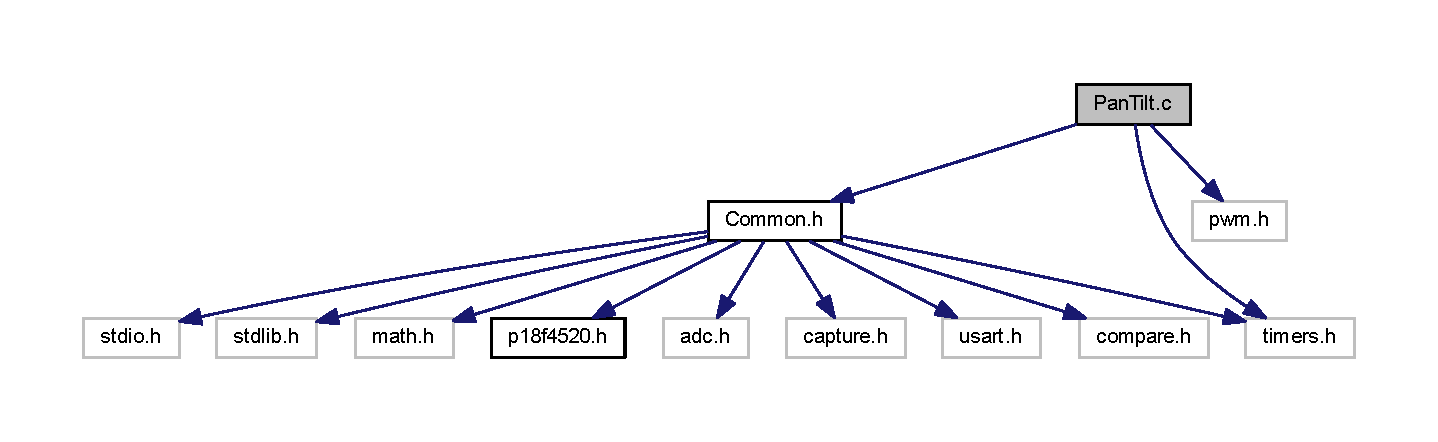
\includegraphics[width=350pt]{_pan_tilt_8c__incl}
\end{center}
\end{figure}
\subsection*{Data Structures}
\begin{DoxyCompactItemize}
\item 
struct \hyperlink{struct_delay}{Delay}
\end{DoxyCompactItemize}
\subsection*{Macros}
\begin{DoxyCompactItemize}
\item 
\#define \hyperlink{_pan_tilt_8c_a5875ffe458eee073cec6bd62e08679c9}{A\+Z\+\_\+\+P\+W\+M\+\_\+\+P\+I\+N}~\hyperlink{p18f4520_8h_a7ea5e081e0d3ea33ca014db57540107d}{P\+O\+R\+T\+Cbits.\+R\+C0}
\item 
\#define \hyperlink{_pan_tilt_8c_aeccd74b3aafd22092066790005320b98}{I\+N\+\_\+\+P\+W\+M\+\_\+\+P\+I\+N}~\hyperlink{p18f4520_8h_acbac2bc4f50222ec7e8549d800993842}{P\+O\+R\+T\+Cbits.\+R\+C1}
\item 
\#define \hyperlink{_pan_tilt_8c_a8fae060499b6b4a82b757f7b7f082f36}{D\+U\+T\+Y\+\_\+\+C\+Y\+C\+L\+E\+\_\+\+T\+I\+M\+E}~2500
\item 
\#define \hyperlink{_pan_tilt_8c_aacaca0988244bd3a888ca5befa89f44b}{P\+W\+M\+\_\+\+P\+E\+R\+I\+O\+D}~50000
\item 
\#define \hyperlink{_pan_tilt_8c_ac829b6acf6662103690f1bca3c422f34}{P\+W\+M\+\_\+\+H\+A\+L\+F\+\_\+\+P\+E\+R\+I\+O\+D}~25000
\item 
\#define \hyperlink{_pan_tilt_8c_a32ba76cc676dc9b248bce3b722e811e5}{L\+A\+T\+E\+N\+C\+Y}~340
\item 
\#define \hyperlink{_pan_tilt_8c_afed42813fde734ec03d642316c880a8f}{S\+E\+R\+V\+O\+\_\+\+I\+N\+I\+T}()~\hyperlink{p18f4520_8h_a7ea5e081e0d3ea33ca014db57540107d}{T\+R\+I\+S\+Cbits.\+R\+C0} = 0; \hyperlink{p18f4520_8h_acbac2bc4f50222ec7e8549d800993842}{T\+R\+I\+S\+Cbits.\+R\+C1} = 0; \hyperlink{p18f4520_8h_a7ea5e081e0d3ea33ca014db57540107d}{P\+O\+R\+T\+Cbits.\+R\+C0} = 0; \hyperlink{p18f4520_8h_acbac2bc4f50222ec7e8549d800993842}{P\+O\+R\+T\+Cbits.\+R\+C1} = 0
\end{DoxyCompactItemize}
\subsection*{Functions}
\begin{DoxyCompactItemize}
\item 
void \hyperlink{_pan_tilt_8c_ab7b8c8f7bf051b4f8e3b151f7b567127}{configure\+Base} (void)
\item 
void \hyperlink{_pan_tilt_8c_a032fbfc434ca24d27d89b6d768455a42}{move} (\hyperlink{struct_direction}{Direction} destination)
\item 
void \hyperlink{_pan_tilt_8c_af8e57fbe1513bb48274f4f0f46717fa1}{increment} (\hyperlink{struct_direction}{Direction} difference)
\item 
void \hyperlink{_pan_tilt_8c_a5350e3f473fb25899612d382c1baa642}{increment\+Fine} (\hyperlink{struct_direction}{Direction} difference)
\item 
\hyperlink{struct_direction}{Direction} \hyperlink{_pan_tilt_8c_ad1d9638bad5a5021969d19769e70c775}{get\+Dir} (void)
\item 
char \hyperlink{_pan_tilt_8c_ae8f9ea5919de15d1b5614be2e5e65be3}{get\+Max\+Azimuth\+Angle} (void)
\item 
char \hyperlink{_pan_tilt_8c_af45dd498eebe7f5ba7b228c15e7221c1}{get\+Min\+Azimuth\+Angle} (void)
\item 
char \hyperlink{_pan_tilt_8c_a4278dbef7fe9034a7a54d02bcbb16de9}{get\+Max\+Elevation\+Angle} (void)
\item 
char \hyperlink{_pan_tilt_8c_af7fafa63e9c645a80f28aca253bba5cc}{get\+Min\+Elevation\+Angle} (void)
\item 
void \hyperlink{_pan_tilt_8c_a1f5e600a2655aeb9dd24b8325a777931}{set\+Max\+Azimuth\+Angle} (char p\+\_\+angle)
\item 
void \hyperlink{_pan_tilt_8c_a157ea38d68fcd31082dc2eaba2944ef3}{set\+Min\+Azimuth\+Angle} (char p\+\_\+angle)
\item 
void \hyperlink{_pan_tilt_8c_aa956697480994a26cb592b2cfcf3436c}{set\+Max\+Elevation\+Angle} (char p\+\_\+angle)
\item 
void \hyperlink{_pan_tilt_8c_a001917f3c38b200d142ab6932991e001}{set\+Min\+Elevation\+Angle} (char p\+\_\+angle)
\item 
void \hyperlink{_pan_tilt_8c_a60e08860a1b4ca9efdc2dd43983731d5}{calibrate\+Pan\+Tilt} (\hyperlink{struct_direction}{Direction} reference)
\item 
\hyperlink{struct_direction}{Direction} \hyperlink{_pan_tilt_8c_a251ee95d75c68e21c4bb933ac99e5108}{raw\+Dir} (void)
\item 
void \hyperlink{_pan_tilt_8c_a7f353056fb02f0d95fd997198f5b186f}{pan\+Tilt\+I\+S\+R} (void)
\item 
char \hyperlink{_pan_tilt_8c_a3362a0aacdd7037d0329989d353c60b7}{updated} (void)
\end{DoxyCompactItemize}


\subsection{Macro Definition Documentation}
\hypertarget{_pan_tilt_8c_a5875ffe458eee073cec6bd62e08679c9}{\index{Pan\+Tilt.\+c@{Pan\+Tilt.\+c}!A\+Z\+\_\+\+P\+W\+M\+\_\+\+P\+I\+N@{A\+Z\+\_\+\+P\+W\+M\+\_\+\+P\+I\+N}}
\index{A\+Z\+\_\+\+P\+W\+M\+\_\+\+P\+I\+N@{A\+Z\+\_\+\+P\+W\+M\+\_\+\+P\+I\+N}!Pan\+Tilt.\+c@{Pan\+Tilt.\+c}}
\subsubsection[{A\+Z\+\_\+\+P\+W\+M\+\_\+\+P\+I\+N}]{\setlength{\rightskip}{0pt plus 5cm}\#define A\+Z\+\_\+\+P\+W\+M\+\_\+\+P\+I\+N~{\bf P\+O\+R\+T\+Cbits.\+R\+C0}}}\label{_pan_tilt_8c_a5875ffe458eee073cec6bd62e08679c9}


Definition at line 56 of file Pan\+Tilt.\+c.

\hypertarget{_pan_tilt_8c_a8fae060499b6b4a82b757f7b7f082f36}{\index{Pan\+Tilt.\+c@{Pan\+Tilt.\+c}!D\+U\+T\+Y\+\_\+\+C\+Y\+C\+L\+E\+\_\+\+T\+I\+M\+E@{D\+U\+T\+Y\+\_\+\+C\+Y\+C\+L\+E\+\_\+\+T\+I\+M\+E}}
\index{D\+U\+T\+Y\+\_\+\+C\+Y\+C\+L\+E\+\_\+\+T\+I\+M\+E@{D\+U\+T\+Y\+\_\+\+C\+Y\+C\+L\+E\+\_\+\+T\+I\+M\+E}!Pan\+Tilt.\+c@{Pan\+Tilt.\+c}}
\subsubsection[{D\+U\+T\+Y\+\_\+\+C\+Y\+C\+L\+E\+\_\+\+T\+I\+M\+E}]{\setlength{\rightskip}{0pt plus 5cm}\#define D\+U\+T\+Y\+\_\+\+C\+Y\+C\+L\+E\+\_\+\+T\+I\+M\+E~2500}}\label{_pan_tilt_8c_a8fae060499b6b4a82b757f7b7f082f36}


Definition at line 60 of file Pan\+Tilt.\+c.

\hypertarget{_pan_tilt_8c_aeccd74b3aafd22092066790005320b98}{\index{Pan\+Tilt.\+c@{Pan\+Tilt.\+c}!I\+N\+\_\+\+P\+W\+M\+\_\+\+P\+I\+N@{I\+N\+\_\+\+P\+W\+M\+\_\+\+P\+I\+N}}
\index{I\+N\+\_\+\+P\+W\+M\+\_\+\+P\+I\+N@{I\+N\+\_\+\+P\+W\+M\+\_\+\+P\+I\+N}!Pan\+Tilt.\+c@{Pan\+Tilt.\+c}}
\subsubsection[{I\+N\+\_\+\+P\+W\+M\+\_\+\+P\+I\+N}]{\setlength{\rightskip}{0pt plus 5cm}\#define I\+N\+\_\+\+P\+W\+M\+\_\+\+P\+I\+N~{\bf P\+O\+R\+T\+Cbits.\+R\+C1}}}\label{_pan_tilt_8c_aeccd74b3aafd22092066790005320b98}


Definition at line 57 of file Pan\+Tilt.\+c.

\hypertarget{_pan_tilt_8c_a32ba76cc676dc9b248bce3b722e811e5}{\index{Pan\+Tilt.\+c@{Pan\+Tilt.\+c}!L\+A\+T\+E\+N\+C\+Y@{L\+A\+T\+E\+N\+C\+Y}}
\index{L\+A\+T\+E\+N\+C\+Y@{L\+A\+T\+E\+N\+C\+Y}!Pan\+Tilt.\+c@{Pan\+Tilt.\+c}}
\subsubsection[{L\+A\+T\+E\+N\+C\+Y}]{\setlength{\rightskip}{0pt plus 5cm}\#define L\+A\+T\+E\+N\+C\+Y~340}}\label{_pan_tilt_8c_a32ba76cc676dc9b248bce3b722e811e5}


Definition at line 70 of file Pan\+Tilt.\+c.

\hypertarget{_pan_tilt_8c_ac829b6acf6662103690f1bca3c422f34}{\index{Pan\+Tilt.\+c@{Pan\+Tilt.\+c}!P\+W\+M\+\_\+\+H\+A\+L\+F\+\_\+\+P\+E\+R\+I\+O\+D@{P\+W\+M\+\_\+\+H\+A\+L\+F\+\_\+\+P\+E\+R\+I\+O\+D}}
\index{P\+W\+M\+\_\+\+H\+A\+L\+F\+\_\+\+P\+E\+R\+I\+O\+D@{P\+W\+M\+\_\+\+H\+A\+L\+F\+\_\+\+P\+E\+R\+I\+O\+D}!Pan\+Tilt.\+c@{Pan\+Tilt.\+c}}
\subsubsection[{P\+W\+M\+\_\+\+H\+A\+L\+F\+\_\+\+P\+E\+R\+I\+O\+D}]{\setlength{\rightskip}{0pt plus 5cm}\#define P\+W\+M\+\_\+\+H\+A\+L\+F\+\_\+\+P\+E\+R\+I\+O\+D~25000}}\label{_pan_tilt_8c_ac829b6acf6662103690f1bca3c422f34}


Definition at line 62 of file Pan\+Tilt.\+c.

\hypertarget{_pan_tilt_8c_aacaca0988244bd3a888ca5befa89f44b}{\index{Pan\+Tilt.\+c@{Pan\+Tilt.\+c}!P\+W\+M\+\_\+\+P\+E\+R\+I\+O\+D@{P\+W\+M\+\_\+\+P\+E\+R\+I\+O\+D}}
\index{P\+W\+M\+\_\+\+P\+E\+R\+I\+O\+D@{P\+W\+M\+\_\+\+P\+E\+R\+I\+O\+D}!Pan\+Tilt.\+c@{Pan\+Tilt.\+c}}
\subsubsection[{P\+W\+M\+\_\+\+P\+E\+R\+I\+O\+D}]{\setlength{\rightskip}{0pt plus 5cm}\#define P\+W\+M\+\_\+\+P\+E\+R\+I\+O\+D~50000}}\label{_pan_tilt_8c_aacaca0988244bd3a888ca5befa89f44b}


Definition at line 61 of file Pan\+Tilt.\+c.

\hypertarget{_pan_tilt_8c_afed42813fde734ec03d642316c880a8f}{\index{Pan\+Tilt.\+c@{Pan\+Tilt.\+c}!S\+E\+R\+V\+O\+\_\+\+I\+N\+I\+T@{S\+E\+R\+V\+O\+\_\+\+I\+N\+I\+T}}
\index{S\+E\+R\+V\+O\+\_\+\+I\+N\+I\+T@{S\+E\+R\+V\+O\+\_\+\+I\+N\+I\+T}!Pan\+Tilt.\+c@{Pan\+Tilt.\+c}}
\subsubsection[{S\+E\+R\+V\+O\+\_\+\+I\+N\+I\+T}]{\setlength{\rightskip}{0pt plus 5cm}\#define S\+E\+R\+V\+O\+\_\+\+I\+N\+I\+T(
\begin{DoxyParamCaption}
{}
\end{DoxyParamCaption}
)~{\bf T\+R\+I\+S\+Cbits.\+R\+C0} = 0; {\bf T\+R\+I\+S\+Cbits.\+R\+C1} = 0; {\bf P\+O\+R\+T\+Cbits.\+R\+C0} = 0; {\bf P\+O\+R\+T\+Cbits.\+R\+C1} = 0}}\label{_pan_tilt_8c_afed42813fde734ec03d642316c880a8f}


Definition at line 72 of file Pan\+Tilt.\+c.



\subsection{Function Documentation}
\hypertarget{_pan_tilt_8c_a60e08860a1b4ca9efdc2dd43983731d5}{\index{Pan\+Tilt.\+c@{Pan\+Tilt.\+c}!calibrate\+Pan\+Tilt@{calibrate\+Pan\+Tilt}}
\index{calibrate\+Pan\+Tilt@{calibrate\+Pan\+Tilt}!Pan\+Tilt.\+c@{Pan\+Tilt.\+c}}
\subsubsection[{calibrate\+Pan\+Tilt}]{\setlength{\rightskip}{0pt plus 5cm}void calibrate\+Pan\+Tilt (
\begin{DoxyParamCaption}
\item[{{\bf Direction}}]{reference}
\end{DoxyParamCaption}
)}}\label{_pan_tilt_8c_a60e08860a1b4ca9efdc2dd43983731d5}


 Function\+: \hyperlink{_pan_tilt_8c_a60e08860a1b4ca9efdc2dd43983731d5}{calibrate\+Pan\+Tilt(\+Direction reference)}

Include\+: \hyperlink{_pan_tilt_8h}{Pan\+Tilt.\+h}

Description\+: Calibrates the pan tile mechanism so that any future reference to move to the reference value specified in the function call will move the pan tilt back to the current position.

Arguments\+: reference -\/ A struct containing the azimuth and inclinaion you wish to define as this position.

Returns\+: None 

Definition at line 364 of file Pan\+Tilt.\+c.

\hypertarget{_pan_tilt_8c_ab7b8c8f7bf051b4f8e3b151f7b567127}{\index{Pan\+Tilt.\+c@{Pan\+Tilt.\+c}!configure\+Base@{configure\+Base}}
\index{configure\+Base@{configure\+Base}!Pan\+Tilt.\+c@{Pan\+Tilt.\+c}}
\subsubsection[{configure\+Base}]{\setlength{\rightskip}{0pt plus 5cm}void configure\+Base (
\begin{DoxyParamCaption}
\item[{void}]{}
\end{DoxyParamCaption}
)}}\label{_pan_tilt_8c_ab7b8c8f7bf051b4f8e3b151f7b567127}


 Function\+: \hyperlink{_pan_tilt_8c_ab7b8c8f7bf051b4f8e3b151f7b567127}{configure\+Base(void)}

Include\+: \hyperlink{_pan_tilt_8h}{Pan\+Tilt.\+h}

Description\+: Configures the Pan Tilt mechanism for operation

Arguments\+: None

Returns\+: None 

Definition at line 105 of file Pan\+Tilt.\+c.



Here is the caller graph for this function\+:\nopagebreak
\begin{figure}[H]
\begin{center}
\leavevmode
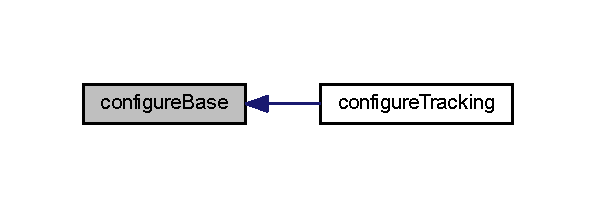
\includegraphics[width=286pt]{_pan_tilt_8c_ab7b8c8f7bf051b4f8e3b151f7b567127_icgraph}
\end{center}
\end{figure}


\hypertarget{_pan_tilt_8c_ad1d9638bad5a5021969d19769e70c775}{\index{Pan\+Tilt.\+c@{Pan\+Tilt.\+c}!get\+Dir@{get\+Dir}}
\index{get\+Dir@{get\+Dir}!Pan\+Tilt.\+c@{Pan\+Tilt.\+c}}
\subsubsection[{get\+Dir}]{\setlength{\rightskip}{0pt plus 5cm}{\bf Direction} get\+Dir (
\begin{DoxyParamCaption}
\item[{void}]{}
\end{DoxyParamCaption}
)}}\label{_pan_tilt_8c_ad1d9638bad5a5021969d19769e70c775}


 Function\+: \hyperlink{_pan_tilt_8c_ad1d9638bad5a5021969d19769e70c775}{get\+Dir(void)}

Include\+: \hyperlink{_pan_tilt_8h}{Pan\+Tilt.\+h}

Description\+: returns the current position of the pan tilt mechanism

Arguments\+: None

Returns\+: A struct containing the azimuth and inclination 

Definition at line 219 of file Pan\+Tilt.\+c.



Here is the caller graph for this function\+:\nopagebreak
\begin{figure}[H]
\begin{center}
\leavevmode
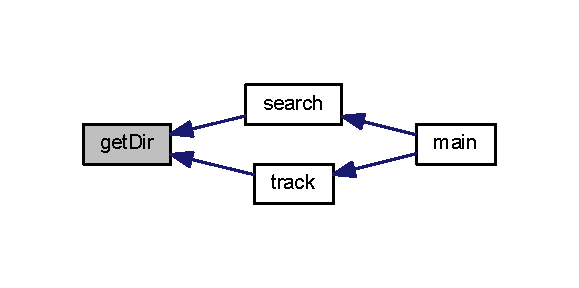
\includegraphics[width=278pt]{_pan_tilt_8c_ad1d9638bad5a5021969d19769e70c775_icgraph}
\end{center}
\end{figure}


\hypertarget{_pan_tilt_8c_ae8f9ea5919de15d1b5614be2e5e65be3}{\index{Pan\+Tilt.\+c@{Pan\+Tilt.\+c}!get\+Max\+Azimuth\+Angle@{get\+Max\+Azimuth\+Angle}}
\index{get\+Max\+Azimuth\+Angle@{get\+Max\+Azimuth\+Angle}!Pan\+Tilt.\+c@{Pan\+Tilt.\+c}}
\subsubsection[{get\+Max\+Azimuth\+Angle}]{\setlength{\rightskip}{0pt plus 5cm}char get\+Max\+Azimuth\+Angle (
\begin{DoxyParamCaption}
\item[{void}]{}
\end{DoxyParamCaption}
)}}\label{_pan_tilt_8c_ae8f9ea5919de15d1b5614be2e5e65be3}


 Function\+: \hyperlink{_pan_tilt_8c_ae8f9ea5919de15d1b5614be2e5e65be3}{get\+Max\+Azimuth\+Angle(void)}

Include\+: \hyperlink{_pan_tilt_8h}{Pan\+Tilt.\+h}

Description\+: returns the maximum angle of the azimuth servo

Arguments\+: None

Returns\+: A char with the maximum azimuth angle. 

Definition at line 235 of file Pan\+Tilt.\+c.

\hypertarget{_pan_tilt_8c_a4278dbef7fe9034a7a54d02bcbb16de9}{\index{Pan\+Tilt.\+c@{Pan\+Tilt.\+c}!get\+Max\+Elevation\+Angle@{get\+Max\+Elevation\+Angle}}
\index{get\+Max\+Elevation\+Angle@{get\+Max\+Elevation\+Angle}!Pan\+Tilt.\+c@{Pan\+Tilt.\+c}}
\subsubsection[{get\+Max\+Elevation\+Angle}]{\setlength{\rightskip}{0pt plus 5cm}char get\+Max\+Elevation\+Angle (
\begin{DoxyParamCaption}
\item[{void}]{}
\end{DoxyParamCaption}
)}}\label{_pan_tilt_8c_a4278dbef7fe9034a7a54d02bcbb16de9}


 Function\+: \hyperlink{_pan_tilt_8c_a4278dbef7fe9034a7a54d02bcbb16de9}{get\+Max\+Elevation\+Angle(void)}

Include\+: \hyperlink{_pan_tilt_8h}{Pan\+Tilt.\+h}

Description\+: returns the maximum angle of the elevation servo

Arguments\+: None

Returns\+: A char with the maximum elevation angle. 

Definition at line 267 of file Pan\+Tilt.\+c.

\hypertarget{_pan_tilt_8c_af45dd498eebe7f5ba7b228c15e7221c1}{\index{Pan\+Tilt.\+c@{Pan\+Tilt.\+c}!get\+Min\+Azimuth\+Angle@{get\+Min\+Azimuth\+Angle}}
\index{get\+Min\+Azimuth\+Angle@{get\+Min\+Azimuth\+Angle}!Pan\+Tilt.\+c@{Pan\+Tilt.\+c}}
\subsubsection[{get\+Min\+Azimuth\+Angle}]{\setlength{\rightskip}{0pt plus 5cm}char get\+Min\+Azimuth\+Angle (
\begin{DoxyParamCaption}
\item[{void}]{}
\end{DoxyParamCaption}
)}}\label{_pan_tilt_8c_af45dd498eebe7f5ba7b228c15e7221c1}


 Function\+: \hyperlink{_pan_tilt_8c_af45dd498eebe7f5ba7b228c15e7221c1}{get\+Min\+Azimuth\+Angle(void)}

Include\+: \hyperlink{_pan_tilt_8h}{Pan\+Tilt.\+h}

Description\+: returns the minimum angle of the azimuth servo

Arguments\+: None

Returns\+: A char with the minimum azimuth angle. 

Definition at line 251 of file Pan\+Tilt.\+c.

\hypertarget{_pan_tilt_8c_af7fafa63e9c645a80f28aca253bba5cc}{\index{Pan\+Tilt.\+c@{Pan\+Tilt.\+c}!get\+Min\+Elevation\+Angle@{get\+Min\+Elevation\+Angle}}
\index{get\+Min\+Elevation\+Angle@{get\+Min\+Elevation\+Angle}!Pan\+Tilt.\+c@{Pan\+Tilt.\+c}}
\subsubsection[{get\+Min\+Elevation\+Angle}]{\setlength{\rightskip}{0pt plus 5cm}char get\+Min\+Elevation\+Angle (
\begin{DoxyParamCaption}
\item[{void}]{}
\end{DoxyParamCaption}
)}}\label{_pan_tilt_8c_af7fafa63e9c645a80f28aca253bba5cc}


 Function\+: \hyperlink{_pan_tilt_8c_af7fafa63e9c645a80f28aca253bba5cc}{get\+Min\+Elevation\+Angle(void)}

Include\+: \hyperlink{_pan_tilt_8h}{Pan\+Tilt.\+h}

Description\+: returns the minimum angle of the elevation servo

Arguments\+: None

Returns\+: A char with the minimum elevation angle. 

Definition at line 283 of file Pan\+Tilt.\+c.

\hypertarget{_pan_tilt_8c_af8e57fbe1513bb48274f4f0f46717fa1}{\index{Pan\+Tilt.\+c@{Pan\+Tilt.\+c}!increment@{increment}}
\index{increment@{increment}!Pan\+Tilt.\+c@{Pan\+Tilt.\+c}}
\subsubsection[{increment}]{\setlength{\rightskip}{0pt plus 5cm}void increment (
\begin{DoxyParamCaption}
\item[{{\bf Direction}}]{difference}
\end{DoxyParamCaption}
)}}\label{_pan_tilt_8c_af8e57fbe1513bb48274f4f0f46717fa1}


 Function\+: \hyperlink{_pan_tilt_8c_af8e57fbe1513bb48274f4f0f46717fa1}{increment(\+Direction difference)}

Include\+: \hyperlink{_pan_tilt_8h}{Pan\+Tilt.\+h}

Description\+: Moves the pan tilt actuator to the specified destination

Arguments\+: destionation -\/ A struct containing the desired azimuth and inclination

Returns\+: None 

Definition at line 170 of file Pan\+Tilt.\+c.



Here is the call graph for this function\+:\nopagebreak
\begin{figure}[H]
\begin{center}
\leavevmode
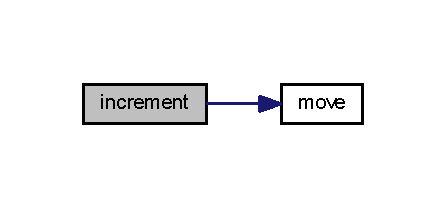
\includegraphics[width=214pt]{_pan_tilt_8c_af8e57fbe1513bb48274f4f0f46717fa1_cgraph}
\end{center}
\end{figure}




Here is the caller graph for this function\+:\nopagebreak
\begin{figure}[H]
\begin{center}
\leavevmode
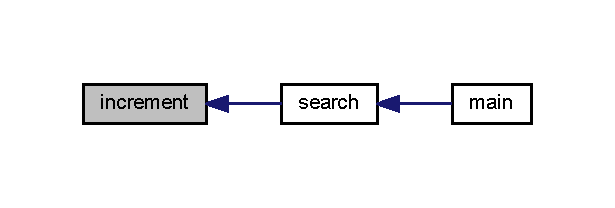
\includegraphics[width=295pt]{_pan_tilt_8c_af8e57fbe1513bb48274f4f0f46717fa1_icgraph}
\end{center}
\end{figure}


\hypertarget{_pan_tilt_8c_a5350e3f473fb25899612d382c1baa642}{\index{Pan\+Tilt.\+c@{Pan\+Tilt.\+c}!increment\+Fine@{increment\+Fine}}
\index{increment\+Fine@{increment\+Fine}!Pan\+Tilt.\+c@{Pan\+Tilt.\+c}}
\subsubsection[{increment\+Fine}]{\setlength{\rightskip}{0pt plus 5cm}void increment\+Fine (
\begin{DoxyParamCaption}
\item[{{\bf Direction}}]{difference}
\end{DoxyParamCaption}
)}}\label{_pan_tilt_8c_a5350e3f473fb25899612d382c1baa642}


 Function\+: \hyperlink{_pan_tilt_8c_a5350e3f473fb25899612d382c1baa642}{increment\+Fine(\+Direction difference)}

Include\+: \hyperlink{_pan_tilt_8h}{Pan\+Tilt.\+h}

Description\+: Moves the pan tilt actuator to the specified (Relative) destination

Arguments\+: destionation -\/ A struct containing the desired azimuth and inclination

Returns\+: None 

Definition at line 189 of file Pan\+Tilt.\+c.

\hypertarget{_pan_tilt_8c_a032fbfc434ca24d27d89b6d768455a42}{\index{Pan\+Tilt.\+c@{Pan\+Tilt.\+c}!move@{move}}
\index{move@{move}!Pan\+Tilt.\+c@{Pan\+Tilt.\+c}}
\subsubsection[{move}]{\setlength{\rightskip}{0pt plus 5cm}void move (
\begin{DoxyParamCaption}
\item[{{\bf Direction}}]{destination}
\end{DoxyParamCaption}
)}}\label{_pan_tilt_8c_a032fbfc434ca24d27d89b6d768455a42}


 Function\+: \hyperlink{_pan_tilt_8c_a032fbfc434ca24d27d89b6d768455a42}{move(\+Direction destination)}

Include\+: \hyperlink{_pan_tilt_8h}{Pan\+Tilt.\+h}

Description\+: Moves the pan tilt actuator to the specified destination

Arguments\+: destionation -\/ A struct containing the desired azimuth and inclination

Returns\+: None 

Definition at line 148 of file Pan\+Tilt.\+c.



Here is the caller graph for this function\+:\nopagebreak
\begin{figure}[H]
\begin{center}
\leavevmode
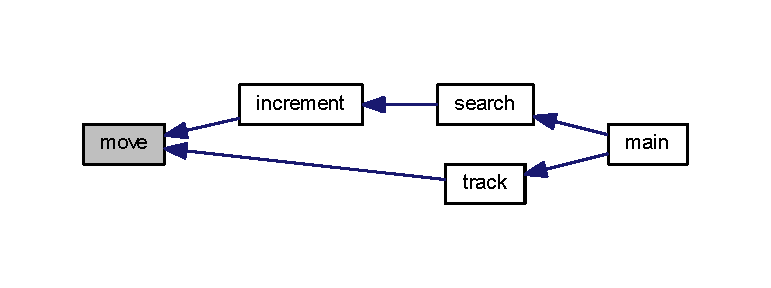
\includegraphics[width=350pt]{_pan_tilt_8c_a032fbfc434ca24d27d89b6d768455a42_icgraph}
\end{center}
\end{figure}


\hypertarget{_pan_tilt_8c_a7f353056fb02f0d95fd997198f5b186f}{\index{Pan\+Tilt.\+c@{Pan\+Tilt.\+c}!pan\+Tilt\+I\+S\+R@{pan\+Tilt\+I\+S\+R}}
\index{pan\+Tilt\+I\+S\+R@{pan\+Tilt\+I\+S\+R}!Pan\+Tilt.\+c@{Pan\+Tilt.\+c}}
\subsubsection[{pan\+Tilt\+I\+S\+R}]{\setlength{\rightskip}{0pt plus 5cm}void pan\+Tilt\+I\+S\+R (
\begin{DoxyParamCaption}
\item[{void}]{}
\end{DoxyParamCaption}
)}}\label{_pan_tilt_8c_a7f353056fb02f0d95fd997198f5b186f}


 Function\+: \hyperlink{_pan_tilt_8c_a7f353056fb02f0d95fd997198f5b186f}{pan\+Tilt\+I\+S\+R(void)}

Include\+: \hyperlink{_pan_tilt_8h}{Pan\+Tilt.\+h}

Description\+: Acts as the I\+S\+R for the Pan\+Tilt module

Arguments\+: None

Returns\+: None 

Definition at line 396 of file Pan\+Tilt.\+c.



Here is the caller graph for this function\+:\nopagebreak
\begin{figure}[H]
\begin{center}
\leavevmode
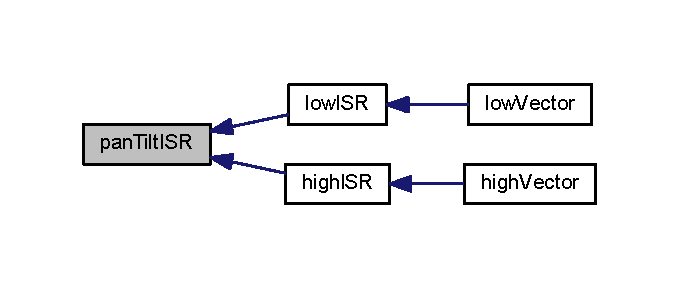
\includegraphics[width=326pt]{_pan_tilt_8c_a7f353056fb02f0d95fd997198f5b186f_icgraph}
\end{center}
\end{figure}


\hypertarget{_pan_tilt_8c_a251ee95d75c68e21c4bb933ac99e5108}{\index{Pan\+Tilt.\+c@{Pan\+Tilt.\+c}!raw\+Dir@{raw\+Dir}}
\index{raw\+Dir@{raw\+Dir}!Pan\+Tilt.\+c@{Pan\+Tilt.\+c}}
\subsubsection[{raw\+Dir}]{\setlength{\rightskip}{0pt plus 5cm}{\bf Direction} raw\+Dir (
\begin{DoxyParamCaption}
\item[{void}]{}
\end{DoxyParamCaption}
)}}\label{_pan_tilt_8c_a251ee95d75c68e21c4bb933ac99e5108}


 Function\+: \hyperlink{_pan_tilt_8c_a251ee95d75c68e21c4bb933ac99e5108}{raw\+Dir(void)}

Include\+: \hyperlink{_pan_tilt_8h}{Pan\+Tilt.\+h}

Description\+: returns the current Pan\+Tile position without calibrating

Arguments\+: None

Returns\+: The position of the pan tilt without any calibration 

Definition at line 380 of file Pan\+Tilt.\+c.

\hypertarget{_pan_tilt_8c_a1f5e600a2655aeb9dd24b8325a777931}{\index{Pan\+Tilt.\+c@{Pan\+Tilt.\+c}!set\+Max\+Azimuth\+Angle@{set\+Max\+Azimuth\+Angle}}
\index{set\+Max\+Azimuth\+Angle@{set\+Max\+Azimuth\+Angle}!Pan\+Tilt.\+c@{Pan\+Tilt.\+c}}
\subsubsection[{set\+Max\+Azimuth\+Angle}]{\setlength{\rightskip}{0pt plus 5cm}void set\+Max\+Azimuth\+Angle (
\begin{DoxyParamCaption}
\item[{char}]{p\+\_\+angle}
\end{DoxyParamCaption}
)}}\label{_pan_tilt_8c_a1f5e600a2655aeb9dd24b8325a777931}


 Function\+: set\+Max\+Azimuth\+Angle(void)

Include\+: \hyperlink{_pan_tilt_8h}{Pan\+Tilt.\+h}

Description\+: sets the maximum angle of the azimuth servo

Arguments\+: The maximum angle (as char) to set for the azimuth servo

Returns\+: None. 

Definition at line 299 of file Pan\+Tilt.\+c.

\hypertarget{_pan_tilt_8c_aa956697480994a26cb592b2cfcf3436c}{\index{Pan\+Tilt.\+c@{Pan\+Tilt.\+c}!set\+Max\+Elevation\+Angle@{set\+Max\+Elevation\+Angle}}
\index{set\+Max\+Elevation\+Angle@{set\+Max\+Elevation\+Angle}!Pan\+Tilt.\+c@{Pan\+Tilt.\+c}}
\subsubsection[{set\+Max\+Elevation\+Angle}]{\setlength{\rightskip}{0pt plus 5cm}void set\+Max\+Elevation\+Angle (
\begin{DoxyParamCaption}
\item[{char}]{p\+\_\+angle}
\end{DoxyParamCaption}
)}}\label{_pan_tilt_8c_aa956697480994a26cb592b2cfcf3436c}


 Function\+: set\+Max\+Elevation\+Angle(void)

Include\+: \hyperlink{_pan_tilt_8h}{Pan\+Tilt.\+h}

Description\+: sets the maximum angle of the elevation servo

Arguments\+: The maximum angle (as char) to set for the elevation servo

Returns\+: None. 

Definition at line 329 of file Pan\+Tilt.\+c.

\hypertarget{_pan_tilt_8c_a157ea38d68fcd31082dc2eaba2944ef3}{\index{Pan\+Tilt.\+c@{Pan\+Tilt.\+c}!set\+Min\+Azimuth\+Angle@{set\+Min\+Azimuth\+Angle}}
\index{set\+Min\+Azimuth\+Angle@{set\+Min\+Azimuth\+Angle}!Pan\+Tilt.\+c@{Pan\+Tilt.\+c}}
\subsubsection[{set\+Min\+Azimuth\+Angle}]{\setlength{\rightskip}{0pt plus 5cm}void set\+Min\+Azimuth\+Angle (
\begin{DoxyParamCaption}
\item[{char}]{p\+\_\+angle}
\end{DoxyParamCaption}
)}}\label{_pan_tilt_8c_a157ea38d68fcd31082dc2eaba2944ef3}


 Function\+: set\+Min\+Azimuth\+Angle(void)

Include\+: \hyperlink{_pan_tilt_8h}{Pan\+Tilt.\+h}

Description\+: sets the minimum angle of the azimuth servo

Arguments\+: The minimum angle (as char) to set for the azimuth servo

Returns\+: None. 

Definition at line 314 of file Pan\+Tilt.\+c.

\hypertarget{_pan_tilt_8c_a001917f3c38b200d142ab6932991e001}{\index{Pan\+Tilt.\+c@{Pan\+Tilt.\+c}!set\+Min\+Elevation\+Angle@{set\+Min\+Elevation\+Angle}}
\index{set\+Min\+Elevation\+Angle@{set\+Min\+Elevation\+Angle}!Pan\+Tilt.\+c@{Pan\+Tilt.\+c}}
\subsubsection[{set\+Min\+Elevation\+Angle}]{\setlength{\rightskip}{0pt plus 5cm}void set\+Min\+Elevation\+Angle (
\begin{DoxyParamCaption}
\item[{char}]{p\+\_\+angle}
\end{DoxyParamCaption}
)}}\label{_pan_tilt_8c_a001917f3c38b200d142ab6932991e001}


 Function\+: set\+Min\+Elevation\+Angle(void)

Include\+: \hyperlink{_pan_tilt_8h}{Pan\+Tilt.\+h}

Description\+: sets the minimum angle of the elevation servo

Arguments\+: The minimum angle (as char) to set for the elevation servo

Returns\+: None. 

Definition at line 345 of file Pan\+Tilt.\+c.

\hypertarget{_pan_tilt_8c_a3362a0aacdd7037d0329989d353c60b7}{\index{Pan\+Tilt.\+c@{Pan\+Tilt.\+c}!updated@{updated}}
\index{updated@{updated}!Pan\+Tilt.\+c@{Pan\+Tilt.\+c}}
\subsubsection[{updated}]{\setlength{\rightskip}{0pt plus 5cm}char updated (
\begin{DoxyParamCaption}
\item[{void}]{}
\end{DoxyParamCaption}
)}}\label{_pan_tilt_8c_a3362a0aacdd7037d0329989d353c60b7}


 Function\+: \hyperlink{_pan_tilt_8c_a3362a0aacdd7037d0329989d353c60b7}{updated(void)}

Include\+: \hyperlink{_pan_tilt_8h}{Pan\+Tilt.\+h}

Description\+: returns true if the last move or increment or increment\+Fine function has taken effect. The new direction is only loaded in at the end of the P\+D\+M, so it could take up to 0.\+02 seconds for the change to take effect.

Arguments\+: delay -\/ a pointer to the delay variable

Returns\+: None 

Definition at line 532 of file Pan\+Tilt.\+c.


\hypertarget{_pan_tilt_8h}{\section{Pan\+Tilt.\+h File Reference}
\label{_pan_tilt_8h}\index{Pan\+Tilt.\+h@{Pan\+Tilt.\+h}}
}
This graph shows which files directly or indirectly include this file\+:\nopagebreak
\begin{figure}[H]
\begin{center}
\leavevmode
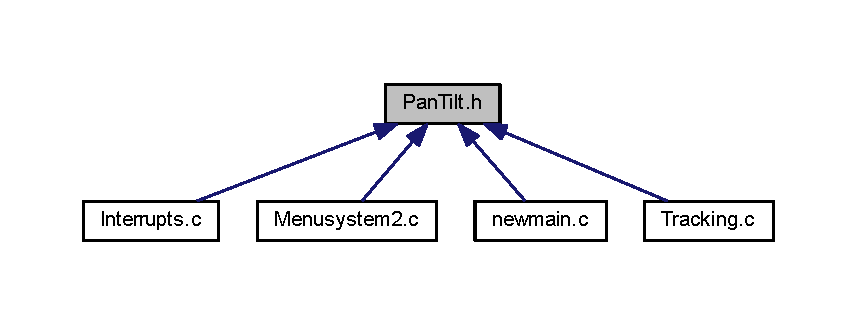
\includegraphics[width=350pt]{_pan_tilt_8h__dep__incl}
\end{center}
\end{figure}
\subsection*{Macros}
\begin{DoxyCompactItemize}
\item 
\#define \hyperlink{_pan_tilt_8h_a9f6dec47561ba32094f46e58db44f964}{P\+A\+N\+\_\+\+T\+I\+L\+T\+\_\+\+I\+S\+R}~\hyperlink{_common_8h_aee2ef60613898be37c57266698616e33}{C\+C\+P2\+\_\+\+I\+N\+T}
\item 
\#define \hyperlink{_pan_tilt_8h_a12311b605a58b1d9a311dbb71a160045}{P\+A\+N\+T\+I\+L\+T\+\_\+\+H}
\end{DoxyCompactItemize}
\subsection*{Functions}
\begin{DoxyCompactItemize}
\item 
void \hyperlink{_pan_tilt_8h_ab7b8c8f7bf051b4f8e3b151f7b567127}{configure\+Base} (void)
\item 
void \hyperlink{_pan_tilt_8h_a032fbfc434ca24d27d89b6d768455a42}{move} (\hyperlink{struct_direction}{Direction} destination)
\item 
void \hyperlink{_pan_tilt_8h_af8e57fbe1513bb48274f4f0f46717fa1}{increment} (\hyperlink{struct_direction}{Direction} difference)
\item 
void \hyperlink{_pan_tilt_8h_a5350e3f473fb25899612d382c1baa642}{increment\+Fine} (\hyperlink{struct_direction}{Direction} difference)
\item 
\hyperlink{struct_direction}{Direction} \hyperlink{_pan_tilt_8h_ad1d9638bad5a5021969d19769e70c775}{get\+Dir} (void)
\item 
void \hyperlink{_pan_tilt_8h_a60e08860a1b4ca9efdc2dd43983731d5}{calibrate\+Pan\+Tilt} (\hyperlink{struct_direction}{Direction} reference)
\item 
\hyperlink{struct_direction}{Direction} \hyperlink{_pan_tilt_8h_a251ee95d75c68e21c4bb933ac99e5108}{raw\+Dir} (void)
\item 
char \hyperlink{_pan_tilt_8h_a3362a0aacdd7037d0329989d353c60b7}{updated} (void)
\item 
void \hyperlink{_pan_tilt_8h_a7f353056fb02f0d95fd997198f5b186f}{pan\+Tilt\+I\+S\+R} (void)
\item 
char \hyperlink{_pan_tilt_8h_ae8f9ea5919de15d1b5614be2e5e65be3}{get\+Max\+Azimuth\+Angle} (void)
\item 
char \hyperlink{_pan_tilt_8h_af45dd498eebe7f5ba7b228c15e7221c1}{get\+Min\+Azimuth\+Angle} (void)
\item 
char \hyperlink{_pan_tilt_8h_a4278dbef7fe9034a7a54d02bcbb16de9}{get\+Max\+Elevation\+Angle} (void)
\item 
char \hyperlink{_pan_tilt_8h_af7fafa63e9c645a80f28aca253bba5cc}{get\+Min\+Elevation\+Angle} (void)
\item 
void \hyperlink{_pan_tilt_8h_a1f5e600a2655aeb9dd24b8325a777931}{set\+Max\+Azimuth\+Angle} (char p\+\_\+angle)
\item 
void \hyperlink{_pan_tilt_8h_a157ea38d68fcd31082dc2eaba2944ef3}{set\+Min\+Azimuth\+Angle} (char p\+\_\+angle)
\item 
void \hyperlink{_pan_tilt_8h_aa956697480994a26cb592b2cfcf3436c}{set\+Max\+Elevation\+Angle} (char p\+\_\+angle)
\item 
void \hyperlink{_pan_tilt_8h_a001917f3c38b200d142ab6932991e001}{set\+Min\+Elevation\+Angle} (char p\+\_\+angle)
\end{DoxyCompactItemize}


\subsection{Macro Definition Documentation}
\hypertarget{_pan_tilt_8h_a9f6dec47561ba32094f46e58db44f964}{\index{Pan\+Tilt.\+h@{Pan\+Tilt.\+h}!P\+A\+N\+\_\+\+T\+I\+L\+T\+\_\+\+I\+S\+R@{P\+A\+N\+\_\+\+T\+I\+L\+T\+\_\+\+I\+S\+R}}
\index{P\+A\+N\+\_\+\+T\+I\+L\+T\+\_\+\+I\+S\+R@{P\+A\+N\+\_\+\+T\+I\+L\+T\+\_\+\+I\+S\+R}!Pan\+Tilt.\+h@{Pan\+Tilt.\+h}}
\subsubsection[{P\+A\+N\+\_\+\+T\+I\+L\+T\+\_\+\+I\+S\+R}]{\setlength{\rightskip}{0pt plus 5cm}\#define P\+A\+N\+\_\+\+T\+I\+L\+T\+\_\+\+I\+S\+R~{\bf C\+C\+P2\+\_\+\+I\+N\+T}}}\label{_pan_tilt_8h_a9f6dec47561ba32094f46e58db44f964}


Definition at line 14 of file Pan\+Tilt.\+h.

\hypertarget{_pan_tilt_8h_a12311b605a58b1d9a311dbb71a160045}{\index{Pan\+Tilt.\+h@{Pan\+Tilt.\+h}!P\+A\+N\+T\+I\+L\+T\+\_\+\+H@{P\+A\+N\+T\+I\+L\+T\+\_\+\+H}}
\index{P\+A\+N\+T\+I\+L\+T\+\_\+\+H@{P\+A\+N\+T\+I\+L\+T\+\_\+\+H}!Pan\+Tilt.\+h@{Pan\+Tilt.\+h}}
\subsubsection[{P\+A\+N\+T\+I\+L\+T\+\_\+\+H}]{\setlength{\rightskip}{0pt plus 5cm}\#define P\+A\+N\+T\+I\+L\+T\+\_\+\+H}}\label{_pan_tilt_8h_a12311b605a58b1d9a311dbb71a160045}


Definition at line 37 of file Pan\+Tilt.\+h.



\subsection{Function Documentation}
\hypertarget{_pan_tilt_8h_a60e08860a1b4ca9efdc2dd43983731d5}{\index{Pan\+Tilt.\+h@{Pan\+Tilt.\+h}!calibrate\+Pan\+Tilt@{calibrate\+Pan\+Tilt}}
\index{calibrate\+Pan\+Tilt@{calibrate\+Pan\+Tilt}!Pan\+Tilt.\+h@{Pan\+Tilt.\+h}}
\subsubsection[{calibrate\+Pan\+Tilt}]{\setlength{\rightskip}{0pt plus 5cm}void calibrate\+Pan\+Tilt (
\begin{DoxyParamCaption}
\item[{{\bf Direction}}]{reference}
\end{DoxyParamCaption}
)}}\label{_pan_tilt_8h_a60e08860a1b4ca9efdc2dd43983731d5}


 Function\+: \hyperlink{_pan_tilt_8c_a60e08860a1b4ca9efdc2dd43983731d5}{calibrate\+Pan\+Tilt(\+Direction reference)}

Include\+: \hyperlink{_pan_tilt_8h}{Pan\+Tilt.\+h}

Description\+: Calibrates the pan tile mechanism so that any future reference to move to the reference value specified in the function call will move the pan tilt back to the current position.

Arguments\+: reference -\/ A struct containing the azimuth and inclinaion you wish to define as this position.

Returns\+: None 

Definition at line 364 of file Pan\+Tilt.\+c.

\hypertarget{_pan_tilt_8h_ab7b8c8f7bf051b4f8e3b151f7b567127}{\index{Pan\+Tilt.\+h@{Pan\+Tilt.\+h}!configure\+Base@{configure\+Base}}
\index{configure\+Base@{configure\+Base}!Pan\+Tilt.\+h@{Pan\+Tilt.\+h}}
\subsubsection[{configure\+Base}]{\setlength{\rightskip}{0pt plus 5cm}void configure\+Base (
\begin{DoxyParamCaption}
\item[{void}]{}
\end{DoxyParamCaption}
)}}\label{_pan_tilt_8h_ab7b8c8f7bf051b4f8e3b151f7b567127}


 Function\+: \hyperlink{_pan_tilt_8c_ab7b8c8f7bf051b4f8e3b151f7b567127}{configure\+Base(void)}

Include\+: \hyperlink{_pan_tilt_8h}{Pan\+Tilt.\+h}

Description\+: Configures the Pan Tilt mechanism for operation

Arguments\+: None

Returns\+: None 

Definition at line 105 of file Pan\+Tilt.\+c.



Here is the caller graph for this function\+:\nopagebreak
\begin{figure}[H]
\begin{center}
\leavevmode
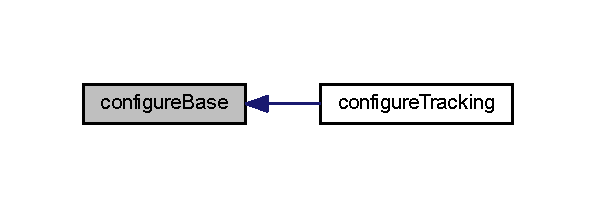
\includegraphics[width=286pt]{_pan_tilt_8h_ab7b8c8f7bf051b4f8e3b151f7b567127_icgraph}
\end{center}
\end{figure}


\hypertarget{_pan_tilt_8h_ad1d9638bad5a5021969d19769e70c775}{\index{Pan\+Tilt.\+h@{Pan\+Tilt.\+h}!get\+Dir@{get\+Dir}}
\index{get\+Dir@{get\+Dir}!Pan\+Tilt.\+h@{Pan\+Tilt.\+h}}
\subsubsection[{get\+Dir}]{\setlength{\rightskip}{0pt plus 5cm}{\bf Direction} get\+Dir (
\begin{DoxyParamCaption}
\item[{void}]{}
\end{DoxyParamCaption}
)}}\label{_pan_tilt_8h_ad1d9638bad5a5021969d19769e70c775}


 Function\+: \hyperlink{_pan_tilt_8c_ad1d9638bad5a5021969d19769e70c775}{get\+Dir(void)}

Include\+: \hyperlink{_pan_tilt_8h}{Pan\+Tilt.\+h}

Description\+: returns the current position of the pan tilt mechanism

Arguments\+: None

Returns\+: A struct containing the azimuth and inclination 

Definition at line 219 of file Pan\+Tilt.\+c.



Here is the caller graph for this function\+:\nopagebreak
\begin{figure}[H]
\begin{center}
\leavevmode
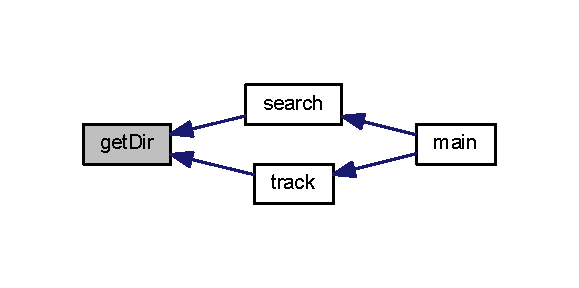
\includegraphics[width=278pt]{_pan_tilt_8h_ad1d9638bad5a5021969d19769e70c775_icgraph}
\end{center}
\end{figure}


\hypertarget{_pan_tilt_8h_ae8f9ea5919de15d1b5614be2e5e65be3}{\index{Pan\+Tilt.\+h@{Pan\+Tilt.\+h}!get\+Max\+Azimuth\+Angle@{get\+Max\+Azimuth\+Angle}}
\index{get\+Max\+Azimuth\+Angle@{get\+Max\+Azimuth\+Angle}!Pan\+Tilt.\+h@{Pan\+Tilt.\+h}}
\subsubsection[{get\+Max\+Azimuth\+Angle}]{\setlength{\rightskip}{0pt plus 5cm}char get\+Max\+Azimuth\+Angle (
\begin{DoxyParamCaption}
\item[{void}]{}
\end{DoxyParamCaption}
)}}\label{_pan_tilt_8h_ae8f9ea5919de15d1b5614be2e5e65be3}


 Function\+: \hyperlink{_pan_tilt_8c_ae8f9ea5919de15d1b5614be2e5e65be3}{get\+Max\+Azimuth\+Angle(void)}

Include\+: \hyperlink{_pan_tilt_8h}{Pan\+Tilt.\+h}

Description\+: returns the maximum angle of the azimuth servo

Arguments\+: None

Returns\+: A char with the maximum azimuth angle. 

Definition at line 235 of file Pan\+Tilt.\+c.

\hypertarget{_pan_tilt_8h_a4278dbef7fe9034a7a54d02bcbb16de9}{\index{Pan\+Tilt.\+h@{Pan\+Tilt.\+h}!get\+Max\+Elevation\+Angle@{get\+Max\+Elevation\+Angle}}
\index{get\+Max\+Elevation\+Angle@{get\+Max\+Elevation\+Angle}!Pan\+Tilt.\+h@{Pan\+Tilt.\+h}}
\subsubsection[{get\+Max\+Elevation\+Angle}]{\setlength{\rightskip}{0pt plus 5cm}char get\+Max\+Elevation\+Angle (
\begin{DoxyParamCaption}
\item[{void}]{}
\end{DoxyParamCaption}
)}}\label{_pan_tilt_8h_a4278dbef7fe9034a7a54d02bcbb16de9}


 Function\+: \hyperlink{_pan_tilt_8c_a4278dbef7fe9034a7a54d02bcbb16de9}{get\+Max\+Elevation\+Angle(void)}

Include\+: \hyperlink{_pan_tilt_8h}{Pan\+Tilt.\+h}

Description\+: returns the maximum angle of the elevation servo

Arguments\+: None

Returns\+: A char with the maximum elevation angle. 

Definition at line 267 of file Pan\+Tilt.\+c.

\hypertarget{_pan_tilt_8h_af45dd498eebe7f5ba7b228c15e7221c1}{\index{Pan\+Tilt.\+h@{Pan\+Tilt.\+h}!get\+Min\+Azimuth\+Angle@{get\+Min\+Azimuth\+Angle}}
\index{get\+Min\+Azimuth\+Angle@{get\+Min\+Azimuth\+Angle}!Pan\+Tilt.\+h@{Pan\+Tilt.\+h}}
\subsubsection[{get\+Min\+Azimuth\+Angle}]{\setlength{\rightskip}{0pt plus 5cm}char get\+Min\+Azimuth\+Angle (
\begin{DoxyParamCaption}
\item[{void}]{}
\end{DoxyParamCaption}
)}}\label{_pan_tilt_8h_af45dd498eebe7f5ba7b228c15e7221c1}


 Function\+: \hyperlink{_pan_tilt_8c_af45dd498eebe7f5ba7b228c15e7221c1}{get\+Min\+Azimuth\+Angle(void)}

Include\+: \hyperlink{_pan_tilt_8h}{Pan\+Tilt.\+h}

Description\+: returns the minimum angle of the azimuth servo

Arguments\+: None

Returns\+: A char with the minimum azimuth angle. 

Definition at line 251 of file Pan\+Tilt.\+c.

\hypertarget{_pan_tilt_8h_af7fafa63e9c645a80f28aca253bba5cc}{\index{Pan\+Tilt.\+h@{Pan\+Tilt.\+h}!get\+Min\+Elevation\+Angle@{get\+Min\+Elevation\+Angle}}
\index{get\+Min\+Elevation\+Angle@{get\+Min\+Elevation\+Angle}!Pan\+Tilt.\+h@{Pan\+Tilt.\+h}}
\subsubsection[{get\+Min\+Elevation\+Angle}]{\setlength{\rightskip}{0pt plus 5cm}char get\+Min\+Elevation\+Angle (
\begin{DoxyParamCaption}
\item[{void}]{}
\end{DoxyParamCaption}
)}}\label{_pan_tilt_8h_af7fafa63e9c645a80f28aca253bba5cc}


 Function\+: \hyperlink{_pan_tilt_8c_af7fafa63e9c645a80f28aca253bba5cc}{get\+Min\+Elevation\+Angle(void)}

Include\+: \hyperlink{_pan_tilt_8h}{Pan\+Tilt.\+h}

Description\+: returns the minimum angle of the elevation servo

Arguments\+: None

Returns\+: A char with the minimum elevation angle. 

Definition at line 283 of file Pan\+Tilt.\+c.

\hypertarget{_pan_tilt_8h_af8e57fbe1513bb48274f4f0f46717fa1}{\index{Pan\+Tilt.\+h@{Pan\+Tilt.\+h}!increment@{increment}}
\index{increment@{increment}!Pan\+Tilt.\+h@{Pan\+Tilt.\+h}}
\subsubsection[{increment}]{\setlength{\rightskip}{0pt plus 5cm}void increment (
\begin{DoxyParamCaption}
\item[{{\bf Direction}}]{difference}
\end{DoxyParamCaption}
)}}\label{_pan_tilt_8h_af8e57fbe1513bb48274f4f0f46717fa1}


 Function\+: \hyperlink{_pan_tilt_8c_af8e57fbe1513bb48274f4f0f46717fa1}{increment(\+Direction difference)}

Include\+: \hyperlink{_pan_tilt_8h}{Pan\+Tilt.\+h}

Description\+: Moves the pan tilt actuator to the specified destination

Arguments\+: destionation -\/ A struct containing the desired azimuth and inclination

Returns\+: None 

Definition at line 170 of file Pan\+Tilt.\+c.



Here is the call graph for this function\+:\nopagebreak
\begin{figure}[H]
\begin{center}
\leavevmode
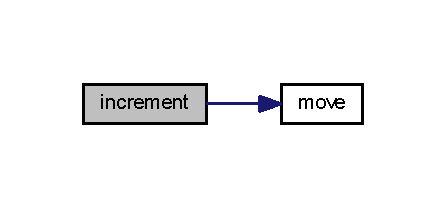
\includegraphics[width=214pt]{_pan_tilt_8h_af8e57fbe1513bb48274f4f0f46717fa1_cgraph}
\end{center}
\end{figure}




Here is the caller graph for this function\+:\nopagebreak
\begin{figure}[H]
\begin{center}
\leavevmode
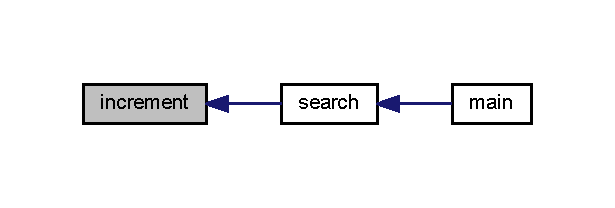
\includegraphics[width=295pt]{_pan_tilt_8h_af8e57fbe1513bb48274f4f0f46717fa1_icgraph}
\end{center}
\end{figure}


\hypertarget{_pan_tilt_8h_a5350e3f473fb25899612d382c1baa642}{\index{Pan\+Tilt.\+h@{Pan\+Tilt.\+h}!increment\+Fine@{increment\+Fine}}
\index{increment\+Fine@{increment\+Fine}!Pan\+Tilt.\+h@{Pan\+Tilt.\+h}}
\subsubsection[{increment\+Fine}]{\setlength{\rightskip}{0pt plus 5cm}void increment\+Fine (
\begin{DoxyParamCaption}
\item[{{\bf Direction}}]{difference}
\end{DoxyParamCaption}
)}}\label{_pan_tilt_8h_a5350e3f473fb25899612d382c1baa642}


 Function\+: \hyperlink{_pan_tilt_8c_a5350e3f473fb25899612d382c1baa642}{increment\+Fine(\+Direction difference)}

Include\+: \hyperlink{_pan_tilt_8h}{Pan\+Tilt.\+h}

Description\+: Moves the pan tilt actuator to the specified (Relative) destination

Arguments\+: destionation -\/ A struct containing the desired azimuth and inclination

Returns\+: None 

Definition at line 189 of file Pan\+Tilt.\+c.

\hypertarget{_pan_tilt_8h_a032fbfc434ca24d27d89b6d768455a42}{\index{Pan\+Tilt.\+h@{Pan\+Tilt.\+h}!move@{move}}
\index{move@{move}!Pan\+Tilt.\+h@{Pan\+Tilt.\+h}}
\subsubsection[{move}]{\setlength{\rightskip}{0pt plus 5cm}void move (
\begin{DoxyParamCaption}
\item[{{\bf Direction}}]{destination}
\end{DoxyParamCaption}
)}}\label{_pan_tilt_8h_a032fbfc434ca24d27d89b6d768455a42}


 Function\+: \hyperlink{_pan_tilt_8c_a032fbfc434ca24d27d89b6d768455a42}{move(\+Direction destination)}

Include\+: \hyperlink{_pan_tilt_8h}{Pan\+Tilt.\+h}

Description\+: Moves the pan tilt actuator to the specified destination

Arguments\+: destionation -\/ A struct containing the desired azimuth and inclination

Returns\+: None 

Definition at line 148 of file Pan\+Tilt.\+c.



Here is the caller graph for this function\+:\nopagebreak
\begin{figure}[H]
\begin{center}
\leavevmode
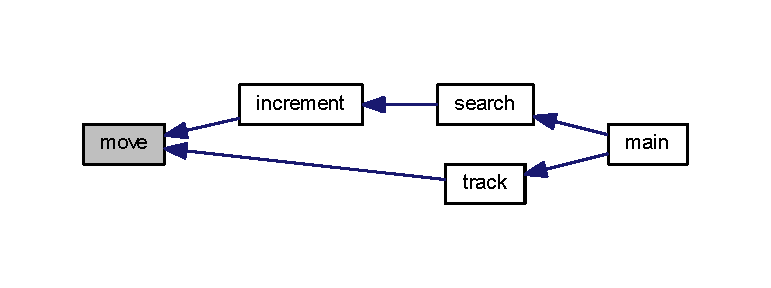
\includegraphics[width=350pt]{_pan_tilt_8h_a032fbfc434ca24d27d89b6d768455a42_icgraph}
\end{center}
\end{figure}


\hypertarget{_pan_tilt_8h_a7f353056fb02f0d95fd997198f5b186f}{\index{Pan\+Tilt.\+h@{Pan\+Tilt.\+h}!pan\+Tilt\+I\+S\+R@{pan\+Tilt\+I\+S\+R}}
\index{pan\+Tilt\+I\+S\+R@{pan\+Tilt\+I\+S\+R}!Pan\+Tilt.\+h@{Pan\+Tilt.\+h}}
\subsubsection[{pan\+Tilt\+I\+S\+R}]{\setlength{\rightskip}{0pt plus 5cm}void pan\+Tilt\+I\+S\+R (
\begin{DoxyParamCaption}
\item[{void}]{}
\end{DoxyParamCaption}
)}}\label{_pan_tilt_8h_a7f353056fb02f0d95fd997198f5b186f}


 Function\+: \hyperlink{_pan_tilt_8c_a7f353056fb02f0d95fd997198f5b186f}{pan\+Tilt\+I\+S\+R(void)}

Include\+: \hyperlink{_pan_tilt_8h}{Pan\+Tilt.\+h}

Description\+: Acts as the I\+S\+R for the Pan\+Tilt module

Arguments\+: None

Returns\+: None 

Definition at line 396 of file Pan\+Tilt.\+c.



Here is the caller graph for this function\+:\nopagebreak
\begin{figure}[H]
\begin{center}
\leavevmode
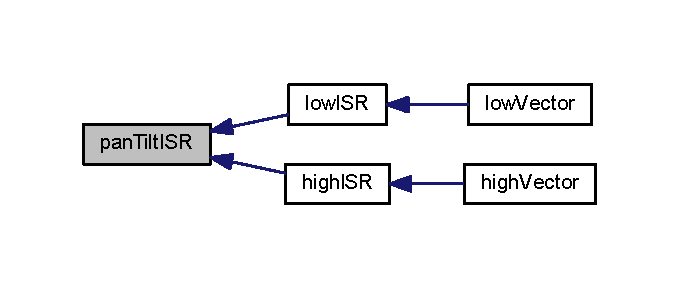
\includegraphics[width=326pt]{_pan_tilt_8h_a7f353056fb02f0d95fd997198f5b186f_icgraph}
\end{center}
\end{figure}


\hypertarget{_pan_tilt_8h_a251ee95d75c68e21c4bb933ac99e5108}{\index{Pan\+Tilt.\+h@{Pan\+Tilt.\+h}!raw\+Dir@{raw\+Dir}}
\index{raw\+Dir@{raw\+Dir}!Pan\+Tilt.\+h@{Pan\+Tilt.\+h}}
\subsubsection[{raw\+Dir}]{\setlength{\rightskip}{0pt plus 5cm}{\bf Direction} raw\+Dir (
\begin{DoxyParamCaption}
\item[{void}]{}
\end{DoxyParamCaption}
)}}\label{_pan_tilt_8h_a251ee95d75c68e21c4bb933ac99e5108}


 Function\+: \hyperlink{_pan_tilt_8c_a251ee95d75c68e21c4bb933ac99e5108}{raw\+Dir(void)}

Include\+: \hyperlink{_pan_tilt_8h}{Pan\+Tilt.\+h}

Description\+: returns the current Pan\+Tile position without calibrating

Arguments\+: None

Returns\+: The position of the pan tilt without any calibration 

Definition at line 380 of file Pan\+Tilt.\+c.

\hypertarget{_pan_tilt_8h_a1f5e600a2655aeb9dd24b8325a777931}{\index{Pan\+Tilt.\+h@{Pan\+Tilt.\+h}!set\+Max\+Azimuth\+Angle@{set\+Max\+Azimuth\+Angle}}
\index{set\+Max\+Azimuth\+Angle@{set\+Max\+Azimuth\+Angle}!Pan\+Tilt.\+h@{Pan\+Tilt.\+h}}
\subsubsection[{set\+Max\+Azimuth\+Angle}]{\setlength{\rightskip}{0pt plus 5cm}void set\+Max\+Azimuth\+Angle (
\begin{DoxyParamCaption}
\item[{char}]{p\+\_\+angle}
\end{DoxyParamCaption}
)}}\label{_pan_tilt_8h_a1f5e600a2655aeb9dd24b8325a777931}


 Function\+: set\+Max\+Azimuth\+Angle(void)

Include\+: \hyperlink{_pan_tilt_8h}{Pan\+Tilt.\+h}

Description\+: sets the maximum angle of the azimuth servo

Arguments\+: The maximum angle (as char) to set for the azimuth servo

Returns\+: None. 

Definition at line 299 of file Pan\+Tilt.\+c.

\hypertarget{_pan_tilt_8h_aa956697480994a26cb592b2cfcf3436c}{\index{Pan\+Tilt.\+h@{Pan\+Tilt.\+h}!set\+Max\+Elevation\+Angle@{set\+Max\+Elevation\+Angle}}
\index{set\+Max\+Elevation\+Angle@{set\+Max\+Elevation\+Angle}!Pan\+Tilt.\+h@{Pan\+Tilt.\+h}}
\subsubsection[{set\+Max\+Elevation\+Angle}]{\setlength{\rightskip}{0pt plus 5cm}void set\+Max\+Elevation\+Angle (
\begin{DoxyParamCaption}
\item[{char}]{p\+\_\+angle}
\end{DoxyParamCaption}
)}}\label{_pan_tilt_8h_aa956697480994a26cb592b2cfcf3436c}


 Function\+: set\+Max\+Elevation\+Angle(void)

Include\+: \hyperlink{_pan_tilt_8h}{Pan\+Tilt.\+h}

Description\+: sets the maximum angle of the elevation servo

Arguments\+: The maximum angle (as char) to set for the elevation servo

Returns\+: None. 

Definition at line 329 of file Pan\+Tilt.\+c.

\hypertarget{_pan_tilt_8h_a157ea38d68fcd31082dc2eaba2944ef3}{\index{Pan\+Tilt.\+h@{Pan\+Tilt.\+h}!set\+Min\+Azimuth\+Angle@{set\+Min\+Azimuth\+Angle}}
\index{set\+Min\+Azimuth\+Angle@{set\+Min\+Azimuth\+Angle}!Pan\+Tilt.\+h@{Pan\+Tilt.\+h}}
\subsubsection[{set\+Min\+Azimuth\+Angle}]{\setlength{\rightskip}{0pt plus 5cm}void set\+Min\+Azimuth\+Angle (
\begin{DoxyParamCaption}
\item[{char}]{p\+\_\+angle}
\end{DoxyParamCaption}
)}}\label{_pan_tilt_8h_a157ea38d68fcd31082dc2eaba2944ef3}


 Function\+: set\+Min\+Azimuth\+Angle(void)

Include\+: \hyperlink{_pan_tilt_8h}{Pan\+Tilt.\+h}

Description\+: sets the minimum angle of the azimuth servo

Arguments\+: The minimum angle (as char) to set for the azimuth servo

Returns\+: None. 

Definition at line 314 of file Pan\+Tilt.\+c.

\hypertarget{_pan_tilt_8h_a001917f3c38b200d142ab6932991e001}{\index{Pan\+Tilt.\+h@{Pan\+Tilt.\+h}!set\+Min\+Elevation\+Angle@{set\+Min\+Elevation\+Angle}}
\index{set\+Min\+Elevation\+Angle@{set\+Min\+Elevation\+Angle}!Pan\+Tilt.\+h@{Pan\+Tilt.\+h}}
\subsubsection[{set\+Min\+Elevation\+Angle}]{\setlength{\rightskip}{0pt plus 5cm}void set\+Min\+Elevation\+Angle (
\begin{DoxyParamCaption}
\item[{char}]{p\+\_\+angle}
\end{DoxyParamCaption}
)}}\label{_pan_tilt_8h_a001917f3c38b200d142ab6932991e001}


 Function\+: set\+Min\+Elevation\+Angle(void)

Include\+: \hyperlink{_pan_tilt_8h}{Pan\+Tilt.\+h}

Description\+: sets the minimum angle of the elevation servo

Arguments\+: The minimum angle (as char) to set for the elevation servo

Returns\+: None. 

Definition at line 345 of file Pan\+Tilt.\+c.

\hypertarget{_pan_tilt_8h_a3362a0aacdd7037d0329989d353c60b7}{\index{Pan\+Tilt.\+h@{Pan\+Tilt.\+h}!updated@{updated}}
\index{updated@{updated}!Pan\+Tilt.\+h@{Pan\+Tilt.\+h}}
\subsubsection[{updated}]{\setlength{\rightskip}{0pt plus 5cm}char updated (
\begin{DoxyParamCaption}
\item[{void}]{}
\end{DoxyParamCaption}
)}}\label{_pan_tilt_8h_a3362a0aacdd7037d0329989d353c60b7}


 Function\+: \hyperlink{_pan_tilt_8c_a3362a0aacdd7037d0329989d353c60b7}{updated(void)}

Include\+: \hyperlink{_pan_tilt_8h}{Pan\+Tilt.\+h}

Description\+: returns true if the last move or increment or increment\+Fine function has taken effect. The new direction is only loaded in at the end of the P\+D\+M, so it could take up to 0.\+02 seconds for the change to take effect.

Arguments\+: delay -\/ a pointer to the delay variable

Returns\+: None 

Definition at line 532 of file Pan\+Tilt.\+c.


\hypertarget{_range_8c}{\section{Range.\+c File Reference}
\label{_range_8c}\index{Range.\+c@{Range.\+c}}
}
{\ttfamily \#include \char`\"{}Common.\+h\char`\"{}}\\*
{\ttfamily \#include \char`\"{}Temp.\+h\char`\"{}}\\*
Include dependency graph for Range.\+c\+:\nopagebreak
\begin{figure}[H]
\begin{center}
\leavevmode
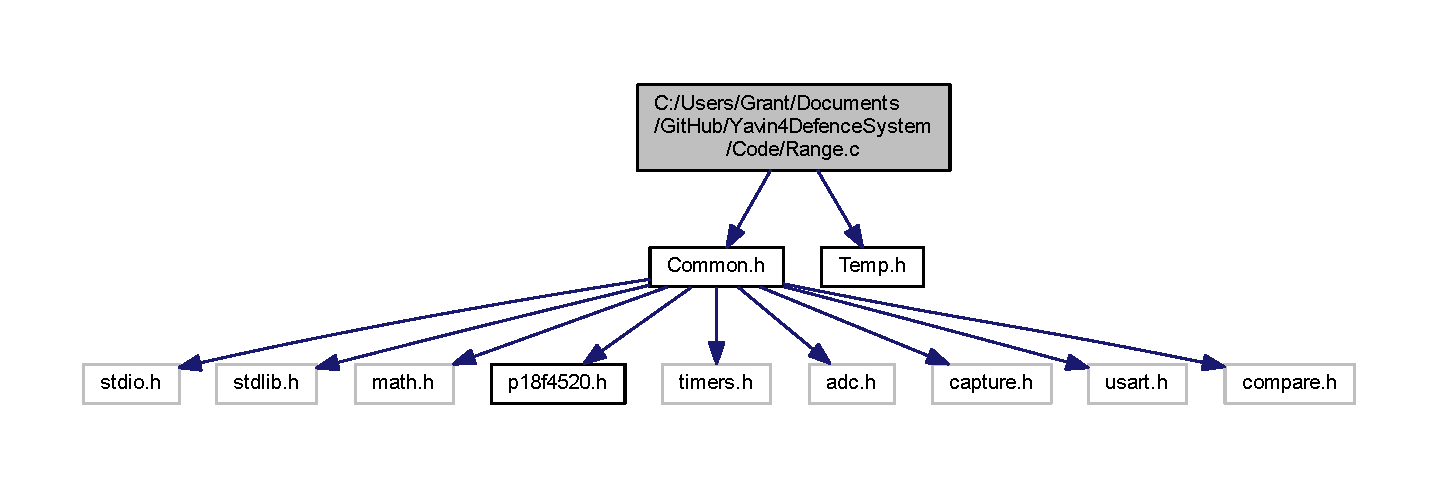
\includegraphics[width=350pt]{_range_8c__incl}
\end{center}
\end{figure}
\subsection*{Macros}
\begin{DoxyCompactItemize}
\item 
\#define \hyperlink{_range_8c_a8dce7331368588b9016a33f044b71d91}{S\+P\+D\+\_\+\+S\+N\+D}(T)~(\hyperlink{_common_8h_a740656a5f724d0a99e528def8ce50125}{D\+I\+V\+\_\+1024}(T $\ast$ (unsigned int)614) + 331)
\item 
\#define \hyperlink{_range_8c_a13235bb583d24031d4129a10c126ef8e}{I\+R\+\_\+\+C\+O\+N\+V}(ad)~((unsigned long)135174 / (ad) -\/ 28)
\item 
\#define \hyperlink{_range_8c_a354db24d9e733cf8b3e15f727ab46624}{U\+L\+T\+R\+A\+\_\+\+C\+O\+N\+V}(tme, T)~\hyperlink{_common_8h_a9469c415aff989522dac534ab8adb35e}{D\+I\+V\+\_\+65536}(tme $\ast$ (unsigned long)(\hyperlink{_common_8h_a9469c415aff989522dac534ab8adb35e}{D\+I\+V\+\_\+65536}((unsigned long)519078 $\ast$ T) + (unsigned long)4362)) -\/ 18
\item 
\#define \hyperlink{_range_8c_acf4b9381566c4a7de8b59886038b9132}{N\+U\+M\+\_\+\+I\+R\+\_\+\+R\+E\+A\+D\+S}~10
\item 
\#define \hyperlink{_range_8c_a885e4c51dcc91fcae14dadc2d564f270}{I\+N\+I\+T\+\_\+\+P\+I\+N}~\hyperlink{p18f4520_8h_ae6cab3544e1e4b7eaec41046bf007800}{P\+O\+R\+T\+Cbits.\+R\+C3}
\item 
\#define \hyperlink{_range_8c_a6e6430371976f713ccccb6372b19b810}{I\+N\+I\+T\+\_\+\+T\+R\+I\+S}~\hyperlink{p18f4520_8h_ae6cab3544e1e4b7eaec41046bf007800}{T\+R\+I\+S\+Cbits.\+R\+C3}
\item 
\#define \hyperlink{_range_8c_aa42da5a67cdb563f37b56c1674dd67bb}{C\+C\+P1\+\_\+\+I\+N\+P\+T}~\hyperlink{p18f4520_8h_a2155381890524f46a1a03878e5f52682}{T\+R\+I\+S\+Cbits.\+R\+C2}
\end{DoxyCompactItemize}
\subsection*{Functions}
\begin{DoxyCompactItemize}
\item 
unsigned int \hyperlink{_range_8c_a91b55894b9e6d74e4495ea610246c856}{range\+I\+R} (void)
\item 
void \hyperlink{_range_8c_a07a4c592815b5e6ae178f93a7764ceb2}{configure\+Range} (void)
\item 
void \hyperlink{_range_8c_ac7337ef2da4c9ab03257562ec33bbb8a}{configure\+A\+D} (void)
\item 
void \hyperlink{_range_8c_a64e9d21d140ac54a306dab455b49adcf}{range\+I\+S\+R} (void)
\item 
void \hyperlink{_range_8c_a8606bd1052dde0e7c32eddad8699f4f4}{calibrate\+Range} (unsigned int reference)
\item 
unsigned int \hyperlink{_range_8c_a90ce8835c75e17b8e2d15eca3e6ae82f}{raw\+Range} (void)
\item 
unsigned int \hyperlink{_range_8c_aff3698f3a7b3b5963d8e6b305a165d71}{range} (void)
\item 
unsigned int \hyperlink{_range_8c_a5b063989d39d2958d2ecebc0106cb1da}{range\+Ultrasonic} (void)
\item 
\hyperlink{_common_8h_a2db986326a654991cce9b1c2b1670677}{Target\+State} \hyperlink{_range_8c_a3e5554f5a076ded63b937d50b7e5c9db}{get\+Target\+State} (void)
\item 
\hyperlink{_common_8h_a2db986326a654991cce9b1c2b1670677}{Target\+State} \hyperlink{_range_8c_a87c8e64ddc596f3e6b72ee861f671168}{read\+Target\+State} (void)
\end{DoxyCompactItemize}


\subsection{Macro Definition Documentation}
\hypertarget{_range_8c_aa42da5a67cdb563f37b56c1674dd67bb}{\index{Range.\+c@{Range.\+c}!C\+C\+P1\+\_\+\+I\+N\+P\+T@{C\+C\+P1\+\_\+\+I\+N\+P\+T}}
\index{C\+C\+P1\+\_\+\+I\+N\+P\+T@{C\+C\+P1\+\_\+\+I\+N\+P\+T}!Range.\+c@{Range.\+c}}
\subsubsection[{C\+C\+P1\+\_\+\+I\+N\+P\+T}]{\setlength{\rightskip}{0pt plus 5cm}\#define C\+C\+P1\+\_\+\+I\+N\+P\+T~{\bf T\+R\+I\+S\+Cbits.\+R\+C2}}}\label{_range_8c_aa42da5a67cdb563f37b56c1674dd67bb}


Definition at line 40 of file Range.\+c.

\hypertarget{_range_8c_a885e4c51dcc91fcae14dadc2d564f270}{\index{Range.\+c@{Range.\+c}!I\+N\+I\+T\+\_\+\+P\+I\+N@{I\+N\+I\+T\+\_\+\+P\+I\+N}}
\index{I\+N\+I\+T\+\_\+\+P\+I\+N@{I\+N\+I\+T\+\_\+\+P\+I\+N}!Range.\+c@{Range.\+c}}
\subsubsection[{I\+N\+I\+T\+\_\+\+P\+I\+N}]{\setlength{\rightskip}{0pt plus 5cm}\#define I\+N\+I\+T\+\_\+\+P\+I\+N~{\bf P\+O\+R\+T\+Cbits.\+R\+C3}}}\label{_range_8c_a885e4c51dcc91fcae14dadc2d564f270}


Definition at line 38 of file Range.\+c.

\hypertarget{_range_8c_a6e6430371976f713ccccb6372b19b810}{\index{Range.\+c@{Range.\+c}!I\+N\+I\+T\+\_\+\+T\+R\+I\+S@{I\+N\+I\+T\+\_\+\+T\+R\+I\+S}}
\index{I\+N\+I\+T\+\_\+\+T\+R\+I\+S@{I\+N\+I\+T\+\_\+\+T\+R\+I\+S}!Range.\+c@{Range.\+c}}
\subsubsection[{I\+N\+I\+T\+\_\+\+T\+R\+I\+S}]{\setlength{\rightskip}{0pt plus 5cm}\#define I\+N\+I\+T\+\_\+\+T\+R\+I\+S~{\bf T\+R\+I\+S\+Cbits.\+R\+C3}}}\label{_range_8c_a6e6430371976f713ccccb6372b19b810}


Definition at line 39 of file Range.\+c.

\hypertarget{_range_8c_a13235bb583d24031d4129a10c126ef8e}{\index{Range.\+c@{Range.\+c}!I\+R\+\_\+\+C\+O\+N\+V@{I\+R\+\_\+\+C\+O\+N\+V}}
\index{I\+R\+\_\+\+C\+O\+N\+V@{I\+R\+\_\+\+C\+O\+N\+V}!Range.\+c@{Range.\+c}}
\subsubsection[{I\+R\+\_\+\+C\+O\+N\+V}]{\setlength{\rightskip}{0pt plus 5cm}\#define I\+R\+\_\+\+C\+O\+N\+V(
\begin{DoxyParamCaption}
\item[{}]{ad}
\end{DoxyParamCaption}
)~((unsigned long)135174 / (ad) -\/ 28)}}\label{_range_8c_a13235bb583d24031d4129a10c126ef8e}


Definition at line 27 of file Range.\+c.

\hypertarget{_range_8c_acf4b9381566c4a7de8b59886038b9132}{\index{Range.\+c@{Range.\+c}!N\+U\+M\+\_\+\+I\+R\+\_\+\+R\+E\+A\+D\+S@{N\+U\+M\+\_\+\+I\+R\+\_\+\+R\+E\+A\+D\+S}}
\index{N\+U\+M\+\_\+\+I\+R\+\_\+\+R\+E\+A\+D\+S@{N\+U\+M\+\_\+\+I\+R\+\_\+\+R\+E\+A\+D\+S}!Range.\+c@{Range.\+c}}
\subsubsection[{N\+U\+M\+\_\+\+I\+R\+\_\+\+R\+E\+A\+D\+S}]{\setlength{\rightskip}{0pt plus 5cm}\#define N\+U\+M\+\_\+\+I\+R\+\_\+\+R\+E\+A\+D\+S~10}}\label{_range_8c_acf4b9381566c4a7de8b59886038b9132}


Definition at line 35 of file Range.\+c.

\hypertarget{_range_8c_a8dce7331368588b9016a33f044b71d91}{\index{Range.\+c@{Range.\+c}!S\+P\+D\+\_\+\+S\+N\+D@{S\+P\+D\+\_\+\+S\+N\+D}}
\index{S\+P\+D\+\_\+\+S\+N\+D@{S\+P\+D\+\_\+\+S\+N\+D}!Range.\+c@{Range.\+c}}
\subsubsection[{S\+P\+D\+\_\+\+S\+N\+D}]{\setlength{\rightskip}{0pt plus 5cm}\#define S\+P\+D\+\_\+\+S\+N\+D(
\begin{DoxyParamCaption}
\item[{}]{T}
\end{DoxyParamCaption}
)~({\bf D\+I\+V\+\_\+1024}(T $\ast$ (unsigned int)614) + 331)}}\label{_range_8c_a8dce7331368588b9016a33f044b71d91}


 File\+: \hyperlink{_range_8c}{Range.\+c} Author\+: Grant

Description\+: Contains all the functionality for the range module. All variables and settings concerning the range module including the the max distance, timeouts etc are private to this module. The interface functions allow all valid access to the module.

Duties\+: -\/\+Interface to the I\+R and Ultrasonic sensors -\/\+Read the range from the I\+R and ultrasonic sensors -\/\+Fuse distances from the I\+R and ultrasonic sensors -\/\+Calibrate the I\+R and ultrasonic sensors

Functions\+:

Created on 15 September 2014, 11\+:27 A\+M 

Definition at line 26 of file Range.\+c.

\hypertarget{_range_8c_a354db24d9e733cf8b3e15f727ab46624}{\index{Range.\+c@{Range.\+c}!U\+L\+T\+R\+A\+\_\+\+C\+O\+N\+V@{U\+L\+T\+R\+A\+\_\+\+C\+O\+N\+V}}
\index{U\+L\+T\+R\+A\+\_\+\+C\+O\+N\+V@{U\+L\+T\+R\+A\+\_\+\+C\+O\+N\+V}!Range.\+c@{Range.\+c}}
\subsubsection[{U\+L\+T\+R\+A\+\_\+\+C\+O\+N\+V}]{\setlength{\rightskip}{0pt plus 5cm}\#define U\+L\+T\+R\+A\+\_\+\+C\+O\+N\+V(
\begin{DoxyParamCaption}
\item[{}]{tme, }
\item[{}]{T}
\end{DoxyParamCaption}
)~{\bf D\+I\+V\+\_\+65536}(tme $\ast$ (unsigned long)({\bf D\+I\+V\+\_\+65536}((unsigned long)519078 $\ast$ T) + (unsigned long)4362)) -\/ 18}}\label{_range_8c_a354db24d9e733cf8b3e15f727ab46624}


Definition at line 30 of file Range.\+c.



\subsection{Function Documentation}
\hypertarget{_range_8c_a8606bd1052dde0e7c32eddad8699f4f4}{\index{Range.\+c@{Range.\+c}!calibrate\+Range@{calibrate\+Range}}
\index{calibrate\+Range@{calibrate\+Range}!Range.\+c@{Range.\+c}}
\subsubsection[{calibrate\+Range}]{\setlength{\rightskip}{0pt plus 5cm}void calibrate\+Range (
\begin{DoxyParamCaption}
\item[{unsigned int}]{reference}
\end{DoxyParamCaption}
)}}\label{_range_8c_a8606bd1052dde0e7c32eddad8699f4f4}


 Function\+: \hyperlink{_range_8c_a8606bd1052dde0e7c32eddad8699f4f4}{calibrate\+Range(unsigned int reference)}

Include\+:

Description\+: Calibrates the range of both the I\+R and ultrasonic sensors based on a given range.

Arguments\+: reference -\/ The distance in mm to calibrate the current measurements from

Returns\+: None 

Definition at line 251 of file Range.\+c.



Here is the call graph for this function\+:\nopagebreak
\begin{figure}[H]
\begin{center}
\leavevmode
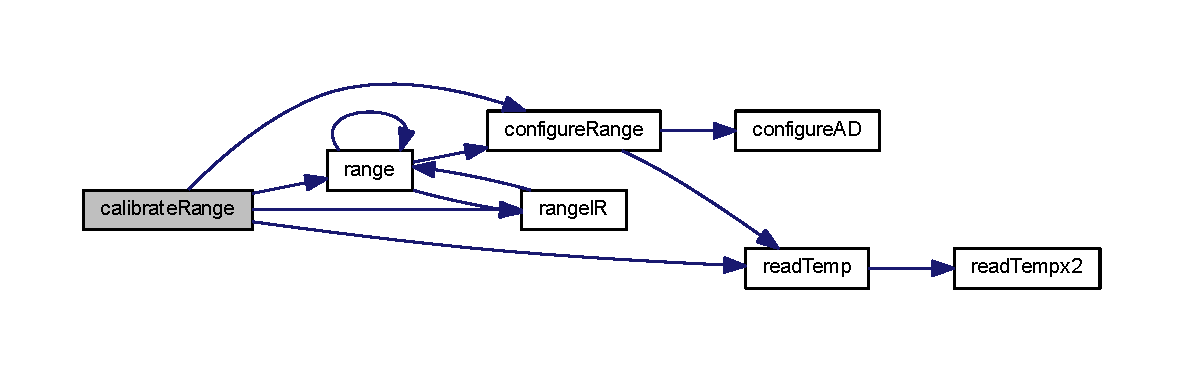
\includegraphics[width=350pt]{_range_8c_a8606bd1052dde0e7c32eddad8699f4f4_cgraph}
\end{center}
\end{figure}


\hypertarget{_range_8c_ac7337ef2da4c9ab03257562ec33bbb8a}{\index{Range.\+c@{Range.\+c}!configure\+A\+D@{configure\+A\+D}}
\index{configure\+A\+D@{configure\+A\+D}!Range.\+c@{Range.\+c}}
\subsubsection[{configure\+A\+D}]{\setlength{\rightskip}{0pt plus 5cm}void configure\+A\+D (
\begin{DoxyParamCaption}
\item[{void}]{}
\end{DoxyParamCaption}
)}}\label{_range_8c_ac7337ef2da4c9ab03257562ec33bbb8a}


 Function\+: \hyperlink{_range_8c_ac7337ef2da4c9ab03257562ec33bbb8a}{configure\+A\+D(void)}

Include\+: \hyperlink{_range_8h}{Range.\+h}

Description\+: Configures the A\+D\+C, In A\+D\+C\+O\+N1, we set right-\/justified mode, and select A\+N0 as the input channel. In A\+D\+C\+O\+N0, we set a sample rate of Fosc/8, select A\+N0, and enable the A\+D\+C. Arguments\+: None

Returns\+: None 

Definition at line 78 of file Range.\+c.



Here is the caller graph for this function\+:\nopagebreak
\begin{figure}[H]
\begin{center}
\leavevmode
\includegraphics[width=350pt]{_range_8c_ac7337ef2da4c9ab03257562ec33bbb8a_icgraph}
\end{center}
\end{figure}


\hypertarget{_range_8c_a07a4c592815b5e6ae178f93a7764ceb2}{\index{Range.\+c@{Range.\+c}!configure\+Range@{configure\+Range}}
\index{configure\+Range@{configure\+Range}!Range.\+c@{Range.\+c}}
\subsubsection[{configure\+Range}]{\setlength{\rightskip}{0pt plus 5cm}void configure\+Range (
\begin{DoxyParamCaption}
\item[{void}]{}
\end{DoxyParamCaption}
)}}\label{_range_8c_a07a4c592815b5e6ae178f93a7764ceb2}


 Function\+: \hyperlink{_range_8c_a07a4c592815b5e6ae178f93a7764ceb2}{configure\+Range(void)}

Include\+: \hyperlink{_range_8h}{Range.\+h}

Description\+: Configures the Range module

Arguments\+: None

Returns\+: None 

Definition at line 102 of file Range.\+c.



Here is the call graph for this function\+:\nopagebreak
\begin{figure}[H]
\begin{center}
\leavevmode
\includegraphics[width=350pt]{_range_8c_a07a4c592815b5e6ae178f93a7764ceb2_cgraph}
\end{center}
\end{figure}




Here is the caller graph for this function\+:\nopagebreak
\begin{figure}[H]
\begin{center}
\leavevmode
\includegraphics[width=350pt]{_range_8c_a07a4c592815b5e6ae178f93a7764ceb2_icgraph}
\end{center}
\end{figure}


\hypertarget{_range_8c_a3e5554f5a076ded63b937d50b7e5c9db}{\index{Range.\+c@{Range.\+c}!get\+Target\+State@{get\+Target\+State}}
\index{get\+Target\+State@{get\+Target\+State}!Range.\+c@{Range.\+c}}
\subsubsection[{get\+Target\+State}]{\setlength{\rightskip}{0pt plus 5cm}{\bf Target\+State} get\+Target\+State (
\begin{DoxyParamCaption}
\item[{void}]{}
\end{DoxyParamCaption}
)}}\label{_range_8c_a3e5554f5a076ded63b937d50b7e5c9db}


 Function\+: \hyperlink{_range_8c_a3e5554f5a076ded63b937d50b7e5c9db}{get\+Target\+State(void)}

Include\+: \hyperlink{_range_8h}{Range.\+h}

Description\+: Returns the target state from the last range reading. E.\+g. Good track, or direction not quite correct as U\+S returned, but I\+R didn't and was within I\+R range etc.

Arguments\+: None

Returns\+: the target state 

Definition at line 499 of file Range.\+c.



Here is the caller graph for this function\+:\nopagebreak
\begin{figure}[H]
\begin{center}
\leavevmode
\includegraphics[width=350pt]{_range_8c_a3e5554f5a076ded63b937d50b7e5c9db_icgraph}
\end{center}
\end{figure}


\hypertarget{_range_8c_aff3698f3a7b3b5963d8e6b305a165d71}{\index{Range.\+c@{Range.\+c}!range@{range}}
\index{range@{range}!Range.\+c@{Range.\+c}}
\subsubsection[{range}]{\setlength{\rightskip}{0pt plus 5cm}unsigned int range (
\begin{DoxyParamCaption}
\item[{void}]{}
\end{DoxyParamCaption}
)}}\label{_range_8c_aff3698f3a7b3b5963d8e6b305a165d71}


 Function\+: \hyperlink{_range_8c_aff3698f3a7b3b5963d8e6b305a165d71}{range()}

Include\+:

Description\+: Uses the I\+R and Ultrasonic sensors to find the range

Arguments\+: None

Returns\+: None 

Definition at line 307 of file Range.\+c.



Here is the call graph for this function\+:\nopagebreak
\begin{figure}[H]
\begin{center}
\leavevmode
\includegraphics[width=350pt]{_range_8c_aff3698f3a7b3b5963d8e6b305a165d71_cgraph}
\end{center}
\end{figure}




Here is the caller graph for this function\+:\nopagebreak
\begin{figure}[H]
\begin{center}
\leavevmode
\includegraphics[width=350pt]{_range_8c_aff3698f3a7b3b5963d8e6b305a165d71_icgraph}
\end{center}
\end{figure}


\hypertarget{_range_8c_a91b55894b9e6d74e4495ea610246c856}{\index{Range.\+c@{Range.\+c}!range\+I\+R@{range\+I\+R}}
\index{range\+I\+R@{range\+I\+R}!Range.\+c@{Range.\+c}}
\subsubsection[{range\+I\+R}]{\setlength{\rightskip}{0pt plus 5cm}unsigned int range\+I\+R (
\begin{DoxyParamCaption}
\item[{void}]{}
\end{DoxyParamCaption}
)}}\label{_range_8c_a91b55894b9e6d74e4495ea610246c856}


 Function\+: \hyperlink{_range_8c_a91b55894b9e6d74e4495ea610246c856}{range\+I\+R(void)}

Include\+:

Description\+: Reads the range from the I\+R Sensor

Arguments\+: None

Returns\+: Range (in mm) as an unsigned int.

Remark\+: Returns 0 if there is no target found 

Definition at line 406 of file Range.\+c.



Here is the call graph for this function\+:\nopagebreak
\begin{figure}[H]
\begin{center}
\leavevmode
\includegraphics[width=350pt]{_range_8c_a91b55894b9e6d74e4495ea610246c856_cgraph}
\end{center}
\end{figure}




Here is the caller graph for this function\+:\nopagebreak
\begin{figure}[H]
\begin{center}
\leavevmode
\includegraphics[width=350pt]{_range_8c_a91b55894b9e6d74e4495ea610246c856_icgraph}
\end{center}
\end{figure}


\hypertarget{_range_8c_a64e9d21d140ac54a306dab455b49adcf}{\index{Range.\+c@{Range.\+c}!range\+I\+S\+R@{range\+I\+S\+R}}
\index{range\+I\+S\+R@{range\+I\+S\+R}!Range.\+c@{Range.\+c}}
\subsubsection[{range\+I\+S\+R}]{\setlength{\rightskip}{0pt plus 5cm}void range\+I\+S\+R (
\begin{DoxyParamCaption}
\item[{void}]{}
\end{DoxyParamCaption}
)}}\label{_range_8c_a64e9d21d140ac54a306dab455b49adcf}


 Function\+: \hyperlink{_range_8c_a64e9d21d140ac54a306dab455b49adcf}{range\+I\+S\+R(void)}

Include\+: ultrasonic.\+h

Description\+: Called when an range related interrupt is fired, acts as the service routine for the rangefinding module.

Arguments\+: None

Returns\+: None 

Definition at line 219 of file Range.\+c.



Here is the caller graph for this function\+:\nopagebreak
\begin{figure}[H]
\begin{center}
\leavevmode
\includegraphics[width=321pt]{_range_8c_a64e9d21d140ac54a306dab455b49adcf_icgraph}
\end{center}
\end{figure}


\hypertarget{_range_8c_a5b063989d39d2958d2ecebc0106cb1da}{\index{Range.\+c@{Range.\+c}!range\+Ultrasonic@{range\+Ultrasonic}}
\index{range\+Ultrasonic@{range\+Ultrasonic}!Range.\+c@{Range.\+c}}
\subsubsection[{range\+Ultrasonic}]{\setlength{\rightskip}{0pt plus 5cm}unsigned int range\+Ultrasonic (
\begin{DoxyParamCaption}
\item[{void}]{}
\end{DoxyParamCaption}
)}}\label{_range_8c_a5b063989d39d2958d2ecebc0106cb1da}


 Function\+: range\+U\+S(void)

Include\+:

Description\+: performs an ultrasonic range reading. Pins\+:

Arguments\+: None

Returns\+: the average of the samples 

Definition at line 434 of file Range.\+c.



Here is the call graph for this function\+:\nopagebreak
\begin{figure}[H]
\begin{center}
\leavevmode
\includegraphics[width=350pt]{_range_8c_a5b063989d39d2958d2ecebc0106cb1da_cgraph}
\end{center}
\end{figure}


\hypertarget{_range_8c_a90ce8835c75e17b8e2d15eca3e6ae82f}{\index{Range.\+c@{Range.\+c}!raw\+Range@{raw\+Range}}
\index{raw\+Range@{raw\+Range}!Range.\+c@{Range.\+c}}
\subsubsection[{raw\+Range}]{\setlength{\rightskip}{0pt plus 5cm}unsigned int raw\+Range (
\begin{DoxyParamCaption}
\item[{void}]{}
\end{DoxyParamCaption}
)}}\label{_range_8c_a90ce8835c75e17b8e2d15eca3e6ae82f}


 Function\+: speed\+\_\+sound(unsigned char tempx2)

Include\+:

Description\+: Returns the calibration offset to calculate the raw data

Arguments\+: None

Returns\+: None 

Definition at line 291 of file Range.\+c.

\hypertarget{_range_8c_a87c8e64ddc596f3e6b72ee861f671168}{\index{Range.\+c@{Range.\+c}!read\+Target\+State@{read\+Target\+State}}
\index{read\+Target\+State@{read\+Target\+State}!Range.\+c@{Range.\+c}}
\subsubsection[{read\+Target\+State}]{\setlength{\rightskip}{0pt plus 5cm}{\bf Target\+State} read\+Target\+State (
\begin{DoxyParamCaption}
\item[{void}]{}
\end{DoxyParamCaption}
)}}\label{_range_8c_a87c8e64ddc596f3e6b72ee861f671168}


 Function\+: \hyperlink{_range_8c_a87c8e64ddc596f3e6b72ee861f671168}{read\+Target\+State(void)}

Include\+: \hyperlink{_range_8h}{Range.\+h}

Description\+: Does the same thing as get\+Target\+State, but actually performs a \hyperlink{_range_8c_aff3698f3a7b3b5963d8e6b305a165d71}{range()} read

Arguments\+: None

Returns\+: the target state 

Definition at line 516 of file Range.\+c.



Here is the call graph for this function\+:\nopagebreak
\begin{figure}[H]
\begin{center}
\leavevmode
\includegraphics[width=350pt]{_range_8c_a87c8e64ddc596f3e6b72ee861f671168_cgraph}
\end{center}
\end{figure}




Here is the caller graph for this function\+:\nopagebreak
\begin{figure}[H]
\begin{center}
\leavevmode
\includegraphics[width=322pt]{_range_8c_a87c8e64ddc596f3e6b72ee861f671168_icgraph}
\end{center}
\end{figure}



\hypertarget{_range_8h}{\section{Range.\+h File Reference}
\label{_range_8h}\index{Range.\+h@{Range.\+h}}
}
This graph shows which files directly or indirectly include this file\+:
\nopagebreak
\begin{figure}[H]
\begin{center}
\leavevmode
\includegraphics[width=307pt]{_range_8h__dep__incl}
\end{center}
\end{figure}
\subsection*{Macros}
\begin{DoxyCompactItemize}
\item 
\#define \hyperlink{_range_8h_acbdd28592e68851fc99aa81a3b917fc9}{R\+A\+N\+G\+E\+\_\+\+I\+N\+T}~\hyperlink{_common_8h_a1673a1a80febeafd51f3f02508a0ea71}{C\+C\+P1\+\_\+\+I\+N\+T} $\vert$ \hyperlink{_common_8h_af1b5f2499fdbb5b83800325b12a062cf}{T\+M\+R1\+\_\+\+I\+N\+T}
\end{DoxyCompactItemize}
\subsection*{Functions}
\begin{DoxyCompactItemize}
\item 
void \hyperlink{_range_8h_a07a4c592815b5e6ae178f93a7764ceb2}{configure\+Range} (void)
\item 
void \hyperlink{_range_8h_ac7337ef2da4c9ab03257562ec33bbb8a}{configure\+A\+D} (void)
\item 
unsigned int \hyperlink{_range_8h_aff3698f3a7b3b5963d8e6b305a165d71}{range} (void)
\item 
void \hyperlink{_range_8h_a64e9d21d140ac54a306dab455b49adcf}{range\+I\+S\+R} (void)
\item 
void \hyperlink{_range_8h_ae2fb7c6f16c048f7f3247b7b5a3d403a}{calibrate\+Range} (signed int distance)
\item 
signed int \hyperlink{_range_8h_a2c0a42fe463e1d8bd954fe3679aef5c2}{raw\+Range} (void)
\item 
\hyperlink{_common_8h_a2db986326a654991cce9b1c2b1670677}{Target\+State} \hyperlink{_range_8h_a3e5554f5a076ded63b937d50b7e5c9db}{get\+Target\+State} (void)
\item 
\hyperlink{_common_8h_a2db986326a654991cce9b1c2b1670677}{Target\+State} \hyperlink{_range_8h_a87c8e64ddc596f3e6b72ee861f671168}{read\+Target\+State} (void)
\item 
unsigned int \hyperlink{_range_8h_a91b55894b9e6d74e4495ea610246c856}{range\+I\+R} (void)
\item 
unsigned int \hyperlink{_range_8h_a5b063989d39d2958d2ecebc0106cb1da}{range\+Ultrasonic} (void)
\end{DoxyCompactItemize}


\subsection{Macro Definition Documentation}
\hypertarget{_range_8h_acbdd28592e68851fc99aa81a3b917fc9}{\index{Range.\+h@{Range.\+h}!R\+A\+N\+G\+E\+\_\+\+I\+N\+T@{R\+A\+N\+G\+E\+\_\+\+I\+N\+T}}
\index{R\+A\+N\+G\+E\+\_\+\+I\+N\+T@{R\+A\+N\+G\+E\+\_\+\+I\+N\+T}!Range.\+h@{Range.\+h}}
\subsubsection[{R\+A\+N\+G\+E\+\_\+\+I\+N\+T}]{\setlength{\rightskip}{0pt plus 5cm}\#define R\+A\+N\+G\+E\+\_\+\+I\+N\+T~{\bf C\+C\+P1\+\_\+\+I\+N\+T} $\vert$ {\bf T\+M\+R1\+\_\+\+I\+N\+T}}}\label{_range_8h_acbdd28592e68851fc99aa81a3b917fc9}


Definition at line 12 of file Range.\+h.



\subsection{Function Documentation}
\hypertarget{_range_8h_ae2fb7c6f16c048f7f3247b7b5a3d403a}{\index{Range.\+h@{Range.\+h}!calibrate\+Range@{calibrate\+Range}}
\index{calibrate\+Range@{calibrate\+Range}!Range.\+h@{Range.\+h}}
\subsubsection[{calibrate\+Range}]{\setlength{\rightskip}{0pt plus 5cm}void calibrate\+Range (
\begin{DoxyParamCaption}
\item[{signed int}]{distance}
\end{DoxyParamCaption}
)}}\label{_range_8h_ae2fb7c6f16c048f7f3247b7b5a3d403a}
\hypertarget{_range_8h_ac7337ef2da4c9ab03257562ec33bbb8a}{\index{Range.\+h@{Range.\+h}!configure\+A\+D@{configure\+A\+D}}
\index{configure\+A\+D@{configure\+A\+D}!Range.\+h@{Range.\+h}}
\subsubsection[{configure\+A\+D}]{\setlength{\rightskip}{0pt plus 5cm}void configure\+A\+D (
\begin{DoxyParamCaption}
\item[{void}]{}
\end{DoxyParamCaption}
)}}\label{_range_8h_ac7337ef2da4c9ab03257562ec33bbb8a}


 Function\+: \hyperlink{_range_8c_ac7337ef2da4c9ab03257562ec33bbb8a}{configure\+A\+D(void)}

Include\+: \hyperlink{_range_8h}{Range.\+h}

Description\+: Configures the A\+D\+C, In A\+D\+C\+O\+N1, we set right-\/justified mode, and select A\+N0 as the input channel. In A\+D\+C\+O\+N0, we set a sample rate of Fosc/8, select A\+N0, and enable the A\+D\+C. Arguments\+: None

Returns\+: None 

Definition at line 69 of file Range.\+c.



Here is the caller graph for this function\+:
\nopagebreak
\begin{figure}[H]
\begin{center}
\leavevmode
\includegraphics[width=350pt]{_range_8h_ac7337ef2da4c9ab03257562ec33bbb8a_icgraph}
\end{center}
\end{figure}


\hypertarget{_range_8h_a07a4c592815b5e6ae178f93a7764ceb2}{\index{Range.\+h@{Range.\+h}!configure\+Range@{configure\+Range}}
\index{configure\+Range@{configure\+Range}!Range.\+h@{Range.\+h}}
\subsubsection[{configure\+Range}]{\setlength{\rightskip}{0pt plus 5cm}void configure\+Range (
\begin{DoxyParamCaption}
\item[{void}]{}
\end{DoxyParamCaption}
)}}\label{_range_8h_a07a4c592815b5e6ae178f93a7764ceb2}


 Function\+: \hyperlink{_range_8c_a07a4c592815b5e6ae178f93a7764ceb2}{configure\+Range(void)}

Include\+: \hyperlink{_range_8h}{Range.\+h}

Description\+: Configures the Range module

Arguments\+: None

Returns\+: None 

Definition at line 93 of file Range.\+c.



Here is the call graph for this function\+:
\nopagebreak
\begin{figure}[H]
\begin{center}
\leavevmode
\includegraphics[width=350pt]{_range_8h_a07a4c592815b5e6ae178f93a7764ceb2_cgraph}
\end{center}
\end{figure}




Here is the caller graph for this function\+:
\nopagebreak
\begin{figure}[H]
\begin{center}
\leavevmode
\includegraphics[width=350pt]{_range_8h_a07a4c592815b5e6ae178f93a7764ceb2_icgraph}
\end{center}
\end{figure}


\hypertarget{_range_8h_a3e5554f5a076ded63b937d50b7e5c9db}{\index{Range.\+h@{Range.\+h}!get\+Target\+State@{get\+Target\+State}}
\index{get\+Target\+State@{get\+Target\+State}!Range.\+h@{Range.\+h}}
\subsubsection[{get\+Target\+State}]{\setlength{\rightskip}{0pt plus 5cm}{\bf Target\+State} get\+Target\+State (
\begin{DoxyParamCaption}
\item[{void}]{}
\end{DoxyParamCaption}
)}}\label{_range_8h_a3e5554f5a076ded63b937d50b7e5c9db}


 Function\+: \hyperlink{_range_8c_a3e5554f5a076ded63b937d50b7e5c9db}{get\+Target\+State(void)}

Include\+: \hyperlink{_range_8h}{Range.\+h}

Description\+: Returns the target state from the last range reading. E.\+g. Good track, or direction not quite correct as U\+S returned, but I\+R didn't and was within I\+R range etc.

Arguments\+: None

Returns\+: the target state 

Definition at line 490 of file Range.\+c.



Here is the caller graph for this function\+:
\nopagebreak
\begin{figure}[H]
\begin{center}
\leavevmode
\includegraphics[width=350pt]{_range_8h_a3e5554f5a076ded63b937d50b7e5c9db_icgraph}
\end{center}
\end{figure}


\hypertarget{_range_8h_aff3698f3a7b3b5963d8e6b305a165d71}{\index{Range.\+h@{Range.\+h}!range@{range}}
\index{range@{range}!Range.\+h@{Range.\+h}}
\subsubsection[{range}]{\setlength{\rightskip}{0pt plus 5cm}unsigned int range (
\begin{DoxyParamCaption}
\item[{void}]{}
\end{DoxyParamCaption}
)}}\label{_range_8h_aff3698f3a7b3b5963d8e6b305a165d71}


 Function\+: \hyperlink{_range_8c_aff3698f3a7b3b5963d8e6b305a165d71}{range()}

Include\+:

Description\+: Uses the I\+R and Ultrasonic sensors to find the range

Arguments\+: None

Returns\+: None 

Definition at line 298 of file Range.\+c.



Here is the call graph for this function\+:
\nopagebreak
\begin{figure}[H]
\begin{center}
\leavevmode
\includegraphics[width=350pt]{_range_8h_aff3698f3a7b3b5963d8e6b305a165d71_cgraph}
\end{center}
\end{figure}




Here is the caller graph for this function\+:
\nopagebreak
\begin{figure}[H]
\begin{center}
\leavevmode
\includegraphics[width=350pt]{_range_8h_aff3698f3a7b3b5963d8e6b305a165d71_icgraph}
\end{center}
\end{figure}


\hypertarget{_range_8h_a91b55894b9e6d74e4495ea610246c856}{\index{Range.\+h@{Range.\+h}!range\+I\+R@{range\+I\+R}}
\index{range\+I\+R@{range\+I\+R}!Range.\+h@{Range.\+h}}
\subsubsection[{range\+I\+R}]{\setlength{\rightskip}{0pt plus 5cm}unsigned int range\+I\+R (
\begin{DoxyParamCaption}
\item[{void}]{}
\end{DoxyParamCaption}
)}}\label{_range_8h_a91b55894b9e6d74e4495ea610246c856}


 Function\+: \hyperlink{_range_8c_a91b55894b9e6d74e4495ea610246c856}{range\+I\+R(void)}

Include\+:

Description\+: Reads the range from the I\+R Sensor

Arguments\+: None

Returns\+: Range (in mm) as an unsigned int.

Remark\+: Returns 0 if there is no target found 

Definition at line 397 of file Range.\+c.



Here is the call graph for this function\+:
\nopagebreak
\begin{figure}[H]
\begin{center}
\leavevmode
\includegraphics[width=350pt]{_range_8h_a91b55894b9e6d74e4495ea610246c856_cgraph}
\end{center}
\end{figure}




Here is the caller graph for this function\+:
\nopagebreak
\begin{figure}[H]
\begin{center}
\leavevmode
\includegraphics[width=350pt]{_range_8h_a91b55894b9e6d74e4495ea610246c856_icgraph}
\end{center}
\end{figure}


\hypertarget{_range_8h_a64e9d21d140ac54a306dab455b49adcf}{\index{Range.\+h@{Range.\+h}!range\+I\+S\+R@{range\+I\+S\+R}}
\index{range\+I\+S\+R@{range\+I\+S\+R}!Range.\+h@{Range.\+h}}
\subsubsection[{range\+I\+S\+R}]{\setlength{\rightskip}{0pt plus 5cm}void range\+I\+S\+R (
\begin{DoxyParamCaption}
\item[{void}]{}
\end{DoxyParamCaption}
)}}\label{_range_8h_a64e9d21d140ac54a306dab455b49adcf}


 Function\+: \hyperlink{_range_8c_a64e9d21d140ac54a306dab455b49adcf}{range\+I\+S\+R(void)}

Include\+: ultrasonic.\+h

Description\+: Called when an range related interrupt is fired, acts as the service routine for the rangefinding module.

Arguments\+: None

Returns\+: None 

Definition at line 210 of file Range.\+c.



Here is the caller graph for this function\+:
\nopagebreak
\begin{figure}[H]
\begin{center}
\leavevmode
\includegraphics[width=321pt]{_range_8h_a64e9d21d140ac54a306dab455b49adcf_icgraph}
\end{center}
\end{figure}


\hypertarget{_range_8h_a5b063989d39d2958d2ecebc0106cb1da}{\index{Range.\+h@{Range.\+h}!range\+Ultrasonic@{range\+Ultrasonic}}
\index{range\+Ultrasonic@{range\+Ultrasonic}!Range.\+h@{Range.\+h}}
\subsubsection[{range\+Ultrasonic}]{\setlength{\rightskip}{0pt plus 5cm}unsigned int range\+Ultrasonic (
\begin{DoxyParamCaption}
\item[{void}]{}
\end{DoxyParamCaption}
)}}\label{_range_8h_a5b063989d39d2958d2ecebc0106cb1da}


 Function\+: range\+U\+S(void)

Include\+:

Description\+: performs an ultrasonic range reading. Pins\+:

Arguments\+: None

Returns\+: the average of the samples 

Definition at line 425 of file Range.\+c.



Here is the call graph for this function\+:
\nopagebreak
\begin{figure}[H]
\begin{center}
\leavevmode
\includegraphics[width=350pt]{_range_8h_a5b063989d39d2958d2ecebc0106cb1da_cgraph}
\end{center}
\end{figure}


\hypertarget{_range_8h_a2c0a42fe463e1d8bd954fe3679aef5c2}{\index{Range.\+h@{Range.\+h}!raw\+Range@{raw\+Range}}
\index{raw\+Range@{raw\+Range}!Range.\+h@{Range.\+h}}
\subsubsection[{raw\+Range}]{\setlength{\rightskip}{0pt plus 5cm}signed int raw\+Range (
\begin{DoxyParamCaption}
\item[{void}]{}
\end{DoxyParamCaption}
)}}\label{_range_8h_a2c0a42fe463e1d8bd954fe3679aef5c2}


 Function\+: speed\+\_\+sound(unsigned char tempx2)

Include\+:

Description\+: Returns the calibration offset to calculate the raw data

Arguments\+: None

Returns\+: None 

Definition at line 282 of file Range.\+c.

\hypertarget{_range_8h_a87c8e64ddc596f3e6b72ee861f671168}{\index{Range.\+h@{Range.\+h}!read\+Target\+State@{read\+Target\+State}}
\index{read\+Target\+State@{read\+Target\+State}!Range.\+h@{Range.\+h}}
\subsubsection[{read\+Target\+State}]{\setlength{\rightskip}{0pt plus 5cm}{\bf Target\+State} read\+Target\+State (
\begin{DoxyParamCaption}
\item[{void}]{}
\end{DoxyParamCaption}
)}}\label{_range_8h_a87c8e64ddc596f3e6b72ee861f671168}


 Function\+: \hyperlink{_range_8c_a87c8e64ddc596f3e6b72ee861f671168}{read\+Target\+State(void)}

Include\+: \hyperlink{_range_8h}{Range.\+h}

Description\+: Does the same thing as get\+Target\+State, but actually performs a \hyperlink{_range_8c_aff3698f3a7b3b5963d8e6b305a165d71}{range()} read

Arguments\+: None

Returns\+: the target state 

Definition at line 507 of file Range.\+c.



Here is the call graph for this function\+:
\nopagebreak
\begin{figure}[H]
\begin{center}
\leavevmode
\includegraphics[width=350pt]{_range_8h_a87c8e64ddc596f3e6b72ee861f671168_cgraph}
\end{center}
\end{figure}




Here is the caller graph for this function\+:
\nopagebreak
\begin{figure}[H]
\begin{center}
\leavevmode
\includegraphics[width=322pt]{_range_8h_a87c8e64ddc596f3e6b72ee861f671168_icgraph}
\end{center}
\end{figure}



\hypertarget{_serial_8c}{\section{Serial.\+c File Reference}
\label{_serial_8c}\index{Serial.\+c@{Serial.\+c}}
}
{\ttfamily \#include \char`\"{}Common.\+h\char`\"{}}\\*
{\ttfamily \#include $<$usart.\+h$>$}\\*
{\ttfamily \#include \char`\"{}Circular\+Buffers.\+h\char`\"{}}\\*
\subsection*{Macros}
\begin{DoxyCompactItemize}
\item 
\#define \hyperlink{_serial_8c_aad6c9657ae358a299230e30c92a62d7f}{thing}~0
\item 
\#define \hyperlink{_serial_8c_ae75715981e20452ec65e09240954c901}{T\+X\+\_\+\+I\+N\+T\+\_\+\+C\+L\+E\+A\+R}()~\hyperlink{p18f4520_8h_a045c6555e7e82fcf68e608d4404fb9ed}{P\+I\+R1bits.\+T\+X\+I\+F} = 0
\item 
\#define \hyperlink{_serial_8c_a9607804df44b42159397aeee01326b93}{R\+C\+\_\+\+I\+N\+T\+\_\+\+C\+L\+E\+A\+R}()~\hyperlink{p18f4520_8h_a8ff1127552738fc483a7e1887045e8d2}{P\+I\+R1bits.\+R\+C\+I\+F} = 0
\item 
\#define \hyperlink{_serial_8c_aed05378c71b5932db9fe75240763fcec}{T\+X\+\_\+\+I\+N\+T\+\_\+\+E\+N\+A\+B\+L\+E}()~\hyperlink{_serial_8c_ae75715981e20452ec65e09240954c901}{T\+X\+\_\+\+I\+N\+T\+\_\+\+C\+L\+E\+A\+R}(); \hyperlink{p18f4520_8h_ae7b3b4752a0a4b6c084f1599ea98e724}{P\+I\+E1bits.\+T\+X\+I\+E} = 1
\item 
\#define \hyperlink{_serial_8c_a0d56b2320d22882f5a8d230f140c7ea3}{R\+C\+\_\+\+I\+N\+T\+\_\+\+E\+N\+A\+B\+L\+E}()~\hyperlink{_serial_8c_a9607804df44b42159397aeee01326b93}{R\+C\+\_\+\+I\+N\+T\+\_\+\+C\+L\+E\+A\+R}(); \hyperlink{p18f4520_8h_a756f5bf99764eb500a4a22b0693efb03}{P\+I\+E1bits.\+R\+C\+I\+E} = 1
\item 
\#define \hyperlink{_serial_8c_af4550af5f0b07a9dae44eaca1e30d809}{T\+X\+\_\+\+I\+N\+T\+\_\+\+D\+I\+S\+A\+B\+L\+E}()~\hyperlink{p18f4520_8h_ae7b3b4752a0a4b6c084f1599ea98e724}{P\+I\+E1bits.\+T\+X\+I\+E} = 0
\item 
\#define \hyperlink{_serial_8c_ab51d510f3bbabed67acc83033a617418}{R\+C\+\_\+\+I\+N\+T\+\_\+\+D\+I\+S\+A\+B\+L\+E}()~\hyperlink{p18f4520_8h_a756f5bf99764eb500a4a22b0693efb03}{P\+I\+E1bits.\+R\+C\+I\+E} = 0
\item 
\#define \hyperlink{_serial_8c_a876ce77f3c672c7162658151e648389e}{C\+R}~0x0\+D
\item 
\#define \hyperlink{_serial_8c_a4fc34b120ed3bd1120c1eb36abbcd6af}{N\+L}~0x0\+A
\item 
\#define \hyperlink{_serial_8c_a4af1b6159e447ba72652bb7fcdfa726e}{E\+S\+C}~0x1\+B
\item 
\#define \hyperlink{_serial_8c_ad58a1fbfc85c7e4790fc55e654f50221}{T\+A\+B}~0x09
\item 
\#define \hyperlink{_serial_8c_a580a88f98668df1ac5e1683cae31c0b3}{B\+S}~0x07
\end{DoxyCompactItemize}
\subsection*{Functions}
\begin{DoxyCompactItemize}
\item 
void \hyperlink{_serial_8c_ae2cdcda889fcfed4b6b851835bf2b538}{configure\+Serial} (void)
\item 
void \hyperlink{_serial_8c_aab23d23c5b64a3bb7e5913afb4a3ed85}{transmit} (char $\ast$string)
\item 
void \hyperlink{_serial_8c_aabfd643e8a01ba453ff6a88164b9eff8}{trans\+Char} (char c)
\item 
char \hyperlink{_serial_8c_a42f5165187634304f89709eebe7c9f8c}{receive\+Empty} (void)
\item 
char \hyperlink{_serial_8c_a6e41eb5b433439d82f67def509ade010}{receive\+Peek} (void)
\item 
char \hyperlink{_serial_8c_abb74ccb0bd81e0e4779854c93851c804}{receive\+Pop} (void)
\item 
char \hyperlink{_serial_8c_aca906fa91f67c730681400b51d426933}{receive\+C\+R} (void)
\item 
void \hyperlink{_serial_8c_ad5d0bd1e5c7b8380e3567f8dc474b6db}{read\+String} (char $\ast$string)
\item 
char \hyperlink{_serial_8c_a96a7d5e668a1b77fd5bbd343c7f1cbfc}{transmitted} (void)
\item 
void \hyperlink{_serial_8c_a6cf71700cdaeb2afeaf619777af19bfc}{serial\+I\+S\+R} (void)
\end{DoxyCompactItemize}


\subsection{Macro Definition Documentation}
\hypertarget{_serial_8c_a580a88f98668df1ac5e1683cae31c0b3}{\index{Serial.\+c@{Serial.\+c}!B\+S@{B\+S}}
\index{B\+S@{B\+S}!Serial.\+c@{Serial.\+c}}
\subsubsection[{B\+S}]{\setlength{\rightskip}{0pt plus 5cm}\#define B\+S~0x07}}\label{_serial_8c_a580a88f98668df1ac5e1683cae31c0b3}
\hypertarget{_serial_8c_a876ce77f3c672c7162658151e648389e}{\index{Serial.\+c@{Serial.\+c}!C\+R@{C\+R}}
\index{C\+R@{C\+R}!Serial.\+c@{Serial.\+c}}
\subsubsection[{C\+R}]{\setlength{\rightskip}{0pt plus 5cm}\#define C\+R~0x0\+D}}\label{_serial_8c_a876ce77f3c672c7162658151e648389e}
\hypertarget{_serial_8c_a4af1b6159e447ba72652bb7fcdfa726e}{\index{Serial.\+c@{Serial.\+c}!E\+S\+C@{E\+S\+C}}
\index{E\+S\+C@{E\+S\+C}!Serial.\+c@{Serial.\+c}}
\subsubsection[{E\+S\+C}]{\setlength{\rightskip}{0pt plus 5cm}\#define E\+S\+C~0x1\+B}}\label{_serial_8c_a4af1b6159e447ba72652bb7fcdfa726e}
\hypertarget{_serial_8c_a4fc34b120ed3bd1120c1eb36abbcd6af}{\index{Serial.\+c@{Serial.\+c}!N\+L@{N\+L}}
\index{N\+L@{N\+L}!Serial.\+c@{Serial.\+c}}
\subsubsection[{N\+L}]{\setlength{\rightskip}{0pt plus 5cm}\#define N\+L~0x0\+A}}\label{_serial_8c_a4fc34b120ed3bd1120c1eb36abbcd6af}
\hypertarget{_serial_8c_a9607804df44b42159397aeee01326b93}{\index{Serial.\+c@{Serial.\+c}!R\+C\+\_\+\+I\+N\+T\+\_\+\+C\+L\+E\+A\+R@{R\+C\+\_\+\+I\+N\+T\+\_\+\+C\+L\+E\+A\+R}}
\index{R\+C\+\_\+\+I\+N\+T\+\_\+\+C\+L\+E\+A\+R@{R\+C\+\_\+\+I\+N\+T\+\_\+\+C\+L\+E\+A\+R}!Serial.\+c@{Serial.\+c}}
\subsubsection[{R\+C\+\_\+\+I\+N\+T\+\_\+\+C\+L\+E\+A\+R}]{\setlength{\rightskip}{0pt plus 5cm}\#define R\+C\+\_\+\+I\+N\+T\+\_\+\+C\+L\+E\+A\+R(
\begin{DoxyParamCaption}
{}
\end{DoxyParamCaption}
)~{\bf P\+I\+R1bits.\+R\+C\+I\+F} = 0}}\label{_serial_8c_a9607804df44b42159397aeee01326b93}
\hypertarget{_serial_8c_ab51d510f3bbabed67acc83033a617418}{\index{Serial.\+c@{Serial.\+c}!R\+C\+\_\+\+I\+N\+T\+\_\+\+D\+I\+S\+A\+B\+L\+E@{R\+C\+\_\+\+I\+N\+T\+\_\+\+D\+I\+S\+A\+B\+L\+E}}
\index{R\+C\+\_\+\+I\+N\+T\+\_\+\+D\+I\+S\+A\+B\+L\+E@{R\+C\+\_\+\+I\+N\+T\+\_\+\+D\+I\+S\+A\+B\+L\+E}!Serial.\+c@{Serial.\+c}}
\subsubsection[{R\+C\+\_\+\+I\+N\+T\+\_\+\+D\+I\+S\+A\+B\+L\+E}]{\setlength{\rightskip}{0pt plus 5cm}\#define R\+C\+\_\+\+I\+N\+T\+\_\+\+D\+I\+S\+A\+B\+L\+E(
\begin{DoxyParamCaption}
{}
\end{DoxyParamCaption}
)~{\bf P\+I\+E1bits.\+R\+C\+I\+E} = 0}}\label{_serial_8c_ab51d510f3bbabed67acc83033a617418}
\hypertarget{_serial_8c_a0d56b2320d22882f5a8d230f140c7ea3}{\index{Serial.\+c@{Serial.\+c}!R\+C\+\_\+\+I\+N\+T\+\_\+\+E\+N\+A\+B\+L\+E@{R\+C\+\_\+\+I\+N\+T\+\_\+\+E\+N\+A\+B\+L\+E}}
\index{R\+C\+\_\+\+I\+N\+T\+\_\+\+E\+N\+A\+B\+L\+E@{R\+C\+\_\+\+I\+N\+T\+\_\+\+E\+N\+A\+B\+L\+E}!Serial.\+c@{Serial.\+c}}
\subsubsection[{R\+C\+\_\+\+I\+N\+T\+\_\+\+E\+N\+A\+B\+L\+E}]{\setlength{\rightskip}{0pt plus 5cm}\#define R\+C\+\_\+\+I\+N\+T\+\_\+\+E\+N\+A\+B\+L\+E(
\begin{DoxyParamCaption}
{}
\end{DoxyParamCaption}
)~{\bf R\+C\+\_\+\+I\+N\+T\+\_\+\+C\+L\+E\+A\+R}(); {\bf P\+I\+E1bits.\+R\+C\+I\+E} = 1}}\label{_serial_8c_a0d56b2320d22882f5a8d230f140c7ea3}
\hypertarget{_serial_8c_ad58a1fbfc85c7e4790fc55e654f50221}{\index{Serial.\+c@{Serial.\+c}!T\+A\+B@{T\+A\+B}}
\index{T\+A\+B@{T\+A\+B}!Serial.\+c@{Serial.\+c}}
\subsubsection[{T\+A\+B}]{\setlength{\rightskip}{0pt plus 5cm}\#define T\+A\+B~0x09}}\label{_serial_8c_ad58a1fbfc85c7e4790fc55e654f50221}
\hypertarget{_serial_8c_aad6c9657ae358a299230e30c92a62d7f}{\index{Serial.\+c@{Serial.\+c}!thing@{thing}}
\index{thing@{thing}!Serial.\+c@{Serial.\+c}}
\subsubsection[{thing}]{\setlength{\rightskip}{0pt plus 5cm}\#define thing~0}}\label{_serial_8c_aad6c9657ae358a299230e30c92a62d7f}
\hypertarget{_serial_8c_ae75715981e20452ec65e09240954c901}{\index{Serial.\+c@{Serial.\+c}!T\+X\+\_\+\+I\+N\+T\+\_\+\+C\+L\+E\+A\+R@{T\+X\+\_\+\+I\+N\+T\+\_\+\+C\+L\+E\+A\+R}}
\index{T\+X\+\_\+\+I\+N\+T\+\_\+\+C\+L\+E\+A\+R@{T\+X\+\_\+\+I\+N\+T\+\_\+\+C\+L\+E\+A\+R}!Serial.\+c@{Serial.\+c}}
\subsubsection[{T\+X\+\_\+\+I\+N\+T\+\_\+\+C\+L\+E\+A\+R}]{\setlength{\rightskip}{0pt plus 5cm}\#define T\+X\+\_\+\+I\+N\+T\+\_\+\+C\+L\+E\+A\+R(
\begin{DoxyParamCaption}
{}
\end{DoxyParamCaption}
)~{\bf P\+I\+R1bits.\+T\+X\+I\+F} = 0}}\label{_serial_8c_ae75715981e20452ec65e09240954c901}
\hypertarget{_serial_8c_af4550af5f0b07a9dae44eaca1e30d809}{\index{Serial.\+c@{Serial.\+c}!T\+X\+\_\+\+I\+N\+T\+\_\+\+D\+I\+S\+A\+B\+L\+E@{T\+X\+\_\+\+I\+N\+T\+\_\+\+D\+I\+S\+A\+B\+L\+E}}
\index{T\+X\+\_\+\+I\+N\+T\+\_\+\+D\+I\+S\+A\+B\+L\+E@{T\+X\+\_\+\+I\+N\+T\+\_\+\+D\+I\+S\+A\+B\+L\+E}!Serial.\+c@{Serial.\+c}}
\subsubsection[{T\+X\+\_\+\+I\+N\+T\+\_\+\+D\+I\+S\+A\+B\+L\+E}]{\setlength{\rightskip}{0pt plus 5cm}\#define T\+X\+\_\+\+I\+N\+T\+\_\+\+D\+I\+S\+A\+B\+L\+E(
\begin{DoxyParamCaption}
{}
\end{DoxyParamCaption}
)~{\bf P\+I\+E1bits.\+T\+X\+I\+E} = 0}}\label{_serial_8c_af4550af5f0b07a9dae44eaca1e30d809}
\hypertarget{_serial_8c_aed05378c71b5932db9fe75240763fcec}{\index{Serial.\+c@{Serial.\+c}!T\+X\+\_\+\+I\+N\+T\+\_\+\+E\+N\+A\+B\+L\+E@{T\+X\+\_\+\+I\+N\+T\+\_\+\+E\+N\+A\+B\+L\+E}}
\index{T\+X\+\_\+\+I\+N\+T\+\_\+\+E\+N\+A\+B\+L\+E@{T\+X\+\_\+\+I\+N\+T\+\_\+\+E\+N\+A\+B\+L\+E}!Serial.\+c@{Serial.\+c}}
\subsubsection[{T\+X\+\_\+\+I\+N\+T\+\_\+\+E\+N\+A\+B\+L\+E}]{\setlength{\rightskip}{0pt plus 5cm}\#define T\+X\+\_\+\+I\+N\+T\+\_\+\+E\+N\+A\+B\+L\+E(
\begin{DoxyParamCaption}
{}
\end{DoxyParamCaption}
)~{\bf T\+X\+\_\+\+I\+N\+T\+\_\+\+C\+L\+E\+A\+R}(); {\bf P\+I\+E1bits.\+T\+X\+I\+E} = 1}}\label{_serial_8c_aed05378c71b5932db9fe75240763fcec}


\subsection{Function Documentation}
\hypertarget{_serial_8c_ae2cdcda889fcfed4b6b851835bf2b538}{\index{Serial.\+c@{Serial.\+c}!configure\+Serial@{configure\+Serial}}
\index{configure\+Serial@{configure\+Serial}!Serial.\+c@{Serial.\+c}}
\subsubsection[{configure\+Serial}]{\setlength{\rightskip}{0pt plus 5cm}void configure\+Serial (
\begin{DoxyParamCaption}
\item[{void}]{}
\end{DoxyParamCaption}
)}}\label{_serial_8c_ae2cdcda889fcfed4b6b851835bf2b538}


 Function\+: \hyperlink{_serial_8c_ae2cdcda889fcfed4b6b851835bf2b538}{configure\+Serial(void)}

Include\+:

Description\+: Configures the serial ready for communication

Arguments\+: None

Returns\+: None \hypertarget{_serial_8c_ad5d0bd1e5c7b8380e3567f8dc474b6db}{\index{Serial.\+c@{Serial.\+c}!read\+String@{read\+String}}
\index{read\+String@{read\+String}!Serial.\+c@{Serial.\+c}}
\subsubsection[{read\+String}]{\setlength{\rightskip}{0pt plus 5cm}void read\+String (
\begin{DoxyParamCaption}
\item[{char $\ast$}]{string}
\end{DoxyParamCaption}
)}}\label{_serial_8c_ad5d0bd1e5c7b8380e3567f8dc474b6db}


 Function\+: \hyperlink{_serial_8c_ad5d0bd1e5c7b8380e3567f8dc474b6db}{read\+String(char $\ast$string)}

Include\+: \hyperlink{_serial_8h}{Serial.\+h}

Description\+: Writes all received data up to a carriage return into given location.

Arguments\+: string -\/ Pointer to location to store received data

Returns\+: Received data up to a carriage return

Remarks\+: Make sure that you reserve at least B\+U\+F\+F\+E\+R\+L\+E\+N\+G\+T\+H elements at the location pointed to by string before calling this function. \hypertarget{_serial_8c_aca906fa91f67c730681400b51d426933}{\index{Serial.\+c@{Serial.\+c}!receive\+C\+R@{receive\+C\+R}}
\index{receive\+C\+R@{receive\+C\+R}!Serial.\+c@{Serial.\+c}}
\subsubsection[{receive\+C\+R}]{\setlength{\rightskip}{0pt plus 5cm}char receive\+C\+R (
\begin{DoxyParamCaption}
\item[{void}]{}
\end{DoxyParamCaption}
)}}\label{_serial_8c_aca906fa91f67c730681400b51d426933}


 Function\+: \hyperlink{_serial_8c_aca906fa91f67c730681400b51d426933}{receive\+C\+R(void)}

Include\+:

Description\+: Indicates whether a Carriage Return has been received

Arguments\+: None

Returns\+: non-\/zero if C\+R has been received, zero otherwise \hypertarget{_serial_8c_a42f5165187634304f89709eebe7c9f8c}{\index{Serial.\+c@{Serial.\+c}!receive\+Empty@{receive\+Empty}}
\index{receive\+Empty@{receive\+Empty}!Serial.\+c@{Serial.\+c}}
\subsubsection[{receive\+Empty}]{\setlength{\rightskip}{0pt plus 5cm}char receive\+Empty (
\begin{DoxyParamCaption}
\item[{void}]{}
\end{DoxyParamCaption}
)}}\label{_serial_8c_a42f5165187634304f89709eebe7c9f8c}


 Function\+: \hyperlink{_serial_8c_a42f5165187634304f89709eebe7c9f8c}{receive\+Empty(void)}

Include\+:

Description\+: Indicates if the receive buffer is empty

Arguments\+: None

Returns\+: returns true if the recieve buffer is empty \hypertarget{_serial_8c_a6e41eb5b433439d82f67def509ade010}{\index{Serial.\+c@{Serial.\+c}!receive\+Peek@{receive\+Peek}}
\index{receive\+Peek@{receive\+Peek}!Serial.\+c@{Serial.\+c}}
\subsubsection[{receive\+Peek}]{\setlength{\rightskip}{0pt plus 5cm}char receive\+Peek (
\begin{DoxyParamCaption}
\item[{void}]{}
\end{DoxyParamCaption}
)}}\label{_serial_8c_a6e41eb5b433439d82f67def509ade010}


 Function\+: \hyperlink{_serial_8c_a6e41eb5b433439d82f67def509ade010}{receive\+Peek(void)}

Include\+:

Description\+: Returns the next character in the receive buffer without removing it from the buffer

Arguments\+: None

Returns\+: The next received character \hypertarget{_serial_8c_abb74ccb0bd81e0e4779854c93851c804}{\index{Serial.\+c@{Serial.\+c}!receive\+Pop@{receive\+Pop}}
\index{receive\+Pop@{receive\+Pop}!Serial.\+c@{Serial.\+c}}
\subsubsection[{receive\+Pop}]{\setlength{\rightskip}{0pt plus 5cm}char receive\+Pop (
\begin{DoxyParamCaption}
\item[{void}]{}
\end{DoxyParamCaption}
)}}\label{_serial_8c_abb74ccb0bd81e0e4779854c93851c804}


 Function\+: \hyperlink{_serial_8c_abb74ccb0bd81e0e4779854c93851c804}{receive\+Pop(void)}

Include\+:

Description\+: Pops the next received character from the received buffer

Arguments\+: None

Returns\+: The next character from the receive buffer \hypertarget{_serial_8c_a6cf71700cdaeb2afeaf619777af19bfc}{\index{Serial.\+c@{Serial.\+c}!serial\+I\+S\+R@{serial\+I\+S\+R}}
\index{serial\+I\+S\+R@{serial\+I\+S\+R}!Serial.\+c@{Serial.\+c}}
\subsubsection[{serial\+I\+S\+R}]{\setlength{\rightskip}{0pt plus 5cm}void serial\+I\+S\+R (
\begin{DoxyParamCaption}
\item[{void}]{}
\end{DoxyParamCaption}
)}}\label{_serial_8c_a6cf71700cdaeb2afeaf619777af19bfc}


 Function\+: \hyperlink{_serial_8c_a6cf71700cdaeb2afeaf619777af19bfc}{serial\+I\+S\+R(void)}

Include\+:

Description\+: Acts as the interrupt service routine for the serial module

Arguments\+: None

Returns\+: None \hypertarget{_serial_8c_aabfd643e8a01ba453ff6a88164b9eff8}{\index{Serial.\+c@{Serial.\+c}!trans\+Char@{trans\+Char}}
\index{trans\+Char@{trans\+Char}!Serial.\+c@{Serial.\+c}}
\subsubsection[{trans\+Char}]{\setlength{\rightskip}{0pt plus 5cm}void trans\+Char (
\begin{DoxyParamCaption}
\item[{char}]{c}
\end{DoxyParamCaption}
)}}\label{_serial_8c_aabfd643e8a01ba453ff6a88164b9eff8}


 Function\+: \hyperlink{_serial_8c_aabfd643e8a01ba453ff6a88164b9eff8}{trans\+Char(char c)}

Include\+:

Description\+: Transmits a single character

Arguments\+: c -\/ character to transmit

Returns\+: None \hypertarget{_serial_8c_aab23d23c5b64a3bb7e5913afb4a3ed85}{\index{Serial.\+c@{Serial.\+c}!transmit@{transmit}}
\index{transmit@{transmit}!Serial.\+c@{Serial.\+c}}
\subsubsection[{transmit}]{\setlength{\rightskip}{0pt plus 5cm}void transmit (
\begin{DoxyParamCaption}
\item[{char $\ast$}]{string}
\end{DoxyParamCaption}
)}}\label{_serial_8c_aab23d23c5b64a3bb7e5913afb4a3ed85}


 Function\+: \hyperlink{_serial_8c_aab23d23c5b64a3bb7e5913afb4a3ed85}{transmit(char $\ast$string)}

Include\+:

Description\+: Begins transmitting the string over serial (interrupt driven)

Arguments\+: string -\/ pointer to the beginning of the string to transmit

Returns\+: None \hypertarget{_serial_8c_a96a7d5e668a1b77fd5bbd343c7f1cbfc}{\index{Serial.\+c@{Serial.\+c}!transmitted@{transmitted}}
\index{transmitted@{transmitted}!Serial.\+c@{Serial.\+c}}
\subsubsection[{transmitted}]{\setlength{\rightskip}{0pt plus 5cm}char transmitted (
\begin{DoxyParamCaption}
\item[{void}]{}
\end{DoxyParamCaption}
)}}\label{_serial_8c_a96a7d5e668a1b77fd5bbd343c7f1cbfc}


 Function\+: \hyperlink{_serial_8c_a96a7d5e668a1b77fd5bbd343c7f1cbfc}{transmitted(void)}

Include\+: \hyperlink{_serial_8h}{Serial.\+h}

Description\+: returns non-\/zero if the message has been completely transmited e.\+g. if the transmit buffer is empty

Arguments\+: None

Returns\+: None 
\hypertarget{_serial_8h}{\section{Serial.\+h File Reference}
\label{_serial_8h}\index{Serial.\+h@{Serial.\+h}}
}
This graph shows which files directly or indirectly include this file\+:\nopagebreak
\begin{figure}[H]
\begin{center}
\leavevmode
\includegraphics[width=350pt]{_serial_8h__dep__incl}
\end{center}
\end{figure}
\subsection*{Macros}
\begin{DoxyCompactItemize}
\item 
\#define \hyperlink{_serial_8h_ae04db6660499dd827d53abe148780fe5}{S\+E\+R\+I\+A\+L\+\_\+\+I\+N\+T}~(\hyperlink{_common_8h_aef3509d0d4bc8291df1b76f894a1e251}{T\+X\+\_\+\+I\+N\+T} $\vert$$\vert$ \hyperlink{_common_8h_a62ad39277340a9f95c1464e4a4b1b5a1}{R\+C\+\_\+\+I\+N\+T})
\item 
\#define \hyperlink{_serial_8h_abd89d9fc65aaf89bc50e9b1252ca1bdd}{S\+E\+R\+I\+A\+L\+\_\+\+H}
\end{DoxyCompactItemize}
\subsection*{Functions}
\begin{DoxyCompactItemize}
\item 
void \hyperlink{_serial_8h_ae2cdcda889fcfed4b6b851835bf2b538}{configure\+Serial} (void)
\item 
void \hyperlink{_serial_8h_a6cf71700cdaeb2afeaf619777af19bfc}{serial\+I\+S\+R} (void)
\item 
void \hyperlink{_serial_8h_aab23d23c5b64a3bb7e5913afb4a3ed85}{transmit} (char $\ast$string)
\item 
char \hyperlink{_serial_8h_a96a7d5e668a1b77fd5bbd343c7f1cbfc}{transmitted} (void)
\item 
void \hyperlink{_serial_8h_aabfd643e8a01ba453ff6a88164b9eff8}{trans\+Char} (char c)
\item 
char \hyperlink{_serial_8h_a42f5165187634304f89709eebe7c9f8c}{receive\+Empty} (void)
\item 
char \hyperlink{_serial_8h_a6e41eb5b433439d82f67def509ade010}{receive\+Peek} (void)
\item 
char \hyperlink{_serial_8h_abb74ccb0bd81e0e4779854c93851c804}{receive\+Pop} (void)
\item 
char \hyperlink{_serial_8h_aca906fa91f67c730681400b51d426933}{receive\+C\+R} (void)
\item 
void \hyperlink{_serial_8h_ad5d0bd1e5c7b8380e3567f8dc474b6db}{read\+String} (char $\ast$string)
\end{DoxyCompactItemize}


\subsection{Macro Definition Documentation}
\hypertarget{_serial_8h_abd89d9fc65aaf89bc50e9b1252ca1bdd}{\index{Serial.\+h@{Serial.\+h}!S\+E\+R\+I\+A\+L\+\_\+\+H@{S\+E\+R\+I\+A\+L\+\_\+\+H}}
\index{S\+E\+R\+I\+A\+L\+\_\+\+H@{S\+E\+R\+I\+A\+L\+\_\+\+H}!Serial.\+h@{Serial.\+h}}
\subsubsection[{S\+E\+R\+I\+A\+L\+\_\+\+H}]{\setlength{\rightskip}{0pt plus 5cm}\#define S\+E\+R\+I\+A\+L\+\_\+\+H}}\label{_serial_8h_abd89d9fc65aaf89bc50e9b1252ca1bdd}


Definition at line 35 of file Serial.\+h.

\hypertarget{_serial_8h_ae04db6660499dd827d53abe148780fe5}{\index{Serial.\+h@{Serial.\+h}!S\+E\+R\+I\+A\+L\+\_\+\+I\+N\+T@{S\+E\+R\+I\+A\+L\+\_\+\+I\+N\+T}}
\index{S\+E\+R\+I\+A\+L\+\_\+\+I\+N\+T@{S\+E\+R\+I\+A\+L\+\_\+\+I\+N\+T}!Serial.\+h@{Serial.\+h}}
\subsubsection[{S\+E\+R\+I\+A\+L\+\_\+\+I\+N\+T}]{\setlength{\rightskip}{0pt plus 5cm}\#define S\+E\+R\+I\+A\+L\+\_\+\+I\+N\+T~({\bf T\+X\+\_\+\+I\+N\+T} $\vert$$\vert$ {\bf R\+C\+\_\+\+I\+N\+T})}}\label{_serial_8h_ae04db6660499dd827d53abe148780fe5}


Definition at line 17 of file Serial.\+h.



\subsection{Function Documentation}
\hypertarget{_serial_8h_ae2cdcda889fcfed4b6b851835bf2b538}{\index{Serial.\+h@{Serial.\+h}!configure\+Serial@{configure\+Serial}}
\index{configure\+Serial@{configure\+Serial}!Serial.\+h@{Serial.\+h}}
\subsubsection[{configure\+Serial}]{\setlength{\rightskip}{0pt plus 5cm}void configure\+Serial (
\begin{DoxyParamCaption}
\item[{void}]{}
\end{DoxyParamCaption}
)}}\label{_serial_8h_ae2cdcda889fcfed4b6b851835bf2b538}


 Function\+: \hyperlink{_serial_8c_ae2cdcda889fcfed4b6b851835bf2b538}{configure\+Serial(void)}

Include\+:

Description\+: Configures the serial ready for communication

Arguments\+: None

Returns\+: None 

Definition at line 44 of file Serial.\+c.



Here is the caller graph for this function\+:\nopagebreak
\begin{figure}[H]
\begin{center}
\leavevmode
\includegraphics[width=272pt]{_serial_8h_ae2cdcda889fcfed4b6b851835bf2b538_icgraph}
\end{center}
\end{figure}


\hypertarget{_serial_8h_ad5d0bd1e5c7b8380e3567f8dc474b6db}{\index{Serial.\+h@{Serial.\+h}!read\+String@{read\+String}}
\index{read\+String@{read\+String}!Serial.\+h@{Serial.\+h}}
\subsubsection[{read\+String}]{\setlength{\rightskip}{0pt plus 5cm}void read\+String (
\begin{DoxyParamCaption}
\item[{char $\ast$}]{string}
\end{DoxyParamCaption}
)}}\label{_serial_8h_ad5d0bd1e5c7b8380e3567f8dc474b6db}


 Function\+: \hyperlink{_serial_8c_ad5d0bd1e5c7b8380e3567f8dc474b6db}{read\+String(char $\ast$string)}

Include\+: \hyperlink{_serial_8h}{Serial.\+h}

Description\+: Writes all received data up to a carriage return into given location.

Arguments\+: string -\/ Pointer to location to store received data

Returns\+: Received data up to a carriage return

Remarks\+: Make sure that you reserve at least B\+U\+F\+F\+E\+R\+L\+E\+N\+G\+T\+H elements at the location pointed to by string before calling this function. 

Definition at line 191 of file Serial.\+c.



Here is the caller graph for this function\+:\nopagebreak
\begin{figure}[H]
\begin{center}
\leavevmode
\includegraphics[width=325pt]{_serial_8h_ad5d0bd1e5c7b8380e3567f8dc474b6db_icgraph}
\end{center}
\end{figure}


\hypertarget{_serial_8h_aca906fa91f67c730681400b51d426933}{\index{Serial.\+h@{Serial.\+h}!receive\+C\+R@{receive\+C\+R}}
\index{receive\+C\+R@{receive\+C\+R}!Serial.\+h@{Serial.\+h}}
\subsubsection[{receive\+C\+R}]{\setlength{\rightskip}{0pt plus 5cm}char receive\+C\+R (
\begin{DoxyParamCaption}
\item[{void}]{}
\end{DoxyParamCaption}
)}}\label{_serial_8h_aca906fa91f67c730681400b51d426933}


 Function\+: \hyperlink{_serial_8c_aca906fa91f67c730681400b51d426933}{receive\+C\+R(void)}

Include\+:

Description\+: Indicates whether a Carriage Return has been received

Arguments\+: None

Returns\+: non-\/zero if C\+R has been received, zero otherwise 

Definition at line 171 of file Serial.\+c.



Here is the caller graph for this function\+:\nopagebreak
\begin{figure}[H]
\begin{center}
\leavevmode
\includegraphics[width=247pt]{_serial_8h_aca906fa91f67c730681400b51d426933_icgraph}
\end{center}
\end{figure}


\hypertarget{_serial_8h_a42f5165187634304f89709eebe7c9f8c}{\index{Serial.\+h@{Serial.\+h}!receive\+Empty@{receive\+Empty}}
\index{receive\+Empty@{receive\+Empty}!Serial.\+h@{Serial.\+h}}
\subsubsection[{receive\+Empty}]{\setlength{\rightskip}{0pt plus 5cm}char receive\+Empty (
\begin{DoxyParamCaption}
\item[{void}]{}
\end{DoxyParamCaption}
)}}\label{_serial_8h_a42f5165187634304f89709eebe7c9f8c}


 Function\+: \hyperlink{_serial_8c_a42f5165187634304f89709eebe7c9f8c}{receive\+Empty(void)}

Include\+:

Description\+: Indicates if the receive buffer is empty

Arguments\+: None

Returns\+: returns true if the recieve buffer is empty 

Definition at line 121 of file Serial.\+c.



Here is the caller graph for this function\+:\nopagebreak
\begin{figure}[H]
\begin{center}
\leavevmode
\includegraphics[width=339pt]{_serial_8h_a42f5165187634304f89709eebe7c9f8c_icgraph}
\end{center}
\end{figure}


\hypertarget{_serial_8h_a6e41eb5b433439d82f67def509ade010}{\index{Serial.\+h@{Serial.\+h}!receive\+Peek@{receive\+Peek}}
\index{receive\+Peek@{receive\+Peek}!Serial.\+h@{Serial.\+h}}
\subsubsection[{receive\+Peek}]{\setlength{\rightskip}{0pt plus 5cm}char receive\+Peek (
\begin{DoxyParamCaption}
\item[{void}]{}
\end{DoxyParamCaption}
)}}\label{_serial_8h_a6e41eb5b433439d82f67def509ade010}


 Function\+: \hyperlink{_serial_8c_a6e41eb5b433439d82f67def509ade010}{receive\+Peek(void)}

Include\+:

Description\+: Returns the next character in the receive buffer without removing it from the buffer

Arguments\+: None

Returns\+: The next received character 

Definition at line 138 of file Serial.\+c.

\hypertarget{_serial_8h_abb74ccb0bd81e0e4779854c93851c804}{\index{Serial.\+h@{Serial.\+h}!receive\+Pop@{receive\+Pop}}
\index{receive\+Pop@{receive\+Pop}!Serial.\+h@{Serial.\+h}}
\subsubsection[{receive\+Pop}]{\setlength{\rightskip}{0pt plus 5cm}char receive\+Pop (
\begin{DoxyParamCaption}
\item[{void}]{}
\end{DoxyParamCaption}
)}}\label{_serial_8h_abb74ccb0bd81e0e4779854c93851c804}


 Function\+: \hyperlink{_serial_8c_abb74ccb0bd81e0e4779854c93851c804}{receive\+Pop(void)}

Include\+:

Description\+: Pops the next received character from the received buffer

Arguments\+: None

Returns\+: The next character from the receive buffer 

Definition at line 154 of file Serial.\+c.



Here is the caller graph for this function\+:\nopagebreak
\begin{figure}[H]
\begin{center}
\leavevmode
\includegraphics[width=251pt]{_serial_8h_abb74ccb0bd81e0e4779854c93851c804_icgraph}
\end{center}
\end{figure}


\hypertarget{_serial_8h_a6cf71700cdaeb2afeaf619777af19bfc}{\index{Serial.\+h@{Serial.\+h}!serial\+I\+S\+R@{serial\+I\+S\+R}}
\index{serial\+I\+S\+R@{serial\+I\+S\+R}!Serial.\+h@{Serial.\+h}}
\subsubsection[{serial\+I\+S\+R}]{\setlength{\rightskip}{0pt plus 5cm}void serial\+I\+S\+R (
\begin{DoxyParamCaption}
\item[{void}]{}
\end{DoxyParamCaption}
)}}\label{_serial_8h_a6cf71700cdaeb2afeaf619777af19bfc}


 Function\+: \hyperlink{_serial_8c_a6cf71700cdaeb2afeaf619777af19bfc}{serial\+I\+S\+R(void)}

Include\+:

Description\+: Acts as the interrupt service routine for the serial module

Arguments\+: None

Returns\+: None 

Definition at line 233 of file Serial.\+c.



Here is the caller graph for this function\+:\nopagebreak
\begin{figure}[H]
\begin{center}
\leavevmode
\includegraphics[width=321pt]{_serial_8h_a6cf71700cdaeb2afeaf619777af19bfc_icgraph}
\end{center}
\end{figure}


\hypertarget{_serial_8h_aabfd643e8a01ba453ff6a88164b9eff8}{\index{Serial.\+h@{Serial.\+h}!trans\+Char@{trans\+Char}}
\index{trans\+Char@{trans\+Char}!Serial.\+h@{Serial.\+h}}
\subsubsection[{trans\+Char}]{\setlength{\rightskip}{0pt plus 5cm}void trans\+Char (
\begin{DoxyParamCaption}
\item[{char}]{c}
\end{DoxyParamCaption}
)}}\label{_serial_8h_aabfd643e8a01ba453ff6a88164b9eff8}


 Function\+: \hyperlink{_serial_8c_aabfd643e8a01ba453ff6a88164b9eff8}{trans\+Char(char c)}

Include\+:

Description\+: Transmits a single character

Arguments\+: c -\/ character to transmit

Returns\+: None 

Definition at line 101 of file Serial.\+c.

\hypertarget{_serial_8h_aab23d23c5b64a3bb7e5913afb4a3ed85}{\index{Serial.\+h@{Serial.\+h}!transmit@{transmit}}
\index{transmit@{transmit}!Serial.\+h@{Serial.\+h}}
\subsubsection[{transmit}]{\setlength{\rightskip}{0pt plus 5cm}void transmit (
\begin{DoxyParamCaption}
\item[{char $\ast$}]{string}
\end{DoxyParamCaption}
)}}\label{_serial_8h_aab23d23c5b64a3bb7e5913afb4a3ed85}


 Function\+: \hyperlink{_serial_8c_aab23d23c5b64a3bb7e5913afb4a3ed85}{transmit(char $\ast$string)}

Include\+:

Description\+: Begins transmitting the string over serial (interrupt driven)

Arguments\+: string -\/ pointer to the beginning of the string to transmit

Returns\+: None 

Definition at line 75 of file Serial.\+c.



Here is the caller graph for this function\+:\nopagebreak
\begin{figure}[H]
\begin{center}
\leavevmode
\includegraphics[width=350pt]{_serial_8h_aab23d23c5b64a3bb7e5913afb4a3ed85_icgraph}
\end{center}
\end{figure}


\hypertarget{_serial_8h_a96a7d5e668a1b77fd5bbd343c7f1cbfc}{\index{Serial.\+h@{Serial.\+h}!transmitted@{transmitted}}
\index{transmitted@{transmitted}!Serial.\+h@{Serial.\+h}}
\subsubsection[{transmitted}]{\setlength{\rightskip}{0pt plus 5cm}char transmitted (
\begin{DoxyParamCaption}
\item[{void}]{}
\end{DoxyParamCaption}
)}}\label{_serial_8h_a96a7d5e668a1b77fd5bbd343c7f1cbfc}


 Function\+: \hyperlink{_serial_8c_a96a7d5e668a1b77fd5bbd343c7f1cbfc}{transmitted(void)}

Include\+: \hyperlink{_serial_8h}{Serial.\+h}

Description\+: returns non-\/zero if the message has been completely transmited e.\+g. if the transmit buffer is empty

Arguments\+: None

Returns\+: None 

Definition at line 217 of file Serial.\+c.


\hypertarget{_temp_8c}{\section{C\+:/\+Users/\+Grant/\+Documents/\+Git\+Hub/\+Yavin4\+Defence\+System/\+Code/\+Temp.c File Reference}
\label{_temp_8c}\index{C\+:/\+Users/\+Grant/\+Documents/\+Git\+Hub/\+Yavin4\+Defence\+System/\+Code/\+Temp.\+c@{C\+:/\+Users/\+Grant/\+Documents/\+Git\+Hub/\+Yavin4\+Defence\+System/\+Code/\+Temp.\+c}}
}
{\ttfamily \#include \char`\"{}Common.\+h\char`\"{}}\\*
Include dependency graph for Temp.\+c\+:
\nopagebreak
\begin{figure}[H]
\begin{center}
\leavevmode
\includegraphics[width=350pt]{_temp_8c__incl}
\end{center}
\end{figure}
\subsection*{Functions}
\begin{DoxyCompactItemize}
\item 
void \hyperlink{_temp_8c_af6785da0c9b3c637b09522617d3f9dba}{configure\+Temp} (void)
\item 
unsigned char \hyperlink{_temp_8c_a4946ccbc1990e831667bffded1147c4f}{read\+Tempx2} (void)
\item 
unsigned char \hyperlink{_temp_8c_afd08db2b1a6d6af19e39f10dc453332c}{read\+Temp} (void)
\item 
unsigned char \hyperlink{_temp_8c_a5b64a66aae4a5a3d92a1711956fb4eb8}{raw\+Temp} (void)
\item 
void \hyperlink{_temp_8c_aa416413a05e38b982abc19a7c9ea4c3c}{calibrate\+Temp} (unsigned char reference)
\item 
unsigned char \hyperlink{_temp_8c_a31747860f4fe18bee4fc23c0d33b17d7}{get\+Temp} (void)
\end{DoxyCompactItemize}


\subsection{Function Documentation}
\hypertarget{_temp_8c_aa416413a05e38b982abc19a7c9ea4c3c}{\index{Temp.\+c@{Temp.\+c}!calibrate\+Temp@{calibrate\+Temp}}
\index{calibrate\+Temp@{calibrate\+Temp}!Temp.\+c@{Temp.\+c}}
\subsubsection[{calibrate\+Temp}]{\setlength{\rightskip}{0pt plus 5cm}void calibrate\+Temp (
\begin{DoxyParamCaption}
\item[{unsigned char}]{reference}
\end{DoxyParamCaption}
)}}\label{_temp_8c_aa416413a05e38b982abc19a7c9ea4c3c}


 Function\+: calibration\+Temp(unsigned char reference)

Include\+: \hyperlink{_temp_8h}{Temp.\+h}

Description\+: calibrates the temperature sensor by updating the calibration offset variable

Arguments\+: reference -\/ Reference temperature in deg C

Returns\+: None

Note\+: This function does not perform a temperature read, but uses the last value. This is because the read\+Temp function automatically calibrate. 

Definition at line 126 of file Temp.\+c.

\hypertarget{_temp_8c_af6785da0c9b3c637b09522617d3f9dba}{\index{Temp.\+c@{Temp.\+c}!configure\+Temp@{configure\+Temp}}
\index{configure\+Temp@{configure\+Temp}!Temp.\+c@{Temp.\+c}}
\subsubsection[{configure\+Temp}]{\setlength{\rightskip}{0pt plus 5cm}void configure\+Temp (
\begin{DoxyParamCaption}
\item[{void}]{}
\end{DoxyParamCaption}
)}}\label{_temp_8c_af6785da0c9b3c637b09522617d3f9dba}


 Function\+: \hyperlink{_temp_8c_af6785da0c9b3c637b09522617d3f9dba}{configure\+Temp(void)}

Include\+: Temp

Description\+: Configures the temperature module for use

Arguments\+: None

Returns\+: None 

Definition at line 36 of file Temp.\+c.

\hypertarget{_temp_8c_a31747860f4fe18bee4fc23c0d33b17d7}{\index{Temp.\+c@{Temp.\+c}!get\+Temp@{get\+Temp}}
\index{get\+Temp@{get\+Temp}!Temp.\+c@{Temp.\+c}}
\subsubsection[{get\+Temp}]{\setlength{\rightskip}{0pt plus 5cm}unsigned char get\+Temp (
\begin{DoxyParamCaption}
\item[{void}]{}
\end{DoxyParamCaption}
)}}\label{_temp_8c_a31747860f4fe18bee4fc23c0d33b17d7}


 Function\+: calibration\+Temp(unsigned char reference)

Include\+: \hyperlink{_temp_8h}{Temp.\+h}

Description\+: calibrates the temperature sensor by updating the calibration offset variable

Arguments\+: reference -\/ Reference temperature in deg C

Returns\+: None 

Definition at line 143 of file Temp.\+c.

\hypertarget{_temp_8c_a5b64a66aae4a5a3d92a1711956fb4eb8}{\index{Temp.\+c@{Temp.\+c}!raw\+Temp@{raw\+Temp}}
\index{raw\+Temp@{raw\+Temp}!Temp.\+c@{Temp.\+c}}
\subsubsection[{raw\+Temp}]{\setlength{\rightskip}{0pt plus 5cm}unsigned char raw\+Temp (
\begin{DoxyParamCaption}
\item[{void}]{}
\end{DoxyParamCaption}
)}}\label{_temp_8c_a5b64a66aae4a5a3d92a1711956fb4eb8}


 Function\+: \hyperlink{_temp_8c_a5b64a66aae4a5a3d92a1711956fb4eb8}{raw\+Temp(void)}

Include\+: \hyperlink{_temp_8h}{Temp.\+h}

Description\+: Returns the raw (uncalibrated temperature)

Arguments\+: None

Returns\+: Temp (in deg celsius) as an unsigned char 

Definition at line 106 of file Temp.\+c.

\hypertarget{_temp_8c_afd08db2b1a6d6af19e39f10dc453332c}{\index{Temp.\+c@{Temp.\+c}!read\+Temp@{read\+Temp}}
\index{read\+Temp@{read\+Temp}!Temp.\+c@{Temp.\+c}}
\subsubsection[{read\+Temp}]{\setlength{\rightskip}{0pt plus 5cm}unsigned char read\+Temp (
\begin{DoxyParamCaption}
\item[{void}]{}
\end{DoxyParamCaption}
)}}\label{_temp_8c_afd08db2b1a6d6af19e39f10dc453332c}


 Function\+: \hyperlink{_temp_8c_afd08db2b1a6d6af19e39f10dc453332c}{read\+Temp(void)}

Include\+: \hyperlink{_temp_8h}{Temp.\+h}

Description\+: Reads the temperature from the T\+E\+M\+P sensor

Arguments\+: None

Returns\+: Temp (in deg celsius) as an unsigned char 

Definition at line 84 of file Temp.\+c.



Here is the call graph for this function\+:\nopagebreak
\begin{figure}[H]
\begin{center}
\leavevmode
\includegraphics[width=245pt]{_temp_8c_afd08db2b1a6d6af19e39f10dc453332c_cgraph}
\end{center}
\end{figure}




Here is the caller graph for this function\+:\nopagebreak
\begin{figure}[H]
\begin{center}
\leavevmode
\includegraphics[width=350pt]{_temp_8c_afd08db2b1a6d6af19e39f10dc453332c_icgraph}
\end{center}
\end{figure}


\hypertarget{_temp_8c_a4946ccbc1990e831667bffded1147c4f}{\index{Temp.\+c@{Temp.\+c}!read\+Tempx2@{read\+Tempx2}}
\index{read\+Tempx2@{read\+Tempx2}!Temp.\+c@{Temp.\+c}}
\subsubsection[{read\+Tempx2}]{\setlength{\rightskip}{0pt plus 5cm}unsigned char read\+Tempx2 (
\begin{DoxyParamCaption}
\item[{void}]{}
\end{DoxyParamCaption}
)}}\label{_temp_8c_a4946ccbc1990e831667bffded1147c4f}


 Function\+: \hyperlink{_temp_8c_a4946ccbc1990e831667bffded1147c4f}{read\+Tempx2(void)}

Include\+: \hyperlink{_temp_8h}{Temp.\+h}

Description\+: Reads the temperature from the Temp sensor

Arguments\+: None

Returns\+: temp x 2 (in deg celsius) as an unsigned char 

Definition at line 52 of file Temp.\+c.



Here is the caller graph for this function\+:\nopagebreak
\begin{figure}[H]
\begin{center}
\leavevmode
\includegraphics[width=350pt]{_temp_8c_a4946ccbc1990e831667bffded1147c4f_icgraph}
\end{center}
\end{figure}



\hypertarget{_temp_8h}{\section{Temp.\+h File Reference}
\label{_temp_8h}\index{Temp.\+h@{Temp.\+h}}
}
\subsection*{Functions}
\begin{DoxyCompactItemize}
\item 
void \hyperlink{_temp_8h_af6785da0c9b3c637b09522617d3f9dba}{configure\+Temp} (void)
\item 
unsigned char \hyperlink{_temp_8h_a5b64a66aae4a5a3d92a1711956fb4eb8}{raw\+Temp} (void)
\item 
unsigned char \hyperlink{_temp_8h_afd08db2b1a6d6af19e39f10dc453332c}{read\+Temp} (void)
\item 
unsigned char \hyperlink{_temp_8h_a4946ccbc1990e831667bffded1147c4f}{read\+Tempx2} (void)
\item 
void \hyperlink{_temp_8h_aa416413a05e38b982abc19a7c9ea4c3c}{calibrate\+Temp} (unsigned char reference)
\item 
unsigned char \hyperlink{_temp_8h_a31747860f4fe18bee4fc23c0d33b17d7}{get\+Temp} (void)
\end{DoxyCompactItemize}


\subsection{Function Documentation}
\hypertarget{_temp_8h_aa416413a05e38b982abc19a7c9ea4c3c}{\index{Temp.\+h@{Temp.\+h}!calibrate\+Temp@{calibrate\+Temp}}
\index{calibrate\+Temp@{calibrate\+Temp}!Temp.\+h@{Temp.\+h}}
\subsubsection[{calibrate\+Temp}]{\setlength{\rightskip}{0pt plus 5cm}void calibrate\+Temp (
\begin{DoxyParamCaption}
\item[{unsigned char}]{reference}
\end{DoxyParamCaption}
)}}\label{_temp_8h_aa416413a05e38b982abc19a7c9ea4c3c}


Definition at line 117 of file Temp.\+c.

\hypertarget{_temp_8h_af6785da0c9b3c637b09522617d3f9dba}{\index{Temp.\+h@{Temp.\+h}!configure\+Temp@{configure\+Temp}}
\index{configure\+Temp@{configure\+Temp}!Temp.\+h@{Temp.\+h}}
\subsubsection[{configure\+Temp}]{\setlength{\rightskip}{0pt plus 5cm}void configure\+Temp (
\begin{DoxyParamCaption}
\item[{void}]{}
\end{DoxyParamCaption}
)}}\label{_temp_8h_af6785da0c9b3c637b09522617d3f9dba}


Definition at line 27 of file Temp.\+c.

\hypertarget{_temp_8h_a31747860f4fe18bee4fc23c0d33b17d7}{\index{Temp.\+h@{Temp.\+h}!get\+Temp@{get\+Temp}}
\index{get\+Temp@{get\+Temp}!Temp.\+h@{Temp.\+h}}
\subsubsection[{get\+Temp}]{\setlength{\rightskip}{0pt plus 5cm}unsigned char get\+Temp (
\begin{DoxyParamCaption}
\item[{void}]{}
\end{DoxyParamCaption}
)}}\label{_temp_8h_a31747860f4fe18bee4fc23c0d33b17d7}


Definition at line 134 of file Temp.\+c.

\hypertarget{_temp_8h_a5b64a66aae4a5a3d92a1711956fb4eb8}{\index{Temp.\+h@{Temp.\+h}!raw\+Temp@{raw\+Temp}}
\index{raw\+Temp@{raw\+Temp}!Temp.\+h@{Temp.\+h}}
\subsubsection[{raw\+Temp}]{\setlength{\rightskip}{0pt plus 5cm}unsigned char raw\+Temp (
\begin{DoxyParamCaption}
\item[{void}]{}
\end{DoxyParamCaption}
)}}\label{_temp_8h_a5b64a66aae4a5a3d92a1711956fb4eb8}


Definition at line 97 of file Temp.\+c.

\hypertarget{_temp_8h_afd08db2b1a6d6af19e39f10dc453332c}{\index{Temp.\+h@{Temp.\+h}!read\+Temp@{read\+Temp}}
\index{read\+Temp@{read\+Temp}!Temp.\+h@{Temp.\+h}}
\subsubsection[{read\+Temp}]{\setlength{\rightskip}{0pt plus 5cm}unsigned char read\+Temp (
\begin{DoxyParamCaption}
\item[{void}]{}
\end{DoxyParamCaption}
)}}\label{_temp_8h_afd08db2b1a6d6af19e39f10dc453332c}


Definition at line 75 of file Temp.\+c.

\hypertarget{_temp_8h_a4946ccbc1990e831667bffded1147c4f}{\index{Temp.\+h@{Temp.\+h}!read\+Tempx2@{read\+Tempx2}}
\index{read\+Tempx2@{read\+Tempx2}!Temp.\+h@{Temp.\+h}}
\subsubsection[{read\+Tempx2}]{\setlength{\rightskip}{0pt plus 5cm}unsigned char read\+Tempx2 (
\begin{DoxyParamCaption}
\item[{void}]{}
\end{DoxyParamCaption}
)}}\label{_temp_8h_a4946ccbc1990e831667bffded1147c4f}


Definition at line 43 of file Temp.\+c.


\hypertarget{_tracking_8c}{\section{C\+:/\+Users/\+Grant/\+Documents/\+Git\+Hub/\+Yavin4\+Defence\+System/\+Code/\+Tracking.c File Reference}
\label{_tracking_8c}\index{C\+:/\+Users/\+Grant/\+Documents/\+Git\+Hub/\+Yavin4\+Defence\+System/\+Code/\+Tracking.\+c@{C\+:/\+Users/\+Grant/\+Documents/\+Git\+Hub/\+Yavin4\+Defence\+System/\+Code/\+Tracking.\+c}}
}
{\ttfamily \#include \char`\"{}Common.\+h\char`\"{}}\\*
{\ttfamily \#include \char`\"{}Range.\+h\char`\"{}}\\*
{\ttfamily \#include \char`\"{}Pan\+Tilt.\+h\char`\"{}}\\*
{\ttfamily \#include $<$delays.\+h$>$}\\*
Include dependency graph for Tracking.\+c\+:
\nopagebreak
\begin{figure}[H]
\begin{center}
\leavevmode
\includegraphics[width=350pt]{_tracking_8c__incl}
\end{center}
\end{figure}
\subsection*{Macros}
\begin{DoxyCompactItemize}
\item 
\#define \hyperlink{_tracking_8c_ad21f01d2ff9eac3ae01bef0f67db54d0}{diff}~5
\item 
\#define \hyperlink{_tracking_8c_a343412bd951fd6a703531a20848e1b66}{T\+A\+R\+G\+E\+T\+\_\+\+R\+A\+D}~30
\item 
\#define \hyperlink{_tracking_8c_a599217205dc3092c26567a2bd868ef3a}{T\+I\+M\+E\+R}~\hyperlink{p18f4520_8h_a76c40998983e904fda7c65db0eb4b16f}{T\+M\+R2}
\end{DoxyCompactItemize}
\subsection*{Functions}
\begin{DoxyCompactItemize}
\item 
void \hyperlink{_tracking_8c_ac9b1c5bae39806310b74e2f69d9ee3b6}{configure\+Tracking} (void)
\item 
void \hyperlink{_tracking_8c_ac80b505821d79e98e9108b12d12c5db9}{search} (\hyperlink{structsystem_state}{system\+State} $\ast$state)
\item 
void \hyperlink{_tracking_8c_ae3fa9fb57cd18477215f58aa448ce9d1}{tracking\+I\+S\+R} (void)
\item 
\hyperlink{struct_tracking_data}{Tracking\+Data} \hyperlink{_tracking_8c_a4f0ebbcddf842d008fbfebb705374c30}{track} (\hyperlink{structsystem_state}{system\+State} $\ast$state)
\end{DoxyCompactItemize}


\subsection{Macro Definition Documentation}
\hypertarget{_tracking_8c_ad21f01d2ff9eac3ae01bef0f67db54d0}{\index{Tracking.\+c@{Tracking.\+c}!diff@{diff}}
\index{diff@{diff}!Tracking.\+c@{Tracking.\+c}}
\subsubsection[{diff}]{\setlength{\rightskip}{0pt plus 5cm}\#define diff~5}}\label{_tracking_8c_ad21f01d2ff9eac3ae01bef0f67db54d0}


 File\+: \hyperlink{_tracking_8c}{Tracking.\+c} Author\+: Grant

Description\+: Contains all the functionality for the Tracking Module. This module contains the functionality and algorithms used to search for, and track the target. This module makes use of Pan\+Tilt, Range and Temp modules, and configures them automatically from a call to configure\+Track().

Duties\+: -\/\+Control and coordinate Pan Tilt and range sensors -\/\+Implement searching and tracking algorithms -\/\+Predict next position of target???

Functions\+:

Created on 15 September 2014, 1\+:42 P\+M 

Definition at line 26 of file Tracking.\+c.

\hypertarget{_tracking_8c_a343412bd951fd6a703531a20848e1b66}{\index{Tracking.\+c@{Tracking.\+c}!T\+A\+R\+G\+E\+T\+\_\+\+R\+A\+D@{T\+A\+R\+G\+E\+T\+\_\+\+R\+A\+D}}
\index{T\+A\+R\+G\+E\+T\+\_\+\+R\+A\+D@{T\+A\+R\+G\+E\+T\+\_\+\+R\+A\+D}!Tracking.\+c@{Tracking.\+c}}
\subsubsection[{T\+A\+R\+G\+E\+T\+\_\+\+R\+A\+D}]{\setlength{\rightskip}{0pt plus 5cm}\#define T\+A\+R\+G\+E\+T\+\_\+\+R\+A\+D~30}}\label{_tracking_8c_a343412bd951fd6a703531a20848e1b66}


Definition at line 27 of file Tracking.\+c.

\hypertarget{_tracking_8c_a599217205dc3092c26567a2bd868ef3a}{\index{Tracking.\+c@{Tracking.\+c}!T\+I\+M\+E\+R@{T\+I\+M\+E\+R}}
\index{T\+I\+M\+E\+R@{T\+I\+M\+E\+R}!Tracking.\+c@{Tracking.\+c}}
\subsubsection[{T\+I\+M\+E\+R}]{\setlength{\rightskip}{0pt plus 5cm}\#define T\+I\+M\+E\+R~{\bf T\+M\+R2}}}\label{_tracking_8c_a599217205dc3092c26567a2bd868ef3a}


\subsection{Function Documentation}
\hypertarget{_tracking_8c_ac9b1c5bae39806310b74e2f69d9ee3b6}{\index{Tracking.\+c@{Tracking.\+c}!configure\+Tracking@{configure\+Tracking}}
\index{configure\+Tracking@{configure\+Tracking}!Tracking.\+c@{Tracking.\+c}}
\subsubsection[{configure\+Tracking}]{\setlength{\rightskip}{0pt plus 5cm}void configure\+Tracking (
\begin{DoxyParamCaption}
\item[{void}]{}
\end{DoxyParamCaption}
)}}\label{_tracking_8c_ac9b1c5bae39806310b74e2f69d9ee3b6}


Definition at line 41 of file Tracking.\+c.



Here is the call graph for this function\+:\nopagebreak
\begin{figure}[H]
\begin{center}
\leavevmode
\includegraphics[width=350pt]{_tracking_8c_ac9b1c5bae39806310b74e2f69d9ee3b6_cgraph}
\end{center}
\end{figure}


\hypertarget{_tracking_8c_ac80b505821d79e98e9108b12d12c5db9}{\index{Tracking.\+c@{Tracking.\+c}!search@{search}}
\index{search@{search}!Tracking.\+c@{Tracking.\+c}}
\subsubsection[{search}]{\setlength{\rightskip}{0pt plus 5cm}void search (
\begin{DoxyParamCaption}
\item[{{\bf system\+State} $\ast$}]{state}
\end{DoxyParamCaption}
)}}\label{_tracking_8c_ac80b505821d79e98e9108b12d12c5db9}


Definition at line 59 of file Tracking.\+c.



Here is the call graph for this function\+:\nopagebreak
\begin{figure}[H]
\begin{center}
\leavevmode
\includegraphics[width=350pt]{_tracking_8c_ac80b505821d79e98e9108b12d12c5db9_cgraph}
\end{center}
\end{figure}




Here is the caller graph for this function\+:\nopagebreak
\begin{figure}[H]
\begin{center}
\leavevmode
\includegraphics[width=200pt]{_tracking_8c_ac80b505821d79e98e9108b12d12c5db9_icgraph}
\end{center}
\end{figure}


\hypertarget{_tracking_8c_a4f0ebbcddf842d008fbfebb705374c30}{\index{Tracking.\+c@{Tracking.\+c}!track@{track}}
\index{track@{track}!Tracking.\+c@{Tracking.\+c}}
\subsubsection[{track}]{\setlength{\rightskip}{0pt plus 5cm}{\bf Tracking\+Data} track (
\begin{DoxyParamCaption}
\item[{{\bf system\+State} $\ast$}]{state}
\end{DoxyParamCaption}
)}}\label{_tracking_8c_a4f0ebbcddf842d008fbfebb705374c30}


Definition at line 139 of file Tracking.\+c.



Here is the call graph for this function\+:\nopagebreak
\begin{figure}[H]
\begin{center}
\leavevmode
\includegraphics[width=350pt]{_tracking_8c_a4f0ebbcddf842d008fbfebb705374c30_cgraph}
\end{center}
\end{figure}




Here is the caller graph for this function\+:\nopagebreak
\begin{figure}[H]
\begin{center}
\leavevmode
\includegraphics[width=192pt]{_tracking_8c_a4f0ebbcddf842d008fbfebb705374c30_icgraph}
\end{center}
\end{figure}


\hypertarget{_tracking_8c_ae3fa9fb57cd18477215f58aa448ce9d1}{\index{Tracking.\+c@{Tracking.\+c}!tracking\+I\+S\+R@{tracking\+I\+S\+R}}
\index{tracking\+I\+S\+R@{tracking\+I\+S\+R}!Tracking.\+c@{Tracking.\+c}}
\subsubsection[{tracking\+I\+S\+R}]{\setlength{\rightskip}{0pt plus 5cm}void tracking\+I\+S\+R (
\begin{DoxyParamCaption}
\item[{void}]{}
\end{DoxyParamCaption}
)}}\label{_tracking_8c_ae3fa9fb57cd18477215f58aa448ce9d1}


Definition at line 120 of file Tracking.\+c.


\hypertarget{_tracking_8h}{\section{Tracking.\+h File Reference}
\label{_tracking_8h}\index{Tracking.\+h@{Tracking.\+h}}
}
This graph shows which files directly or indirectly include this file\+:\nopagebreak
\begin{figure}[H]
\begin{center}
\leavevmode
\includegraphics[width=226pt]{_tracking_8h__dep__incl}
\end{center}
\end{figure}
\subsection*{Macros}
\begin{DoxyCompactItemize}
\item 
\#define \hyperlink{_tracking_8h_a6ca0b1676fe27fee5166ac22ce6eb3dc}{T\+R\+A\+C\+K\+\_\+\+I\+N\+T}~0
\item 
\#define \hyperlink{_tracking_8h_ade0c81a4e99033806e084f2fa298575c}{T\+R\+A\+C\+K\+\_\+\+H}
\end{DoxyCompactItemize}
\subsection*{Functions}
\begin{DoxyCompactItemize}
\item 
void \hyperlink{_tracking_8h_ac9b1c5bae39806310b74e2f69d9ee3b6}{configure\+Tracking} (void)
\item 
void \hyperlink{_tracking_8h_ac80b505821d79e98e9108b12d12c5db9}{search} (\hyperlink{structsystem_state}{system\+State} $\ast$state)
\item 
\hyperlink{struct_tracking_data}{Tracking\+Data} \hyperlink{_tracking_8h_a4f0ebbcddf842d008fbfebb705374c30}{track} (\hyperlink{structsystem_state}{system\+State} $\ast$state)
\item 
void \hyperlink{_tracking_8h_ae3fa9fb57cd18477215f58aa448ce9d1}{tracking\+I\+S\+R} (void)
\end{DoxyCompactItemize}


\subsection{Macro Definition Documentation}
\hypertarget{_tracking_8h_ade0c81a4e99033806e084f2fa298575c}{\index{Tracking.\+h@{Tracking.\+h}!T\+R\+A\+C\+K\+\_\+\+H@{T\+R\+A\+C\+K\+\_\+\+H}}
\index{T\+R\+A\+C\+K\+\_\+\+H@{T\+R\+A\+C\+K\+\_\+\+H}!Tracking.\+h@{Tracking.\+h}}
\subsubsection[{T\+R\+A\+C\+K\+\_\+\+H}]{\setlength{\rightskip}{0pt plus 5cm}\#define T\+R\+A\+C\+K\+\_\+\+H}}\label{_tracking_8h_ade0c81a4e99033806e084f2fa298575c}


Definition at line 31 of file Tracking.\+h.

\hypertarget{_tracking_8h_a6ca0b1676fe27fee5166ac22ce6eb3dc}{\index{Tracking.\+h@{Tracking.\+h}!T\+R\+A\+C\+K\+\_\+\+I\+N\+T@{T\+R\+A\+C\+K\+\_\+\+I\+N\+T}}
\index{T\+R\+A\+C\+K\+\_\+\+I\+N\+T@{T\+R\+A\+C\+K\+\_\+\+I\+N\+T}!Tracking.\+h@{Tracking.\+h}}
\subsubsection[{T\+R\+A\+C\+K\+\_\+\+I\+N\+T}]{\setlength{\rightskip}{0pt plus 5cm}\#define T\+R\+A\+C\+K\+\_\+\+I\+N\+T~0}}\label{_tracking_8h_a6ca0b1676fe27fee5166ac22ce6eb3dc}


 File\+: \hyperlink{_tracking_8h}{Tracking.\+h} Author\+: Grant

Description\+: Public interface function for the Tracking Module. This module contains the functionality and algorithms used to search for, and track the target. This module makes use of Pan\+Tilt, Range and Temp modules, and configures them automatically from a call to configure\+Track().

Contains\+: -\/\+Configure tracking -\/\+Searching algorithm -\/\+Track algorithm

Created on 15 September 2014, 1\+:41 P\+M 

Definition at line 23 of file Tracking.\+h.



\subsection{Function Documentation}
\hypertarget{_tracking_8h_ac9b1c5bae39806310b74e2f69d9ee3b6}{\index{Tracking.\+h@{Tracking.\+h}!configure\+Tracking@{configure\+Tracking}}
\index{configure\+Tracking@{configure\+Tracking}!Tracking.\+h@{Tracking.\+h}}
\subsubsection[{configure\+Tracking}]{\setlength{\rightskip}{0pt plus 5cm}void configure\+Tracking (
\begin{DoxyParamCaption}
\item[{void}]{}
\end{DoxyParamCaption}
)}}\label{_tracking_8h_ac9b1c5bae39806310b74e2f69d9ee3b6}


Definition at line 41 of file Tracking.\+c.



Here is the call graph for this function\+:\nopagebreak
\begin{figure}[H]
\begin{center}
\leavevmode
\includegraphics[width=350pt]{_tracking_8h_ac9b1c5bae39806310b74e2f69d9ee3b6_cgraph}
\end{center}
\end{figure}


\hypertarget{_tracking_8h_ac80b505821d79e98e9108b12d12c5db9}{\index{Tracking.\+h@{Tracking.\+h}!search@{search}}
\index{search@{search}!Tracking.\+h@{Tracking.\+h}}
\subsubsection[{search}]{\setlength{\rightskip}{0pt plus 5cm}void search (
\begin{DoxyParamCaption}
\item[{{\bf system\+State} $\ast$}]{state}
\end{DoxyParamCaption}
)}}\label{_tracking_8h_ac80b505821d79e98e9108b12d12c5db9}


Definition at line 59 of file Tracking.\+c.



Here is the call graph for this function\+:\nopagebreak
\begin{figure}[H]
\begin{center}
\leavevmode
\includegraphics[width=350pt]{_tracking_8h_ac80b505821d79e98e9108b12d12c5db9_cgraph}
\end{center}
\end{figure}




Here is the caller graph for this function\+:\nopagebreak
\begin{figure}[H]
\begin{center}
\leavevmode
\includegraphics[width=200pt]{_tracking_8h_ac80b505821d79e98e9108b12d12c5db9_icgraph}
\end{center}
\end{figure}


\hypertarget{_tracking_8h_a4f0ebbcddf842d008fbfebb705374c30}{\index{Tracking.\+h@{Tracking.\+h}!track@{track}}
\index{track@{track}!Tracking.\+h@{Tracking.\+h}}
\subsubsection[{track}]{\setlength{\rightskip}{0pt plus 5cm}{\bf Tracking\+Data} track (
\begin{DoxyParamCaption}
\item[{{\bf system\+State} $\ast$}]{state}
\end{DoxyParamCaption}
)}}\label{_tracking_8h_a4f0ebbcddf842d008fbfebb705374c30}


Definition at line 139 of file Tracking.\+c.



Here is the call graph for this function\+:\nopagebreak
\begin{figure}[H]
\begin{center}
\leavevmode
\includegraphics[width=350pt]{_tracking_8h_a4f0ebbcddf842d008fbfebb705374c30_cgraph}
\end{center}
\end{figure}




Here is the caller graph for this function\+:\nopagebreak
\begin{figure}[H]
\begin{center}
\leavevmode
\includegraphics[width=192pt]{_tracking_8h_a4f0ebbcddf842d008fbfebb705374c30_icgraph}
\end{center}
\end{figure}


\hypertarget{_tracking_8h_ae3fa9fb57cd18477215f58aa448ce9d1}{\index{Tracking.\+h@{Tracking.\+h}!tracking\+I\+S\+R@{tracking\+I\+S\+R}}
\index{tracking\+I\+S\+R@{tracking\+I\+S\+R}!Tracking.\+h@{Tracking.\+h}}
\subsubsection[{tracking\+I\+S\+R}]{\setlength{\rightskip}{0pt plus 5cm}void tracking\+I\+S\+R (
\begin{DoxyParamCaption}
\item[{void}]{}
\end{DoxyParamCaption}
)}}\label{_tracking_8h_ae3fa9fb57cd18477215f58aa448ce9d1}


Definition at line 120 of file Tracking.\+c.


\hypertarget{_user___interface_8c}{\section{User\+\_\+\+Interface.\+c File Reference}
\label{_user___interface_8c}\index{User\+\_\+\+Interface.\+c@{User\+\_\+\+Interface.\+c}}
}
{\ttfamily \#include \char`\"{}Common.\+h\char`\"{}}\\*
{\ttfamily \#include \char`\"{}Circular\+Buffers.\+h\char`\"{}}\\*
\subsection*{Functions}
\begin{DoxyCompactItemize}
\item 
void \hyperlink{_user___interface_8c_a5711e8cdb2a3943783f50f60a15bde31}{display} (\hyperlink{struct_tracking_data}{Tracking\+Data} data)
\item 
void \hyperlink{_user___interface_8c_a3c2574813b4d75b20d43aa67ec0af650}{user\+I\+S\+R} (void)
\item 
void \hyperlink{_user___interface_8c_a58e473ed40d00e18bd61277428e4d36c}{config\+U\+S\+E\+R} (void)
\item 
unsigned int \hyperlink{_user___interface_8c_aa1e69bd94580864cea0b4563e5d56bc3}{read\+Dial} (unsigned int max)
\item 
char \hyperlink{_user___interface_8c_a62fd5de2781acb67fe5133d79ae580cc}{user\+Empty} (void)
\item 
char \hyperlink{_user___interface_8c_a3f61f7acd05df7af4bb136a5f98c3e54}{user\+Pop} (void)
\item 
char \hyperlink{_user___interface_8c_a3d17c3d0eb62b407b6badfd343da5181}{user\+Peek} (void)
\end{DoxyCompactItemize}
\subsection*{Variables}
\begin{DoxyCompactItemize}
\item 
\hyperlink{structcircular_buffer}{circular\+Buffer} \hyperlink{_user___interface_8c_ad7a739640da23ada15ee5822350aaf60}{receive}
\end{DoxyCompactItemize}


\subsection{Function Documentation}
\hypertarget{_user___interface_8c_a58e473ed40d00e18bd61277428e4d36c}{\index{User\+\_\+\+Interface.\+c@{User\+\_\+\+Interface.\+c}!config\+U\+S\+E\+R@{config\+U\+S\+E\+R}}
\index{config\+U\+S\+E\+R@{config\+U\+S\+E\+R}!User\+\_\+\+Interface.\+c@{User\+\_\+\+Interface.\+c}}
\subsubsection[{config\+U\+S\+E\+R}]{\setlength{\rightskip}{0pt plus 5cm}void config\+U\+S\+E\+R (
\begin{DoxyParamCaption}
\item[{void}]{}
\end{DoxyParamCaption}
)}}\label{_user___interface_8c_a58e473ed40d00e18bd61277428e4d36c}


 Function\+: \hyperlink{_user___interface_8c_a58e473ed40d00e18bd61277428e4d36c}{config\+U\+S\+E\+R(void)}

Include\+: \hyperlink{_user___interface_8h}{User\+\_\+\+Interface.\+h}

Description\+: Configures the user interface for use

Arguments\+: None

Returns\+: None \hypertarget{_user___interface_8c_a5711e8cdb2a3943783f50f60a15bde31}{\index{User\+\_\+\+Interface.\+c@{User\+\_\+\+Interface.\+c}!display@{display}}
\index{display@{display}!User\+\_\+\+Interface.\+c@{User\+\_\+\+Interface.\+c}}
\subsubsection[{display}]{\setlength{\rightskip}{0pt plus 5cm}void display (
\begin{DoxyParamCaption}
\item[{{\bf Tracking\+Data}}]{data}
\end{DoxyParamCaption}
)}}\label{_user___interface_8c_a5711e8cdb2a3943783f50f60a15bde31}


 Function\+: \hyperlink{_user___interface_8c_a5711e8cdb2a3943783f50f60a15bde31}{display(\+Tracking\+Data data)}

Include\+: \hyperlink{_user___interface_8h}{User\+\_\+\+Interface.\+h}

Description\+: displays the current tracking information

Arguments\+: data -\/ Struct which contains all known data concerning the The position of the target. A Range of 0 indicates that no target was observed.

Returns\+: None \hypertarget{_user___interface_8c_aa1e69bd94580864cea0b4563e5d56bc3}{\index{User\+\_\+\+Interface.\+c@{User\+\_\+\+Interface.\+c}!read\+Dial@{read\+Dial}}
\index{read\+Dial@{read\+Dial}!User\+\_\+\+Interface.\+c@{User\+\_\+\+Interface.\+c}}
\subsubsection[{read\+Dial}]{\setlength{\rightskip}{0pt plus 5cm}unsigned int read\+Dial (
\begin{DoxyParamCaption}
\item[{unsigned int}]{max}
\end{DoxyParamCaption}
)}}\label{_user___interface_8c_aa1e69bd94580864cea0b4563e5d56bc3}


 Function\+: read\+Dial(void)

Include\+:

Description\+: Read the position of the dial

Arguments\+: None

Returns\+: The dial position scaled by \hypertarget{_user___interface_8c_a62fd5de2781acb67fe5133d79ae580cc}{\index{User\+\_\+\+Interface.\+c@{User\+\_\+\+Interface.\+c}!user\+Empty@{user\+Empty}}
\index{user\+Empty@{user\+Empty}!User\+\_\+\+Interface.\+c@{User\+\_\+\+Interface.\+c}}
\subsubsection[{user\+Empty}]{\setlength{\rightskip}{0pt plus 5cm}char user\+Empty (
\begin{DoxyParamCaption}
\item[{void}]{}
\end{DoxyParamCaption}
)}}\label{_user___interface_8c_a62fd5de2781acb67fe5133d79ae580cc}


 Function\+: \hyperlink{_user___interface_8c_a62fd5de2781acb67fe5133d79ae580cc}{user\+Empty(void)}

Include\+: \hyperlink{_user___interface_8h}{User\+\_\+\+Interface.\+h}

Description\+: returns non-\/zero if the user interface buffer is empty (i.\+e. no user input has been detected)

Arguments\+: None

Returns\+: if the user input buffer is empty \hypertarget{_user___interface_8c_a3c2574813b4d75b20d43aa67ec0af650}{\index{User\+\_\+\+Interface.\+c@{User\+\_\+\+Interface.\+c}!user\+I\+S\+R@{user\+I\+S\+R}}
\index{user\+I\+S\+R@{user\+I\+S\+R}!User\+\_\+\+Interface.\+c@{User\+\_\+\+Interface.\+c}}
\subsubsection[{user\+I\+S\+R}]{\setlength{\rightskip}{0pt plus 5cm}void user\+I\+S\+R (
\begin{DoxyParamCaption}
\item[{void}]{}
\end{DoxyParamCaption}
)}}\label{_user___interface_8c_a3c2574813b4d75b20d43aa67ec0af650}


 Function\+: \hyperlink{_user___interface_8c_a3c2574813b4d75b20d43aa67ec0af650}{user\+I\+S\+R(void)}

Include\+: \hyperlink{_user___interface_8h}{User\+\_\+\+Interface.\+h}

Description\+: Acts as the I\+S\+R for the User\+\_\+interface module

Arguments\+: None

Returns\+: None \hypertarget{_user___interface_8c_a3d17c3d0eb62b407b6badfd343da5181}{\index{User\+\_\+\+Interface.\+c@{User\+\_\+\+Interface.\+c}!user\+Peek@{user\+Peek}}
\index{user\+Peek@{user\+Peek}!User\+\_\+\+Interface.\+c@{User\+\_\+\+Interface.\+c}}
\subsubsection[{user\+Peek}]{\setlength{\rightskip}{0pt plus 5cm}char user\+Peek (
\begin{DoxyParamCaption}
\item[{void}]{}
\end{DoxyParamCaption}
)}}\label{_user___interface_8c_a3d17c3d0eb62b407b6badfd343da5181}


 Function\+: \hyperlink{_user___interface_8c_a3d17c3d0eb62b407b6badfd343da5181}{user\+Peek(void)}

Include\+: \hyperlink{_user___interface_8h}{User\+\_\+\+Interface.\+h}

Description\+: returns a character in the user\+\_\+\+Interface buffer without removing it from the buffer

Arguments\+: None

Returns\+: a character in the user interface buffer \hypertarget{_user___interface_8c_a3f61f7acd05df7af4bb136a5f98c3e54}{\index{User\+\_\+\+Interface.\+c@{User\+\_\+\+Interface.\+c}!user\+Pop@{user\+Pop}}
\index{user\+Pop@{user\+Pop}!User\+\_\+\+Interface.\+c@{User\+\_\+\+Interface.\+c}}
\subsubsection[{user\+Pop}]{\setlength{\rightskip}{0pt plus 5cm}char user\+Pop (
\begin{DoxyParamCaption}
\item[{void}]{}
\end{DoxyParamCaption}
)}}\label{_user___interface_8c_a3f61f7acd05df7af4bb136a5f98c3e54}


 Function\+: \hyperlink{_user___interface_8c_a3f61f7acd05df7af4bb136a5f98c3e54}{user\+Pop(void)}

Include\+: \hyperlink{_user___interface_8h}{User\+\_\+\+Interface.\+h}

Description\+: pops a character from the user interface receive buffer

Arguments\+: None

Returns\+: a character poped from the user Interface buffer 

\subsection{Variable Documentation}
\hypertarget{_user___interface_8c_ad7a739640da23ada15ee5822350aaf60}{\index{User\+\_\+\+Interface.\+c@{User\+\_\+\+Interface.\+c}!receive@{receive}}
\index{receive@{receive}!User\+\_\+\+Interface.\+c@{User\+\_\+\+Interface.\+c}}
\subsubsection[{receive}]{\setlength{\rightskip}{0pt plus 5cm}{\bf circular\+Buffer} receive}}\label{_user___interface_8c_ad7a739640da23ada15ee5822350aaf60}

\hypertarget{_user___interface_8h}{\section{C\+:/\+Users/\+Grant/\+Documents/\+Git\+Hub/\+Yavin4\+Defence\+System/\+Code/\+User\+\_\+\+Interface.h File Reference}
\label{_user___interface_8h}\index{C\+:/\+Users/\+Grant/\+Documents/\+Git\+Hub/\+Yavin4\+Defence\+System/\+Code/\+User\+\_\+\+Interface.\+h@{C\+:/\+Users/\+Grant/\+Documents/\+Git\+Hub/\+Yavin4\+Defence\+System/\+Code/\+User\+\_\+\+Interface.\+h}}
}
This graph shows which files directly or indirectly include this file\+:
\nopagebreak
\begin{figure}[H]
\begin{center}
\leavevmode
\includegraphics[width=350pt]{_user___interface_8h__dep__incl}
\end{center}
\end{figure}
\subsection*{Macros}
\begin{DoxyCompactItemize}
\item 
\#define \hyperlink{_user___interface_8h_a4358ad34c2ebafd83f49cb8e73fed3d5}{U\+S\+E\+R\+\_\+\+I\+N\+T}~0
\item 
\#define \hyperlink{_user___interface_8h_ad904f48bd4d9b62b4e5076a09951eee7}{U\+S\+E\+R\+\_\+\+H}
\end{DoxyCompactItemize}
\subsection*{Functions}
\begin{DoxyCompactItemize}
\item 
void \hyperlink{_user___interface_8h_a5711e8cdb2a3943783f50f60a15bde31}{display} (\hyperlink{struct_tracking_data}{Tracking\+Data} data)
\item 
void \hyperlink{_user___interface_8h_a3c2574813b4d75b20d43aa67ec0af650}{user\+I\+S\+R} (void)
\item 
void \hyperlink{_user___interface_8h_a58e473ed40d00e18bd61277428e4d36c}{config\+U\+S\+E\+R} (void)
\item 
char \hyperlink{_user___interface_8h_a62fd5de2781acb67fe5133d79ae580cc}{user\+Empty} (void)
\item 
char \hyperlink{_user___interface_8h_a3f61f7acd05df7af4bb136a5f98c3e54}{user\+Pop} (void)
\item 
char \hyperlink{_user___interface_8h_a3d17c3d0eb62b407b6badfd343da5181}{user\+Peek} (void)
\end{DoxyCompactItemize}


\subsection{Macro Definition Documentation}
\hypertarget{_user___interface_8h_ad904f48bd4d9b62b4e5076a09951eee7}{\index{User\+\_\+\+Interface.\+h@{User\+\_\+\+Interface.\+h}!U\+S\+E\+R\+\_\+\+H@{U\+S\+E\+R\+\_\+\+H}}
\index{U\+S\+E\+R\+\_\+\+H@{U\+S\+E\+R\+\_\+\+H}!User\+\_\+\+Interface.\+h@{User\+\_\+\+Interface.\+h}}
\subsubsection[{U\+S\+E\+R\+\_\+\+H}]{\setlength{\rightskip}{0pt plus 5cm}\#define U\+S\+E\+R\+\_\+\+H}}\label{_user___interface_8h_ad904f48bd4d9b62b4e5076a09951eee7}


Definition at line 26 of file User\+\_\+\+Interface.\+h.

\hypertarget{_user___interface_8h_a4358ad34c2ebafd83f49cb8e73fed3d5}{\index{User\+\_\+\+Interface.\+h@{User\+\_\+\+Interface.\+h}!U\+S\+E\+R\+\_\+\+I\+N\+T@{U\+S\+E\+R\+\_\+\+I\+N\+T}}
\index{U\+S\+E\+R\+\_\+\+I\+N\+T@{U\+S\+E\+R\+\_\+\+I\+N\+T}!User\+\_\+\+Interface.\+h@{User\+\_\+\+Interface.\+h}}
\subsubsection[{U\+S\+E\+R\+\_\+\+I\+N\+T}]{\setlength{\rightskip}{0pt plus 5cm}\#define U\+S\+E\+R\+\_\+\+I\+N\+T~0}}\label{_user___interface_8h_a4358ad34c2ebafd83f49cb8e73fed3d5}


Definition at line 15 of file User\+\_\+\+Interface.\+h.



\subsection{Function Documentation}
\hypertarget{_user___interface_8h_a58e473ed40d00e18bd61277428e4d36c}{\index{User\+\_\+\+Interface.\+h@{User\+\_\+\+Interface.\+h}!config\+U\+S\+E\+R@{config\+U\+S\+E\+R}}
\index{config\+U\+S\+E\+R@{config\+U\+S\+E\+R}!User\+\_\+\+Interface.\+h@{User\+\_\+\+Interface.\+h}}
\subsubsection[{config\+U\+S\+E\+R}]{\setlength{\rightskip}{0pt plus 5cm}void config\+U\+S\+E\+R (
\begin{DoxyParamCaption}
\item[{void}]{}
\end{DoxyParamCaption}
)}}\label{_user___interface_8h_a58e473ed40d00e18bd61277428e4d36c}


 Function\+: \hyperlink{_user___interface_8c_a58e473ed40d00e18bd61277428e4d36c}{config\+U\+S\+E\+R(void)}

Include\+: \hyperlink{_user___interface_8h}{User\+\_\+\+Interface.\+h}

Description\+: Configures the user interface for use

Arguments\+: None

Returns\+: None 

Definition at line 67 of file User\+\_\+\+Interface.\+c.



Here is the caller graph for this function\+:\nopagebreak
\begin{figure}[H]
\begin{center}
\leavevmode
\includegraphics[width=261pt]{_user___interface_8h_a58e473ed40d00e18bd61277428e4d36c_icgraph}
\end{center}
\end{figure}


\hypertarget{_user___interface_8h_a5711e8cdb2a3943783f50f60a15bde31}{\index{User\+\_\+\+Interface.\+h@{User\+\_\+\+Interface.\+h}!display@{display}}
\index{display@{display}!User\+\_\+\+Interface.\+h@{User\+\_\+\+Interface.\+h}}
\subsubsection[{display}]{\setlength{\rightskip}{0pt plus 5cm}void display (
\begin{DoxyParamCaption}
\item[{{\bf Tracking\+Data}}]{data}
\end{DoxyParamCaption}
)}}\label{_user___interface_8h_a5711e8cdb2a3943783f50f60a15bde31}


 Function\+: \hyperlink{_user___interface_8c_a5711e8cdb2a3943783f50f60a15bde31}{display(\+Tracking\+Data data)}

Include\+: \hyperlink{_user___interface_8h}{User\+\_\+\+Interface.\+h}

Description\+: displays the current tracking information

Arguments\+: data -\/ Struct which contains all known data concerning the The position of the target. A Range of 0 indicates that no target was observed.

Returns\+: None 

Definition at line 35 of file User\+\_\+\+Interface.\+c.

\hypertarget{_user___interface_8h_a62fd5de2781acb67fe5133d79ae580cc}{\index{User\+\_\+\+Interface.\+h@{User\+\_\+\+Interface.\+h}!user\+Empty@{user\+Empty}}
\index{user\+Empty@{user\+Empty}!User\+\_\+\+Interface.\+h@{User\+\_\+\+Interface.\+h}}
\subsubsection[{user\+Empty}]{\setlength{\rightskip}{0pt plus 5cm}char user\+Empty (
\begin{DoxyParamCaption}
\item[{void}]{}
\end{DoxyParamCaption}
)}}\label{_user___interface_8h_a62fd5de2781acb67fe5133d79ae580cc}


 Function\+: \hyperlink{_user___interface_8c_a62fd5de2781acb67fe5133d79ae580cc}{user\+Empty(void)}

Include\+: \hyperlink{_user___interface_8h}{User\+\_\+\+Interface.\+h}

Description\+: returns non-\/zero if the user interface buffer is empty (i.\+e. no user input has been detected)

Arguments\+: None

Returns\+: if the user input buffer is empty 

Definition at line 115 of file User\+\_\+\+Interface.\+c.



Here is the caller graph for this function\+:\nopagebreak
\begin{figure}[H]
\begin{center}
\leavevmode
\includegraphics[width=251pt]{_user___interface_8h_a62fd5de2781acb67fe5133d79ae580cc_icgraph}
\end{center}
\end{figure}


\hypertarget{_user___interface_8h_a3c2574813b4d75b20d43aa67ec0af650}{\index{User\+\_\+\+Interface.\+h@{User\+\_\+\+Interface.\+h}!user\+I\+S\+R@{user\+I\+S\+R}}
\index{user\+I\+S\+R@{user\+I\+S\+R}!User\+\_\+\+Interface.\+h@{User\+\_\+\+Interface.\+h}}
\subsubsection[{user\+I\+S\+R}]{\setlength{\rightskip}{0pt plus 5cm}void user\+I\+S\+R (
\begin{DoxyParamCaption}
\item[{void}]{}
\end{DoxyParamCaption}
)}}\label{_user___interface_8h_a3c2574813b4d75b20d43aa67ec0af650}


 Function\+: \hyperlink{_user___interface_8c_a3c2574813b4d75b20d43aa67ec0af650}{user\+I\+S\+R(void)}

Include\+: \hyperlink{_user___interface_8h}{User\+\_\+\+Interface.\+h}

Description\+: Acts as the I\+S\+R for the User\+\_\+interface module

Arguments\+: None

Returns\+: None 

Definition at line 51 of file User\+\_\+\+Interface.\+c.



Here is the caller graph for this function\+:\nopagebreak
\begin{figure}[H]
\begin{center}
\leavevmode
\includegraphics[width=316pt]{_user___interface_8h_a3c2574813b4d75b20d43aa67ec0af650_icgraph}
\end{center}
\end{figure}


\hypertarget{_user___interface_8h_a3d17c3d0eb62b407b6badfd343da5181}{\index{User\+\_\+\+Interface.\+h@{User\+\_\+\+Interface.\+h}!user\+Peek@{user\+Peek}}
\index{user\+Peek@{user\+Peek}!User\+\_\+\+Interface.\+h@{User\+\_\+\+Interface.\+h}}
\subsubsection[{user\+Peek}]{\setlength{\rightskip}{0pt plus 5cm}char user\+Peek (
\begin{DoxyParamCaption}
\item[{void}]{}
\end{DoxyParamCaption}
)}}\label{_user___interface_8h_a3d17c3d0eb62b407b6badfd343da5181}


 Function\+: \hyperlink{_user___interface_8c_a3d17c3d0eb62b407b6badfd343da5181}{user\+Peek(void)}

Include\+: \hyperlink{_user___interface_8h}{User\+\_\+\+Interface.\+h}

Description\+: returns a character in the user\+\_\+\+Interface buffer without removing it from the buffer

Arguments\+: None

Returns\+: a character in the user interface buffer 

Definition at line 150 of file User\+\_\+\+Interface.\+c.

\hypertarget{_user___interface_8h_a3f61f7acd05df7af4bb136a5f98c3e54}{\index{User\+\_\+\+Interface.\+h@{User\+\_\+\+Interface.\+h}!user\+Pop@{user\+Pop}}
\index{user\+Pop@{user\+Pop}!User\+\_\+\+Interface.\+h@{User\+\_\+\+Interface.\+h}}
\subsubsection[{user\+Pop}]{\setlength{\rightskip}{0pt plus 5cm}char user\+Pop (
\begin{DoxyParamCaption}
\item[{void}]{}
\end{DoxyParamCaption}
)}}\label{_user___interface_8h_a3f61f7acd05df7af4bb136a5f98c3e54}


 Function\+: \hyperlink{_user___interface_8c_a3f61f7acd05df7af4bb136a5f98c3e54}{user\+Pop(void)}

Include\+: \hyperlink{_user___interface_8h}{User\+\_\+\+Interface.\+h}

Description\+: pops a character from the user interface receive buffer

Arguments\+: None

Returns\+: a character poped from the user Interface buffer 

Definition at line 131 of file User\+\_\+\+Interface.\+c.


%--- End generated contents ---

% Index
\newpage
\phantomsection
\addcontentsline{toc}{chapter}{Index}
\printindex

\end{document}
